% Linear Algebra Done Right (4th ed.), Sheldon Axler, set in artbook.sty.
% Text: CC BY-NC 4.0, (c) 2024 Sheldon Axler.  Solutions (Ch. 1 to 5B): blanketism.
% Compile with latexmk (lualatex); .latexmkrc finds ../artbook.sty.
\documentclass[9pt,openany,oneside]{book}
\usepackage{amsmath,amssymb,amsthm}
\usepackage[paperwidth=200mm,paperheight=250mm,
            top=10mm,bottom=10mm,left=10mm,right=8mm,
            headheight=4mm,headsep=0pt,footskip=5mm]{geometry}

\usepackage{caption,subcaption}
% xsim writes each exercise and solution to its own file in xsim-files/
% (keeping them all inside main.xsim overflows TeX's input buffer)
\PassOptionsToPackage{use-files}{xsim}
\usepackage[exercises]{../artbook}
\xsimsetup{path=xsim-files}
\usepackage{hyperref}
\usepackage{bm}
\usepackage{booktabs}
\usepackage{tikz}
\usetikzlibrary{arrows.meta,calc}

\setmainfont{Sabon}          % document text font

\usepackage[lite, zswash]{mtpro2}
%\DeclareMathSizes{9 }{9}{6}{4}
%
%\setSingleSpace{1.1}
%\SingleSpacing
%
%
%\DeclareFontFamily{U} {cmsy}{}
%\DeclareFontShape{U}{cmsy}{m}{n}{
%  <-8> cmsy7
%  <8-9> cmsy8
%  <9-10> cmsy9
%  <10-> cmsy10}{}
%
%\DeclareSymbolFont{Xcmsy} {U} {cmsy}{m}{n}
%
%\DeclareMathSymbol{\times}{\mathord}{Xcmsy}{2}
%%for fixing the font that operators like \lim use
\DeclareSymbolFont{operators}{TU}{\rmdefault}{m}{n}
\SetSymbolFont{operators}{bold}{TU}{\rmdefault}{b}{n}

% the operators font is now a TU text font, which has no accent glyphs in the
% slots \bar, \hat, \tilde, \dot ... point to: take the accents from a
% Times-like OT1 text font instead
% \mathbf (Axler's bold R, C, F) from the text font: otherwise it falls back
% to a non-bold Computer Modern
%\DeclareMathAlphabet{\mathbf}{TU}{\rmdefault}{b}{n}
%\DeclareSymbolFont{Xaccents}{OT1}{ntxtlf}{m}{n}
%\DeclareMathAccent{\bar}{\mathalpha}{Xaccents}{"16}
%\DeclareMathAccent{\hat}{\mathalpha}{Xaccents}{"5E}
%\DeclareMathAccent{\tilde}{\mathalpha}{Xaccents}{"7E}
%\DeclareMathAccent{\dot}{\mathalpha}{Xaccents}{"5F}
%\DeclareMathAccent{\ddot}{\mathalpha}{Xaccents}{"7F}
%\DeclareMathAccent{\check}{\mathalpha}{Xaccents}{"14}
%\DeclareMathAccent{\breve}{\mathalpha}{Xaccents}{"15}
%\DeclareMathAccent{\acute}{\mathalpha}{Xaccents}{"13}
%\DeclareMathAccent{\grave}{\mathalpha}{Xaccents}{"12}

\definecolor{niceblue}{HTML}{53A2BE}
\definecolor{paleyellow}{HTML}{FFE324}
%to set math fonts to use
\usepackage[cal=boondoxo,calscaled=.94,bb=dsfontserif,frak=esstix,frakscaled=.97,scr=dutchcal]{mathalpha} % PATCHED OUT
%ysefyk packages
\usepackage{xargs}
\usepackage{float}
\usepackage[nameinlink]{cleveref}
\crefname{exercise}{exercise}{questions}
\usepackage{graphicx, calc, subcaption}
\usepackage{enumitem} % PATCHED (emoji unavailable)
\usepackage{physics}
%fix qty issue due to physics package
\AtBeginDocument{\RenewCommandCopy\qty\SI}
\usepackage{siunitx}

%fixing some physics issues
\renewcommand{\cross}{\times}
\renewcommand{\curl}[1]{\nabla\hspace{-0.1em} \times #1}

\usepackage[colorinlistoftodos,prependcaption,textsize=tiny]{todonotes}
\newcommandx{\unsure}[2][1=]{\todo[linecolor=red,backgroundcolor=red!25,bordercolor=red,#1]{#2}}
\newcommandx{\change}[2][1=]{\todo[linecolor=blue,backgroundcolor=blue!25,bordercolor=blue,#1]{#2}}
\newcommandx{\addstuff}[2][1=]{\todo[linecolor=OliveGreen,backgroundcolor=OliveGreen!25,bordercolor=OliveGreen,#1]{#2}}
\newcommandx{\improvement}[2][1=]{\todo[linecolor=Plum,backgroundcolor=Plum!25,bordercolor=Plum,#1]{#2}}
%
%For spacing around f after nabla
% PATCHED OUT: luacode block (luacode.sty unavailable)

%for testing font, math
\usepackage[math]{blindtext}

%use ell instead of l in math mode.
\mathcode`l="8000
\begingroup
\makeatletter
\lccode`\~=`\l
\DeclareMathSymbol{\lsb@l}{\mathalpha}{letters}{`l}
\lowercase{\gdef~{\ifnum\the\mathgroup=\m@ne \ell \else \lsb@l \fi}}%
\endgroup


\usepackage{centernot}
\usepackage{mathtools}
\usepackage{tikz-cd}
\usepackage{cancel}

%macros

\newcommand{\minusspace}{\hspace{-0.05em}}
\renewcommand{\vnabla}{\nabla}
\newcommand{\ovec}[1]{\overrightarrow{\mathrm{#1}}}
\newcommand{\increment}{\Delta}
\renewcommand{\emptyset}{\varnothing}
\renewcommand{\vec}[1]{\mathbf{\boldsymbol{#1}}}
\newcommand{\uvec}[1]{\vec{\hat{#1}}}
\newcommand{\conj}[1]{\overline{#1}}

\newcommand{\seq}[2]{\left\langle#1_1, #1_2, \dots, #1_{#2}\right\rangle}
\newcommand{\seqq}[1]{\left\langle#1\right\rangle}
\newcommand{\colvec}[1]{\langle #1\rangle}

\usepackage{braket}
\renewcommand*{\Set}[1]{\left\{#1\right\}}
\newcommand{\given}{\mid}
\newcommand{\cgiven}{:}

\newcommand{\avg}[1]{\langle#1\rangle}
\newcommand{\bavg}[1]{\overline{#1}}
\newcommand{\notiff}{%
  \mathrel{{\ooalign{\hidewidth$\not\phantom{"}$\hidewidth\cr$\iff$}}}}

\newcommand{\listvec}[2]{\left(#1_{1}, #1_{2}, \dots, #1_{#2}\right)}

\newcommand{\many}[2]{#1_{1}#1_{2}\cdots#1_{#2}}
\newcommand{\manys}[2]{\{#1_{1},#1_{2}\ldots,#1_{#2}\}}
\newcommand{\cbrt}[1]{\sqrt[3]{#1}}
\newcommand{\floor}[1]{\left\lfloor #1 \right\rfloor}
\newcommand{\ceil}[1]{\left\lceil #1 \right\rceil}
\newcommand{\mailto}[1]{\href{mailto:#1}{\texttt{#1}}}
\newcommand{\ol}{\overline}
\newcommand{\ul}{\underline}
\newcommand{\wt}{\widetilde}
\newcommand{\wh}{\widehat}
\newcommand{\eps}{\varepsilon}
\providecommand{\alert}{\vocab}
\providecommand{\half}{\frac{1}{2}}
\newcommand{\catname}{\mathsf}
\newcommand{\hrulebar}[1][0.95\linewidth]{
    \par\hspace{\fill}\rule{#1}{.7pt}\hspace{\fill}
    \par\nointerlineskip \vspace{\baselineskip}
}
\providecommand{\arc}[1]{\wideparen{#1}}

%For use in author command
\newcommand{\plusemail}[1]{\\ \normalfont \texttt{\mailto{#1}}}

%More commands and math operators
\DeclareMathOperator{\cis}{cis}
\DeclareMathOperator*{\lcm}{lcm}
\DeclareMathOperator*{\argmin}{arg min}
\DeclareMathOperator*{\argmax}{arg max}

%Convenient Environments
\newenvironment{soln}{\begin{proof}[Solution]}{\end{proof} \hrule}
\newenvironment{parlist}{\begin{inparaenum}[(i)]}{\end{inparaenum}}
\newenvironment{gobble}{\setbox\z@\vbox\bgroup}{\egroup}

%Inequalities
\newcommand{\cycsum}{\sum_{\mathrm{cyc}}}
\newcommand{\symsum}{\sum_{\mathrm{sym}}}
\newcommand{\cycprod}{\prod_{\mathrm{cyc}}}
\newcommand{\symprod}{\prod_{\mathrm{sym}}}

%From H113 "Introduction to Abstract Algebra" at UC Berkeley
\newcommand{\CC}{\mathbb C}
\newcommand{\FF}{\mathbb F}
\newcommand{\NN}{\mathbb N}
\newcommand{\NNO}{\mathbb N_{0}}
\newcommand{\ZZO}{\mathbb Z_{\ge 0}}
\newcommand{\RRO}{\mathbb R_{\ge 0}}
\newcommand{\QQ}{\mathbb Q}
\newcommand{\RR}{\mathbb R}
\newcommand{\ZZ}{\mathbb Z}

\newcommand{\charin}{\text{ char }}
\DeclareMathOperator{\sign}{sign}
\DeclareMathOperator{\Aut}{Aut}
\DeclareMathOperator{\Inn}{Inn}
\DeclareMathOperator{\Syl}{Syl}
\DeclareMathOperator{\Gal}{Gal}
\DeclareMathOperator{\GL}{GL} % General linear group
\DeclareMathOperator{\SL}{SL} % Special linear group
\DeclareMathOperator{\Vol}{Vol} % Special linear group

%From Kiran Kedlaya's "Geometry Unbound"
\newcommand{\dang}{\measuredangle} %% Directed angle
\newcommand{\ray}[1]{\overrightarrow{#1}}
\newcommand{\seg}[1]{\overline{#1}}

\newcommand{\ndiv}[1]{\dot{#1}}
\newcommand{\nddiv}[1]{\ddot{#1}}

%From M275 "Topology" at SJSU
\DeclareMathOperator{\id}{id}
\newcommand{\taking}[1]{\xrightarrow{#1}}
\newcommand{\inv}{^{-1}}

%From M170 "Introduction to Graph Theory" at SJSU
\DeclareMathOperator{\diam}{diam}
\DeclareMathOperator{\ord}{ord}
\newcommand{\defeq}{\overset{\mathrm{def}}{=}}

%From the USAMO .tex files
\newcommand{\ts}{\textsuperscript}
\newcommand{\dg}{^\circ}
\newcommand{\ii}{\item}

% From Math 55 and Math 145 at Harvard
\newenvironment{subproof}[1][Proof]{%
    \begin{proof}[#1] \renewcommand{\qedsymbol}{$\blacksquare$}}%
    {\end{proof}}

\newcommand{\liff}{\leftrightarrow}
\newcommand{\lthen}{\rightarrow}

\DeclareMathOperator{\Img}{Im} % Image
\DeclareMathOperator{\coker}{coker} % Cokernel
\DeclareMathOperator{\Coker}{Coker} % Cokernel
\DeclareMathOperator{\Ker}{Ker} % Kernel
\DeclareMathOperator{\Spec}{Spec} % spectrum
\DeclareMathOperator{\pr}{pr} % projection
\DeclareMathOperator{\ext}{ext} % extension
\DeclareMathOperator{\pred}{pred} % predecessor
\DeclareMathOperator{\dom}{dom} % domain
\DeclareMathOperator{\ran}{ran} % range
\DeclareMathOperator{\Hom}{Hom} % homomorphism
\DeclareMathOperator{\Mor}{Mor} % morphisms
\DeclareMathOperator{\End}{End} % endomorphism

% Things Lie
\newcommand{\kb}{\mathfrak b}
\newcommand{\kg}{\mathfrak g}
\newcommand{\kh}{\mathfrak h}
\newcommand{\kn}{\mathfrak n}
\newcommand{\ku}{\mathfrak u}
\newcommand{\kz}{\mathfrak z}
\DeclareMathOperator{\Ext}{Ext} % Ext functor
\DeclareMathOperator{\Tor}{Tor} % Tor functor
\newcommand{\SC}{\mathcal{S}}
\newcommand{\SCF}{\mathscr F}
\newcommand{\SCG}{\mathscr G}
\newcommand{\SCH}{\mathscr H}

% Mathfrak primes
\newcommand{\km}{\mathfrak m}
\newcommand{\kp}{\mathfrak p}
\newcommand{\kq}{\mathfrak q}


%aliases
%\renewcommand{\ge}{\geqslant}
%\renewcommand{\le}{\leqslant}

%nice aliases
\newcommand{\union}{\cup}
\newcommand{\intersect}{\cap}
\newcommand{\im}{\mathrm{\iota}}

%nicer re and im
\renewcommand{\Re}{\operatorname{Re}}
\renewcommand{\Im}{\operatorname{Im}}

%for indexing
\newcommand{\vocab}[1]{{\itshape#1}\index{#1}}
\newcommand{\tpvocab}[2]{{\itshape#2}\index{#1!#2}}

%quicker macro
\newcommand{\dtp}{\dotproduct}

%spacing and euler's number
\newcommand{\e}{\,{\mathrm{e}}}
\renewcommand{\dd}[1][]{\mathop{}\!{d}\hspace{-0.1em}^{#1}\hspace{-0.11em}}
\renewcommand{\diffd}{\mathop{}\!{d}\hspace{-0.17em}}

%sidenotes
%monofont too large
\renewcommand{\UrlFont}{\ttfamily\scriptsize}

%easier basis vectors
\newcommand{\ihat}{\vec{i}}
\newcommand{\jhat}{\vec{j}}
\newcommand{\khat}{\vec{k}}
\newcommand{\that}{\vec{e}_{\theta}}
\newcommand{\rhat}{\vec{e}_{r}}

%i dont remember what this does
\usepackage{etoolbox}

\makeatletter
\patchcmd{\PEX@}{\ifdim\dp\Pbox@>\dp\z@}{\ifdim\ht\Pbox@>\dp\z@}{}{}
\makeatother

\makeatletter
\patchcmd{\PEX@}{\dp\Pbox@>\dp\z@}{\ht\Pbox@>\dp\z@}{}{}
\patchcmd{\SQEX@}{\dp\Sbox@>\dp0}{\ht\Sbox@>\dp0}{}{}
\makeatother


%%%%fullwidth
\usepackage{changepage}   % provides adjustwidth / adjustwidth*
\strictpagecheck          % reliable odd/even detection (needs 2 runs)

\newlength{\fullwidthlen}
\AtBeginDocument{%
  \setlength{\fullwidthlen}{\dimexpr\marginparwidth+\marginparsep\relax}}

\newenvironment{fullwidth}
  {\begin{adjustwidth*}{}{-\fullwidthlen}}
  {\end{adjustwidth*}}
  \newenvironment{exc}{%
      ~\\ \rule[0cm]{\textwidth-4cm}{0.01cm}\rule[-0.11cm]{4cm}{0.12cm} \vskip2pt {\hspace*{\textwidth-3.8cm}\Large\textbf{Exercises}}}%
      {\bigskip \hrule \medskip}

% ladr-macros.tex: notation and environments for the Axler transcription.

% test builds of a single section set their counters only when this is true
\newif\iftestbuild
% Loaded after artbook and macros.tex.  Nothing in artbook.sty is changed.

% ---------------------------------------------------------------- notation
\DeclareRobustCommand{\F}{\mathbb{F}}
\DeclareRobustCommand{\R}{\mathbb{R}}
\DeclareRobustCommand{\C}{\mathbb{C}}
\DeclareRobustCommand{\Q}{\mathbb{Q}}
\DeclareRobustCommand{\Z}{\mathbb{Z}}
\DeclareRobustCommand{\N}{\mathbb{N}}
\DeclareRobustCommand{\Lin}{\mathcal{L}}           % \Lin(V,W)
\DeclareRobustCommand{\Poly}{\mathcal{P}}          % \Poly_m(\F)
\DeclareRobustCommand{\Mat}{\mathcal{M}}           % \Mat(T)
\DeclareMathOperator{\nul}{null}         % \null is a TeX primitive
\DeclareMathOperator{\range}{range}
\DeclareMathOperator{\spn}{span}
\DeclareMathOperator{\adj}{adj}
\DeclareMathOperator{\Real}{Re}
\DeclareMathOperator{\Imag}{Im}
\DeclareMathOperator{\Rank}{rank}
\DeclareMathOperator{\dett}{det}
\DeclareMathOperator{\sgn}{sign}
\renewcommand{\rank}{\operatorname{rank}}
\renewcommand{\tr}{\operatorname{tr}}
\renewcommand{\Re}{\operatorname{Re}}
\renewcommand{\Im}{\operatorname{Im}}
\renewcommand{\dim}{\operatorname{dim}}
\renewcommand{\ip}[2]{\langle #1, #2 \rangle}
\renewcommand{\norm}[1]{\lVert #1 \rVert}
\renewcommand{\abs}[1]{\lvert #1 \rvert}
\newcommand{\ftimes}[2]{\underbrace{#1}_{#2}}  % x\cdots x with "m times" under it

% physics.sty turns \dd, \dv ... into commands; nothing of Axler needs them.
% Axler's l is a plain l: undo the \ell mapping of macros.tex.

% ------------------------------------------------- numbering as in Axler
% Every numbered item (definition, result, example, notation, figure) shares
% one counter per chapter: 1.1, 1.2, ...  Sections are 1A, 1B, ...
\renewcommand\thesection{\thechapter\Alph{section}}
% Axler's subsections are unnumbered (but stay in the contents)
\setcounter{secnumdepth}{1}
\makeatletter
\AtBeginDocument{%
  \@removefromreset{theorem}{section}%
  \@addtoreset{theorem}{chapter}%
  \renewcommand\thetheorem{\thechapter.\arabic{theorem}}%
  % Axler's results carry no name of their own: "Result" in the label column
  \theoremstyle{artbookbox}%
  \newtheorem{result}[theorem]{Result}%
  \newtheorem{notation}[theorem]{Notation}%
  \newtheorem*{result*}{Result}%
  \surroundwithmdframed[style=artbookthm]{result}%
  \surroundwithmdframed[style=artbookthm]{result*}%
  \surroundwithmdframed[style=artbookthm]{notation}%
  % a numbered figure takes its number from the same counter
  \renewcommand\thefigure{\thetheorem}%
}
% \axfigure: a numbered figure in Axler's counter.  Use as
%   \begin{figure}[htbp] ... \axcaption{text}\label{ax:6.9} \end{figure}
\newcommand\axcaption[1]{\refstepcounter{theorem}%
  \addtocounter{figure}{-1}\caption{#1}}

% Fix for artbook's \marginnote: its \raisebox[\ht\z@][\dp\z@]{\box\z@}
% reports a size of zero to \marginpar, so LaTeX never pushes the next note
% below it and consecutive notes overlap.  Set the note as an ordinary
% \marginpar paragraph instead (first baseline on the text line).  The notes
% are placed by marginfix: a note moves down to clear the note above it and
% up when it would run off the foot of the page, so the hand-set offsets
% (\marginnote[offset]{...}) are ignored.
\RequirePackage{marginfix}
\renewcommand\artbook@noteput[2]{\artbook@notestyle #2\par}
% The labels of theorems, proofs, sections and exercise blocks (RESULT 1.3,
% PROOF, SECTION 1A) stand in the same column, but marginfix does not see
% them: reserve their place, so that notes move around them.
% When the page is almost full the box goes to the next page, and a phantom
% left at the foot of this page would keep the notes above it from moving up:
% then there is none.
\newcommand*\ax@labelroom[1]{\par\begingroup
  \skip@=\glueexpr#1\relax \dimen@=\skip@
  \ifdim\dimexpr\pagegoal-\pagetotal\relax<\dimexpr\dimen@+4\baselineskip\relax
    \def\x{\endgroup}%
  \else
    \edef\x{\endgroup\noexpand\marginphantom{\the\dimen@}}%
  \fi\x}
% (added in the preamble, so that it runs before the hook that opens the box)
\@for\ax@env:={definition,definition*,result,result*,notation,example,%
                 example*,remark,remark*,theorem,lemma,proof}\do{%
    \edef\ax@hook{env/\ax@env/before}%
    \expandafter\AddToHook\expandafter{\ax@hook}{\ax@labelroom{\artbook@opt@thmskip+1.4\baselineskip}}}
\makeatother

% ------------------------------------------------- lists inside the text
% (a), (b), ... as Axler sets them; bullets keep the default.
\newlist{parts}{enumerate}{1}
\setlist[parts]{label=(\alph*),leftmargin=*,widest=m,itemsep=1pt,topsep=3pt}
\setlist[itemize]{itemsep=1pt,topsep=3pt,leftmargin=1.2em}
\setlist[enumerate]{itemsep=1pt,topsep=3pt}

% the named property lists of Axler (commutativity, associativity, ...):
%   \begin{axprops} \item[commutativity] text ... \end{axprops}
\newlist{axprops}{description}{1}
\setlist[axprops]{style=nextline,leftmargin=1em,font=\normalfont\bfseries,
  itemsep=2pt,topsep=3pt,parsep=0pt}

% "Exercises 1A": the heading of the exercise block of a section, in the
% manner of a section heading.  A hairline across the page, broken at the
% divider, with a thick bar in the accent colour at its right end; the label
% EXERCISES 1A in the label column and "Exercises" under the bar.
\newif\ifaxafterexercises
\makeatletter
\newcommand*\ax@exrule{%
  \nointerlineskip
  \hbox to\z@{\hskip-\artbook@bodyleft
    \rlap{\artbook@gaprulew{\artbook@fulltw}{\z@}{\artbook@fulltw}{\artbook@bsplit}}%
    \hskip\dimexpr\artbook@bodyleft+\artbook@bodytw-40mm\relax
    {\color{artbook@accent}\rule[-2.6pt]{40mm}{3pt}}\hss}%
  \nobreak\vskip\artbook@opt@secpad\nointerlineskip}
\newcommand\exercisesheading[1]{%
  \par\addvspace{\artbook@opt@secbefore}%
  \Needspace*{6\baselineskip}%
  \global\axafterexercisestrue
  \ax@labelroom{\artbook@opt@secpad+1.4\baselineskip}%
  \begingroup
    \ax@exrule
    \noindent\artbook@leftlabel{\artbook@opt@fontsecnum}{Exercises}{#1}%
    \hfill{\artbook@opt@fontsection Exercises}\par
  \endgroup
  \nobreak\vskip\artbook@opt@secafter\relax
  \@afterindentfalse\@afterheading}

% subsections: a short bar in the accent colour above the title
\renewcommand*\artbook@subsectionstyle{%
  \nointerlineskip
  \hbox{\color{artbook@accent}\rule{10mm}{1.5pt}}%
  \nobreak\vskip 1.8mm\nointerlineskip
  \raggedright\artbook@opt@fontsubsection}
\makeatother

% a short attribution line for the solutions
\newcommand\solnote[2]{\par\smallskip\noindent{\bfseries #1.}\ {\itshape #2}\par}

% a small unnumbered figure in the label column, as Axler's margin figures:
%   \marginfig{<tikz or \includegraphics>}{caption}
% The drawing is set once to measure it, then again with its coordinates
% scaled so that it fills the label column (at most 1.8 times its own
% scale); the text of its labels keeps its size.
\makeatletter
\newsavebox\ax@figbox
\newcommand\marginfig[3][0pt]{%
  \sbox\ax@figbox{#2}%
  \edef\ax@figscale{\fpeval{min(1.8,(\the\marginparwidth)/(\the\wd\ax@figbox))}}%
  \marginnote{\vskip0pt\centering
    {\tikzset{every picture/.append style={scale=\ax@figscale}}#2}\par\smallskip
    {\itshape #3}\par}}
\makeatother

% the quotation that closes some exercise sets
\newcommand\axquote[2]{\par\bigskip\begingroup\raggedleft\small\itshape
  \parbox{.8\linewidth}{\raggedleft #1\par\smallskip\upshape\textemdash #2}\par\endgroup}

% the arrows of the R^2 pictures
\tikzset{vec/.style={-{Stealth[length=2.2mm]},line width=.6pt},
         axis/.style={-{Stealth[length=1.6mm]},line width=.3pt,black!60}}

% solutions end with the black square, as in the manual; \qedhere works in a
% closing display
\AtBeginDocument{\xsimsetup{solution/pre-hook={\pushQED{\qed}},
  solution/post-hook={\popQED}}}

% the small italic remark Axler sets under some exercises
\newcommand\exnote[1]{\par\smallskip{\small\itshape\leftskip=1.5em\relax #1\par}}
\let\axexnote\exnote
\let\exercisenote\exnote

% the text column is narrow: allow a little extra stretch before overfull lines
\setlength\emergencystretch{1.5em}

% same space after the last exercise of every section
\AddToHook{cmd/section/before}{\par\addvspace{\bigskipamount}}
% the section after an exercise block starts on a new page (the quotation
% that closes some exercise blocks stays with them)
\AddToHook{cmd/section/before}{%
  \ifaxafterexercises\clearpage\global\axafterexercisesfalse\fi}
\AddToHook{cmd/chapter/before}{\global\axafterexercisesfalse}
\makeatletter
\AddToHook{cmd/section/before}{\ax@labelroom{3.8\baselineskip+\artbook@opt@secpad}}
\makeatother
\AddToHook{cmd/part/before}{\global\axafterexercisesfalse}
\allowdisplaybreaks[1]

% artbook's contents lists only section-level rows (chapters are headers),
% so each group of solutions gets its own section-level entry
\renewcommand{\printsolutionsbysection}{%
  \def\lastchapter{}\def\lastsection{}%
  \ForEachUsedExerciseByType{%
    \edef\currentchapter{\ExercisePropertyGet{##1}{##2}{chapter-value}}%
    \edef\currentsection{\ExercisePropertyGet{##1}{##2}{section-value}}%
    \ifx\lastchapter\currentchapter\else
      \section*{Chapter~\ExercisePropertyGet{##1}{##2}{chapter}}%
    \fi
    \ifx\lastsection\currentsection\else
      \subsection*{\S\ExercisePropertyGet{##1}{##2}{section}}%
      \addcontentsline{toc}{section}{Solutions to
        \ExercisePropertyGet{##1}{##2}{section}}%
    \fi
    \XSIMprint{solution}{##1}{##2}%
    \let\lastchapter\currentchapter
    \let\lastsection\currentsection}}

% artbook counts only numbered chapter heads but every chapter line in the
% .toc, so unnumbered front-matter chapters shifted every chapter's mini
% contents by five.  Count the starred heads too.
\makeatletter
\def\@makeschapterhead#1{\global\advance\artbook@chapcnt\@ne
  \chaptermark{#1}\artbook@chapterpage{#1}{0}}
\makeatother

% the author photo is cropped from the original PDF, wherever it is kept
\graphicspath{{originals/}{src/}}

% ------------------------------------------------------------------ cover
\title{Linear Algebra Done Right}
\subtitle{Fourth edition, set in artbook.}
\author{Sheldon Axler}
\date{October 2026}
\covermark{L}
\coverfield{Solutions}{blanketism (Ch.\ 1 to 5B)}
\coverfield{License}{CC BY-NC 4.0}

\artbooksetup{
  accent         = niceblue,          % part pages, TOC headings, chapter numbers
  ink            = black,
  link color     = artbook@accent,    % colour of all hyperlinks
  contents label = Table of Contents,
  part shift=-1.2mm,
  % rule gap     = 0.8mm,               % break of the rules at vertical lines
  %
  % ---- fonts: any code that switches font -------------------------------
  part font       = {\fontspec{PP Mori}\bfseries\fontsize{22pt}{22pt}\selectfont},
  part title font = {\fontspec{PP Mori}\bfseries\fontsize{52pt}{50pt}\selectfont},
  label font  = {\fontspec{Jetbrains Mono Light}\fontsize{8pt}{12pt}\selectfont},
  title font  = {\fontspec{Sabon}\fontsize{9pt}{11pt}\selectfont},
  %
  % the round badge and the chapter titles next to it on the part pages
  badge font  = {\fontspec{PP Mori}\bfseries\fontsize{8pt}{8pt}\selectfont},
  mini font   = {\fontspec{PP Mori}\bfseries\fontsize{17pt}{19pt}\selectfont},
  % badge size = 5.6mm,
  %
  % ---- chapter pages -----------------------------------------------------
   chapter title font  = {\fontspec{EB Garamond}\itshape\fontsize{34pt}{36pt}\selectfont},
   chapter number font = {\fontspec{PP Mori}\bfseries\fontsize{500pt}{500pt}\selectfont},
    chapter number x    = -5mm,
    chapter shift       = -10mm,
    chapter drop        = 8mm,
    % ---- ordinary pages ------------------------------------------------------
    % The divider sits where the chapter page's divider sits (chapter split);
    % to move it: body split = 40mm, body gap = 5mm.
    body top            = 6mm,
    body bottom         = 10mm,
    section font        = {\fontspec{EB Garamond}\itshape\fontsize{17pt}{19pt}\selectfont},
    subsection font     = {\fontspec{PP Mori}\bfseries\fontsize{12pt}{15pt}\selectfont},
    % section pad = 2.2mm,  section before = {2.4\baselineskip plus ...},
    % footnotes = margin | normal,  footnote font = \itshape,
    % ---- theorems, lemmas, ... (names in the label column) ------------------
    % theorem head font  = {...},   % default: the label font
    % theorem title font = {\bfseries},
    % theorem box sep = 2mm,  theorem skip = {9pt plus 2pt minus 2pt},
    % theorems = off,               % use your own \newtheorem instead
    % ---- \begin{fullwidth}[top=2mm,bottom=2mm,above=..,below=..,fill=white]
    % fullwidth top = 2mm,  fullwidth bottom = 2mm,   % rule-to-content offsets
    % fullwidth above = ..,  fullwidth below = ..,  fullwidth fill = white,
    % ---- cover ---------------------------------------------------------------
    % cover color = none,           % or a colour: then set cover mark color
    % cover rule = 0.52\textheight, % the hairline the big letter stands on
    % cover mark font = {...}, cover mark color = artbook@accent,
    % cover mark x = -5mm, cover mark shift = 0pt,
    % cover title font = {...}, cover subtitle font = {...},
    % cover author label = Author, cover date label = Date,
  % chapter split = 0.25\textwidth,  chapter rule 1 = 0.30\textheight,
  % chapter rule 2 = 0.58\textheight, epigraph x = 0.5\textwidth,
  %
  % ---- page number and running text in the outer margin -------------------
  % margin text = \rightmark,           % section title instead of chapter title
  % margin gap  = 6mm,  margin shift = 0pt,
  % margin font = {...},  margin page font = {...},
}
\makeatletter
\artbooksetup{number font={\artbook@opt@fontlabel\fontsize{6pt}{8pt}\selectfont}}
\makeatother

\hypersetup{pdftitle={Linear Algebra Done Right},
  pdfauthor={Sheldon Axler; solutions by blanketism},bookmarksdepth=2}
  \usepackage[cal=boondoxo,calscaled=.94,bb=dsfontserif,frak=esstix,frakscaled=.97,scr=dutchcal]{mathalpha} % PATCHED OUT
% build only some chapters:  \includeonly{chapters/ch01}
% \includeonly{chapters/ch01}

% ======================================================================
\begin{document}
\maketitle
\tableofcontents

% Front matter: About this edition; then book PDF pp. 2, 9--14 (About the
% Author, Preface for Students, Preface for Instructors, Acknowledgments).
% The license and attribution are taken from the title page (PDF p. 1).

\chapter*{About this Edition}
\addcontentsline{toc}{chapter}{About this Edition}

This is a re-typeset edition of \emph{Linear Algebra Done Right}, fourth
edition, by Sheldon Axler, \textcopyright\ 2024 Sheldon Axler. It follows the
open access version of the book dated 13 July 2026. The print version of the
book is published by Springer.

The book is licensed under the terms of the Creative Commons
Attribution-NonCommercial 4.0 International License (CC BY-NC 4.0,
\url{https://creativecommons.org/licenses/by-nc/4.0}), which permits any
noncommercial use, sharing, adaptation, distribution and reproduction in any
medium or format, as long as appropriate credit is given to the original author
and source, a link to the license is provided, and changes are indicated. This
edition is made for noncommercial use only.

This edition changes typography and layout only. The text, the mathematics,
the exercises, and the numbering of definitions, results, and examples are
Axler's. The photographs that open the chapters and their captions are not
reproduced. The indexes (Symbol Index and Index) and the page references of the
original are omitted because the pagination differs. The grouping of the
chapters into four parts is an addition of this edition. Errors introduced in the
re-typesetting are not the author's.

The solutions to the exercises of Chapters 1--4 and Sections 5A--5B are by
blanketism (\url{https://github.com/blanketism/Axler-Solutions}); they are not
part of Axler's book and appear in the Solutions chapter.

% ---------------------------------------------------------------- PDF p. 2
\chapter*{About the Author}
\addcontentsline{toc}{chapter}{About the Author}

Sheldon Axler received his undergraduate degree from Princeton University,
followed by a PhD in mathematics from the University of California at
Berkeley.

As a postdoctoral Moore Instructor at MIT, Axler received a university-wide
teaching award. He was then an assistant professor, associate professor, and
professor at Michigan State University, where he received the first
J.~Sutherland Frame Teaching Award and the Distinguished Faculty Award.

Axler received the Lester R. Ford Award for expository writing from the
Mathematical Association of America in 1996, for a paper that eventually
expanded into this book. In addition to publishing numerous research papers, he
is the author of six mathematics textbooks, ranging from freshman to graduate
level. Previous editions of this book have been adopted as a textbook at over
375 universities and colleges and have been translated into three languages.

Axler has served as Editor-in-Chief of the \emph{Mathematical Intelligencer}
and Associate Editor of the \emph{American Mathematical Monthly}. He has been a
member of the Council of the American Mathematical Society and of the Board of
Trustees of the Mathematical Sciences Research Institute. He has also served on
the editorial board of Springer's series Undergraduate Texts in Mathematics,
Graduate Texts in Mathematics, Universitext, and Springer Monographs in
Mathematics.

Axler is a Fellow of the American Mathematical Society and has been a
recipient of numerous grants from the National Science Foundation.

Axler joined San Francisco State University as chair of the Mathematics
Department in 1997. He served as dean of the College of Science \& Engineering
from 2002 to 2015, when he returned to a regular faculty appointment as a
professor in the Mathematics Department.

\begin{figure}[!htbp]\centering
\includegraphics[page=2,trim=23.7 86.7 33.05 461,clip,width=\linewidth]{source-book.pdf}
\par\smallskip{\itshape The author and his cat Moon.}\par
{\footnotesize Carrie Heeter, Bishnu Sarangi}
\end{figure}

\emph{Cover equation}: Formula for the $n^{\text{th}}$ Fibonacci number.
Exercise 21 in Section 5D uses linear algebra to derive this formula.
\[ F_n = 1/\sqrt5\biggl[\biggl(\frac{1+\sqrt5}{2}\biggr)^{\!n}
         -\biggl(\frac{1-\sqrt5}{2}\biggr)^{\!n}\biggr] \]

% ---------------------------------------------------------------- PDF p. 9
\chapter*{Preface for Students}
\addcontentsline{toc}{chapter}{Preface for Students}

You are probably about to begin your second exposure to linear algebra. Unlike
your first brush with the subject, which probably emphasized Euclidean spaces
and matrices, this encounter will focus on abstract vector spaces and linear
maps. These terms will be defined later, so don't worry if you do not know what
they mean. This book starts from the beginning of the subject, assuming no
knowledge of linear algebra. The key point is that you are about to immerse
yourself in serious mathematics, with an emphasis on attaining a deep
understanding of the definitions, theorems, and proofs.

You cannot read mathematics the way you read a novel. If you zip through a
page in less than an hour, you are probably going too fast. When you encounter
the phrase ``as you should verify'', you should indeed do the verification,
which will usually require some writing on your part. When steps are left out,
you need to supply the missing pieces. You should ponder and internalize each
definition. For each theorem, you should seek examples to show why each
hypothesis is necessary. Discussions with other students should help.

As a visual aid, definitions and notations are in yellow boxes (and have a
title beginning with the word ``\textsf{definition}'' or ``\textsf{notation}'')
and theorems are in blue boxes (in color versions of the book). Each theorem
has an informal descriptive name.

Please check the website below for additional information about the book,
including a link to videos that are freely available to accompany the book.

Your suggestions, comments, and corrections are most welcome.

Best wishes for success and enjoyment in learning linear algebra!

\medskip
\noindent\begin{tabular}{@{}l@{}}
Sheldon Axler\\
San Francisco State University\\[3pt]
website: \url{https://linear.axler.net}\\
e-mail: \href{mailto:linear@axler.net}{linear@axler.net}
\end{tabular}

% ------------------------------------------------------------ PDF pp. 10--13
\chapter*{Preface for Instructors}
\addcontentsline{toc}{chapter}{Preface for Instructors}

You are about to teach a course that will probably give students their second
exposure to linear algebra. During their first brush with the subject, your
students probably worked with Euclidean spaces and matrices. In contrast, this
course will emphasize abstract vector spaces and linear maps.

The title of this book deserves an explanation. Most linear algebra textbooks
use determinants to prove that every linear operator on a finite-dimensional
complex vector space has an eigenvalue. Determinants are difficult,
nonintuitive, and often defined without motivation. To prove the theorem about
existence of eigenvalues on complex vector spaces, most books must define
determinants, prove that a linear operator is not invertible if and only if its
determinant equals $0$, and then define the characteristic polynomial. This
tortuous (torturous?) path gives students little feeling for why eigenvalues
exist.

In contrast, the simple determinant-free proofs presented here (for example,
see \ref{ax:5.19}) offer more insight. Once determinants have been moved to the
end of the book, a new route opens to the main goal of linear
algebra---understanding the structure of linear operators.

This book starts at the beginning of the subject, with no prerequisites other
than the usual demand for suitable mathematical maturity. A few examples and
exercises involve calculus concepts such as continuity, differentiation, and
integration. You can easily skip those examples and exercises if your students
have not had calculus. If your students have had calculus, then those examples
and exercises can enrich their experience by showing connections between
different parts of mathematics.

Even if your students have already seen some of the material in the first few
chapters, they may be unaccustomed to working exercises of the type presented
here, most of which require an understanding of proofs.

Here is a chapter-by-chapter summary of the highlights of the book:
\begin{itemize}
\item Chapter 1: Vector spaces are defined in this chapter, and their basic
  properties are developed.
\item Chapter 2: Linear independence, span, basis, and dimension are defined in
  this chapter, which presents the basic theory of finite-dimensional vector
  spaces.
\item Chapter 3: This chapter introduces linear maps. The key result here is
  the fundamental theorem of linear maps: if $T$ is a linear map on $V$, then
  $\dim V=\dim\nul T+\dim\range T$. Quotient spaces and duality are topics in
  this chapter at a higher level of abstraction than most of the book; these
  topics can be skipped (except that duality is needed for tensor products in
  Section 9D).
\item Chapter 4: The part of the theory of polynomials that will be needed to
  understand linear operators is presented in this chapter. This chapter
  contains no linear algebra. It can be covered quickly, especially if your
  students are already familiar with these results.
\item Chapter 5: The idea of studying a linear operator by restricting it to
  small subspaces leads to eigenvectors in the early part of this chapter. The
  highlight of this chapter is a simple proof that on complex vector spaces,
  eigenvalues always exist. This result is then used to show that each linear
  operator on a complex vector space has an upper-triangular matrix with
  respect to some basis. The minimal polynomial plays an important role here
  and later in the book. For example, this chapter gives a characterization of
  the diagonalizable operators in terms of the minimal polynomial. Section 5E
  can be skipped if you want to save some time.
\item Chapter 6: Inner product spaces are defined in this chapter, and their
  basic properties are developed along with tools such as orthonormal bases and
  the Gram--Schmidt procedure. This chapter also shows how orthogonal
  projections can be used to solve certain minimization problems. The
  pseudoinverse is then introduced as a useful tool when the inverse does not
  exist. The material on the pseudoinverse can be skipped if you want to save
  some time.
\item Chapter 7: The spectral theorem, which characterizes the linear operators
  for which there exists an orthonormal basis consisting of eigenvectors, is
  one of the highlights of this book. The work in earlier chapters pays off
  here with especially simple proofs. This chapter also deals with positive
  operators, isometries, unitary operators, matrix factorizations, and
  especially the singular value decomposition, which leads to the polar
  decomposition and norms of linear maps.
\item Chapter 8: This chapter shows that for each operator on a complex vector
  space, there is a basis of the vector space consisting of generalized
  eigenvectors of the operator. Then the generalized eigenspace decomposition
  describes a linear operator on a complex vector space. The multiplicity of an
  eigenvalue is defined as the dimension of the corresponding generalized
  eigenspace. These tools are used to prove that every invertible linear
  operator on a complex vector space has a square root. Then the chapter gives
  a proof that every linear operator on a complex vector space can be put into
  Jordan form. The chapter concludes with an investigation of the trace of
  operators.
\item Chapter 9: This chapter begins by looking at bilinear forms and showing
  that the vector space of bilinear forms is the direct sum of the subspaces of
  symmetric bilinear forms and alternating bilinear forms. Then quadratic forms
  are diagonalized. Moving to multilinear forms, the chapter shows that the
  subspace of alternating $n$-linear forms on an $n$-dimensional vector space
  has dimension one. This result leads to a clean basis-free definition of the
  determinant of an operator. For complex vector spaces, the determinant turns
  out to equal the product of the eigenvalues, with each eigenvalue included in
  the product as many times as its multiplicity. The chapter concludes with an
  introduction to tensor products.
\end{itemize}

This book usually develops linear algebra simultaneously for real and complex
vector spaces by letting $\F$ denote either the real or the complex numbers. If
you and your students prefer to think of $\F$ as an arbitrary field, then see
the comments at the end of Section 1A. I prefer avoiding arbitrary fields at
this level because they introduce extra abstraction without leading to any new
linear algebra. Also, students are more comfortable thinking of polynomials as
functions instead of the more formal objects needed for polynomials with
coefficients in finite fields. Finally, even if the beginning part of the
theory were developed with arbitrary fields, inner product spaces would push
consideration back to just real and complex vector spaces.

You probably cannot cover everything in this book in one semester. Going
through all the material in the first seven or eight chapters during a
one-semester course may require a rapid pace. If you must reach Chapter 9, then
consider skipping the material on quotient spaces in Section 3E, skipping
Section 3F on duality (unless you intend to cover tensor products in
Section 9D), covering Chapter 4 on polynomials in a half hour, skipping
Section 5E on commuting operators, and skipping the subsection in Section 6C on
the pseudoinverse.

A goal more important than teaching any particular theorem is to develop in
students the ability to understand and manipulate the objects of linear
algebra. Mathematics can be learned only by doing. Fortunately, linear algebra
has many good homework exercises. When teaching this course, during each class
I usually assign as homework several of the exercises, due the next class.
Going over the homework might take up significant time in a typical class.

Some of the exercises are intended to lead curious students into important
topics beyond what might usually be included in a basic second course in
linear algebra.

\subsection*{The author's top ten}

Listed below are the author's ten favorite results in the book, in order of
their appearance in the book. Students who leave your course with a good
understanding of these crucial results will have an excellent foundation in
linear algebra.
\begin{itemize}
\item any two bases of a vector space have the same length (\ref{ax:2.34})
\item fundamental theorem of linear maps (\ref{ax:3.21})
\item existence of eigenvalues if $\F=\C$ (\ref{ax:5.19})
\item upper-triangular form always exists if $\F=\C$ (\ref{ax:5.47})
\item Cauchy--Schwarz inequality (\ref{ax:6.14})
\item Gram--Schmidt procedure (\ref{ax:6.32})
\item spectral theorem (\ref{ax:7.29} and \ref{ax:7.31})
\item singular value decomposition (\ref{ax:7.70})
\item generalized eigenspace decomposition theorem when $\F=\C$
  (\ref{ax:8.22})
\item dimension of alternating $n$-linear forms on $V$ is $1$ if $\dim V=n$
  (\ref{ax:9.37})
\end{itemize}

\subsection*{Major improvements and additions for the fourth edition}

\begin{itemize}
\item Over 250 new exercises and over 70 new examples.
\item Increasing use of the minimal polynomial to provide cleaner proofs of
  multiple results, including necessary and sufficient conditions for an
  operator to have an upper-triangular matrix with respect to some basis (see
  Section 5C), necessary and sufficient conditions for diagonalizability (see
  Section 5D), and the real spectral theorem (see Section 7B).
\item New section on commuting operators (see Section 5E).
\item New subsection on pseudoinverse (see Section 6C).
\item New subsections on QR factorization/Cholesky factorization (see
  Section 7D).
\item Singular value decomposition now done for linear maps from an inner
  product space to another (possibly different) inner product space, rather
  than only dealing with linear operators from an inner product space to itself
  (see Section 7E).
\item Polar decomposition now proved from singular value decomposition, rather
  than in the opposite order; this has led to cleaner proofs of both the
  singular value decomposition (see Section 7E) and the polar decomposition
  (see Section 7F).
\item New subsection on norms of linear maps on finite-dimensional inner
  product spaces, using the singular value decomposition to avoid even
  mentioning supremum in the definition of the norm of a linear map (see
  Section 7F).
\item New subsection on approximation by linear maps with lower-dimensional
  range (see Section 7F).
\item New elementary proof of the important result that if $T$ is an operator
  on a finite-dimensional complex vector space $V$, then there exists a basis
  of $V$ consisting of generalized eigenvectors of $T$ (see \ref{ax:8.9}).
\item New Chapter 9 on multilinear algebra, including bilinear forms, quadratic
  forms, multilinear forms, and tensor products. Determinants now are defined
  using a basis-free approach via alternating multilinear forms.
\item New formatting to improve the student-friendly appearance of the book.
  For example, the definition and result boxes now have rounded corners
  instead of right-angle corners, for a gentler look. The main font size has
  been reduced from 11 point to 10.5 point.
\end{itemize}

Please check the website below for additional links and information about the
book. Your suggestions, comments, and corrections are most welcome.

Best wishes for teaching a successful linear algebra class!

\marginnote{Contact the author, or Springer if the author is not available, for
permission for translations or other commercial reuse of the contents of this
book.}%
\medskip
\noindent\begin{tabular}{@{}l@{}}
Sheldon Axler\\
San Francisco State University\\[3pt]
website: \url{https://linear.axler.net}\\
e-mail: \href{mailto:linear@axler.net}{linear@axler.net}
\end{tabular}

% ---------------------------------------------------------------- PDF p. 14
\chapter*{Acknowledgments}
\addcontentsline{toc}{chapter}{Acknowledgments}

I owe a huge intellectual debt to all the mathematicians who created linear
algebra over the past two centuries. The results in this book belong to the
common heritage of mathematics. A special case of a theorem may first have been
proved long ago, then sharpened and improved by many mathematicians in
different time periods. Bestowing proper credit on all contributors would be a
difficult task that I have not undertaken. In no case should the reader assume
that any result presented here represents my original contribution.

Many people helped make this a better book. The three previous editions of
this book were used as a textbook at over 375 universities and colleges around
the world. I received thousands of suggestions and comments from faculty and
students who used the book. Many of those suggestions led to improvements in
this edition. The manuscript for this fourth edition was class tested at 30
universities. I am extremely grateful for the useful feedback that I received
from faculty and students during this class testing.

The long list of people who should be thanked for their suggestions would fill
up many pages. Lists are boring to read. Thus to represent all contributors to
this edition, I will mention only Noel Hinton, a graduate student at Australian
National University, who sent me more suggestions and corrections for this
fourth edition than anyone else. To everyone who contributed suggestions, let
me say how truly grateful I am to all of you. Many many thanks!

I thank Springer for providing me with help when I needed it and for allowing
me the freedom to make the final decisions about the content and appearance of
this book. Special thanks to the two terrific mathematics editors at Springer
who worked with me on this project---Loretta Bartolini during the first half of
my work on the fourth edition, and Elizabeth Loew during the second half of my
work on the fourth edition. I am deeply indebted to David Kramer, who did a
magnificent job of copyediting and prevented me from making many mistakes.

Extra special thanks to my fantastic partner Carrie Heeter. Her understanding
and encouragement enabled me to work intensely on this new edition. Our
wonderful cat Moon, whose picture appears on the \emph{About the Author} page,
provided sweet breaks throughout the writing process. Moon died suddenly due to
a blood clot as this book was being finished. We are grateful for five precious
years with him.

\begin{flushright}
Sheldon Axler
\end{flushright}


\part{Foundations}
% Chapter 1: assembled from chapters/ch01/*.tex
\chapter{Vector Spaces}

Linear algebra is the study of linear maps on finite-dimensional vector spaces.
Eventually we will learn what all these terms mean. In this chapter we will
define vector spaces and discuss their elementary properties.

In linear algebra, better theorems and more insight emerge if complex numbers
are investigated along with real numbers. Thus we will begin by introducing the
complex numbers and their basic properties.

We will generalize the examples of a plane and of ordinary space to $\R^n$ and
$\C^n$, which we then will generalize to the notion of a vector space. As we
will see, a vector space is a set with operations of addition and scalar
multiplication that satisfy natural algebraic properties.

Then our next topic will be subspaces, which play a role for vector spaces
analogous to the role played by subsets for sets. Finally, we will look at sums
of subspaces (analogous to unions of subsets) and direct sums of subspaces
(analogous to unions of disjoint sets).

% Source: book pp. 2--11 (PDF 16--25); solutions pp. 3--8.
\section{\texorpdfstring{$\R^n$ and $\C^n$}{R^n and C^n}}

\subsection{Complex Numbers}

You should already be familiar with basic properties of the set $\R$ of real
numbers. Complex numbers were invented so that we can take square roots of
negative numbers. The idea is to assume we have a square root of $-1$, denoted
by $i$, that obeys the usual rules of arithmetic. Here are the formal
definitions.

\begin{definition}[Complex numbers, $\C$]\label{ax:1.1}\leavevmode
\begin{itemize}
\item A \emph{complex number} is an ordered pair $(a,b)$, where
  $a,b\in\R$, but we will write this as $a+bi$.
\item The set of all complex numbers is denoted by $\C$:
  \[ \C = \{a+bi : a,b\in\R\}. \]
\item \emph{Addition} and \emph{multiplication} on $\C$ are defined by
  \begin{align*}
    (a+bi)+(c+di) &= (a+c)+(b+d)i,\\
    (a+bi)(c+di)  &= (ac-bd)+(ad+bc)i;
  \end{align*}
  here $a,b,c,d\in\R$.
\end{itemize}
\end{definition}

If $a\in\R$, we identify $a+0i$ with the real number $a$. Thus we think of
$\R$ as a subset of $\C$. We usually write $0+bi$ as just $bi$, and we usually
write $0+1i$ as just $i$.

\marginnote{The symbol $i$ was first used to denote $\sqrt{-1}$ by Leonhard
Euler in 1777.}%
To motivate the definition of complex multiplication given above, pretend that
we knew that $i^2=-1$ and then use the usual rules of arithmetic to derive the
formula above for the product of two complex numbers. Then use that formula to
verify that we indeed have
\[ i^2 = -1. \]

Do not memorize the formula for the product of two complex numbers---you can
always rederive it by recalling that $i^2=-1$ and then using the usual rules of
arithmetic (as given by \ref{ax:1.3}). The next example illustrates this
procedure.

\begin{example}[Complex arithmetic]\label{ax:1.2}
The product $(2+3i)(4+5i)$ can be evaluated by applying the distributive and
commutative properties from \ref{ax:1.3}:
\begin{align*}
(2+3i)(4+5i) &= 2\cdot(4+5i) + (3i)(4+5i)\\
             &= 2\cdot4 + 2\cdot5i + 3i\cdot4 + (3i)(5i)\\
             &= 8 + 10i + 12i - 15\\
             &= -7 + 22i.
\end{align*}
\end{example}

Our first result states that complex addition and complex multiplication have
the familiar properties that we expect.

\begin{result}[Properties of complex arithmetic]\label{ax:1.3}\leavevmode
\begin{axprops}
\item[commutativity] $\alpha+\beta=\beta+\alpha$ and $\alpha\beta=\beta\alpha$
  for all $\alpha,\beta\in\C$.
\item[associativity] $(\alpha+\beta)+\lambda=\alpha+(\beta+\lambda)$ and
  $(\alpha\beta)\lambda=\alpha(\beta\lambda)$ for all $\alpha,\beta,\lambda\in\C$.
\item[identities] $\lambda+0=\lambda$ and $\lambda1=\lambda$ for all $\lambda\in\C$.
\item[additive inverse] For every $\alpha\in\C$, there exists a unique
  $\beta\in\C$ such that $\alpha+\beta=0$.
\item[multiplicative inverse] For every $\alpha\in\C$ with $\alpha\ne0$, there
  exists a unique $\beta\in\C$ such that $\alpha\beta=1$.
\item[distributive property] $\lambda(\alpha+\beta)=\lambda\alpha+\lambda\beta$
  for all $\lambda,\alpha,\beta\in\C$.
\end{axprops}
\end{result}

The properties above are proved using the familiar properties of real numbers
and the definitions of complex addition and multiplication. The next example
shows how commutativity of complex multiplication is proved. Proofs of the
other properties above are left as exercises.

\begin{example}[Commutativity of complex multiplication]\label{ax:1.4}
To show that $\alpha\beta=\beta\alpha$ for all $\alpha,\beta\in\C$, suppose
\[ \alpha = a+bi \quad\text{and}\quad \beta = c+di, \]
where $a,b,c,d\in\R$. Then the definition of multiplication of complex numbers
shows that
\begin{align*}
\alpha\beta &= (a+bi)(c+di)\\
            &= (ac-bd)+(ad+bc)i
\end{align*}
and
\begin{align*}
\beta\alpha &= (c+di)(a+bi)\\
            &= (ca-db)+(cb+da)i.
\end{align*}
The equations above and the commutativity of multiplication and addition of
real numbers show that $\alpha\beta=\beta\alpha$.
\end{example}

Next, we define the additive and multiplicative inverses of complex numbers,
and then use those inverses to define subtraction and division operations with
complex numbers.

\begin{definition}[$-\alpha$, subtraction, $1/\alpha$, division]\label{ax:1.5}\leavevmode
Suppose $\alpha,\beta\in\C$.
\begin{itemize}
\item Let $-\alpha$ denote the additive inverse of $\alpha$. Thus $-\alpha$ is
  the unique complex number such that
  \[ \alpha+(-\alpha)=0. \]
\item \emph{Subtraction} on $\C$ is defined by
  \[ \beta-\alpha = \beta+(-\alpha). \]
\item For $\alpha\ne0$, let $1/\alpha$ and $1/\alpha$ denote the
  multiplicative inverse of $\alpha$. Thus $1/\alpha$ is the unique complex
  number such that
  \[ \alpha(1/\alpha)=1. \]
\item For $\alpha\ne0$, \emph{division} by $\alpha$ is defined by
  \[ \beta/\alpha = \beta(1/\alpha). \]
\end{itemize}
\end{definition}

So that we can conveniently make definitions and prove theorems that apply to
both real and complex numbers, we adopt the following notation.

\begin{notation}[$\F$]\label{ax:1.6}
Throughout this book, $\F$ stands for either $\R$ or $\C$.
\end{notation}

\marginnote{The letter $\F$ is used because $\R$ and $\C$ are examples of what
are called \emph{fields}.}%
Thus if we prove a theorem involving $\F$, we will know that it holds when
$\F$ is replaced with $\R$ and when $\F$ is replaced with $\C$.

Elements of $\F$ are called \emph{scalars}. The word ``scalar'' (which is just
a fancy word for ``number'') is often used when we want to emphasize that an
object is a number, as opposed to a vector (vectors will be defined soon).

For $\alpha\in\F$ and $m$ a positive integer, we define $\alpha^m$ to denote
the product of $\alpha$ with itself $m$ times:
\[ \alpha^m = \underbrace{\alpha\cdots\alpha}_{m\text{ times}}. \]
This definition implies that
\[ (\alpha^m)^n = \alpha^{mn} \quad\text{and}\quad (\alpha\beta)^m = \alpha^m\beta^m \]
for all $\alpha,\beta\in\F$ and all positive integers $m,n$.

\subsection{Lists}

Before defining $\R^n$ and $\C^n$, we look at two important examples.

\begin{example}[$\R^2$ and $\R^3$]\label{ax:1.7}\leavevmode
\begin{itemize}
\item The set $\R^2$, which you can think of as a plane, is the set of all
  ordered pairs of real numbers:
  \[ \R^2 = \{(x,y) : x,y\in\R\}. \]
\item The set $\R^3$, which you can think of as ordinary space, is the set of
  all ordered triples of real numbers:
  \[ \R^3 = \{(x,y,z) : x,y,z\in\R\}. \]
\end{itemize}
\end{example}

To generalize $\R^2$ and $\R^3$ to higher dimensions, we first need to discuss
the concept of lists.

\begin{definition}[List, length]\label{ax:1.8}\leavevmode
\begin{itemize}
\item Suppose $n$ is a nonnegative integer. A \emph{list} of \emph{length} $n$
  is an ordered collection of $n$ elements (which might be numbers, other
  lists, or more abstract objects).
\item Two lists are equal if and only if they have the same length and the
  same elements in the same order.
\end{itemize}
\end{definition}

\marginnote{Many mathematicians call a list of length $n$ an
\emph{$n$-tuple}.}%
Lists are often written as elements separated by commas and surrounded by
parentheses. Thus a list of length two is an ordered pair that might be written
as $(a,b)$. A list of length three is an ordered triple that might be written
as $(x,y,z)$. A list of length $n$ might look like this:
\[ (z_1,\dots,z_n). \]

Sometimes we will use the word \emph{list} without specifying its length.
Remember, however, that by definition each list has a finite length that is a
nonnegative integer. Thus an object that looks like $(x_1,x_2,\dots)$, which
might be said to have infinite length, is not a list.

A list of length $0$ looks like this: $(\,)$. We consider such an object to be
a list so that some of our theorems will not have trivial exceptions.

Lists differ from finite sets in two ways: in lists, order matters and
repetitions have meaning; in sets, order and repetitions are irrelevant.

\begin{example}[Lists versus sets]\label{ax:1.9}\leavevmode
\begin{itemize}
\item The lists $(3,5)$ and $(5,3)$ are not equal, but the sets $\{3,5\}$ and
  $\{5,3\}$ are equal.
\item The lists $(4,4)$ and $(4,4,4)$ are not equal (they do not have the same
  length), although the sets $\{4,4\}$ and $\{4,4,4\}$ both equal the set
  $\{4\}$.
\end{itemize}
\end{example}

\subsection{\texorpdfstring{$\F^n$}{F^n}}

To define the higher-dimensional analogues of $\R^2$ and $\R^3$, we will simply
replace $\R$ with $\F$ (which equals $\R$ or $\C$) and replace the $2$ or $3$
with an arbitrary positive integer.

\begin{notation}[$n$]\label{ax:1.10}
Fix a positive integer $n$ for the rest of this chapter.
\end{notation}

\begin{definition}[$\F^n$, coordinate]\label{ax:1.11}
$\F^n$ is the set of all lists of length $n$ of elements of $\F$:
\[ \F^n = \{(x_1,\dots,x_n) : x_k\in\F \text{ for } k=1,\dots,n\}. \]
For $(x_1,\dots,x_n)\in\F^n$ and $k\in\{1,\dots,n\}$, we say that $x_k$ is the
$k^{\text{th}}$ \emph{coordinate} of $(x_1,\dots,x_n)$.
\end{definition}

If $\F=\R$ and $n$ equals $2$ or $3$, then the definition above of $\F^n$
agrees with our previous notions of $\R^2$ and $\R^3$.

\begin{example}[$\C^4$]\label{ax:1.12}
$\C^4$ is the set of all lists of four complex numbers:
\[ \C^4 = \{(z_1,z_2,z_3,z_4) : z_1,z_2,z_3,z_4\in\C\}. \]
\end{example}

\marginnote[-9mm]{Read \emph{Flatland: A Romance of Many Dimensions}, by Edwin A.
Abbott, for an amusing account of how $\R^3$ would be perceived by creatures
living in $\R^2$. This novel, published in 1884, may help you imagine a
physical space of four or more dimensions.}%
If $n\ge4$, we cannot visualize $\R^n$ as a physical object. Similarly, $\C^1$
can be thought of as a plane, but for $n\ge2$, the human brain cannot provide a
full image of $\C^n$. However, even if $n$ is large, we can perform algebraic
manipulations in $\F^n$ as easily as in $\R^2$ or $\R^3$. For example, addition
in $\F^n$ is defined as follows.

\begin{definition}[Addition in $\F^n$]\label{ax:1.13}
\emph{Addition} in $\F^n$ is defined by adding corresponding coordinates:
\[ (x_1,\dots,x_n)+(y_1,\dots,y_n) = (x_1+y_1,\dots,x_n+y_n). \]
\end{definition}

Often the mathematics of $\F^n$ becomes cleaner if we use a single letter to
denote a list of $n$ numbers, without explicitly writing the coordinates. For
example, the next result is stated with $x$ and $y$ in $\F^n$ even though the
proof requires the more cumbersome notation of $(x_1,\dots,x_n)$ and
$(y_1,\dots,y_n)$.

\begin{result}[Commutativity of addition in $\F^n$]\label{ax:1.14}
If $x,y\in\F^n$, then $x+y=y+x$.
\end{result}

\begin{proof}
Suppose $x=(x_1,\dots,x_n)\in\F^n$ and $y=(y_1,\dots,y_n)\in\F^n$. Then
\begin{align*}
x+y &= (x_1,\dots,x_n)+(y_1,\dots,y_n)\\
    &= (x_1+y_1,\dots,x_n+y_n)\\
    &= (y_1+x_1,\dots,y_n+x_n)\\
    &= (y_1,\dots,y_n)+(x_1,\dots,x_n)\\
    &= y+x,
\end{align*}
where the second and fourth equalities above hold because of the definition of
addition in $\F^n$ and the third equality holds because of the usual
commutativity of addition in $\F$.
\end{proof}

\marginnote{The symbol $\blacksquare$ means ``end of proof''.}%
If a single letter is used to denote an element of $\F^n$, then the same letter
with appropriate subscripts is often used when coordinates must be displayed.
For example, if $x\in\F^n$, then letting $x$ equal $(x_1,\dots,x_n)$ is good
notation, as shown in the proof above. Even better, work with just $x$ and
avoid explicit coordinates when possible.

\begin{notation}[$0$]\label{ax:1.15}
Let $0$ denote the list of length $n$ whose coordinates are all $0$:
\[ 0 = (0,\dots,0). \]
\end{notation}

Here we are using the symbol $0$ in two different ways---on the left side of
the equation above, the symbol $0$ denotes a list of length $n$, which is an
element of $\F^n$, whereas on the right side, each $0$ denotes a number. This
potentially confusing practice actually causes no problems because the context
should always make clear which $0$ is intended.

\begin{example}[Context determines which $0$ is intended]\label{ax:1.16}
Consider the statement that $0$ is an additive identity for $\F^n$:
\[ x+0=x \quad\text{for all } x\in\F^n. \]
Here the $0$ above is the list defined in \ref{ax:1.15}, not the number $0$,
because we have not defined the sum of an element of $\F^n$ (namely, $x$) and
the number $0$.
\end{example}

\marginfig[-2mm]{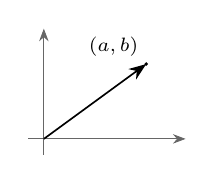
\begin{tikzpicture}[scale=.5]
  \draw[axis] (-.4,0)--(3.6,0); \draw[axis] (0,-.4)--(0,2.8);
  \draw[vec] (0,0)--(2.6,1.9);
  \fill (2.6,1.9) circle (1.4pt) node[above left=-1pt,font=\scriptsize] {$(a,b)$};
\end{tikzpicture}}{Elements of $\R^2$ can be thought of as points or as vectors.}%
A picture can aid our intuition. We will draw pictures in $\R^2$ because we can
sketch this space on two-dimensional surfaces such as paper and computer
screens. A typical element of $\R^2$ is a point $v=(a,b)$. Sometimes we think
of $v$ not as a point but as an arrow starting at the origin and ending at
$(a,b)$, as shown here. When we think of an element of $\R^2$ as an arrow, we
refer to it as a \emph{vector}.

\marginfig[1mm]{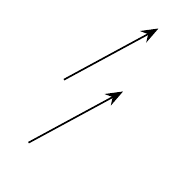
\begin{tikzpicture}[scale=.5]
  \draw[vec] (0,0)--(2.4,1.3); \draw[vec] (.9,1.6)--(3.3,2.9);
\end{tikzpicture}}{A vector.}%
When we think of vectors in $\R^2$ as arrows, we can move an arrow parallel to
itself (not changing its length or direction) and still think of it as the same
vector. With that viewpoint, you will often gain better understanding by
dispensing with the coordinate axes and the explicit coordinates and just
thinking of the vector, as shown in the figure here. The two arrows shown here
have the same length and same direction, so we think of them as the same
vector.

\marginnote{Mathematical models of the economy can have thousands of
variables, say $x_1,\dots,x_{5000}$, which means that we must work in
$\R^{5000}$. Such a space cannot be dealt with geometrically. However, the
algebraic approach works well. Thus our subject is called \emph{linear
algebra}.}%
Whenever we use pictures in $\R^2$ or use the somewhat vague language of points
and vectors, remember that these are just aids to our understanding, not
substitutes for the actual mathematics that we will develop. Although we cannot
draw good pictures in high-dimensional spaces, the elements of these spaces are
as rigorously defined as elements of $\R^2$.

For example, $(2,-3,17,\pi,\sqrt2)$ is an element of $\R^5$, and we may
casually refer to it as a point in $\R^5$ or a vector in $\R^5$ without
worrying about whether the geometry of $\R^5$ has any physical meaning.

Recall that we defined the sum of two elements of $\F^n$ to be the element of
$\F^n$ obtained by adding corresponding coordinates; see \ref{ax:1.13}. As we
will now see, addition has a simple geometric interpretation in the special
case of $\R^2$.

\marginfig{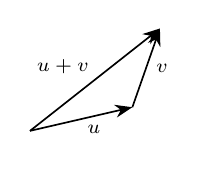
\begin{tikzpicture}[scale=.5]
  \draw[vec] (0,0)--node[below right=-2pt,font=\scriptsize]{$u$} (2.6,.6);
  \draw[vec] (2.6,.6)--node[right,font=\scriptsize]{$v$} (3.3,2.6);
  \draw[vec] (0,0)--node[above left=-2pt,font=\scriptsize]{$u+v$} (3.3,2.6);
\end{tikzpicture}}{The sum of two vectors.}%
Suppose we have two vectors $u$ and $v$ in $\R^2$ that we want to add. Move the
vector $v$ parallel to itself so that its initial point coincides with the end
point of the vector $u$, as shown here. The sum $u+v$ then equals the vector
whose initial point equals the initial point of $u$ and whose end point equals
the end point of the vector $v$, as shown here.

In the next definition, the $0$ on the right side of the displayed equation is
the list $0\in\F^n$.

\begin{definition}[Additive inverse in $\F^n$, $-x$]\label{ax:1.17}
For $x\in\F^n$, the \emph{additive inverse} of $x$, denoted by $-x$, is the
vector $-x\in\F^n$ such that
\[ x+(-x)=0. \]
Thus if $x=(x_1,\dots,x_n)$, then $-x=(-x_1,\dots,-x_n)$.
\end{definition}

\marginfig{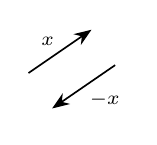
\begin{tikzpicture}[scale=.5]
  \draw[vec] (0.4,0.9)--node[above left=-2pt,font=\scriptsize]{$x$} (2.0,2.0);
  \draw[vec] (2.6,1.1)--node[below right=-2pt,font=\scriptsize]{$-x$} (1.0,0);
\end{tikzpicture}}{A vector and its additive inverse.}%
The additive inverse of a vector in $\R^2$ is the vector with the same length
but pointing in the opposite direction. The figure here illustrates this way of
thinking about the additive inverse in $\R^2$. As you can see, the vector
labeled $-x$ has the same length as the vector labeled $x$ but points in the
opposite direction.

Having dealt with addition in $\F^n$, we now turn to multiplication. We could
define a multiplication in $\F^n$ in a similar fashion, starting with two
elements of $\F^n$ and getting another element of $\F^n$ by multiplying
corresponding coordinates. Experience shows that this definition is not useful
for our purposes. Another type of multiplication, called scalar multiplication,
will be central to our subject. Specifically, we need to define what it means
to multiply an element of $\F^n$ by an element of $\F$.

\begin{definition}[Scalar multiplication in $\F^n$]\label{ax:1.18}
The \emph{product} of a number $\lambda$ and a vector in $\F^n$ is computed by
multiplying each coordinate of the vector by $\lambda$:
\[ \lambda(x_1,\dots,x_n) = (\lambda x_1,\dots,\lambda x_n); \]
here $\lambda\in\F$ and $(x_1,\dots,x_n)\in\F^n$.
\end{definition}

\marginnote{Scalar multiplication in $\F^n$ multiplies together a scalar and a
vector, getting a vector. In contrast, the dot product in $\R^2$ or $\R^3$
multiplies together two vectors and gets a scalar. Generalizations of the dot
product will become important in Chapter~6.}%
Scalar multiplication has a nice geometric interpretation in $\R^2$. If
$\lambda>0$ and $x\in\R^2$, then $\lambda x$ is the vector that points in the
same direction as $x$ and whose length is $\lambda$ times the length of $x$. In
other words, to get $\lambda x$, we shrink or stretch $x$ by a factor of
$\lambda$, depending on whether $\lambda<1$ or $\lambda>1$.

\marginfig[2mm]{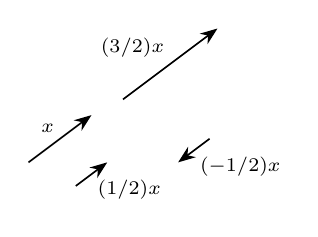
\begin{tikzpicture}[scale=.5]
  \draw[vec] (0,0)--node[above left=-2pt,font=\scriptsize]{$x$} (1.6,1.2);
  \draw[vec] (1.2,-.6)--node[below right=-2pt,font=\scriptsize]{$(1/2)x$} (2,0);
  \draw[vec] (2.4,1.6)--node[above left=-2pt,font=\scriptsize]{$(3/2)x$} (4.8,3.4);
  \draw[vec] (4.6,.6)--node[below right=-2pt,font=\scriptsize]{$(-1/2)x$} (3.8,0);
\end{tikzpicture}}{Scalar multiplication.}%
If $\lambda<0$ and $x\in\R^2$, then $\lambda x$ is the vector that points in
the direction opposite to that of $x$ and whose length is $\abs{\lambda}$ times
the length of $x$, as shown here.

\subsection{Digression on Fields}

A \emph{field} is a set containing at least two distinct elements called $0$
and $1$, along with operations of addition and multiplication satisfying all
properties listed in \ref{ax:1.3}. Thus $\R$ and $\C$ are fields, as is the set
of rational numbers along with the usual operations of addition and
multiplication. Another example of a field is the set $\{0,1\}$ with the usual
operations of addition and multiplication except that $1+1$ is defined to
equal $0$.

In this book we will not deal with fields other than $\R$ and $\C$. However,
many of the definitions, theorems, and proofs in linear algebra that work for
the fields $\R$ and $\C$ also work without change for arbitrary fields. If you
prefer to do so, throughout much of this book (except for Chapters~6 and~7,
which deal with inner product spaces) you can think of $\F$ as denoting an
arbitrary field instead of $\R$ or $\C$. For results (except in the inner
product chapters) that have as a hypothesis that $\F$ is $\C$, you can probably
replace that hypothesis with the hypothesis that $\F$ is an algebraically
closed field, which means that every nonconstant polynomial with coefficients
in $\F$ has a zero. A few results, such as Exercise~13 in Section~1C, require
the hypothesis on $\F$ that $1+1\ne0$.

% ------------------------------------------------------------------ exercises
\exercisesheading{1A}

\begin{exercise}
Show that $\alpha+\beta=\beta+\alpha$ for all $\alpha,\beta\in\C$.
\end{exercise}
\begin{solution}
Let $\alpha=a+bi$ and $\beta=c+di$ for some $a,b,c,d\in\R$. Then
\begin{align*}
\alpha+\beta &= (a+bi)+(c+di)\\
             &= (a+c)+(b+d)i\\
             &= (c+a)+(d+b)i\\
             &= (c+di)+(a+bi) = \beta+\alpha. \qedhere
\end{align*}
\end{solution}

\begin{exercise}
Show that $(\alpha+\beta)+\lambda=\alpha+(\beta+\lambda)$ for all
$\alpha,\beta,\lambda\in\C$.
\end{exercise}
\begin{solution}
Let $\alpha=a+bi$, $\beta=c+di$, and $\lambda=e+fi$ for some
$a,b,c,d,e,f\in\R$. Then
\begin{align*}
(\alpha+\beta)+\lambda &= \bigl((a+bi)+(c+di)\bigr)+(e+fi)\\
  &= \bigl((a+c)+(b+d)i\bigr)+(e+fi)\\
  &= (a+c+e)+(b+d+f)i\\
  &= \bigl(a+(c+e)\bigr)+\bigl(b+(d+f)\bigr)i\\
  &= (a+bi)+\bigl((c+di)+(e+fi)\bigr) = \alpha+(\beta+\lambda). \qedhere
\end{align*}
\end{solution}

\begin{exercise}
Show that $(\alpha\beta)\lambda=\alpha(\beta\lambda)$ for all
$\alpha,\beta,\lambda\in\C$.
\end{exercise}
\begin{solution}
Let $\alpha=a+bi$, $\beta=c+di$, and $\lambda=e+fi$ for some
$a,b,c,d,e,f\in\R$. Then
\begin{align*}
(\alpha\beta)\lambda &= \bigl((a+bi)(c+di)\bigr)(e+fi)\\
  &= \bigl((ac-bd)+(ad+bc)i\bigr)(e+fi)\\
  &= (ace-bde-adf-bcf)+(acf-bdf+ade+bce)i\\
  &= (ace-adf-bde-bcf)+(acf+ade+bce-bdf)i\\
  &= (a+bi)\bigl((ce-df)+(cf+de)i\bigr)\\
  &= (a+bi)\bigl((c+di)(e+fi)\bigr) = \alpha(\beta\lambda). \qedhere
\end{align*}
\end{solution}

\begin{exercise}
Show that $\lambda(\alpha+\beta)=\lambda\alpha+\lambda\beta$ for all
$\lambda,\alpha,\beta\in\C$.
\end{exercise}
\begin{solution}
Let $\alpha=a+bi$, $\beta=c+di$, and $\lambda=e+fi$ for some
$a,b,c,d,e,f\in\R$. Then
\begin{align*}
\lambda(\alpha+\beta) &= (e+fi)\bigl((a+bi)+(c+di)\bigr)\\
  &= (e+fi)\bigl((a+c)+(b+d)i\bigr)\\
  &= \bigl(e(a+c)-f(b+d)\bigr)+\bigl(e(b+d)+f(a+c)\bigr)i\\
  &= (ea-fb+ec-fd)+(eb+fa+ed+fc)i\\
  &= (ea-fb)+(eb+fa)i+(ec-fd)+(ed+fc)i\\
  &= (e+fi)(a+bi)+(e+fi)(c+di) = \lambda\alpha+\lambda\beta. \qedhere
\end{align*}
\end{solution}

\begin{exercise}
Show that for every $\alpha\in\C$, there exists a unique $\beta\in\C$ such that
$\alpha+\beta=0$.
\end{exercise}
\begin{solution}
Let $\alpha=a+bi$ for some $a,b\in\R$. We want to find $\beta=c+di$ such that
$\alpha+\beta=0$. This gives
\[ (a+bi)+(c+di) = (a+c)+(b+d)i = 0+0i. \]
Solving for $c$ and $d$, we get $c=-a$ and $d=-b$. Hence,
$\beta=c+di=-a-bi=-\alpha$.

To see that $\beta$ is unique, suppose there is another $\gamma\in\C$ such that
$\alpha+\gamma=0$. Then
\[ \beta=\beta+0=\beta+(\alpha+\gamma)=(\beta+\alpha)+\gamma=0+\gamma=\gamma. \]
Hence, $\beta$ is unique.
\end{solution}

\begin{exercise}
Show that for every $\alpha\in\C$ with $\alpha\ne0$, there exists a unique
$\beta\in\C$ such that $\alpha\beta=1$.
\end{exercise}
\begin{solution}
Let $\alpha=a+bi$ for some $a,b\in\R$ with $\alpha\ne0$. Then at least one of
$a$ or $b$ is nonzero. We want to find $\beta=c+di$ such that $\alpha\beta=1$.
If $a=0$, then $b\ne0$, and $\beta=1/(bi)=-i/b$. If $b=0$, then $a\ne0$, and
$\beta=1/a$. Otherwise, both $a$ and $b$ are nonzero. We then have
\[ (a+bi)(c+di) = (ac-bd)+(ad+bc)i = 1+0i. \]
Solving for $c$ and $d$, we get the system of equations
\[ \begin{cases} ac-bd=1\\ ad+bc=0 \end{cases}
   \implies
   \begin{cases} a^2c-abd=a\\ b^2c+abd=0. \end{cases} \]
Adding the two equations, we get
\[ (a^2+b^2)c=a \implies c=\frac{a}{a^2+b^2}. \]
Substituting this into the second equation, we get
\[ abd+b^2\frac{a}{a^2+b^2}=0 \implies d=\frac{-b}{a^2+b^2}. \]
Hence,
\[ \beta=c+di=\frac{a}{a^2+b^2}+\frac{-b}{a^2+b^2}\,i. \]
If $\gamma\in\C$ is another complex number such that $\alpha\gamma=1$, then
\[ \gamma=\gamma1=\gamma(\alpha\beta)=(\gamma\alpha)\beta=1\beta=\beta. \]
Hence, $\beta$ is unique.
\end{solution}

\begin{exercise}
Show that
\[ \frac{-1+\sqrt3\,i}{2} \]
is a cube root of $1$ (meaning that its cube equals $1$).
\end{exercise}
\begin{solution}
Note that the complex number given can be written as
\[ 1/2\bigl(-1+\sqrt3\,i\bigr). \]
Cubing $-1+\sqrt3\,i$, we get
\begin{align*}
\bigl(-1+\sqrt3\,i\bigr)^3
  &= (-1)^3+3(-1)^2\bigl(\sqrt3\,i\bigr)+3(-1)\bigl(\sqrt3\,i\bigr)^2+\bigl(\sqrt3\,i\bigr)^3\\
  &= -1+3\sqrt3\,i+3(-1)(-3)+\bigl(\sqrt3\,i\bigr)^3\\
  &= -1+3\sqrt3\,i+9-3\sqrt3\,i\\
  &= 8.
\end{align*}
Therefore,
\[ \biggl(\frac{-1+\sqrt3\,i}{2}\biggr)^{\!3}
   = \frac{\bigl(-1+\sqrt3\,i\bigr)^3}{8} = 8/8 = 1. \qedhere \]
\end{solution}

\begin{exercise}
Find two distinct square roots of $i$.
\end{exercise}
\begin{solution}
Let $z=a+bi$ for some $a,b\in\R$. We want to find $z$ such that $z^2=i$. This
gives
\[ (a+bi)^2 = a^2-b^2+2abi = 0+1i. \]
Solving for $a$ and $b$, we get the system of equations
\[ \begin{cases} a^2-b^2=0\\ 2ab=1. \end{cases} \]
The first equation yields $a=b$ or $a=-b$. If $a=b$, then the second equation
gives
\[ 2b^2=1 \implies b=\pm1/\sqrt2 \implies a=\pm1/\sqrt2. \]
If $a=-b$, this results in $-2b^2=1$, which has no solution when $b\in\R$.
Hence, the two distinct square roots of $i$ are
\[ 1/\sqrt2+1/\sqrt2\,i \quad\text{and}\quad
   -1/\sqrt2-1/\sqrt2\,i. \qedhere \]
\end{solution}

\begin{exercise}
Find $x\in\R^4$ such that
\[ (4,-3,1,7)+2x=(5,9,-6,8). \]
\end{exercise}
\begin{solution}
Let $x=(x_1,x_2,x_3,x_4)\in\R^4$. The equation becomes
\[ (4,-3,1,7)+2(x_1,x_2,x_3,x_4)=(5,9,-6,8), \]
which simplifies to the system of equations
\[ \begin{cases} 5=4+2x_1\\ 9=-3+2x_2\\ -6=1+2x_3\\ 8=7+2x_4 \end{cases}
   \implies
   \begin{cases} 2x_1=1\\ 2x_2=12\\ 2x_3=-7\\ 2x_4=1. \end{cases} \]
Therefore,
\[ x=\Bigl(1/2,\,6,\,-7/2,\,1/2\Bigr). \qedhere \]
\end{solution}

\begin{exercise}
Explain why there does not exist $\lambda\in\C$ such that
\[ \lambda(2-3i,\,5+4i,\,-6+7i)=(12-5i,\,7+22i,\,-32-9i). \]
\end{exercise}
\begin{solution}
Suppose there exists $\lambda\in\C$ such that
\[ \lambda(2-3i,\,5+4i,\,-6+7i)=(12-5i,\,7+22i,\,-32-9i). \]
This gives the system of equations
\[ \begin{cases} \lambda(2-3i)=12-5i\\ \lambda(5+4i)=7+22i\\ \lambda(-6+7i)=-32-9i. \end{cases} \]
Solving the first equation for $\lambda$, we get
\[ \lambda=\frac{12-5i}{2-3i}=\frac{(12-5i)(2+3i)}{(2-3i)(2+3i)}
   =\frac{24+36i-10i-15i^2}{4+9}=\frac{24+26i+15}{13}=3+2i. \]
However, using this value for $\lambda$ in the third equation, we get
\[ (3+2i)(-6+7i)=-18+21i-12i+14i^2=-18+9i-14=-32+9i\ne-32-9i. \]
Hence, no such $\lambda$ exists.
\end{solution}

\begin{exercise}
Show that $(x+y)+z=x+(y+z)$ for all $x,y,z\in\F^n$.
\end{exercise}
\begin{solution}
Let $x=(x_1,\dots,x_n)$, $y=(y_1,\dots,y_n)$, and $z=(z_1,\dots,z_n)$. Then
\begin{align*}
(x+y)+z &= \bigl((x_1,\dots,x_n)+(y_1,\dots,y_n)\bigr)+(z_1,\dots,z_n)\\
  &= (x_1+y_1,\dots,x_n+y_n)+(z_1,\dots,z_n)\\
  &= \bigl((x_1+y_1)+z_1,\dots,(x_n+y_n)+z_n\bigr)\\
  &= \bigl(x_1+(y_1+z_1),\dots,x_n+(y_n+z_n)\bigr)\\
  &= (x_1,\dots,x_n)+\bigl((y_1,\dots,y_n)+(z_1,\dots,z_n)\bigr)\\
  &= x+(y+z). \qedhere
\end{align*}
\end{solution}

\begin{exercise}
Show that $(ab)x=a(bx)$ for all $x\in\F^n$ and all $a,b\in\F$.
\end{exercise}
\begin{solution}
Let $x=(x_1,\dots,x_n)\in\F^n$ and $a,b\in\F$. Then
\begin{align*}
(ab)x &= (ab)(x_1,\dots,x_n)\\
      &= \bigl((ab)x_1,\dots,(ab)x_n\bigr)\\
      &= \bigl(a(bx_1),\dots,a(bx_n)\bigr)\\
      &= a(bx_1,\dots,bx_n)\\
      &= a(bx). \qedhere
\end{align*}
\end{solution}

\begin{exercise}
Show that $1x=x$ for all $x\in\F^n$.
\end{exercise}
\begin{solution}
Let $x=(x_1,\dots,x_n)\in\F^n$. Then
\begin{align*}
1x &= 1(x_1,\dots,x_n)\\
   &= (1x_1,\dots,1x_n)\\
   &= (x_1,\dots,x_n)\\
   &= x. \qedhere
\end{align*}
\end{solution}

\begin{exercise}
Show that $\lambda(x+y)=\lambda x+\lambda y$ for all $\lambda\in\F$ and all
$x,y\in\F^n$.
\end{exercise}
\begin{solution}
Let $x=(x_1,\dots,x_n)$ and $y=(y_1,\dots,y_n)$ be elements of $\F^n$ and
$\lambda\in\F$. Then
\begin{align*}
\lambda(x+y) &= \lambda\bigl((x_1,\dots,x_n)+(y_1,\dots,y_n)\bigr)\\
  &= \lambda(x_1+y_1,\dots,x_n+y_n)\\
  &= \bigl(\lambda(x_1+y_1),\dots,\lambda(x_n+y_n)\bigr)\\
  &= (\lambda x_1+\lambda y_1,\dots,\lambda x_n+\lambda y_n)\\
  &= (\lambda x_1,\dots,\lambda x_n)+(\lambda y_1,\dots,\lambda y_n)\\
  &= \lambda(x_1,\dots,x_n)+\lambda(y_1,\dots,y_n) = \lambda x+\lambda y. \qedhere
\end{align*}
\end{solution}

\begin{exercise}
Show that $(a+b)x=ax+bx$ for all $a,b\in\F$ and all $x\in\F^n$.
\end{exercise}
\begin{solution}
Let $x=(x_1,\dots,x_n)\in\F^n$ and $a,b\in\F$. Then
\begin{align*}
(a+b)x &= (a+b)(x_1,\dots,x_n)\\
       &= \bigl((a+b)x_1,\dots,(a+b)x_n\bigr)\\
       &= (ax_1+bx_1,\dots,ax_n+bx_n)\\
       &= (ax_1,\dots,ax_n)+(bx_1,\dots,bx_n)\\
       &= ax+bx. \qedhere
\end{align*}
\end{solution}

\axquote{``Can you do addition?'' the White Queen asked. ``What's one and one
and one and one and one and one and one and one and one and one?''\\
``I don't know,'' said Alice. ``I lost count.''}{\emph{Through the Looking
Glass}, Lewis Carroll}

% Source: book pp. 12--17 (PDF 26--31); solutions pp. 9--13.
\section{Definition of Vector Space}

The motivation for the definition of a vector space comes from properties of
addition and scalar multiplication in $\F^n$: Addition is commutative,
associative, and has an identity. Every element has an additive inverse. Scalar
multiplication is associative. Scalar multiplication by $1$ acts as expected.
Addition and scalar multiplication are connected by distributive properties.

We will define a vector space to be a set $V$ with an addition and a scalar
multiplication on $V$ that satisfy the properties in the paragraph above.

\begin{definition}[Addition, scalar multiplication]\label{ax:1.19}\leavevmode
\begin{itemize}
\item An \emph{addition} on a set $V$ is a function that assigns an element
  $u+v\in V$ to each pair of elements $u,v\in V$.
\item A \emph{scalar multiplication} on a set $V$ is a function that assigns an
  element $\lambda v\in V$ to each $\lambda\in\F$ and each $v\in V$.
\end{itemize}
\end{definition}

Now we are ready to give the formal definition of a vector space.

\begin{definition}[Vector space]\label{ax:1.20}
A \emph{vector space} is a set $V$ along with an addition on $V$ and a scalar
multiplication on $V$ such that the following properties hold.
\begin{axprops}
\item[commutativity] $u+v=v+u$ for all $u,v\in V$.
\item[associativity] $(u+v)+w=u+(v+w)$ and $(ab)v=a(bv)$ for all
  $u,v,w\in V$ and for all $a,b\in\F$.
\item[additive identity] There exists an element $0\in V$ such that $v+0=v$
  for all $v\in V$.
\item[additive inverse] For every $v\in V$, there exists $w\in V$ such that
  $v+w=0$.
\item[multiplicative identity] $1v=v$ for all $v\in V$.
\item[distributive properties] $a(u+v)=au+av$ and $(a+b)v=av+bv$ for all
  $a,b\in\F$ and all $u,v\in V$.
\end{axprops}
\end{definition}

The following geometric language sometimes aids our intuition.

\begin{definition}[Vector, point]\label{ax:1.21}
Elements of a vector space are called \emph{vectors} or \emph{points}.
\end{definition}

The scalar multiplication in a vector space depends on $\F$. Thus when we need
to be precise, we will say that $V$ is a \emph{vector space over} $\F$ instead
of saying simply that $V$ is a vector space. For example, $\R^n$ is a vector
space over $\R$, and $\C^n$ is a vector space over $\C$.

\begin{definition}[Real vector space, complex vector space]\label{ax:1.22}\leavevmode
\begin{itemize}
\item A vector space over $\R$ is called a \emph{real vector space}.
\item A vector space over $\C$ is called a \emph{complex vector space}.
\end{itemize}
\end{definition}

Usually the choice of $\F$ is either clear from the context or irrelevant. Thus
we often assume that $\F$ is lurking in the background without specifically
mentioning it.

\marginnote{The simplest vector space is $\{0\}$, which contains only one
point.}%
With the usual operations of addition and scalar multiplication, $\F^n$ is a
vector space over $\F$, as you should verify. The example of $\F^n$ motivated
our definition of vector space.

\begin{example}[$\F^\infty$]\label{ax:1.23}
$\F^\infty$ is defined to be the set of all sequences of elements of $\F$:
\[ \F^\infty = \{(x_1,x_2,\dots) : x_k\in\F \text{ for } k=1,2,\dots\}. \]
Addition and scalar multiplication on $\F^\infty$ are defined as expected:
\begin{align*}
(x_1,x_2,\dots)+(y_1,y_2,\dots) &= (x_1+y_1,x_2+y_2,\dots),\\
\lambda(x_1,x_2,\dots) &= (\lambda x_1,\lambda x_2,\dots).
\end{align*}
With these definitions, $\F^\infty$ becomes a vector space over $\F$, as you
should verify. The additive identity in this vector space is the sequence of
all $0$'s.
\end{example}

Our next example of a vector space involves a set of functions.

\begin{notation}[$\F^S$]\label{ax:1.24}\leavevmode
\begin{itemize}
\item If $S$ is a set, then $\F^S$ denotes the set of functions from $S$ to
  $\F$.
\item For $f,g\in\F^S$, the \emph{sum} $f+g\in\F^S$ is the function defined by
  \[ (f+g)(x) = f(x)+g(x) \]
  for all $x\in S$.
\item For $\lambda\in\F$ and $f\in\F^S$, the \emph{product} $\lambda f\in\F^S$
  is the function defined by
  \[ (\lambda f)(x) = \lambda f(x) \]
  for all $x\in S$.
\end{itemize}
\end{notation}

As an example of the notation above, if $S$ is the interval $[0,1]$ and
$\F=\R$, then $\R^{[0,1]}$ is the set of real-valued functions on the interval
$[0,1]$.

You should verify all three bullet points in the next example.

\begin{example}[$\F^S$ is a vector space]\label{ax:1.25}\leavevmode
\begin{itemize}
\item If $S$ is a nonempty set, then $\F^S$ (with the operations of addition
  and scalar multiplication as defined above) is a vector space over $\F$.
\item The additive identity of $\F^S$ is the function $0\colon S\to\F$ defined
  by
  \[ 0(x) = 0 \]
  for all $x\in S$.
\item For $f\in\F^S$, the additive inverse of $f$ is the function
  $-f\colon S\to\F$ defined by
  \[ (-f)(x) = -f(x) \]
  for all $x\in S$.
\end{itemize}
\end{example}

\marginnote{The elements of the vector space $\R^{[0,1]}$ are real-valued
functions on $[0,1]$, not lists. In general, a vector space is an abstract
entity whose elements might be lists, functions, or weird objects.}%
{\emergencystretch=2em
The vector space $\F^n$ is a special case of the vector space $\F^S$ because
each $(x_1,\dots,x_n)\in\F^n$ can be thought of as a function $x$ from the set
$\{1,2,\dots,n\}$ to $\F$ by writing $x(k)$ instead of $x_k$ for the
$k^{\text{th}}$ coordinate of $(x_1,\dots,x_n)$. In other words, we can think
of $\F^n$ as $\F^{\{1,2,\dots,n\}}$. Similarly, we can think of $\F^\infty$ as
$\F^{\{1,2,\dots\}}$.\par}

Soon we will see further examples of vector spaces, but first we need to
develop some of the elementary properties of vector spaces.

The definition of a vector space requires it to have an additive identity. The
next result states that this identity is unique.

\begin{result}[Unique additive identity]\label{ax:1.26}
A vector space has a unique additive identity.
\end{result}

\begin{proof}
Suppose $0$ and $0'$ are both additive identities for some vector space $V$.
Then
\[ 0' = 0'+0 = 0+0' = 0, \]
where the first equality holds because $0$ is an additive identity, the second
equality comes from commutativity, and the third equality holds because $0'$
is an additive identity. Thus $0'=0$, proving that $V$ has only one additive
identity.
\end{proof}

Each element $v$ in a vector space has an additive inverse, an element $w$ in
the vector space such that $v+w=0$. The next result shows that each element in
a vector space has only one additive inverse.

\begin{result}[Unique additive inverse]\label{ax:1.27}
Every element in a vector space has a unique additive inverse.
\end{result}

\begin{proof}
Suppose $V$ is a vector space. Let $v\in V$. Suppose $w$ and $w'$ are additive
inverses of $v$. Then
\[ w = w+0 = w+(v+w') = (w+v)+w' = 0+w' = w'. \]
Thus $w=w'$, as desired.
\end{proof}

Because additive inverses are unique, the following notation now makes sense.

\begin{notation}[$-v$, $w-v$]\label{ax:1.28}
Let $v,w\in V$. Then
\begin{itemize}
\item $-v$ denotes the additive inverse of $v$;
\item $w-v$ is defined to be $w+(-v)$.
\end{itemize}
\end{notation}

Almost all results in this book involve some vector space. To avoid having to
restate frequently that $V$ is a vector space, we now make the necessary
declaration once and for all.

\begin{notation}[$V$]\label{ax:1.29}
For the rest of this book, $V$ denotes a vector space over $\F$.
\end{notation}

In the next result, $0$ denotes a scalar (the number $0\in\F$) on the left side
of the equation and a vector (the additive identity of $V$) on the right side
of the equation.

\begin{result}[The number $0$ times a vector]\label{ax:1.30}
$0v=0$ for every $v\in V$.
\end{result}

\begin{proof}
For $v\in V$, we have
\[ 0v = (0+0)v = 0v+0v. \]
Adding the additive inverse of $0v$ to both sides of the equation above gives
$0=0v$, as desired.
\end{proof}

\marginnote[-14mm]{The result in \ref{ax:1.30} involves the additive identity of $V$
and scalar multiplication. The only part of the definition of a vector space
that connects vector addition and scalar multiplication is the distributive
property. Thus the distributive property must be used in the proof of
\ref{ax:1.30}.}%
In the next result, $0$ denotes the additive identity of $V$. Although their
proofs are similar, \ref{ax:1.30} and \ref{ax:1.31} are not identical. More
precisely, \ref{ax:1.30} states that the product of the scalar $0$ and any
vector equals the vector $0$, whereas \ref{ax:1.31} states that the product of
any scalar and the vector $0$ equals the vector $0$.

\begin{result}[A number times the vector $0$]\label{ax:1.31}
$a0=0$ for every $a\in\F$.
\end{result}

\begin{proof}
For $a\in\F$, we have
\[ a0 = a(0+0) = a0+a0. \]
Adding the additive inverse of $a0$ to both sides of the equation above gives
$0=a0$, as desired.
\end{proof}

Now we show that if an element of $V$ is multiplied by the scalar $-1$, then
the result is the additive inverse of the element of $V$.

\begin{result}[The number $-1$ times a vector]\label{ax:1.32}
$(-1)v=-v$ for every $v\in V$.
\end{result}

\begin{proof}
For $v\in V$, we have
\[ v+(-1)v = 1v+(-1)v = \bigl(1+(-1)\bigr)v = 0v = 0. \]
This equation says that $(-1)v$, when added to $v$, gives $0$. Thus $(-1)v$ is
the additive inverse of $v$, as desired.
\end{proof}

% ------------------------------------------------------------------ exercises
\exercisesheading{1B}

\begin{exercise}
Prove that $-(-v)=v$ for every $v\in V$.
\end{exercise}
\begin{solution}
Let $v\in V$. By the definition of additive inverse, we have
\[ v+(-v) = 0 = -(-v)+(-v). \]
Since additive inverses are unique, we conclude that $-(-v)=v$.
\end{solution}

\begin{exercise}
Suppose $a\in\F$, $v\in V$, and $av=0$. Prove that $a=0$ or $v=0$.
\end{exercise}
\begin{solution}
If $a=0$, then we are done. Suppose $a\ne0$. Then
\[ v = 1v = \frac1a(av) = \frac1a\cdot0 = 0. \qedhere \]
\end{solution}

\begin{exercise}
Suppose $v,w\in V$. Explain why there exists a unique $x\in V$ such that
$v+3x=w$.
\end{exercise}
\begin{solution}
\solnote{Manual Remark}{The solution says ``dividing by $3$'' in the sense that
we're dividing by the scalar $3$ in the field $\F$, not a vector in $V$.}
Solving for $x$ explicitly, we obtain
\[ 3x = w-v \implies x = (1/3)(w-v). \]
This shows that there exists $x\in V$ such that $v+3x=w$. To see that $x$ is
unique, suppose there exists another $y\in V$ such that $v+3y=w$. Then dividing
by $3$, we get
\[ 3x = w-v = 3y \implies x = y. \qedhere \]
\end{solution}

\begin{exercise}
The empty set is not a vector space. The empty set fails to satisfy only one of
the requirements listed in the definition of a vector space (\ref{ax:1.20}).
Which one?
\end{exercise}
\begin{solution}
The empty set fails to satisfy the requirement that there exists a zero vector
$0\in V$ such that $v+0=v$ for all $v\in V$ since it contains no elements.
\end{solution}

\begin{exercise}
Show that in the definition of a vector space (\ref{ax:1.20}), the additive
inverse condition can be replaced with the condition that
\[ 0v=0 \text{ for all } v\in V. \]
Here the $0$ on the left side is the number $0$, and the $0$ on the right side
is the additive identity of $V$.
\exnote{The phrase a ``condition can be replaced'' in a definition means that
the collection of objects satisfying the definition is unchanged if the
original condition is replaced with the new condition.}
\end{exercise}
\begin{solution}
Suppose that $0v=0$ for all $v\in V$. Let $v\in V$. Then
\[ v+(-1)v = 1v+(-1)v = \bigl(1+(-1)\bigr)v = 0v = 0. \]
Hence, $(-1)v$ is the additive inverse of $v$.

Conversely, suppose that for every $v\in V$, there exists an additive inverse
$-v\in V$ such that $v+(-v)=0$. Then $0v=(0+0)v=0v+0v$. Adding $-0v$ to both
sides, we get $0=0v$. Hence, $0v=0$ for all $v\in V$.
\end{solution}

\begin{exercise}
Let $\infty$ and $-\infty$ denote two distinct objects, neither of which is in
$\R$. Define an addition and scalar multiplication on $\R\cup\{\infty,-\infty\}$
as you could guess from the notation. Specifically, the sum and product of two
real numbers is as usual, and for $t\in\R$ define
\[ t\infty = \begin{cases} -\infty & \text{if } t<0,\\ 0 & \text{if } t=0,\\
     \infty & \text{if } t>0, \end{cases}
   \qquad
   t(-\infty) = \begin{cases} \infty & \text{if } t<0,\\ 0 & \text{if } t=0,\\
     -\infty & \text{if } t>0, \end{cases} \]
and
\begin{align*}
t+\infty = \infty+t = \infty+\infty &= \infty,\\
t+(-\infty) = (-\infty)+t = (-\infty)+(-\infty) &= -\infty,\\
\infty+(-\infty) = (-\infty)+\infty &= 0.
\end{align*}
With these operations of addition and scalar multiplication, is
$\R\cup\{\infty,-\infty\}$ a vector space over $\R$? Explain.
\end{exercise}
\begin{solution}
No, $\R\cup\{\infty,-\infty\}$ is not a vector space over $\R$ as it does not
satisfy the associative property of addition. Let $t\in\R\setminus\{0\}$. Then
\[ (t+\infty)+(-\infty) = \infty+(-\infty) = 0 \ne t = t+0
   = t+\bigl(\infty+(-\infty)\bigr). \qedhere \]
\end{solution}

\begin{exercise}
Suppose $S$ is a nonempty set. Let $V^S$ denote the set of functions from $S$
to $V$. Define a natural addition and scalar multiplication on $V^S$, and show
that $V^S$ is a vector space with these definitions.
\end{exercise}
\begin{solution}
Let $f,g\in V^S$ and $t\in\F$. Define addition and scalar multiplication as
follows:
\[ (f+g)(s) = f(s)+g(s), \quad (tf)(s) = t\bigl(f(s)\bigr) \]
for all $s\in S$. We will show that $V^S$ is a vector space with these
operations.
\begin{enumerate}[label=\arabic*)]
\item \textbf{Commutativity}: Let $f,g\in V^S$. Then for all $s\in S$,
  \[ (f+g)(s) = f(s)+g(s) = g(s)+f(s) = (g+f)(s). \]
\item \textbf{Associativity}: Let $f,g,h\in V^S$ and $t,u\in\F$. Then for all
  $s\in S$,
  \begin{align*}
  \bigl((f+g)+h\bigr)(s) &= (f+g)(s)+h(s)\\
    &= \bigl(f(s)+g(s)\bigr)+h(s)\\
    &= f(s)+\bigl(g(s)+h(s)\bigr)\\
    &= f(s)+(g+h)(s)\\
    &= \bigl(f+(g+h)\bigr)(s),
  \end{align*}
  and
  \begin{align*}
  \bigl((tu)f\bigr)(s) &= (tu)\bigl(f(s)\bigr)\\
    &= t\bigl(u(f(s))\bigr)\\
    &= t(uf)(s)\\
    &= \bigl(t(uf)\bigr)(s).
  \end{align*}
\item \textbf{Additive identity}: Let $0\in V$ be the additive identity in $V$.
  Define the zero function $0_S\in V^S$ by $0_S(s)=0$ for all $s\in S$. Then
  for all $f\in V^S$ and $s\in S$,
  \[ (f+0_S)(s) = f(s)+0_S(s) = f(s)+0 = f(s) = 0+f(s) = (0_S+f)(s). \]
  Hence, $0_S$ is the additive identity in $V^S$.
\item \textbf{Additive inverse}: Let $f\in V^S$. Define the function
  $-f\in V^S$ by $(-f)(s)=-f(s)$ for all $s\in S$. Then for all $s\in S$,
  \[ \bigl(f+(-f)\bigr)(s) = f(s)+(-f)(s) = f(s)+\bigl(-f(s)\bigr) = 0
     = 0_S(s). \]
  Hence, $-f$ is the additive inverse of $f$ in $V^S$.
\item \textbf{Multiplicative identity}: For all $f\in V^S$ and $s\in S$,
  \[ (1f)(s) = 1\bigl(f(s)\bigr) = f(s). \]
\item \textbf{Distributive properties}: Let $f,g\in V^S$ and $t,u\in\F$. Then
  for all $s\in S$,
  \begin{align*}
  \bigl((t+u)f\bigr)(s) &= (t+u)\bigl(f(s)\bigr)\\
    &= t\bigl(f(s)\bigr)+u\bigl(f(s)\bigr)\\
    &= (tf)(s)+(uf)(s)\\
    &= (tf+uf)(s),
  \end{align*}
  and
  \begin{align*}
  \bigl(t(f+g)\bigr)(s) &= t\bigl((f+g)(s)\bigr)\\
    &= t\bigl(f(s)+g(s)\bigr)\\
    &= t\bigl(f(s)\bigr)+t\bigl(g(s)\bigr)\\
    &= (tf)(s)+(tg)(s)\\
    &= (tf+tg)(s). \qedhere
  \end{align*}
\end{enumerate}
\end{solution}

\begin{exercise}
Suppose $V$ is a real vector space.
\begin{itemize}
\item The \emph{complexification} of $V$, denoted by $V_{\C}$, equals
  $V\times V$. An element of $V_{\C}$ is an ordered pair $(u,v)$, where
  $u,v\in V$, but we write this as $u+iv$.
\item Addition on $V_{\C}$ is defined by
  \[ (u_1+iv_1)+(u_2+iv_2) = (u_1+u_2)+i(v_1+v_2) \]
  for all $u_1,v_1,u_2,v_2\in V$.
\item Complex scalar multiplication on $V_{\C}$ is defined by
  \[ (a+bi)(u+iv) = (au-bv)+i(av+bu) \]
  for all $a,b\in\R$ and all $u,v\in V$.
\end{itemize}
Prove that with the definitions of addition and scalar multiplication as
above, $V_{\C}$ is a complex vector space.
\exnote{Think of $V$ as a subset of $V_{\C}$ by identifying $u\in V$ with
$u+i0$. The construction of $V_{\C}$ from $V$ can then be thought of as
generalizing the construction of $\C^n$ from $\R^n$.}
\end{exercise}
\begin{solution}
We prove that $V_{\C}$ is a complex vector space by verifying the vector space
axioms.
\begin{enumerate}[label=\arabic*)]
\item \textbf{Commutativity}: Let $u_1+v_1i,u_2+v_2i\in V_{\C}$. Then
  \begin{align*}
  (u_1+v_1i)+(u_2+v_2i) &= (u_1+u_2)+i(v_1+v_2)\\
    &= (u_2+u_1)+i(v_2+v_1) = (u_2+v_2i)+(u_1+v_1i).
  \end{align*}
\item \textbf{Associativity}: Let $u_1+v_1i,u_2+v_2i,u_3+v_3i\in V_{\C}$. Then
  \begin{align*}
  \bigl((u_1+v_1i)+(u_2+v_2i)\bigr)+(u_3+v_3i)
    &= \bigl((u_1+u_2)+i(v_1+v_2)\bigr)+(u_3+v_3i)\\
    &= \bigl((u_1+u_2)+u_3\bigr)+i\bigl((v_1+v_2)+v_3\bigr)\\
    &= \bigl(u_1+(u_2+u_3)\bigr)+i\bigl(v_1+(v_2+v_3)\bigr)\\
    &= (u_1+v_1i)+\bigl((u_2+v_2i)+(u_3+v_3i)\bigr).
  \end{align*}
  Similarly, let $a+bi,c+di\in\C$ and $u+vi\in V_{\C}$. Then
  \begin{align*}
  &\bigl((a+bi)(c+di)\bigr)(u+vi)\\
    &\qquad= \bigl((ac-bd)+i(ad+bc)\bigr)(u+vi)\\
    &\qquad= \bigl((ac-bd)u-(ad+bc)v\bigr)+i\bigl((ac-bd)v+(ad+bc)u\bigr)\\
    &\qquad= \bigl(a(cu-dv)-b(du+cv)\bigr)+i\bigl(a(du+cv)+b(cu-dv)\bigr)\\
    &\qquad= (a+bi)\bigl((cu-dv)+i(du+cv)\bigr)\\
    &\qquad= (a+bi)\bigl((c+di)(u+vi)\bigr).
  \end{align*}
\item \textbf{Additive identity}: Let $0\in V$ be the additive identity in $V$.
  Then for all $u+vi\in V_{\C}$,
  \[ (u+vi)+(0+0i) = (u+0)+i(v+0) = u+vi = (0+0i)+(u+vi). \]
  Hence, $0+0i$ is the additive identity in $V_{\C}$.
\item \textbf{Additive inverse}: Let $u+vi\in V_{\C}$. Then
  \[ (u+vi)+\bigl(-u+(-v)i\bigr) = (u-u)+i(v-v) = 0+0i. \]
  Hence, $-u+(-v)i$ is the additive inverse of $u+vi$ in $V_{\C}$.
\item \textbf{Multiplicative identity}: For all $u+vi\in V_{\C}$,
  \[ (1+0i)(u+vi) = (1u-0v)+i(1v+0u) = u+vi. \]
\item \textbf{Distributive properties}: Let $a+bi,c+di\in\C$ and
  $u_1+v_1i,u_2+v_2i\in V_{\C}$. Then
  \begin{align*}
  &(a+bi)\bigl((u_1+v_1i)+(u_2+v_2i)\bigr)\\
    &\qquad= (a+bi)\bigl((u_1+u_2)+i(v_1+v_2)\bigr)\\
    &\qquad= \bigl(a(u_1+u_2)-b(v_1+v_2)\bigr)+i\bigl(a(v_1+v_2)+b(u_1+u_2)\bigr)\\
    &\qquad= (au_1-bv_1)+i(av_1+bu_1)+(au_2-bv_2)+i(av_2+bu_2)\\
    &\qquad= (a+bi)(u_1+v_1i)+(a+bi)(u_2+v_2i),
  \end{align*}
  and
  \begin{align*}
  &\bigl((a+bi)+(c+di)\bigr)(u_1+v_1i)\\
    &\qquad= \bigl((a+c)+(b+d)i\bigr)(u_1+v_1i)\\
    &\qquad= \bigl((a+c)u_1-(b+d)v_1\bigr)+i\bigl((a+c)v_1+(b+d)u_1\bigr)\\
    &\qquad= (au_1-bv_1)+i(av_1+bu_1)+(cu_1-dv_1)+i(cv_1+du_1)\\
    &\qquad= (a+bi)(u_1+v_1i)+(c+di)(u_1+v_1i). \qedhere
  \end{align*}
\end{enumerate}
\end{solution}

% Source: book pp. 18--26 (PDF 32--40); solutions pp. 14--24, 168.
\section{Subspaces}

By considering subspaces, we can greatly expand our examples of vector spaces.

\begin{definition}[Subspace]\label{ax:1.33}
A subset $U$ of $V$ is called a \emph{subspace} of $V$ if $U$ is also a vector
space with the same additive identity, addition, and scalar multiplication as
on $V$.
\end{definition}

\marginnote{Some people use the terminology \emph{linear subspace}, which means
the same as subspace.}%
The next result gives the easiest way to check whether a subset of a vector
space is a subspace.

\begin{result}[Conditions for a subspace]\label{ax:1.34}
A subset $U$ of $V$ is a subspace of $V$ if and only if $U$ satisfies the
following three conditions.
\begin{axprops}
\item[additive identity] $0\in U$.
\item[closed under addition] $u,w\in U$ implies $u+w\in U$.
\item[closed under scalar multiplication] $a\in\F$ and $u\in U$ implies
  $au\in U$.
\end{axprops}
\end{result}

\begin{proof}
If $U$ is a subspace of $V$, then $U$ satisfies the three conditions above by
the definition of vector space.

Conversely, suppose $U$ satisfies the three conditions above. The first
condition ensures that the additive identity of $V$ is in $U$. The second
condition ensures that addition makes sense on $U$. The third condition ensures
that scalar multiplication makes sense on $U$.

\marginnote{The additive identity condition above could be replaced with the
condition that $U$ is nonempty (because then taking $u\in U$ and multiplying it
by $0$ would imply that $0\in U$). However, if a subset $U$ of $V$ is indeed a
subspace, then usually the quickest way to show that $U$ is nonempty is to show
that $0\in U$.}%
If $u\in U$, then $-u$ [which equals $(-1)u$ by \ref{ax:1.32}] is also in $U$
by the third condition above. Hence every element of $U$ has an additive
inverse in $U$.

The other parts of the definition of a vector space, such as associativity and
commutativity, are automatically satisfied for $U$ because they hold on the
larger space $V$. Thus $U$ is a vector space and hence is a subspace of $V$.
\end{proof}

The three conditions in the result above usually enable us to determine quickly
whether a given subset of $V$ is a subspace of $V$. You should verify all
assertions in the next example.

\begin{example}[Subspaces]\label{ax:1.35}\leavevmode
\begin{parts}
\item If $b\in\F$, then
  \[ \{(x_1,x_2,x_3,x_4)\in\F^4 : x_3=5x_4+b\} \]
  is a subspace of $\F^4$ if and only if $b=0$.
\item The set of continuous real-valued functions on the interval $[0,1]$ is a
  subspace of $\R^{[0,1]}$.
\item The set of differentiable real-valued functions on $\R$ is a subspace of
  $\R^{\R}$.
\item The set of differentiable real-valued functions $f$ on the interval
  $(0,3)$ such that $f'(2)=b$ is a subspace of $\R^{(0,3)}$ if and only if
  $b=0$.
\item The set of all sequences of complex numbers with limit $0$ is a subspace
  of $\C^\infty$.
\end{parts}
\end{example}

\marginnote{The set $\{0\}$ is the smallest subspace of $V$, and $V$ itself is
the largest subspace of $V$. The empty set is not a subspace of $V$ because a
subspace must be a vector space and hence must contain at least one element,
namely, an additive identity.}%
Verifying some of the items above shows the linear structure underlying parts
of calculus. For example, (b) above requires the result that the sum of two
continuous functions is continuous. As another example, (d) above requires the
result that for a constant $c$, the derivative of $cf$ equals $c$ times the
derivative of $f$.

The subspaces of $\R^2$ are precisely $\{0\}$, all lines in $\R^2$ containing
the origin, and $\R^2$. The subspaces of $\R^3$ are precisely $\{0\}$, all lines
in $\R^3$ containing the origin, all planes in $\R^3$ containing the origin, and
$\R^3$. To prove that all these objects are indeed subspaces is
straightforward---the hard part is to show that they are the only subspaces of
$\R^2$ and $\R^3$. That task will be easier after we introduce some additional
tools in the next chapter.

\subsection{Sums of Subspaces}

\marginnote{The union of subspaces is rarely a subspace (see Exercise~12),
which is why we usually work with sums rather than unions.}%
When dealing with vector spaces, we are usually interested only in subspaces,
as opposed to arbitrary subsets. The notion of the sum of subspaces will be
useful.

\begin{definition}[Sum of subspaces]\label{ax:1.36}
Suppose $V_1,\dots,V_m$ are subspaces of $V$. The \emph{sum} of
$V_1,\dots,V_m$, denoted by $V_1+\cdots+V_m$, is the set of all possible sums
of elements of $V_1,\dots,V_m$. More precisely,
\[ V_1+\cdots+V_m = \{v_1+\cdots+v_m : v_1\in V_1,\dots,v_m\in V_m\}. \]
\end{definition}

Let's look at some examples of sums of subspaces.

\begin{example}[A sum of subspaces of $\F^3$]\label{ax:1.37}
Suppose $U$ is the set of all elements of $\F^3$ whose second and third
coordinates equal $0$, and $W$ is the set of all elements of $\F^3$ whose first
and third coordinates equal $0$:
\[ U = \{(x,0,0)\in\F^3 : x\in\F\} \quad\text{and}\quad
   W = \{(0,y,0)\in\F^3 : y\in\F\}. \]
Then
\[ U+W = \{(x,y,0)\in\F^3 : x,y\in\F\}, \]
as you should verify.
\end{example}

\begin{example}[A sum of subspaces of $\F^4$]\label{ax:1.38}
Suppose
\[ U = \{(x,x,y,y)\in\F^4 : x,y\in\F\} \quad\text{and}\quad
   W = \{(x,x,x,y)\in\F^4 : x,y\in\F\}. \]
Using words rather than symbols, we could say that $U$ is the set of elements
of $\F^4$ whose first two coordinates equal each other and whose third and
fourth coordinates equal each other. Similarly, $W$ is the set of elements of
$\F^4$ whose first three coordinates equal each other.

To find a description of $U+W$, consider a typical element $(a,a,b,b)$ of $U$
and a typical element $(c,c,c,d)$ of $W$, where $a,b,c,d\in\F$. We have
\[ (a,a,b,b)+(c,c,c,d) = (a+c,a+c,b+c,b+d), \]
which shows that every element of $U+W$ has its first two coordinates equal to
each other. Thus\refstepcounter{theorem}
\[ U+W \subseteq \{(x,x,y,z)\in\F^4 : x,y,z\in\F\}.
   \tag*{\thetheorem}\label{ax:1.39} \]

To prove the inclusion in the other direction, suppose $x,y,z\in\F$. Then
\[ (x,x,y,z) = (x,x,y,y)+(0,0,0,z-y), \]
where the first vector on the right is in $U$ and the second vector on the
right is in $W$. Thus $(x,x,y,z)\in U+W$, showing that the inclusion
\ref{ax:1.39} also holds in the opposite direction. Hence
\[ U+W = \{(x,x,y,z)\in\F^4 : x,y,z\in\F\}, \]
which shows that $U+W$ is the set of elements of $\F^4$ whose first two
coordinates equal each other.
\end{example}

The next result states that the sum of subspaces is a subspace, and is in fact
the smallest subspace containing all the summands (which means that every
subspace containing all the summands also contains the sum).

\begin{result}[Sum of subspaces is the smallest containing subspace]\label{ax:1.40}
Suppose $V_1,\dots,V_m$ are subspaces of $V$. Then $V_1+\cdots+V_m$ is the
smallest subspace of $V$ containing $V_1,\dots,V_m$.
\end{result}

\begin{proof}
The reader can verify that $V_1+\cdots+V_m$ contains the additive identity $0$
and is closed under addition and scalar multiplication. Thus \ref{ax:1.34}
implies that $V_1+\cdots+V_m$ is a subspace of $V$.

\marginnote{Sums of subspaces in the theory of vector spaces are analogous to
unions of subsets in set theory. Given two subspaces of a vector space, the
smallest subspace containing them is their sum. Analogously, given two subsets
of a set, the smallest subset containing them is their union.}%
The subspaces $V_1,\dots,V_m$ are all contained in $V_1+\cdots+V_m$ (to see
this, consider sums $v_1+\cdots+v_m$ where all except one of the $v_k$'s are
$0$). Conversely, every subspace of $V$ containing $V_1,\dots,V_m$ contains
$V_1+\cdots+V_m$ (because subspaces must contain all finite sums of their
elements). Thus $V_1+\cdots+V_m$ is the smallest subspace of $V$ containing
$V_1,\dots,V_m$.
\end{proof}

\subsection{Direct Sums}

Suppose $V_1,\dots,V_m$ are subspaces of $V$. Every element of
$V_1+\cdots+V_m$ can be written in the form
\[ v_1+\cdots+v_m, \]
where each $v_k\in V_k$. Of special interest are cases in which each vector in
$V_1+\cdots+V_m$ can be represented in the form above in only one way. This
situation is so important that it gets a special name (direct sum) and a
special symbol ($\oplus$).

\begin{definition}[Direct sum, $\oplus$]\label{ax:1.41}
Suppose $V_1,\dots,V_m$ are subspaces of $V$.
\begin{itemize}
\item The sum $V_1+\cdots+V_m$ is called a \emph{direct sum} if each element of
  $V_1+\cdots+V_m$ can be written in only one way as a sum $v_1+\cdots+v_m$,
  where each $v_k\in V_k$.
\item If $V_1+\cdots+V_m$ is a direct sum, then $V_1\oplus\cdots\oplus V_m$
  denotes $V_1+\cdots+V_m$, with the $\oplus$ notation serving as an indication
  that this is a direct sum.
\end{itemize}
\end{definition}

\begin{example}[A direct sum of two subspaces]\label{ax:1.42}
Suppose $U$ is the subspace of $\F^3$ of those vectors whose last coordinate
equals $0$, and $W$ is the subspace of $\F^3$ of those vectors whose first two
coordinates equal $0$:
\[ U = \{(x,y,0)\in\F^3 : x,y\in\F\} \quad\text{and}\quad
   W = \{(0,0,z)\in\F^3 : z\in\F\}. \]
Then $\F^3=U\oplus W$, as you should verify.
\end{example}

\marginnote[6mm]{To produce $\oplus$ in \TeX, type \texttt{\string\oplus}.}%
\begin{example}[A direct sum of multiple subspaces]\label{ax:1.43}
Suppose $V_k$ is the subspace of $\F^n$ of those vectors whose coordinates are
all $0$, except possibly in the $k^{\text{th}}$ slot; for example,
$V_2=\{(0,x,0,\dots,0)\in\F^n : x\in\F\}$. Then
\[ \F^n = V_1\oplus\cdots\oplus V_n, \]
as you should verify.
\end{example}

Sometimes nonexamples add to our understanding as much as examples.

\begin{example}[A sum that is not a direct sum]\label{ax:1.44}
Suppose
\begin{align*}
V_1 &= \{(x,y,0)\in\F^3 : x,y\in\F\},\\
V_2 &= \{(0,0,z)\in\F^3 : z\in\F\},\\
V_3 &= \{(0,y,y)\in\F^3 : y\in\F\}.
\end{align*}
Then $\F^3=V_1+V_2+V_3$ because every vector $(x,y,z)\in\F^3$ can be written as
\[ (x,y,z) = (x,y,0)+(0,0,z)+(0,0,0), \]
where the first vector on the right side is in $V_1$, the second vector is in
$V_2$, and the third vector is in $V_3$.

However, $\F^3$ does not equal the direct sum of $V_1,V_2,V_3$, because the
vector $(0,0,0)$ can be written in more than one way as a sum $v_1+v_2+v_3$,
with each $v_k\in V_k$. Specifically, we have
\[ (0,0,0) = (0,1,0)+(0,0,1)+(0,-1,-1) \]
and, of course,
\[ (0,0,0) = (0,0,0)+(0,0,0)+(0,0,0), \]
where the first vector on the right side of each equation above is in $V_1$,
the second vector is in $V_2$, and the third vector is in $V_3$. Thus the sum
$V_1+V_2+V_3$ is not a direct sum.
\end{example}

\marginnote[-8mm]{The symbol $\oplus$, which is a plus sign inside a circle, reminds
us that we are dealing with a special type of sum of subspaces---each element
in the direct sum can be represented in only one way as a sum of elements from
the specified subspaces.}%
The definition of direct sum requires every vector in the sum to have a unique
representation as an appropriate sum. The next result shows that when deciding
whether a sum of subspaces is a direct sum, we only need to consider whether
$0$ can be uniquely written as an appropriate sum.

\begin{result}[Condition for a direct sum]\label{ax:1.45}
Suppose $V_1,\dots,V_m$ are subspaces of $V$. Then $V_1+\cdots+V_m$ is a direct
sum if and only if the only way to write $0$ as a sum $v_1+\cdots+v_m$, where
each $v_k\in V_k$, is by taking each $v_k$ equal to $0$.
\end{result}

\begin{proof}
First suppose $V_1+\cdots+V_m$ is a direct sum. Then the definition of direct
sum implies that the only way to write $0$ as a sum $v_1+\cdots+v_m$, where each
$v_k\in V_k$, is by taking each $v_k$ equal to $0$.

Now suppose that the only way to write $0$ as a sum $v_1+\cdots+v_m$, where
each $v_k\in V_k$, is by taking each $v_k$ equal to $0$. To show that
$V_1+\cdots+V_m$ is a direct sum, let $v\in V_1+\cdots+V_m$. We can write
\[ v = v_1+\cdots+v_m \]
for some $v_1\in V_1,\dots,v_m\in V_m$. To show that this representation is
unique, suppose we also have
\[ v = u_1+\cdots+u_m, \]
where $u_1\in V_1,\dots,u_m\in V_m$. Subtracting these two equations, we have
\[ 0 = (v_1-u_1)+\cdots+(v_m-u_m). \]
Because $v_1-u_1\in V_1,\dots,v_m-u_m\in V_m$, the equation above implies that
each $v_k-u_k$ equals $0$. Thus $v_1=u_1,\dots,v_m=u_m$, as desired.
\end{proof}

\marginnote{The symbol $\iff$ used below means ``if and only if''; this symbol
could also be read to mean ``is equivalent to''.}%
The next result gives a simple condition for testing whether a sum of two
subspaces is a direct sum.

\begin{result}[Direct sum of two subspaces]\label{ax:1.46}
Suppose $U$ and $W$ are subspaces of $V$. Then
\[ U+W \text{ is a direct sum} \iff U\cap W=\{0\}. \]
\end{result}

\begin{proof}
First suppose that $U+W$ is a direct sum. If $v\in U\cap W$, then
$0=v+(-v)$, where $v\in U$ and $-v\in W$. By the unique representation of $0$
as the sum of a vector in $U$ and a vector in $W$, we have $v=0$. Thus
$U\cap W=\{0\}$, completing the proof in one direction.

To prove the other direction, now suppose $U\cap W=\{0\}$. To prove that $U+W$
is a direct sum, suppose $u\in U$, $w\in W$, and
\[ 0 = u+w. \]
To complete the proof, we only need to show that $u=w=0$ (by \ref{ax:1.45}).
The equation above implies that $u=-w\in W$. Thus $u\in U\cap W$. Hence $u=0$,
which by the equation above implies that $w=0$, completing the proof.
\end{proof}

\marginnote{Sums of subspaces are analogous to unions of subsets. Similarly,
direct sums of subspaces are analogous to disjoint unions of subsets. No two
subspaces of a vector space can be disjoint, because both contain $0$. So
disjointness is replaced, at least in the case of two subspaces, with the
requirement that the intersection equal $\{0\}$.}%
The result above deals only with the case of two subspaces. When asking about
a possible direct sum with more than two subspaces, it is not enough to test
that each pair of the subspaces intersect only at $0$. To see this, consider
Example~\ref{ax:1.44}. In that nonexample of a direct sum, we have
$V_1\cap V_2=V_1\cap V_3=V_2\cap V_3=\{0\}$.

% ------------------------------------------------------------------ exercises
\exercisesheading{1C}

\begin{exercise}
For each of the following subsets of $\F^3$, determine whether it is a subspace
of $\F^3$.
\begin{parts}
\item $\{(x_1,x_2,x_3)\in\F^3 : x_1+2x_2+3x_3=0\}$
\item $\{(x_1,x_2,x_3)\in\F^3 : x_1+2x_2+3x_3=4\}$
\item $\{(x_1,x_2,x_3)\in\F^3 : x_1x_2x_3=0\}$
\item $\{(x_1,x_2,x_3)\in\F^3 : x_1=5x_3\}$
\end{parts}
\end{exercise}
\begin{solution}
Let $U$ be the subset of $\F^3$ in question.
\begin{parts}
\item Since the zero vector $(0,0,0)$ satisfies $0+2(0)+3(0)=0$, $U$ is
  nonempty. Let $u=(u_1,u_2,u_3)$ and $v=(v_1,v_2,v_3)$ be elements of $U$.
  Then
  \[ (u_1+v_1)+2(u_2+v_2)+3(u_3+v_3)
     = (u_1+2u_2+3u_3)+(v_1+2v_2+3v_3) = 0+0 = 0. \]
  Hence, $u+v$ is in $U$. Let $a\in\F$. Then
  \[ au_1+2(au_2)+3(au_3) = a(u_1+2u_2+3u_3) = a\cdot0 = 0. \]
  Hence, $au$ is in $U$. Therefore, $U$ is a subspace of $\F^3$.
\item The zero vector $(0,0,0)$ does not satisfy $0+2(0)+3(0)=4$, so $U$ does
  not contain the zero vector. Hence, it is not a subspace of $\F^3$.
\item Suppose $u=(1,0,0)$ and $v=(0,1,1)$. Then $u$ and $v$ are in $U$ since
  $1\cdot0\cdot0=0$ and $0\cdot1\cdot1=0$. However, $u+v=(1,1,1)$ is not in $U$
  since $1\cdot1\cdot1=1\ne0$. Hence, $U$ is not closed under addition and is
  not a subspace of $\F^3$.
\item Since the zero vector $(0,0,0)$ satisfies $0=5(0)$, $U$ is nonempty. Let
  $u=(u_1,u_2,u_3)$ and $v=(v_1,v_2,v_3)$ be elements of $U$. Then
  \[ u_1+v_1 = 5u_3+5v_3 = 5(u_3+v_3). \]
  Hence, $u+v$ is in $U$. Let $a\in\F$. Then
  \[ au_1 = a(5u_3) = 5(au_3). \]
  Hence, $au$ is in $U$. Therefore, $U$ is a subspace of $\F^3$.
\end{parts}
\end{solution}

\begin{exercise}
Verify all assertions about subspaces in Example~\ref{ax:1.35}.
\end{exercise}
\begin{solution}
Let $U$ be the subset of $\F^4$ in question.
\begin{parts}
\item Suppose $U$ is a subspace of $\F^4$. Then it must contain the zero vector
  $(0,0,0,0)$. Then $0=5(0)+b$, which implies $b=0$.

  Conversely, suppose $b=0$. Then
  $U=\{(x_1,x_2,x_3,x_4)\in\F^4 \mid x_3=5x_4\}$. The proof is similar to that
  of Exercise~1C1~(d), hence $U$ is a subspace of $\F^4$.
\item Note that the $0$ function on $[0,1]$ is continuous, so $0\in U$. Let
  $f,g\in U$ be continuous functions. Then $f+g$ is continuous, so $f+g\in U$.
  Let $a\in\R$. Then $af$ is continuous, so $af\in U$. Therefore, $U$ is a
  subspace of $\R^{[0,1]}$.
\item Since the derivative of the $0$ function is the $0$ function, $0\in U$.
  Let $f,g\in U$ be differentiable functions. Then $f+g$ is differentiable, so
  $f+g\in U$. Let $a\in\R$. Then $af$ is differentiable, so $af\in U$.
  Therefore, $U$ is a subspace of $\R^{\R}$.
\item Suppose $U$ is a subspace of $\R^{(0,3)}$. Then it must contain the $0$
  function on $(0,3)$. Then $0'=0=b$, which implies $b=0$.

  Conversely, suppose $b=0$. Then $U=\{f\in\R^{(0,3)} \mid f'(2)=0\}$. Let
  $f,g\in U$ be differentiable functions such that $f'(2)=g'(2)=0$. Then
  \[ (f+g)'(2) = f'(2)+g'(2) = 0+0 = 0, \]
  so $f+g\in U$. Let $a\in\R$. Then
  \[ (af)'(2) = af'(2) = a\cdot0 = 0, \]
  so $af\in U$. Therefore, $U$ is a subspace of $\R^{(0,3)}$.
\item Let $U$ be the set of all sequences of complex numbers with limit $0$.
  Then the zero sequence is in $U$. Let $(z_n),(w_n)\in U$ be sequences with
  limit $0$. Then
  \[ \lim_{n\to\infty}(z_n+w_n) = \lim_{n\to\infty}z_n+\lim_{n\to\infty}w_n
     = 0+0 = 0, \]
  so $(z_n)+(w_n)\in U$. Let $a\in\C$. Then
  \[ \lim_{n\to\infty}(az_n) = a\lim_{n\to\infty}z_n = a\cdot0 = 0, \]
  so $a(z_n)\in U$. Therefore, $U$ is a subspace of $\C^\infty$.
\end{parts}
\end{solution}

\begin{exercise}
Show that the set of differentiable real-valued functions $f$ on the interval
$(-4,4)$ such that $f'(-1)=3f(2)$ is a subspace of $\R^{(-4,4)}$.
\end{exercise}
\begin{solution}
Let $U$ be the set in question. Then the zero function is in $U$ since
$0'(-1)=0=3\cdot0=3\cdot0(2)$. Let $f,g\in U$ be differentiable functions such
that $f'(-1)=3f(2)$ and $g'(-1)=3g(2)$. Then
\[ (f+g)'(-1) = f'(-1)+g'(-1) = 3f(2)+3g(2) = 3\bigl(f(2)+g(2)\bigr)
   = 3(f+g)(2), \]
so $f+g\in U$. Let $a\in\R$. Then
\[ (af)'(-1) = af'(-1) = a\cdot3f(2) = 3(af)(2), \]
so $af\in U$. Therefore, $U$ is a subspace of $\R^{(-4,4)}$.
\end{solution}

\begin{exercise}
Suppose $b\in\R$. Show that the set of continuous real-valued functions $f$ on
the interval $[0,1]$ such that $\int_0^1 f=b$ is a subspace of $\R^{[0,1]}$ if
and only if $b=0$.
\end{exercise}
\begin{solution}
Let $U$ be the set in question. Suppose $U$ is a subspace of $\R^{[0,1]}$. Then
it must contain the zero function on $[0,1]$. Then
\[ \int_0^1 0 = 0 = b, \]
which implies $b=0$.

Conversely, suppose $b=0$. Then
\[ U = \biggl\{f\in\R^{[0,1]} \biggm| \int_0^1 f=0\biggr\}. \]
The zero function is in $U$ since $\int_0^1 0=0$. Let $f,g\in U$ be continuous
functions such that $\int_0^1 f=\int_0^1 g=0$. Then
\[ \int_0^1 (f+g) = \int_0^1 f+\int_0^1 g = 0+0 = 0, \]
so $f+g\in U$. Let $a\in\R$. Then
\[ \int_0^1 (af) = a\int_0^1 f = a\cdot0 = 0, \]
so $af\in U$. Therefore, $U$ is a subspace of $\R^{[0,1]}$.
\end{solution}

\begin{exercise}
Is $\R^2$ a subspace of the complex vector space $\C^2$?
\end{exercise}
\begin{solution}
No, $\R^2$ is not a subspace of $\C^2$. Let $u=(1,0)\in\R^2$ and $a=i\in\C$.
Then $au=(i,0)\notin\R^2$, so $\R^2$ is not closed under scalar multiplication
and is not a subspace of $\C^2$.
\end{solution}

\begin{exercise}\leavevmode
\begin{parts}
\item Is $\{(a,b,c)\in\R^3 : a^3=b^3\}$ a subspace of $\R^3$?
\item Is $\{(a,b,c)\in\C^3 : a^3=b^3\}$ a subspace of $\C^3$?
\end{parts}
\end{exercise}
\begin{solution}
\solnote{Manual Remark}{Here, I present an elementary argument that does not
require the use of De Moivre's Theorem; rather, I arrive at the conclusion
directly. However, readers who are familiar with it may find it easier to note
that the complex number $1$ has three cube roots of unity. Other readers may
also use Vieta's formulas to arrive at the same polynomial in $\omega$ to obtain
$1+\omega=-\omega^2$.}
Let $U$ be the subset in question.
\begin{parts}
\item Since the zero vector $(0,0,0)$ satisfies $0^3=0^3$, $U$ is nonempty. Let
  $x=(x_1,x_2,x_3)$ and $y=(y_1,y_2,y_3)$ be elements of $U$. Then
  $x_1^3=x_2^3$ and $y_1^3=y_2^3$ both imply that $x_1=x_2$ and $y_1=y_2$.
  Hence,
  \[ (x_1+y_1)^3 = (x_2+y_2)^3, \]
  so $x+y\in U$. Let $a\in\R$. Then
  \[ (ax_1)^3 = a^3x_1^3 = a^3x_2^3 = (ax_2)^3, \]
  so $ax\in U$. Therefore, $U$ is a subspace of $\R^3$.
\item No, $U$ is not a subspace of $\C^3$. To see this, consider the cubic
  polynomial $x^3-1=0$. This polynomial has three distinct roots in $\C$ as
  follows:
  \[ x^3-1 = (x-1)(x^2+x+1) = 0 \]
  Applying the quadratic formula to $x^2+x+1=0$, we get
  \[ x = \frac{-1\pm\sqrt{(-1)^2-4(1)(1)}}{2(1)} = \frac{-1\pm i\sqrt3}{2}. \]
  Let
  \[ \omega = \frac{-1+i\sqrt3}{2}. \]
  Then $\omega^3=1$, and
  \[ \omega^2 = \frac{-1-i\sqrt3}{2}. \]
  Moreover, it is not hard to see that $\omega+\omega^2=-1$. Let $u=(1,1,0)$
  and $v=(\omega,1,0)$. Then $u,v\in U$ since $1^3=1^3$ and $\omega^3=1^3$.
  Then $u+v=(1+\omega,2,0)$. However,
  \[ (1+\omega)^3 = 1+3\omega+3\omega^2+\omega^3 = 1+3(-1)+1 = -1 \ne 2^3 = 8. \]
  Hence, $u+v\notin U$, so $U$ is not closed under addition and is not a
  subspace of $\C^3$.
\end{parts}
\end{solution}

\begin{exercise}
Prove or give a counterexample: If $U$ is a nonempty subset of $\R^2$ such that
$U$ is closed under addition and under taking additive inverses (meaning
$-u\in U$ whenever $u\in U$), then $U$ is a subspace of $\R^2$.
\end{exercise}
\begin{solution}
Consider the subset $\Q^2$ of $\R^2$. Then $\Q^2$ is nonempty because
$(0,0)\in\Q^2$, closed under addition since the sum of any two rational numbers
is rational, and closed under taking additive inverses since the additive
inverse of a rational number is rational. However, for any irrational number
$r\in\R$, the vector $(r,0)=r(1,0)\in\R^2$ is not in $\Q^2$. Hence, $\Q^2$ is
not closed under scalar multiplication and is not a subspace of $\R^2$.
Therefore, the statement is false.
\end{solution}

\begin{exercise}
Give an example of a nonempty subset $U$ of $\R^2$ such that $U$ is closed
under scalar multiplication, but $U$ is not a subspace of $\R^2$.
\end{exercise}
\begin{solution}
Consider the subset
\[ U = \{(x,0) \mid x\in\R\}\cup\{(0,y) \mid y\in\R\}. \]
Then $U$ is nonempty since $(1,0)\in U$, and it is closed under scalar
multiplication since any scalar multiple of $(1,0)$ or $(0,1)$ is still in
$U$. However, $U$ is not closed under addition since
$(1,0)+(0,1)=(1,1)\notin U$. Hence, $U$ is not a subspace of $\R^2$.
\end{solution}

\begin{exercise}
A function $f\colon\R\to\R$ is called \emph{periodic} if there exists a
positive number $p$ such that $f(x)=f(x+p)$ for all $x\in\R$. Is the set of
periodic functions from $\R$ to $\R$ a subspace of $\R^{\R}$? Explain.
\end{exercise}
\begin{solution}
It is not a subspace of $\R^{\R}$. Consider the periodic functions
$f(x)=\cos x$ and $g(x)=\cos\sqrt2\,x$. Then the sum $f+g$ attains a maximum
value of $2$ at $0$. If $f+g$ were periodic with period $p$, then
$(f+g)(p)=(f+g)(0)=2$. This implies $\cos p=\cos p\sqrt2=1$. Then $p=2\pi m$
and $p\sqrt2=2\pi n$ for positive integers $m$ and $n$. Since $p\sqrt2=2\pi n$
implies $p=\sqrt2\pi n$, we have
\[ 2\pi m = \sqrt2\pi n \implies \sqrt2 = \frac nm, \]
which is a contradiction, since $\sqrt2$ is irrational. Then $f+g$ is not
periodic.
\end{solution}

\begin{exercise}
Suppose $V_1$ and $V_2$ are subspaces of $V$. Prove that the intersection
$V_1\cap V_2$ is a subspace of $V$.
\end{exercise}
\begin{solution}
Let $U=V_1\cap V_2$. Since both $V_1$ and $V_2$ are subspaces of $V$, they both
contain the zero vector of $V$. Hence, $0\in U$, so $U$ is nonempty. Let
$u,v\in U$. Then $u,v\in V_1$ and $u,v\in V_2$. Since both $V_1$ and $V_2$ are
subspaces, they are closed under addition. Therefore, $u+v\in V_1$ and
$u+v\in V_2$, which implies that $u+v\in U$. Let $a\in\F$. Then since both
$V_1$ and $V_2$ are closed under scalar multiplication, we have that
$au\in V_1$ and $au\in V_2$, which implies that $au\in U$. Therefore, $U$ is a
subspace of $V$.
\end{solution}

\begin{exercise}
Prove that the intersection of every collection of subspaces of $V$ is a
subspace of $V$.
\end{exercise}
\begin{solution}
Let $\mathcal{C}$ be a collection of subspaces of $V$, and let
\[ U = \bigcap_{W\in\mathcal{C}} W. \]
Since each subspace in $\mathcal{C}$ contains the zero vector, $0\in U$, so $U$
is nonempty. Let $u,v\in U$. Then $u,v\in W$ for all $W\in\mathcal{C}$. Since
each $W$ is a subspace, they are closed under addition, so $u+v\in W$ for all
$W\in\mathcal{C}$, which implies $u+v\in U$. Let $a\in\F$. Then $au\in W$ for
all $W\in\mathcal{C}$, which implies $au\in U$. Therefore, $U$ is a subspace of
$V$.
\end{solution}

\begin{exercise}
Prove that the union of two subspaces of $V$ is a subspace of $V$ if and only
if one of the subspaces is contained in the other.
\end{exercise}
\begin{solution}
Let $U,W$ be subspaces of $V$. Suppose $U\subseteq W$. Then $U\cup W=W$, which
is a subspace of $V$. Similarly, if $W\subseteq U$, then $U\cup W=U$, which is
a subspace of $V$.

Conversely, suppose $U\cup W$ is a subspace of $V$. If neither $U\subseteq W$
nor $W\subseteq U$, then there exist $u\in U\setminus W$ and
$w\in W\setminus U$. Since $U\cup W$ is a subspace, it must be closed under
addition. Then $u+w\in U\cup W$. However, $u+w\notin U$ because if it were,
then $w=(u+w)-u\in U$, which is a contradiction. Similarly, $u+w\notin W$
because if it were, then $u=(u+w)-w\in W$, which is also a contradiction.
Hence, $u+w\notin U\cup W$, which contradicts the assumption that $U\cup W$ is
a subspace. Therefore, one of the subspaces must be contained in the other.
\end{solution}

\begin{exercise}
Prove that the union of three subspaces of $V$ is a subspace of $V$ if and only
if one of the subspaces contains the other two.
\exnote{This exercise is surprisingly harder than Exercise~12, possibly because
this exercise is not true if we replace $\F$ with a field containing only two
elements.}
\end{exercise}
\begin{solution}
\solnote{Axler Note}{This result fails when the field has only two elements.}
\solnote{Manual Remark}{The proof of this exercise is more involved than the
proof of Exercise~1C12 in that it requires a more careful analysis of the
possible relationships between the three subspaces.}
\solnote{Appendix}{See the alternate proof at the end of this solution for a
more elegant proof of this result, which implicitly uses the result that
$\operatorname{char}(\F)\ne2$.}
Let $U_1,U_2,U_3$ be subspaces of $V$. Without loss of generality, suppose
$U_2\subseteq U_1$ and $U_3\subseteq U_1$. Then $U_1\cup U_2\cup U_3=U_1$,
which is a subspace of $V$.

Conversely, suppose $U_1\cup U_2\cup U_3$ is a subspace of $V$. Suppose that
some pair satisfies containment, say $U_3\subseteq U_2$. Let
$W=U_2\cup U_3=U_2$. Then $U_1\cup W=U_1\cup U_2\cup U_3$. By Exercise~1C12,
either $U_1\subseteq U_2$ or $U_2\subseteq U_1$. If the former occurs, then
$U_1\cup U_2=U_2$, which contains $U_3$. If the latter occurs, then
$U_1\cup U_2=U_1$. Since $U_3\subseteq U_2$, then $U_3\subseteq U_1$.
Therefore, one of the subspaces must contain the other two.

Now suppose no subspace is contained in another. Then there exist
$u\in U_2\setminus U_3$ and $v\in U_3\setminus U_2$. Since
$U_1\cup U_2\cup U_3$ is a subspace, $u+\alpha v\in U_1\cup U_2\cup U_3$ for
any nonzero $\alpha\in\F$. If $u+\alpha v\in U_2$, then
$\alpha v=(u+\alpha v)-u\in U_2$, which implies $v\in U_2$, a contradiction. If
$u+\alpha v\in U_3$, then $u=(u+\alpha v)-\alpha v\in U_3$, a contradiction.
Then $u+\alpha v\in U_1$ for all nonzero $\alpha\in\F$. Now choose nonzero
$\beta,\gamma\in\F$ with $\beta\ne\gamma$. Then
$u+\beta v,u+\gamma v\in U_1$, so
\[ (u+\beta v)-(u+\gamma v) = (\beta-\gamma)v\in U_1. \]
Since $\beta-\gamma\ne0$, we have $v\in U_1$. Similarly,
$(u+\beta v)-\beta v=u\in U_1$. Since $u\in U_2\setminus U_3$ and
$v\in U_3\setminus U_2$ were arbitrary, $U_2\setminus U_3\subseteq U_1$ and
$U_3\setminus U_2\subseteq U_1$.

Now let $w\in U_2\cap U_3$. Since $U_2\nsubseteq U_3$, there exists
$x\in U_2\setminus U_3\subseteq U_1$. Then $w+x\in U_2$. If $w+x\in U_3$, then
$x=(w+x)-w\in U_3$, a contradiction. Hence,
$w+x\in U_2\setminus U_3\subseteq U_1$, so $w=(w+x)-x\in U_1$. Therefore,
$U_2\cap U_3\subseteq U_1$, which gives
$U_2=(U_2\setminus U_3)\cup(U_2\cap U_3)\subseteq U_1$ and similarly
$U_3\subseteq U_1$, contradicting our assumption. Hence, one of the subspaces
must contain the other two.

\emph{Alternate proof.} \emph{Coolempire93.} Conversely, suppose that
$U_1\cup U_2\cup U_3$ is a subspace of $V$ but none of the subspaces contains
the other two. Let $W_1=U_2\cup U_3$ and $W_2=U_1\cup U_3$. By the assumption,
we cannot have $W_1\subseteq U_1$ or $W_2\subseteq U_2$, so there exist
$x\in U_1\setminus W_1$ and $y\in U_2\setminus W_2$. Now, since
$U_1\cup U_2\cup U_3$ is a vector space, we have
$x+\alpha y\in U_1\cup U_2\cup U_3$ for any nonzero $\alpha\in\F$. But if
$x+\alpha y\in U_1$, then $(x+\alpha y)-x=\alpha y\in U_1$, and as $\alpha$ is
nonzero, this means that $y\in U_1$, a contradiction. Similarly, if
$x+\alpha y\in U_2$, then $(x+\alpha y)-\alpha y=x\in U_2$, a contradiction.
Therefore, we must have $x+\alpha y\in U_3$ for all nonzero $\alpha$ to satisfy
the closure of the vector space.

As such, $x+y\in U_3$ and $x-y\in U_3$; that is, $(x+y)+(x-y)=2x\in U_3$ and
$(x+y)-(x-y)=2y\in U_3$, contradicting the original definitions of $x$ and
$y^\dagger$. Therefore, one of the subspaces must contain the other two.

$^\dagger$\,\emph{Final remark}. This is why the field must have more than two
elements. Since part of the field axioms is that $0\ne1$, if the field only has
two elements, it must be that $1=-1$ (consider addition mod $2$ as the addition
operation), so $2x\in U_3$ would not mean that $x\in U_3$, as $2x=0x=0$.
\end{solution}

\begin{exercise}
Suppose
\[ U = \{(x,-x,2x)\in\F^3 : x\in\F\} \quad\text{and}\quad
   W = \{(x,x,2x)\in\F^3 : x\in\F\}. \]
Describe $U+W$ using symbols, and also give a description of $U+W$ that uses no
symbols.
\end{exercise}
\begin{solution}
Let $u=(x,-x,2x)\in U$ and $w=(y,y,2y)\in W$. Then
\[ u+w = (x+y,-x+y,2x+2y) = \bigl(x+y,y-x,2(x+y)\bigr). \]
Observe that $x+y$ can take any value in $\F$, and $y-x$ can also take any value
in $\F$. Hence, we can write
\[ U+W = \{(a,b,2a)\in\F^3 \mid a,b\in\F\}. \]
In words, $U+W$ is the set of all vectors in $\F^3$ whose third component is
twice the first component, and whose second component can be any value in
$\F$.
\end{solution}

\begin{exercise}
Suppose $U$ is a subspace of $V$. What is $U+U$?
\end{exercise}
\begin{solution}
Let $u_1,u_2\in U$. Then $u_1+u_2\in U$ since $U$ is closed under addition.
Hence, $U+U\subseteq U$. Conversely, let $u\in U$. Then $u=u+0$, where $0$ is
the additive identity in $U$. Since $0\in U$, we have that $u\in U+U$. Hence,
$U\subseteq U+U$. Therefore, $U+U=U$.
\end{solution}

\begin{exercise}
Is the operation of addition on the subspaces of $V$ commutative? In other
words, if $U$ and $W$ are subspaces of $V$, is $U+W=W+U$?
\end{exercise}
\begin{solution}
Yes, the operation of addition on subspaces of $V$ is commutative. Let $u\in U$
and $w\in W$. Then $u+w\in U+W$. Because addition in $V$ is commutative, we
have that $u+w=w+u$, where $w\in W$ and $u\in U$. Hence, $w+u\in W+U$.
Therefore, every element of $U+W$ is also an element of $W+U$, which implies
that $U+W\subseteq W+U$. By a similar argument, we can show that
$W+U\subseteq U+W$. Hence, $U+W=W+U$.
\end{solution}

\begin{exercise}
Is the operation of addition on the subspaces of $V$ associative? In other
words, if $V_1,V_2,V_3$ are subspaces of $V$, is
\[ (V_1+V_2)+V_3 = V_1+(V_2+V_3)? \]
\end{exercise}
\begin{solution}
Yes, the operation of addition on subspaces of $V$ is associative. Let
$u_1\in V_1$, $u_2\in V_2$, and $u_3\in V_3$. Then
$(u_1+u_2)+u_3\in(V_1+V_2)+V_3$. Because addition in $V$ is associative, we
have that $(u_1+u_2)+u_3=u_1+(u_2+u_3)$, where $u_1\in V_1$, $u_2\in V_2$, and
$u_3\in V_3$. Hence, $u_1+(u_2+u_3)\in V_1+(V_2+V_3)$. Therefore, every element
of $(V_1+V_2)+V_3$ is also an element of $V_1+(V_2+V_3)$, which implies that
$(V_1+V_2)+V_3\subseteq V_1+(V_2+V_3)$. By a similar argument, we can show that
$V_1+(V_2+V_3)\subseteq(V_1+V_2)+V_3$. Hence, $(V_1+V_2)+V_3=V_1+(V_2+V_3)$.
\end{solution}

\begin{exercise}
Does the operation of addition on the subspaces of $V$ have an additive
identity? Which subspaces have additive inverses?
\end{exercise}
\begin{solution}
Yes, the operation of addition on the subspaces of $V$ has an additive
identity. The additive identity is the zero subspace $\{0\}$, which contains
only the zero vector of $V$. For any subspace $U$ of $V$, we have that
$U+\{0\}=U$.

If a subspace $U$ of $V$ had an additive inverse $W$, then we would have that
$U+W=\{0\}$. However, $U\subseteq U+W$ since $u=u+0$ for any $u\in U$. Hence,
$U+W=\{0\}$ implies that $U=\{0\}$. Therefore, the only subspace of $V$ that has
an additive inverse is the zero subspace $\{0\}$.
\end{solution}

\begin{exercise}
Prove or give a counterexample: If $V_1,V_2,U$ are subspaces of $V$ such that
\[ V_1+U = V_2+U, \]
then $V_1=V_2$.
\end{exercise}
\begin{solution}
The statement is false. Consider the vector space $\R^2$ and let
\[ V_1 = \{(x,0)\in\R^2 \mid x\in\R\}, \quad
   V_2 = \{(0,y)\in\R^2 \mid y\in\R\}, \quad
   U = \{(x,x)\in\R^2 \mid x\in\R\}. \]
Then $V_1+U=\R^2$ and $V_2+U=\R^2$, but $V_1\ne V_2$. Therefore, the statement
is false.
\end{solution}

\begin{exercise}
Suppose
\[ U = \{(x,x,y,y)\in\F^4 : x,y\in\F\}. \]
Find a subspace $W$ of $\F^4$ such that $\F^4=U\oplus W$.
\end{exercise}
\begin{solution}
Let
\[ W = \{(0,z,0,w)\in\F^4 \mid z,w\in\F\}. \]
If $(x,x,y,y)\in U$ and $(0,z,0,w)\in W$, then $(x,x,y,y)=(0,z,0,w)$ if and
only if $x=0$, $y=0$, $z=0$, and $w=0$. Hence, $U\cap W=\{0\}$. Moreover, for
any $(a,b,c,d)\in\F^4$, we can write
\[ (a,b,c,d) = (x,x,y,y)+(0,z,0,w), \]
where
\[ x=a,\quad y=c,\quad z=b-x=b-a,\quad w=d-y=d-c. \]
Hence, every vector in $\F^4$ can be written as a sum of a vector in $U$ and a
vector in $W$. Therefore, $\F^4=U\oplus W$.
\end{solution}

\begin{exercise}
Suppose
\[ U = \{(x,y,x+y,x-y,2x)\in\F^5 : x,y\in\F\}. \]
Find a subspace $W$ of $\F^5$ such that $\F^5=U\oplus W$.
\end{exercise}
\begin{solution}
Let
\[ W = \{(0,0,z,w,v)\in\F^5 \mid z,w,v\in\F\}. \]
If $(x,y,x+y,x-y,2x)\in U$ and $(0,0,z,w,v)\in W$, then
$(x,y,x+y,x-y,2x)=(0,0,z,w,v)$ if and only if $x=0$, $y=0$, $z=0$, $w=0$, and
$v=0$. Hence, $U\cap W=\{0\}$. Moreover, for any $(a,b,c,d,e)\in\F^5$, we can
write
\[ (a,b,c,d,e) = (x,y,x+y,x-y,2x)+(0,0,z,w,v), \]
which implies
\[ \begin{cases} a=x+0\\ b=y+0\\ c=(x+y)+z\\ d=(x-y)+w\\ e=2x+v \end{cases}
   \implies
   \begin{cases} x=a\\ y=b\\ z=c-(x+y)=c-(a+b)\\ w=d-(x-y)=d-(a-b)\\
     v=e-2x=e-2a \end{cases} \]
Hence, every vector in $\F^5$ can be written as a sum of a vector in $U$ and a
vector in $W$. Therefore, $\F^5=U\oplus W$.
\end{solution}

\begin{exercise}
Suppose
\[ U = \{(x,y,x+y,x-y,2x)\in\F^5 : x,y\in\F\}. \]
Find three subspaces $W_1,W_2,W_3$ of $\F^5$, none of which equals $\{0\}$, such
that $\F^5=U\oplus W_1\oplus W_2\oplus W_3$.
\end{exercise}
\begin{solution}
\solnote{Manual Remark}{The derivation of $z,w,e$ is from Exercise~1C21.}
Observe that $U$ can be expressed as
\[ U = \{(x,0,x,x,2x)\in\F^5 \mid x\in\F\}+\{(0,y,y,-y,0)\in\F^5 \mid y\in\F\}. \]
Define the subspaces
\begin{align*}
W_1 &= \{(0,0,z,0,0)\in\F^5 \mid z\in\F\},\\
W_2 &= \{(0,0,0,w,0)\in\F^5 \mid w\in\F\},\\
W_3 &= \{(0,0,0,0,v)\in\F^5 \mid v\in\F\}.
\end{align*}
Consider $(a,b,c,d,e)\in\F^5$. We can write
\begin{multline*}
(a,b,c,d,e) = (x,0,x,x,2x)+(0,y,y,-y,0)\\
  +(0,0,z,0,0)+(0,0,0,w,0)+(0,0,0,0,v),
\end{multline*}
where
\begin{align*}
x &= a,\\
y &= b,\\
z &= c-a-b,\\
w &= d-a+b,\\
v &= e-2a.
\end{align*}
Hence, every vector in $\F^5$ can be written as a sum of a vector in $U$ and
vectors in $W_1,W_2,W_3$. Moreover, if $a=b=c=d=e=0$, then $x=y=z=w=v=0$ so
that the only way to write the zero vector as a sum of vectors in
$U,W_1,W_2,W_3$ is to take all of them to be the zero vector. Therefore,
$\F^5=U\oplus W_1\oplus W_2\oplus W_3$.
\end{solution}

\begin{exercise}
Prove or give a counterexample: If $V_1,V_2,U$ are subspaces of $V$ such that
\[ V=V_1\oplus U \quad\text{and}\quad V=V_2\oplus U, \]
then $V_1=V_2$.
\exnote{Hint: When trying to discover whether a conjecture in linear algebra is
true or false, it is often useful to start by experimenting in $\F^2$.}
\end{exercise}
\begin{solution}
See Exercise~1C19 for a counterexample. For $V_1\oplus U$, observe that
$V_1\cap U=\{0\}$. Moreover, for any $(a,b)\in\R^2$, we can write
\[ (a,b) = (a-b,0)+(b,b)\in V_1\oplus U. \]
The proof for $V_2\oplus U$ is similar. Hence, $V=V_1\oplus U=V_2\oplus U$, but
$V_1\ne V_2$. Therefore, the statement is false.
\end{solution}

\begin{exercise}
A function $f\colon\R\to\R$ is called \emph{even} if
\[ f(-x) = f(x) \]
for all $x\in\R$. A function $f\colon\R\to\R$ is called \emph{odd} if
\[ f(-x) = -f(x) \]
for all $x\in\R$. Let $V_{\mathrm{e}}$ denote the set of real-valued even
functions on $\R$ and let $V_{\mathrm{o}}$ denote the set of real-valued odd
functions on $\R$. Show that $\R^{\R}=V_{\mathrm{e}}\oplus V_{\mathrm{o}}$.
\end{exercise}
\begin{solution}
Let $f\in\R^{\R}$. Define
\[ f_e(x) = \frac{f(x)+f(-x)}{2} \quad\text{and}\quad
   f_o(x) = \frac{f(x)-f(-x)}{2}. \]
Then $f_e$ is even since
\[ f_e(-x) = \frac{f(-x)+f(x)}{2} = f_e(x), \]
and $f_o$ is odd since
\[ f_o(-x) = \frac{f(-x)-f(x)}{2} = -\frac{f(x)-f(-x)}{2} = -f_o(x). \]
Moreover, we have that
\[ f(x) = f_e(x)+f_o(x). \]
Hence, every function in $\R^{\R}$ can be written as a sum of an even function
and an odd function.

Now, suppose $g\in V_e\cap V_o$. Then $g$ is both even and odd. Then for any
$x\in\R$, we have
\[ g(x) = g\bigl(-(-x)\bigr) = -g(-x) = -g(x), \]
which implies that $2g(x)=0$, or $g(x)=0$. Hence, the only function in the
intersection of $V_e$ and $V_o$ is the zero function. Therefore,
$\R^{\R}=V_e\oplus V_o$.
\end{solution}


% Chapter 2: assembled from chapters/ch02/*.tex
% Source: book p. 27 (PDF 41).
\chapter{Finite-Dimensional Vector Spaces}

In the last chapter we learned about vector spaces. Linear algebra focuses not
on arbitrary vector spaces, but on finite-dimensional vector spaces, which we
introduce in this chapter.

We begin this chapter by considering linear combinations of lists of vectors.
This leads us to the crucial concept of linear independence. The linear
dependence lemma will become one of our most useful tools.

A list of vectors in a vector space that is small enough to be linearly
independent and big enough so the linear combinations of the list fill up the
vector space is called a basis of the vector space. We will see that every basis
of a vector space has the same length, which will allow us to define the
dimension of a vector space.

This chapter ends with a formula for the dimension of the sum of two subspaces.

\begin{definition*}[Standing assumptions for this chapter]\leavevmode
\begin{itemize}
\item $\F$ denotes $\R$ or $\C$.
\item $V$ denotes a vector space over $\F$.
\end{itemize}
\end{definition*}

% Source: book pp. 28--38 (PDF 42--52); solutions pp. 25--34.
% \axeqnum{N.M}: a displayed equation that Axler numbers with the shared
% item counter (2.20); use inside \[ ... \] (same definition in 2B, 2C).
\providecommand\axeqnum[1]{\refstepcounter{theorem}\tag*{\thetheorem}\label{ax:#1}}
\section{Span and Linear Independence}

We have been writing lists of numbers surrounded by parentheses, and we will
continue to do so for elements of $\F^n$; for example, $(2,-7,8)\in\F^3$.
However, now we need to consider lists of vectors (which may be elements of
$\F^n$ or of other vector spaces). To avoid confusion, we will usually write
lists of vectors without surrounding parentheses. For example,
$(4,1,6),(9,5,7)$ is a list of length two of vectors in $\R^3$.

\begin{notation}[List of vectors]\label{ax:2.1}
We will usually write lists of vectors without surrounding parentheses.
\end{notation}

\subsection{Linear Combinations and Span}

A sum of scalar multiples of the vectors in a list is called a linear
combination of the list. Here is the formal definition.

\begin{definition}[Linear combination]\label{ax:2.2}
A \emph{linear combination} of a list $v_1,\dots,v_m$ of vectors in $V$ is a
vector of the form
\[ a_1v_1+\cdots+a_mv_m, \]
where $a_1,\dots,a_m\in\F$.
\end{definition}

\begin{example}[Linear combinations in $\R^3$]\label{ax:2.3}\leavevmode
\begin{itemize}
\item $(17,-4,2)$ is a linear combination of $(2,1,-3),(1,-2,4)$, which is a
  list of length two of vectors in $\R^3$, because
  \[ (17,-4,2) = 6(2,1,-3)+5(1,-2,4). \]
\item $(17,-4,5)$ is not a linear combination of $(2,1,-3),(1,-2,4)$, which is
  a list of length two of vectors in $\R^3$, because there do not exist numbers
  $a_1,a_2\in\R$ such that
  \[ (17,-4,5) = a_1(2,1,-3)+a_2(1,-2,4). \]
  In other words, the system of equations
  \begin{align*}
    17 &= 2a_1+a_2\\
    -4 &= a_1-2a_2\\
     5 &= -3a_1+4a_2
  \end{align*}
  has no solutions (as you should verify).
\end{itemize}
\end{example}

\begin{definition}[Span]\label{ax:2.4}
The set of all linear combinations of a list of vectors $v_1,\dots,v_m$ in $V$
is called the \emph{span} of $v_1,\dots,v_m$, denoted by
$\spn(v_1,\dots,v_m)$. In other words,
\[ \spn(v_1,\dots,v_m) = \{a_1v_1+\cdots+a_mv_m : a_1,\dots,a_m\in\F\}. \]
The span of the empty list $(\,)$ is defined to be $\{0\}$.
\end{definition}

\begin{example}[Span]\label{ax:2.5}
The previous example shows that in $\F^3$,
\begin{itemize}
\item $(17,-4,2)\in\spn\bigl((2,1,-3),(1,-2,4)\bigr)$;
\item $(17,-4,5)\notin\spn\bigl((2,1,-3),(1,-2,4)\bigr)$.
\end{itemize}
\end{example}

\begin{result}[Span is the smallest containing subspace]\label{ax:2.6}
The span of a list of vectors in $V$ is the smallest subspace of $V$
containing all vectors in the list.
\end{result}

\begin{proof}
Suppose $v_1,\dots,v_m$ is a list of vectors in $V$.

\marginnote[2em]{Some mathematicians use the terminology \textbf{linear span},
which means the same as span.}%
First we show that $\spn(v_1,\dots,v_m)$ is a subspace of $V$. The additive
identity is in $\spn(v_1,\dots,v_m)$ because
\[ 0 = 0v_1+\cdots+0v_m. \]
Also, $\spn(v_1,\dots,v_m)$ is closed under addition because
\[ (a_1v_1+\cdots+a_mv_m)+(c_1v_1+\cdots+c_mv_m)
   = (a_1+c_1)v_1+\cdots+(a_m+c_m)v_m. \]
Furthermore, $\spn(v_1,\dots,v_m)$ is closed under scalar multiplication
because
\[ \lambda(a_1v_1+\cdots+a_mv_m) = \lambda a_1v_1+\cdots+\lambda a_mv_m. \]
Thus $\spn(v_1,\dots,v_m)$ is a subspace of $V$ (by \ref{ax:1.34}).

Each $v_k$ is a linear combination of $v_1,\dots,v_m$ (to show this, set
$a_k=1$ and let the other $a$'s in \ref{ax:2.2} equal $0$). Thus
$\spn(v_1,\dots,v_m)$ contains each $v_k$. Conversely, because subspaces are
closed under scalar multiplication and addition, every subspace of $V$ that
contains each $v_k$ contains $\spn(v_1,\dots,v_m)$. Thus $\spn(v_1,\dots,v_m)$
is the smallest subspace of $V$ containing all the vectors $v_1,\dots,v_m$.
\end{proof}

\begin{definition}[Spans]\label{ax:2.7}
If $\spn(v_1,\dots,v_m)$ equals $V$, we say that the list $v_1,\dots,v_m$
\emph{spans} $V$.
\end{definition}

\begin{example}[A list that spans $\F^n$]\label{ax:2.8}
Suppose $n$ is a positive integer. We want to show that
\[ (1,0,\dots,0),(0,1,0,\dots,0),\dots,(0,\dots,0,1) \]
spans $\F^n$. Here the $k^{\text{th}}$ vector in the list above has $1$ in the
$k^{\text{th}}$ slot and $0$ in all other slots.

Suppose $(x_1,\dots,x_n)\in\F^n$. Then
\[ (x_1,\dots,x_n) = x_1(1,0,\dots,0)+x_2(0,1,0,\dots,0)+\cdots
   +x_n(0,\dots,0,1). \]
Thus $(x_1,\dots,x_n)\in
\spn\bigl((1,0,\dots,0),(0,1,0,\dots,0),\dots,(0,\dots,0,1)\bigr)$, as
desired.
\end{example}

Now we can make one of the key definitions in linear algebra.

\begin{definition}[Finite-dimensional vector space]\label{ax:2.9}
A vector space is called \emph{finite-dimensional} if some list of vectors in
it spans the space.
\end{definition}

\marginnote{Recall that by definition every list has finite length.}%
Example~\ref{ax:2.8} above shows that $\F^n$ is a finite-dimensional vector
space for every positive integer $n$.

The definition of a polynomial is no doubt already familiar to you.

\begin{definition}[Polynomial, $\Poly(\F)$]\label{ax:2.10}\leavevmode
\begin{itemize}
\item A function $p\colon\F\to\F$ is called a \emph{polynomial} with
  coefficients in $\F$ if there exist $a_0,\dots,a_m\in\F$ such that
  \[ p(z) = a_0+a_1z+a_2z^2+\cdots+a_mz^m \]
  for all $z\in\F$.
\item $\Poly(\F)$ is the set of all polynomials with coefficients in $\F$.
\end{itemize}
\end{definition}

With the usual operations of addition and scalar multiplication, $\Poly(\F)$ is
a vector space over $\F$, as you should verify. Hence $\Poly(\F)$ is a subspace
of $\F^{\F}$, the vector space of functions from $\F$ to $\F$.

If a polynomial (thought of as a function from $\F$ to $\F$) is represented by
two sets of coefficients, then subtracting one representation of the
polynomial from the other produces a polynomial that is identically zero as a
function on $\F$ and hence has all zero coefficients (if you are unfamiliar
with this fact, just believe it for now; we will prove it later---see
\ref{ax:4.8}). \textbf{Conclusion:} the coefficients of a polynomial are
uniquely determined by the polynomial. Thus the next definition uniquely
defines the degree of a polynomial.

\begin{definition}[Degree of a polynomial, $\deg p$]\label{ax:2.11}\leavevmode
\begin{itemize}
\item A polynomial $p\in\Poly(\F)$ is said to have \emph{degree} $m$ if there
  exist scalars $a_0,a_1,\dots,a_m\in\F$ with $a_m\ne0$ such that for every
  $z\in\F$, we have
  \[ p(z) = a_0+a_1z+\cdots+a_mz^m. \]
\item The polynomial that is identically $0$ is said to have degree $-\infty$.
\item The degree of a polynomial $p$ is denoted by $\deg p$.
\end{itemize}
\end{definition}

In the next definition, we use the convention that $-\infty<m$, which means
that the polynomial $0$ is in $\Poly_m(\F)$.

\begin{notation}[$\Poly_m(\F)$]\label{ax:2.12}
For $m$ a nonnegative integer, $\Poly_m(\F)$ denotes the set of all polynomials
with coefficients in $\F$ and degree at most $m$.
\end{notation}

If $m$ is a nonnegative integer, then $\Poly_m(\F)=\spn(1,z,\dots,z^m)$ [here
we slightly abuse notation by letting $z^k$ denote a function]. Thus
$\Poly_m(\F)$ is a finite-dimensional vector space for each nonnegative integer
$m$.

\begin{definition}[Infinite-dimensional vector space]\label{ax:2.13}
A vector space is called \emph{infinite-dimensional} if it is not
finite-dimensional.
\end{definition}

\begin{example}[$\Poly(\F)$ is infinite-dimensional]\label{ax:2.14}
Consider any list of elements of $\Poly(\F)$. Let $m$ denote the highest degree
of the polynomials in this list. Then every polynomial in the span of this list
has degree at most $m$. Thus $z^{m+1}$ is not in the span of our list. Hence no
list spans $\Poly(\F)$. Thus $\Poly(\F)$ is infinite-dimensional.
\end{example}

\subsection{Linear Independence}

Suppose $v_1,\dots,v_m\in V$ and $v\in\spn(v_1,\dots,v_m)$. By the definition
of span, there exist $a_1,\dots,a_m\in\F$ such that
\[ v = a_1v_1+\cdots+a_mv_m. \]
Consider the question of whether the choice of scalars in the equation above is
unique. Suppose $c_1,\dots,c_m$ is another set of scalars such that
\[ v = c_1v_1+\cdots+c_mv_m. \]
Subtracting the last two equations, we have
\[ 0 = (a_1-c_1)v_1+\cdots+(a_m-c_m)v_m. \]
Thus we have written $0$ as a linear combination of $(v_1,\dots,v_m)$. If the
only way to do this is by using $0$ for all the scalars in the linear
combination, then each $a_k-c_k$ equals $0$, which means that each $a_k$ equals
$c_k$ (and thus the choice of scalars was indeed unique). This situation is so
important that we give it a special name---linear independence---which we now
define.

\begin{definition}[Linearly independent]\label{ax:2.15}\leavevmode
\begin{itemize}
\item A list $v_1,\dots,v_m$ of vectors in $V$ is called \emph{linearly
  independent} if the only choice of $a_1,\dots,a_m\in\F$ that makes
  \[ a_1v_1+\cdots+a_mv_m = 0 \]
  is $a_1=\cdots=a_m=0$.
\item The empty list $(\,)$ is also declared to be linearly independent.
\end{itemize}
\end{definition}

The reasoning above shows that $v_1,\dots,v_m$ is linearly independent if and
only if each vector in $\spn(v_1,\dots,v_m)$ has only one representation as a
linear combination of $v_1,\dots,v_m$.

\begin{example}[Linearly independent lists]\label{ax:2.16}\leavevmode
\begin{parts}
\item To see that the list $(1,0,0,0),(0,1,0,0),(0,0,1,0)$ is linearly
  independent in $\F^4$, suppose $a_1,a_2,a_3\in\F$ and
  \[ a_1(1,0,0,0)+a_2(0,1,0,0)+a_3(0,0,1,0) = (0,0,0,0). \]
  Thus
  \[ (a_1,a_2,a_3,0) = (0,0,0,0). \]
  Hence $a_1=a_2=a_3=0$. Thus the list $(1,0,0,0),(0,1,0,0),(0,0,1,0)$ is
  linearly independent in $\F^4$.
\item Suppose $m$ is a nonnegative integer. To see that the list
  $1,z,\dots,z^m$ is linearly independent in $\Poly(\F)$, suppose
  $a_0,a_1,\dots,a_m\in\F$ and
  \[ a_0+a_1z+\cdots+a_mz^m = 0, \]
  where we think of both sides as elements of $\Poly(\F)$. Then
  \[ a_0+a_1z+\cdots+a_mz^m = 0 \]
  for all $z\in\F$. As discussed earlier (and as follows from \ref{ax:4.8}),
  this implies that $a_0=a_1=\cdots=a_m=0$. Thus $1,z,\dots,z^m$ is a linearly
  independent list in $\Poly(\F)$.
\item A list of length one in a vector space is linearly independent if and
  only if the vector in the list is not $0$.
\item A list of length two in a vector space is linearly independent if and
  only if neither of the two vectors in the list is a scalar multiple of the
  other.
\end{parts}
\end{example}

If some vectors are removed from a linearly independent list, the remaining
list is also linearly independent, as you should verify.

\begin{definition}[Linearly dependent]\label{ax:2.17}\leavevmode
\begin{itemize}
\item A list of vectors in $V$ is called \emph{linearly dependent} if it is not
  linearly independent.
\item In other words, a list $v_1,\dots,v_m$ of vectors in $V$ is linearly
  dependent if there exist $a_1,\dots,a_m\in\F$, not all $0$, such that
  $a_1v_1+\cdots+a_mv_m=0$.
\end{itemize}
\end{definition}

\begin{example}[Linearly dependent lists]\label{ax:2.18}\leavevmode
\begin{itemize}
\item $(2,3,1),(1,-1,2),(7,3,8)$ is linearly dependent in $\F^3$ because
  \[ 2(2,3,1)+3(1,-1,2)+(-1)(7,3,8) = (0,0,0). \]
\item The list $(2,3,1),(1,-1,2),(7,3,c)$ is linearly dependent in $\F^3$ if
  and only if $c=8$, as you should verify.
\item If some vector in a list of vectors in $V$ is a linear combination of the
  other vectors, then the list is linearly dependent. (Proof: After writing one
  vector in the list as equal to a linear combination of the other vectors,
  move that vector to the other side of the equation, where it will be
  multiplied by $-1$.)
\item Every list of vectors in $V$ containing the $0$ vector is linearly
  dependent. (This is a special case of the previous bullet point.)
\end{itemize}
\end{example}

The next lemma is a terrific tool. It states that given a linearly dependent
list of vectors, one of the vectors is in the span of the previous ones.
Furthermore, we can throw out that vector without changing the span of the
original list.

\begin{result}[Linear dependence lemma]\label{ax:2.19}
Suppose $v_1,\dots,v_m$ is a linearly dependent list in $V$. Then there exists
$k\in\{1,2,\dots,m\}$ such that
\[ v_k\in\spn(v_1,\dots,v_{k-1}). \]
Furthermore, if $k$ satisfies the condition above and the $k^{\text{th}}$ term
is removed from $v_1,\dots,v_m$, then the span of the remaining list equals
$\spn(v_1,\dots,v_m)$.
\end{result}

\begin{proof}
Because the list $v_1,\dots,v_m$ is linearly dependent, there exist numbers
$a_1,\dots,a_m\in\F$, not all $0$, such that
\[ a_1v_1+\cdots+a_mv_m = 0. \]
Let $k$ be the largest element of $\{1,\dots,m\}$ such that $a_k\ne0$. Then
\[ v_k = -\frac{a_1}{a_k}v_1-\cdots-\frac{a_{k-1}}{a_k}v_{k-1}, \]
which proves that $v_k\in\spn(v_1,\dots,v_{k-1})$, as desired.

Now suppose $k$ is any element of $\{1,\dots,m\}$ such that
$v_k\in\spn(v_1,\dots,v_{k-1})$. Let $b_1,\dots,b_{k-1}\in\F$ be such that
\[ v_k = b_1v_1+\cdots+b_{k-1}v_{k-1}. \axeqnum{2.20} \]
Suppose $u\in\spn(v_1,\dots,v_m)$. Then there exist $c_1,\dots,c_m\in\F$ such
that
\[ u = c_1v_1+\cdots+c_mv_m. \]
In the equation above, we can replace $v_k$ with the right side of
\ref{ax:2.20}, which shows that $u$ is in the span of the list obtained by
removing the $k^{\text{th}}$ term from $v_1,\dots,v_m$. Thus removing the
$k^{\text{th}}$ term of the list $v_1,\dots,v_m$ does not change the span of the
list.
\end{proof}

If $k=1$ in the linear dependence lemma, then $v_k\in\spn(v_1,\dots,v_{k-1})$
means that $v_1=0$, because $\spn(\,)=\{0\}$. Note also that parts of the proof
of the linear dependence lemma need to be modified if $k=1$. In general, the
proofs in the rest of the book will not call attention to special cases that
must be considered involving lists of length $0$, the subspace $\{0\}$, or
other trivial cases for which the result is true but needs a slightly
different proof. Be sure to check these special cases yourself.

\begin{example}[Smallest $k$ in linear dependence lemma]\label{ax:2.21}
Consider the list
\[ (1,2,3),(6,5,4),(15,16,17),(8,9,7) \]
in $\R^3$. This list of length four is linearly dependent, as we will soon see.
Thus the linear dependence lemma implies that there exists $k\in\{1,2,3,4\}$
such that the $k^{\text{th}}$ vector in this list is a linear combination of
the previous vectors in the list. Let's see how to find the smallest value of
$k$ that works.

Taking $k=1$ in the linear dependence lemma works if and only if the first
vector in the list equals $0$. Because $(1,2,3)$ is not the $0$ vector, we
cannot take $k=1$ for this list.

Taking $k=2$ in the linear dependence lemma works if and only if the second
vector in the list is a scalar multiple of the first vector. However, there
does not exist $c\in\R$ such that $(6,5,4)=c(1,2,3)$. Thus we cannot take
$k=2$ for this list.

Taking $k=3$ in the linear dependence lemma works if and only if the third
vector in the list is a linear combination of the first two vectors. Thus for
the list in this example, we want to know whether there exist $a,b\in\R$ such
that
\[ (15,16,17) = a(1,2,3)+b(6,5,4). \]
The equation above is equivalent to a system of three linear equations in the
two unknowns $a,b$. Using Gaussian elimination or appropriate software, we find
that $a=3$, $b=2$ is a solution of the equation above, as you can verify. Thus
for the list in this example, taking $k=3$ is the smallest value of $k$ that
works in the linear dependence lemma.
\end{example}

Now we come to a key result. It says that no linearly independent list in $V$
is longer than a spanning list in $V$.

\begin{result}[Length of linearly independent list $\le$ length of spanning
list]\label{ax:2.22}
In a finite-dimensional vector space, the length of every linearly independent
list of vectors is less than or equal to the length of every spanning list of
vectors.
\end{result}

\begin{proof}
Suppose that $u_1,\dots,u_m$ is linearly independent in $V$. Suppose also that
$w_1,\dots,w_n$ spans $V$. We need to prove that $m\le n$. We do so through the
process described below with $m$ steps; note that in each step we add one of
the $u$'s and remove one of the $w$'s.
\begin{description}[style=nextline,leftmargin=1em,itemsep=2pt,parsep=3pt]
\item[Step 1] Let $B$ be the list $w_1,\dots,w_n$, which spans $V$. Adjoining
  $u_1$ at the beginning of this list produces a linearly dependent list
  (because $u_1$ can be written as a linear combination of $w_1,\dots,w_n$). In
  other words, the list
  \[ u_1,w_1,\dots,w_n \]
  is linearly dependent.

  Thus by the linear dependence lemma (\ref{ax:2.19}), one of the vectors in
  the list above is a linear combination of the previous vectors in the list.
  We know that $u_1\ne0$ because the list $u_1,\dots,u_m$ is linearly
  independent. Thus $u_1$ is not in the span of the previous vectors in the
  list above (because $u_1$ is not in $\{0\}$, which is the span of the empty
  list). Hence the linear dependence lemma implies that we can remove one of
  the $w$'s so that the new list $B$ (of length $n$) consisting of $u_1$ and
  the remaining $w$'s spans $V$.
\item[Step $\bm{k}$, for $\bm{k=2},\dots,\bm{m}$] The list $B$ (of length $n$) from
  step $k-1$ spans $V$. In particular, $u_k$ is in the span of the list $B$.
  Thus the list of length $(n+1)$ obtained by adjoining $u_k$ to $B$, placing
  it just after $u_1,\dots,u_{k-1}$, is linearly dependent. By the linear
  dependence lemma (\ref{ax:2.19}), one of the vectors in this list is in the
  span of the previous ones, and because $u_1,\dots,u_k$ is linearly
  independent, this vector cannot be one of the $u$'s.

  Hence there still must be at least one remaining $w$ at this step. We can
  remove from our new list (after adjoining $u_k$ in the proper place) a $w$
  that is a linear combination of the previous vectors in the list, so that the
  new list $B$ (of length $n$) consisting of $u_1,\dots,u_k$ and the remaining
  $w$'s spans $V$.
\end{description}

After step $m$, we have added all the $u$'s and the process stops. At each step
as we add a $u$ to $B$, the linear dependence lemma implies that there is some
$w$ to remove. Thus there are at least as many $w$'s as $u$'s.
\end{proof}

The next two examples show how the result above can be used to show, without
any computations, that certain lists are not linearly independent and that
certain lists do not span a given vector space.

\begin{example}[No list of length $4$ is linearly independent in
$\R^3$]\label{ax:2.23}
The list $(1,0,0),(0,1,0),(0,0,1)$, which has length three, spans $\R^3$. Thus
no list of length larger than three is linearly independent in $\R^3$.

For example, we now know that $(1,2,3),(4,5,8),(9,6,7),(-3,2,8)$, which is a
list of length four, is not linearly independent in $\R^3$.
\end{example}

\begin{example}[No list of length $3$ spans $\R^4$]\label{ax:2.24}
The list $(1,0,0,0),(0,1,0,0),(0,0,1,0),(0,0,0,1)$, which has length four, is
linearly independent in $\R^4$. Thus no list of length less than four spans
$\R^4$.

For example, we now know that $(1,2,3,-5),(4,5,8,3),(9,6,7,-1)$, which is a
list of length three, does not span $\R^4$.
\end{example}

Our intuition suggests that every subspace of a finite-dimensional vector space
should also be finite-dimensional. We now prove that this intuition is
correct.

\begin{result}[Finite-dimensional subspaces]\label{ax:2.25}
Every subspace of a finite-dimensional vector space is finite-dimensional.
\end{result}

\begin{proof}
Suppose $V$ is finite-dimensional and $U$ is a subspace of $V$. We need to
prove that $U$ is finite-dimensional. We do this through the following
multistep construction.
\begin{description}[style=nextline,leftmargin=1em,itemsep=2pt,parsep=3pt]
\item[Step 1] If $U=\{0\}$, then $U$ is finite-dimensional and we are done. If
  $U\ne\{0\}$, then choose a nonzero vector $u_1\in U$.
\item[Step $\bm{k}$] If $U=\spn(u_1,\dots,u_{k-1})$, then $U$ is
  finite-dimensional and we are done. If $U\ne\spn(u_1,\dots,u_{k-1})$, then
  choose a vector $u_k\in U$ such that
  \[ u_k\notin\spn(u_1,\dots,u_{k-1}). \]
\end{description}

After each step, as long as the process continues, we have constructed a list
of vectors such that no vector in this list is in the span of the previous
vectors. Thus after each step we have constructed a linearly independent list,
by the linear dependence lemma (\ref{ax:2.19}). This linearly independent list
cannot be longer than any spanning list of $V$ (by \ref{ax:2.22}). Thus the
process eventually terminates, which means that $U$ is finite-dimensional.
\end{proof}

% ------------------------------------------------------------------ exercises
\exercisesheading{2A}

\begin{exercise}
Find a list of four distinct vectors in $\F^3$ whose span equals
\[ \{(x,y,z)\in\F^3 : x+y+z=0\}. \]
\end{exercise}
\begin{solution}
Clearly, the span of the list involves two vectors, since we may rewrite $z$ in
terms of $x$ and $y$ as $z=-x-y$. Thus, we may choose the following two
vectors:
\[ v_1=(1,0,-1), \qquad v_2=(0,1,-1). \]
To find two more vectors, we may pick any two distinct linear combinations of
$v_1$ and $v_2$. For example, we may select
\[ v_3=v_1+v_2=(1,1,-2), \qquad v_4=2v_1+3v_2=(2,3,-5). \]
Then
\[ \spn(v_1,v_2,v_3,v_4)=\spn(v_1,v_2)=\{(x,y,z)\in\F^3 \mid x+y+z=0\}.
   \qedhere \]
\end{solution}

\begin{exercise}
Prove or give a counterexample: If $v_1,v_2,v_3,v_4$ spans $V$, then the list
\[ v_1-v_2,\,v_2-v_3,\,v_3-v_4,\,v_4 \]
also spans $V$.
\end{exercise}
\begin{solution}
Let $U=\{v_1,v_2,v_3,v_4\}$ and $W=\{v_1-v_2,v_2-v_3,v_3-v_4,v_4\}$. Clearly,
$v_4\in\spn U$. Then we may write
\begin{align*}
v_3 &= (v_3-v_4)+v_4\in\spn W,\\
v_2 &= (v_2-v_3)+v_3\in\spn W,\\
v_1 &= (v_1-v_2)+v_2\in\spn W.
\end{align*}
Thus, $v_1,v_2,v_3,v_4\in\spn W$, and so $V=\spn U\subseteq\spn W$. Since $W$
is a list of vectors in $V$, we have $\spn W\subseteq V$. Therefore,
$\spn W=V$, and so $W$ spans $V$.
\end{solution}

\begin{exercise}
Suppose $v_1,\dots,v_m$ is a list of vectors in $V$. For $k\in\{1,\dots,m\}$,
let
\[ w_k = v_1+\cdots+v_k. \]
Show that $\spn(v_1,\dots,v_m)=\spn(w_1,\dots,w_m)$.
\end{exercise}
\begin{solution}
This is a generalization of Exercise 2A2 and a direct consequence of the fact
that $v_k=w_k-w_{k-1}$ for $k\in\{2,\dots,m\}$ and $v_1=w_1$. Since each $v_k$
is a linear combination of $w_1,\dots,w_k$, we have
$\spn(v_1,\dots,v_m)\subseteq\spn(w_1,\dots,w_m)$. On the other hand, each
$w_k$ is a linear combination of $v_1,\dots,v_k$, so
$\spn(w_1,\dots,w_m)\subseteq\spn(v_1,\dots,v_m)$. Therefore,
$\spn(v_1,\dots,v_m)=\spn(w_1,\dots,w_m)$.
\end{solution}

\begin{exercise}\leavevmode
\begin{parts}
\item Show that a list of length one in a vector space is linearly independent
  if and only if the vector in the list is not $0$.
\item Show that a list of length two in a vector space is linearly independent
  if and only if neither of the two vectors in the list is a scalar multiple of
  the other.
\end{parts}
\end{exercise}
\begin{solution}\leavevmode
\begin{parts}
\item Let $v$ be the vector in the list. If $v=0$, then the list is linearly
  dependent, since $0\cdot v=0$. If $v\ne0$, then the only way to write $0$ as
  a linear combination of $v$ is to take the scalar multiple to be $0$. Thus,
  the list is linearly independent.
\item Let $v_1$ and $v_2$ be the vectors in the list. If $v_1$ is a scalar
  multiple of $v_2$, then there exists a scalar $\lambda$ such that
  $v_1=\lambda v_2$. Then we may write
  \[ 0 = v_1-\lambda v_2, \]
  which shows that the list is linearly dependent. Conversely, if the list is
  linearly dependent, then there exist scalars $\alpha$ and $\beta$, not both
  zero, such that
  \[ \alpha v_1+\beta v_2 = 0. \]
  If $\alpha\ne0$, then
  \[ v_1 = -\frac{\beta}{\alpha}v_2. \]
  Similarly, if $\beta\ne0$, then
  \[ v_2 = -\frac{\alpha}{\beta}v_1. \]
  Thus, the list is linearly independent if and only if neither vector is a
  scalar multiple of the other.
\end{parts}
\end{solution}

\begin{exercise}
Find a number $t$ such that
\[ (3,1,4),(2,-3,5),(5,9,t) \]
is not linearly independent in $\R^3$.
\end{exercise}
\begin{solution}
To say that the list is not linearly independent is to say that there exist
scalars $\alpha,\beta,\gamma$, not all zero, such that
\[ \alpha(3,1,4)+\beta(2,-3,5)+\gamma(5,9,t)=(0,0,0). \]
This is equivalent to the following system of equations:
\begin{align*}
0 &= 3\alpha+2\beta+5\gamma,\\
0 &= \alpha-3\beta+9\gamma,\\
0 &= 4\alpha+5\beta+t\gamma.
\end{align*}
From the second equation, we obtain $\alpha=3\beta-9\gamma$. Substituting this
into the first equation, we have
\begin{align*}
0 &= 3(3\beta-9\gamma)+2\beta+5\gamma\\
  &= 11\beta-22\gamma.
\end{align*}
Thus, $\beta=2\gamma$. Substituting this into the expression for $\alpha$, we
have $\alpha=3(2\gamma)-9\gamma=-3\gamma$. Substituting these values into the
third equation, we have
\begin{align*}
0 &= 4(-3\gamma)+5(2\gamma)+t\gamma\\
  &= -12\gamma+10\gamma+t\gamma\\
  &= (t-2)\gamma.
\end{align*}
Since $\gamma\ne0$, we must have $t-2=0$, or $t=2$. Then the list is not
linearly independent when $t=2$.
\end{solution}

\begin{exercise}
Show that the list $(2,3,1),(1,-1,2),(7,3,c)$ is linearly dependent in $\F^3$
if and only if $c=8$.
\end{exercise}
\begin{solution}
We may proceed similarly to Exercise 2A5 to obtain the following system of
equations:
\begin{align*}
0 &= 2\alpha+\beta+7\gamma,\\
0 &= 3\alpha-\beta+3\gamma,\\
0 &= \alpha+2\beta+c\gamma.
\end{align*}
The second equation gives us $\beta=3\alpha+3\gamma$. Substituting this into
the first equation, we have
\begin{align*}
0 &= 2\alpha+(3\alpha+3\gamma)+7\gamma\\
  &= 5\alpha+10\gamma.
\end{align*}
Thus, $\alpha=-2\gamma$. Substituting this into the expression for $\beta$, we
have $\beta=3(-2\gamma)+3\gamma=-3\gamma$. Substituting these values into the
third equation, we have
\begin{align*}
0 &= (-2\gamma)+2(-3\gamma)+c\gamma\\
  &= -2\gamma-6\gamma+c\gamma\\
  &= (c-8)\gamma.
\end{align*}
Since $\gamma\ne0$, we must have $c-8=0$, or $c=8$. Then the list is linearly
dependent when $c=8$.

Conversely, if $c\ne8$, then $(c-8)\gamma=0$ implies $\gamma=0$. Then
$\alpha=-2\gamma=0$ and $\beta=-3\gamma=0$, so the only solution to the system
of equations is $\alpha=\beta=\gamma=0$. Thus, the list is linearly
independent when $c\ne8$.
\end{solution}

\begin{exercise}\leavevmode
\begin{parts}
\item Show that if we think of $\C$ as a vector space over $\R$, then the list
  $1+i,1-i$ is linearly independent.
\item Show that if we think of $\C$ as a vector space over $\C$, then the list
  $1+i,1-i$ is linearly dependent.
\end{parts}
\end{exercise}
\begin{solution}\leavevmode
\begin{parts}
\item Suppose $\alpha,\beta\in\R$ such that
  \[ \alpha(1+i)+\beta(1-i)=0. \]
  Then we have
  \[ (\alpha+\beta)+(\alpha-\beta)i=0. \]
  Since $0=0+0i$, we must have $\alpha+\beta=0$ and $\alpha-\beta=0$. Solving
  this system of equations, we find that $\alpha=\beta=0$. Thus, the list is
  linearly independent.
\item Suppose $a+bi,c+di\in\C$ such that
  \[ (a+bi)(1+i)+(c+di)(1-i)=0. \]
  Then we have
  \[ (a-b+c+d)+(a+b-c+d)i=0. \]
  Then we have the system of equations
  \begin{align*}
  0 &= a-b+c+d,\\
  0 &= a+b-c+d.
  \end{align*}
  Adding the two equations results in $0=2a+2d$, or $a=-d$. Substituting this
  into the first equation, we obtain $b=c$. Then we have infinitely many
  nontrivial solutions to the system of equations, such as $a=1$, $b=0$,
  $c=0$, $d=-1$. Thus, the list is linearly dependent.
\end{parts}
\end{solution}

\begin{exercise}
Suppose $v_1,v_2,v_3,v_4$ is linearly independent in $V$. Prove that the list
\[ v_1-v_2,\,v_2-v_3,\,v_3-v_4,\,v_4 \]
is also linearly independent.
\end{exercise}
\begin{solution}
Let $\alpha,\beta,\gamma,\delta\in\F$ such that
\[ \alpha(v_1-v_2)+\beta(v_2-v_3)+\gamma(v_3-v_4)+\delta v_4=0. \]
Then we have
\[ \alpha v_1+(-\alpha+\beta)v_2+(-\beta+\gamma)v_3+(-\gamma+\delta)v_4=0. \]
Since $v_1,v_2,v_3,v_4$ is linearly independent, we must have
\begin{align*}
0 &= \alpha,\\
0 &= -\alpha+\beta,\\
0 &= -\beta+\gamma,\\
0 &= -\gamma+\delta.
\end{align*}
From the first equation, we have $\alpha=0$. Substituting this into the second
equation gives us $\beta=0$. Substituting this into the third equation gives
us $\gamma=0$. Finally, substituting this into the fourth equation gives us
$\delta=0$. Thus, the only solution to the original equation is
$\alpha=\beta=\gamma=\delta=0$, and so the list is linearly independent.
\end{solution}

\begin{exercise}
Prove or give a counterexample: If $v_1,v_2,\dots,v_m$ is a linearly
independent list of vectors in $V$, then
\[ 5v_1-4v_2,\,v_2,\,v_3,\dots,v_m \]
is linearly independent.
\end{exercise}
\begin{solution}
Let $\alpha_1,\dots,\alpha_m\in\F$ such that
\[ \alpha_1(5v_1-4v_2)+\alpha_2v_2+\cdots+\alpha_mv_m=0. \]
Then we have
\[ 5\alpha_1v_1+(-4\alpha_1+\alpha_2)v_2+\alpha_3v_3+\cdots+\alpha_mv_m=0. \]
Since $v_1,v_2,\dots,v_m$ is linearly independent, we must have
\begin{align*}
0 &= 5\alpha_1,\\
0 &= -4\alpha_1+\alpha_2,\\
0 &= \alpha_3,\\
  &\vdotswithin{=}\\
0 &= \alpha_m.
\end{align*}
From the first equation, we have $\alpha_1=0$. Substituting this into the
second equation gives us $\alpha_2=0$. The remaining equations give us
$\alpha_k=0$ for $k=3,\dots,m$. Thus, the only solution to the original
equation is $\alpha_k=0$ for $k=1,\dots,m$, and so the list is linearly
independent.
\end{solution}

\begin{exercise}
Prove or give a counterexample: If $v_1,v_2,\dots,v_m$ is a linearly
independent list of vectors in $V$ and $\lambda\in\F$ with $\lambda\ne0$, then
$\lambda v_1,\lambda v_2,\dots,\lambda v_m$ is linearly independent.
\end{exercise}
\begin{solution}
Let $\alpha_1,\dots,\alpha_m\in\F$ such that
\[ \alpha_1(\lambda v_1)+\cdots+\alpha_m(\lambda v_m)=0. \]
Then we have
\[ \lambda(\alpha_1v_1+\cdots+\alpha_mv_m)=0. \]
Since $\lambda\ne0$, we must have
\[ \alpha_1v_1+\cdots+\alpha_mv_m=0. \]
Since $v_1,v_2,\dots,v_m$ is linearly independent, we must have $\alpha_k=0$
for $k=1,\dots,m$. Thus, the only solution to the original equation is
$\alpha_k=0$ for $k=1,\dots,m$, and so the list is linearly independent.
\end{solution}

\begin{exercise}
Prove or give a counterexample: If $v_1,\dots,v_m$ and $w_1,\dots,w_m$ are
linearly independent lists of vectors in $V$, then the list
$v_1+w_1,\dots,v_m+w_m$ is linearly independent.
\end{exercise}
\begin{solution}
Consider the following counterexample in $\R^2$:
\[ v_1=(1,0), \quad v_2=(0,1), \quad w_1=(0,1), \quad w_2=(1,0). \]
Then $v_1,v_2$ and $w_1,w_2$ are linearly independent lists of vectors in
$\R^2$. However,
\[ v_1+w_1=(1,1), \quad v_2+w_2=(1,1), \]
and so the list $v_1+w_1,v_2+w_2$ is linearly dependent. Thus, the statement
is false.
\end{solution}

\begin{exercise}
Suppose $v_1,\dots,v_m$ is linearly independent in $V$ and $w\in V$. Prove that
if $v_1+w,\dots,v_m+w$ is linearly dependent, then $w\in\spn(v_1,\dots,v_m)$.
\end{exercise}
\begin{solution}
Let $\alpha_1,\dots,\alpha_m\in\F$, not all zero, such that
\[ \alpha_1(v_1+w)+\cdots+\alpha_m(v_m+w)=0. \]
Then we have
\[ (\alpha_1v_1+\cdots+\alpha_mv_m)+(\alpha_1+\cdots+\alpha_m)w=0. \]
If $\alpha_1+\cdots+\alpha_m=0$, then we have
\[ \alpha_1v_1+\cdots+\alpha_mv_m=0, \]
which contradicts the linear independence of $v_1,\dots,v_m$. Thus, we must
have $\alpha_1+\cdots+\alpha_m\ne0$. Let $\beta=\alpha_1+\cdots+\alpha_m$.
Then we may write
\[ w = -\frac{\alpha_1}{\beta}v_1-\cdots-\frac{\alpha_m}{\beta}v_m. \]
Thus, $w$ is a linear combination of $v_1,\dots,v_m$, and so
$w\in\spn(v_1,\dots,v_m)$.
\end{solution}

\begin{exercise}
Suppose $v_1,\dots,v_m$ is linearly independent in $V$ and $w\in V$. Show that
\[ v_1,\dots,v_m,w \text{ is linearly independent} \iff
   w\notin\spn(v_1,\dots,v_m). \]
\end{exercise}
\begin{solution}
Suppose $v_1,\dots,v_m,w$ is linearly independent. If there were scalars
$\alpha_1,\dots,\alpha_m,\beta$ such that
\[ \alpha_1v_1+\cdots+\alpha_mv_m+\beta w=0, \]
then linear independence would imply that $\alpha_1=\cdots=\alpha_m=\beta=0$.
Suppose $w\in\spn(v_1,\dots,v_m)$. Then there exist scalars
$\gamma_1,\dots,\gamma_m$ such that
\[ \gamma_1v_1+\cdots+\gamma_mv_m=w. \]
Then we may write
\[ -\gamma_1v_1-\cdots-\gamma_mv_m+1\cdot w=0, \]
which contradicts the linear independence of $v_1,\dots,v_m,w$. Thus,
$w\notin\spn(v_1,\allowbreak\dots,\allowbreak v_m)$.

Conversely, suppose $w\notin\spn(v_1,\dots,v_m)$. Then there do not exist
scalars $\alpha_1,\dots,\alpha_m$ such that
\[ \alpha_1v_1+\cdots+\alpha_mv_m=w. \]
If $v_1,\dots,v_m,w$ is linearly dependent, then there exist scalars
$\beta_1,\dots,\beta_m,\gamma$, not all zero, such that
\[ \beta_1v_1+\cdots+\beta_mv_m+\gamma w=0. \]
If $\gamma=0$, then we have
\[ \beta_1v_1+\cdots+\beta_mv_m=0, \]
which contradicts the linear independence of $v_1,\dots,v_m$. Thus, we must
have $\gamma\ne0$. Then we may write
\[ w = -\frac{\beta_1}{\gamma}v_1-\cdots-\frac{\beta_m}{\gamma}v_m, \]
which contradicts the assumption that $w$ is not in the span of
$v_1,\dots,v_m$. Thus, $v_1,\dots,v_m,w$ is linearly independent.
\end{solution}

\begin{exercise}
Suppose $v_1,\dots,v_m$ is a list of vectors in $V$. For $k\in\{1,\dots,m\}$,
let
\[ w_k = v_1+\cdots+v_k. \]
Show that the list $v_1,\dots,v_m$ is linearly independent if and only if the
list $w_1,\dots,w_m$ is linearly independent.
\end{exercise}
\begin{solution}
Suppose $v_1,\dots,v_m$ is linearly independent. Let
$\alpha_1,\dots,\alpha_m\in\F$ such that
\[ \alpha_1w_1+\cdots+\alpha_mw_m=0. \]
Substituting $w_k=v_1+\cdots+v_k$ for each $k$, we get
\[ \alpha_1v_1+\alpha_2(v_1+v_2)+\alpha_3(v_1+v_2+v_3)+\cdots
   +\alpha_m(v_1+\cdots+v_m)=0. \]
Then we may rewrite this as
\begin{multline*}
(\alpha_1+\cdots+\alpha_m)v_1+(\alpha_2+\cdots+\alpha_m)v_2+\cdots\\
+(\alpha_{m-1}+\alpha_m)v_{m-1}+\alpha_mv_m=0.
\end{multline*}
Since $v_1,\dots,v_m$ is linearly independent, we must have
$\alpha_1=\cdots=\alpha_m=0$. Hence, $w_1,\dots,w_m$ is linearly independent.

Conversely, suppose $w_1,\dots,w_m$ is linearly independent. Let
$\beta_1,\dots,\beta_m\in\F$ such that
\[ \beta_1v_1+\cdots+\beta_mv_m=0. \]
Noting that $v_1=w_1$ and $v_k=w_k-w_{k-1}$ for $k\in\{2,\dots,m\}$, we may
rewrite the equation as
\begin{gather*}
\beta_1w_1+\beta_2(w_2-w_1)+\cdots+\beta_m(w_m-w_{m-1})=0,\\
(\beta_1-\beta_2)w_1+(\beta_2-\beta_3)w_2+\cdots+(\beta_{m-1}-\beta_m)w_{m-1}
+\beta_mw_m=0.
\end{gather*}
Since $w_1,\dots,w_m$ is linearly independent, we find that the system of
equations
\begin{align*}
0 &= \beta_1-\beta_2,\\
0 &= \beta_2-\beta_3,\\
  &\vdotswithin{=}\\
0 &= \beta_{m-1}-\beta_m\\
0 &= \beta_m,
\end{align*}
has the unique solution $\beta_1=\cdots=\beta_m=0$. Hence, $v_1,\dots,v_m$ is
linearly independent.
\end{solution}

\begin{exercise}
Explain why there does not exist a list of six polynomials that is linearly
independent in $\Poly_4(\F)$.
\end{exercise}
\begin{solution}
Since $\Poly_4(\F)$ can be spanned by the list $1,x,x^2,x^3,x^4$, and the
length of a linearly independent list cannot exceed the length of a spanning
list, there does not exist a list of six polynomials that is linearly
independent in $\Poly_4(\F)$.
\end{solution}

\begin{exercise}
Explain why no list of four polynomials spans $\Poly_4(\F)$.
\end{exercise}
\begin{solution}
Since the list $1,x,x^2,x^3,x^4$ is a linearly independent list in
$\Poly_4(\F)$ and has length $5$, and the length of a spanning list cannot be
less than the length of a linearly independent list, no list of four
polynomials can span $\Poly_4(\F)$.
\end{solution}

\begin{exercise}
Prove that $V$ is infinite-dimensional if and only if there is a sequence
$v_1,v_2,\dots$ of vectors in $V$ such that $v_1,\dots,v_m$ is linearly
independent for every positive integer $m$.
\end{exercise}
\begin{solution}
Suppose $V$ is infinite-dimensional. We proceed by induction to construct a
sequence of vectors $v_1,v_2,\dots$ in $V$ such that $v_1,\dots,v_m$ is
linearly independent for every positive integer $m$. Since $V$ is
infinite-dimensional, there exists a nonzero vector $v_1\in V$. Suppose we have
constructed a linearly independent list of vectors $v_1,\dots,v_m$ in $V$. If
every $v\in V$ is a linear combination of $v_1,\dots,v_m$, then
$V=\spn(v_1,\dots,v_m)$, which contradicts the assumption that $V$ is
infinite-dimensional. Thus, there exists a vector $v_{m+1}\in V$ that is not in
$\spn(v_1,\dots,v_m)$. Then by Exercise 2A13, the list
$v_1,\dots,v_m,v_{m+1}$ is linearly independent. By induction, we can construct
a sequence of vectors $v_1,v_2,\dots$ in $V$ such that $v_1,\dots,v_m$ is
linearly independent for every positive integer $m$.

Conversely, suppose there exists a sequence of vectors $v_1,v_2,\dots$ in $V$
such that $v_1,\dots,v_m$ is linearly independent for every positive integer
$m$. Then for every positive integer $m$, there exists a linearly independent
list of vectors in $V$ of length $m$. Since there is no maximum length for a
linearly independent list of vectors in $V$, this implies that $V$ is
infinite-dimensional.
\end{solution}

\begin{exercise}
Prove that $\F^\infty$ is infinite-dimensional.
\end{exercise}
\begin{solution}
By Exercise 2A17, it suffices to construct a sequence of vectors
$v_1,v_2,\dots$ in $\F^\infty$ such that $v_1,\dots,v_m$ is linearly
independent for every positive integer $m$. Let $v_k$ be the vector in
$\F^\infty$ whose $k$-th coordinate is $1$ and all other coordinates are $0$.
Explicitly, we have
\[ v_1=(1,0,0,\dots), \quad v_2=(0,1,0,\dots), \quad v_3=(0,0,1,\dots),
   \quad \dots \]
Then for any positive integer $m$, the list $v_1,\dots,v_m$ is linearly
independent, since the only way to write the zero vector as a linear
combination of $v_1,\dots,v_m$ is to take all coefficients to be zero. Thus,
by Exercise 2A17, $\F^\infty$ is infinite-dimensional.
\end{solution}

\begin{exercise}
Prove that the real vector space of all continuous real-valued functions on the
interval $[0,1]$ is infinite-dimensional.
\end{exercise}
\begin{solution}
By Exercise 2A17, it suffices to construct a sequence of continuous real-valued
functions $f_1,f_2,\dots$ on the interval $[0,1]$ such that $f_1,\dots,f_m$ is
linearly independent for every positive integer $m$. Let $f_k(x)=x^{k-1}$ for
each positive integer $k$. Then for any positive integer $m$, let
$\alpha_1,\dots,\alpha_m\in\R$ such that
\[ \alpha_1f_1(x)+\cdots+\alpha_mf_m(x)=0 \]
for all $x\in[0,1]$. This is equivalent to the polynomial equation
\[ \alpha_1+\alpha_2x+\cdots+\alpha_mx^{m-1}=0 \]
for all $x\in[0,1]$. Since a polynomial of degree at most $m-1$ can have at
most $m-1$ roots unless it is the zero polynomial, we must have
$\alpha_1=\cdots=\alpha_m=0$. Thus, the list $f_1,\dots,f_m$ is linearly
independent. Therefore, by Exercise 2A17, the real vector space of all
continuous real-valued functions on the interval $[0,1]$ is
infinite-dimensional.
\end{solution}

\begin{exercise}
Suppose $p_0,p_1,\dots,p_m$ are polynomials in $\Poly_m(\F)$ such that
$p_k(2)=0$ for each $k\in\{0,\dots,m\}$. Prove that $p_0,p_1,\dots,p_m$ is not
linearly independent in $\Poly_m(\F)$.
\end{exercise}
\begin{solution}
Since $p_k(2)=0$ for each $k\in\{0,\dots,m\}$, we have
\[ p_k(x)=(x-2)q_k(x) \]
for some polynomial $q_k(x)\in\Poly_{m-1}(\F)$. Then we may write
\[ p_0(x),p_1(x),\dots,p_m(x)=(x-2)q_0(x),(x-2)q_1(x),\dots,(x-2)q_m(x). \]
Since $\Poly_{m-1}(\F)$ can be spanned by the $m$ polynomials
$1,x,\dots,x^{m-1}$, the list of $m+1$ polynomials $q_0,q_1,\dots,q_m$ must be
linearly dependent. Thus, there exist scalars $\alpha_0,\dots,\alpha_m$, not
all zero, such that
\[ \alpha_0q_0(x)+\cdots+\alpha_mq_m(x)=0. \]
Then we may write
\[ \alpha_0p_0(x)+\cdots+\alpha_mp_m(x)
   =(x-2)(\alpha_0q_0(x)+\cdots+\alpha_mq_m(x))=0. \]
Since not all the scalars $\alpha_0,\dots,\alpha_m$ are zero, this shows that
$p_0,p_1,\dots,p_m$ is linearly dependent in $\Poly_m(\F)$.
\end{solution}

\iftestbuild % TEST-ONLY-BEGIN
\setcounter{section}{1}\setcounter{theorem}{25}
\fi % TEST-ONLY-END
% Source: book pp. 39--43 (PDF 53--57); solutions pp. 35--41.
% A numbered display (Axler's 2.29, 2.44, 2.45) takes its number from the
% shared item counter: \axeqnum{2.29} inside equation* (same definition in 2A, 2C).
\providecommand\axeqnum[1]{\refstepcounter{theorem}\tag*{\thetheorem}\label{ax:#1}}
\section{Bases}

In the previous section, we discussed linearly independent lists and we also
discussed spanning lists. Now we bring these concepts together by considering
lists that have both properties.

\begin{definition}[Basis]\label{ax:2.26}
A \emph{basis} of $V$ is a list of vectors in $V$ that is linearly independent
and spans $V$.
\end{definition}

\begin{example}[Bases]\label{ax:2.27}\leavevmode
\begin{parts}
\item The list $(1,0,\dots,0),(0,1,0,\dots,0),\dots,(0,\dots,0,1)$ is a basis of
  $\F^n$, called the \emph{standard basis} of $\F^n$.
\item The list $(1,2),(3,5)$ is a basis of $\F^2$. Note that this list has
  length two, which is the same as the length of the standard basis of $\F^2$.
  In the next section, we will see that this is not a coincidence.
\item The list $(1,2,-4),(7,-5,6)$ is linearly independent in $\F^3$ but is not
  a basis of $\F^3$ because it does not span $\F^3$.
\item The list $(1,2),(3,5),(4,13)$ spans $\F^2$ but is not a basis of $\F^2$
  because it is not linearly independent.
\item The list $(1,1,0),(0,0,1)$ is a basis of $\{(x,x,y)\in\F^3 : x,y\in\F\}$.
\item The list $(1,-1,0),(1,0,-1)$ is a basis of
  \[ \{(x,y,z)\in\F^3 : x+y+z=0\}. \]
\item The list $1,z,\dots,z^m$ is a basis of $\Poly_m(\F)$, called the
  \emph{standard basis} of $\Poly_m(\F)$.
\end{parts}
\end{example}

In addition to the standard basis, $\F^n$ has many other bases. For example,
\[ (7,5),(-4,9) \quad\text{and}\quad (1,2),(3,5) \]
are both bases of $\F^2$.

The next result helps explain why bases are useful. Recall that ``uniquely''
means ``in only one way''.

\begin{result}[Criterion for basis]\label{ax:2.28}
A list $v_1,\dots,v_n$ of vectors in $V$ is a basis of $V$ if and only if every
$v\in V$ can be written uniquely in the form
\begin{equation*}
v = a_1v_1+\cdots+a_nv_n, \axeqnum{2.29}
\end{equation*}
where $a_1,\dots,a_n\in\F$.
\end{result}

\begin{proof}
\marginnote[2em]{This proof is essentially a repetition of the ideas that led us to
the definition of linear independence.}%
First suppose that $v_1,\dots,v_n$ is a basis of $V$. Let $v\in V$. Because
$v_1,\dots,v_n$ spans $V$, there exist $a_1,\dots,a_n\in\F$ such that
\ref{ax:2.29} holds. To show that the representation in \ref{ax:2.29} is
unique, suppose $c_1,\dots,c_n$ are scalars such that we also have
\[ v = c_1v_1+\cdots+c_nv_n. \]
Subtracting the last equation from \ref{ax:2.29}, we get
\[ 0 = (a_1-c_1)v_1+\cdots+(a_n-c_n)v_n. \]
This implies that each $a_k-c_k$ equals $0$ (because $v_1,\dots,v_n$ is linearly
independent). Hence $a_1=c_1,\dots,a_n=c_n$. We have the desired uniqueness,
completing the proof in one direction.

For the other direction, suppose every $v\in V$ can be written uniquely in the
form given by \ref{ax:2.29}. This implies that the list $v_1,\dots,v_n$ spans
$V$. To show that $v_1,\dots,v_n$ is linearly independent, suppose
$a_1,\dots,a_n\in\F$ are such that
\[ 0 = a_1v_1+\cdots+a_nv_n. \]
The uniqueness of the representation \ref{ax:2.29} (taking $v=0$) now implies
that $a_1=\cdots=a_n=0$. Thus $v_1,\dots,v_n$ is linearly independent and hence
is a basis of $V$.
\end{proof}

A spanning list in a vector space may not be a basis because it is not linearly
independent. Our next result says that given any spanning list, some (possibly
none) of the vectors in it can be discarded so that the remaining list is
linearly independent and still spans the vector space.

As an example in the vector space $\F^2$, if the procedure in the proof below is
applied to the list $(1,2),(3,6),(4,7),(5,9)$, then the second and fourth
vectors will be removed. This leaves $(1,2),(4,7)$, which is a basis of $\F^2$.

\begin{result}[Every spanning list contains a basis]\label{ax:2.30}
Every spanning list in a vector space can be reduced to a basis of the vector
space.
\end{result}

\begin{proof}
Suppose $v_1,\dots,v_n$ spans $V$. We want to remove some of the vectors from
$v_1,\dots,v_n$ so that the remaining vectors form a basis of $V$. We do this
through the multistep process described below.

Start with $B$ equal to the list $v_1,\dots,v_n$.
\begin{description}[style=nextline,leftmargin=1em,itemsep=2pt,parsep=3pt]
\item[Step 1] If $v_1=0$, then delete $v_1$ from $B$. If $v_1\ne0$, then leave
  $B$ unchanged.
\item[Step $\bm{k}$] If $v_k$ is in $\spn(v_1,\dots,v_{k-1})$, then
  delete $v_k$ from the list $B$. If $v_k$ is not in $\spn(v_1,\dots,v_{k-1})$,
  then leave $B$ unchanged.
\end{description}
Stop the process after step $n$, getting a list $B$. This list $B$ spans $V$
because our original list spanned $V$ and we have discarded only vectors that
were already in the span of the previous vectors. The process ensures that no
vector in $B$ is in the span of the previous ones. Thus $B$ is linearly
independent, by the linear dependence lemma (\ref{ax:2.19}). Hence $B$ is a
basis of $V$.
\end{proof}

We now come to an important corollary of the previous result.

\begin{result}[Basis of finite-dimensional vector space]\label{ax:2.31}
Every finite-dimensional vector space has a basis.
\end{result}

\begin{proof}
By definition, a finite-dimensional vector space has a spanning list. The
previous result tells us that each spanning list can be reduced to a basis.
\end{proof}

Our next result is in some sense a dual of \ref{ax:2.30}, which said that every
spanning list can be reduced to a basis. Now we show that given any linearly
independent list, we can adjoin some additional vectors (this includes the
possibility of adjoining no additional vectors) so that the extended list is
still linearly independent but also spans the space.

\begin{result}[Every linearly independent list extends to a basis]\label{ax:2.32}
Every linearly independent list of vectors in a finite-dimensional vector space
can be extended to a basis of the vector space.
\end{result}

\begin{proof}
Suppose $u_1,\dots,u_m$ is linearly independent in a finite-dimensional vector
space $V$. Let $w_1,\dots,w_n$ be a list of vectors in $V$ that spans $V$. Thus
the list
\[ u_1,\dots,u_m,w_1,\dots,w_n \]
spans $V$. Applying the procedure of the proof of \ref{ax:2.30} to reduce this
list to a basis of $V$ produces a basis consisting of the vectors
$u_1,\dots,u_m$ and some of the $w$'s (none of the $u$'s get deleted in this
procedure because $u_1,\dots,u_m$ is linearly independent).
\end{proof}

As an example in $\F^3$, suppose we start with the linearly independent list
$(2,3,4),(9,6,8)$. If we take $w_1,w_2,w_3$ to be the standard basis of $\F^3$,
then applying the procedure in the proof above produces the list
\[ (2,3,4),(9,6,8),(0,1,0), \]
which is a basis of $\F^3$.

\marginnote{Using the same ideas but more advanced tools, the next result can be
proved without the hypothesis that $V$ is finite-dimensional.}%
As an application of the result above, we now show that every subspace of a
finite-dimensional vector space can be paired with another subspace to form a
direct sum of the whole space.

\begin{result}[Every subspace of $V$ is part of a direct sum equal to
$V$]\label{ax:2.33}
Suppose $V$ is finite-dimensional and $U$ is a subspace of $V$. Then there is a
subspace $W$ of $V$ such that $V=U\oplus W$.
\end{result}

\begin{proof}
Because $V$ is finite-dimensional, so is $U$ (see \ref{ax:2.25}). Thus there is
a basis $u_1,\dots,u_m$ of $U$ (by \ref{ax:2.31}). Of course $u_1,\dots,u_m$ is a
linearly independent list of vectors in $V$. Hence this list can be extended to
a basis $u_1,\dots,u_m,w_1,\dots,w_n$ of $V$ (by \ref{ax:2.32}). Let
$W=\spn(w_1,\dots,w_n)$.

To prove that $V=U\oplus W$, by \ref{ax:1.46} we only need to show that
\[ V=U+W \quad\text{and}\quad U\cap W=\{0\}. \]

To prove the first equation above, suppose $v\in V$. Then, because the list
$u_1,\dots,u_m,w_1,\dots,w_n$ spans $V$, there exist
$a_1,\dots,a_m,b_1,\dots,b_n\in\F$ such that
\[ v = \underbrace{a_1u_1+\cdots+a_mu_m}_{u}
     + \underbrace{b_1w_1+\cdots+b_nw_n}_{w}. \]
We have $v=u+w$, where $u\in U$ and $w\in W$ are defined as above. Thus
$v\in U+W$, completing the proof that $V=U+W$.

To show that $U\cap W=\{0\}$, suppose $v\in U\cap W$. Then there exist scalars
$a_1,\dots,a_m,b_1,\dots,b_n\in\F$ such that
\[ v = a_1u_1+\cdots+a_mu_m = b_1w_1+\cdots+b_nw_n. \]
Thus
\[ a_1u_1+\cdots+a_mu_m-b_1w_1-\cdots-b_nw_n = 0. \]
Because $u_1,\dots,u_m,w_1,\dots,w_n$ is linearly independent, this implies that
\[ a_1=\cdots=a_m=b_1=\cdots=b_n=0. \]
Thus $v=0$, completing the proof that $U\cap W=\{0\}$.
\end{proof}

% ------------------------------------------------------------------ exercises
\exercisesheading{2B}

\begin{exercise}
Find all vector spaces that have exactly one basis.
\end{exercise}
\begin{solution}
\solnote{Manual Remark}{The proof of this exercise fails if $\F$ contains only
two elements. In this case, an additional vector space with exactly one basis is
the vector space of dimension one over $\F$, since the only nonzero scalar is
$1$, and any nonzero vector $v$ in the vector space is a basis.}

Since an infinite-dimensional vector space has infinitely many bases, we only
need to consider finite-dimensional vector spaces. Let $V$ be a
finite-dimensional vector space, and let $v_1,\dots,v_n$ be a basis of $V$. Then
any other basis of $V$ must have the same length as $v_1,\dots,v_n$, which is
$n$. If $n\ge1$, consider $\alpha\in\F$ such that $\alpha\ne0$ and $\alpha\ne1$.
Then the list $\alpha v_1,v_2,\dots,v_n$ still spans $V$, since we may recover
$v_1=\alpha^{-1}(\alpha v_1)$. Moreover, the list $\alpha v_1,v_2,\dots,v_n$ is
linearly independent, since if
\[ \beta_1(\alpha v_1)+\beta_2v_2+\cdots+\beta_nv_n = 0, \]
then we may write
\[ (\alpha\beta_1)v_1+\beta_2v_2+\cdots+\beta_nv_n = 0. \]
Since $v_1,\dots,v_n$ is linearly independent, we must have $\alpha\beta_1=0$,
which implies that $\beta_1=0$. Then we also have $\beta_2=\cdots=\beta_n=0$.
Thus, the list $\alpha v_1,v_2,\dots,v_n$ is linearly independent. Therefore, if
$n\ge1$, then $V$ has more than one basis. If $n=0$, then $V=\{0\}$. The empty
list spans $V$, and the empty list must be linearly independent, since there
are no nonzero scalars to consider. Thus, the empty list is a basis of $V$.
Moreover, this is the only basis of $V$, since $0$ is linearly dependent.
Therefore, the only vector space that has exactly one basis is the zero vector
space.
\end{solution}

\begin{exercise}
Verify all assertions in Example~\ref{ax:2.27}.
\end{exercise}
\begin{solution}\leavevmode
\begin{parts}
\item Suppose $\alpha_1,\dots,\alpha_n\in\F$ such that
  \[ \alpha_1(1,0,\dots,0)+\alpha_2(0,1,0,\dots,0)+\cdots+\alpha_n(0,\dots,0,1)
     = 0. \]
  Then each $\alpha_i=0$, so the list is linearly independent. Moreover, any
  vector $(x_1,\dots,x_n)\in\F^n$ can be written as
  \[ (x_1,\dots,x_n) = x_1(1,0,\dots,0)+x_2(0,1,0,\dots,0)+\cdots
     +x_n(0,\dots,0,1), \]
  so the list spans $\F^n$. Thus, the list is a basis of $\F^n$.
\item If $(3,5)=a(1,2)$ for some $a\in\F$, then we must have $3=a$ and $5=2a$,
  which is impossible. Thus, the list is linearly independent. Moreover, for
  any element $(x,y)\in\F^2$, we can solve the system of equations
  \begin{align*}
  x &= 3\alpha+\beta,\\
  y &= 5\alpha+2\beta
  \end{align*}
  for $\alpha,\beta\in\F$. Solving this system of equations, we find that
  \[ \alpha=2x-y, \quad \beta=-5x+3y. \]
  Since we can find $\alpha,\beta\in\F$ for any $(x,y)\in\F^2$, the list spans
  $\F^2$. Thus, the list is a basis of $\F^2$.
\item Note that $\F^3$ is spanned by the linearly independent list
  $(1,0,0),\allowbreak(0,1,0),\allowbreak(0,0,1)$. Since the length of a spanning list must be at
  least the length of a linearly independent list, the list
  $(1,2,-4),(7,-5,6)$ cannot span $\F^3$.
\item From part (b), we saw that $(1,2),(3,5)$ is a basis of $\F^2$. Since
  $(4,13)=-5(3,5)+19(1,2)$, the list $(1,2),(3,5),(4,13)$ is linearly
  dependent. Moreover, since $(1,2),(3,5)$ is a basis of $\F^2$, the list
  $(1,2),(3,5),(4,13)$ spans $\F^2$. Thus, the list is not a basis of $\F^2$.
\item Let $U$ be the subspace in question. If $\alpha,\beta\in\F$ such that
  \[ \alpha(1,1,0)+\beta(0,0,1) = (0,0,0), \]
  then we must have $\alpha=\beta=0$, so the list is linearly independent.
  Moreover, for any $(x,x,y)\in U$, we can write
  \[ (x,x,y) = x(1,1,0)+y(0,0,1), \]
  so the list spans $U$. Thus, the list is a basis of $U$.
\item Let $U$ be the subspace in question. If $\alpha,\beta\in\F$ such that
  \[ \alpha(1,-1,0)+\beta(1,0,-1) = (0,0,0), \]
  then we must have $\alpha=\beta=0$, so the list is linearly independent.
  Moreover, for any $(x,y,z)\in U$, note that $x+y+z=0$, implying that
  $x=-y-z$. Then we can write
  \[ (x,y,z) = (-y-z,y,z) = -y(1,-1,0)-z(1,0,-1), \]
  so the list spans $U$. Thus, the list is a basis of $U$.
\item If $\alpha_0,\dots,\alpha_m\in\F$ such that
  \[ \alpha_0+\alpha_1z+\cdots+\alpha_mz^m = 0, \]
  then we must have $\alpha_0=\cdots=\alpha_m=0$, so the list is linearly
  independent. Moreover, any polynomial $p(z)\in\Poly_m(\F)$ can be written as
  \[ p(z) = \alpha_0+\alpha_1z+\cdots+\alpha_mz^m, \]
  so the list spans $\Poly_m(\F)$. Thus, the list is a basis of $\Poly_m(\F)$.
\end{parts}
\end{solution}

\begin{exercise}\leavevmode
\begin{parts}
\item Let $U$ be the subspace of $\R^5$ defined by
  \[ U = \{(x_1,x_2,x_3,x_4,x_5)\in\R^5 : x_1=3x_2 \text{ and } x_3=7x_4\}. \]
  Find a basis of $U$.
\item Extend the basis in (a) to a basis of $\R^5$.
\item Find a subspace $W$ of $\R^5$ such that $\R^5=U\oplus W$.
\end{parts}
\end{exercise}
\begin{solution}\leavevmode
\begin{parts}
\item Note that we can rewrite the subspace $U$ as
  \[ U = \{(3x_2,x_2,7x_4,x_4,x_5)\in\R^5 \mid x_2,x_4,x_5\in\R\}. \]
  Then we can write any vector in $U$ as a linear combination of the following
  three vectors:
  \[ u_1=(3,1,0,0,0), \quad u_2=(0,0,7,1,0), \quad u_3=(0,0,0,0,1). \]
  Moreover, these three vectors are linearly independent, since the only way to
  write the zero vector as a linear combination of $u_1,u_2,u_3$ is to take all
  coefficients to be zero. Thus, $\{u_1,u_2,u_3\}$ is a basis of $U$.
\item We can extend the basis $\{u_1,u_2,u_3\}$ of $U$ to a basis of $\R^5$ by
  adding two more vectors that are linearly independent of $u_1,u_2,u_3$. For
  example, we can add the vectors
  \[ u_4=(1,0,0,0,0), \quad u_5=(0,0,1,0,0), \]
  which are linearly independent of $u_1,u_2,u_3$: since $u_1$ is the only
  vector in the list with a nonzero first component, $u_4$ cannot be a linear
  combination of $u_1,u_2,u_3$. Similarly, since $u_2$ is the only vector in the
  list with a nonzero third component, $u_5$ cannot be a linear combination of
  $u_1,u_2,u_3,u_4$. Thus, $\{u_1,u_2,u_3,u_4,u_5\}$ is a basis of $\R^5$.
\item Let $W$ be the subspace of $\R^5$ spanned by the vectors $u_4$ and $u_5$.
  Then we have
  \[ \R^5 = U\oplus W, \]
  since $U\cap W=\{0\}$ and every vector in $\R^5$ can be written as a sum of a
  vector in $U$ and a vector in $W$.
\end{parts}
\end{solution}

\begin{exercise}\leavevmode
\begin{parts}
\item Let $U$ be the subspace of $\C^5$ defined by
  \[ U = \{(z_1,z_2,z_3,z_4,z_5)\in\C^5 : 6z_1=z_2 \text{ and }
     z_3+2z_4+3z_5=0\}. \]
  Find a basis of $U$.
\item Extend the basis in (a) to a basis of $\C^5$.
\item Find a subspace $W$ of $\C^5$ such that $\C^5=U\oplus W$.
\end{parts}
\end{exercise}
\begin{solution}\leavevmode
\begin{parts}
\item Note that we can rewrite the subspace $U$ as
  \[ U = \{(z_1,6z_1,-2z_4-3z_5,z_4,z_5)\in\C^5 \mid z_1,z_4,z_5\in\C\}. \]
  Then we can write any vector in $U$ as a linear combination of the following
  three vectors:
  \[ u_1=(1,6,0,0,0), \quad u_2=(0,0,-2,1,0), \quad u_3=(0,0,-3,0,1). \]
  Moreover, these three vectors are linearly independent, since the only way to
  write the zero vector as a linear combination of $u_1,u_2,u_3$ is to take all
  coefficients to be zero. Thus, $\{u_1,u_2,u_3\}$ is a basis of $U$.
\item We can extend the basis $\{u_1,u_2,u_3\}$ of $U$ to a basis of $\C^5$ by
  adding two more vectors that are linearly independent of $u_1,u_2,u_3$. For
  example, we can add the vectors
  \[ u_4=(1,0,0,0,0), \quad u_5=(0,0,1,0,0), \]
  which are linearly independent of $u_1,u_2,u_3$: since $u_1$ is the only
  vector in the list with a nonzero first component, $u_4$ cannot be a linear
  combination of $u_1,u_2,u_3$. Similarly, $u_2$ and $u_3$ have nonzero third
  components, but any linear combination of $u_2$ and $u_3$ will have nonzero
  fourth and fifth components, so $u_5$ cannot be a linear combination of
  $u_1,u_2,u_3,u_4$. Thus, $\{u_1,u_2,u_3,u_4,u_5\}$ is a basis of $\C^5$.
\item Let $W$ be the subspace of $\C^5$ spanned by the vectors $u_4$ and $u_5$.
  Then we have
  \[ \C^5 = U\oplus W, \]
  since $U\cap W=\{0\}$ and every vector in $\C^5$ can be written as a sum of a
  vector in $U$ and a vector in $W$.
\end{parts}
\end{solution}

\begin{exercise}
Suppose $V$ is finite-dimensional and $U,W$ are subspaces of $V$ such that
$V=U+W$. Prove that there exists a basis of $V$ consisting of vectors in
$U\cup W$.
\end{exercise}
\begin{solution}
Let $u_1,\dots,u_m$ be a basis of $U$ and $w_1,\dots,w_n$ a basis of $W$. Then
the list $u_1,\dots,u_m,w_1,\dots,w_n$ spans $V$, since any vector in $V$ can be
written as a sum of a vector in $U$ and a vector in $W$. We can extract a basis
of $V$ from this list by removing any linearly dependent vectors. Thus, there
exists a basis of $V$ consisting of vectors in $U\cup W$.
\end{solution}

\begin{exercise}
Prove or give a counterexample: If $p_0,p_1,p_2,p_3$ is a list in $\Poly_3(\F)$
such that none of the polynomials $p_0,p_1,p_2,p_3$ has degree $2$, then
$p_0,p_1,p_2,p_3$ is not a basis of $\Poly_3(\F)$.
\end{exercise}
\begin{solution}
This is not true. Let $p_0=1$, $p_1=x$, $p_2=x^3$, $p_3=x^2+x^3$. Then none of
the polynomials $p_0,p_1,p_2,p_3$ has degree $2$. Moreover, the list
$p_0,p_1,p_2,p_3$ is linearly independent, since the only way to write the zero
polynomial as a linear combination of $p_0,p_1,p_2,p_3$ is to take all
coefficients to be zero. Finally, noting that $x^2=p_3-p_2$, then for any
polynomial $p(x)=a_0+a_1x+a_2x^2+a_3x^3\in\Poly_3(\F)$, we can write
\[ p(x) = a_0p_0+a_1p_1+a_2(p_3-p_2)+a_3p_2
        = a_0p_0+a_1p_1+(a_3-a_2)p_2+a_2p_3, \]
which shows that the list spans $\Poly_3(\F)$. Thus, the list
$p_0,p_1,p_2,p_3$ is a basis of $\Poly_3(\F)$.
\end{solution}

\begin{exercise}
Suppose $v_1,v_2,v_3,v_4$ is a basis of $V$. Prove that
\[ v_1+v_2,\,v_2+v_3,\,v_3+v_4,\,v_4 \]
is also a basis of $V$.
\end{exercise}
\begin{solution}
\solnote{Manual Remark}{The technique of transforming the scalars
$\beta_1,\beta_2,\beta_3,\beta_4$ into the scalars
$\alpha_1,\alpha_2,\alpha_3,\alpha_4$ is good to remember. You will later learn
that this is called a \textup{change of basis}.}

Let $\alpha_1,\dots,\alpha_4\in\F$ such that
\[ \alpha_1(v_1+v_2)+\alpha_2(v_2+v_3)+\alpha_3(v_3+v_4)+\alpha_4v_4 = 0. \]
Then we may write
\[ \alpha_1v_1+(\alpha_1+\alpha_2)v_2+(\alpha_2+\alpha_3)v_3
   +(\alpha_3+\alpha_4)v_4 = 0. \]
Since $v_1,v_2,v_3,v_4$ is a basis of $V$, we must have
\[ \alpha_1=0, \quad \alpha_1+\alpha_2=0, \quad \alpha_2+\alpha_3=0, \quad
   \alpha_3+\alpha_4=0. \]
From the first equation, we have $\alpha_1=0$. Substituting this into the second
equation gives us $\alpha_2=0$. Substituting this into the third equation gives
us $\alpha_3=0$. Finally, substituting this into the fourth equation gives us
$\alpha_4=0$. Thus, the list is linearly independent. Moreover, since
$v_1,v_2,v_3,v_4$ is a basis of $V$, then any vector $v\in V$ can be written as
\[ v = \beta_1v_1+\beta_2v_2+\beta_3v_3+\beta_4v_4 \]
for some $\beta_1,\dots,\beta_4\in\F$. Using the expressions from proving the
linear independence of the list, we may show that there exist
$\alpha_1,\dots,\alpha_4\in\F$ such that
\[ \begin{cases}
   \beta_1=\alpha_1,\\
   \beta_2=\alpha_1+\alpha_2,\\
   \beta_3=\alpha_2+\alpha_3,\\
   \beta_4=\alpha_3+\alpha_4.
   \end{cases} \]
Then $v\in V$ may be written as
\[ v = \alpha_1(v_1+v_2)+\alpha_2(v_2+v_3)+\alpha_3(v_3+v_4)+\alpha_4v_4, \]
where
\[ \alpha_1=\beta_1, \quad \alpha_2=\beta_2-\beta_1, \quad
   \alpha_3=\beta_3-\beta_2+\beta_1, \quad
   \alpha_4=\beta_4-\beta_3+\beta_2-\beta_1. \]
Thus, the list spans $V$. Therefore, the list is a basis of $V$.
\end{solution}

\begin{exercise}
Prove or give a counterexample: If $v_1,v_2,v_3,v_4$ is a basis of $V$ and $U$ is
a subspace of $V$ such that $v_1,v_2\in U$ and $v_3\notin U$ and $v_4\notin U$,
then $v_1,v_2$ is a basis of $U$.
\end{exercise}
\begin{solution}
This is not true. Let $V=\R^4$ and $v_1,v_2,v_3,v_4$ be the standard basis of
$\R^4$. Let $U$ be the subspace of $\R^4$ defined by
\[ U = \spn(v_1,v_2,v_3+v_4) = \{(x,y,z,z)\in\R^4 \mid x,y,z\in\R\}. \]
Then $v_1,v_2\in U$ and $v_3,v_4\notin U$. However, $v_1,v_2$ does not span
$U$, since $(0,0,1,1)\in U$ but cannot be written as a linear combination of
$v_1$ and $v_2$. Thus, $v_1,v_2$ is not a basis of $U$.
\end{solution}

\begin{exercise}
Suppose $v_1,\dots,v_m$ is a list of vectors in $V$. For $k\in\{1,\dots,m\}$, let
\[ w_k = v_1+\cdots+v_k. \]
Show that $v_1,\dots,v_m$ is a basis of $V$ if and only if $w_1,\dots,w_m$ is a
basis of $V$.
\end{exercise}
\begin{solution}
By Exercise~2A14, we know that $v_1,\dots,v_m$ is linearly independent if and
only if $w_1,\dots,w_m$ is linearly independent. By Exercise~2A3, we know that
$v_1,\dots,v_m$ spans $V$ if and only if $w_1,\dots,w_m$ spans $V$. Thus,
$v_1,\dots,v_m$ is a basis of $V$ if and only if $w_1,\dots,w_m$ is a basis
of $V$.
\end{solution}

\begin{exercise}
Suppose $U$ and $W$ are subspaces of $V$ such that $V=U\oplus W$. Suppose also
that $u_1,\dots,u_m$ is a basis of $U$ and $w_1,\dots,w_n$ is a basis of $W$.
Prove that
\[ u_1,\dots,u_m,w_1,\dots,w_n \]
is a basis of $V$.
\end{exercise}
\begin{solution}
Let $u_1,\dots,u_m$ be a basis of $U$ and $w_1,\dots,w_n$ be a basis of $W$. We
claim that the list
\[ u_1,\dots,u_m,w_1,\dots,w_n \]
is a basis of $V$. Let $\alpha_1,\dots,\alpha_m,\beta_1,\dots,\beta_n\in\F$ such
that
\[ \alpha_1u_1+\cdots+\alpha_mu_m+\beta_1w_1+\cdots+\beta_nw_n = 0. \]
Then we may write
\[ \alpha_1u_1+\cdots+\alpha_mu_m = -\beta_1w_1-\cdots-\beta_nw_n. \]
Since the left-hand side is in $U$ and the right-hand side is in $W$, and
$U\cap W=\{0\}$, we must have
\[ \alpha_1u_1+\cdots+\alpha_mu_m = 0 \quad\text{and}\quad
   \beta_1w_1+\cdots+\beta_nw_n = 0. \]
Since $u_1,\dots,u_m$ is a basis of $U$, we have $\alpha_1=\cdots=\alpha_m=0$.
Similarly, since $w_1,\dots,w_n$ is a basis of $W$, we have
$\beta_1=\cdots=\beta_n=0$. Thus, the list is linearly independent. Moreover,
since $V=U\oplus W$, then $v=u+w$ for some $u\in U$ and $w\in W$. Then we may
write
\[ u = \gamma_1u_1+\cdots+\gamma_mu_m \quad\text{and}\quad
   w = \delta_1w_1+\cdots+\delta_nw_n \]
for some $\gamma_1,\dots,\gamma_m,\delta_1,\dots,\delta_n\in\F$. Hence,
\[ v = u+w = \gamma_1u_1+\cdots+\gamma_mu_m+\delta_1w_1+\cdots+\delta_nw_n, \]
which shows that the list spans $V$. Therefore, the list is a basis of $V$.
\end{solution}

\begin{exercise}
Suppose $V$ is a real vector space. Show that if $v_1,\dots,v_n$ is a basis of
$V$ (as a real vector space), then $v_1,\dots,v_n$ is also a basis of the
complexification $V_{\C}$ (as a complex vector space).
\exnote{See Exercise~8 in Section~1B for the definition of the
complexification $V_{\C}$.}
\end{exercise}
\begin{solution}
Let $v_1,\dots,v_n$ be a basis of $V$. We claim that $v_1,\dots,v_n$ is also a
basis of $V_{\C}$. Let $\alpha_1,\dots,\alpha_n\in\C$ such that
\[ \alpha_1v_1+\cdots+\alpha_nv_n = 0. \]
Then we may write each $\alpha_k=a_k+b_ki$ for some $a_k,b_k\in\R$. Then we have
\[ (a_1+b_1i)v_1+\cdots+(a_n+b_ni)v_n = 0. \]
This implies that
\[ (a_1v_1+\cdots+a_nv_n)+i(b_1v_1+\cdots+b_nv_n) = 0. \]
Since the left-hand side is a sum of two vectors in $V$, and $V$ is a real
vector space, we must have
\[ a_1v_1+\cdots+a_nv_n = 0 \quad\text{and}\quad b_1v_1+\cdots+b_nv_n = 0. \]
Since $v_1,\dots,v_n$ is a basis of $V$, we have $a_1=\cdots=a_n=0$ and
$b_1=\cdots=b_n=0$. Thus, $\alpha_1=\cdots=\alpha_n=0$, which shows that the
list is linearly independent. Moreover, let $v\in V_{\C}$. Then we may write
$v=u+wi$ for some $u,w\in V$. Since $v_1,\dots,v_n$ is a basis of $V$, we may
write
\[ u = \gamma_1v_1+\cdots+\gamma_nv_n \quad\text{and}\quad
   w = \delta_1v_1+\cdots+\delta_nv_n \]
for some $\gamma_1,\dots,\gamma_n,\delta_1,\dots,\delta_n\in\R$. Hence,
\[ v = u+wi = (\gamma_1+\delta_1i)v_1+\cdots+(\gamma_n+\delta_ni)v_n, \]
which shows that the list spans $V_{\C}$. Therefore, the list is a basis of
$V_{\C}$.
\end{solution}

\iftestbuild % TEST-ONLY-BEGIN
\setcounter{section}{2}\setcounter{theorem}{33}
\fi % TEST-ONLY-END
% Source: book pp. 44--50 (PDF 58--64); solutions pp. 42--53, 169.
% A numbered display (Axler's 2.44, 2.45) takes its number from the shared
% item counter: \axeqnum{2.44} inside equation* (also defined in 2B.tex).
\providecommand\axeqnum[1]{\refstepcounter{theorem}\tag*{\thetheorem}\label{ax:#1}}
\section{Dimension}

Although we have been discussing finite-dimensional vector spaces, we have not
yet defined the dimension of such an object. How should dimension be defined? A
reasonable definition should force the dimension of $\F^n$ to equal $n$. Notice
that the standard basis
\[ (1,0,\dots,0),\ (0,1,0,\dots,0),\ \dots,\ (0,\dots,0,1) \]
of $\F^n$ has length $n$. Thus we are tempted to define the dimension as the
length of a basis. However, a finite-dimensional vector space in general has
many different bases, and our attempted definition makes sense only if all bases
in a given vector space have the same length. Fortunately that turns out to be
the case, as we now show.

\begin{result}[Basis length does not depend on basis]\label{ax:2.34}
Any two bases of a finite-dimensional vector space have the same length.
\end{result}

\begin{proof}
Suppose $V$ is finite-dimensional. Let $B_1$ and $B_2$ be two bases of $V$. Then
$B_1$ is linearly independent in $V$ and $B_2$ spans $V$, so the length of $B_1$
is at most the length of $B_2$ (by \ref{ax:2.22}). Interchanging the roles of
$B_1$ and $B_2$, we also see that the length of $B_2$ is at most the length of
$B_1$. Thus the length of $B_1$ equals the length of $B_2$, as desired.
\end{proof}

Now that we know that any two bases of a finite-dimensional vector space have
the same length, we can formally define the dimension of such spaces.

\begin{definition}[Dimension, $\dim V$]\label{ax:2.35}\leavevmode
\begin{itemize}
\item The \emph{dimension} of a finite-dimensional vector space is the length
  of any basis of the vector space.
\item The dimension of a finite-dimensional vector space $V$ is denoted by
  $\dim V$.
\end{itemize}
\end{definition}

\begin{example}[Dimensions]\label{ax:2.36}\leavevmode
\begin{itemize}
\item $\dim\F^n=n$ because the standard basis of $\F^n$ has length $n$.
\item $\dim\Poly_m(\F)=m+1$ because the standard basis $1,z,\dots,z^m$ of
  $\Poly_m(\F)$ has length $m+1$.
\item If $U=\{(x,x,y)\in\F^3 : x,y\in\F\}$, then $\dim U=2$ because
  $(1,1,0),(0,0,1)$ is a basis of $U$.
\item If $U=\{(x,y,z)\in\F^3 : x+y+z=0\}$, then $\dim U=2$ because the list
  $(1,-1,0),(1,0,-1)$ is a basis of $U$.
\end{itemize}
\end{example}

Every subspace of a finite-dimensional vector space is finite-dimensional
(by \ref{ax:2.25}) and so has a dimension. The next result gives the expected
inequality about the dimension of a subspace.

\begin{result}[Dimension of a subspace]\label{ax:2.37}
If $V$ is finite-dimensional and $U$ is a subspace of $V$, then
$\dim U\le\dim V$.
\end{result}

\begin{proof}
Suppose $V$ is finite-dimensional and $U$ is a subspace of $V$. Think of a basis
of $U$ as a linearly independent list in $V$, and think of a basis of $V$ as a
spanning list in $V$. Now use \ref{ax:2.22} to conclude that
$\dim U\le\dim V$.
\end{proof}

\marginnote[-4mm]{The real vector space $\R^2$ has dimension two; the complex vector
space $\C$ has dimension one. As sets, $\R^2$ can be identified with $\C$ (and
addition is the same on both spaces, as is scalar multiplication by real
numbers). Thus when we talk about the dimension of a vector space, the role
played by the choice of $\F$ cannot be neglected.}%
To check that a list of vectors in $V$ is a basis of $V$, we must, according to
the definition, show that the list in question satisfies two properties: it
must be linearly independent and it must span $V$. The next two results show
that if the list in question has the right length, then we only need to check
that it satisfies one of the two required properties. First we prove that every
linearly independent list of the right length is a basis.

\begin{result}[Linearly independent list of the right length is a basis]%
\label{ax:2.38}
Suppose $V$ is finite-dimensional. Then every linearly independent list of
vectors in $V$ of length $\dim V$ is a basis of $V$.
\end{result}

\begin{proof}
Suppose $\dim V=n$ and $v_1,\dots,v_n$ is linearly independent in $V$. The list
$v_1,\dots,v_n$ can be extended to a basis of $V$ (by \ref{ax:2.32}). However,
every basis of $V$ has length $n$, so in this case the extension is the trivial
one, meaning that no elements are adjoined to $v_1,\dots,v_n$. Thus
$v_1,\dots,v_n$ is a basis of $V$, as desired.
\end{proof}

The next result is a useful consequence of the previous result.

\begin{result}[Subspace of full dimension equals the whole space]\label{ax:2.39}
Suppose that $V$ is finite-dimensional and $U$ is a subspace of $V$ such that
$\dim U=\dim V$. Then $U=V$.
\end{result}

\begin{proof}
Let $u_1,\dots,u_n$ be a basis of $U$. Thus $n=\dim U$, and by hypothesis we
also have $n=\dim V$. Thus $u_1,\dots,u_n$ is a linearly independent list of
vectors in $V$ (because it is a basis of $U$) of length $\dim V$. From
\ref{ax:2.38}, we see that $u_1,\dots,u_n$ is a basis of $V$. In particular
every vector in $V$ is a linear combination of $u_1,\dots,u_n$. Thus $U=V$.
\end{proof}

\begin{example}[A basis of $\F^2$]\label{ax:2.40}
Consider the list $(5,7),(4,3)$ of vectors in $\F^2$. This list of length two
is linearly independent in $\F^2$ (because neither vector is a scalar multiple
of the other). Note that $\F^2$ has dimension two. Thus \ref{ax:2.38} implies
that the linearly independent list $(5,7),(4,3)$ of length two is a basis of
$\F^2$ (we do not need to bother checking that it spans $\F^2$).
\end{example}

\begin{example}[A basis of a subspace of $\Poly_3(\R)$]\label{ax:2.41}
Let $U$ be the subspace of $\Poly_3(\R)$ defined by
\[ U = \{p\in\Poly_3(\R) : p'(5)=0\}. \]
To find a basis of $U$, first note that each of the polynomials $1$, $(x-5)^2$,
and $(x-5)^3$ is in $U$.

Suppose $a,b,c\in\R$ and
\[ a+b(x-5)^2+c(x-5)^3 = 0 \]
for every $x\in\R$. Without explicitly expanding the left side of the equation
above, we can see that the left side has a $cx^3$ term. Because the right side
has no $x^3$ term, this implies that $c=0$. Because $c=0$, we see that the left
side has a $bx^2$ term, which implies that $b=0$. Because $b=c=0$, we can also
conclude that $a=0$. Thus the equation above implies that $a=b=c=0$. Hence the
list $1,(x-5)^2,(x-5)^3$ is linearly independent in $U$. Thus $3\le\dim U$.
Hence
\[ 3 \le \dim U \le \dim\Poly_3(\R) = 4, \]
where we have used \ref{ax:2.37}.

The polynomial $x$ is not in $U$ because its derivative is the constant
function $1$. Thus $U\ne\Poly_3(\R)$. Hence $\dim U\ne4$ (by \ref{ax:2.39}). The
inequality above now implies that $\dim U=3$. Thus the linearly independent list
$1,(x-5)^2,(x-5)^3$ in $U$ has length $\dim U$ and hence is a basis of $U$
(by \ref{ax:2.38}).
\end{example}

Now we prove that a spanning list of the right length is a basis.

\begin{result}[Spanning list of the right length is a basis]\label{ax:2.42}
Suppose $V$ is finite-dimensional. Then every list of vectors in $V$ that spans
$V$ and has length $\dim V$ is a basis of $V$.
\end{result}

\begin{proof}
Suppose $\dim V=n$ and $v_1,\dots,v_n$ spans $V$. The list $v_1,\dots,v_n$ can
be reduced to a basis of $V$ (by \ref{ax:2.30}). However, every basis of $V$ has
length $n$, so in this case the reduction is the trivial one, meaning that no
elements are deleted from $v_1,\dots,v_n$. Thus $v_1,\dots,v_n$ is a basis of
$V$, as desired.
\end{proof}

The next result gives a formula for the dimension of the sum of two subspaces
of a finite-dimensional vector space. This formula is analogous to a familiar
counting formula: the number of elements in the union of two finite sets equals
the number of elements in the first set, plus the number of elements in the
second set, minus the number of elements in the intersection of the two sets.

\begin{result}[Dimension of a sum]\label{ax:2.43}
If $V_1$ and $V_2$ are subspaces of a finite-dimensional vector space, then
\[ \dim(V_1+V_2) = \dim V_1+\dim V_2-\dim(V_1\cap V_2). \]
\end{result}

\begin{proof}
Let $v_1,\dots,v_m$ be a basis of $V_1\cap V_2$; thus $\dim(V_1\cap V_2)=m$.
Because $v_1,\dots,v_m$ is a basis of $V_1\cap V_2$, it is linearly independent
in $V_1$. Hence this list can be extended to a basis
$v_1,\dots,v_m,u_1,\dots,u_j$ of $V_1$ (by \ref{ax:2.32}). Thus
$\dim V_1=m+j$. Also extend $v_1,\dots,v_m$ to a basis
$v_1,\dots,v_m,w_1,\dots,w_k$ of $V_2$; thus $\dim V_2=m+k$.

We will show that
\begin{equation*}
v_1,\dots,v_m,u_1,\dots,u_j,w_1,\dots,w_k \axeqnum{2.44}
\end{equation*}
is a basis of $V_1+V_2$. This will complete the proof, because then we will have
\begin{align*}
\dim(V_1+V_2) &= m+j+k\\
  &= (m+j)+(m+k)-m\\
  &= \dim V_1+\dim V_2-\dim(V_1\cap V_2).
\end{align*}

The list \ref{ax:2.44} is contained in $V_1\cup V_2$ and thus is contained in
$V_1+V_2$. The span of this list contains $V_1$ and contains $V_2$ and hence is
equal to $V_1+V_2$. Thus to show that \ref{ax:2.44} is a basis of $V_1+V_2$ we
only need to show that it is linearly independent.

To prove that \ref{ax:2.44} is linearly independent, suppose
\[ a_1v_1+\cdots+a_mv_m+b_1u_1+\cdots+b_ju_j+c_1w_1+\cdots+c_kw_k = 0, \]
where all the $a$'s, $b$'s, and $c$'s are scalars. We need to prove that all the
$a$'s, $b$'s, and $c$'s equal $0$. The equation above can be rewritten as
\begin{equation*}
c_1w_1+\cdots+c_kw_k = -a_1v_1-\cdots-a_mv_m-b_1u_1-\cdots-b_ju_j,
\axeqnum{2.45}
\end{equation*}
which shows that $c_1w_1+\cdots+c_kw_k\in V_1$. All the $w$'s are in $V_2$, so
this implies that $c_1w_1+\cdots+c_kw_k\in V_1\cap V_2$. Because
$v_1,\dots,v_m$ is a basis of $V_1\cap V_2$, we have
\[ c_1w_1+\cdots+c_kw_k = d_1v_1+\cdots+d_mv_m \]
for some scalars $d_1,\dots,d_m$. But $v_1,\dots,v_m,w_1,\dots,w_k$ is linearly
independent, so the last equation implies that all the $c$'s (and $d$'s)
equal $0$. Thus \ref{ax:2.45} becomes the equation
\[ a_1v_1+\cdots+a_mv_m+b_1u_1+\cdots+b_ju_j = 0. \]
Because the list $v_1,\dots,v_m,u_1,\dots,u_j$ is linearly independent, this
equation implies that all the $a$'s and $b$'s are $0$, completing the proof.
\end{proof}

For $S$ a finite set, let $\#S$ denote the number of elements of $S$. The table
below compares finite sets with finite-dimensional vector spaces, showing the
analogy between $\#S$ (for sets) and $\dim V$ (for vector spaces), as well as
the analogy between unions of subsets (in the context of sets) and sums of
subspaces (in the context of vector spaces).

\begin{center}\small
\begin{tabular}{|p{.44\linewidth}|p{.44\linewidth}|}
\hline
\multicolumn{1}{|c|}{\textbf{sets}} &
\multicolumn{1}{c|}{\textbf{vector spaces}}\\
\hline
$S$ is a finite set & $V$ is a finite-dimensional vector space\\
\hline
$\#S$ & $\dim V$\\
\hline
for subsets $S_1,S_2$ of $S$, the union $S_1\cup S_2$ is the smallest subset of
$S$ containing $S_1$ and $S_2$ &
for subspaces $V_1,V_2$ of $V$, the sum $V_1+V_2$ is the smallest subspace of
$V$ containing $V_1$ and $V_2$\\
\hline
$\#(S_1\cup S_2)$\newline $=\#S_1+\#S_2-\#(S_1\cap S_2)$ &
$\dim(V_1+V_2)$\newline $=\dim V_1+\dim V_2-\dim(V_1\cap V_2)$\\
\hline
$\#(S_1\cup S_2)=\#S_1+\#S_2$\newline $\iff S_1\cap S_2=\varnothing$ &
$\dim(V_1+V_2)=\dim V_1+\dim V_2$\newline $\iff V_1\cap V_2=\{0\}$\\
\hline
$S_1\cup\cdots\cup S_m$ is a disjoint union $\iff$\newline
$\#(S_1\cup\cdots\cup S_m)=\#S_1+\cdots+\#S_m$ &
$V_1+\cdots+V_m$ is a direct sum $\iff$\newline
$\dim(V_1+\cdots+V_m)$\newline $=\dim V_1+\cdots+\dim V_m$\\
\hline
\end{tabular}
\end{center}

The last row above focuses on the analogy between disjoint unions (for sets) and
direct sums (for vector spaces). The proof of the result in the last box above
will be given in \ref{ax:3.94}.

You should be able to find results about sets that correspond, via analogy, to
the results about vector spaces in Exercises 12 through 18.

% ------------------------------------------------------------------ exercises
\exercisesheading{2C}

\begin{exercise}
Show that the subspaces of $\R^2$ are precisely $\{0\}$, all lines in $\R^2$
containing the origin, and $\R^2$.
\end{exercise}
\begin{solution}
\solnote{Manual Remark}{In Exercise~2C3 through Exercise~2C7, each problem
gives a set $U$ that satisfies some linear condition on the polynomials in
$\Poly_4(\F)$. In each case, the polynomials we exhibit span $U$, since
expressing a general element of $U$ in terms of the free parameters allowed by
the defining condition writes it directly as a linear combination of them. They
are also linearly independent: since they have different degrees, a linear
combination of them can equal the zero polynomial only if every coefficient is
zero, as otherwise the highest-degree term present could not cancel. We will
therefore omit this reasoning going forward and simply exhibit a basis for each
such $U$.}

Since $\dim(\R^2)=2$, any subspace of $\R^2$ must have dimension $0$, $1$, or
$2$. The only subspace of dimension $0$ is $\{0\}$, and the only subspace of
dimension $2$ is $\R^2$. Any subspace with dimension $1$ consists of all scalar
multiples of some nonzero $(x,y)\in\R^2$, which is precisely the line with
direction $(x,y)$ containing the origin. Thus, the subspaces of $\R^2$ are
precisely $\{0\}$, all lines in $\R^2$ containing the origin, and $\R^2$.
\end{solution}

\begin{exercise}
Show that the subspaces of $\R^3$ are precisely $\{0\}$, all lines in $\R^3$
containing the origin, all planes in $\R^3$ containing the origin, and $\R^3$.
\end{exercise}
\begin{solution}
Since $\dim(\R^3)=3$, any subspace of $\R^3$ must have dimension $0$, $1$, $2$,
or $3$. The only subspace of dimension $0$ is $\{0\}$, and the only subspace of
dimension $3$ is $\R^3$. Any subspace with dimension $1$ consists of all scalar
multiples of some nonzero $(x,y,z)\in\R^3$, which is precisely the line
containing the origin in the direction of $(x,y,z)$. Any subspace with
dimension $2$ consists of all linear combinations of two linearly independent
vectors in $\R^3$, which is precisely a plane containing the origin. Thus, the
subspaces of $\R^3$ are precisely $\{0\}$, all lines in $\R^3$ containing the
origin, all planes in $\R^3$ containing the origin, and $\R^3$.
\end{solution}

\begin{exercise}\leavevmode
\begin{parts}
\item Let $U=\{p\in\Poly_4(\F) : p(6)=0\}$. Find a basis of $U$.
\item Extend the basis in (a) to a basis of $\Poly_4(\F)$.
\item Find a subspace $W$ of $\Poly_4(\F)$ such that $\Poly_4(\F)=U\oplus W$.
\end{parts}
\end{exercise}
\begin{solution}
\solnote{Manual Remark}{Please see remark at the beginning of this section
regarding the basis of $U$.}
\begin{parts}
\item Let $p=a_0+a_1x+a_2x^2+a_3x^3+a_4x^4\in U$. Then we have $p(6)=0$, which
  gives us the equation
  \[ a_0+6a_1+36a_2+216a_3+1296a_4 = 0. \]
  We can solve this equation for $a_0$ in terms of $a_1,a_2,a_3,a_4$:
  \[ a_0 = -6a_1-36a_2-216a_3-1296a_4. \]
  Then we can write any polynomial in $U$ as a linear combination of the
  following four polynomials:
  \begin{gather*}
  u_1=-6+x, \quad u_2=-36+x^2,\\
  u_3=-216+x^3, \quad u_4=-1296+x^4.
  \end{gather*}
\item We can extend the basis $\{u_1,u_2,u_3,u_4\}$ of $U$ to a basis of
  $\Poly_4(\F)$ by adding one more polynomial that is linearly independent of
  $u_1,u_2,u_3,u_4$. For example, we can add the polynomial
  \[ u_5 = 1, \]
  which is linearly independent of $u_1,u_2,u_3,u_4$: since $u_5$ has no
  higher-degree terms, it cannot be expressed as a linear combination of
  $u_1,u_2,u_3,u_4$. Thus, $\{u_1,u_2,u_3,u_4,u_5\}$ is a basis of
  $\Poly_4(\F)$.
\item Let $W=\spn u_5=\spn 1$. Then we have
  \[ \Poly_4(\F) = U+W, \]
  since every polynomial in $\Poly_4(\F)$ can be written as a sum of a
  polynomial in $U$ and a polynomial in $W$. Moreover, if $p\in U\cap W$, then
  $p=\alpha$ for some $\alpha\in\F$. Since $p(6)=0$, we have $\alpha=0$. Thus,
  $U\cap W=\{0\}$, and so we have
  \[ \Poly_4(\F) = U\oplus W. \qedhere \]
\end{parts}
\end{solution}

\begin{exercise}\leavevmode
\begin{parts}
\item Let $U=\{p\in\Poly_4(\R) : p''(6)=0\}$. Find a basis of $U$.
\item Extend the basis in (a) to a basis of $\Poly_4(\R)$.
\item Find a subspace $W$ of $\Poly_4(\R)$ such that $\Poly_4(\R)=U\oplus W$.
\end{parts}
\end{exercise}
\begin{solution}
\solnote{Manual Remark}{Please see remark at the beginning of this section
regarding the basis of $U$.}
\begin{parts}
\item Let $p=a_0+a_1x+a_2x^2+a_3x^3+a_4x^4\in U$. Then we have
  \[ p''(x) = 2a_2+6a_3x+12a_4x^2, \]
  and so $p''(6)=0$ gives us the equation
  \[ 2a_2+36a_3+432a_4 = 0. \]
  We can solve this equation for $a_2$ in terms of $a_3,a_4$:
  \[ a_2 = -18a_3-216a_4. \]
  Then we can write any polynomial in $U$ as a linear combination of the
  following four polynomials:
  \begin{gather*}
  u_1=1, \quad u_2=x,\\
  u_3=-18x^2+x^3, \quad u_4=-216x^2+x^4.
  \end{gather*}
\item We can extend the basis $\{u_1,u_2,u_3,u_4\}$ of $U$ to a basis of
  $\Poly_4(\R)$ by adding one more polynomial that is linearly independent of
  $u_1,u_2,u_3,u_4$. For example, we can add the polynomial
  \[ u_5 = x^2, \]
  which is linearly independent of $u_1,u_2,u_3,u_4$: since only $u_3$ and
  $u_4$ have $x^2$ terms but contain other higher-degree terms, $u_5$ cannot be
  expressed as a linear combination of $u_1,u_2,u_3,u_4$. Thus,
  $\{u_1,u_2,u_3,u_4,u_5\}$ is a basis of $\Poly_4(\R)$.
\item Let $W=\spn u_5=\spn x^2$. Then we have
  \[ \Poly_4(\R) = U+W, \]
  since every polynomial in $\Poly_4(\R)$ can be written as a sum of a
  polynomial in $U$ and a polynomial in $W$. Moreover, if $p\in U\cap W$, then
  $p=\alpha x^2$ for some $\alpha\in\R$. Since $p''(6)=0$, we have $2\alpha=0$,
  which implies that $\alpha=0$. Thus, $U\cap W=\{0\}$, and so we have
  \[ \Poly_4(\R) = U\oplus W. \qedhere \]
\end{parts}
\end{solution}

\begin{exercise}\leavevmode
\begin{parts}
\item Let $U=\{p\in\Poly_4(\F) : p(2)=p(5)\}$. Find a basis of $U$.
\item Extend the basis in (a) to a basis of $\Poly_4(\F)$.
\item Find a subspace $W$ of $\Poly_4(\F)$ such that $\Poly_4(\F)=U\oplus W$.
\end{parts}
\end{exercise}
\begin{solution}
\solnote{Manual Remark}{Please see remark at the beginning of this section
regarding the basis of $U$.}
\begin{parts}
\item Let $p=a_0+a_1x+a_2x^2+a_3x^3+a_4x^4\in U$. Then we have $p(2)=p(5)$,
  which gives us the equation
  \begin{align*}
  &a_0+2a_1+4a_2+8a_3+16a_4\\
  &\quad= a_0+5a_1+25a_2+125a_3+625a_4.
  \end{align*}
  We can simplify this equation to get
  \[ -3a_1-21a_2-117a_3-609a_4 = 0. \]
  We can solve this equation for $a_1$ in terms of $a_2,a_3,a_4$:
  \[ a_1 = -7a_2-39a_3-203a_4. \]
  Then we can write any polynomial in $U$ as a linear combination of the
  following four polynomials:
  \begin{gather*}
  u_1=1, \quad u_2=-7x+x^2,\\
  u_3=-39x+x^3, \quad u_4=-203x+x^4.
  \end{gather*}
\item We can extend the basis $\{u_1,u_2,u_3,u_4\}$ of $U$ to a basis of
  $\Poly_4(\F)$ by adding one more polynomial that is linearly independent of
  $u_1,u_2,u_3,u_4$. For example, we can add the polynomial
  \[ u_5 = x, \]
  which is linearly independent of $u_1,u_2,u_3,u_4$: since only
  $u_2,u_3,u_4$ have $x$ terms but contain other higher-degree terms, $u_5$
  cannot be expressed as a linear combination of $u_1,u_2,u_3,u_4$. Thus,
  $\{u_1,u_2,u_3,u_4,u_5\}$ is a basis of $\Poly_4(\F)$.
\item Let $W=\spn u_5=\spn x$. Then we have
  \[ \Poly_4(\F) = U+W, \]
  since every polynomial in $\Poly_4(\F)$ can be written as a sum of a
  polynomial in $U$ and a polynomial in $W$. Moreover, if $p\in U\cap W$, then
  $p=\alpha x$ for some $\alpha\in\F$. Since $p(2)=p(5)$, we have
  $2\alpha=5\alpha$, which implies that $\alpha=0$. Thus, $U\cap W=\{0\}$, and
  so we have
  \[ \Poly_4(\F) = U\oplus W. \qedhere \]
\end{parts}
\end{solution}

\begin{exercise}\leavevmode
\begin{parts}
\item Let $U=\{p\in\Poly_4(\F) : p(2)=p(5)=p(6)\}$. Find a basis of $U$.
\item Extend the basis in (a) to a basis of $\Poly_4(\F)$.
\item Find a subspace $W$ of $\Poly_4(\F)$ such that $\Poly_4(\F)=U\oplus W$.
\end{parts}
\end{exercise}
\begin{solution}
\solnote{Manual Remark}{Please see remark at the beginning of this section
regarding the basis of $U$.}
\begin{parts}
\item Let $p=a_0+a_1x+a_2x^2+a_3x^3+a_4x^4\in U$. Then we have
  $p(2)=p(5)=p(6)$. We know from Exercise~2C5 that the condition $p(2)=p(5)$
  gives us the equation
  \[ a_1 = -7a_2-39a_3-203a_4. \]
  The condition $p(5)=p(6)$ gives us the equation
  \begin{align*}
  &5a_1+25a_2+125a_3+625a_4\\
  &\quad= 6a_1+36a_2+216a_3+1296a_4,
  \end{align*}
  which simplifies to
  \[ a_1+11a_2+91a_3+671a_4 = 0. \]
  Since we know that $a_1=-7a_2-39a_3-203a_4$, we can substitute this into the
  second equation to get
  \[ 4a_2+52a_3+468a_4 = 0. \]
  We can solve this equation for $a_2$ in terms of $a_3,a_4$:
  \[ a_2 = -13a_3-117a_4. \]
  Then $a_1=52a_3+616a_4$. Thus, we can write any polynomial in $U$ as a linear
  combination of the following three polynomials:
  \begin{gather*}
  u_1=1, \quad u_2=52x-13x^2+x^3,\\
  u_3=616x-117x^2+x^4.
  \end{gather*}
\item We can extend the basis $\{u_1,u_2,u_3\}$ of $U$ to a basis of
  $\Poly_4(\F)$ by adding two more polynomials that are linearly independent of
  $u_1,u_2,u_3$. For example, we can add the polynomials
  \[ u_4=x^2, \quad u_5=x^3, \]
  which are linearly independent of $u_1,u_2,u_3$: since only $u_2$ and $u_3$
  have $x^2$ terms but contain other higher-degree terms, $u_4$ cannot be
  expressed as a linear combination of $u_1,u_2,u_3$. Similarly, $u_5$ has an
  $x^3$ term but no higher-degree terms, so it cannot be expressed as a linear
  combination of $u_1,u_2,u_3,u_4$. Thus, $\{u_1,u_2,u_3,u_4,u_5\}$ is a basis
  of $\Poly_4(\F)$.
\item Let $W=\spn(u_4,u_5)=\spn(x^2,x^3)$. Then we have
  \[ \Poly_4(\F) = U+W, \]
  since every polynomial in $\Poly_4(\F)$ can be written as a sum of a
  polynomial in $U$ and a polynomial in $W$. Moreover, if $p\in U\cap W$, then
  $p=\alpha x^2+\beta x^3$ for some $\alpha,\beta\in\F$. Since
  $p(2)=p(5)=p(6)$, we have
  \[ 4\alpha+8\beta = 25\alpha+125\beta = 36\alpha+216\beta. \]
  Solving this system of equations, we find that $\alpha=\beta=0$. Thus,
  $U\cap W=\{0\}$, and so we have
  \[ \Poly_4(\F) = U\oplus W. \qedhere \]
\end{parts}
\end{solution}

\begin{exercise}\leavevmode
\begin{parts}
\item Let $U=\bigl\{p\in\Poly_4(\R) : \int_{-1}^1p=0\bigr\}$. Find a basis
  of $U$.
\item Extend the basis in (a) to a basis of $\Poly_4(\R)$.
\item Find a subspace $W$ of $\Poly_4(\R)$ such that $\Poly_4(\R)=U\oplus W$.
\end{parts}
\end{exercise}
\begin{solution}
\solnote{Manual Remark}{Please see remark at the beginning of this section
regarding the basis of $U$.}
\begin{parts}
\item Let $p=a_0+a_1x+a_2x^2+a_3x^3+a_4x^4\in U$. Then we have
  \begin{align*}
  \int_{-1}^1p &= \int_{-1}^1(a_0+a_1x+a_2x^2+a_3x^3+a_4x^4)\,\mathrm{d}x\\
    &= \int_{-1}^1(a_0+a_2x^2+a_4x^4)\,\mathrm{d}x\\
    &= 2\int_0^1(a_0+a_2x^2+a_4x^4)\,\mathrm{d}x\\
    &= 2\Bigl(a_0+\frac{a_2}{3}+\frac{a_4}{5}\Bigr) = 0.
  \end{align*}
  We can solve this equation for $a_0$ in terms of $a_2,a_4$:
  \[ a_0 = -\frac{a_2}{3}-\frac{a_4}{5}. \]
  Then we can write any polynomial in $U$ as a linear combination of the
  following four polynomials:
  \[ u_1=x, \quad u_2=x^2-1/3, \quad u_3=x^3, \quad u_4=x^4-1/5. \]
\item We can extend the basis $\{u_1,u_2,u_3,u_4\}$ of $U$ to a basis of
  $\Poly_4(\R)$ by adding one more polynomial that is linearly independent of
  $u_1,u_2,u_3,u_4$. For example, we can add the polynomial
  \[ u_5 = 1, \]
  which is linearly independent of $u_1,u_2,u_3,u_4$: since $u_5$ has no
  higher-degree terms, it cannot be expressed as a linear combination of
  $u_1,u_2,u_3,u_4$. Thus, $\{u_1,u_2,u_3,u_4,u_5\}$ is a basis of
  $\Poly_4(\R)$.
\item Let $W=\spn u_5=\spn 1$. Then we have
  \[ \Poly_4(\R) = U+W, \]
  since every polynomial in $\Poly_4(\R)$ can be written as a sum of a
  polynomial in $U$ and a polynomial in $W$. Moreover, if $p\in U\cap W$, then
  $p=\alpha$ for some $\alpha\in\R$. Since the integral of a constant over a
  symmetric interval is nonzero unless the function is identically zero, we
  have $\alpha=0$. Thus, $U\cap W=\{0\}$, and so we have
  \[ \Poly_4(\R) = U\oplus W. \qedhere \]
\end{parts}
\end{solution}

\begin{exercise}
Suppose $v_1,\dots,v_m$ is linearly independent in $V$ and $w\in V$. Prove that
\[ \dim\spn(v_1+w,\dots,v_m+w) \ge m-1. \]
\end{exercise}
\begin{solution}
Observe that $(v_i+w)-(v_{i+1}+w)=v_i-v_{i+1}$ for $1\le i\le m-1$. Then the
list of vectors
\[ v_1-v_2,\,v_2-v_3,\,\dots,\,v_{m-1}-v_m \]
is contained in $\spn(v_1+w,\dots,v_m+w)$. We claim that this list is linearly
independent. Suppose that
\[ \alpha_1(v_1-v_2)+\alpha_2(v_2-v_3)+\cdots+\alpha_{m-1}(v_{m-1}-v_m) = 0 \]
for some $\alpha_1,\dots,\alpha_{m-1}\in\F$. Then we can rewrite this equation
as
\begin{align*}
&\alpha_1v_1+(\alpha_2-\alpha_1)v_2+\cdots\\
&\quad+(\alpha_{m-1}-\alpha_{m-2})v_{m-1}-\alpha_{m-1}v_m = 0.
\end{align*}
Since $v_1,\dots,v_m$ is linearly independent, we must have $\alpha_1=0$,
$\alpha_2-\alpha_1=0$, \dots, $\alpha_{m-1}-\alpha_{m-2}=0$, and
$-\alpha_{m-1}=0$. This implies that $\alpha_1=\cdots=\alpha_{m-1}=0$. Thus, the
list is linearly independent, and so we have
\[ \dim\spn(v_1+w,\dots,v_m+w) \ge m-1. \]

\emph{Alternate proof.} \emph{Civil Service Pigeon.} Let
$S=\spn(v_1+w,\dots,v_m+w)$. Since each $v_i=(v_i+w)-w$, we have
\[ S+\spn(w) = \spn(v_1,\dots,v_m,w). \]
Since $v_1,\dots,v_m$ are linearly independent, we have
\begin{align*}
m &\le \dim\bigl(S+\spn(w)\bigr) \le \dim S+\dim\spn(w)\\
  &\le \dim S+1 \implies \dim S\ge m-1. \qedhere
\end{align*}
\end{solution}

\begin{exercise}
Suppose $m$ is a positive integer and $p_0,p_1,\dots,p_m\in\Poly(\F)$ are such
that each $p_k$ has degree $k$. Prove that $p_0,p_1,\dots,p_m$ is a basis of
$\Poly_m(\F)$.
\end{exercise}
\begin{solution}
Suppose that
\[ \alpha_0p_0+\alpha_1p_1+\cdots+\alpha_mp_m = 0 \]
for some $\alpha_0,\dots,\alpha_m\in\F$. Since $p_m$ is the only polynomial with
nonzero coefficient of $x^m$, we must have $\alpha_m=0$. Next, since $p_{m-1}$
is the only polynomial with nonzero coefficient of $x^{m-1}$, we must have
$\alpha_{m-1}=0$. Continuing in this way, we find that
$\alpha_0=\cdots=\alpha_m=0$. Thus, the list is linearly independent. Moreover,
since $\dim\Poly_m(\F)=m+1$, any linearly independent list of $m+1$ vectors in
$\Poly_m(\F)$ is a basis. Therefore, $p_0,p_1,\dots,p_m$ is a basis of
$\Poly_m(\F)$.
\end{solution}

\begin{exercise}
Suppose $m$ is a positive integer. For $0\le k\le m$, let
\[ p_k(x) = x^k(1-x)^{m-k}. \]
Show that $p_0,\dots,p_m$ is a basis of $\Poly_m(\F)$.
\exnote{The basis in this exercise leads to what are called \textbf{Bernstein
polynomials}. You can do a web search to learn how Bernstein polynomials are
used to approximate continuous functions on $[0,1]$.}
\end{exercise}
\begin{solution}
Suppose that
\[ \alpha_0p_0+\alpha_1p_1+\cdots+\alpha_mp_m = 0 \]
for some $\alpha_0,\dots,\alpha_m\in\F$. Since $p_0$ is the only polynomial with
nonzero constant term, we must have $\alpha_0=0$, hence the sum above becomes
\[ \alpha_1p_1+\cdots+\alpha_mp_m = 0. \]
Next, since $p_1$ is the only polynomial with nonzero coefficient of $x$ in the
sum above, we must have $\alpha_1=0$. Continuing in this way, we find that
$\alpha_0=\cdots=\alpha_m=0$. Thus, the list is linearly independent. Moreover,
since $\dim\Poly_m(\F)=m+1$, any linearly independent list of $m+1$ vectors in
$\Poly_m(\F)$ is a basis. Therefore, $p_0,\dots,p_m$ is a basis of
$\Poly_m(\F)$.
\end{solution}

\begin{exercise}
Suppose $U$ and $W$ are both four-dimensional subspaces of $\C^6$. Prove that
there exist two vectors in $U\cap W$ such that neither of these vectors is a
scalar multiple of the other.
\end{exercise}
\begin{solution}
Let $U$ and $W$ be four-dimensional subspaces of $\C^6$. By the dimension
formula for the sum of two subspaces, we have
\begin{align*}
\dim(U+W) &= \dim U+\dim W-\dim(U\cap W)\\
  &= 4+4-\dim(U\cap W) = 8-\dim(U\cap W).
\end{align*}
Since $U+W$ is a subspace of $\C^6$, we have $\dim(U+W)\le6$. Thus, we have
\[ 8-\dim(U\cap W) \le 6, \]
which implies that $\dim(U\cap W)\ge2$. Therefore, there exist at least two
linearly independent vectors in $U\cap W$, and neither of these vectors is a
scalar multiple of the other.
\end{solution}

\begin{exercise}
Suppose that $U$ and $W$ are subspaces of $\R^8$ such that $\dim U=3$,
$\dim W=5$, and $U+W=\R^8$. Prove that $\R^8=U\oplus W$.
\end{exercise}
\begin{solution}
By the dimension formula for the sum of two subspaces, we have
\begin{align*}
\dim(U+W) &= \dim U+\dim W-\dim(U\cap W)\\
  &= 3+5-\dim(U\cap W) = 8-\dim(U\cap W).
\end{align*}
Since $U+W=\R^8$, we have $\dim(U+W)=8$. Thus, we have
\[ 8-\dim(U\cap W) = 8, \]
which implies that $\dim(U\cap W)=0$. Therefore, $U\cap W=\{0\}$, and so we
have
\[ \R^8 = U\oplus W. \qedhere \]
\end{solution}

\begin{exercise}
Suppose $U$ and $W$ are both five-dimensional subspaces of $\R^9$. Prove that
$U\cap W\ne\{0\}$.
\end{exercise}
\begin{solution}
By the dimension formula for the sum of two subspaces, we have
\begin{align*}
\dim(U+W) &= \dim U+\dim W-\dim(U\cap W)\\
  &= 5+5-\dim(U\cap W) = 10-\dim(U\cap W).
\end{align*}
Since $U+W$ is a subspace of $\R^8$, we have $\dim(U+W)\le8$. Thus, we have
\[ 10-\dim(U\cap W) \le 8, \]
which implies that $\dim(U\cap W)\ge2$. Therefore, $U\cap W$ is nontrivial, and
so we have $U\cap W\ne\{0\}$.
\end{solution}

\begin{exercise}
Suppose $V$ is a ten-dimensional vector space and $V_1,V_2,V_3$ are subspaces
of $V$ with $\dim V_1=\dim V_2=\dim V_3=7$. Prove that
$V_1\cap V_2\cap V_3\ne\{0\}$.
\end{exercise}
\begin{solution}
Let $W=V_1\cap V_2$. By the dimension formula for the sum of two subspaces, we
have
\begin{align*}
\dim(V_1+V_2) &= \dim V_1+\dim V_2-\dim W\\
  &= 7+7-\dim W = 14-\dim W.
\end{align*}
Since $V_1+V_2$ is a subspace of $V$, we have $\dim(V_1+V_2)\le10$. Thus, we
have $14-\dim W\le10$, which implies that $\dim W\ge4$. Therefore, $V_1\cap V_2$
is at least four-dimensional. Now, consider the subspace
$W\cap V_3=V_1\cap V_2\cap V_3$. By the dimension formula for the sum of two
subspaces, we have
\begin{align*}
\dim(W+V_3) &= \dim W+\dim V_3-\dim(W\cap V_3)\\
  &= \dim W+7-\dim(W\cap V_3).
\end{align*}
Since $W+V_3$ is a subspace of $V$, we have $\dim(W+V_3)\le10$. Thus, we have
\[ \dim W+7-\dim(W\cap V_3) \le 10, \]
which implies that $\dim(W\cap V_3)\ge\dim W+7-10=\dim W-3$. Since
$\dim W\ge4$, we have $\dim(W\cap V_3)\ge1$. Therefore, $V_1\cap V_2\cap V_3$ is
nontrivial, and so we have $V_1\cap V_2\cap V_3\ne\{0\}$.
\end{solution}

\begin{exercise}
Suppose $V$ is finite-dimensional and $V_1,V_2,V_3$ are subspaces of $V$ with
$\dim V_1+\dim V_2+\dim V_3>2\dim V$. Prove that $V_1\cap V_2\cap V_3\ne\{0\}$.
\end{exercise}
\begin{solution}
Let $W=V_1\cap V_2$. By the dimension formula for the sum of two subspaces, we
have
\[ \dim(V_1+V_2) = \dim V_1+\dim V_2-\dim W. \]
Since $V_1+V_2$ is a subspace of $V$, we have $\dim(V_1+V_2)\le\dim V$. Thus, we
have
\[ \dim V_1+\dim V_2-\dim W \le \dim V, \]
which implies that $\dim W\ge\dim V_1+\dim V_2-\dim V$. Now, consider the
subspace $W\cap V_3=V_1\cap V_2\cap V_3$. By the dimension formula for the sum
of two subspaces, we have
\[ \dim(W+V_3) = \dim W+\dim V_3-\dim(W\cap V_3). \]
Since $W+V_3$ is a subspace of $V$, we have $\dim(W+V_3)\le\dim V$. Thus, we
have
\[ \dim W+\dim V_3-\dim(W\cap V_3) \le \dim V, \]
which implies that $\dim(W\cap V_3)\ge\dim W+\dim V_3-\dim V$. Since
$\dim W\ge\dim V_1+\dim V_2-\dim V$, we have
\begin{align*}
\dim(W\cap V_3) &\ge (\dim V_1+\dim V_2-\dim V)+\dim V_3-\dim V\\
  &= \dim V_1+\dim V_2+\dim V_3-2\dim V.
\end{align*}
Since $\dim V_1+\dim V_2+\dim V_3>2\dim V$, we have $\dim(W\cap V_3)>0$.
Therefore, $V_1\cap V_2\cap V_3$ is nontrivial, and so we have
$V_1\cap V_2\cap V_3\ne\{0\}$.
\end{solution}

\begin{exercise}
Suppose $V$ is finite-dimensional and $U$ is a subspace of $V$ with $U\ne V$.
Let $n=\dim V$ and $m=\dim U$. Prove that there exist $n-m$ subspaces of $V$,
each of dimension $n-1$, whose intersection equals $U$.
\end{exercise}
\begin{solution}
Let $U$ be a subspace of $V$ with $\dim U=m<n=\dim V$. We can extend a basis of
$U$ to a basis of $V$. Let $\{u_1,\dots,u_m\}$ be a basis of $U$, and extend it
to a basis of $V$ by adding vectors $v_1,\dots,v_{n-m}$. Then
$\{u_1,\dots,u_m,v_1,\dots,v_{n-m}\}$ is a basis of $V$. For each
$i=1,\dots,n-m$, let
\[ W_i = \spn(u_1,\dots,u_m,v_1,\dots,v_{i-1},v_{i+1},\dots,v_{n-m}). \]
By construction, $W_i$ does not contain the extended basis vector $v_i$.
Moreover, each $W_i$ is a subspace of $V$ with dimension $n-1$, since it is
spanned by $n-1$ linearly independent vectors. Additionally, we have
\[ U = W_1\cap W_2\cap\cdots\cap W_{n-m}, \]
since any vector in the intersection containing nonzero $v_i$ would not be in
$W_i$, leaving behind only the basis vectors in $U$. Therefore, there exist
$n-m$ subspaces of $V$, each of dimension $n-1$, whose intersection equals $U$.
\end{solution}

\begin{exercise}
Suppose that $V_1,\dots,V_m$ are finite-dimensional subspaces of $V$. Prove that
$V_1+\cdots+V_m$ is finite-dimensional and
\[ \dim(V_1+\cdots+V_m) \le \dim V_1+\cdots+\dim V_m. \]
\exnote{The inequality above is an equality if and only if $V_1+\cdots+V_m$ is
a direct sum, as will be shown in \ref{ax:3.94}.}
\end{exercise}
\begin{solution}
We will prove the statement by induction on $m$. For the base case, let $m=2$.
Then the sum $V_1+V_2$ is finite-dimensional. By the dimension formula for the
sum of two subspaces, we have
\begin{align*}
\dim(V_1+V_2) &= \dim V_1+\dim V_2-\dim(V_1\cap V_2)\\
  &\le \dim V_1+\dim V_2.
\end{align*}
Hence, the statement holds for $m=2$. Now, suppose that the statement holds for
some positive integer $m$. That is, suppose that if $V_1,\dots,V_m$ are
finite-dimensional subspaces of $V$, then $V_1+\cdots+V_m$ is finite-dimensional
and
\[ \dim(V_1+\cdots+V_m) \le \dim V_1+\cdots+\dim V_m. \]
We want to show that the statement holds for $m+1$. Let $V_1,\dots,V_{m+1}$ be
finite-dimensional subspaces of $V$. By the induction hypothesis, we know that
$W=V_1+\cdots+V_m$ is finite-dimensional and
\[ \dim W \le \dim V_1+\cdots+\dim V_m. \]
Then we have
\[ \dim(W+V_{m+1}) = \dim W+\dim V_{m+1}-\dim(W\cap V_{m+1}). \]
Since $W\cap V_{m+1}$ is a subspace of $V$, we have $\dim(W\cap V_{m+1})\ge0$.
Thus, we have
\begin{align*}
\dim(W+V_{m+1}) &\le \dim W+\dim V_{m+1}\\
  &\le \dim V_1+\cdots+\dim V_m+\dim V_{m+1}.
\end{align*}
Therefore, $V_1+\cdots+V_{m+1}$ is finite-dimensional and
\[ \dim(V_1+\cdots+V_{m+1}) \le \dim V_1+\cdots+\dim V_m+\dim V_{m+1}.
   \qedhere \]
\end{solution}

\begin{exercise}
Suppose $V$ is finite-dimensional, with $\dim V=n\ge1$. Prove that there exist
one-dimensional subspaces $V_1,\dots,V_n$ of $V$ such that
\[ V = V_1\oplus\cdots\oplus V_n. \]
\end{exercise}
\begin{solution}
Let $v_1,\dots,v_n$ be a basis of $V$. For each $i=1,\dots,n$, let
$V_i=\spn v_i$. Then each $V_i$ is a one-dimensional subspace of $V$, since it
is spanned by a single nonzero vector. Moreover, we have
\[ V = V_1+\cdots+V_n, \]
and the sum is direct because the basis vectors are linearly independent.
Therefore, we have
\[ V = V_1\oplus\cdots\oplus V_n. \qedhere \]
\end{solution}

\begin{exercise}
Explain why you might guess, motivated by analogy with the formula for the
number of elements in the union of three finite sets, that if $V_1,V_2,V_3$ are
subspaces of a finite-dimensional vector space, then
\begin{align*}
\dim(V_1&+V_2+V_3)\\
  &= \dim V_1+\dim V_2+\dim V_3\\
  &\quad-\dim(V_1\cap V_2)-\dim(V_1\cap V_3)-\dim(V_2\cap V_3)\\
  &\quad+\dim(V_1\cap V_2\cap V_3).
\end{align*}
Then either prove the formula above or give a counterexample.
\end{exercise}
\begin{solution}
One may guess that the given formula above is true by analogy with the formula
for the number of elements in the union of three finite sets. However, this
erroneously conflates the idea of subspace sums with the idea of set unions. In
fact, the formula is not true in general. For example, let $V=\R^2$, and let
\[ V_1=\spn\bigl((1,0)\bigr), \quad V_2=\spn\bigl((0,1)\bigr), \quad
   V_3=\spn\bigl((1,1)\bigr). \]
It is easy to see that $\dim V_1=\dim V_2=\dim V_3=1$, but
$\dim(V_1\cap V_2)=\dim(V_1\cap V_3)=\dim(V_2\cap V_3)=0$ and
$\dim(V_1\cap V_2\cap V_3)=0$. Thus, the right-hand side of the formula is
\[ 1+1+1-0-0-0+0 = 3, \]
but the left-hand side is $\dim(V_1+V_2+V_3)=\dim\R^2=2$. Therefore, the
formula is not true in general.
\end{solution}

\begin{exercise}
Prove that if $V_1$, $V_2$, and $V_3$ are subspaces of a finite-dimensional
vector space, then
\begin{align*}
&\dim(V_1+V_2+V_3)\\
&\quad= \dim V_1+\dim V_2+\dim V_3\\
&\qquad-\frac{\dim(V_1\cap V_2)+\dim(V_1\cap V_3)+\dim(V_2\cap V_3)}{3}\\
&\qquad-\frac{\dim\bigl((V_1+V_2)\cap V_3\bigr)+\dim\bigl((V_1+V_3)\cap V_2\bigr)
  +\dim\bigl((V_2+V_3)\cap V_1\bigr)}{3}.
\end{align*}
\exnote{The formula above may seem strange because the right side does not look
like an integer.}
\end{exercise}
\begin{solution}
Note that we need to account for all pairs of subspaces and all pairs of sums of
subspaces, since the sum of subspaces is not equivalent to the union of sets. We
can use the dimension formula repeatedly to obtain the answer. To that end,
define the following subspaces:
\[ W_1=V_1+V_2, \quad W_2=V_1+V_3, \quad W_3=V_2+V_3. \]
Applying the dimension formula to each of $W_1,W_2,W_3$, we have
\begin{align*}
\dim W_1 &= \dim V_1+\dim V_2-\dim(V_1\cap V_2),\\
\dim W_2 &= \dim V_1+\dim V_3-\dim(V_1\cap V_3),\\
\dim W_3 &= \dim V_2+\dim V_3-\dim(V_2\cap V_3).
\end{align*}
Next, we can apply the dimension formula to each of the sums $W_1+V_3$,
$W_2+V_2$, $W_3+V_1$:
\begin{align*}
\dim(W_1+V_3) &= \dim W_1+\dim V_3-\dim(W_1\cap V_3),\\
  &= \dim V_1+\dim V_2-\dim(V_1\cap V_2)\\
  &\qquad+\dim V_3-\dim(W_1\cap V_3)\\
\dim(W_2+V_2) &= \dim W_2+\dim V_2-\dim(W_2\cap V_2),\\
  &= \dim V_1+\dim V_3-\dim(V_1\cap V_3)\\
  &\qquad+\dim V_2-\dim(W_2\cap V_2)\\
\dim(W_3+V_1) &= \dim W_3+\dim V_1-\dim(W_3\cap V_1),\\
  &= \dim V_2+\dim V_3-\dim(V_2\cap V_3)\\
  &\qquad+\dim V_1-\dim(W_3\cap V_1).
\end{align*}
Note that $W_1+V_3=W_2+V_2=W_3+V_1=V_1+V_2+V_3$. Thus, we can add the three
equations above and divide by $3$ to obtain the desired formula:
\begin{align*}
&\dim(V_1+V_2+V_3)\\
&\quad= \dim V_1+\dim V_2+\dim V_3\\
&\qquad-\frac{\dim(V_1\cap V_2)+\dim(V_1\cap V_3)+\dim(V_2\cap V_3)}{3}\\
&\qquad-\frac{\dim\bigl((V_1+V_2)\cap V_3\bigr)+\dim\bigl((V_1+V_3)\cap V_2\bigr)
  +\dim\bigl((V_2+V_3)\cap V_1\bigr)}{3}. \qedhere
\end{align*}
\end{solution}

\axquote{I at once gave up my former occupations, set down natural history and
all its progeny as a deformed and abortive creation, and entertained the
greatest disdain for a would-be science which could never even step within the
threshold of real knowledge. In this mood I betook myself to the mathematics
and the branches of study appertaining to that science as being built upon
secure foundations, and so worthy of my consideration.}{\emph{Frankenstein},
Mary Wollstonecraft Shelley}


% Chapter 3: assembled from chapters/ch03/*.tex
\chapter{Linear Maps}

So far our attention has focused on vector spaces. No one gets excited about
vector spaces. The interesting part of linear algebra is the subject to which
we now turn---linear maps.

We will frequently use the powerful fundamental theorem of linear maps, which
states that the dimension of the domain of a linear map equals the dimension of
the subspace that gets sent to $0$ plus the dimension of the range. This will
imply the striking result that a linear map from a finite-dimensional vector
space to itself is one-to-one if and only if its range is the whole space.

A major concept that we will introduce in this chapter is the matrix associated
with a linear map and with a basis of the domain space and a basis of the
target space. This correspondence between linear maps and matrices provides
much insight into key aspects of linear algebra.

This chapter concludes by introducing product, quotient, and dual spaces.

In this chapter we will need additional vector spaces, which we call $U$ and
$W$, in addition to $V$. Thus our standing assumptions are now as follows.

\begin{definition*}[Standing assumptions for this chapter]\leavevmode
\begin{itemize}
\item $\F$ denotes $\R$ or $\C$.
\item $U$, $V$, and $W$ denote vector spaces over $\F$.
\end{itemize}
\end{definition*}

% Source: book pp. 52--58 (PDF 66--72); solutions pp. 54--64, A3.
\section{Vector Space of Linear Maps}

\subsection{Definition and Examples of Linear Maps}

Now we are ready for one of the key definitions in linear algebra.

\begin{definition}[Linear map]\label{ax:3.1}
A \emph{linear map} from $V$ to $W$ is a function $T\colon V\to W$ with the
following properties.
\begin{axprops}
\item[additivity] $T(u+v)=Tu+Tv$ for all $u,v\in V$.
\item[homogeneity] $T(\lambda v)=\lambda(Tv)$ for all $\lambda\in\F$ and all
  $v\in V$.
\end{axprops}
\end{definition}

\marginnote{Some mathematicians use the phrase \emph{linear transformation},
which means the same as linear map.}%
Note that for linear maps we often use the notation $Tv$ as well as the usual
function notation $T(v)$.

\begin{notation}[$\Lin(V,W)$, $\Lin(V)$]\label{ax:3.2}\leavevmode
\begin{itemize}
\item The set of linear maps from $V$ to $W$ is denoted by $\Lin(V,W)$.
\item The set of linear maps from $V$ to $V$ is denoted by $\Lin(V)$. In other
  words, $\Lin(V)=\Lin(V,V)$.
\end{itemize}
\end{notation}

Let's look at some examples of linear maps. Make sure you verify that each of
the functions defined in the next example is indeed a linear map:

\begin{example}[Linear maps]\label{ax:3.3}\leavevmode
\begin{axprops}
\item[zero] In addition to its other uses, we let the symbol $0$ denote the
  linear map that takes every element of some vector space to the additive
  identity of another (or possibly the same) vector space. To be specific,
  $0\in\Lin(V,W)$ is defined by
  \[ 0v=0. \]
  The $0$ on the left side of the equation above is a function from $V$ to
  $W$, whereas the $0$ on the right side is the additive identity in $W$. As
  usual, the context should allow you to distinguish between the many uses of
  the symbol $0$.
\item[identity operator] The \emph{identity operator}, denoted by $I$, is the
  linear map on some vector space that takes each element to itself. To be
  specific, $I\in\Lin(V)$ is defined by
  \[ Iv=v. \]
\item[differentiation] Define $D\in\Lin(\Poly(\R))$ by
  \[ Dp=p'. \]
  The assertion that this function is a linear map is another way of stating
  a basic result about differentiation: $(f+g)'=f'+g'$ and
  $(\lambda f)'=\lambda f'$ whenever $f,g$ are differentiable and $\lambda$ is
  a constant.
\item[integration] Define $T\in\Lin(\Poly(\R),\R)$ by
  \[ Tp=\int_0^1 p. \]
  The assertion that this function is linear is another way of stating a basic
  result about integration: the integral of the sum of two functions equals
  the sum of the integrals, and the integral of a constant times a function
  equals the constant times the integral of the function.
\item[multiplication by $x^2$] Define a linear map $T\in\Lin(\Poly(\R))$ by
  \[ (Tp)(x)=x^2p(x) \]
  for each $x\in\R$.
\item[backward shift] Recall that $\F^\infty$ denotes the vector space of all
  sequences of elements of $\F$. Define a linear map $T\in\Lin(\F^\infty)$ by
  \[ T(x_1,x_2,x_3,\dots)=(x_2,x_3,\dots). \]
\item[from $\R^3$ to $\R^2$] Define a linear map $T\in\Lin(\R^3,\R^2)$ by
  \[ T(x,y,z)=(2x-y+3z,\,7x+5y-6z). \]
\item[from $\F^n$ to $\F^m$] To generalize the previous example, let $m$ and
  $n$ be positive integers, let $A_{j,k}\in\F$ for each $j=1,\dots,m$ and each
  $k=1,\dots,n$, and define a linear map $T\in\Lin(\F^n,\F^m)$ by
  \[ T(x_1,\dots,x_n)=(A_{1,1}x_1+\cdots+A_{1,n}x_n,\dots,
     A_{m,1}x_1+\cdots+A_{m,n}x_n). \]
  Actually every linear map from $\F^n$ to $\F^m$ is of this form.
\item[composition] Fix a polynomial $q\in\Poly(\R)$. Define a linear map
  $T\in\Lin(\Poly(\R))$ by
  \[ (Tp)(x)=p\bigl(q(x)\bigr). \]
\end{axprops}
\end{example}

The existence part of the next result means that we can find a linear map that
takes on whatever values we wish on the vectors in a basis. The uniqueness part
of the next result means that a linear map is completely determined by its
values on a basis.

\begin{result}[Linear map lemma]\label{ax:3.4}
Suppose $v_1,\dots,v_n$ is a basis of $V$ and $w_1,\dots,w_n\in W$. Then there
exists a unique linear map $T\colon V\to W$ such that
\[ Tv_k=w_k \]
for each $k=1,\dots,n$.
\end{result}

\begin{proof}
First we show the existence of a linear map $T$ with the desired property.
Define $T\colon V\to W$ by
\[ T(c_1v_1+\cdots+c_nv_n)=c_1w_1+\cdots+c_nw_n, \]
where $c_1,\dots,c_n$ are arbitrary elements of $\F$. The list
$v_1,\dots,v_n$ is a basis of $V$. Thus the equation above does indeed define a
function $T$ from $V$ to $W$ (because each element of $V$ can be uniquely
written in the form $c_1v_1+\cdots+c_nv_n$).

For each $k$, taking $c_k=1$ and the other $c$'s equal to $0$ in the equation
above shows that $Tv_k=w_k$.

If $u,v\in V$ with $u=a_1v_1+\cdots+a_nv_n$ and $v=c_1v_1+\cdots+c_nv_n$, then
\begin{align*}
T(u+v) &= T\bigl((a_1+c_1)v_1+\cdots+(a_n+c_n)v_n\bigr)\\
       &= (a_1+c_1)w_1+\cdots+(a_n+c_n)w_n\\
       &= (a_1w_1+\cdots+a_nw_n)+(c_1w_1+\cdots+c_nw_n)\\
       &= Tu+Tv.
\end{align*}
Similarly, if $\lambda\in\F$ and $v=c_1v_1+\cdots+c_nv_n$, then
\begin{align*}
T(\lambda v) &= T(\lambda c_1v_1+\cdots+\lambda c_nv_n)\\
             &= \lambda c_1w_1+\cdots+\lambda c_nw_n\\
             &= \lambda(c_1w_1+\cdots+c_nw_n)\\
             &= \lambda Tv.
\end{align*}
Thus $T$ is a linear map from $V$ to $W$.

To prove uniqueness, now suppose that $T\in\Lin(V,W)$ and that $Tv_k=w_k$ for
each $k=1,\dots,n$. Let $c_1,\dots,c_n\in\F$. Then the homogeneity of $T$
implies that $T(c_kv_k)=c_kw_k$ for each $k=1,\dots,n$. The additivity of $T$
now implies that
\[ T(c_1v_1+\cdots+c_nv_n)=c_1w_1+\cdots+c_nw_n. \]
Thus $T$ is uniquely determined on $\spn(v_1,\dots,v_n)$ by the equation above.
Because $v_1,\dots,v_n$ is a basis of $V$, this implies that $T$ is uniquely
determined on $V$, as desired.
\end{proof}

\subsection{\texorpdfstring{Algebraic Operations on $\Lin(V,W)$}{Algebraic
Operations on L(V,W)}}

We begin by defining addition and scalar multiplication on $\Lin(V,W)$.

\begin{definition}[Addition and scalar multiplication on $\Lin(V,W)$]\label{ax:3.5}
Suppose $S,T\in\Lin(V,W)$ and $\lambda\in\F$. The \emph{sum} $S+T$ and the
\emph{product} $\lambda T$ are the linear maps from $V$ to $W$ defined by
\[ (S+T)(v)=Sv+Tv \quad\text{and}\quad (\lambda T)(v)=\lambda(Tv) \]
for all $v\in V$.
\end{definition}

\marginnote[-7mm]{Linear maps are pervasive throughout mathematics. However, they
are not as ubiquitous as imagined by people who seem to think $\cos$ is a
linear map from $\R$ to $\R$ when they incorrectly write that $\cos(x+y)$
equals $\cos x+\cos y$ and that $\cos 2x$ equals $2\cos x$.}%
You should verify that $S+T$ and $\lambda T$ as defined above are indeed linear
maps. In other words, if $S,T\in\Lin(V,W)$ and $\lambda\in\F$, then
$S+T\in\Lin(V,W)$ and $\lambda T\in\Lin(V,W)$.

Because we took the trouble to define addition and scalar multiplication on
$\Lin(V,W)$, the next result should not be a surprise.

\begin{result}[{$\Lin(V,W)$ is a vector space}]\label{ax:3.6}
With the operations of addition and scalar multiplication as defined above,
$\Lin(V,W)$ is a vector space.
\end{result}

The routine proof of the result above is left to the reader. Note that the
additive identity of $\Lin(V,W)$ is the zero linear map defined in
Example~\ref{ax:3.3}.

Usually it makes no sense to multiply together two elements of a vector space,
but for some pairs of linear maps a useful product exists, as in the next
definition.

\begin{definition}[Product of linear maps]\label{ax:3.7}
If $T\in\Lin(U,V)$ and $S\in\Lin(V,W)$, then the \emph{product}
$ST\in\Lin(U,W)$ is defined by
\[ (ST)(u)=S(Tu) \]
for all $u\in U$.
\end{definition}

Thus $ST$ is just the usual composition $S\circ T$ of two functions, but when
both functions are linear, we usually write $ST$ instead of $S\circ T$. The
product notation $ST$ helps make the distributive properties (see next result)
seem natural.

Note that $ST$ is defined only when $T$ maps into the domain of $S$. You should
verify that $ST$ is indeed a linear map from $U$ to $W$ whenever
$T\in\Lin(U,V)$ and $S\in\Lin(V,W)$.

\begin{result}[Algebraic properties of products of linear maps]\label{ax:3.8}\leavevmode
\begin{axprops}
\item[associativity] $(T_1T_2)T_3=T_1(T_2T_3)$ whenever $T_1$, $T_2$, and
  $T_3$ are linear maps such that the products make sense (meaning $T_3$ maps
  into the domain of $T_2$, and $T_2$ maps into the domain of $T_1$).
\item[identity] $TI=IT=T$ whenever $T\in\Lin(V,W)$; here the first $I$ is the
  identity operator on $V$, and the second $I$ is the identity operator on
  $W$.
\item[distributive properties] $(S_1+S_2)T=S_1T+S_2T$ and
  $S(T_1+T_2)=ST_1+ST_2$ whenever $T,T_1,T_2\in\Lin(U,V)$ and
  $S,S_1,S_2\in\Lin(V,W)$.
\end{axprops}
\end{result}

The routine proof of the result above is left to the reader.

Multiplication of linear maps is not commutative. In other words, it is not
necessarily true that $ST=TS$, even if both sides of the equation make sense.

\begin{example}[Two noncommuting linear maps from $\Poly(\R)$ to $\Poly(\R)$]\label{ax:3.9}
Suppose $D\in\Lin(\Poly(\R))$ is the differentiation map defined in
Example~\ref{ax:3.3} and $T\in\Lin(\Poly(\R))$ is the multiplication by $x^2$
map defined earlier in this section. Then
\[ \bigl((TD)p\bigr)(x)=x^2p'(x) \quad\text{but}\quad
   \bigl((DT)p\bigr)(x)=x^2p'(x)+2xp(x). \]
Thus $TD\ne DT$---differentiating and then multiplying by $x^2$ is not the
same as multiplying by $x^2$ and then differentiating.
\end{example}

\begin{result}[Linear maps take $0$ to $0$]\label{ax:3.10}
Suppose $T$ is a linear map from $V$ to $W$. Then $T(0)=0$.
\end{result}

\begin{proof}
By additivity, we have
\[ T(0)=T(0+0)=T(0)+T(0). \]
Add the additive inverse of $T(0)$ to each side of the equation above to
conclude that $T(0)=0$.
\end{proof}

Suppose $m,b\in\R$. The function $f\colon\R\to\R$ defined by
\[ f(x)=mx+b \]
is a linear map if and only if $b=0$ (use \ref{ax:3.10}). Thus the linear
functions of high school algebra are not the same as linear maps in the
context of linear algebra.

% ------------------------------------------------------------------ exercises
\exercisesheading{3A}

\begin{exercise}
Suppose $b,c\in\R$. Define $T\colon\R^3\to\R^2$ by
\[ T(x,y,z)=(2x-4y+3z+b,\,6x+cxyz). \]
Show that $T$ is linear if and only if $b=c=0$.
\end{exercise}
\begin{solution}
Suppose $T$ is linear. Then
\[ T(0,0,0)=(b,0), \]
which implies that $b=0$. Now consider the vector $(1,1,1)\in\R^3$. Then
\[ T(2,2,2)=2T(1,1,1)\implies(2,12+8c)=(2,12+2c). \]
Then $12+8c=12+2c$, or $c=0$.

Conversely, if $b=c=0$, then $T(x,y,z)=(2x-4y+3z,6x)$. Let
$(x_1,y_1,z_1),\allowbreak(x_2,y_2,z_2)\in\R^3$ and $\alpha\in\R$. Then
\begin{align*}
T(x_1+x_2,y_1+y_2,z_1+z_2)
  &= \bigl(2(x_1+x_2)-4(y_1+y_2)+3(z_1+z_2),6(x_1+x_2)\bigr)\\
  &= (2x_1+2x_2-4y_1-4y_2+3z_1+3z_2,6x_1+6x_2)\\
  &= (2x_1-4y_1+3z_1,6x_1)+(2x_2-4y_2+3z_2,6x_2)\\
  &= T(x_1,y_1,z_1)+T(x_2,y_2,z_2),
\end{align*}
and
\begin{align*}
T(\alpha x_1,\alpha y_1,\alpha z_1)
  &= \bigl(2(\alpha x_1)-4(\alpha y_1)+3(\alpha z_1),6(\alpha x_1)\bigr)\\
  &= \bigl(\alpha(2x_1-4y_1+3z_1),\alpha(6x_1)\bigr)\\
  &= \alpha(2x_1-4y_1+3z_1,6x_1)\\
  &= \alpha T(x_1,y_1,z_1).
\end{align*}
Therefore, $T$ is linear if and only if $b=c=0$.
\end{solution}

\begin{exercise}
Suppose $b,c\in\R$. Define $T\colon\Poly(\R)\to\R^2$ by
\[ Tp=\Bigl(3p(4)+5p'(6)+bp(1)p(2),\,\int_{-1}^2x^3p(x)\,dx+c\sin p(0)\Bigr). \]
Show that $T$ is linear if and only if $b=c=0$.
\end{exercise}
\begin{solution}
Suppose $T$ is linear. Then for any $p\in\Poly(\R)$, we have $T(2p)=2Tp$.
Looking at the first component of $T(2p)$, we have
\[ 3(2p)(4)+5(2p)'(6)+b(2p)(1)(2p)(2)=6p(4)+10p'(6)+4bp(1)p(2). \]
On the other hand, the first component of $2Tp$ is
\[ 2\bigl(3p(4)+5p'(6)+bp(1)p(2)\bigr)=6p(4)+10p'(6)+2bp(1)p(2). \]
Comparing the two expressions, we get $4bp(1)p(2)=2bp(1)p(2)$ for all
$p\in\Poly(\R)$. Since there exist polynomials $p$ such that $p(1)p(2)\ne0$,
we must have $b=0$.

The second component of $T(2p)$ must be equal to the second component of
$2Tp$. We have
\[ \int_{-1}^2x^3(2p)(x)\,dx+c\sin\bigl(2p(0)\bigr)
   =2\int_{-1}^2x^3p(x)\,dx+2c\sin\bigl(p(0)\bigr). \]
The integral terms may be subtracted, so we get
$c\sin\bigl(2p(0)\bigr)=2c\sin\bigl(p(0)\bigr)$ for all $p\in\Poly(\R)$.
Consider $p(x)=\pi/2$. Then $\sin\bigl(2p(0)\bigr)=\sin(\pi)=0$ and
$2\sin\bigl(p(0)\bigr)=2\sin(\pi/2)=2$. Therefore, $c=0$.

Conversely, if $b=c=0$, let $p,q\in\Poly(\R)$ and $\alpha\in\R$. Then
\begin{align*}
T(p+q) &= \Bigl(3(p+q)(4)+5(p+q)'(6),\,\int_{-1}^2x^3(p+q)(x)\,dx\Bigr)\\
  &= \Bigl(3p(4)+3q(4)+5p'(6)+5q'(6),\,
     \int_{-1}^2x^3p(x)\,dx+\int_{-1}^2x^3q(x)\,dx\Bigr)\\
  &= \Bigl(3p(4)+5p'(6),\,\int_{-1}^2x^3p(x)\,dx\Bigr)
     +\Bigl(3q(4)+5q'(6),\,\int_{-1}^2x^3q(x)\,dx\Bigr)\\
  &= Tp+Tq,
\end{align*}
and
\begin{align*}
T(\alpha p) &= \Bigl(3(\alpha p)(4)+5(\alpha p)'(6),\,
     \int_{-1}^2x^3(\alpha p)(x)\,dx\Bigr)\\
  &= \Bigl(\alpha\bigl(3p(4)+5p'(6)\bigr),\,\alpha\int_{-1}^2x^3p(x)\,dx\Bigr)\\
  &= \alpha\Bigl(3p(4)+5p'(6),\,\int_{-1}^2x^3p(x)\,dx\Bigr)\\
  &= \alpha Tp.
\end{align*}
Therefore, $T$ is linear if and only if $b=c=0$.
\end{solution}

\begin{exercise}
Suppose that $T\in\Lin(\F^n,\F^m)$. Show that there exist scalars
$A_{j,k}\in\F$ for $j=1,\dots,m$ and $k=1,\dots,n$ such that
\[ T(x_1,\dots,x_n)=(A_{1,1}x_1+\cdots+A_{1,n}x_n,\dots,
   A_{m,1}x_1+\cdots+A_{m,n}x_n) \]
for every $(x_1,\dots,x_n)\in\F^n$.
\exnote{This exercise shows that the linear map $T$ has the form promised in
the second to last item of Example~\ref{ax:3.3}.}
\end{exercise}
\begin{solution}
Let $e_1,\dots,e_n$ be the standard basis of $\F^n$. Then for each
$k=1,\dots,n$, we have
\[ T(e_k)=(A_{1,k},A_{2,k},\dots,A_{m,k}) \]
for some scalars $A_{j,k}\in\F$. Now let $(x_1,\dots,x_n)\in\F^n$. Then
\begin{align*}
T(x_1,\dots,x_n) &= T(x_1e_1+\cdots+x_ne_n)\\
  &= x_1T(e_1)+\cdots+x_nT(e_n)\\
  &= x_1(A_{1,1},A_{2,1},\dots,A_{m,1})+\cdots+x_n(A_{1,n},A_{2,n},\dots,A_{m,n})\\
  &= (A_{1,1}x_1+\cdots+A_{1,n}x_n,A_{2,1}x_1+\cdots+A_{2,n}x_n,\\
  &\qquad\dots,A_{m,1}x_1+\cdots+A_{m,n}x_n).
\end{align*}
Therefore,
\begin{multline*}
T(x_1,\dots,x_n)=(A_{1,1}x_1+\cdots+A_{1,n}x_n,A_{2,1}x_1+\cdots+A_{2,n}x_n,\\
  \dots,A_{m,1}x_1+\cdots+A_{m,n}x_n). \qedhere
\end{multline*}
\end{solution}

\begin{exercise}
Suppose $T\in\Lin(V,W)$ and $v_1,\dots,v_m$ is a list of vectors in $V$ such
that $Tv_1,\dots,Tv_m$ is a linearly independent list in $W$. Prove that
$v_1,\dots,v_m$ is linearly independent.
\end{exercise}
\begin{solution}
Suppose that $a_1v_1+\cdots+a_mv_m=0$ for some scalars $a_1,\dots,a_m\in\F$.
Applying $T$ to both sides, we get
\[ a_1Tv_1+\cdots+a_mTv_m=T(0)=0. \]
Since $Tv_1,\dots,Tv_m$ is linearly independent, it follows that
$a_1=\cdots=a_m=0$. Therefore, $v_1,\dots,v_m$ is linearly independent.
\end{solution}

\begin{exercise}
Prove that $\Lin(V,W)$ is a vector space, as was asserted in \ref{ax:3.6}.
\end{exercise}
\begin{solution}
We must first ensure that the operations of addition and scalar
multiplication are well-defined, i.e., if $S,T\in\Lin(V,W)$ and
$\alpha\in\F$, then $S+T\in\Lin(V,W)$ and $\alpha T\in\Lin(V,W)$. We first
show that $S+T$ is linear. Let $v,u\in V$. Then
\begin{align*}
(S+T)(v+u) &= S(v+u)+T(v+u)\\
  &= (Sv+Su)+(Tv+Tu)\\
  &= (Sv+Tv)+(Su+Tu)\\
  &= (S+T)v+(S+T)u.
\end{align*}
Moreover, for any $v\in V$ and $\alpha\in\F$,
\begin{align*}
(S+T)(\alpha v) &= S(\alpha v)+T(\alpha v)\\
  &= \alpha Sv+\alpha Tv\\
  &= \alpha(Sv+Tv)\\
  &= \alpha(S+T)v.
\end{align*}
This shows that $S+T$ is linear. Now we show that $\alpha T$ is linear. Let
$v,u\in V$. Then
\begin{align*}
(\alpha T)(v+u) &= \alpha T(v+u)\\
  &= \alpha(Tv+Tu)\\
  &= \alpha Tv+\alpha Tu\\
  &= (\alpha T)v+(\alpha T)u.
\end{align*}
Also, for any $v\in V$ and $\beta\in\F$,
\begin{align*}
(\alpha T)(\beta v) &= \alpha T(\beta v)\\
  &= \alpha(\beta Tv)\\
  &= (\alpha\beta)Tv\\
  &= (\beta\alpha)Tv\\
  &= \beta(\alpha Tv)\\
  &= \beta(\alpha T)v.
\end{align*}
Therefore, $S+T\in\Lin(V,W)$ and $\alpha T\in\Lin(V,W)$. We now check the
vector space axioms:
\begin{enumerate}[label=\arabic*)]
\item \textbf{Commutativity}: Let $S,T\in\Lin(V,W)$. Then for any $v\in V$,
  \begin{align*}
  (S+T)v &= Sv+Tv\\
    &= Tv+Sv\\
    &= (T+S)v.
  \end{align*}
\item \textbf{Associativity}: Let $R,S,T\in\Lin(V,W)$. Then for any $v\in V$,
  \begin{align*}
  \bigl((R+S)+T\bigr)v &= (R+S)v+Tv\\
    &= (Rv+Sv)+Tv\\
    &= Rv+(Sv+Tv)\\
    &= Rv+(S+T)v\\
    &= \bigl(R+(S+T)\bigr)v.
  \end{align*}
  Similarly, for any $\alpha,\beta\in\F$ and $T\in\Lin(V,W)$,
  \begin{align*}
  \bigl((\alpha\beta)T\bigr)v &= (\alpha\beta)(Tv)\\
    &= \alpha(\beta Tv)\\
    &= \alpha\bigl((\beta T)v\bigr)\\
    &= \bigl(\alpha(\beta T)\bigr)v.
  \end{align*}
\item \textbf{Additive identity}: Let $0\in\Lin(V,W)$ be the zero map defined
  by $0v=0$ for all $v\in V$. Then for any $T\in\Lin(V,W)$ and $v\in V$,
  \[ (T+0)v=Tv+0v=Tv+0=Tv. \]
\item \textbf{Inverse}: Let $T\in\Lin(V,W)$. Define $-T\in\Lin(V,W)$ by
  $(-T)v=-Tv$ for all $v\in V$. Then for any $v\in V$,
  \[ \bigl(T+(-T)\bigr)v=Tv+(-T)v=Tv-Tv=0=0v. \]
\item \textbf{Multiplicative identity}: Let $1\in\F$ be the multiplicative
  identity. Then for any $T\in\Lin(V,W)$ and $v\in V$,
  \[ (1T)v=1(Tv)=Tv. \]
\item \textbf{Distributive properties}: Let $T,S\in\Lin(V,W)$ and
  $\alpha,\beta\in\F$. Then for any $v\in V$,
  \begin{align*}
  \bigl(\alpha(T+S)\bigr)v &= \alpha\bigl((T+S)v\bigr)\\
    &= \alpha(Tv+Sv)\\
    &= \alpha Tv+\alpha Sv\\
    &= (\alpha T)v+(\alpha S)v\\
    &= \bigl((\alpha T)+(\alpha S)\bigr)v,
  \end{align*}
  and
  \begin{align*}
  \bigl((\alpha+\beta)T\bigr)v &= (\alpha+\beta)(Tv)\\
    &= \alpha Tv+\beta Tv\\
    &= (\alpha T)v+(\beta T)v\\
    &= \bigl((\alpha T)+(\beta T)\bigr)v. \qedhere
  \end{align*}
\end{enumerate}
\end{solution}

\begin{exercise}
Prove that multiplication of linear maps has the associative, identity, and
distributive properties asserted in \ref{ax:3.8}.
\end{exercise}
\begin{solution}\leavevmode
\begin{parts}
\item Let $T_1\in\Lin(V,W)$, $T_2\in\Lin(U,V)$, and $T_3\in\Lin(X,U)$. Then
  for any $x\in X$,
  \begin{align*}
  \bigl((T_1T_2)T_3\bigr)x &= (T_1T_2)(T_3x)\\
    &= T_1\bigl(T_2(T_3x)\bigr)\\
    &= T_1\bigl((T_2T_3)x\bigr)\\
    &= \bigl(T_1(T_2T_3)\bigr)x.
  \end{align*}
\item Let $T\in\Lin(V,W)$. Then for any $v\in V$,
  \[ (TI)v=T(Iv)=Tv \quad\text{and}\quad (IT)v=I(Tv)=Tv. \]
\item Let $T,T_1,T_2\in\Lin(U,V)$ and $S,S_1,S_2\in\Lin(V,W)$. Then for any
  $u\in U$,
  \begin{align*}
  \bigl((S_1+S_2)T\bigr)u &= (S_1+S_2)(Tu)\\
    &= S_1(Tu)+S_2(Tu)\\
    &= (S_1T)u+(S_2T)u\\
    &= (S_1T+S_2T)u,
  \end{align*}
  and
  \begin{align*}
  \bigl(S(T_1+T_2)\bigr)u &= S\bigl((T_1+T_2)u\bigr)\\
    &= S(T_1u+T_2u)\\
    &= S(T_1u)+S(T_2u)\\
    &= (ST_1)u+(ST_2)u\\
    &= (ST_1+ST_2)u. \qedhere
  \end{align*}
\end{parts}
\end{solution}

\begin{exercise}
Show that every linear map from a one-dimensional vector space to itself is
multiplication by some scalar. More precisely, prove that if $\dim V=1$ and
$T\in\Lin(V)$, then there exists $\lambda\in\F$ such that $Tv=\lambda v$ for
all $v\in V$.
\end{exercise}
\begin{solution}
Suppose $\dim V=1$ and let $v\in V$ be a nonzero vector. Then $\{v\}$ is a
basis of $V$. Let $T\in\Lin(V)$. Since $Tv\in V$, there exists $\lambda\in\F$
such that $Tv=\lambda v$. Now let $u\in V$. Then there exists $\alpha\in\F$
such that $u=\alpha v$. Therefore,
\[ Tu=T(\alpha v)=\alpha Tv=\alpha(\lambda v)=\lambda(\alpha v)=\lambda u.
   \qedhere \]
\end{solution}

\begin{exercise}
Give an example of a function $\varphi\colon\R^2\to\R$ such that
\[ \varphi(av)=a\varphi(v) \]
for all $a\in\R$ and all $v\in\R^2$ but $\varphi$ is not linear.
\exnote{This exercise and the next exercise show that neither homogeneity nor
additivity alone is enough to imply that a function is a linear map.}
\end{exercise}
\begin{solution}
\solnote{Manual Remark}{This was a particularly difficult exercise because all
obvious examples of functions that are homogeneous are also additive. The key
idea is to utilize composition of functions.}

Let $\varphi\colon\R^2\to\R$ be defined by
\[ \varphi(x,y)=\sqrt[3]{x^3+y^3}. \]
Then for any $a\in\R$ and $(x,y)\in\R^2$,
\[ \varphi\bigl(a(x,y)\bigr)=\varphi(ax,ay)=\sqrt[3]{(ax)^3+(ay)^3}
   =\sqrt[3]{a^3(x^3+y^3)}=a\sqrt[3]{x^3+y^3}=a\varphi(x,y). \]
However, $\varphi$ is not additive. For example, let $v=(1,0)$ and $w=(0,1)$.
Then
\[ \varphi(v+w)=\varphi(1,1)=\sqrt[3]{1^3+1^3}=\sqrt[3]{2}, \]
but
\[ \varphi(v)+\varphi(w)=\varphi(1,0)+\varphi(0,1)
   =\sqrt[3]{1^3+0^3}+\sqrt[3]{0^3+1^3}=1+1=2. \]
Therefore, $\varphi$ is not linear.
\end{solution}

\begin{exercise}
Give an example of a function $\varphi\colon\C\to\C$ such that
\[ \varphi(w+z)=\varphi(w)+\varphi(z) \]
for all $w,z\in\C$ but $\varphi$ is not linear. (Here $\C$ is thought of as a
complex vector space.)
\exnote{There also exists a function $\varphi\colon\R\to\R$ such that
$\varphi$ satisfies the additivity condition above but $\varphi$ is not
linear. However, showing the existence of such a function involves
considerably more advanced tools.}
\end{exercise}
\begin{solution}
Let $\varphi\colon\C\to\C$ be defined by
\[ \varphi(x+iy)=x. \]
Then for any $w=x_1+iy_1$ and $z=x_2+iy_2$ in $\C$,
\[ \varphi(w+z)=\varphi\bigl((x_1+x_2)+i(y_1+y_2)\bigr)=x_1+x_2
   =\varphi(w)+\varphi(z). \]
However, $\varphi$ is not homogeneous. For example, let $a=i$ and $z=1$. Then
\[ \varphi(iz)=\varphi(i)=0, \]
but
\[ i\varphi(z)=i\varphi(1)=i(1)=i. \]
Therefore, $\varphi$ is not linear.
\end{solution}

\begin{exercise}
Prove or give a counterexample: If $q\in\Poly(\R)$ and
$T\colon\Poly(\R)\to\Poly(\R)$ is defined by $Tp=q\circ p$, then $T$ is a
linear map.
\exnote{The function $T$ defined here differs from the function $T$ defined
in the last bullet point of \ref{ax:3.3} by the order of the functions in the
compositions.}
\end{exercise}
\begin{solution}
This is false. Let $q(x)=x^2$ and define $T\colon\Poly(\R)\to\Poly(\R)$ by
$Tp=q\circ p$. Then for any $p_1,p_2\in\Poly(\R)$,
\[ T(p_1+p_2)=q\circ(p_1+p_2)=(p_1+p_2)^2=p_1^2+2p_1p_2+p_2^2
   \ne p_1^2+p_2^2=Tp_1+Tp_2. \qedhere \]
\end{solution}

\begin{exercise}
Suppose $V$ is finite-dimensional and $T\in\Lin(V)$. Prove that $T$ is a
scalar multiple of the identity if and only if $ST=TS$ for every
$S\in\Lin(V)$.
\end{exercise}
\begin{solution}
Suppose $T$ is a scalar multiple of the identity, i.e., $T=\lambda I$ for some
$\lambda\in\F$. Then for any $S\in\Lin(V)$,
\[ ST=S(\lambda I)=\lambda S=(\lambda I)S=TS. \]

Conversely, suppose $ST=TS$ for every $S\in\Lin(V)$. We claim that $v$ and
$Tv$ are linearly dependent for every $v\in V$. Suppose not. Then there exists
$v\in V$ such that $v$ and $Tv$ are linearly independent. Extend $\{v,Tv\}$ to
a basis of $V$. Define $S\in\Lin(V)$ by sending $v$ to itself and sending
$Tv,v_3,\dots,v_n$ to $0$. Then
\[ STv=S(Tv)=0, \quad TSv=Tv\ne0, \]
which contradicts the assumption that $ST=TS$. Therefore, $v$ and $Tv$ are
linearly dependent for every $v\in V$.

Now let $v\in V$ be nonzero. Then there exists $\lambda_v\in\F$ such that
$Tv=\lambda_vv$. We claim that $\lambda_v$ is independent of the choice of
$v$. Let $v_1,\dots,v_n$ be a basis of $V$.
\begin{itemize}
\item If $n=1$, then the claim is immediate, since $Tv_1=\lambda_{v_1}v_1$.
\item If $n\ge2$, let $v_i,v_j$ be two distinct basis vectors. Then their
  linear independence implies
  \[ \lambda_{v_i+v_j}v_i+\lambda_{v_i+v_j}v_j=T(v_i+v_j)=Tv_i+Tv_j
     =\lambda_{v_i}v_i+\lambda_{v_j}v_j. \]
  Since $v_i$ and $v_j$ are linearly independent, it follows that
  $\lambda_{v_i+v_j}=\lambda_{v_i}=\lambda_{v_j}$. Therefore, $\lambda_v$ is
  independent of the choice of $v$, and we may denote it by $\lambda$.
\end{itemize}
Let $v=\alpha_1v_1+\cdots+\alpha_nv_n$ be any vector in $V$. Then
\begin{align*}
Tv &= T(\alpha_1v_1+\cdots+\alpha_nv_n)=\alpha_1Tv_1+\cdots+\alpha_nTv_n\\
   &= \alpha_1\lambda v_1+\cdots+\alpha_n\lambda v_n
    =\lambda(\alpha_1v_1+\cdots+\alpha_nv_n)=\lambda v.
\end{align*}
Therefore, $T$ is a scalar multiple of the identity.
\end{solution}

\begin{exercise}
Suppose $U$ is a subspace of $V$ with $U\ne V$. Suppose $S\in\Lin(U,W)$ and
$S\ne0$ (which means that $Su\ne0$ for some $u\in U$). Define
$T\colon V\to W$ by
\[ Tv=\begin{cases} Sv & \text{if } v\in U,\\
   0 & \text{if } v\in V \text{ and } v\notin U. \end{cases} \]
Prove that $T$ is not a linear map on $V$.
\end{exercise}
\begin{solution}
Since $U\ne V$, there exists $v\in V$ such that $v\notin U$. Let $u\in U$ be
such that $Su\ne0$. Then
\[ T(u+v)=0, \]
since $u+v\in U$ would imply $v=(v+u)-u\in U$, which is a contradiction.
However,
\[ Tu+Tv=Su+0=Su\ne0. \]
Therefore, $T$ is not linear.
\end{solution}

\begin{exercise}
Suppose $V$ is finite-dimensional. Prove that every linear map on a subspace
of $V$ can be extended to a linear map on $V$. In other words, show that if
$U$ is a subspace of $V$ and $S\in\Lin(U,W)$, then there exists
$T\in\Lin(V,W)$ such that $Tu=Su$ for all $u\in U$.
\exnote{The result in this exercise is used in the proof of \ref{ax:3.125}.}
\end{exercise}
\begin{solution}
Let $u_1,\dots,u_m$ be a basis of $U$. Since $U$ is a subspace of $V$, we can
extend this basis to a basis of $V$, say $u_1,\dots,u_m,v_1,\dots,v_n$. Define
$T\colon V\to W$ by
\[ Tu_i=Su_i \quad\text{for all } i=1,\dots,m, \]
and
\[ Tv_k=0 \quad\text{for all } k=1,\dots,n. \]
Then $T$ is well-defined on the basis of $V$, and we can extend it linearly to
all of $V$. For any $u\in U$, we may write
\[ u=\alpha_1u_1+\cdots+\alpha_mu_m \]
for some scalars $\alpha_1,\dots,\alpha_m\in\F$, and $0$ as the coefficients
for $v_1,\dots,v_n$. Then
\[ Tu=\alpha_1Tu_1+\cdots+\alpha_mTu_m+0\cdot Tv_1+\cdots+0\cdot Tv_n
   =\alpha_1Su_1+\cdots+\alpha_mSu_m=Su. \]
Therefore, $T$ extends $S$ to all of $V$.
\end{solution}

\begin{exercise}
Suppose $V$ is finite-dimensional with $\dim V>0$, and suppose $W$ is
infinite-dimensional. Prove that $\Lin(V,W)$ is infinite-dimensional.
\end{exercise}
\begin{solution}
Let $v_1,\dots,v_n$ be a basis of $V$. Since $W$ is infinite-dimensional,
there exists an infinite linearly independent list of vectors
$w_1,w_2,\dots$ in $W$. For each $k\in\N$, define $T_k\in\Lin(V,W)$ by
\[ T_kv_j=\begin{cases} w_k & \text{if } j=1,\\
   0 & \text{if } j\ne1. \end{cases} \]
In other words, $T_k$ sends the first basis vector $v_1$ to $w_k$ and all
other basis vectors to $0$. We claim that the list $T_1,T_2,\dots$ is linearly
independent in $\Lin(V,W)$. Suppose that
\[ a_1T_1+a_2T_2+\cdots+a_mT_m=0 \]
for some scalars $a_1,\dots,a_m\in\F$. Evaluating both sides at $v_1$, we get
\[ a_1T_1v_1+a_2T_2v_1+\cdots+a_mT_mv_1=a_1w_1+a_2w_2+\cdots+a_mw_m=0. \]
Since $w_1,\dots,w_m$ is linearly independent in $W$, it follows that
$a_1=\cdots=a_m=0$. Therefore, $T_1,T_2,\dots$ is linearly independent in
$\Lin(V,W)$, and hence $\Lin(V,W)$ is infinite-dimensional.
\end{solution}

\begin{exercise}
Suppose $v_1,\dots,v_m$ is a linearly dependent list of vectors in $V$.
Suppose also that $W\ne\{0\}$. Prove that there exist $w_1,\dots,w_m\in W$
such that no $T\in\Lin(V,W)$ satisfies $Tv_k=w_k$ for each $k=1,\dots,m$.
\end{exercise}
\begin{solution}
Since $v_1,\dots,v_m$ is linearly dependent, there exist scalars
$a_1,\dots,\allowbreak a_m\in\F$, not all zero, such that
\[ a_1v_1+\cdots+a_mv_m=0. \]
Fix some nonzero $a_i$ among $a_1,\dots,a_m$. Let $w_1,\dots,w_m\in W$ be
defined by
\[ w_k=\begin{cases} 0 & \text{if } k\ne i,\\
   w & \text{if } k=i, \end{cases} \]
where $w$ is any nonzero vector in $W$. Suppose for contradiction that there
exists $T\in\Lin(V,W)$ such that $Tv_k=w_k$ for each $k=1,\dots,m$. Then
\[ T(a_1v_1+\cdots+a_mv_m)=a_1Tv_1+\cdots+a_mTv_m=a_1w_1+\cdots+a_mw_m. \]
Since $a_1v_1+\cdots+a_mv_m=0$, we have $T(0)=0$, so
\[ 0=a_1w_1+\cdots+a_mw_m. \]
However, by definition of $w_k$, we have $a_kw_k=a_iw$ if $k=i$ and
$a_kw_k=0$ if $k\ne i$. Therefore, the sum $a_1w_1+\cdots+a_mw_m$ is a
nonzero scalar multiple of $w$, which is nonzero since $w\ne0$. This is a
contradiction. Therefore, no such $T\in\Lin(V,W)$ exists.
\end{solution}

\begin{exercise}
Suppose $V$ is finite-dimensional with $\dim V>1$. Prove that there exist
$S,T\in\Lin(V)$ such that $ST\ne TS$.
\end{exercise}
\begin{solution}
Let $v_1,v_2$ be linearly independent vectors in $V$. We may extend this list
to a basis of $V$, say $v_1,v_2,\dots,v_n$. Define $S,T\in\Lin(V)$ by
\[ Sv_1=v_2, \quad Sv_2=v_1, \quad Sv_k=0 \text{ for } k>2, \]
and
\[ Tv_1=v_1, \quad Tv_2=0, \quad Tv_k=0 \text{ for } k>2. \]
Then
\[ STv_1=S(Tv_1)=Sv_1=v_2, \]
but
\[ TSv_1=T(Sv_1)=Tv_2=0. \]
Therefore, $ST\ne TS$.
\end{solution}

\begin{exercise}
Suppose $V$ is finite-dimensional. Show that the only two-sided ideals of
$\Lin(V)$ are $\{0\}$ and $\Lin(V)$.
\exnote{A subspace $\mathcal{E}$ of $\Lin(V)$ is called a \textbf{two-sided
ideal} of $\Lin(V)$ if $TE\in\mathcal{E}$ and $ET\in\mathcal{E}$ for all
$E\in\mathcal{E}$ and all $T\in\Lin(V)$.}
\end{exercise}
\begin{solution}
Let $\mathcal{E}$ be a two-sided ideal of $\Lin(V)$. If $\mathcal{E}=\{0\}$,
then we are done. Otherwise, there exists $E\in\mathcal{E}$ such that $E\ne0$.
Then there exists $v_1\in V$ such that $Ev_1\ne0$. Since $V$ is
finite-dimensional, we may extend the list $\{v\}_1$ to a basis of $V$, say
$v_1,v_2,\dots,v_n$. Let $w_1=Ev_1\ne0$. We may also extend the list
$\{w\}_1$ to a basis of $V$, say $w_1,w_2,\dots,w_n$. Define
$T_1\in\Lin(V)$ by
\[ T_1w_1=v_1, \quad T_1w_k=0 \text{ for } k>1. \]
Then $T_1E\in\mathcal{E}$ since $\mathcal{E}$ is a two-sided ideal. Observe
that $T_1Ev_1=T_1(Ev_1)=T_1w_1=v_1\ne0$. Therefore, $T_1E\ne0$. Consider
$S_1\in\Lin(V)$ defined by
\[ S_1v_1=v_1, \quad S_1v_k=0 \text{ for } k>1. \]
Then $T_1ES_1\in\mathcal{E}$ since $\mathcal{E}$ is a two-sided ideal.
Observe that $T_1ES_1v_1=T_1Ev_1=T_1w_1=v_1\ne0$. Therefore, $T_1ES_1\ne0$.
We now discuss the construction of the identity map $I\in\Lin(V)$.

Construct $T_i,S_i\in\Lin(V)$ for each $i=1,\dots,n$ as follows:
\[ T_iw_1=v_i, \quad T_iw_k=0 \text{ for } k\ne1, \]
and
\[ S_iv_i=v_1, \quad S_iv_k=0 \text{ for } k\ne i. \]
Then $T_iES_i\in\mathcal{E}$ and $T_iES_iv_i=v_i\ne0$. Since $\mathcal{E}$ is
a subspace, it contains all linear combinations of these maps. In particular,
for any $v\in V$, we can write $v=\alpha_1v_1+\alpha_2v_2+\cdots+\alpha_nv_n$
for some scalars $\alpha_1,\alpha_2,\dots,\alpha_n\in\F$. Observe that
\[ T_iES_iv=T_iES_i(\alpha_1v_1)+\cdots+T_iES_i(\alpha_iv_i)+\cdots
   +T_iES_i(\alpha_nv_n)=\alpha_iv_i. \]
Consider the map
\[ E^*=T_1ES_1+T_2ES_2+\cdots+T_nES_n\in\mathcal{E}, \]
Then for any $v=\alpha_1v_1+\cdots+\alpha_nv_n\in V$,
\[ E^*v=T_1ES_1v+T_2ES_2v+\cdots+T_nES_nv
   =\alpha_1v_1+\alpha_2v_2+\cdots+\alpha_nv_n=v. \]
Hence, $E^*=I\in\mathcal{E}$. Since $\mathcal{E}$ is a two-sided ideal,
$I=E^*\in\mathcal{E}$ implies that for any $T\in\Lin(V)$, we have
$TI=T\in\mathcal{E}$. Therefore, $\mathcal{E}=\Lin(V)$.
\end{solution}

% Source: book pp. 59--68 (PDF 73--82); solutions pp. 65--82, 170--171 (A3).
\section{Null Spaces and Ranges}

\subsection{Null Space and Injectivity}

In this section we will learn about two subspaces that are intimately
connected with each linear map. We begin with the set of vectors that get
mapped to $0$.

\begin{definition}[Null space, $\nul T$]\label{ax:3.11}
For $T\in\Lin(V,W)$, the \emph{null space} of $T$, denoted by $\nul T$, is
the subset of $V$ consisting of those vectors that $T$ maps to $0$:
\[ \nul T=\{v\in V : Tv=0\}. \]
\end{definition}

\marginnote[14mm]{The word ``null'' means zero. Thus the term ``null space''
should remind you of the connection to $0$. Some mathematicians use the term
\emph{kernel} instead of null space.}%
\begin{example}[Null space]\label{ax:3.12}\leavevmode
\begin{itemize}
\item If $T$ is the zero map from $V$ to $W$, meaning that $Tv=0$ for every
  $v\in V$, then $\nul T=V$.
\item Suppose $\varphi\in\Lin(\C^3,\C)$ is defined by
  $\varphi(z_1,z_2,z_3)=z_1+2z_2+3z_3$. Then $\nul\varphi$ equals
  $\{(z_1,z_2,z_3)\in\C^3 : z_1+2z_2+3z_3=0\}$, which is a subspace of the
  domain of $\varphi$. We will soon see that the null space of each linear map
  is a subspace of its domain.
\item Suppose $D\in\Lin(\Poly(\R))$ is the differentiation map defined by
  $Dp=p'$. The only functions whose derivative equals the zero function are
  the constant functions. Thus the null space of $D$ equals the set of
  constant functions.
\item Suppose that $T\in\Lin(\Poly(\R))$ is the multiplication by $x^2$ map
  defined by $(Tp)(x)=x^2p(x)$. The only polynomial $p$ such that
  $x^2p(x)=0$ for all $x\in\R$ is the $0$ polynomial. Thus $\nul T=\{0\}$.
\item Suppose $T\in\Lin(\F^\infty)$ is the backward shift defined by
  \[ T(x_1,x_2,x_3,\dots)=(x_2,x_3,\dots). \]
  Then $T(x_1,x_2,x_3,\dots)$ equals $0$ if and only if the numbers
  $x_2,x_3,\dots$ are all $0$. Thus $\nul T=\{(a,0,0,\dots) : a\in\F\}$.
\end{itemize}
\end{example}

The next result shows that the null space of each linear map is a subspace of
the domain. In particular, $0$ is in the null space of every linear map.

\begin{result}[The null space is a subspace]\label{ax:3.13}
Suppose $T\in\Lin(V,W)$. Then $\nul T$ is a subspace of $V$.
\end{result}

\begin{proof}
Because $T$ is a linear map, $T(0)=0$ (by \ref{ax:3.10}). Thus
$0\in\nul T$.

Suppose $u,v\in\nul T$. Then
\[ T(u+v)=Tu+Tv=0+0=0. \]
Hence $u+v\in\nul T$. Thus $\nul T$ is closed under addition.

Suppose $u\in\nul T$ and $\lambda\in\F$. Then
\[ T(\lambda u)=\lambda Tu=\lambda0=0. \]
Hence $\lambda u\in\nul T$. Thus $\nul T$ is closed under scalar
multiplication.

We have shown that $\nul T$ contains $0$ and is closed under addition and
scalar multiplication. Thus $\nul T$ is a subspace of $V$ (by
\ref{ax:1.34}).
\end{proof}

As we will soon see, for a linear map the next definition is closely
connected to the null space.

\begin{definition}[Injective]\label{ax:3.14}
A function $T\colon V\to W$ is called \emph{injective} if $Tu=Tv$ implies
$u=v$.
\end{definition}

\marginnote{The term \emph{one-to-one} means the same as injective.}%
We could rephrase the definition above to say that $T$ is injective if
$u\ne v$ implies that $Tu\ne Tv$. Thus $T$ is injective if and only if it maps
distinct inputs to distinct outputs.

The next result says that we can check whether a linear map is injective by
checking whether $0$ is the only vector that gets mapped to $0$. As a simple
application of this result, we see that of the linear maps whose null spaces
we computed in \ref{ax:3.12}, only multiplication by $x^2$ is injective
(except that the zero map is injective in the special case $V=\{0\}$).

\begin{result}[Injectivity $\iff$ null space equals $\{0\}$]\label{ax:3.15}
Let $T\in\Lin(V,W)$. Then $T$ is injective if and only if $\nul T=\{0\}$.
\end{result}

\begin{proof}
First suppose $T$ is injective. We want to prove that $\nul T=\{0\}$. We
already know that $\{0\}\subseteq\nul T$ (by \ref{ax:3.10}). To prove the
inclusion in the other direction, suppose $v\in\nul T$. Then
\[ T(v)=0=T(0). \]
Because $T$ is injective, the equation above implies that $v=0$. Thus we can
conclude that $\nul T=\{0\}$, as desired.

To prove the implication in the other direction, now suppose
$\nul T=\{0\}$. We want to prove that $T$ is injective. To do this, suppose
$u,v\in V$ and $Tu=Tv$. Then
\[ 0=Tu-Tv=T(u-v). \]
Thus $u-v$ is in $\nul T$, which equals $\{0\}$. Hence $u-v=0$, which
implies that $u=v$. Hence $T$ is injective, as desired.
\end{proof}

\subsection{Range and Surjectivity}

Now we give a name to the set of outputs of a linear map.

\begin{definition}[Range]\label{ax:3.16}
For $T\in\Lin(V,W)$, the \emph{range} of $T$ is the subset of $W$ consisting
of those vectors that are equal to $Tv$ for some $v\in V$:
\[ \range T=\{Tv : v\in V\}. \]
\end{definition}

\begin{example}[Range]\label{ax:3.17}\leavevmode
\begin{itemize}
\item If $T$ is the zero map from $V$ to $W$, meaning that $Tv=0$ for every
  $v\in V$, then $\range T=\{0\}$.
\item Suppose $T\in\Lin(\R^2,\R^3)$ is defined by $T(x,y)=(2x,5y,x+y)$. Then
  \[ \range T=\bigl\{(2x,5y,x+y) : x,y\in\R\bigr\}. \]
  Note that $\range T$ is a subspace of $\R^3$. We will soon see that the
  range of each element of $\Lin(V,W)$ is a subspace of $W$.
\item Suppose $D\in\Lin(\Poly(\R))$ is the differentiation map defined by
  $Dp=p'$. Because for every polynomial $q\in\Poly(\R)$ there exists a
  polynomial $p\in\Poly(\R)$ such that $p'=q$, the range of $D$ is
  $\Poly(\R)$.
\end{itemize}
\end{example}

The next result shows that the range of each linear map is a subspace of the
vector space into which it is being mapped.

\begin{result}[The range is a subspace]\label{ax:3.18}
If $T\in\Lin(V,W)$, then $\range T$ is a subspace of $W$.
\end{result}

\begin{proof}
Suppose $T\in\Lin(V,W)$. Then $T(0)=0$ (by \ref{ax:3.10}), which implies that
$0\in\range T$.

If $w_1,w_2\in\range T$, then there exist $v_1,v_2\in V$ such that $Tv_1=w_1$
and $Tv_2=w_2$. Thus
\[ T(v_1+v_2)=Tv_1+Tv_2=w_1+w_2. \]
Hence $w_1+w_2\in\range T$. Thus $\range T$ is closed under addition.

If $w\in\range T$ and $\lambda\in\F$, then there exists $v\in V$ such that
$Tv=w$. Thus
\[ T(\lambda v)=\lambda Tv=\lambda w. \]
Hence $\lambda w\in\range T$. Thus $\range T$ is closed under scalar
multiplication.

We have shown that $\range T$ contains $0$ and is closed under addition and
scalar multiplication. Thus $\range T$ is a subspace of $W$ (by
\ref{ax:1.34}).
\end{proof}

\begin{definition}[Surjective]\label{ax:3.19}
A function $T\colon V\to W$ is called \emph{surjective} if its range equals
$W$.
\end{definition}

To illustrate the definition above, note that of the ranges we computed in
\ref{ax:3.17}, only the differentiation map is surjective (except that the
zero map is surjective in the special case $W=\{0\}$).

\marginnote{Some people use the term \emph{onto}, which means the same as
surjective.}%
Whether a linear map is surjective depends on what we are thinking of as the
vector space into which it maps.

\begin{example}[Surjectivity depends on the target space]\label{ax:3.20}
The differentiation map $D\in\Lin(\Poly_5(\R))$ defined by $Dp=p'$ is not
surjective, because the polynomial $x^5$ is not in the range of $D$. However,
the differentiation map $S\in\Lin(\Poly_5(\R),\Poly_4(\R))$ defined by
$Sp=p'$ is surjective, because its range equals $\Poly_4(\R)$, which is the
vector space into which $S$ maps.
\end{example}

\subsection{Fundamental Theorem of Linear Maps}

The next result is so important that it gets a dramatic name.

\begin{result}[Fundamental theorem of linear maps]\label{ax:3.21}
Suppose $V$ is finite-dimensional and $T\in\Lin(V,W)$. Then $\range T$ is
finite-dimensional and
\[ \dim V=\dim\nul T+\dim\range T. \]
\end{result}

\begin{proof}
Let $u_1,\dots,u_m$ be a basis of $\nul T$; thus $\dim\nul T=m$. The linearly
independent list $u_1,\dots,u_m$ can be extended to a basis
\[ u_1,\dots,u_m,v_1,\dots,v_n \]
of $V$ (by \ref{ax:2.32}). Thus $\dim V=m+n$. To complete the proof, we need to
show that $\range T$ is finite-dimensional and $\dim\range T=n$. We will do
this by proving that $Tv_1,\dots,Tv_n$ is a basis of $\range T$.

Let $v\in V$. Because $u_1,\dots,u_m,v_1,\dots,v_n$ spans $V$, we can write
\[ v=a_1u_1+\cdots+a_mu_m+b_1v_1+\cdots+b_nv_n, \]
where the $a$'s and $b$'s are in $\F$. Applying $T$ to both sides of this
equation, we get
\[ Tv=b_1Tv_1+\cdots+b_nTv_n, \]
where the terms of the form $Tu_k$ disappeared because each $u_k$ is in
$\nul T$. The last equation implies that the list $Tv_1,\dots,Tv_n$ spans
$\range T$. In particular, $\range T$ is finite-dimensional.

To show $Tv_1,\dots,Tv_n$ is linearly independent, suppose
$c_1,\dots,c_n\in\F$ and
\[ c_1Tv_1+\cdots+c_nTv_n=0. \]
Then
\[ T(c_1v_1+\cdots+c_nv_n)=0. \]
Hence
\[ c_1v_1+\cdots+c_nv_n\in\nul T. \]
Because $u_1,\dots,u_m$ spans $\nul T$, we can write
\[ c_1v_1+\cdots+c_nv_n=d_1u_1+\cdots+d_mu_m, \]
where the $d$'s are in $\F$. This equation implies that all the $c$'s (and
$d$'s) are $0$ (because $u_1,\dots,u_m,v_1,\dots,v_n$ is linearly
independent). Thus $Tv_1,\dots,Tv_n$ is linearly independent and hence is a
basis of $\range T$, as desired.
\end{proof}

Now we can show that no linear map from a finite-dimensional vector space to a
``smaller'' vector space can be injective, where ``smaller'' is measured by
dimension.

\begin{result}[Linear map to a lower-dimensional space is not injective]\label{ax:3.22}
Suppose $V$ and $W$ are finite-dimensional vector spaces such that
$\dim V>\dim W$. Then no linear map from $V$ to $W$ is injective.
\end{result}

\begin{proof}
Let $T\in\Lin(V,W)$. Then
\begin{align*}
\dim\nul T &= \dim V-\dim\range T\\
  &\ge \dim V-\dim W\\
  &> 0,
\end{align*}
where the first line above comes from the fundamental theorem of linear maps
(\ref{ax:3.21}) and the second line follows from \ref{ax:2.37}. The inequality
above states that $\dim\nul T>0$. This means that $\nul T$ contains vectors
other than $0$. Thus $T$ is not injective (by \ref{ax:3.15}).
\end{proof}

\begin{example}[Linear map from $\F^4$ to $\F^3$ is not injective]\label{ax:3.23}
Define a linear map $T\colon\F^4\to\F^3$ by
\[ T(z_1,z_2,z_3,z_4)=\bigl(\sqrt7z_1+\pi z_2+z_4,\,97z_1+3z_2+2z_3,\,
   z_2+6z_3+7z_4\bigr). \]
Because $\dim\F^4>\dim\F^3$, we can use \ref{ax:3.22} to assert that $T$ is
not injective, without doing any calculations.
\end{example}

The next result shows that no linear map from a finite-dimensional vector
space to a ``bigger'' vector space can be surjective, where ``bigger'' is
measured by dimension.

\begin{result}[Linear map to a higher-dimensional space is not surjective]\label{ax:3.24}
Suppose $V$ and $W$ are finite-dimensional vector spaces such that
$\dim V<\dim W$. Then no linear map from $V$ to $W$ is surjective.
\end{result}

\begin{proof}
Let $T\in\Lin(V,W)$. Then
\begin{align*}
\dim\range T &= \dim V-\dim\nul T\\
  &\le \dim V\\
  &< \dim W,
\end{align*}
where the equality above comes from the fundamental theorem of linear maps
(\ref{ax:3.21}). The inequality above states that $\dim\range T<\dim W$. This
means that $\range T$ cannot equal $W$. Thus $T$ is not surjective.
\end{proof}

As we will soon see, \ref{ax:3.22} and \ref{ax:3.24} have important
consequences in the theory of linear equations. The idea is to express
questions about systems of linear equations in terms of linear maps. Let's
begin by rephrasing in terms of linear maps the question of whether a
homogeneous system of linear equations has a nonzero solution.

\marginnote{\emph{Homogeneous}, in this context, means that the constant term
on the right side of each equation below is $0$.}%
Fix positive integers $m$ and $n$, and let $A_{j,k}\in\F$ for $j=1,\dots,m$
and $k=1,\dots,n$. Consider the homogeneous system of linear equations
\[ \begin{gathered}
   \sum_{k=1}^n A_{1,k}x_k=0\\
   \vdots\\
   \sum_{k=1}^n A_{m,k}x_k=0.
   \end{gathered} \]
Clearly $x_1=\cdots=x_n=0$ is a solution of the system of equations above;
the question here is whether any other solutions exist.

Define $T\colon\F^n\to\F^m$ by
\[ \refstepcounter{theorem}\tag*{\thetheorem}\label{ax:3.25}
   T(x_1,\dots,x_n)=\Bigl(\sum_{k=1}^n A_{1,k}x_k,\dots,
   \sum_{k=1}^n A_{m,k}x_k\Bigr). \]
The equation $T(x_1,\dots,x_n)=0$ (the $0$ here is the additive identity in
$\F^m$, namely, the list of length $m$ of all $0$'s) is the same as the
homogeneous system of linear equations above.

Thus we want to know if $\nul T$ is strictly bigger than $\{0\}$, which is
equivalent to $T$ not being injective (by \ref{ax:3.15}). The next result
gives an important condition for ensuring that $T$ is not injective.

\begin{result}[Homogeneous system of linear equations]\label{ax:3.26}
A homogeneous system of linear equations with more variables than equations
has nonzero solutions.
\end{result}

\begin{proof}
Use the notation and result from the discussion above. Thus $T$ is a linear
map from $\F^n$ to $\F^m$, and we have a homogeneous system of $m$ linear
equations with $n$ variables $x_1,\dots,x_n$. From \ref{ax:3.22} we see that
$T$ is not injective if $n>m$.
\end{proof}

Example of the result above: a homogeneous system of four linear equations
with five variables has nonzero solutions.

Now we consider the question of whether a system of linear equations has no
solutions for some choice of the constant terms. To rephrase this question in
terms of a linear map, fix positive integers $m$ and $n$, and let
$A_{j,k}\in\F$ for all $j=1,\dots,m$ and all $k=1,\dots,n$. For
$c_1,\dots,c_m\in\F$, consider the system of linear equations
\[ \refstepcounter{theorem}\tag*{\thetheorem}\label{ax:3.27}
   \begin{gathered}
   \sum_{k=1}^n A_{1,k}x_k=c_1\\
   \vdots\\
   \sum_{k=1}^n A_{m,k}x_k=c_m.
   \end{gathered} \]
With this notation, the question here is whether there is some choice of the
constant terms $c_1,\dots,c_m\in\F$ such that no solution exists to the system
above.

\marginnote{The results \ref{ax:3.26} and \ref{ax:3.28}, which compare the
number of variables and the number of equations, can also be proved using
Gaussian elimination. The abstract approach taken here seems to provide
cleaner proofs.}%
Define $T\colon\F^n\to\F^m$ as in \ref{ax:3.25}. The equation
$T(x_1,\dots,x_n)=(c_1,\dots,c_m)$ is the same as the system of equations
\ref{ax:3.27}. Thus we want to know if $\range T\ne\F^m$. Hence we can
rephrase our question about not having a solution for some choice of
$c_1,\dots,c_m\in\F$ as follows: What condition ensures that $T$ is not
surjective? The next result gives one such condition.

\begin{result}[System of linear equations with more equations than variables]\label{ax:3.28}
A system of linear equations with more equations than variables has no
solution for some choice of the constant terms.
\end{result}

\begin{proof}
Use the notation from the discussion above. Thus $T$ is a linear map from
$\F^n$ to $\F^m$, and we have a system of $m$ equations with $n$ variables
$x_1,\dots,x_n$; see \ref{ax:3.27}. If $n<m$, then \ref{ax:3.24} implies that
$T$ is not surjective. As discussed above, this shows that if we have more
equations than variables in a system of linear equations, then there is no
solution for some choice of the constant terms.
\end{proof}

Example of the result above: a system of five linear equations with four
variables has no solution for some choice of the constant terms.

% ------------------------------------------------------------------ exercises
\exercisesheading{3B}

\begin{exercise}
Give an example of a linear map $T$ with $\dim\nul T=3$ and
$\dim\range T=2$.
\end{exercise}
\begin{solution}
Let $T\in\Lin(\R^5,\R^2)$ be defined by
\[ T(x_1,x_2,x_3,x_4,x_5)=(x_1,x_2). \]
Then $\nul T=\{(0,0,x_3,x_4,x_5)\mid x_3,x_4,x_5\in\R\}$, which has dimension
$3$, and $\range T=\R^2$, which has dimension $2$.
\end{solution}

\begin{exercise}
Suppose $S,T\in\Lin(V)$ are such that $\range S\subseteq\nul T$. Prove that
$(ST)^2=0$.
\end{exercise}
\begin{solution}
Let $v\in V$. Then
\[ (ST)^2v=ST(STv)=S\bigl(T(STv)\bigr). \]
Since $STv\in\range S$ and $\range S\subseteq\nul T$, we have $T(STv)=0$.
Therefore,
\[ (ST)^2v=S(0)=0. \]
Since $v$ was arbitrary, it follows that $(ST)^2=0$.
\end{solution}

\begin{exercise}
Suppose $v_1,\dots,v_m$ is a list of vectors in $V$. Define
$T\in\Lin(\F^m,V)$ by
\[ T(z_1,\dots,z_m)=z_1v_1+\cdots+z_mv_m. \]
\begin{parts}
\item What property of $T$ corresponds to $v_1,\dots,v_m$ spanning $V$?
\item What property of $T$ corresponds to the list $v_1,\dots,v_m$ being
  linearly independent?
\end{parts}
\end{exercise}
\begin{solution}\leavevmode
\begin{parts}
\item The list $v_1,\dots,v_m$ spans $V$ if and only if $\range T=V$, i.e.,
  $T$ is surjective.
\item The list $v_1,\dots,v_m$ is linearly independent if and only if
  $\nul T=\{0\}$, i.e., $T$ is injective.
\end{parts}
\end{solution}

\begin{exercise}
Show that $\{T\in\Lin(\R^5,\R^4) : \dim\nul T>2\}$ is not a subspace of
$\Lin(\R^5,\R^4)$.
\end{exercise}
\begin{solution}
Let $T_1,T_2\in\Lin(\R^5,\R^4)$ be defined by
\[ T_1(x_1,x_2,x_3,x_4,x_5)=(x_1,x_2,0,0) \]
and
\[ T_2(x_1,x_2,x_3,x_4,x_5)=(0,0,x_3,x_4). \]
Then $\nul T_1=\{(0,0,x_3,x_4,x_5)\mid x_3,x_4,x_5\in\R\}$ and
$\nul T_2=\{(x_1,x_2,0,0,x_5)\mid x_1,x_2,x_5\in\R\}$ both have dimension
$3$, so $T_1$ and $T_2$ are in the set
$\{T\in\Lin(\R^5,\R^4)\mid\dim\nul T>2\}$. However,
\[ (T_1+T_2)(x_1,x_2,x_3,x_4,x_5)=(x_1,x_2,x_3,x_4), \]
which has null space $\nul(T_1+T_2)=\{(0,0,0,0,x_5)\mid x_5\in\R\}$ of
dimension $1$. Therefore,
\[ \dim\nul(T_1+T_2)=1<2, \]
so $T_1+T_2$ is not in the set. Hence, the set is not closed under addition
and is not a subspace of $\Lin(\R^5,\R^4)$.
\end{solution}

\begin{exercise}
Give an example of $T\in\Lin(\R^4)$ such that $\range T=\nul T$.
\end{exercise}
\begin{solution}
Let $v_1,v_2,v_3,v_4$ be the standard basis of $\R^4$. Define
$T\in\Lin(\R^4)$ by
\[ Tv_1=v_3, \quad Tv_2=v_4, \quad Tv_3=0, \quad Tv_4=0. \]
Then for any $x=(x_1,x_2,x_3,x_4)\in\R^4$,
\[ Tx=x_1Tv_1+x_2Tv_2+x_3Tv_3+x_4Tv_4=x_1v_3+x_2v_4. \]
Then $\range T=\spn v_3,v_4$. If $Tx=0$, then $x_1v_3+x_2v_4=0$, which
implies $x_1=x_2=0$. Therefore,
$\nul T=\{(0,0,x_3,x_4)\mid x_3,x_4\in\R\}=\spn v_3,v_4$. Hence,
$\range T=\nul T$.
\end{solution}

\begin{exercise}
Prove that there does not exist $T\in\Lin(\R^5)$ such that
$\range T=\nul T$.
\end{exercise}
\begin{solution}
Suppose for contradiction that there exists $T\in\Lin(\R^5)$ such that
$\range T=\nul T$. Then by the fundamental theorem of linear maps,
\[ \dim\R^5=\dim\nul T+\dim\range T=2\dim\range T. \]
Therefore, $5=2\dim\range T$, which is impossible since $5$ is odd and
$2\dim\range T$ is even. Hence, no such $T$ exists.
\end{solution}

\begin{exercise}
Suppose $V$ and $W$ are finite-dimensional with $2\le\dim V\le\dim W$. Show
that $\{T\in\Lin(V,W) : T \text{ is not injective}\}$ is not a subspace of
$\Lin(V,W)$.
\end{exercise}
\begin{solution}
Let $\dim V=n$ and $\dim W=m$ with $2\le n\le m$. Let $v_1,v_2,\dots,v_n$ be a
basis of $V$, and let $w_1,w_2,\dots,w_m$ be a basis of $W$. Define
$T_1,T_2\in\Lin(V,W)$ by
\[ T_1v_1=w_1, \quad T_1v_k=0 \text{ for } k\ge2, \]
and
\[ T_2v_1=0, \quad T_2v_k=w_k \text{ for } k\ge2. \]
Then $v_2\in\nul T_1$ and $v_1\in\nul T_2$, so both $T_1$ and $T_2$ are not
injective. However,
\[ (T_1+T_2)v_1=T_1v_1+T_2v_1=w_1+0=w_1\ne0, \]
and for $k\ge2$,
\[ (T_1+T_2)v_k=T_1v_k+T_2v_k=0+w_k=w_k\ne0. \]
Suppose $v\in V$ is such that $(T_1+T_2)v=0$. Then $v$ can be expressed as a
linear combination of the basis vectors:
\[ v=\alpha_1v_1+\alpha_2v_2+\cdots+\alpha_nv_n. \]
Then
\[ (T_1+T_2)v=\alpha_1w_1+\alpha_2w_2+\cdots+\alpha_nw_n=0. \]
Since $w_1,w_2,\dots,w_m$ are linearly independent, it follows that
$\alpha_1=\alpha_2=\cdots=\alpha_n=0$, hence $v=0$. Therefore, $T_1+T_2$ is
injective. Since $T_1$ and $T_2$ are not injective, but their sum is
injective, the set $\{T\in\Lin(V,W)\mid T \text{ is not injective}\}$ is not
closed under addition and thus is not a subspace of $\Lin(V,W)$.
\end{solution}

\begin{exercise}
Suppose $V$ and $W$ are finite-dimensional with $\dim V\ge\dim W\ge2$. Show
that $\{T\in\Lin(V,W) : T \text{ is not surjective}\}$ is not a subspace of
$\Lin(V,W)$.
\end{exercise}
\begin{solution}
We proceed similarly to the previous exercise. Let $\dim V=n$ and $\dim W=m$
with $n\ge m\ge2$. Let $v_1,v_2,\dots,v_n$ be a basis of $V$, and let
$w_1,w_2,\dots,w_m$ be a basis of $W$. Define $T_1,T_2\in\Lin(V,W)$ by
\[ T_1v_1=w_1, \quad T_1v_k=0 \text{ for } k\ge2, \]
and
\[ T_2v_1=0, \quad T_2v_k=w_k \text{ for } k=2,\dots,m, \quad
   T_2v_k=0 \text{ for } k>m. \]
Then $\range T_1=\spn w_1$ and $\range T_2=\spn w_2,\dots,w_m$, both of which
are proper subspaces of $W$, so $T_1$ and $T_2$ are not surjective. However,
\[ (T_1+T_2)v_1=T_1v_1+T_2v_1=w_1+0=w_1, \]
and for $k=2,\dots,m$,
\[ (T_1+T_2)v_k=T_1v_k+T_2v_k=0+w_k=w_k. \]
Therefore, $\range(T_1+T_2)=\spn w_1,w_2,\dots,w_m=W$, so $T_1+T_2$ is
surjective. Since $T_1$ and $T_2$ are not surjective, but their sum is
surjective, the set $\{T\in\Lin(V,W)\mid T \text{ is not surjective}\}$ is not
closed under addition and thus is not a subspace of $\Lin(V,W)$.
\end{solution}

\begin{exercise}
Suppose $T\in\Lin(V,W)$ is injective and $v_1,\dots,v_n$ is linearly
independent in $V$. Prove that $Tv_1,\dots,Tv_n$ is linearly independent in
$W$.
\end{exercise}
\begin{solution}
Suppose $a_1,\dots,a_n\in\F$ are such that
\[ a_1Tv_1+\cdots+a_nTv_n=0. \]
By linearity of $T$, we have
\[ T(a_1v_1+\cdots+a_nv_n)=0. \]
Injectivity of $T$ implies that $\nul T=\{0\}$, so
\[ a_1v_1+\cdots+a_nv_n=0. \]
Since $v_1,\dots,v_n$ is linearly independent, it follows that
$a_1=\cdots=a_n=0$. Therefore, $Tv_1,\dots,Tv_n$ is linearly independent in
$W$.
\end{solution}

\begin{exercise}
Suppose $v_1,\dots,v_n$ spans $V$ and $T\in\Lin(V,W)$. Show that
$Tv_1,\dots,Tv_n$ spans $\range T$.
\end{exercise}
\begin{solution}
Let $w\in\range T$. Then there exists $v\in V$ such that $Tv=w$. Since
$v_1,\dots,v_n$ spans $V$, we can write
\[ v=a_1v_1+\cdots+a_nv_n \]
for some scalars $a_1,\dots,a_n\in\F$. By linearity of $T$, we have
\[ w=Tv=T(a_1v_1+\cdots+a_nv_n)=a_1Tv_1+\cdots+a_nTv_n. \]
Therefore, $w$ is a linear combination of $Tv_1,\dots,Tv_n$. Since $w$ was
arbitrary in $\range T$, it follows that $Tv_1,\dots,Tv_n$ spans $\range T$.
\end{solution}

\begin{exercise}
Suppose that $V$ is finite-dimensional and that $T\in\Lin(V,W)$. Prove that
there exists a subspace $U$ of $V$ such that
\[ U\cap\nul T=\{0\} \quad\text{and}\quad \range T=\{Tu : u\in U\}. \]
\end{exercise}
\begin{solution}
\solnote{Manual Remark}{Note that this exercise proves the existence of a
subspace $U$ of $V$ such that $V=U\oplus\nul T$.}

Since $\nul T$ is a subspace of $V$, we can extend a basis of $\nul T$ to a
basis of $V$. Let $n_1,\dots,n_k$ be a basis of $\nul T$, and extend this to
a basis of $V$ by adding vectors $u_1,\dots,u_m$. Hence, a basis for $V$ is
given by
\[ n_1,\dots,n_k,u_1,\dots,u_m. \]
Define $U=\spn(u_1,\dots,u_m)$. Suppose $v\in U\cap\nul T$. Then $v$ can be
expressed as a linear combination of the basis vectors of $U$:
\[ v=\alpha_1u_1+\cdots+\alpha_mu_m. \]
Since $v\in\nul T$ as well, we can also express $v$ as a linear combination
of the basis vectors of $\nul T$:
\[ v=\beta_1n_1+\cdots+\beta_kn_k. \]
Equating the two expressions for $v$, we have
\[ \alpha_1u_1+\cdots+\alpha_mu_m=\beta_1n_1+\cdots+\beta_kn_k. \]
Since $n_1,\dots,n_k,u_1,\dots,u_m$ is a basis for $V$, the only way this
equality can hold is if all coefficients are zero, i.e.,
$\alpha_1=\cdots=\alpha_m=0$ and $\beta_1=\cdots=\beta_k=0$. Therefore,
$v=0$, and we conclude that $U\cap\nul T=\{0\}$.

Now, let $w\in\range T$. Then there exists $v\in V$ such that $Tv=w$. We can
express $v$ as a linear combination of the basis vectors of $V$:
\[ v=\gamma_1n_1+\cdots+\gamma_kn_k+\delta_1u_1+\cdots+\delta_mu_m. \]
Applying $T$ to both sides, we have
\begin{align*}
Tv &= T(\gamma_1n_1+\cdots+\gamma_kn_k+\delta_1u_1+\cdots+\delta_mu_m)\\
   &= \gamma_1Tn_1+\cdots+\gamma_kTn_k+\delta_1Tu_1+\cdots+\delta_mTu_m.
\end{align*}
Since $n_1,\dots,n_k\in\nul T$, we have $Tn_i=0$ for all $i=1,\dots,k$.
Therefore,
\[ Tv=\delta_1Tu_1+\cdots+\delta_mTu_m. \]
Let $u=\delta_1u_1+\cdots+\delta_mu_m\in U$. Then $Tu=w$. Since $w$ was
arbitrary in $\range T$, it follows that $\range T=\{Tu\mid u\in U\}$. Thus,
we have found a subspace $U$ of $V$ such that $U\cap\nul T=\{0\}$ and
$\range T=\{Tu\mid u\in U\}$.
\end{solution}

\begin{exercise}
Suppose $T$ is a linear map from $\F^4$ to $\F^2$ such that
\[ \nul T=\{(x_1,x_2,x_3,x_4)\in\F^4 : x_1=5x_2 \text{ and } x_3=7x_4\}. \]
Prove that $T$ is surjective.
\end{exercise}
\begin{solution}
We may write the null space of $T$ as
\[ \nul T=\{(5x_2,x_2,7x_4,x_4)\mid x_2,x_4\in\F\}. \]
From this, we can see that $\nul T$ is spanned by the vectors $(5,1,0,0)$ and
$(0,0,7,1)$. Therefore, $\dim\nul T=2$. By the fundamental theorem of linear
maps, we have
\[ \dim\F^4=\dim\nul T+\dim\range T\implies4=2+\dim\range T. \]
Solving for $\dim\range T$, we find that $\dim\range T=2$. Since
$\dim\F^2=2$, it follows that $\range T=\F^2$. Therefore, $T$ is surjective.
\end{solution}

\begin{exercise}
Suppose $U$ is a three-dimensional subspace of $\R^8$ and that $T$ is a
linear map from $\R^8$ to $\R^5$ such that $\nul T=U$. Prove that $T$ is
surjective.
\end{exercise}
\begin{solution}
By the fundamental theorem of linear maps, we have
\[ \dim\R^8=\dim\nul T+\dim\range T\implies8=3+\dim\range T. \]
Solving for $\dim\range T$, we find that $\dim\range T=5$. Since
$\dim\R^5=5$, it follows that $\range T=\R^5$. Therefore, $T$ is surjective.
\end{solution}

\begin{exercise}
Prove that there does not exist a linear map from $\F^5$ to $\F^2$ whose null
space equals
$\{(x_1,x_2,x_3,x_4,x_5)\in\F^5 : x_1=3x_2 \text{ and } x_3=x_4=x_5\}$.
\end{exercise}
\begin{solution}
We can express the null space as
\[ \nul T=\{(3x_2,x_2,x_4,x_4,x_4)\mid x_2,x_4\in\F\}. \]
From this, we can see that $\nul T$ is spanned by the vectors $(3,1,0,0,0)$
and $(0,0,1,1,1)$. Therefore, $\dim\nul T=2$. By the fundamental theorem of
linear maps, we have
\[ \dim\F^5=\dim\nul T+\dim\range T\implies5=2+\dim\range T. \]
Solving for $\dim\range T$, we find that $\dim\range T=3$. However,
$\dim\F^2=2$, which is less than $3$. This is a contradiction, as the
dimension of the range cannot exceed the dimension of the target space.
Therefore, no such linear map exists.
\end{solution}

\begin{exercise}
Suppose there exists a linear map on $V$ whose null space and range are both
finite-dimensional. Prove that $V$ is finite-dimensional.
\end{exercise}
\begin{solution}
\solnote{Manual Remark}{The spanning list in the solution is actually a basis
of $V$.}

Let $T\in\Lin(V)$ be such that $\nul T$ and $\range T$ are both
finite-dimensional. Let $u_1,\dots,u_m$ be a basis of $\nul T$, and let
$w_1,\dots,w_n$ be a basis of $\range T$. Select $v_j\in V$ be such that
$Tv_j=w_j$ for $j=1,\dots,n$. We claim that the list
$u_1,\dots,u_m,v_1,\dots,v_n$ spans $V$.

Let $v\in V$. Then $Tv\in\range T$, so we may write
\[ Tv=\alpha_1w_1+\cdots+\alpha_nw_n \]
for some scalars $\alpha_1,\dots,\alpha_n\in\F$. Consider the vector
\[ u=v-(\alpha_1v_1+\cdots+\alpha_nv_n). \]
Then
\[ Tu=Tv-(\alpha_1Tv_1+\cdots+\alpha_nTv_n)=Tv-(\alpha_1w_1+\cdots+\alpha_nw_n)
   =0. \]
Therefore, $u\in\nul T$, and we can write
\[ u=\beta_1u_1+\cdots+\beta_mu_m \]
for some scalars $\beta_1,\dots,\beta_m\in\F$. Thus,
\[ v=u+(\alpha_1v_1+\cdots+\alpha_nv_n)
   =\beta_1u_1+\cdots+\beta_mu_m+\alpha_1v_1+\cdots+\alpha_nv_n, \]
which shows that the list spans $V$. Hence, $V$ is finite-dimensional.
\end{solution}

\begin{exercise}
Suppose $V$ and $W$ are both finite-dimensional. Prove that there exists an
injective linear map from $V$ to $W$ if and only if $\dim V\le\dim W$.
\end{exercise}
\begin{solution}
Suppose there exists an injective linear map $T\in\Lin(V,W)$. By the
fundamental theorem of linear maps, we have
\[ \dim V=\dim\nul T+\dim\range T. \]
Since $T$ is injective, $\nul T=\{0\}$, so $\dim\nul T=0$. Therefore,
\[ \dim V=0+\dim\range T=\dim\range T. \]
Since $\range T$ is a subspace of $W$, we have $\dim\range T\le\dim W$. Thus,
\[ \dim V=\dim\range T\le\dim W. \]

Conversely, suppose $\dim V\le\dim W$. Let $n=\dim V$ and $m=\dim W$. Choose
a basis $\{v_1,\dots,v_n\}$ of $V$. Let $\{w_1,\dots,w_m\}$ be a basis of $W$.
Define a linear map $T\in\Lin(V,W)$ by
\[ Tv_i=w_i \quad\text{for } i=1,\dots,n. \]
Since $n\le m$, we can assign each basis vector of $V$ to a distinct basis
vector of $W$. To show that $T$ is injective, let
$v=\alpha_1v_1+\cdots+\alpha_nv_n\in V$ such that $Tv=0$. Then
\[ Tv=\alpha_1Tv_1+\cdots+\alpha_nTv_n=\alpha_1w_1+\cdots+\alpha_nw_n=0. \]
Since $w_1,\dots,w_n$ are linearly independent, it follows that
$\alpha_1=\cdots=\alpha_n=0$. Therefore, $v=0$, and $T$ is injective. Hence,
there exists an injective linear map from $V$ to $W$ if and only if
$\dim V\le\dim W$.
\end{solution}

\begin{exercise}
Suppose $V$ and $W$ are both finite-dimensional. Prove that there exists a
surjective linear map from $V$ onto $W$ if and only if $\dim V\ge\dim W$.
\end{exercise}
\begin{solution}
Suppose there exists a surjective linear map $T\in\Lin(V,W)$. By the
fundamental theorem of linear maps, we have
\[ \dim V=\dim\nul T+\dim\range T. \]
Since $T$ is surjective, $\range T=W$, so $\dim\range T=\dim W$. Therefore,
\[ \dim V=\dim\nul T+\dim W. \]
Since $\dim\nul T\ge0$, it follows that
\[ \dim V\ge\dim W. \]

Conversely, suppose $\dim V\ge\dim W$. Let $n=\dim V$ and $m=\dim W$. Choose
a basis $\{v_1,\dots,v_n\}$ of $V$. Let $\{w_1,\dots,w_m\}$ be a basis of $W$.
Define a linear map $T\in\Lin(V,W)$ by
\[ Tv_i=w_i \quad\text{for } i=1,\dots,m, \qquad
   Tv_i=0 \quad\text{for } i=m+1,\dots,n. \]
To show that $T$ is surjective, let $w\in W$. Then $w$ can be expressed as a
linear combination of the basis vectors of $W$:
\[ w=\beta_1w_1+\cdots+\beta_mw_m. \]
Consider the vector $v=\beta_1v_1+\cdots+\beta_mv_m\in V$. Then
\[ Tv=\beta_1Tv_1+\cdots+\beta_mTv_m=\beta_1w_1+\cdots+\beta_mw_m=w. \]
Since $w$ was arbitrary in $W$, it follows that $\range T=W$. Therefore, $T$
is surjective. Hence, there exists a surjective linear map from $V$ onto $W$
if and only if $\dim V\ge\dim W$.
\end{solution}

\begin{exercise}
Suppose $V$ and $W$ are finite-dimensional and that $U$ is a subspace of $V$.
Prove that there exists $T\in\Lin(V,W)$ such that $\nul T=U$ if and only if
$\dim U\ge\dim V-\dim W$.
\end{exercise}
\begin{solution}
Suppose there exists $T\in\Lin(V,W)$ such that $\nul T=U$. By the
fundamental theorem of linear maps, we have
\[ \dim V=\dim\nul T+\dim\range T=\dim U+\dim\range T. \]
Since $\range T$ is a subspace of $W$, we have $\dim\range T\le\dim W$.
Therefore,
\[ \dim V=\dim U+\dim\range T\le\dim U+\dim W. \]
Rearranging this inequality gives
\[ \dim U\ge\dim V-\dim W. \]

Conversely, suppose $\dim U\ge\dim V-\dim W$. Let $n=\dim V$, $m=\dim W$, and
$k=\dim U$. Let $u_1,\dots,u_k$ be a basis of $U$. Extend this basis to a
basis of $V$ by adding vectors $v_1,\dots,v_{n-k}$. Define a linear map
$T\in\Lin(V,W)$ by
\[ Tu_i=0 \quad\text{for } i=1,\dots,k, \qquad
   Tv_j=w_j \quad\text{for } j=1,\dots,n-k, \]
where $w_1,\dots,w_{n-k}$ are linearly independent vectors in $W$. Since
$\dim U=k$ and $\dim V-\dim W=n-m$, we have $k\ge n-m$, which implies that
$n-k\le m$. Therefore, we can choose $w_1,\dots,w_{n-k}$ to be linearly
independent in $W$. To show that $\nul T=U$, let $v\in\nul T$. Then $Tv=0$.
Express $v$ as a linear combination of the basis vectors of $V$:
\[ v=\alpha_1u_1+\cdots+\alpha_ku_k+\beta_1v_1+\cdots+\beta_{n-k}v_{n-k}. \]
Applying $T$ to both sides, we have
\begin{align*}
Tv &= \alpha_1Tu_1+\cdots+\alpha_kTu_k+\beta_1Tv_1+\cdots+\beta_{n-k}Tv_{n-k}\\
   &= 0+\beta_1w_1+\cdots+\beta_{n-k}w_{n-k}=0.
\end{align*}
Since $w_1,\dots,w_{n-k}$ are linearly independent, it follows that
$\beta_1=\cdots=\beta_{n-k}=0$. Therefore,
\[ v=\alpha_1u_1+\cdots+\alpha_ku_k\in U. \]
Hence, $\nul T\subseteq U$. Conversely, if $v\in U$, then $Tv=0$ by the
definition of $T$. Therefore, $U\subseteq\nul T$. Combining these two
inclusions, we have $\nul T=U$. Thus, there exists $T\in\Lin(V,W)$ such that
$\nul T=U$ if and only if $\dim U\ge\dim V-\dim W$.
\end{solution}

\begin{exercise}
Suppose $W$ is finite-dimensional and $T\in\Lin(V,W)$. Prove that $T$ is
injective if and only if there exists $S\in\Lin(W,V)$ such that $ST$ is the
identity operator on $V$.
\end{exercise}
\begin{solution}
Suppose $T$ is injective. Then $\nul T=\{0\}$. Also, $\range T$ is finite
dimensional since it is a subspace of $W$. Since $T$ is injective, it is an
isomorphism from $V$ onto $\range T$. Hence, $V$ is finite dimensional. Let
$n=\dim V$ and $m=\dim W$. Since $T$ is injective, we have $\dim\range T=n$.
Choose a basis $\{v_1,\dots,v_n\}$ of $V$. Then $\{Tv_1,\dots,Tv_n\}$ is
linearly independent in $W$. Extend this set to a basis of $W$ by adding
vectors $w_1,\dots,w_{m-n}$. Define a linear map $S\in\Lin(W,V)$ by
\[ S(Tv_i)=v_i \quad\text{for } i=1,\dots,n, \qquad
   S(w_j)=0 \quad\text{for } j=1,\dots,m-n. \]
Then for any $v\in V$, we can express $v$ as a linear combination of the
basis vectors:
\[ v=\alpha_1v_1+\cdots+\alpha_nv_n. \]
Applying $T$ to both sides, we have
\[ Tv=\alpha_1Tv_1+\cdots+\alpha_nTv_n. \]
Now, applying $S$ to $Tv$, we get
\[ STv=S(\alpha_1Tv_1+\cdots+\alpha_nTv_n)=\alpha_1S(Tv_1)+\cdots
   +\alpha_nS(Tv_n)=\alpha_1v_1+\cdots+\alpha_nv_n=v. \]
Therefore, $ST$ is the identity operator on $V$.

Conversely, suppose there exists $S\in\Lin(W,V)$ such that $ST$ is the
identity operator on $V$. Let $v\in\nul T$. Then $Tv=0$, and applying $S$
gives
\[ STv=S(0)=0. \]
Since $ST$ is the identity operator on $V$, we have $v=STv=0$. Therefore,
$\nul T=\{0\}$, which means $T$ is injective.
\end{solution}

\begin{exercise}
Suppose $W$ is finite-dimensional and $T\in\Lin(V,W)$. Prove that $T$ is
surjective if and only if there exists $S\in\Lin(W,V)$ such that $TS$ is the
identity operator on $W$.
\end{exercise}
\begin{solution}
Suppose $T$ is surjective. Then $\range T=W$. Let $m=\dim W$ and choose a basis
$\{w_1,\dots,w_m\}$ of $W$. Since $T$ is surjective, for each $w_i$, there
exists $v_i\in V$ such that $Tv_i=w_i$. Define a linear map $S\in\Lin(W,V)$ by
\[ S(w_i)=v_i \quad\text{for } i=1,\dots,m. \]
Then for any $w\in W$, we can express $w$ as a linear combination of the basis
vectors:
\[ w=\alpha_1w_1+\cdots+\alpha_mw_m. \]
Applying $S$ to both sides, we have
\[ Sw=S(\alpha_1w_1+\cdots+\alpha_mw_m)=\alpha_1S(w_1)+\cdots+\alpha_mS(w_m)
   =\alpha_1v_1+\cdots+\alpha_mv_m. \]
Now, applying $T$ to $Sw$, we get
\[ TSw=T(\alpha_1v_1+\cdots+\alpha_mv_m)=\alpha_1Tv_1+\cdots+\alpha_mTv_m
   =\alpha_1w_1+\cdots+\alpha_mw_m=w. \]
Therefore, $TS$ is the identity operator on $W$.

Conversely, suppose there exists $S\in\Lin(W,V)$ such that $TS$ is the identity
operator on $W$. Let $w\in W$. Then
\[ TSw=w. \]
This means that for every $w\in W$, there exists a vector $v=Sw\in V$ such that
$Tv=T(Sw)=w$. Therefore, $\range T=W$, which means that $T$ is surjective.
\end{solution}

\begin{exercise}
Suppose $V$ is finite-dimensional, $T\in\Lin(V,W)$, and $U$ is a subspace of
$W$. Prove that $\{v\in V : Tv\in U\}$ is a subspace of $V$ and
\[ \dim\{v\in V : Tv\in U\}=\dim\nul T+\dim(U\cap\range T). \]
\end{exercise}
\begin{solution}
Let $X=\{v\in V\mid Tv\in U\}$. We first show that $X$ is a subspace of $V$.
Let $v_1,v_2\in X$ and $\alpha,\beta\in\F$. Then
\[ T(\alpha v_1+\beta v_2)=\alpha Tv_1+\beta Tv_2. \]
Since $Tv_1,Tv_2\in U$ and $U$ is a subspace of $W$, it follows that
$\alpha Tv_1+\beta Tv_2\in U$. Therefore, $\alpha v_1+\beta v_2\in X$, and thus
$X$ is a subspace of $V$.

Now, we will compute the dimension of $X$. Let $Y=U\cap\range T$. Let
$\dim T=k$ and $\dim Y=m$. Let $n_1,\dots,n_k$ be a basis of $\nul T$, and let
$y_1,\dots,y_m$ be a basis of $Y$. Since $y_i\in\range T$, there exist vectors
$v_i\in V$ such that $Tv_i=y_i$ for $i=1,\dots,m$. We claim that the set
$\{n_1,\dots,n_k,v_1,\dots,v_m\}$ is a basis of $X$.

First, we show that this set spans $X$. Let $v\in X$. Then $Tv\in U$, and since
$Tv\in\range T$, we have $Tv\in Y$. Therefore, there exist scalars
$\alpha_1,\dots,\alpha_m\in\F$ such that
\[ Tv=\alpha_1y_1+\cdots+\alpha_my_m=\alpha_1Tv_1+\cdots+\alpha_mTv_m. \]
Let $v'=v-(\alpha_1v_1+\cdots+\alpha_mv_m)$. Then
\[ Tv'=Tv-T(\alpha_1v_1+\cdots+\alpha_mv_m)
   =Tv-(\alpha_1Tv_1+\cdots+\alpha_mTv_m)=0. \]
Therefore, $v'\in\nul T$, and we can express $v'$ as a linear combination of the
basis vectors of $\nul T$:
\[ v'=\beta_1n_1+\cdots+\beta_kn_k \]
for some scalars $\beta_1,\dots,\beta_k\in\F$. Thus,
\[ v=v'+(\alpha_1v_1+\cdots+\alpha_mv_m)
   =\beta_1n_1+\cdots+\beta_kn_k+\alpha_1v_1+\cdots+\alpha_mv_m. \]
This shows that $v$ is a linear combination of the vectors in
$\{n_1,\dots,n_k,v_1,\dots,v_m\}$, and hence this set spans $X$.

Next, we show that this set is linearly independent. Suppose
\[ \gamma_1n_1+\cdots+\gamma_kn_k+\delta_1v_1+\cdots+\delta_mv_m=0 \]
for some scalars $\gamma_1,\dots,\gamma_k,\delta_1,\dots,\delta_m\in\F$. Observe
that $Tn_i=0$ for all $i=1,\dots,k$, and $Tv_j=y_j$ for all $j=1,\dots,m$.
Therefore,
\[ 0=T(\gamma_1n_1+\cdots+\gamma_kn_k+\delta_1v_1+\cdots+\delta_mv_m)
   =\delta_1y_1+\cdots+\delta_my_m. \]
Since $y_1,\dots,y_m$ are linearly independent, it follows that
$\delta_1=\cdots=\delta_m=0$. Therefore,
\[ \gamma_1n_1+\cdots+\gamma_kn_k=0. \]
Since $n_1,\dots,n_k$ are linearly independent, $\gamma_1=\cdots=\gamma_k=0$.
Thus, the set $\{n_1,\dots,n_k,v_1,\dots,v_m\}$ is linearly independent and a
basis of $X$. Therefore,
\[ \dim X=k+m=\dim\nul T+\dim(U\cap\range T). \qedhere \]
\end{solution}

\begin{exercise}
Suppose $U$ and $V$ are finite-dimensional vector spaces and $S\in\Lin(V,W)$
and $T\in\Lin(U,V)$. Prove that
\[ \dim\nul ST\le\dim\nul S+\dim\nul T. \]
\end{exercise}
\begin{solution}
Let $u\in U$ such that $u\in\nul ST$. Then $STu=0$, which implies that
$Tu\in\nul S$. Therefore, we can express $\nul ST$ as
\[ \nul ST=\{u\in U\mid Tu\in\nul S\}. \]
Observe that this looks similar to the set in Exercise 3b21, where $T$ is a
linear map from $U$ to $V$ and $\nul S$ is a subspace of $V$. By applying the
result from Exercise 3b21, we have
\[ \dim\nul ST=\dim\nul T+\dim(\nul S\cap\range T). \]
Since $\nul S\cap\range T$ is a subspace of $\nul S$, we have
\[ \dim(\nul S\cap\range T)\le\dim\nul S. \]
Therefore,
\[ \dim\nul ST=\dim\nul T+\dim(\nul S\cap\range T)\le\dim\nul T+\dim\nul S.
   \qedhere \]
\end{solution}

\begin{exercise}
Suppose $U$ and $V$ are finite-dimensional vector spaces and $S\in\Lin(V,W)$
and $T\in\Lin(U,V)$. Prove that
\[ \dim\range ST\le\min\{\dim\range S,\dim\range T\}. \]
\end{exercise}
\begin{solution}
Let $u\in U$ such that $STu\in\range ST$. Then $STu=S(Tu)$, which implies that
$Tu\in\range T$. Therefore, we can express $\range ST$ as
\[ \range ST=\{S(Tu)\mid u\in U\}. \]
Since $Tu\in\range T$, we can rewrite this as
\[ \range ST=\{Sv\mid v\in\range T\}. \]
This shows that $\range ST$ is a subset of $\range S$, and hence
\[ \dim\range ST\le\dim\range S. \]
Now let $v_1,\dots,v_m$ be a basis of $\range T$. Then for any $u\in U$, we can
express $Tu$ as a linear combination of the basis vectors:
\[ Tu=\alpha_1v_1+\cdots+\alpha_mv_m \]
for some scalars $\alpha_1,\dots,\alpha_m\in\F$. Applying $S$ to both sides, we
have
\[ STu=S(Tu)=S(\alpha_1v_1+\cdots+\alpha_mv_m)=\alpha_1Sv_1+\cdots+\alpha_mSv_m. \]
This shows that $\range ST$ is spanned by the vectors $Sv_1,\dots,Sv_m$.
Therefore,
\[ \dim\range ST\le m=\dim\range T. \]
Combining the two inequalities, we have
\[ \dim\range ST\le\min(\dim\range S,\dim\range T). \qedhere \]
\end{solution}

\begin{exercise}\leavevmode
\begin{parts}
\item Suppose $\dim V=5$ and $S,T\in\Lin(V)$ are such that $ST=0$. Prove that
  $\dim\range TS\le2$.
\item Give an example of $S,T\in\Lin(\F^5)$ with $ST=0$ and
  $\dim\range TS=2$.
\end{parts}
\end{exercise}
\begin{solution}\leavevmode
\begin{parts}
\item Since $ST=0$, then $S(Tv)=0$ for all $v\in V$. This implies that
  $\range T\subseteq\nul S$. By the fundamental theorem of linear maps, we have
  \[ 5=\dim\nul S+\dim\range S\ge\dim\range T+\dim\range S. \]
  Now, by Exercise 3B23, we have
  \[ \dim\range TS\le\min(\dim\range T,\dim\range S). \]
  Suppose that $\dim\range TS>2$. Then both $\dim\range T$ and $\dim\range S$
  must be greater than $2$, or equivalently, $\dim\range T\ge3$ and
  $\dim\range S\ge3$. This implies that
  \[ \dim\range T+\dim\range S\ge3+3=6>5, \]
  which is a contradiction. Therefore, $\dim\range TS\le2$.
\item Let $v_1,v_2,v_3,v_4,v_5$ be a basis of $\F^5$. Define
  $S,T\in\Lin(\F^5)$ by
  \[ Sv_1=v_1, \quad Sv_2=v_2, \quad Sv_3=Sv_4=Sv_5=0, \]
  and
  \[ Tv_1=v_3, \quad Tv_2=v_4, \quad Tv_3=Tv_4=Tv_5=0. \]
  Then $ST=0$ since $S(Tv_i)=S(0)=0$ for all $i=1,\dots,5$. Now, we compute
  $\range TS$. We have
  \begin{gather*}
  TSv_1=T(Sv_1)=Tv_1=v_3, \quad TSv_2=T(Sv_2)=Tv_2=v_4,\\
  TSv_3=TSv_4=TSv_5=0.
  \end{gather*}
  Therefore, $\range TS=\spn(v_3,v_4)$, which has dimension $2$. Thus, we have
  constructed an example of $S,T\in\Lin(\F^5)$ with $ST=0$ and
  $\dim\range TS=2$.
\end{parts}
\end{solution}

\begin{exercise}
Suppose that $W$ is finite-dimensional and $S,T\in\Lin(V,W)$. Prove that
$\nul S\subseteq\nul T$ if and only if there exists $E\in\Lin(W)$ such that
$T=ES$.
\end{exercise}
\begin{solution}
\solnote{Manual Remark}{This exercise requires showing that some
$R\in\Lin(\range S,W)$ is well-defined. An issue arises when $T$ is not
injective: for some $w\in\range S$, there may be distinct $v_1,v_2\in V$ such
that $Sv_1=Sv_2=w$. In this case, we must show that $Tv_1=Tv_2$.}

Suppose $\nul S\subseteq\nul T$. Define a linear map $R\colon\range S\to W$ by
$R(Sv)=Tv$ for all $v\in V$. We need to show that $R$ is well-defined. Suppose
$Sv_1=Sv_2$ for some $v_1,v_2\in V$. Then $S(v_1-v_2)=0$, which implies that
$v_1-v_2\in\nul S$. Since $\nul S\subseteq\nul T$, we have
$v_1-v_2\in\nul T$, which means that $T(v_1-v_2)=0$. Therefore, $Tv_1=Tv_2$,
and hence $R(Sv_1)=R(Sv_2)$. Thus, $R$ is well-defined.

By Exercise 3A13, we can extend $R$ to some $E\in\Lin(W)$. Then for any
$v\in V$, we have
\[ Tv=R(Sv)=E(Sv), \]
and hence $T=ES$.

Conversely, suppose there exists $E\in\Lin(W)$ such that $T=ES$. Let
$v\in\nul S$. Then $Sv=0$, and applying $E$ gives
\[ Tv=E(Sv)=E(0)=0. \]
Therefore, $v\in\nul T$, and hence $\nul S\subseteq\nul T$.
\end{solution}

\begin{exercise}
Suppose that $V$ is finite-dimensional and $S,T\in\Lin(V,W)$. Prove that
$\range S\subseteq\range T$ if and only if there exists $E\in\Lin(V)$ such
that $S=TE$.
\end{exercise}
\begin{solution}
\solnote{Manual Remark}{From the previous exercise, the reader may be tempted
to show that a map is well-defined again. However, this is not necessary here,
since we are defining a map on the entire space $V$, not just on $\range S$.}

Suppose $\range S\subseteq\range T$. Let $v_1,\dots,v_n$ be a basis of $V$. For
each $i=1,\dots,n$, since $Sv_i\in\range S\subseteq\range T$, there exists
$u_i\in V$ such that $Tu_i=Sv_i$. Define a linear map $E\in\Lin(V)$ by
\[ Ev_i=u_i \quad\text{for } i=1,\dots,n. \]
Then for any $v\in V$, we can express $v$ as a linear combination of the basis
vectors:
\[ v=\alpha_1v_1+\cdots+\alpha_nv_n \]
for some scalars $\alpha_1,\dots,\alpha_n\in\F$. Applying $S$ and $TE$ to both
sides, we have
\begin{align*}
Sv &= \alpha_1Sv_1+\cdots+\alpha_nSv_n=\alpha_1Tu_1+\cdots+\alpha_nTu_n\\
   &= T(\alpha_1u_1+\cdots+\alpha_nu_n)=TEv.
\end{align*}
Therefore, $S=TE$.

Conversely, suppose there exists $E\in\Lin(V)$ such that $S=TE$. Let
$w\in\range S$. Then there exists $v\in V$ such that $Sv=w$. Applying the
definition of $S$, we have
\[ w=Sv=TE(v)=T\bigl(E(v)\bigr). \]
Therefore, $w\in\range T$, and hence $\range S\subseteq\range T$.
\end{solution}

\begin{exercise}
Suppose $P\in\Lin(V)$ and $P^2=P$. Prove that $V=\nul P\oplus\range P$.
\end{exercise}
\begin{solution}
Let $v\in V$. We can express $v$ as
\[ v=(v-Pv)+Pv. \]
Observe that $Pv\in\range P$ by definition. Now, we need to show that
$v-Pv\in\nul P$. Applying $P$ to $v-Pv$, we have
\[ P(v-Pv)=Pv-P^2v=Pv-Pv=0. \]
Therefore, $v-Pv\in\nul P$. This shows that every vector $v\in V$ can be
expressed as a sum of a vector in $\nul P$ and a vector in $\range P$, which
implies that
\[ V=\nul P+\range P. \]

Next, we need to show that the sum is direct. Suppose
$u\in\nul P\cap\range P$. Then there exists some $w\in V$ such that $u=Pw$.
Since $u\in\nul P$, we have
\[ Pu=P(Pw)=P^2w=Pw=u. \]
But since $u\in\nul P$, we also have $Pu=0$. Therefore, we have
\[ u=Pu=0. \]
This shows that the intersection of $\nul P$ and $\range P$ is trivial, i.e.,
$\nul P\cap\range P=\{0\}$. Hence, the sum is direct, and we conclude that
\[ V=\nul P\oplus\range P. \qedhere \]
\end{solution}

\begin{exercise}
Suppose $D\in\Lin(\Poly(\R))$ is such that $\deg Dp=(\deg p)-1$ for every
nonconstant polynomial $p\in\Poly(\R)$. Prove that $D$ is surjective.
\exnote{The notation $D$ is used above to remind you of the differentiation map
that sends a polynomial $p$ to $p'$.}
\end{exercise}
\begin{solution}
\solnote{Manual Remark}{Note that $\Poly(\R)$ is infinite-dimensional, so we
cannot use the fundamental theorem of linear maps directly. Instead, one should
consider finite-dimensional subspaces of $\Poly(\R)$.}

If $p=0$, then $p=D(0)\in\range D$ by linearity. Suppose $p\ne0$ and let
$n=\deg p$. Consider the list $D(x),D(x^2),\dots,D(x^{n+1})$. Since $x^k$ is
nonconstant for each $k\in\{1,\dots,n+1\}$, we have $\deg D(x^k)=k-1$. Thus,
$D(x),D(x^2),\dots,D(x^{n+1})$ is a list of $n+1$ polynomials with pairwise
distinct degrees, which implies linear independence. Since
$\dim\Poly_n(\R)=n+1$, this list is a basis for $\Poly_n(\R)$. In particular,
$p\in\Poly_n(\R)$, so there exist scalars $c_1,\dots,c_{n+1}\in\R$ such that
\[ p=\sum_{k=1}^{n+1}c_kD(x^k)=D\Biggl(\sum_{k=1}^{n+1}c_kx^k\Biggr)\in\range D. \]
Since $p$ was arbitrary, $D$ is surjective.
\end{solution}

\begin{exercise}
Suppose $p\in\Poly(\R)$. Prove that there exists a polynomial $q\in\Poly(\R)$
such that $5q''+3q'=p$.
\exnote{This exercise can be done without linear algebra, but it's more fun to
do it using linear algebra.}
\end{exercise}
\begin{solution}
\solnote{Appendix}{See the alternate proof at the end of this solution for an
explicit method of determining $q$ given a system of equations.}

Define $D\in\Lin(\Poly(\R))$ by $Dq=5q''+3q'$ for all $q\in\Poly(\R)$. For
nonconstant $q$, we have $\deg Dq=\deg q-1$. By Exercise 3B28, $D$ is
surjective. Therefore, for any polynomial $p\in\Poly(\R)$, there exists a
polynomial $q\in\Poly(\R)$ such that $Dq=p$, which means that $5q''+3q'=p$.

\emph{Alternate proof.} \emph{Coolempire93.} Let
$p(x)=a_0+a_1x+\cdots+a_nx^n$ and suppose there exists a polynomial
$q(x)=b_0+b_1x+\cdots+b_mx^m$ satisfying $5q''+3q'=p$. If $\deg q=m\ge2$, we
can say $q'$ has degree $m-1$ and $q''$ has degree $m-2$, so $5q''+3q'$ has
degree $m-1$. To satisfy the given equation, then, we must have
$m-1=n=\deg p$, and we may write $q(x)=b_0+b_1x+\cdots+b_{n+1}x^{n+1}$. Before
we deal with the general case, we will quickly consider when $n=0$ (which would
force $m<2$):

If $p(x)=a_0$, then let $q(x)=b_0+b_1x$. Because $5q''+3q'=p$, we have
$5q''+3q'=5(0)+3b_1=a_0$, so we set $b_1=a_0/3$ and we have a
polynomial $q$ such that $5q''+3q'=p$ for any value of $b_0$. As we will see
below, the constant term of $q$ never depends on $p$.

For the remainder of this proof, we take $m=n+1$ and suppose $n\ge1$. We have
\begin{align*}
q'(x) &= b_1+2b_2x+\cdots+(n+1)b_{n+1}x^n\\
q''(x) &= 2b_2+6b_3x+\cdots+n(n+1)b_{n+1}x^{n-1}
\end{align*}
Equating coefficients of $5q''+3q'$ with those of $p$, we obtain the system
\[ \begin{cases}
   a_0=3b_1+10b_2\\
   a_1=6b_2+30b_3\\
   \vdots\\
   a_{n-1}=3nb_n+5n(n+1)b_{n+1}\\
   a_n=3(n+1)b_{n+1}
   \end{cases}. \]
That is, $a_i=3(i+1)b_{i+1}+5(i+1)(i+2)b_{i+2}$ for $0\le i<n$ and
$a_n=3(n+1)b_{n+1}$. Finally, we solve for the coefficients of $q$ by
back-substitution. Noting that
\[ b_j=\frac{a_{j-1}-5j(j+1)b_{j+1}}{3j}=\frac{a_{j-1}}{3j}-(5/3)(j+1)b_{j+1}, \]
we have
\[ \begin{cases}
   b_{n+1}=\frac{a_n}{3(n+1)}\\[2pt]
   b_n=\frac{a_{n-1}}{3n}-(5/3)(n+1)b_{n+1}=\frac{a_{n-1}}{3n}-5/9a_n\\[2pt]
   b_{n-1}=\frac{a_{n-2}}{3(n-1)}-5/3nb_n
     =\frac{a_{n-2}}{3(n-1)}-5/9a_{n-1}+25/27na_n\\
   \vdots\\
   b_1=\frac{a_0-10b_2}{3}
   \end{cases} \]
which has a valid solution$^\dagger$ since no division by $0$ occurs. Finally,
we note that $b_0$ is a free variable, so there is an infinite family of
polynomials $q\in\Poly(\R)$ with the given coefficients such that
$5q''+3q'=p$.

$^\dagger$\,Solving this recurrence is outside the scope of this course, but,
specifically, the coefficients of $q$ are
\begin{align*}
b_j &= \frac{a_{j-1}}{3j}-5/9a_j+(25/27)(j+1)a_{j+1}
       -(125/81)(j+1)(j+2)a_{j+2}\\
    &\qquad+\cdots+(-1)^{n-j+1}\frac{5^{n-j+1}}{3^{n-j+2}}(j+1)(j+2)\cdots na_n\\
    &= 1/3\Biggl(\frac{a_{j-1}}{j}
       +\sum_{i=j}^n\Bigl(-5/3\Bigr)^{i-j+1}\frac{i!}{j!}a_i\Biggr).
       \qedhere
\end{align*}
\end{solution}

\begin{exercise}
Suppose $\varphi\in\Lin(V,\F)$ and $\varphi\ne0$. Suppose $u\in V$ is not in
$\nul\varphi$. Prove that
\[ V=\nul\varphi\oplus\{au : a\in\F\}. \]
\end{exercise}
\begin{solution}
Let $v\in V$. We want to show that $v$ can be expressed as a sum of a vector in
$\nul\varphi$ and a scalar multiple of $u$. Since $\varphi(u)\ne0$, we can
define a scalar
\[ a=\frac{\varphi(v)}{\varphi(u)}. \]
Then consider the vector
\[ w=v-au. \]
We have
\[ \varphi(w)=\varphi(v-au)=\varphi(v)-a\varphi(u)
   =\varphi(v)-\frac{\varphi(v)}{\varphi(u)}\varphi(u)=0. \]
Therefore, $w\in\nul\varphi$. Thus, we can express $v$ as
\[ v=w+au, \]
where $w\in\nul\varphi$ and $au$ is a scalar multiple of $u$. This shows that
every vector in $V$ can be expressed as a sum of a vector in $\nul\varphi$ and a
scalar multiple of $u$, which implies that
\[ V=\nul\varphi+\{au\mid a\in\F\}. \]

Next, we need to show that the sum is direct. Suppose
$w\in\nul\varphi\cap\{au\mid a\in\F\}$. Then there exists a scalar $a\in\F$
such that $w=au$. Since $w\in\nul\varphi$, we have
\[ 0=\varphi(w)=\varphi(au)=a\varphi(u). \]
Since $\varphi(u)\ne0$, it follows that $a=0$. Therefore, $w=0$, which shows
that the intersection of $\nul\varphi$ and $\{au\mid a\in\F\}$ is trivial.
Hence, the sum is direct, and we conclude that
\[ V=\nul\varphi\oplus\{au\mid a\in\F\}. \qedhere \]
\end{solution}

\begin{exercise}
Suppose $V$ is finite-dimensional, $X$ is a subspace of $V$, and $Y$ is a
finite-dimensional subspace of $W$. Prove that there exists $T\in\Lin(V,W)$
such that $\nul T=X$ and $\range T=Y$ if and only if $\dim X+\dim Y=\dim V$.
\end{exercise}
\begin{solution}
Suppose there exists $T\in\Lin(V,W)$ such that $\nul T=X$ and $\range T=Y$. By
the fundamental theorem of linear maps, we have
\[ \dim V=\dim\nul T+\dim\range T=\dim X+\dim Y. \]

Conversely, suppose $\dim X+\dim Y=\dim V$. Let $n=\dim V$, $k=\dim X$, and
$m=\dim Y$. Then $n=k+m$. Choose a basis $\{x_1,\dots,x_k\}$ of $X$ and extend
it to a basis $\{x_1,\dots,x_k,v_1,\dots,v_m\}$ of $V$. Let
$\{y_1,\dots,y_m\}$ be a basis of $Y$. Define a linear map $T\in\Lin(V,W)$ by
\[ Tx_i=0 \quad\text{for } i=1,\dots,k, \]
and
\[ Tv_j=y_j \quad\text{for } j=1,\dots,m. \]
Then for any $v\in V$, we can express $v$ as a linear combination of the basis
vectors:
\[ v=\alpha_1x_1+\cdots+\alpha_kx_k+\beta_1v_1+\cdots+\beta_mv_m \]
for some scalars $\alpha_1,\dots,\alpha_k,\beta_1,\dots,\beta_m\in\F$. Applying
$T$ to both sides gives
\begin{align*}
Tv &= \alpha_1Tx_1+\cdots+\alpha_kTx_k+\beta_1Tv_1+\cdots+\beta_mTv_m\\
   &= 0+\beta_1y_1+\cdots+\beta_my_m.
\end{align*}
Therefore, $Tv\in Y$. Now suppose $y=\gamma_1y_1+\cdots+\gamma_my_m\in Y$. Then
\[ T(\gamma_1v_1+\cdots+\gamma_mv_m)=\gamma_1y_1+\cdots+\gamma_my_m=y. \]
Hence, $\range T=Y$. Moreover, if $Tv=0$, then $\beta_1y_1+\cdots+\beta_my_m=0$.
Since $y_1,\dots,y_m$ are linearly independent, it follows that
$\beta_1=\cdots=\beta_m=0$. Thus, $v\in X$. Additionally, if $v\in X$, then
$v=\alpha_1x_1+\cdots+\alpha_kx_k$ for some scalars
$\alpha_1,\dots,\alpha_k\in\F$, and hence $Tv=0$. Therefore, $\nul T=X$. This
shows that there exists a linear map $T\in\Lin(V,W)$ such that $\nul T=X$ and
$\range T=Y$.
\end{solution}

\begin{exercise}
Suppose $V$ is finite-dimensional with $\dim V>1$. Show that if
$\varphi\colon\Lin(V)\to\F$ is a linear map such that
$\varphi(ST)=\varphi(S)\varphi(T)$ for all $S,T\in\Lin(V)$, then $\varphi=0$.
\exnote{Hint: The description of the two-sided ideals of $\Lin(V)$ given by
Exercise 17 in Section 3A might be useful.}
\end{exercise}
\begin{solution}
Observe that $\nul\varphi$ is a two-sided ideal of $\Lin(V)$ as follows: if
$X\in\nul\varphi$ and $Y\in\Lin(V)$, then
\[ \varphi(XY)=\varphi(X)\varphi(Y)=0\cdot\varphi(Y)=0, \quad
   \varphi(YX)=\varphi(Y)\varphi(X)=\varphi(Y)\cdot0=0. \]
Since $\dim V>1$, then Exercise 3A16 gives the existence of $S,T\in\Lin(V)$
such that $ST\ne TS$. Then we have
\[ \varphi(ST-TS)=\varphi(S)\varphi(T)-\varphi(T)\varphi(S)=0. \]
Therefore, $ST-TS\in\nul\varphi$. Since $\nul\varphi$ is a two-sided ideal of
$\Lin(V)$, then by Exercise 3A17, we have $\nul\varphi=\Lin(V)$. Hence,
$\varphi=0$.
\end{solution}

\begin{exercise}
Suppose that $V$ and $W$ are real vector spaces and $T\in\Lin(V,W)$. Define
$T_{\C}\colon V_{\C}\to W_{\C}$ by
\[ T_{\C}(u+iv)=Tu+iTv \]
for all $u,v\in V$.
\begin{parts}
\item Show that $T_{\C}$ is a (complex) linear map from $V_{\C}$ to $W_{\C}$.
\item Show that $T_{\C}$ is injective if and only if $T$ is injective.
\item Show that $\range T_{\C}=W_{\C}$ if and only if $\range T=W$.
\end{parts}
\exnote{See Exercise 8 in Section 1B for the definition of the complexification
$V_{\C}$. The linear map $T_{\C}$ is called the \textbf{complexification} of the
linear map $T$.}
\end{exercise}
\begin{solution}\leavevmode
\begin{parts}
\item Let $u+vi$ and $w+xi\in V_{\C}$. Then for any $a+bi\in\C$, we have
  \begin{align*}
  T_{\C}\bigl((a+bi)(u+vi)+(w+xi)\bigr)
    &= T_{\C}\bigl((au-bv+(av+bu)i)+(w+xi)\bigr)\\
    &= T(au-bv+w)+iT(av+bu+x)\\
    &= aTu-bTv+Tw+i(aTv+bTu+Tx)\\
    &= (a+bi)(Tu+iTv)+(Tw+iTx)\\
    &= (a+bi)T_{\C}(u+vi)+T_{\C}(w+xi).
  \end{align*}
  Therefore, $T_{\C}$ is a complex linear map from $V_{\C}$ to $W_{\C}$.
\item Suppose $T_{\C}$ is injective. Let $v\in V$ be such that $Tv=0$. Then
  \[ T_{\C}(v+i0)=Tv+iT0=0+i0=0. \]
  Since $T_{\C}$ is injective, we have $v+i0=0$, which implies that $v=0$.
  Therefore, $T$ is injective.

  Conversely, suppose $T$ is injective. Let $u+iv\in V_{\C}$ be such that
  $T_{\C}(u+iv)=0$. Then
  \[ Tu+iTv=0. \]
  This implies that $Tu=0$ and $Tv=0$. Since $T$ is injective, we have $u=0$
  and $v=0$. Therefore, $u+iv=0$, and hence $T_{\C}$ is injective.
\item Suppose $\range T_{\C}=W_{\C}$. Let $w\in W$. Then $w+i0\in W_{\C}$, and
  since $\range T_{\C}=W_{\C}$, there exists $u+iv\in V_{\C}$ such that
  \[ T_{\C}(u+iv)=Tu+iTv=w+i0. \]
  This implies that $Tu=w$ and $Tv=0$. Therefore, $w\in\range T$, and hence
  $\range T=W$.

  Conversely, suppose $\range T=W$. Let $w_1+iw_2\in W_{\C}$. Since
  $\range T=W$, there exist $u,v\in V$ such that $Tu=w_1$ and $Tv=w_2$. Then
  \[ T_{\C}(u+iv)=Tu+iTv=w_1+iw_2. \]
  Therefore, $w_1+iw_2\in\range T_{\C}$, and hence $\range T_{\C}=W_{\C}$.
\end{parts}
\end{solution}

\iftestbuild % TEST-ONLY-BEGIN
\setcounter{section}{2}\setcounter{theorem}{28}
\fi % TEST-ONLY-END
% Source: book pp. 69--81 (PDF 83--95); solutions pp. 83--92.
\section{Matrices}

\subsection{Representing a Linear Map by a Matrix}

We know that if $v_1,\dots,v_n$ is a basis of $V$ and $T\colon V\to W$ is
linear, then the values of $Tv_1,\dots,Tv_n$ determine the values of $T$ on
arbitrary vectors in $V$---see the linear map lemma (\ref{ax:3.4}). As we will
soon see, matrices provide an efficient method of recording the values of the
$Tv_k$'s in terms of a basis of $W$.

\begin{definition}[Matrix, $A_{j,k}$]\label{ax:3.29}
Suppose $m$ and $n$ are nonnegative integers. An \emph{$m$-by-$n$ matrix} $A$
is a rectangular array of elements of $\F$ with $m$ rows and $n$ columns:
\[ A = \begin{pmatrix} A_{1,1} & \cdots & A_{1,n}\\ \vdots & & \vdots\\
   A_{m,1} & \cdots & A_{m,n} \end{pmatrix}. \]
The notation $A_{j,k}$ denotes the entry in row $j$, column $k$ of $A$.
\end{definition}

\marginnote{When dealing with matrices, the first index refers to the row
number; the second index refers to the column number.}%
\begin{example}[$A_{j,k}$ equals entry in row $j$, column $k$ of $A$]\label{ax:3.30}
Suppose $A = \begin{pmatrix} 8 & 4 & 5-3i\\ 1 & 9 & 7 \end{pmatrix}$.
Thus $A_{2,3}$ refers to the entry in the second row, third column of $A$,
which means that $A_{2,3}=7$.
\end{example}

Now we come to the key definition in this section.

\begin{definition}[Matrix of a linear map, $\Mat(T)$]\label{ax:3.31}
Suppose $T\in\Lin(V,W)$ and $v_1,\dots,v_n$ is a basis of $V$ and
$w_1,\dots,w_m$ is a basis of $W$. The \emph{matrix of $T$} with respect to
these bases is the $m$-by-$n$ matrix $\Mat(T)$ whose entries $A_{j,k}$ are
defined by
\[ Tv_k = A_{1,k}w_1+\cdots+A_{m,k}w_m. \]
If the bases $v_1,\dots,v_n$ and $w_1,\dots,w_m$ are not clear from the
context, then the notation $\Mat\bigl(T,(v_1,\dots,v_n),(w_1,\dots,w_m)\bigr)$
is used.
\end{definition}

The matrix $\Mat(T)$ of a linear map $T\in\Lin(V,W)$ depends on the basis
$v_1,\dots,v_n$ of $V$ and the basis $w_1,\dots,w_m$ of $W$, as well as on $T$.
However, the bases should be clear from the context, and thus they are often
not included in the notation.

To remember how $\Mat(T)$ is constructed from $T$, you might write across the
top of the matrix the basis vectors $v_1,\dots,v_n$ for the domain and along
the left the basis vectors $w_1,\dots,w_m$ for the vector space into which $T$
maps, as follows:
\[ \Mat(T) = \bordermatrix{
      & v_1 & \cdots & v_k & \cdots & v_n \cr
  w_1 &     &        & A_{1,k} &    &     \cr
  \vdots &  &        & \vdots  &    &     \cr
  w_m &     &        & A_{m,k} &    &     \cr}. \]

\marginnote{The $k^{\text{th}}$ column of $\Mat(T)$ consists of the scalars
needed to write $Tv_k$ as a linear combination of $w_1,\dots,w_m$:
\[ Tv_k = \sum_{j=1}^m A_{j,k}w_j. \]}%
In the matrix above only the $k^{\text{th}}$ column is shown. Thus the second
index of each displayed entry of the matrix above is $k$. The picture above
should remind you that $Tv_k$ can be computed from $\Mat(T)$ by multiplying
each entry in the $k^{\text{th}}$ column by the corresponding $w_j$ from the
left column, and then adding up the resulting vectors.

\marginnote{If $T$ is a linear map from an $n$-dimensional vector space to an
$m$-dimensional vector space, then $\Mat(T)$ is an $m$-by-$n$ matrix.}%
If $T$ is a linear map from $\F^n$ to $\F^m$, then unless stated otherwise,
assume the bases in question are the standard ones (where the
$k^{\text{th}}$ basis vector is $1$ in the $k^{\text{th}}$ slot and $0$ in all
other slots). If you think of elements of $\F^m$ as columns of $m$ numbers,
then you can think of the $k^{\text{th}}$ column of $\Mat(T)$ as $T$ applied
to the $k^{\text{th}}$ standard basis vector.

\begin{example}[The matrix of a linear map from $\F^2$ to $\F^3$]\label{ax:3.32}
Suppose $T\in\Lin(\F^2,\F^3)$ is defined by
\[ T(x,y) = (x+3y,\,2x+5y,\,7x+9y). \]
Because $T(1,0)=(1,2,7)$ and $T(0,1)=(3,5,9)$, the matrix of $T$ with respect
to the standard bases is the $3$-by-$2$ matrix below:
\[ \Mat(T) = \begin{pmatrix} 1 & 3\\ 2 & 5\\ 7 & 9 \end{pmatrix}. \]
\end{example}

When working with $\Poly_m(\F)$, use the standard basis
$1,x,x^2,\dots,x^m$ unless the context indicates otherwise.

\begin{example}[Matrix of the differentiation map from $\Poly_3(\R)$ to
$\Poly_2(\R)$]\label{ax:3.33}
Suppose $D\in\Lin\bigl(\Poly_3(\R),\allowbreak\Poly_2(\R)\bigr)$ is the differentiation
map defined by $Dp=p'$. Because $(x^n)'=nx^{n-1}$, the matrix of $D$ with
respect to the standard bases is the $3$-by-$4$ matrix below:
\[ \Mat(D) = \begin{pmatrix} 0 & 1 & 0 & 0\\ 0 & 0 & 2 & 0\\ 0 & 0 & 0 & 3
   \end{pmatrix}. \]
\end{example}

\subsection{Addition and Scalar Multiplication of Matrices}

For the rest of this section, assume that $U$, $V$, and $W$ are
finite-dimensional and that a basis has been chosen for each of these vector
spaces. Thus for each linear map from $V$ to $W$, we can talk about its matrix
(with respect to the chosen bases).

Is the matrix of the sum of two linear maps equal to the sum of the matrices of
the two maps? Right now this question does not yet make sense because although
we have defined the sum of two linear maps, we have not defined the sum of two
matrices. Fortunately, the natural definition of the sum of two matrices has
the right properties. Specifically, we make the following definition.

\begin{definition}[Matrix addition]\label{ax:3.34}
The \emph{sum of two matrices of the same size} is the matrix obtained by
adding corresponding entries in the matrices:
\begin{multline*}
\begin{pmatrix} A_{1,1} & \cdots & A_{1,n}\\ \vdots & & \vdots\\
   A_{m,1} & \cdots & A_{m,n} \end{pmatrix}
 + \begin{pmatrix} C_{1,1} & \cdots & C_{1,n}\\ \vdots & & \vdots\\
   C_{m,1} & \cdots & C_{m,n} \end{pmatrix}\\
 = \begin{pmatrix} A_{1,1}+C_{1,1} & \cdots & A_{1,n}+C_{1,n}\\
   \vdots & & \vdots\\
   A_{m,1}+C_{m,1} & \cdots & A_{m,n}+C_{m,n} \end{pmatrix}.
\end{multline*}
\end{definition}

In the next result, the assumption is that the same bases are used for all
three linear maps $S+T$, $S$, and $T$.

\begin{result}[Matrix of the sum of linear maps]\label{ax:3.35}
Suppose $S,T\in\Lin(V,W)$. Then $\Mat(S+T)=\Mat(S)+\Mat(T)$.
\end{result}

The verification of the result above follows from the definitions and is left
to the reader.

Still assuming that we have some bases in mind, is the matrix of a scalar times
a linear map equal to the scalar times the matrix of the linear map? Again, the
question does not yet make sense because we have not defined scalar
multiplication on matrices. Fortunately, the natural definition again has the
right properties.

\begin{definition}[Scalar multiplication of a matrix]\label{ax:3.36}
The product of a scalar and a matrix is the matrix obtained by multiplying each
entry in the matrix by the scalar:
\[ \lambda\begin{pmatrix} A_{1,1} & \cdots & A_{1,n}\\ \vdots & & \vdots\\
   A_{m,1} & \cdots & A_{m,n} \end{pmatrix}
 = \begin{pmatrix} \lambda A_{1,1} & \cdots & \lambda A_{1,n}\\
   \vdots & & \vdots\\
   \lambda A_{m,1} & \cdots & \lambda A_{m,n} \end{pmatrix}. \]
\end{definition}

\begin{example}[Addition and scalar multiplication of matrices]\label{ax:3.37}
\leavevmode
\[ 2\begin{pmatrix} 3 & 1\\ -1 & 5 \end{pmatrix}
   + \begin{pmatrix} 4 & 2\\ 1 & 6 \end{pmatrix}
 = \begin{pmatrix} 6 & 2\\ -2 & 10 \end{pmatrix}
   + \begin{pmatrix} 4 & 2\\ 1 & 6 \end{pmatrix}
 = \begin{pmatrix} 10 & 4\\ -1 & 16 \end{pmatrix} \]
\end{example}

In the next result, the assumption is that the same bases are used for both the
linear maps $\lambda T$ and $T$.

\begin{result}[The matrix of a scalar times a linear map]\label{ax:3.38}
Suppose $\lambda\in\F$ and $T\in\Lin(V,W)$. Then
$\Mat(\lambda T)=\lambda\Mat(T)$.
\end{result}

The verification of the result above is also left to the reader.

Because addition and scalar multiplication have now been defined for matrices,
you should not be surprised that a vector space is about to appear. First we
introduce a bit of notation so that this new vector space has a name, and then
we find the dimension of this new vector space.

\begin{notation}[$\F^{m,n}$]\label{ax:3.39}
For $m$ and $n$ positive integers, the set of all $m$-by-$n$ matrices with
entries in $\F$ is denoted by $\F^{m,n}$.
\end{notation}

\begin{result}[$\dim\F^{m,n}=mn$]\label{ax:3.40}
Suppose $m$ and $n$ are positive integers. With addition and scalar
multiplication defined as above, $\F^{m,n}$ is a vector space of dimension
$mn$.
\end{result}

\begin{proof}
The verification that $\F^{m,n}$ is a vector space is left to the reader. Note
that the additive identity of $\F^{m,n}$ is the $m$-by-$n$ matrix all of whose
entries equal $0$.

The reader should also verify that the list of distinct $m$-by-$n$ matrices
that have $0$ in all entries except for a $1$ in one entry is a basis of
$\F^{m,n}$. There are $mn$ such matrices, so the dimension of $\F^{m,n}$ equals
$mn$.
\end{proof}

\subsection{Matrix Multiplication}

Suppose, as previously, that $v_1,\dots,v_n$ is a basis of $V$ and
$w_1,\dots,w_m$ is a basis of $W$. Suppose also that $u_1,\dots,u_p$ is a basis
of $U$.

Consider linear maps $T\colon U\to V$ and $S\colon V\to W$. The composition
$ST$ is a linear map from $U$ to $W$. Does $\Mat(ST)$ equal $\Mat(S)\Mat(T)$?
This question does not yet make sense because we have not defined the product
of two matrices. We will choose a definition of matrix multiplication that
forces this question to have a positive answer. Let's see how to do this.

Suppose $\Mat(S)=A$ and $\Mat(T)=B$. For $1\le k\le p$, we have
\begin{align*}
(ST)u_k &= S\Bigl(\sum_{r=1}^n B_{r,k}v_r\Bigr)\\
        &= \sum_{r=1}^n B_{r,k}Sv_r\\
        &= \sum_{r=1}^n B_{r,k}\sum_{j=1}^m A_{j,r}w_j\\
        &= \sum_{j=1}^m\Bigl(\sum_{r=1}^n A_{j,r}B_{r,k}\Bigr)w_j.
\end{align*}
Thus $\Mat(ST)$ is the $m$-by-$p$ matrix whose entry in row $j$, column $k$,
equals
\[ \sum_{r=1}^n A_{j,r}B_{r,k}. \]

Now we see how to define matrix multiplication so that the desired equation
$\Mat(ST)=\Mat(S)\Mat(T)$ holds.

\begin{definition}[Matrix multiplication]\label{ax:3.41}
Suppose $A$ is an $m$-by-$n$ matrix and $B$ is an $n$-by-$p$ matrix. Then $AB$
is defined to be the $m$-by-$p$ matrix whose entry in row $j$, column $k$, is
given by the equation
\[ (AB)_{j,k} = \sum_{r=1}^n A_{j,r}B_{r,k}. \]
Thus the entry in row $j$, column $k$, of $AB$ is computed by taking row $j$ of
$A$ and column $k$ of $B$, multiplying together corresponding entries, and then
summing.
\end{definition}

\marginnote{You may have learned this definition of matrix multiplication in
an earlier course, although you may not have seen this motivation for it.}%
Note that we define the product of two matrices only when the number of columns
of the first matrix equals the number of rows of the second matrix.

\begin{example}[Matrix multiplication]\label{ax:3.42}
Here we multiply together a $3$-by-$2$ matrix and a $2$-by-$4$ matrix,
obtaining a $3$-by-$4$ matrix:
\[ \begin{pmatrix} 1 & 2\\ 3 & 4\\ 5 & 6 \end{pmatrix}
   \begin{pmatrix} 6 & 5 & 4 & 3\\ 2 & 1 & 0 & -1 \end{pmatrix}
 = \begin{pmatrix} 10 & 7 & 4 & 1\\ 26 & 19 & 12 & 5\\ 42 & 31 & 20 & 9
   \end{pmatrix}. \]
\end{example}

Matrix multiplication is not commutative---$AB$ is not necessarily equal to
$BA$ even if both products are defined (see Exercise~10). Matrix multiplication
is distributive and associative (see Exercises 11 and~12).

In the next result, we assume that the same basis of $V$ is used in considering
$T\in\Lin(U,V)$ and $S\in\Lin(V,W)$, the same basis of $W$ is used in
considering $S\in\Lin(V,W)$ and $ST\in\Lin(U,W)$, and the same basis of $U$ is
used in considering $T\in\Lin(U,V)$ and $ST\in\Lin(U,W)$.

\begin{result}[Matrix of product of linear maps]\label{ax:3.43}
If $T\in\Lin(U,V)$ and $S\in\Lin(V,W)$, then $\Mat(ST)=\Mat(S)\Mat(T)$.
\end{result}

The proof of the result above is the calculation that was done as motivation
before the definition of matrix multiplication.

In the next piece of notation, note that as usual the first index refers to a
row and the second index refers to a column, with a vertically centered dot
used as a placeholder.

\begin{notation}[$A_{j,\cdot}$, $A_{\cdot,k}$]\label{ax:3.44}
Suppose $A$ is an $m$-by-$n$ matrix.
\begin{itemize}
\item If $1\le j\le m$, then $A_{j,\cdot}$ denotes the $1$-by-$n$ matrix
  consisting of row $j$ of $A$.
\item If $1\le k\le n$, then $A_{\cdot,k}$ denotes the $m$-by-$1$ matrix
  consisting of column $k$ of $A$.
\end{itemize}
\end{notation}

\begin{example}[$A_{j,\cdot}$ equals $j^{\text{th}}$ row of $A$ and
$A_{\cdot,k}$ equals $k^{\text{th}}$ column of $A$]\label{ax:3.45}
The notation $A_{2,\cdot}$ denotes the second row of $A$ and $A_{\cdot,2}$
denotes the second column of $A$. Thus if
$A=\begin{pmatrix} 8 & 4 & 5\\ 1 & 9 & 7 \end{pmatrix}$, then
\[ A_{2,\cdot} = \begin{pmatrix} 1 & 9 & 7 \end{pmatrix}
   \quad\text{and}\quad
   A_{\cdot,2} = \begin{pmatrix} 4\\ 9 \end{pmatrix}. \]
\end{example}

The product of a $1$-by-$n$ matrix and an $n$-by-$1$ matrix is a $1$-by-$1$
matrix. However, we will frequently identify a $1$-by-$1$ matrix with its
entry. For example,
\[ \begin{pmatrix} 3 & 4 \end{pmatrix}\begin{pmatrix} 6\\ 2 \end{pmatrix}
   = \begin{pmatrix} 26 \end{pmatrix} \]
because $3\cdot6+4\cdot2=26$. However, we can identify
$\begin{pmatrix} 26 \end{pmatrix}$ with $26$, writing
$\begin{pmatrix} 3 & 4 \end{pmatrix}\begin{pmatrix} 6\\ 2 \end{pmatrix}=26$.

The next result uses the convention discussed in the paragraph above to give
another way to think of matrix multiplication. For example, the next result and
the calculation in the paragraph above explain why the entry in row $2$,
column $1$, of the product in Example~\ref{ax:3.42} equals $26$.

\begin{result}[Entry of matrix product equals row times column]\label{ax:3.46}
Suppose $A$ is an $m$-by-$n$ matrix and $B$ is an $n$-by-$p$ matrix. Then
\[ (AB)_{j,k} = A_{j,\cdot}B_{\cdot,k} \]
if $1\le j\le m$ and $1\le k\le p$. In other words, the entry in row $j$,
column $k$, of $AB$ equals (row $j$ of $A$) times (column $k$ of $B$).
\end{result}

\begin{proof}
Suppose $1\le j\le m$ and $1\le k\le p$. The definition of matrix
multiplication states that
\begin{equation*}
(AB)_{j,k} = A_{j,1}B_{1,k}+\cdots+A_{j,n}B_{n,k}.
\refstepcounter{theorem}\tag*{\thetheorem}\label{ax:3.47}
\end{equation*}
The definition of matrix multiplication also implies that the product of the
$1$-by-$n$ matrix $A_{j,\cdot}$ and the $n$-by-$1$ matrix $B_{\cdot,k}$ is the
$1$-by-$1$ matrix whose entry is the number on the right side of the equation
above. Thus the entry in row $j$, column $k$, of $AB$ equals (row $j$ of $A$)
times (column $k$ of $B$).
\end{proof}

The next result gives yet another way to think of matrix multiplication. In the
result below, $(AB)_{\cdot,k}$ is column $k$ of the $m$-by-$p$ matrix $AB$.
Thus $(AB)_{\cdot,k}$ is an $m$-by-$1$ matrix. Also, $AB_{\cdot,k}$ is an
$m$-by-$1$ matrix because it is the product of an $m$-by-$n$ matrix and an
$n$-by-$1$ matrix. Thus the two sides of the equation in the result below have
the same size, making it reasonable that they might be equal.

\begin{result}[Column of matrix product equals matrix times column]\label{ax:3.48}
Suppose $A$ is an $m$-by-$n$ matrix and $B$ is an $n$-by-$p$ matrix. Then
\[ (AB)_{\cdot,k} = AB_{\cdot,k} \]
if $1\le k\le p$. In other words, column $k$ of $AB$ equals $A$ times column
$k$ of $B$.
\end{result}

\begin{proof}
As discussed above, $(AB)_{\cdot,k}$ and $AB_{\cdot,k}$ are both $m$-by-$1$
matrices. If $1\le j\le m$, then the entry in row $j$ of $(AB)_{\cdot,k}$ is
the left side of \ref{ax:3.47} and the entry in row $j$ of $AB_{\cdot,k}$ is
the right side of \ref{ax:3.47}. Thus $(AB)_{\cdot,k}=AB_{\cdot,k}$.
\end{proof}

Our next result will give another way of thinking about the product of an
$m$-by-$n$ matrix and an $n$-by-$1$ matrix, motivated by the next example.

\begin{example}[Product of a $3$-by-$2$ matrix and a $2$-by-$1$
matrix]\label{ax:3.49}
Use our definitions and basic arithmetic to verify that
\[ \begin{pmatrix} 1 & 2\\ 3 & 4\\ 5 & 6 \end{pmatrix}
   \begin{pmatrix} 5\\ 1 \end{pmatrix}
 = \begin{pmatrix} 7\\ 19\\ 31 \end{pmatrix}
 = 5\begin{pmatrix} 1\\ 3\\ 5 \end{pmatrix}
   + 1\begin{pmatrix} 2\\ 4\\ 6 \end{pmatrix}. \]
Thus in this example, the product of a $3$-by-$2$ matrix and a $2$-by-$1$
matrix is a linear combination of the columns of the $3$-by-$2$ matrix, with
the scalars ($5$ and $1$) that multiply the columns coming from the $2$-by-$1$
matrix.
\end{example}

The next result generalizes the example above.

\begin{result}[Linear combination of columns]\label{ax:3.50}
Suppose $A$ is an $m$-by-$n$ matrix and
$b=\begin{pmatrix} b_1\\ \vdots\\ b_n \end{pmatrix}$ is an $n$-by-$1$ matrix.
Then
\[ Ab = b_1A_{\cdot,1}+\cdots+b_nA_{\cdot,n}. \]
In other words, $Ab$ is a linear combination of the columns of $A$, with the
scalars that multiply the columns coming from $b$.
\end{result}

\begin{proof}
If $k\in\{1,\dots,m\}$, then the definition of matrix multiplication implies
that the entry in row $k$ of the $m$-by-$1$ matrix $Ab$ is
\[ A_{k,1}b_1+\cdots+A_{k,n}b_n. \]
The entry in row $k$ of $b_1A_{\cdot,1}+\cdots+b_nA_{\cdot,n}$ also equals the
number displayed above.

Because $Ab$ and $b_1A_{\cdot,1}+\cdots+b_nA_{\cdot,n}$ have the same entry in
row $k$ for each $k\in\{1,\dots,m\}$, we conclude that
$Ab=b_1A_{\cdot,1}+\cdots+b_nA_{\cdot,n}$.
\end{proof}

Our two previous results focus on the columns of a matrix. Analogous results
hold for the rows of a matrix. Specifically, see Exercises 8 and~9, which can
be proved using appropriate modifications of the proofs of \ref{ax:3.48} and
\ref{ax:3.50}.

The next result is the main tool used in the next subsection to prove the
column--row factorization (\ref{ax:3.56}) and to prove that the column rank of
a matrix equals the row rank (\ref{ax:3.57}). To be consistent with the
notation often used with the column--row factorization, including in the next
subsection, the matrices in the next result are called $C$ and $R$ instead of
$A$ and $B$.

\begin{result}[Matrix multiplication as linear combinations of columns or
rows]\label{ax:3.51}
Suppose $C$ is an $m$-by-$c$ matrix and $R$ is a $c$-by-$n$ matrix.
\begin{parts}
\item If $k\in\{1,\dots,n\}$, then column $k$ of $CR$ is a linear combination
  of the columns of $C$, with the coefficients of this linear combination
  coming from column $k$ of $R$.
\item If $j\in\{1,\dots,m\}$, then row $j$ of $CR$ is a linear combination of
  the rows of $R$, with the coefficients of this linear combination coming
  from row $j$ of $C$.
\end{parts}
\end{result}

\begin{proof}
Suppose $k\in\{1,\dots,n\}$. Then column $k$ of $CR$ equals $CR_{\cdot,k}$ (by
\ref{ax:3.48}), which equals the linear combination of the columns of $C$ with
coefficients coming from $R_{\cdot,k}$ (by \ref{ax:3.50}). Thus (a) holds.

To prove (b), follow the pattern of the proof of (a) but use rows instead of
columns and use Exercises 8 and~9 instead of \ref{ax:3.48} and \ref{ax:3.50}.
\end{proof}

\subsection{Column--Row Factorization and Rank of a Matrix}

We begin by defining two nonnegative integers associated with each matrix.

\begin{definition}[Column rank, row rank]\label{ax:3.52}
Suppose $A$ is an $m$-by-$n$ matrix with entries in $\F$.
\begin{itemize}
\item The \emph{column rank} of $A$ is the dimension of the span of the columns
  of $A$ in $\F^{m,1}$.
\item The \emph{row rank} of $A$ is the dimension of the span of the rows of
  $A$ in $\F^{1,n}$.
\end{itemize}
\end{definition}

If $A$ is an $m$-by-$n$ matrix, then the column rank of $A$ is at most $n$
(because $A$ has $n$ columns) and the column rank of $A$ is also at most $m$
(because $\dim\F^{m,1}=m$). Similarly, the row rank of $A$ is also at most
$\min\{m,n\}$.

\begin{example}[Column rank and row rank of a $2$-by-$4$ matrix]\label{ax:3.53}
Suppose
\[ A = \begin{pmatrix} 4 & 7 & 1 & 8\\ 3 & 5 & 2 & 9 \end{pmatrix}. \]

The column rank of $A$ is the dimension of
\[ \spn\biggl(\begin{pmatrix} 4\\ 3 \end{pmatrix},
   \begin{pmatrix} 7\\ 5 \end{pmatrix},
   \begin{pmatrix} 1\\ 2 \end{pmatrix},
   \begin{pmatrix} 8\\ 9 \end{pmatrix}\biggr) \]
in $\F^{2,1}$. Neither of the first two vectors listed above in $\F^{2,1}$ is a
scalar multiple of the other. Thus the span of this list of length four has
dimension at least two. The span of this list of vectors in $\F^{2,1}$ cannot
have dimension larger than two because $\dim\F^{2,1}=2$. Thus the span of this
list has dimension two, which means that the column rank of $A$ is two.

The row rank of $A$ is the dimension of
\[ \spn\Bigl(\begin{pmatrix} 4 & 7 & 1 & 8 \end{pmatrix},
   \begin{pmatrix} 3 & 5 & 2 & 9 \end{pmatrix}\Bigr) \]
in $\F^{1,4}$. Neither of the two vectors listed above in $\F^{1,4}$ is a
scalar multiple of the other. Thus the span of this list of length two has
dimension two, which means that the row rank of $A$ is two.
\end{example}

We now define the transpose of a matrix.

\begin{definition}[Transpose, $A^{\mathrm{t}}$]\label{ax:3.54}
The \emph{transpose} of a matrix $A$, denoted by $A^{\mathrm{t}}$, is the
matrix obtained from $A$ by interchanging rows and columns. Specifically, if
$A$ is an $m$-by-$n$ matrix, then $A^{\mathrm{t}}$ is the $n$-by-$m$ matrix
whose entries are given by the equation
\[ (A^{\mathrm{t}})_{k,j} = A_{j,k}. \]
\end{definition}

\begin{example}[Transpose of a matrix]\label{ax:3.55}
If $A=\begin{pmatrix} 5 & -7\\ 3 & 8\\ -4 & 2 \end{pmatrix}$, then
$A^{\mathrm{t}}=\begin{pmatrix} 5 & 3 & -4\\ -7 & 8 & 2 \end{pmatrix}$.

Note that here $A$ is a $3$-by-$2$ matrix and $A^{\mathrm{t}}$ is a
$2$-by-$3$ matrix.
\end{example}

The transpose has nice algebraic properties:
$(A+B)^{\mathrm{t}}=A^{\mathrm{t}}+B^{\mathrm{t}}$,
$(\lambda A)^{\mathrm{t}}=\lambda A^{\mathrm{t}}$, and
$(AC)^{\mathrm{t}}=C^{\mathrm{t}}A^{\mathrm{t}}$ for all $m$-by-$n$ matrices
$A,B$, all $\lambda\in\F$, and all $n$-by-$p$ matrices $C$ (see Exercises 14
and~15).

The next result will be the main tool used to prove that the column rank equals
the row rank (see \ref{ax:3.57}).

\begin{result}[Column--row factorization]\label{ax:3.56}
Suppose $A$ is an $m$-by-$n$ matrix with entries in $\F$ and column rank
$c\ge1$. Then there exist an $m$-by-$c$ matrix $C$ and a $c$-by-$n$ matrix $R$,
both with entries in $\F$, such that $A=CR$.
\end{result}

\begin{proof}
Each column of $A$ is an $m$-by-$1$ matrix. The list
$A_{\cdot,1},\dots,A_{\cdot,n}$ of columns of $A$ can be reduced to a basis of
the span of the columns of $A$ (by \ref{ax:2.30}). This basis has length $c$,
by the definition of the column rank. The $c$ columns in this basis can be put
together to form an $m$-by-$c$ matrix $C$.

If $k\in\{1,\dots,n\}$, then column $k$ of $A$ is a linear combination of the
columns of $C$. Make the coefficients of this linear combination into column
$k$ of a $c$-by-$n$ matrix that we call $R$. Then $A=CR$, as follows from
\ref{ax:3.51}(a).
\end{proof}

In Example~\ref{ax:3.53}, the column rank and row rank turned out to equal each
other. The next result states that this happens for all matrices.

\begin{result}[Column rank equals row rank]\label{ax:3.57}
Suppose $A\in\F^{m,n}$. Then the column rank of $A$ equals the row rank of $A$.
\end{result}

\begin{proof}
Let $c$ denote the column rank of $A$. If $c=0$, then $A=0$ and hence the row
rank of $A$ also equals $0$. Thus we can assume that $c\ge1$.

Let $A=CR$ be the column--row factorization of $A$ given by \ref{ax:3.56},
where $C$ is an $m$-by-$c$ matrix and $R$ is a $c$-by-$n$ matrix. Then
\ref{ax:3.51}(b) tells us that every row of $A$ is a linear combination of the
rows of $R$. Because $R$ has $c$ rows, this implies that the row rank of $A$ is
less than or equal to the column rank $c$ of $A$.

To prove the inequality in the other direction, apply the previous paragraph
result to $A^{\mathrm{t}}$, getting
\begin{align*}
\text{column rank of } A &= \text{row rank of } A^{\mathrm{t}}\\
  &\le \text{column rank of } A^{\mathrm{t}}\\
  &= \text{row rank of } A.
\end{align*}
Thus the column rank of $A$ equals the row rank of $A$.
\end{proof}

Because the column rank equals the row rank, the last result allows us to
dispense with the terms ``column rank'' and ``row rank'' and just use the
simpler term ``rank''.

\begin{definition}[Rank]\label{ax:3.58}
The \emph{rank} of a matrix $A\in\F^{m,n}$ is the column rank of $A$.
\end{definition}

See \ref{ax:3.133} and Exercise~8 in Section~7A for alternative proofs that the
column rank equals the row rank.

% ------------------------------------------------------------------ exercises
\exercisesheading{3C}

\begin{exercise}
Suppose $T\in\Lin(V,W)$. Show that with respect to each choice of bases of $V$
and $W$, the matrix of $T$ has at least $\dim\range T$ nonzero entries.
\end{exercise}
\begin{solution}
Let $v_1,\dots,v_n$ be a basis of $V$ and $w_1,\dots,w_m$ be a basis of $W$.
Let $A=\Mat(T)$ be the matrix with respect to these bases. Then the $j$-th
column of $A$ is the coordinate vector of $Tv_j$ with respect to the basis for
$W$.

Suppose $A$ had fewer than $\dim\range T$ nonzero columns. Since zero columns
do not contribute to the span, the columns of $A$ would then span a space of
dimension less than $\dim\range T$. This is a contradiction, since fewer than
$\dim\range T$ vectors cannot span $\range T$. Therefore, $A$ must have at
least $\dim\range T$ nonzero columns, and hence at least $\dim\range T$ nonzero
entries.
\end{solution}

\begin{exercise}
Suppose $T\in\Lin(V,W)$, where $V$ and $W$ are finite-dimensional and nonzero.
Prove that $\dim\range T=1$ if and only if there exist a basis of $V$ and a
basis of $W$ such that with respect to these bases, all entries of $\Mat(T)$
equal $1$.
\end{exercise}
\begin{solution}
Suppose $\dim\range T=1$. Then there exists a nonzero vector $y_1\in W$ such
that $\range T=\spn y_1$. Let $\dim V=n$ and $\dim W=m$. Extend $y_1$ to a
basis $y_1,\dots,y_m$ of $W$, and define the following vectors in $W$:
\[ w_1 = y_1-(y_2+\cdots+y_m), \quad w_k = y_k \text{ for } k=2,\dots,m. \]
It is clear that $w_1+w_2+\cdots+w_m=y_1$, and hence $w_1,\dots,w_m$ spans $W$.
Now suppose for scalars $\alpha_1,\dots,\alpha_m\in\F$, we have
\[ \alpha_1w_1+\alpha_2w_2+\cdots+\alpha_mw_m = 0. \]
Then we can express this as
\[ \alpha_1\bigl(y_1-(y_2+\cdots+y_m)\bigr)+\alpha_2y_2+\cdots+\alpha_my_m = 0. \]
Simplifying, we get
\[ (\alpha_1)y_1+(-\alpha_1+\alpha_2)y_2+\cdots+(-\alpha_1+\alpha_m)y_m = 0. \]
Since $y_1,\dots,y_m$ are linearly independent, we must have
$\alpha_1=\alpha_2=\cdots=\alpha_m=0$. Therefore, $w_1,\dots,w_m$ are linearly
independent and hence form a basis of $W$.

We now construct a basis of $V$. By the fundamental theorem of linear maps, we
have
\[ \dim V = \dim T+\dim\range T = \dim T+1. \]
Let $u_2,\dots,u_n$ be a basis of $T$. Then we can extend this to a basis
$u_1,u_2,\dots,u_n$ of $V$, where $u_1\notin T$. Since $\range T=\spn y_1$, we
have
\[ Tu_1 = \beta y_1 \]
for some nonzero scalar $\beta\in\F$. If $\beta\ne1$, we may replace $u_1$ with
$\beta^{-1}u_1$ to ensure that $Tu_1=y_1$. We construct the following vectors
in $V$:
\[ v_1 = u_1, \quad v_k = u_1+u_k \text{ for } k=2,\dots,n. \]
Note that for every $j=1,\dots,n$, we have $Tv_j=Tu_1+Tu_j=y_1+0=y_1$. We
claim that $v_1,\dots,v_n$ form a basis of $V$. Suppose for scalars
$\alpha_1,\dots,\alpha_n\in\F$, we have
\[ \alpha_1v_1+\alpha_2v_2+\cdots+\alpha_nv_n = 0. \]
Then we can express this as
\[ (\alpha_1+\alpha_2+\cdots+\alpha_n)u_1+\alpha_2u_2+\cdots+\alpha_nu_n = 0. \]
Since $u_1,\dots,u_n$ are linearly independent, we must have
$\alpha_1+\alpha_2+\cdots+\alpha_n=0$ and $\alpha_2=\cdots=\alpha_n=0$. This
implies that $\alpha_1=0$, and hence $v_1,\dots,v_n$ are linearly independent
and form a basis of $V$. Then with respect to the bases $v_1,\dots,v_n$ of $V$
and $w_1,\dots,w_m$ of $W$, we have that $Tv_j=y_1=w_1+w_2+\cdots+w_m$ for each
$j=1,\dots,n$. Therefore, the matrix of $T$ with respect to these bases has all
entries equal to $1$.

Conversely, suppose there exist a basis of $V$ and a basis of $W$ such that
with respect to these bases, all entries of $\Mat(T)$ equal $1$. Then for each
basis vector $v_j$ of $V$, we have
\[ Tv_j = w \]
for some fixed nonzero vector $w\in W$, where $w=w_1+\cdots+w_m$ is the sum of
the basis vectors of $W$. Since $\range T$ is spanned by the images of the basis
vectors of $V$, then any sum of $Tv_j$ is a scalar multiple of $w$. Therefore,
$\range T=\spn w$, and hence $\dim\range T=1$.
\end{solution}

\begin{exercise}
Suppose $v_1,\dots,v_n$ is a basis of $V$ and $w_1,\dots,w_m$ is a basis of
$W$.
\begin{parts}
\item Show that if $S,T\in\Lin(V,W)$, then $\Mat(S+T)=\Mat(S)+\Mat(T)$.
\item Show that if $\lambda\in\F$ and $T\in\Lin(V,W)$, then
  $\Mat(\lambda T)=\lambda\Mat(T)$.
\end{parts}
\exnote{This exercise asks you to verify \ref{ax:3.35} and \ref{ax:3.38}.}
\end{exercise}
\begin{solution}\leavevmode
\begin{parts}
\item Let $v_1,\dots,v_n$ be a basis of $V$ and $w_1,\dots,w_m$ be a basis of
  $W$. Then the matrix of $S+T$ with respect to these bases is given by
  \begin{align*}
  \Mat(S+T) &= \begin{pmatrix} (S+T)v_1 & (S+T)v_2 & \cdots & (S+T)v_n
               \end{pmatrix}\\
   &= \begin{pmatrix} Sv_1+Tv_1 & Sv_2+Tv_2 & \cdots & Sv_n+Tv_n
      \end{pmatrix}\\
   &= \begin{pmatrix} Sv_1 & Sv_2 & \cdots & Sv_n \end{pmatrix}
      + \begin{pmatrix} Tv_1 & Tv_2 & \cdots & Tv_n \end{pmatrix}\\
   &= \Mat(S)+\Mat(T).
  \end{align*}
\item Let $v_1,\dots,v_n$ be a basis of $V$ and $w_1,\dots,w_m$ be a basis of
  $W$. Then the matrix of $\lambda T$ with respect to these bases is given by
  \begin{align*}
  \Mat(\lambda T) &= \begin{pmatrix} (\lambda T)v_1 & (\lambda T)v_2 & \cdots
                     & (\lambda T)v_n \end{pmatrix}\\
   &= \begin{pmatrix} \lambda Tv_1 & \lambda Tv_2 & \cdots & \lambda Tv_n
      \end{pmatrix}\\
   &= \lambda\begin{pmatrix} Tv_1 & Tv_2 & \cdots & Tv_n \end{pmatrix}\\
   &= \lambda\Mat(T). \qedhere
  \end{align*}
\end{parts}
\end{solution}

\begin{exercise}
Suppose that $D\in\Lin\bigl(\Poly_3(\R),\Poly_2(\R)\bigr)$ is the
differentiation map defined by $Dp=p'$. Find a basis of $\Poly_3(\R)$ and a
basis of $\Poly_2(\R)$ such that the matrix of $D$ with respect to these bases
is
\[ \begin{pmatrix} 1 & 0 & 0 & 0\\ 0 & 1 & 0 & 0\\ 0 & 0 & 1 & 0
   \end{pmatrix}. \]
\exnote{Compare with Example~\ref{ax:3.33}. The next exercise generalizes this
exercise.}
\end{exercise}
\begin{solution}
Consider the standard basis of $\Poly_3(\R)$. Reorder it to obtain the basis
$x^3,x^2,x,1$. Consider the standard basis of $\Poly_2(\R)$. Reorder it to
obtain the basis $x^2,x,1$. Observe that $D(x^3)=3x^2$, $D(x^2)=2x$, $D(x)=1$,
and $D(1)=0$. However, we need the matrix of $D$ to have the desired form. To
achieve this, we can scale the basis vectors of $\Poly_3(\R)$ and $\Poly_2(\R)$
appropriately. Then we may define the basis for $\Poly_3(\R)$ as
\[ 1/3x^3,\,1/2x^2,\,x,\,1 \]
while maintaining the standard basis for $\Poly_2(\R)$ as $x^2,x,1$. Then we
have
\[ D\Bigl(1/3x^3\Bigr)=x^2, \quad D\Bigl(1/2x^2\Bigr)=x, \quad
   D(x)=1, \quad D(1)=0. \]
Therefore, with respect to the bases, we get the desired matrix representation
of $D$.
\end{solution}

\begin{exercise}
Suppose $V$ and $W$ are finite-dimensional and $T\in\Lin(V,W)$. Prove that
there exist a basis of $V$ and a basis of $W$ such that with respect to these
bases, all entries of $\Mat(T)$ are $0$ except that the entries in row $k$,
column $k$, equal $1$ if $1\le k\le\dim\range T$.
\end{exercise}
\begin{solution}
Let $n=\dim V$ and $m=\dim W$. By the fundamental theorem of linear maps, we
have
\[ \dim V = \dim\nul T+\dim\range T. \]
Let $r=\dim\range T$. Let $u_1,\dots,u_{n-r}$ be a basis of $\nul T$. Extend
this to a basis $v_1,\dots,v_r,u_1,\dots,u_{n-r}$ of $V$. We claim that
$Tv_1,\dots,Tv_r$ are linearly independent. Suppose for scalars
$\alpha_1,\dots,\alpha_r\in\F$, we have
\[ \alpha_1Tv_1+\cdots+\alpha_rTv_r = 0. \]
Then
\[ T(\alpha_1v_1+\cdots+\alpha_rv_r) = 0, \]
which implies that $\alpha_1v_1+\cdots+\alpha_rv_r\in\nul T$. Since
$v_1,\dots,v_r,u_1,\dots,u_{n-r}$ is a basis of $V$, it follows that
$\alpha_1=\cdots=\alpha_r=0$. Therefore, $Tv_1,\dots,Tv_r$ are linearly
independent and form a basis of $\range T$. Extend this to a basis
$Tv_1,\dots,Tv_r,w_1,\dots,w_{m-r}$ of $W$. Then with respect to these bases,
$Tv_k$ is the $k$-th basis vector of $W$ for each $k=1,\dots,r$, and
\[ Tu_j = 0, \quad\text{for } j=1,\dots,n-r. \]
Therefore, the matrix of $T$ with respect to these bases has $1$'s in the
diagonal entries corresponding to $Tv_k$ and $0$'s elsewhere, as desired.
\end{solution}

\begin{exercise}
Suppose $v_1,\dots,v_m$ is a basis of $V$ and $W$ is finite-dimensional.
Suppose $T\in\Lin(V,W)$. Prove that there exists a basis $w_1,\dots,w_n$ of $W$
such that all entries in the first column of $\Mat(T)$ [with respect to the
bases $v_1,\dots,v_m$ and $w_1,\dots,w_n$] are $0$ except for possibly a $1$ in
the first row, first column.
\exnote{In this exercise, unlike Exercise~5, you are given the basis of $V$
instead of being able to choose a basis of $V$.}
\end{exercise}
\begin{solution}
Let $n=\dim W$. If $Tv_1=0$, then we can choose any basis of $W$ and the first
column of $\Mat(T)$ will be all zeros. If $Tv_1\ne0$, then we can extend $Tv_1$
to a basis of $W$. Let $w_1=Tv_1$ and extend it to a basis
$w_1,w_2,\dots,w_n$ of $W$. Then with respect to the bases $v_1,\dots,v_m$ of
$V$ and $w_1,\dots,w_n$ of $W$, we have
\[ Tv_1 = w_1 \]
and for each $j=2,\dots,m$, we can express
\[ Tv_j = \alpha_{j1}w_1+\alpha_{j2}w_2+\cdots+\alpha_{jn}w_n \]
for some scalars $\alpha_{j1},\alpha_{j2},\dots,\alpha_{jn}\in\F$. Therefore,
the first column of $\Mat(T)$ has a $1$ in the first row and zeros in all other
rows, as desired.
\end{solution}

\begin{exercise}
Suppose $w_1,\dots,w_n$ is a basis of $W$ and $V$ is finite-dimensional.
Suppose $T\in\Lin(V,W)$. Prove that there exists a basis $v_1,\dots,v_m$ of $V$
such that all entries in the first row of $\Mat(T)$ [with respect to the bases
$v_1,\dots,v_m$ and $w_1,\dots,w_n$] are $0$ except for possibly a $1$ in the
first row, first column.
\exnote{In this exercise, unlike Exercise~5, you are given the basis of $W$
instead of being able to choose a basis of $W$.}
\end{exercise}
\begin{solution}
Let $m=\dim V$ and $u_1,\dots,u_m$ be a basis for $V$. If $T$ has trivial $w_1$
component, meaning that the coefficient of $w_1$ in $Tv$ is zero for all
$v\in V$, then choose any basis of $V$ and the first row of $\Mat(T)$ will be
all zeros. Otherwise, reorder the basis so that $Tu_1$ has non-trivial $w_1$
component. Then we can express
\[ Tu_1 = \alpha w_1+\beta_2w_2+\cdots+\beta_nw_n \]
for some scalars $\alpha,\beta_2,\dots,\beta_n\in\F$ such that $\alpha\ne0$. We
can scale $u_1$ by $\alpha^{-1}$ to obtain a new vector $v_1=\alpha^{-1}u_1$
such that
\[ Tv_1 = w_1+\frac{\beta_2}{\alpha}w_2+\cdots+\frac{\beta_n}{\alpha}w_n. \]
With the remaining $u_2,\dots,u_m$ basis vectors of $V$, note that they can be
expressed as
\[ Tu_j = \alpha_{j1}w_1+\alpha_{j2}w_2+\cdots+\alpha_{jn}w_n \]
for some scalars $\alpha_{j1},\alpha_{j2},\dots,\alpha_{jn}\in\F$. Consider the
set of vectors of $V$ given by
\[ v_1 = \alpha^{-1}u_1, \quad v_j = u_j-\alpha_{j1}v_1 \text{ for }
   j=2,\dots,m. \]
Note that $Tv_j=Tu_j-\alpha_{j1}Tv_1$ is just a combination of
$w_2,\dots,w_n$. We now claim that $v_1,v_2,\dots,v_m$ are linearly
independent. Suppose for scalars $\gamma_1,\dots,\gamma_m\in\F$, we have
\[ \gamma_1v_1+\gamma_2v_2+\cdots+\gamma_mv_m = 0. \]
Then we can express this as
\[ \gamma_1v_1+\gamma_2(u_2-\alpha_{21}v_1)+\cdots+\gamma_m(u_m-\alpha_{m1}v_1)
   = 0. \]
Simplifying, we get
\[ (\gamma_1-\gamma_2\alpha_{21}-\cdots-\gamma_m\alpha_{m1})v_1
   +\gamma_2u_2+\cdots+\gamma_mu_m = 0. \]
Since $v_1,u_2,\dots,u_m$ are linearly independent, we must have
$\gamma_1-\gamma_2\alpha_{21}-\cdots-\gamma_m\alpha_{m1}=0$ and
$\gamma_2=\cdots=\gamma_m=0$. This implies that $\gamma_1=0$, and hence
$v_1,v_2,\dots,v_m$ are linearly independent. Then $v_1,v_2,\dots,v_m$ form a
basis of $V$. It follows that $Tv_1$ has a $1$ in the first row, while $Tv_j$
for $j=2,\dots,m$ have zeros in the first row.
\end{solution}

\begin{exercise}
Suppose $A$ is an $m$-by-$n$ matrix and $B$ is an $n$-by-$p$ matrix. Prove
that
\[ (AB)_{j,\cdot} = A_{j,\cdot}B \]
for each $1\le j\le m$. In other words, show that row $j$ of $AB$ equals (row
$j$ of $A$) times $B$.
\exnote{This exercise gives the row version of \ref{ax:3.48}.}
\end{exercise}
\begin{solution}
Let $A$ be an $m$-by-$n$ matrix and $B$ be an $n$-by-$p$ matrix. The entry in
row $j$, column $k$, of the product $AB$ is given by
\[ (AB)_{j,k} = \sum_{r=1}^n A_{j,r}B_{r,k}. \]
The row vector $A_{j,\cdot}$ is the $j$-th row of $A$, which can be expressed
as
\[ A_{j,\cdot} = (A_{j,1},A_{j,2},\dots,A_{j,n}). \]
When we multiply this row vector by the matrix $B$, we get a new row vector
whose entries are given by
\[ (A_{j,\cdot}B)_k = \sum_{r=1}^n A_{j,r}B_{r,k}. \]
Comparing this with the expression for $(AB)_{j,k}$, we see that
\[ (AB)_{j,k} = (A_{j,\cdot}B)_k \]
for each column index $k$. Therefore, the entire row vector $(AB)_{j,\cdot}$ is
equal to the row vector $A_{j,\cdot}B$. This proves that row $j$ of $AB$ equals
(row $j$ of $A$) times $B$.
\end{solution}

\begin{exercise}
Suppose $a=\begin{pmatrix} a_1 & \cdots & a_n \end{pmatrix}$ is a $1$-by-$n$
matrix and $B$ is an $n$-by-$p$ matrix. Prove that
\[ aB = a_1B_{1,\cdot}+\cdots+a_nB_{n,\cdot}. \]
In other words, show that $aB$ is a linear combination of the rows of $B$, with
the scalars that multiply the rows coming from $a$.
\exnote{This exercise gives the row version of \ref{ax:3.50}.}
\end{exercise}
\begin{solution}
Let $a=\begin{pmatrix} a_1 & \cdots & a_n \end{pmatrix}$ be a $1$-by-$n$
matrix and $B$ be an $n$-by-$p$ matrix. The product $aB$ is a $1$-by-$p$
matrix, and its entries are given by
\[ (aB)_{1,k} = \sum_{j=1}^n a_jB_{j,k} \]
for each column index $k$.

Now, consider the linear combination of the rows of $B$ given by
\[ a_1B_{1,\cdot}+a_2B_{2,\cdot}+\cdots+a_nB_{n,\cdot}. \]
The entry in row $1$, column $k$, of this linear combination is
\begin{multline*}
(a_1B_{1,\cdot}+a_2B_{2,\cdot}+\cdots+a_nB_{n,\cdot})_k\\
  = a_1B_{1,k}+a_2B_{2,k}+\cdots+a_nB_{n,k} = \sum_{j=1}^n a_jB_{j,k}.
\end{multline*}

Comparing this with the expression for $(aB)_{1,k}$, we see that
\[ (aB)_{1,k} = (a_1B_{1,\cdot}+a_2B_{2,\cdot}+\cdots+a_nB_{n,\cdot})_k \]
for each column index $k$. Therefore, we conclude that
\[ aB = a_1B_{1,\cdot}+a_2B_{2,\cdot}+\cdots+a_nB_{n,\cdot}, \]
which shows that $aB$ is indeed a linear combination of the rows of $B$, with
the scalars coming from the entries of $a$.
\end{solution}

\begin{exercise}
Give an example of $2$-by-$2$ matrices $A$ and $B$ such that $AB\ne BA$.
\end{exercise}
\begin{solution}
Let
\[ A = \begin{pmatrix} 1 & 2\\ 3 & 4 \end{pmatrix} \quad\text{and}\quad
   B = \begin{pmatrix} 0 & 1\\ 1 & 0 \end{pmatrix}. \]
Then we compute the products $AB$ and $BA$:
\[ AB = \begin{pmatrix} 1 & 2\\ 3 & 4 \end{pmatrix}
        \begin{pmatrix} 0 & 1\\ 1 & 0 \end{pmatrix}
      = \begin{pmatrix} 1\cdot0+2\cdot1 & 1\cdot1+2\cdot0\\
                        3\cdot0+4\cdot1 & 3\cdot1+4\cdot0 \end{pmatrix}
      = \begin{pmatrix} 2 & 1\\ 4 & 3 \end{pmatrix}, \]
and
\[ BA = \begin{pmatrix} 0 & 1\\ 1 & 0 \end{pmatrix}
        \begin{pmatrix} 1 & 2\\ 3 & 4 \end{pmatrix}
      = \begin{pmatrix} 0\cdot1+1\cdot3 & 0\cdot2+1\cdot4\\
                        1\cdot1+0\cdot3 & 1\cdot2+0\cdot4 \end{pmatrix}
      = \begin{pmatrix} 3 & 4\\ 1 & 2 \end{pmatrix}. \]
By comparing the two products, we see that $AB\ne BA$.
\end{solution}

\begin{exercise}
Prove that the distributive property holds for matrix addition and matrix
multiplication. In other words, suppose $A$, $B$, $C$, $D$, $E$, and $F$ are
matrices whose sizes are such that $A(B+C)$ and $(D+E)F$ make sense. Explain
why $AB+AC$ and $DF+EF$ both make sense and prove that
\[ A(B+C) = AB+AC \quad\text{and}\quad (D+E)F = DF+EF. \]
\end{exercise}
\begin{solution}
Let $A$ be an $m$-by-$n$ matrix, and let $B$ and $C$ be $n$-by-$p$ matrices.
Then $B+C$ is an $n$-by-$p$ matrix, and hence $A(B+C)$ is an $m$-by-$p$
matrix. The products $AB$ and $AC$ are also defined, and both are $m$-by-$p$
matrices. Therefore, the sum $AB+AC$ is defined and is also an $m$-by-$p$
matrix. By Exercise 3C8 and Exercise 3C9, we have
\begin{multline*}
A(B+C)_{j,\cdot} = A_{j,\cdot}(B+C) = A_{j,\cdot}B+A_{j,\cdot}C\\
  = (AB)_{j,\cdot}+(AC)_{j,\cdot} = (AB+AC)_{j,\cdot}
\end{multline*}
for all $j=1,\dots,m$. Therefore, $A(B+C)=AB+AC$.

Similarly, let $D$ and $E$ be $m$-by-$n$ matrices, and let $F$ be an $n$-by-$p$
matrix. Then $D+E$ is an $m$-by-$n$ matrix, and hence $(D+E)F$ is an
$m$-by-$p$ matrix. The products $DF$ and $EF$ are also defined, and both are
$m$-by-$p$ matrices. Therefore, the sum $DF+EF$ is defined and is also an
$m$-by-$p$ matrix. Then the product $(D+E)F$ is defined. By Exercise 3C8 and
Exercise 3C9, we have
\begin{multline*}
(D+E)F_{j,\cdot} = (D+E)_{j,\cdot}F = D_{j,\cdot}F+E_{j,\cdot}F\\
  = (DF)_{j,\cdot}+(EF)_{j,\cdot} = (DF+EF)_{j,\cdot}
\end{multline*}
for all $j=1,\dots,m$. Therefore, $(D+E)F=DF+EF$.
\end{solution}

\begin{exercise}
Prove that matrix multiplication is associative. In other words, suppose $A$,
$B$, and $C$ are matrices whose sizes are such that $(AB)C$ makes sense.
Explain why $A(BC)$ makes sense and prove that
\[ (AB)C = A(BC). \]
\exnote{Try to find a clean proof that illustrates the following quote from Emil
Artin: ``It is my experience that proofs involving matrices can be shortened
by 50\% if one throws the matrices out.''}
\end{exercise}
\begin{solution}
\solnote{Manual Remark}{Unfortunately, we cannot use the same trick as in
Exercise 3C11 to prove this result.}

Let $A$ be an $m$-by-$n$ matrix, $B$ be an $n$-by-$p$ matrix, and $C$ be a
$p$-by-$q$ matrix. Then the product $AB$ is defined and is an $m$-by-$p$
matrix. Therefore, the product $(AB)C$ is also defined and is an $m$-by-$q$
matrix. Going by the definition of matrix multiplication, we have
\[ \bigl((AB)C\bigr)_{j,k} = \sum_{r=1}^p (AB)_{j,r}C_{r,k}
   = \sum_{r=1}^p\Bigl(\sum_{s=1}^n A_{j,s}B_{s,r}\Bigr)C_{r,k}
   = \sum_{r=1}^p\sum_{s=1}^n A_{j,s}B_{s,r}C_{r,k}. \]
On the other hand, the product $BC$ is defined and is an $n$-by-$q$ matrix.
Therefore, the product $A(BC)$ is also defined and is an $m$-by-$q$ matrix.
Again, by the definition of matrix multiplication, we have
\[ \bigl(A(BC)\bigr)_{j,k} = \sum_{s=1}^n A_{j,s}(BC)_{s,k}
   = \sum_{s=1}^n A_{j,s}\Bigl(\sum_{r=1}^p B_{s,r}C_{r,k}\Bigr)
   = \sum_{s=1}^n\sum_{r=1}^p A_{j,s}B_{s,r}C_{r,k}. \]
Since the order of summation does not matter, we can interchange the order of
the sums in the last expression to get
\[ \bigl(A(BC)\bigr)_{j,k} = \sum_{r=1}^p\sum_{s=1}^n A_{j,s}B_{s,r}C_{r,k}. \]
Comparing the expressions for $\bigl((AB)C\bigr)_{j,k}$ and
$\bigl(A(BC)\bigr)_{j,k}$, we see that they are equal for all $j$ and $k$.
Therefore, $(AB)C=A(BC)$.
\end{solution}

\begin{exercise}
Suppose $A$ is an $n$-by-$n$ matrix and $1\le j,k\le n$. Show that the entry
in row $j$, column $k$, of $A^3$ (which is defined to mean $AAA$) is
\[ \sum_{p=1}^n\sum_{r=1}^n A_{j,p}A_{p,r}A_{r,k}. \]
\end{exercise}
\begin{solution}
Note that $A^3=(AA)A=A^2A$. By the definition of matrix multiplication, we have
\[ (A^3)_{j,k} = (A^2A)_{j,k} = \sum_{p=1}^n (A^2)_{j,p}A_{p,k}. \]
Now, we can express $(A^2)_{j,p}$ as
\[ (A^2)_{j,p} = (AA)_{j,p} = \sum_{r=1}^n A_{j,r}A_{r,p}. \]
Substituting this back into the expression for $(A^3)_{j,k}$, we get
\[ (A^3)_{j,k} = \sum_{p=1}^n\Bigl(\sum_{r=1}^n A_{j,r}A_{r,p}\Bigr)A_{p,k}
   = \sum_{p=1}^n\sum_{r=1}^n A_{j,r}A_{r,p}A_{p,k}. \]
By renaming the indices $r$ and $p$, we can rewrite this as
\[ (A^3)_{j,k} = \sum_{p=1}^n\sum_{r=1}^n A_{j,p}A_{p,r}A_{r,k}, \]
which is the desired expression.
\end{solution}

\begin{exercise}
Suppose $m$ and $n$ are positive integers. Prove that the function
$A\mapsto A^{\mathrm{t}}$ is a linear map from $\F^{m,n}$ to $\F^{n,m}$.
\end{exercise}
\begin{solution}
Let $A,B\in\F^{m,n}$ and let $\lambda\in\F$. We need to show that
$(A+B)^t=A^t+B^t$ and $(\lambda A)^t=\lambda A^t$.

First, consider the sum $A+B$. The entry in row $j$, column $k$, of $A+B$ is
given by
\[ (A+B)_{j,k} = A_{j,k}+B_{j,k}. \]
Taking the transpose, we have
\[ \bigl((A+B)^t\bigr)_{k,j} = (A+B)_{j,k} = A_{j,k}+B_{j,k}
   = (A^t)_{k,j}+(B^t)_{k,j} = (A^t+B^t)_{k,j}. \]
Therefore, $(A+B)^t=A^t+B^t$.

Next, consider the scalar multiplication $\lambda A$. The entry in row $j$,
column $k$, of $\lambda A$ is given by
\[ (\lambda A)_{j,k} = \lambda A_{j,k}. \]
Taking the transpose, we have
\[ \bigl((\lambda A)^t\bigr)_{k,j} = (\lambda A)_{j,k} = \lambda A_{j,k}
   = \lambda(A^t)_{k,j} = (\lambda A^t)_{k,j}. \]
Therefore, $(\lambda A)^t=\lambda A^t$.

Since both properties hold, we conclude that the function $A\mapsto A^t$ is a
linear map from $\F^{m,n}$ to $\F^{n,m}$.
\end{solution}

\begin{exercise}
Prove that if $A$ is an $m$-by-$n$ matrix and $C$ is an $n$-by-$p$ matrix,
then
\[ (AC)^{\mathrm{t}} = C^{\mathrm{t}}A^{\mathrm{t}}. \]
\exnote{This exercise shows that the transpose of the product of two matrices is
the product of the transposes in the opposite order.}
\end{exercise}
\begin{solution}
Let $A$ be an $m$-by-$n$ matrix and $C$ be an $n$-by-$p$ matrix. The entry in
row $j$, column $k$, of the product $AC$ is given by
\[ (AC)_{j,k} = \sum_{r=1}^n A_{j,r}C_{r,k}. \]
Taking the transpose, we have
\[ \bigl((AC)^t\bigr)_{k,j} = (AC)_{j,k} = \sum_{r=1}^n A_{j,r}C_{r,k}. \]

Now, consider the product $C^tA^t$. The entry in row $k$, column $j$, of this
product is given by
\[ (C^tA^t)_{k,j} = \sum_{r=1}^n (C^t)_{k,r}(A^t)_{r,j}
   = \sum_{r=1}^n C_{r,k}A_{j,r}. \]

Since multiplication in the field $\F$ is commutative, we can rewrite this as
\[ (C^tA^t)_{k,j} = \sum_{r=1}^n A_{j,r}C_{r,k}, \]
which is exactly the same as the expression for $\bigl((AC)^t\bigr)_{k,j}$.

Therefore, we conclude that
\[ (AC)^t = C^tA^t. \qedhere \]
\end{solution}

\begin{exercise}
Suppose $A$ is an $m$-by-$n$ matrix with $A\ne0$. Prove that the rank of $A$
is $1$ if and only if there exist $(c_1,\dots,c_m)\in\F^m$ and
$(d_1,\dots,d_n)\in\F^n$ such that $A_{j,k}=c_jd_k$ for every $j=1,\dots,m$
and every $k=1,\dots,n$.
\end{exercise}
\begin{solution}
Suppose the rank of $A$ is $1$. Then the column rank of $A$ is $1$, which means
that all columns of $A$ are scalar multiples of a single non-zero column
vector. Let $c=(c_1,\dots,c_m)^t$ be this non-zero column vector. Then for each
column $k$ of $A$, there exists a scalar $d_k\in\F$ such that the $k$-th column
of $A$ is given by $d_kc$. Therefore, we can express the entries of $A$ as
\[ A_{j,k} = c_jd_k \]
for all $j=1,\dots,m$ and $k=1,\dots,n$.

Conversely, suppose there exist $(c_1,\dots,c_m)\in\F^m$ and
$(d_1,\dots,d_n)\in\F^n$ such that $A_{j,k}=c_jd_k$ for all $j$ and $k$. Since
$A\ne0$, then $(c_1,\dots,c_m)\ne0$ and $(d_1,\dots,d_n)\ne0$. This means that
all columns of $A$ are scalar multiples of the column vector $c$, and hence the
column rank of $A$ is $1$. Therefore, the rank of $A$ is $1$.
\end{solution}

\begin{exercise}
Suppose $T\in\Lin(V)$, and $u_1,\dots,u_n$ and $v_1,\dots,v_n$ are bases of
$V$. Prove that the following are equivalent.
\begin{parts}
\item $T$ is injective.
\item The columns of $\Mat(T)$ are linearly independent in $\F^{n,1}$.
\item The columns of $\Mat(T)$ span $\F^{n,1}$.
\item The rows of $\Mat(T)$ span $\F^{1,n}$.
\item The rows of $\Mat(T)$ are linearly independent in $\F^{1,n}$.
\end{parts}
Here $\Mat(T)$ means $\Mat\bigl(T,(u_1,\dots,u_n),(v_1,\dots,v_n)\bigr)$.
\end{exercise}
\begin{solution}\leavevmode
\begin{itemize}
\item (a) $\iff$ (b): (a) $\iff$ $\dim\nul T=0$ $\iff$ $\dim\range T=n$
  $\iff$ $\operatorname{column\,rank}\Mat(T)=n$. For $n$ column vectors,
  rank $n$ implies linear independence $\iff$ (b).
\item (b) $\iff$ (c): $n$ columns of $\Mat(T)$ are linearly independent in
  $\F^{n,1}$ $\iff$ $n$ columns of $\Mat(T)$ span $\F^{n,1}$.
\item (c) $\iff$ (d): columns span $\F^{n,1}$ $\iff$ $\rank\Mat(T)=n$ by
  (b) $\iff$ (c). By Theorem~\ref{ax:3.57},
  $\rank\Mat(T)=\operatorname{row\,rank}\Mat(T)$ $\iff$ rows span $\F^{1,n}$.
\item (d) $\iff$ (e): $n$ rows of $\Mat(T)$ span $\F^{1,n}$ $\iff$ $n$ rows of
  $\Mat(T)$ are linearly independent in $\F^{1,n}$.
\end{itemize}
\end{solution}

\iftestbuild % TEST-ONLY-BEGIN
\setcounter{section}{3}\setcounter{theorem}{58}
\fi % TEST-ONLY-END
% Source: book pp. 82--95 (PDF 96--109); solutions pp. 93--103, 170--174.
\section{Invertibility and Isomorphisms}

\subsection{Invertible Linear Maps}

We begin this section by defining the notions of invertible and inverse in the
context of linear maps.

\begin{definition}[Invertible, inverse]\label{ax:3.59}\leavevmode
\begin{itemize}
\item A linear map $T\in\Lin(V,W)$ is called \emph{invertible} if there exists
  a linear map $S\in\Lin(W,V)$ such that $ST$ equals the identity operator on
  $V$ and $TS$ equals the identity operator on $W$.
\item A linear map $S\in\Lin(W,V)$ satisfying $ST=I$ and $TS=I$ is called an
  \emph{inverse} of $T$ (note that the first $I$ is the identity operator on $V$
  and the second $I$ is the identity operator on $W$).
\end{itemize}
\end{definition}

The definition above mentions ``an inverse''. However, the next result shows
that we can change this terminology to ``the inverse''.

\begin{result}[Inverse is unique]\label{ax:3.60}
An invertible linear map has a unique inverse.
\end{result}

\begin{proof}
Suppose $T\in\Lin(V,W)$ is invertible and $S_1$ and $S_2$ are inverses of $T$.
Then
\[ S_1 = S_1I = S_1(TS_2) = (S_1T)S_2 = IS_2 = S_2. \]
Thus $S_1=S_2$.
\end{proof}

Now that we know that the inverse is unique, we can give it a notation.

\begin{notation}[$T^{-1}$]\label{ax:3.61}
If $T$ is invertible, then its inverse is denoted by $T^{-1}$. In other words,
if $T\in\Lin(V,W)$ is invertible, then $T^{-1}$ is the unique element of
$\Lin(W,V)$ such that $T^{-1}T=I$ and $TT^{-1}=I$.
\end{notation}

\begin{example}[Inverse of a linear map from $\R^3$ to $\R^3$]\label{ax:3.62}
Suppose $T\in\Lin(\R^3)$ is defined by $T(x,y,z)=(-y,x,4z)$. Thus $T$ is a
counterclockwise rotation by $90^\circ$ in the $xy$-plane and a stretch by a
factor of $4$ in the direction of the $z$-axis.

Hence the inverse map $T^{-1}\in\Lin(\R^3)$ is the clockwise rotation by
$90^\circ$ in the $xy$-plane and a stretch by a factor of $1/4$ in the
direction of the $z$-axis:
\[ T^{-1}(x,y,z) = (y,-x,1/4z). \]
\end{example}

The next result shows that a linear map is invertible if and only if it is
one-to-one and onto.

\begin{result}[Invertibility $\iff$ injectivity and surjectivity]\label{ax:3.63}
A linear map is invertible if and only if it is injective and surjective.
\end{result}

\begin{proof}
Suppose $T\in\Lin(V,W)$. We need to show that $T$ is invertible if and only if
it is injective and surjective.

First suppose $T$ is invertible. To show that $T$ is injective, suppose
$u,v\in V$ and $Tu=Tv$. Then
\[ u = T^{-1}(Tu) = T^{-1}(Tv) = v, \]
so $u=v$. Hence $T$ is injective.

We are still assuming that $T$ is invertible. Now we want to prove that $T$ is
surjective. To do this, let $w\in W$. Then $w=T(T^{-1}w)$, which shows that $w$
is in the range of $T$. Thus $\range T=W$. Hence $T$ is surjective, completing
this direction of the proof.

Now suppose $T$ is injective and surjective. We want to prove that $T$ is
invertible. For each $w\in W$, define $S(w)$ to be the unique element of $V$
such that $T\bigl(S(w)\bigr)=w$ (the existence and uniqueness of such an
element follow from the surjectivity and injectivity of $T$). The definition of
$S$ implies that $T\circ S$ equals the identity operator on $W$.

To prove that $S\circ T$ equals the identity operator on $V$, let $v\in V$.
Then
\[ T\bigl((S\circ T)v\bigr) = (T\circ S)(Tv) = I(Tv) = Tv. \]
This equation implies that $(S\circ T)v=v$ (because $T$ is injective). Thus
$S\circ T$ equals the identity operator on $V$.

To complete the proof, we need to show that $S$ is linear. To do this, suppose
$w_1,w_2\in W$. Then
\[ T\bigl(S(w_1)+S(w_2)\bigr) = T\bigl(S(w_1)\bigr)+T\bigl(S(w_2)\bigr)
   = w_1+w_2. \]
Thus $S(w_1)+S(w_2)$ is the unique element of $V$ that $T$ maps to $w_1+w_2$.
By the definition of $S$, this implies that $S(w_1+w_2)=S(w_1)+S(w_2)$. Hence
$S$ satisfies the additive property required for linearity.

The proof of homogeneity is similar. Specifically, if $w\in W$ and
$\lambda\in\F$, then
\[ T\bigl(\lambda S(w)\bigr) = \lambda T\bigl(S(w)\bigr) = \lambda w. \]
Thus $\lambda S(w)$ is the unique element of $V$ that $T$ maps to $\lambda w$.
By the definition of $S$, this implies that $S(\lambda w)=\lambda S(w)$. Hence
$S$ is linear, as desired.
\end{proof}

For a linear map from a vector space to itself, you might wonder whether
injectivity alone, or surjectivity alone, is enough to imply invertibility. On
infinite-dimensional vector spaces, neither condition alone implies
invertibility, as illustrated by the next example, which uses two familiar
linear maps from Example~\ref{ax:3.3}.

\begin{example}[Neither injectivity nor surjectivity implies
invertibility]\label{ax:3.64}\leavevmode
\begin{itemize}
\item The multiplication by $x^2$ linear map from $\Poly(\R)$ to $\Poly(\R)$
  (see \ref{ax:3.3}) is injective but it is not invertible because it is not
  surjective (the polynomial $1$ is not in the range).
\item The backward shift linear map from $\F^\infty$ to $\F^\infty$ (see
  \ref{ax:3.3}) is surjective but it is not invertible because it is not
  injective [the vector $(1,0,0,0,\dots)$ is in the null space].
\end{itemize}
\end{example}

In view of the example above, the next result is remarkable---it states that
for a linear map from a finite-dimensional vector space to a vector space of the
same dimension, either injectivity or surjectivity alone implies the other
condition. Note that the hypothesis below that $\dim V=\dim W$ is automatically
satisfied in the important special case where $V$ is finite-dimensional and
$W=V$.

\begin{result}[Injectivity is equivalent to surjectivity (if
$\dim V=\dim W<\infty$)]\label{ax:3.65}
Suppose that $V$ and $W$ are finite-dimensional vector spaces, $\dim V=\dim W$,
and $T\in\Lin(V,W)$. Then
\[ T \text{ is invertible} \iff T \text{ is injective} \iff
   T \text{ is surjective}. \]
\end{result}

\begin{proof}
The fundamental theorem of linear maps (\ref{ax:3.21}) states that
\[ \refstepcounter{theorem}\tag*{\thetheorem}\label{ax:3.66}
   \dim V = \dim\nul T+\dim\range T. \]
If $T$ is injective (which by \ref{ax:3.15} is equivalent to the condition
$\dim\nul T=0$), then the equation above implies that
\[ \dim\range T = \dim V-\dim\nul T = \dim V = \dim W, \]
which implies that $T$ is surjective (by \ref{ax:2.39}).

Conversely, if $T$ is surjective, then \ref{ax:3.66} implies that
\[ \dim\nul T = \dim V-\dim\range T = \dim V-\dim W = 0, \]
which implies that $T$ is injective.

Thus we have shown that $T$ is injective if and only if $T$ is surjective. Thus
if $T$ is either injective or surjective, then $T$ is both injective and
surjective, which implies that $T$ is invertible. Hence $T$ is invertible if and
only if $T$ is injective if and only if $T$ is surjective.
\end{proof}

The next example illustrates the power of the previous result. Although it is
possible to prove the result in the example below without using linear algebra,
the proof using linear algebra is cleaner and easier.

\begin{example}[There exists a polynomial $p$ such that
$\bigl((x^2+5x+7)p\bigr)''=q$]\label{ax:3.67}
The linear map
\[ p \mapsto \bigl((x^2+5x+7)p\bigr)'' \]
from $\Poly(\R)$ to itself is injective, as you can show. Thus we are tempted
to use \ref{ax:3.65} to show that this map is surjective. However,
Example~\ref{ax:3.64} shows that the magic of \ref{ax:3.65} does not apply to
the infinite-dimensional vector space $\Poly(\R)$. We will get around this
problem by restricting attention to the finite-dimensional vector space
$\Poly_m(\R)$.

Suppose $q\in\Poly(\R)$. There exists a nonnegative integer $m$ such that
$q\in\Poly_m(\R)$. Define $T\colon\Poly_m(\R)\to\Poly_m(\R)$ by
\[ Tp = \bigl((x^2+5x+7)p\bigr)''. \]
Multiplying a nonzero polynomial by $(x^2+5x+7)$ increases the degree by $2$,
and then differentiating twice reduces the degree by $2$. Thus $T$ is indeed a
linear map from $\Poly_m(\R)$ to itself.

Every polynomial whose second derivative equals $0$ is of the form $ax+b$,
where $a,b\in\R$. Thus $\nul T=\{0\}$. Hence $T$ is injective.

Thus $T$ is surjective (by \ref{ax:3.65}), which means that there exists a
polynomial $p\in\Poly_m(\R)$ such that $\bigl((x^2+5x+7)p\bigr)''=q$, as
claimed in the title of this example.
\end{example}

Exercise~35 in Section~6A gives a similar but more spectacular example of using
\ref{ax:3.65}.

The hypothesis in the result below that $\dim V=\dim W$ holds in the important
special case in which $V$ is finite-dimensional and $W=V$. Thus in that case,
the equation $ST=I$ implies that $ST=TS$, even though we do not have
multiplicative commutativity of arbitrary linear maps from $V$ to $V$.

\begin{result}[$ST=I \iff TS=I$ (on vector spaces of the same
dimension)]\label{ax:3.68}
Suppose $V$ and $W$ are finite-dimensional vector spaces of the same dimension,
$S\in\Lin(W,V)$, and $T\in\Lin(V,W)$. Then $ST=I$ if and only if $TS=I$.
\end{result}

\begin{proof}
First suppose $ST=I$. If $v\in V$ and $Tv=0$, then
\[ v = Iv = (ST)v = S(Tv) = S(0) = 0. \]
Thus $T$ is injective (by \ref{ax:3.15}). Because $V$ and $W$ have the same
dimension, this implies that $T$ is invertible (by \ref{ax:3.65}).

Now multiply both sides of the equation $ST=I$ by $T^{-1}$ on the right,
getting
\[ S = T^{-1}. \]
Thus $TS=TT^{-1}=I$, as desired.

To prove the implication in the other direction, simply reverse the roles of
$S$ and $T$ (and $V$ and $W$) in the direction we have already proved, showing
that if $TS=I$, then $ST=I$.
\end{proof}

\subsection{Isomorphic Vector Spaces}

The next definition captures the idea of two vector spaces that are essentially
the same, except for the names of their elements.

\begin{definition}[Isomorphism, isomorphic]\label{ax:3.69}\leavevmode
\begin{itemize}
\item An \emph{isomorphism} is an invertible linear map.
\item Two vector spaces are called \emph{isomorphic} if there is an isomorphism
  from one vector space onto the other one.
\end{itemize}
\end{definition}

Think of an isomorphism $T\colon V\to W$ as relabeling $v\in V$ as $Tv\in W$.
This viewpoint explains why two isomorphic vector spaces have the same vector
space properties. The terms ``isomorphism'' and ``invertible linear map'' mean
the same thing. Use ``isomorphism'' when you want to emphasize that the two
spaces are essentially the same.

It can be difficult to determine whether two mathematical structures (such as
groups or topological spaces) are essentially the same, differing only in the
names of the elements of underlying sets. However, the next result shows that
we need to look at only a single number (the dimension) to determine whether two
vector spaces are isomorphic.

\begin{result}[Dimension shows whether vector spaces are
isomorphic]\label{ax:3.70}
Two finite-dimensional vector spaces over $\F$ are isomorphic if and only if
they have the same dimension.
\end{result}

\begin{proof}
First suppose $V$ and $W$ are isomorphic finite-dimensional vector spaces. Thus
there exists an isomorphism $T$ from $V$ onto $W$. Because $T$ is invertible,
we have $\nul T=\{0\}$ and $\range T=W$. Thus
\[ \dim\nul T = 0 \quad\text{and}\quad \dim\range T = \dim W. \]
The formula
\[ \dim V = \dim\nul T+\dim\range T \]
(the fundamental theorem of linear maps, which is \ref{ax:3.21}) thus becomes
the equation $\dim V=\dim W$, completing the proof in one direction.

To prove the other direction, suppose $V$ and $W$ are finite-dimensional vector
spaces of the same dimension. Let $v_1,\dots,v_n$ be a basis of $V$ and
$w_1,\dots,w_n$ be a basis of $W$. Let $T\in\Lin(V,W)$ be defined by
\[ T(c_1v_1+\cdots+c_nv_n) = c_1w_1+\cdots+c_nw_n. \]
Then $T$ is a well-defined linear map because $v_1,\dots,v_n$ is a basis of
$V$. Also, $T$ is surjective because $w_1,\dots,w_n$ spans $W$. Furthermore,
$\nul T=\{0\}$ because $w_1,\dots,w_n$ is linearly independent. Thus $T$ is
injective. Because $T$ is injective and surjective, it is an isomorphism (see
\ref{ax:3.63}). Hence $V$ and $W$ are isomorphic.
\end{proof}

\marginnote[-15mm]{Every finite-dimensional vector space is isomorphic to some $\F^n$.
Thus why not just study $\F^n$ instead of more general vector spaces? To answer
this question, note that an investigation of $\F^n$ would soon lead to other
vector spaces. For example, we would encounter the null space and range of
linear maps. Although each of these vector spaces is isomorphic to some $\F^m$,
thinking of them that way often adds complexity but no new insight.}%
The previous result implies that each finite-dimensional vector space $V$ is
isomorphic to $\F^n$, where $n=\dim V$. For example, if $m$ is a nonnegative
integer, then $\Poly_m(\F)$ is isomorphic to $\F^{m+1}$.

Recall that the notation $\F^{m,n}$ denotes the vector space of $m$-by-$n$
matrices with entries in $\F$. If $v_1,\dots,v_n$ is a basis of $V$ and
$w_1,\dots,w_m$ is a basis of $W$, then for each $T\in\Lin(V,W)$, we have a
matrix $\Mat(T)\in\F^{m,n}$. Thus once bases have been fixed for $V$ and $W$,
$\Mat$ becomes a function from $\Lin(V,W)$ to $\F^{m,n}$. Notice that
\ref{ax:3.35} and \ref{ax:3.38} show that $\Mat$ is a linear map. This linear
map is actually an isomorphism, as we now show.

\begin{result}[$\Lin(V,W)$ and $\F^{m,n}$ are isomorphic]\label{ax:3.71}
Suppose $v_1,\dots,v_n$ is a basis of $V$ and $w_1,\dots,w_m$ is a basis of
$W$. Then $\Mat$ is an isomorphism between $\Lin(V,W)$ and $\F^{m,n}$.
\end{result}

\begin{proof}
We already noted that $\Mat$ is linear. We need to prove that $\Mat$ is
injective and surjective.

We begin with injectivity. If $T\in\Lin(V,W)$ and $\Mat(T)=0$, then $Tv_k=0$
for each $k=1,\dots,n$. Because $v_1,\dots,v_n$ is a basis of $V$, this implies
$T=0$. Thus $\Mat$ is injective (by \ref{ax:3.15}).

To prove that $\Mat$ is surjective, suppose $A\in\F^{m,n}$. By the linear map
lemma (\ref{ax:3.4}), there exists $T\in\Lin(V,W)$ such that
\[ Tv_k = \sum_{j=1}^m A_{j,k}w_j \]
for each $k=1,\dots,n$. Because $\Mat(T)$ equals $A$, the range of $\Mat$
equals $\F^{m,n}$, as desired.
\end{proof}

Now we can determine the dimension of the vector space of linear maps from one
finite-dimensional vector space to another.

\begin{result}[$\dim\Lin(V,W)=(\dim V)(\dim W)$]\label{ax:3.72}
Suppose $V$ and $W$ are finite-dimensional. Then $\Lin(V,W)$ is
finite-dimensional and
\[ \dim\Lin(V,W) = (\dim V)(\dim W). \]
\end{result}

\begin{proof}
The desired result follows from \ref{ax:3.71}, \ref{ax:3.70}, and
\ref{ax:3.40}.
\end{proof}

\subsection{Linear Maps Thought of as Matrix Multiplication}

Previously we defined the matrix of a linear map. Now we define the matrix of a
vector.

\begin{definition}[Matrix of a vector, $\Mat(v)$]\label{ax:3.73}
Suppose $v\in V$ and $v_1,\dots,v_n$ is a basis of $V$. The \emph{matrix of $v$}
with respect to this basis is the $n$-by-$1$ matrix
\[ \Mat(v) = \begin{pmatrix} b_1\\ \vdots\\ b_n \end{pmatrix}, \]
where $b_1,\dots,b_n$ are the scalars such that
\[ v = b_1v_1+\cdots+b_nv_n. \]
\end{definition}

The matrix $\Mat(v)$ of a vector $v\in V$ depends on the basis $v_1,\dots,v_n$
of $V$, as well as on $v$. However, the basis should be clear from the context
and thus it is not included in the notation.

\begin{example}[Matrix of a vector]\label{ax:3.74}\leavevmode
\begin{itemize}
\item The matrix of the polynomial $2-7x+5x^3+x^4$ with respect to the standard
  basis of $\Poly_4(\R)$ is
  \[ \begin{pmatrix} 2\\ -7\\ 0\\ 5\\ 1 \end{pmatrix}. \]
\item The matrix of a vector $x\in\F^n$ with respect to the standard basis is
  obtained by writing the coordinates of $x$ as the entries in an $n$-by-$1$
  matrix. In other words, if $x=(x_1,\dots,x_n)\in\F^n$, then
  \[ \Mat(x) = \begin{pmatrix} x_1\\ \vdots\\ x_n \end{pmatrix}. \]
\end{itemize}
\end{example}

Occasionally we want to think of elements of $V$ as relabeled to be $n$-by-$1$
matrices. Once a basis $v_1,\dots,v_n$ is chosen, the function $\Mat$ that
takes $v\in V$ to $\Mat(v)$ is an isomorphism of $V$ onto $\F^{n,1}$ that
implements this relabeling.

Recall that if $A$ is an $m$-by-$n$ matrix, then $A_{\cdot,k}$ denotes the
$k^{\text{th}}$ column of $A$, thought of as an $m$-by-$1$ matrix. In the next
result, $\Mat(Tv_k)$ is computed with respect to the basis $w_1,\dots,w_m$ of
$W$.

\begin{result}[$\Mat(T)_{\cdot,k}=\Mat(Tv_k)$]\label{ax:3.75}
Suppose $T\in\Lin(V,W)$ and $v_1,\dots,v_n$ is a basis of $V$ and
$w_1,\dots,w_m$ is a basis of $W$. Let $1\le k\le n$. Then the
$k^{\text{th}}$ column of $\Mat(T)$, which is denoted by $\Mat(T)_{\cdot,k}$,
equals $\Mat(Tv_k)$.
\end{result}

\begin{proof}
The desired result follows immediately from the definitions of $\Mat(T)$ and
$\Mat(Tv_k)$.
\end{proof}

The next result shows how the notions of the matrix of a linear map, the matrix
of a vector, and matrix multiplication fit together.

\begin{result}[Linear maps act like matrix multiplication]\label{ax:3.76}
Suppose $T\in\Lin(V,W)$ and $v\in V$. Suppose $v_1,\dots,v_n$ is a basis of $V$
and $w_1,\dots,w_m$ is a basis of $W$. Then
\[ \Mat(Tv) = \Mat(T)\Mat(v). \]
\end{result}

\begin{proof}
Suppose $v=b_1v_1+\cdots+b_nv_n$, where $b_1,\dots,b_n\in\F$. Thus
\[ \refstepcounter{theorem}\tag*{\thetheorem}\label{ax:3.77}
   Tv = b_1Tv_1+\cdots+b_nTv_n. \]
Hence
\begin{align*}
\Mat(Tv) &= b_1\Mat(Tv_1)+\cdots+b_n\Mat(Tv_n)\\
         &= b_1\Mat(T)_{\cdot,1}+\cdots+b_n\Mat(T)_{\cdot,n}\\
         &= \Mat(T)\Mat(v),
\end{align*}
where the first equality follows from \ref{ax:3.77} and the linearity of
$\Mat$, the second equality comes from \ref{ax:3.75}, and the last equality
comes from \ref{ax:3.50}.
\end{proof}

Each $m$-by-$n$ matrix $A$ induces a linear map from $\F^{n,1}$ to $\F^{m,1}$,
namely the matrix multiplication function that takes $x\in\F^{n,1}$ to
$Ax\in\F^{m,1}$. The result above can be used to think of every linear map
(from a finite-dimensional vector space to another finite-dimensional vector
space) as a matrix multiplication map after suitable relabeling via the
isomorphisms given by $\Mat$. Specifically, if $T\in\Lin(V,W)$ and we identify
$v\in V$ with $\Mat(v)\in\F^{n,1}$, then the result above says that we can
identify $Tv$ with $\Mat(T)\Mat(v)$.

Because the result above allows us to think (via isomorphisms) of each linear
map as multiplication on $\F^{n,1}$ by some matrix $A$, keep in mind that the
specific matrix $A$ depends not only on the linear map but also on the choice
of bases. One of the themes of many of the most important results in later
chapters will be the choice of a basis that makes the matrix $A$ as simple as
possible.

In this book, we concentrate on linear maps rather than on matrices. However,
sometimes thinking of linear maps as matrices (or thinking of matrices as
linear maps) gives important insights that we will find useful.

Notice that no bases are in sight in the statement of the next result. Although
$\Mat(T)$ in the next result depends on a choice of bases of $V$ and $W$, the
next result shows that the column rank of $\Mat(T)$ is the same for all such
choices (because $\range T$ does not depend on a choice of basis).

\begin{result}[Dimension of $\range T$ equals column rank of
$\Mat(T)$]\label{ax:3.78}
Suppose $V$ and $W$ are finite-dimensional and $T\in\Lin(V,W)$. Then
$\dim\range T$ equals the column rank of $\Mat(T)$.
\end{result}

\begin{proof}\emergencystretch=1.5em
Suppose $v_1,\dots,v_n$ is a basis of $V$ and $w_1,\dots,w_m$ is a basis of
$W$. The linear map that takes $w\in W$ to $\Mat(w)$ is an isomorphism from $W$
onto the space $\F^{m,1}$ of $m$-by-$1$ column vectors. The restriction of this
isomorphism to $\range T$ [which equals $\spn(Tv_1,\dots,Tv_n)$ by Exercise~10
in Section~3B] is an isomorphism from $\range T$ onto
$\spn\bigl(\Mat(Tv_1),\dots,\Mat(Tv_n)\bigr)$. For each $k\in\{1,\dots,n\}$,
the $m$-by-$1$ matrix $\Mat(Tv_k)$ equals column $k$ of $\Mat(T)$. Thus
\[ \dim\range T = \text{the column rank of } \Mat(T), \]
as desired.
\end{proof}

\subsection{Change of Basis}

In Section~3C we defined the matrix
\[ \Mat\bigl(T,(v_1,\dots,v_n),(w_1,\dots,w_m)\bigr) \]
of a linear map $T$ from $V$ to a possibly different vector space $W$, where
$v_1,\dots,v_n$ is a basis of $V$ and $w_1,\dots,w_m$ is a basis of $W$. For
linear maps from a vector space to itself, we usually use the same basis for
both the domain vector space and the target vector space. When using a single
basis in both capacities, we often write the basis only once. In other words,
if $T\in\Lin(V)$ and $v_1,\dots,v_n$ is a basis of $V$, then the notation
$\Mat\bigl(T,(v_1,\dots,v_n)\bigr)$ is defined by the equation
\[ \Mat\bigl(T,(v_1,\dots,v_n)\bigr)
   = \Mat\bigl(T,(v_1,\dots,v_n),(v_1,\dots,v_n)\bigr). \]
If the basis $v_1,\dots,v_n$ is clear from the context, then we can write just
$\Mat(T)$.

\begin{definition}[Identity matrix, $I$]\label{ax:3.79}
Suppose $n$ is a positive integer. The $n$-by-$n$ matrix
\[ \begin{pmatrix} 1 & & 0\\ & \ddots & \\ 0 & & 1 \end{pmatrix} \]
with $1$'s on the diagonal (the entries where the row number equals the column
number) and $0$'s elsewhere is called the \emph{identity matrix} and is denoted
by $I$.
\end{definition}

In the definition above, the $0$ in the lower left corner of the matrix
indicates that all entries below the diagonal are $0$, and the $0$ in the upper
right corner indicates that all entries above the diagonal are $0$.

With respect to each basis of $V$, the matrix of the identity operator
$I\in\Lin(V)$ is the identity matrix $I$. Note that the symbol $I$ is used to
denote both the identity operator and the identity matrix. The context indicates
which meaning of $I$ is intended. For example, consider the equation
$\Mat(I)=I$; on the left side $I$ denotes the identity operator, and on the
right side $I$ denotes the identity matrix.

If $A$ is a square matrix (meaning it has the same number of rows as columns)
with the same size as $I$, then $AI=IA=A$, as you should verify.

\begin{definition}[Invertible, inverse, $A^{-1}$]\label{ax:3.80}
A square matrix $A$ is called \emph{invertible} if there is a square matrix $B$
of the same size such that $AB=BA=I$; we call $B$ the \emph{inverse} of $A$ and
denote it by $A^{-1}$.
\end{definition}

\marginnote{Some mathematicians use the terms \textbf{nonsingular} and
\textbf{singular}, which mean the same as invertible and noninvertible.}%
The same proof as used in \ref{ax:3.60} shows that if $A$ is an invertible
square matrix, then there is a unique matrix $B$ such that $AB=BA=I$ (and thus
the notation $B=A^{-1}$ is justified).

If $A$ is an invertible matrix, then $(A^{-1})^{-1}=A$ because
\[ A^{-1}A = AA^{-1} = I. \]
Also, if $A$ and $C$ are invertible square matrices of the same size, then $AC$
is invertible and $(AC)^{-1}=C^{-1}A^{-1}$ because
\begin{align*}
(AC)(C^{-1}A^{-1}) &= A(CC^{-1})A^{-1}\\
                   &= AIA^{-1}\\
                   &= AA^{-1}\\
                   &= I,
\end{align*}
and similarly $(C^{-1}A^{-1})(AC)=I$.

The next result holds because we defined matrix multiplication to make it
true---see \ref{ax:3.43} and the material preceding it. Now we are just being
more explicit about the bases involved.

\begin{result}[Matrix of product of linear maps]\label{ax:3.81}
Suppose $T\in\Lin(U,V)$ and $S\in\Lin(V,W)$. If $u_1,\dots,u_m$ is a basis of
$U$, $v_1,\dots,v_n$ is a basis of $V$, and $w_1,\dots,w_p$ is a basis of $W$,
then
\begin{multline*}
\Mat\bigl(ST,(u_1,\dots,u_m),(w_1,\dots,w_p)\bigr) =\\
\Mat\bigl(S,(v_1,\dots,v_n),(w_1,\dots,w_p)\bigr)
\Mat\bigl(T,(u_1,\dots,u_m),(v_1,\dots,v_n)\bigr).
\end{multline*}
\end{result}

The next result deals with the matrix of the identity operator $I$ with respect
to two different bases. Note that the $k^{\text{th}}$ column of
$\Mat\bigl(I,(u_1,\dots,u_n),(v_1,\dots,v_n)\bigr)$ consists of the scalars
needed to write $u_k$ as a linear combination of the basis $v_1,\dots,v_n$.

In the statement of the next result, $I$ denotes the identity operator from $V$
to $V$. In the proof, $I$ also denotes the $n$-by-$n$ identity matrix.

\begin{result}[Matrix of identity operator with respect to two
bases]\label{ax:3.82}
Suppose that $u_1,\dots,u_n$ and $v_1,\dots,v_n$ are bases of $V$. Then the
matrices
\[ \Mat\bigl(I,(u_1,\dots,u_n),(v_1,\dots,v_n)\bigr) \quad\text{and}\quad
   \Mat\bigl(I,(v_1,\dots,v_n),(u_1,\dots,u_n)\bigr) \]
are invertible, and each is the inverse of the other.
\end{result}

\begin{proof}
In \ref{ax:3.81}, replace $w_k$ with $u_k$, and replace $S$ and $T$ with $I$,
getting
\[ I = \Mat\bigl(I,(v_1,\dots,v_n),(u_1,\dots,u_n)\bigr)
       \Mat\bigl(I,(u_1,\dots,u_n),(v_1,\dots,v_n)\bigr). \]
Now interchange the roles of the $u$'s and $v$'s, getting
\[ I = \Mat\bigl(I,(u_1,\dots,u_n),(v_1,\dots,v_n)\bigr)
       \Mat\bigl(I,(v_1,\dots,v_n),(u_1,\dots,u_n)\bigr). \]
These two equations above give the desired result.
\end{proof}

\begin{example}[Matrix of identity operator on $\F^2$ with respect to two
bases]\label{ax:3.83}
Consider the bases $(4,2),(5,3)$ and $(1,0),(0,1)$ of $\F^2$. Because
$I(4,2)=4(1,0)+2(0,1)$ and $I(5,3)=5(1,0)+3(0,1)$, we have
\[ \Mat\Bigl(I,\bigl((4,2),(5,3)\bigr),\bigl((1,0),(0,1)\bigr)\Bigr)
   = \begin{pmatrix} 4 & 5\\ 2 & 3 \end{pmatrix}. \]
The inverse of the matrix above is
\[ \begin{pmatrix} 3/2 & -5/2\\ -1 & 2 \end{pmatrix}, \]
as you should verify. Thus \ref{ax:3.82} implies that
\[ \Mat\Bigl(I,\bigl((1,0),(0,1)\bigr),\bigl((4,2),(5,3)\bigr)\Bigr)
   = \begin{pmatrix} 3/2 & -5/2\\ -1 & 2 \end{pmatrix}. \]
\end{example}

Our next result shows how the matrix of $T$ changes when we change bases. In the
next result, we have two different bases of $V$, each of which is used as a
basis for the domain space and as a basis for the target space. Recall our
shorthand notation that allows us to display a basis only once when it is used
in both capacities:
\[ \Mat\bigl(T,(u_1,\dots,u_n)\bigr)
   = \Mat\bigl(T,(u_1,\dots,u_n),(u_1,\dots,u_n)\bigr). \]

\begin{result}[Change-of-basis formula]\label{ax:3.84}
Suppose $T\in\Lin(V)$. Suppose $u_1,\dots,u_n$ and $v_1,\dots,v_n$ are bases of
$V$. Let
\[ A = \Mat\bigl(T,(u_1,\dots,u_n)\bigr) \quad\text{and}\quad
   B = \Mat\bigl(T,(v_1,\dots,v_n)\bigr) \]
and $C=\Mat\bigl(I,(u_1,\dots,u_n),(v_1,\dots,v_n)\bigr)$. Then
\[ A = C^{-1}BC. \]
\end{result}

\begin{proof}
In \ref{ax:3.81}, replace $w_k$ with $u_k$ and replace $S$ with $I$, getting
\[ \refstepcounter{theorem}\tag*{\thetheorem}\label{ax:3.85}
   A = C^{-1}\Mat\bigl(T,(u_1,\dots,u_n),(v_1,\dots,v_n)\bigr), \]
where we have used \ref{ax:3.82}.

Again use \ref{ax:3.81}, this time replacing $w_k$ with $v_k$. Also replace $T$
with $I$ and replace $S$ with $T$, getting
\[ \Mat\bigl(T,(u_1,\dots,u_n),(v_1,\dots,v_n)\bigr) = BC. \]
Substituting the equation above into \ref{ax:3.85} gives the equation
$A=C^{-1}BC$.
\end{proof}

The proof of the next result is left as an exercise.

\begin{result}[Matrix of inverse equals inverse of matrix]\label{ax:3.86}
Suppose that $v_1,\dots,v_n$ is a basis of $V$ and $T\in\Lin(V)$ is invertible.
Then $\Mat(T^{-1})=\bigl(\Mat(T)\bigr)^{-1}$, where both matrices are with
respect to the basis $v_1,\dots,v_n$.
\end{result}

% ------------------------------------------------------------------ exercises
\exercisesheading{3D}

\begin{exercise}
Suppose $T\in\Lin(V,W)$ is invertible. Show that $T^{-1}$ is invertible and
\[ (T^{-1})^{-1} = T. \]
\end{exercise}
\begin{solution}
Since $T$ is invertible, then $T^{-1}\in\Lin(W,V)$. By $TT^{-1}=I$ and
$T^{-1}T=I$, we have that $T^{-1}$ is invertible and $(T^{-1})^{-1}=T$.
\end{solution}

\begin{exercise}
Suppose $T\in\Lin(U,V)$ and $S\in\Lin(V,W)$ are both invertible linear maps.
Prove that $ST\in\Lin(U,W)$ is invertible and that $(ST)^{-1}=T^{-1}S^{-1}$.
\end{exercise}
\begin{solution}
Since $T$ and $S$ are invertible, then $T^{-1}\in\Lin(V,U)$ and
$S^{-1}\in\Lin(W,V)$. By the definition of the inverse, we have that
\[ (ST)(T^{-1}S^{-1}) = S(TT^{-1})S^{-1} = SIS^{-1} = SS^{-1} = I, \]
and
\[ (T^{-1}S^{-1})(ST) = T^{-1}(S^{-1}S)T = T^{-1}IT = T^{-1}T = I. \]
Thus, $ST$ is invertible and $(ST)^{-1}=T^{-1}S^{-1}$.
\end{solution}

\begin{exercise}
Suppose $V$ is finite-dimensional and $T\in\Lin(V)$. Prove that the following
are equivalent.
\begin{parts}
\item $T$ is invertible.
\item $Tv_1,\dots,Tv_n$ is a basis of $V$ for every basis $v_1,\dots,v_n$ of
  $V$.
\item $Tv_1,\dots,Tv_n$ is a basis of $V$ for some basis $v_1,\dots,v_n$ of $V$.
\end{parts}
\end{exercise}
\begin{solution}\leavevmode
\begin{itemize}
\item (a) $\implies$ (b): Suppose $T$ is invertible. Consider scalars
  $\alpha_1,\dots,\alpha_n$ such that
  \[ \alpha_1Tv_1+\cdots+\alpha_nTv_n = 0. \]
  Applying $T^{-1}$ to both sides, we get
  \[ \alpha_1v_1+\cdots+\alpha_nv_n = 0. \]
  Since $v_1,\dots,v_n$ is a basis of $V$, it follows that
  $\alpha_1=\cdots=\alpha_n=0$. Hence, $Tv_1,\dots,Tv_n$ is linearly
  independent. Since $Tv_1,\dots,Tv_n$ has $n$ elements and $V$ is
  $n$-dimensional, it follows that $Tv_1,\dots,Tv_n$ is a basis of $V$.
\item (b) $\implies$ (c): This is trivial.
\item (c) $\implies$ (a): Suppose $Tv_1,\dots,Tv_n$ is a basis of $V$ for some
  basis $v_1,\dots,v_n$ of $V$. Then $\range T=V$. By the fundamental theorem of
  linear maps, we have that $\dim\nul T=0$. Thus, $T$ is injective. Since $T$ is
  injective and $\range T=V$, then $T$ is invertible.
\end{itemize}
\end{solution}

\begin{exercise}
Suppose $V$ is finite-dimensional and $\dim V>1$. Prove that the set of
noninvertible linear maps from $V$ to itself is not a subspace of $\Lin(V)$.
\end{exercise}
\begin{solution}
Let $v_1,\dots,v_n$ be a basis of $V$. Define $T,S\in\Lin(V)$ such that
\[ Tv_1 = 0, \quad Tv_k = v_k \text{ for } k=2,\dots,n, \]
and
\[ Sv_1 = v_1, \quad Sv_k = 0 \text{ for } k=2,\dots,n. \]
Then $T$ and $S$ are non-invertible linear maps, since $\nul T=\spn v_1$ and
$\nul S=\spn(v_2,\dots,v_n)$. However, $T+S$ is invertible, since
\[ (T+S)v_1 = v_1, \quad (T+S)v_k = v_k \text{ for } k=2,\dots,n. \]
Hence, $T+S=I$ is invertible. Therefore, the set of non-invertible linear maps
from $V$ to itself is not a subspace of $\Lin(V)$.
\end{solution}

\begin{exercise}
Suppose $V$ is finite-dimensional, $U$ is a subspace of $V$, and
$S\in\Lin(U,V)$. Prove that there exists an invertible linear map $T$ from $V$
to itself such that $Tu=Su$ for every $u\in U$ if and only if $S$ is injective.
\end{exercise}
\begin{solution}
Suppose there exists an invertible linear map $T$ from $V$ to itself such that
$Tu=Su$ for every $u\in U$. If $Su=0$, then $Tu=0$, and since $T$ is
invertible, $u=0$. Hence, $S$ is injective.

Conversely, suppose $S$ is injective. Let $u_1,\dots,u_m$ be a basis of $U$.
Since $S$ is injective, then $Su_1,\dots,Su_m$ is linearly independent. Extend
$u_1,\dots,u_m$ to a basis $u_1,\dots,u_n$ of $V$. Extend $Su_1,\dots,Su_m$ to
a basis $v_1,\dots,v_n$ of $V$. Define $T\in\Lin(V)$ such that
\[ Tu_k = Su_k \text{ for } k=1,\dots,m, \quad
   Tu_k = v_k \text{ for } k=m+1,\dots,n. \]
Then $T$ is invertible, since $Tu_1,\dots,Tu_n$ is a basis of $V$. Thus, there
exists an invertible linear map $T$ from $V$ to itself such that $Tu=Su$ for
every $u\in U$.
\end{solution}

\begin{exercise}
Suppose that $W$ is finite-dimensional and $S,T\in\Lin(V,W)$. Prove that
$\nul S=\nul T$ if and only if there exists an invertible $E\in\Lin(W)$ such
that $S=ET$.
\end{exercise}
\begin{solution}
Suppose $\nul S=\nul T$. Define a linear map $E_0$ from $\range T$ to
$\range S$ by setting $E_0(Tv)=Sv$ for all $v\in V$. This is well-defined
because if $Tv=Tv'$ for some $v,v'\in V$, then $T(v-v')=0$, so
$v-v'\in\nul T=\nul S$, and thus $S(v-v')=0$, which implies $Sv=Sv'$. Moreover,
if $E_0(Tv)=0$ for some $v\in V$, then $Sv=0$, which implies
$v\in\nul S=\nul T$, and thus $Tv=0$. Hence, $E_0$ is injective. By
Exercise~3D5, we can extend $E_0$ to an invertible linear map $E$ on all of
$W$, and then we have $S=ET$.

Conversely, suppose there exists an invertible $E\in\Lin(W)$ such that $S=ET$.
If $v\in\nul S$, then $Sv=0$, and since $S=ET$, we have $ETv=0$. Since $E$ is
invertible, $Tv=0$ so that $v\in\nul T$. Hence, $\nul S\subseteq\nul T$.
Similarly, if $v\in\nul T$, then $Tv=0$, and since $S=ET$, we have
$Sv=ETv=E0=0$. Thus, $v\in\nul S$, and $\nul T\subseteq\nul S$. Therefore,
$\nul S=\nul T$.
\end{solution}

\begin{exercise}
Suppose that $V$ is finite-dimensional and $S,T\in\Lin(V,W)$. Prove that
$\range S=\range T$ if and only if there exists an invertible $E\in\Lin(V)$ such
that $S=TE$.
\end{exercise}
\begin{solution}
Suppose $\range S=\range T$. Then $\dim\nul S=\dim\nul T$. Let $u_1,\dots,u_k$
be a basis of $\nul S$ and $v_1,\dots,v_k$ be a basis of $\nul T$. Extend both
bases to a basis of $V$, say $u_1,\dots,u_n$ and $v_1,\dots,v_n$. Observe that
for $i>k$, we have that $Su_i\in\range S=\range T$. Then there must exist
$y_i\in V$ such that $Ty_i=Su_i$. Define a linear map $E\in\Lin(V)$ by setting
$Eu_i=v_i$ for $i\le k$ and $Eu_i=y_i$ for $i>k$. To see that $TE=S$, we have
for $i\le k$ that $TEu_i=Tv_i=0=Su_i$. Moreover, for $i>k$, we have
$TEu_i=Ty_i=Su_i$. To see that $E$ is invertible, suppose we have scalars
$\alpha_1,\dots,\alpha_n$ such that
\[ \alpha_1Eu_1+\alpha_2Eu_2+\cdots+\alpha_nEu_n = 0. \]
Applying $T$, we get
\[ \alpha_{k+1}Su_{k+1}+\cdots+\alpha_nSu_n = 0, \]
where we used the fact that $TE=S$ and $Su_1=\cdots=Su_k=0$ because
$u_1,\dots,u_k\in\nul S$. Since $u_1,\dots,u_n$ is a basis of $V$, the vectors
$u_{k+1},\dots,u_n$ map to a spanning list of $\range S$. Since
$\dim\range S=n-k$, it follows that $Su_{k+1},\dots,Su_n$ are linearly
independent. Then from the previous equation, $\alpha_{k+1}=\cdots=\alpha_n=0$.
Substituting this back into the original equation, we get
$\alpha_1v_1+\cdots+\alpha_kv_k=0$, and since $v_1,\dots,v_k$ are linearly
independent, we must have $\alpha_1=\cdots=\alpha_k=0$. Hence, all the scalars
are zero, proving that $E$ is invertible.

Conversely, suppose there exists an invertible $E\in\Lin(V)$ such that $S=TE$.
If $w\in\range S$, then there exists some $v\in V$ such that $Sv=w$. Since
$S=TE$, we have $TEv=w$, and thus $w\in\range T$. Hence,
$\range S\subseteq\range T$. Similarly, if $w\in\range T$, then there exists
some $v\in V$ such that $Tv=w$. Since $E$ is invertible, there exists some
$u\in V$ such that $Eu=v$. Then we have
\[ Su = TEu = Tv = w, \]
and thus $w\in\range S$. Hence, $\range T\subseteq\range S$. Therefore,
$\range S=\range T$.
\end{solution}

\begin{exercise}
Suppose $V$ and $W$ are finite-dimensional and $S,T\in\Lin(V,W)$. Prove that
there exist invertible $E_1\in\Lin(V)$ and $E_2\in\Lin(W)$ such that
$S=E_2TE_1$ if and only if $\dim\nul S=\dim\nul T$.
\end{exercise}
\begin{solution}
Suppose there exist invertible $E_1\in\Lin(V)$ and invertible $E_2\in\Lin(W)$
such that $S=E_2TE_1$. We claim that $E_1$ is an invertible map from $\nul S$
to $\nul T$. To see this, suppose $v,w\in\nul S$ and $E_1v=E_1w$. Then $v=w$
since $E_1$ is invertible, proving injectivity. To see surjectivity, let
$u\in\nul T$. Since $E_1$ is invertible, there exists some $v\in V$ such that
$E_1v=u$. Then
\[ Sv = E_2TE_1v = E_2Tu = E_20 = 0, \]
and thus $v\in\nul S$. Hence, $E_1$ is an invertible map from $\nul S$ to
$\nul T$, and thus $\dim\nul S=\dim\nul T$.

Conversely, suppose $\dim\nul S=\dim\nul T$. Then we may construct an
invertible linear map $E_1\in\Lin(V)$ that maps $\nul S$ onto $\nul T$. We now
claim that $\nul TE_1=\nul S$. To see this, let $v\in\nul TE_1$. This is only
true when $TE_1v=0$, or $E_1v\in\nul T$. By invertibility of $E_1$, we have
$v\in\nul S$. By Exercise~3D6 with $\nul S=\nul TE_1$, there exists an
invertible $E_2\in\Lin(W)$ such that $S=E_2TE_1$.
\end{solution}

\begin{exercise}
Suppose $V$ is finite-dimensional and $T\colon V\to W$ is a surjective linear
map of $V$ onto $W$. Prove that there is a subspace $U$ of $V$ such that
$T|_U$ is an isomorphism of $U$ onto $W$.
\exnote{Here $T|_U$ means the function $T$ restricted to $U$. Thus $T|_U$ is
the function whose domain is $U$, with $T|_U$ defined by $T|_U(u)=Tu$ for every
$u\in U$.}
\end{exercise}
\begin{solution}
Since $T$ is surjective, then $\range T=W$. By Exercise~3B11, there exists a
subspace $U$ of $V$ such that $V=\nul T\oplus U$. We show that $T|_U$ is an
isomorphism of $U$ onto $W$.

Suppose $u\in U$ such that $T|_Uu=0$. Then $Tu=0$, and thus
$u\in\nul T\cap U$. Since $V=\nul T\oplus U$, we have $\nul T\cap U=\{0\}$, and
thus $u=0$. This shows that $T|_U$ is injective.

To see surjectivity, let $w\in W$. Since $T$ is surjective, there exists
$v\in V$ such that $Tv=w$. Write $v=n+u$ with $n\in\nul T$ and $u\in U$. Then
$Tu=T(v-n)=Tv-Tn=w-0=w$. Hence, $T|_U$ is surjective onto $W$, and therefore an
isomorphism of $U$ onto $W$.
\end{solution}

\begin{exercise}
Suppose $V$ and $W$ are finite-dimensional and $U$ is a subspace of $V$. Let
\[ \mathcal{E} = \{T\in\Lin(V,W) : U\subseteq\nul T\}. \]
\begin{parts}
\item Show that $\mathcal{E}$ is a subspace of $\Lin(V,W)$.
\item Find a formula for $\dim\mathcal{E}$ in terms of $\dim V$, $\dim W$, and
  $\dim U$.
\end{parts}
\exnote{Hint: Define $\Phi\colon\Lin(V,W)\to\Lin(U,W)$ by $\Phi(T)=T|_U$. What
is $\nul\Phi$? What is $\range\Phi$?}
\end{exercise}
\begin{solution}\leavevmode
\begin{parts}
\item Consider the zero map $0\in\Lin(V,W)$. For this map, $U\subseteq\nul 0$
  since $\nul 0=V$. Hence, $0\in\mathcal{E}$, showing that $\mathcal{E}$ is
  non-empty. To see that $\mathcal{E}$ is closed under addition and scalar
  multiplication, let $S,T\in\mathcal{E}$ and $\alpha\in\F$. For any $u\in U$,
  we have $(S+T)u=Su+Tu=0+0=0$, so $S+T\in\mathcal{E}$. Similarly,
  $(\alpha T)u=\alpha(Tu)=\alpha\cdot0=0$, so $\alpha T\in\mathcal{E}$.
  Therefore, $\mathcal{E}$ is a subspace of $\Lin(V,W)$.
\item Consider the linear map $\Phi\colon\Lin(V,W)\to\Lin(U,W)$ defined by
  $\Phi(T)=T|_U$. Let $T\in\Lin(V,W)$ such that $\Phi(T)=T|_U=0$. Then
  $T|_U=0$ implies that for every $u\in U$, we have $Tu=0$, i.e.,
  $U\subseteq\nul T$. Hence, $T\in\mathcal{E}$, showing that
  $\nul\Phi\subseteq\mathcal{E}$. Conversely, if $T\in\mathcal{E}$, then
  $U\subseteq\nul T$, which means that $T|_U=0$, i.e., $T\in\nul\Phi$.
  Therefore, $\nul\Phi=\mathcal{E}$, and $\dim\mathcal{E}=\dim\nul\Phi$.

  We now show that $\Phi$ is surjective. Let $S\in\Lin(U,W)$, and let
  $u_1,\dots,u_m$ be a basis for $U$. Extend this to a basis
  $u_1,\dots,u_m,v_1,\dots,v_n$ for $V$. Define a linear map $T\in\Lin(V,W)$ by
  setting $Tu_i=Su_i$ for $i=1,\dots,m$ and $Tv_j=0$ for $j=1,\dots,n$. Then
  $T|_U=S$, so $\Phi(T)=S$. Hence, $\Phi$ is surjective, and
  $\range\Phi=\Lin(U,W)$. Therefore,
  $\dim\range\Phi=\dim\Lin(U,W)=(\dim U)(\dim W)$. By the fundamental theorem
  of linear maps,
  \[ \dim\Lin(V,W) = \dim\nul\Phi+\dim\range\Phi
     = \dim\mathcal{E}+(\dim U)(\dim W), \]
  Observing that $\dim\Lin(V,W)=(\dim V)(\dim W)$, we get
  \[ \dim\mathcal{E} = (\dim V)(\dim W)-(\dim U)(\dim W)
     = (\dim V-\dim U)(\dim W). \qedhere \]
\end{parts}
\end{solution}

\begin{exercise}
Suppose $V$ is finite-dimensional and $S,T\in\Lin(V)$. Prove that
\[ ST \text{ is invertible} \iff S \text{ and } T \text{ are invertible}. \]
\end{exercise}
\begin{solution}
Suppose $ST$ is invertible. Then $\nul ST=\{0\}$. If $v\in\nul T$, then
$STv=S0=0$, and thus $v\in\nul ST$. Since $\nul ST=\{0\}$, we have $v=0$, and
thus $\nul T=\{0\}$. Hence, $T$ is injective, and since $V$ is
finite-dimensional, $T$ is invertible. Then $S=(ST)T^{-1}$ is a product of
invertible linear maps, and thus $S$ is invertible by Exercise~3D2.

Conversely, suppose $S$ and $T$ are invertible. Then $ST$ is a product of
invertible linear maps, and thus $ST$ is invertible by Exercise~3D2.
\end{solution}

\begin{exercise}
Suppose $V$ is finite-dimensional and $S,T,U\in\Lin(V)$ and $STU=I$. Show that
$T$ is invertible and that $T^{-1}=US$.
\end{exercise}
\begin{solution}
Since $STU=I$, then we have that $S(TU)=I$. By Exercise~3B20, then $S$ is
surjective, hence invertible with $S^{-1}=TU$. Similarly, $(ST)U=I$. By
Exercise~3B19, then $U$ is injective, hence invertible with $U^{-1}=ST$.
\[ T(US) = (TU)S = S^{-1}S = I, \quad (US)T = U(ST) = UU^{-1} = I. \]
Hence, $T$ is invertible with $T^{-1}=US$.
\end{solution}

\begin{exercise}
Show that the result in Exercise~12 can fail without the hypothesis that $V$ is
finite-dimensional.
\end{exercise}
\begin{solution}
If $V$ were not finite-dimensional, let $v_1,v_2,\dots$ be an infinite basis for
$V$. Let $S,T,U\in\Lin(V)$ be defined as follows: let $S=I$,
\[ Tv_1 = 0, \quad Tv_k = v_{k-1} \text{ for } k=2,3,\dots \]
and
\[ Uv_k = v_{k+1} \text{ for } k=1,2,\dots \]
It is clear that $TUv_k=v_k$ for all $k=1,2,\dots$, so $STU=I$. However, $T$ is
not injective since $\nul T=\spn v_1$, and thus $T$ is not invertible.
\end{solution}

\begin{exercise}
Prove or give a counterexample: If $V$ is a finite-dimensional vector space and
$R,S,T\in\Lin(V)$ are such that $RST$ is surjective, then $S$ is injective.
\end{exercise}
\begin{solution}
Since $RST$ is surjective, and $V$ is finite dimensional, it follows that $RST$
is injective, hence invertible. By Exercise~3D11, then $RST=(RS)T$ is
invertible if and only if $RS$ and $T$ are invertible. In particular, $RS$ is
invertible, and applying Exercise~3D11 again, we have that $R$ and $S$ are
invertible. Hence, $S$ is injective.
\end{solution}

\begin{exercise}
Suppose $T\in\Lin(V)$ and $v_1,\dots,v_m$ is a list in $V$ such that
$Tv_1,\dots,Tv_m$ spans $V$. Prove that $v_1,\dots,v_m$ spans $V$.
\end{exercise}
\begin{solution}
Since $Tv_1,\dots,Tv_m$ spans $V$, we have $T$ surjective. Moreover, $V$ is
finite-dimensional, so a surjective linear map on $V$ is also injective, hence
invertible. Therefore, for every $v\in V$, there exist scalars
$\alpha_1,\dots,\alpha_m$ such that
\[ v = \alpha_1Tv_1+\cdots+\alpha_mTv_m. \]
Applying $T^{-1}$ to both sides, we get
\[ T^{-1}v = \alpha_1v_1+\cdots+\alpha_mv_m. \]
Since $T^{-1}$ is surjective, every vector $w\in V$ can be written as $T^{-1}v$
for some $v\in V$, and thus $v_1,\dots,v_m$ spans $V$.
\end{solution}

\begin{exercise}
Prove that every linear map from $\F^{n,1}$ to $\F^{m,1}$ is given by a matrix
multiplication. In other words, prove that if $T\in\Lin(\F^{n,1},\F^{m,1})$,
then there exists an $m$-by-$n$ matrix $A$ such that $Tx=Ax$ for every
$x\in\F^{n,1}$.
\end{exercise}
\begin{solution}
Let $e_1,\dots,e_n$ be the standard basis of $\F^{n,1}$. Define the $k$-th
column of $A$ to be $Te_k\in\F^{m,1}$ for $k=1,\dots,n$. Then for every
$x\in\F^{n,1}$, there exist scalars $\alpha_1,\dots,\alpha_n$ such that
\[ x = \alpha_1e_1+\cdots+\alpha_ne_n. \]
Applying $T$ to both sides, we have
\[ Tx = \alpha_1Te_1+\cdots+\alpha_nTe_n = Ax, \]
where the last equality follows from the definition of matrix multiplication.
Hence, $Tx=Ax$ for every $x\in\F^{n,1}$.
\end{solution}

\begin{exercise}
Suppose $V$ is finite-dimensional and $S\in\Lin(V)$. Define
$\mathcal{A}\in\Lin\bigl(\Lin(V)\bigr)$ by
\[ \mathcal{A}(T) = ST \]
for $T\in\Lin(V)$.
\begin{parts}
\item Show that $\dim\nul\mathcal{A}=(\dim V)(\dim\nul S)$.
\item Show that $\dim\range\mathcal{A}=(\dim V)(\dim\range S)$.
\end{parts}
\end{exercise}
\begin{solution}\leavevmode
\begin{parts}
\item Consider $T\in\nul\mathcal{A}$. Then $\mathcal{A}(T)=ST=0$, so $T$ is a
  linear map from $V$ to $\nul S$. Conversely, if $T$ is a linear map from $V$
  to $\nul S$, then $ST=0$, so $T\in\nul\mathcal{A}$. Hence, $\nul\mathcal{A}$
  is the set of linear maps from $V$ to $\nul S$, and thus
  $\dim\nul\mathcal{A}=(\dim V)(\dim\nul S)$.
\item By fundamental theorem of linear maps, we have
  \[ \dim\Lin(V) = \dim\nul\mathcal{A}+\dim\range\mathcal{A}. \]
  Since $\dim\Lin(V)=(\dim V)^2$ and
  $\dim\nul\mathcal{A}=(\dim V)(\dim\nul S)$, we get
  \[ (\dim V)^2 = (\dim V)(\dim\nul S)+\dim\range\mathcal{A}, \]
  which implies
  \[ \dim\range\mathcal{A} = (\dim V)^2-(\dim V)(\dim\nul S)
     = (\dim V)(\dim\range S). \qedhere \]
\end{parts}
\end{solution}

\begin{exercise}
Show that $V$ and $\Lin(\F,V)$ are isomorphic vector spaces.
\end{exercise}
\begin{solution}
Let $T\colon\Lin(\F,V)\to V$ be defined by $T(\alpha)=\alpha(1)$ for
$\alpha\in\Lin(\F,V)$. We first show that $T$ is a linear map. Let
$\alpha,\beta\in\Lin(\F,V)$ and $\lambda\in\F$. Then
\[ T(\alpha+\beta) = (\alpha+\beta)(1) = \alpha(1)+\beta(1)
   = T\alpha+T\beta, \]
and
\[ T(\lambda\alpha) = (\lambda\alpha)(1) = \lambda\alpha(1) = \lambda T\alpha. \]
We now show that $T$ is an isomorphism. To see injectivity, let
$\alpha,\beta\in\Lin(\F,V)$ such that $T\alpha=T\beta$. Then
$\alpha(1)=\beta(1)$. For any $x\in\F$, we have
$\alpha(x)=x\alpha(1)=x\beta(1)=\beta(x)$, so $\alpha=\beta$. Hence, $T$ is
injective.

To see surjectivity, let $v\in V$. Define $\alpha\in\Lin(\F,V)$ by
$\alpha(x)=xv$ for $x\in\F$. Then $T\alpha=\alpha(1)=v$, so $T$ is surjective.
Therefore, $T$ is an isomorphism, and thus $V$ and $\Lin(\F,V)$ are isomorphic
vector spaces.
\end{solution}

\begin{exercise}
Suppose $V$ is finite-dimensional and $T\in\Lin(V)$. Prove that $T$ has the
same matrix with respect to every basis of $V$ if and only if $T$ is a scalar
multiple of the identity operator.
\end{exercise}
\begin{solution}
\solnote{Manual Remark}{See the alternate proofs at the end of this solution
for other constructions of bases to eliminate off-diagonal entries.}

Suppose $T$ has the same matrix with respect to every basis of $V$. Then for any
set of bases for $V$, its matrix must be the same. If $\dim V\le1$, then every
operator on $V$ is a scalar multiple of the identity operator. Now suppose
$\dim V\ge2$. For any bases $v_1,\dots,v_n$ and $u_1,\dots,u_n$ of $V$, we have
\[ \Mat\bigl(T,(v_1,\dots,v_n)\bigr) = \Mat\bigl(T,(u_1,\dots,u_n)\bigr). \]
Hence, we can declare that their matrix is just some $A$. We now consider the
basis $v_1+v_2,v_2,\dots,v_n$, which yields the same matrix $A$. Let
$w_1=v_1+v_2$ and $w_i=v_i$ for $i\ge2$. In the new basis, we have the
expression
\begin{align*}
Tw_1 &= A_{1,1}w_1+A_{2,1}w_2+\cdots+A_{n,1}w_n\\
     &= A_{1,1}v_1+(A_{1,1}+A_{2,1})v_2+A_{3,1}v_3+\cdots+A_{n,1}v_n.
\end{align*}
This must equal the expression for $Tw_1=Tv_1+Tv_2$ in the original basis:
\[ Tv_1+Tv_2 = (A_{1,1}+A_{1,2})v_1+(A_{2,1}+A_{2,2})v_2+\cdots
   +(A_{n,1}+A_{n,2})v_n. \]
Comparing coefficients of $v_1,\dots,v_n$ in the two expressions, we get
\begin{align*}
A_{1,1} &= A_{1,1}+A_{1,2},\\
A_{1,1}+A_{2,1} &= A_{2,1}+A_{2,2},\\
A_{j,1} &= A_{j,1}+A_{j,2} \text{ for } j\ge3.
\end{align*}
From this, we obtain that $A_{1,2}=0$, $A_{2,2}=A_{1,1}$, and $A_{j,2}=0$ for
$j\ge3$, i.e., the diagonal elements $A_{1,1}$ and $A_{2,2}$ are equal, while
off-diagonal entries in column $2$ are $0$. Now consider the basis
$v_1,v_1+v_2,\dots,v_n$. Let $u_1=v_1$, $u_2=v_1+v_2$, and $u_i=v_i$ for
$i\ge3$. In the new basis, we have
\begin{align*}
Tu_2 &= A_{1,2}u_1+\cdots+A_{n,2}u_n\\
     &= A_{1,2}v_1+A_{2,2}(v_1+v_2)+A_{3,2}v_3+\cdots+A_{n,2}v_n\\
     &= (A_{1,2}+A_{2,2})v_1+A_{2,2}v_2+A_{3,2}v_3+\cdots+A_{n,2}v_n.\\
     &= A_{1,1}v_1+A_{2,2}v_2.
\end{align*}
This must equal the expression for $Tu_2=Tv_1+Tv_2$ in the original basis,
whose expression is listed above. Comparing coefficients of $v_1$ and $v_2$, we
get
\begin{align*}
A_{1,1} &= A_{1,1}+A_{1,2},\\
A_{2,2} &= A_{2,1}+A_{2,2},\\
A_{j,2} &= A_{j,1}+A_{j,2} \quad\text{for } j\ge3.
\end{align*}
From this, we obtain similar results about diagonal entries, but the
off-diagonal entries in column $1$ must also be $0$. We may repeat the first
process for $v_1+v_k$ for $k\ge3$ to get that entries off the diagonal in column
$k$ must also be $0$. Continuing this process, we conclude all off-diagonal
entries are $0$, and all diagonal entries are equal, i.e., $A$ is a scalar
multiple of the identity matrix.

Conversely, suppose $T$ is a scalar multiple of the identity operator. Then
there exists some $\lambda\in\F$ such that $T=\lambda I$. For any basis of $V$,
the matrix representation of $T$ with respect to that basis is the diagonal
matrix with $\lambda$ on the diagonal. Hence, $T$ has the same matrix with
respect to every basis of $V$.

\emph{Alternate proof.} The manual solution provides a constructive proof
utilizing sums of the form $v_1+v_k$ to eliminate the $k$-th column, along with
$v_2+v_1$ to eliminate the 1st column. Here, we present different
constructions. Each proof assumes the declaration of the matrix to be $A$ and
that $\dim V\ge2$.

This method shows that we can swap two \emph{arbitrary} basis vectors to force
the same value of all off-diagonal entries as well as the same value of all
diagonal entries. Then, we can negate one basis vector to force all
off-diagonal entries to be $0$ via the linear independence of the basis
vectors.

\emph{Coolempire93.} Let $i,j$ be arbitrary with $1\le i,j\le n$ and $i\ne j$.
Consider the basis $w_1,\dots,w_n$ of $V$ defined by $w_i=v_j$, $w_j=v_i$ and
$w_k=v_k$ otherwise. Then
\begin{align*}
T(w_j-v_i) &= Tw_j-Tv_i\\
T(0) &= A_{1,j}w_1+A_{2,j}w_2+\cdots+A_{n,j}w_n
        -(A_{1,i}v_1+A_{2,i}v_2+\cdots+A_{n,i}v_n)\\
0 &= (A_{j,j}-A_{i,i})v_i+(A_{i,j}-A_{j,i})v_j
     +\sum_{\substack{k\ne i\\ k\ne j}}(A_{k,j}-A_{k,i})v_k.
\end{align*}
By linear independence of $v_1,\dots,v_n$, we have $A_{i,i}=A_{j,j}$,
$A_{i,j}=A_{j,i}$ and $A_{k,j}=A_{k,i}$ for all $k\ne i,j$. Because $i$ and $j$
were arbitrary, we have $A_{1,1}=A_{2,2}=\cdots=A_{n,n}=\lambda$, as well as $A$
is symmetric, and all off-diagonal entries match across rows, so we can say
$A_{i,j}=\gamma$ for all $i\ne j$. To finish, consider the basis
$u_1,\dots,u_n$ defined by $u_1=-v_1$ and $u_k=v_k$ otherwise. Then
\begin{align*}
T(v_1+u_1) &= Tv_1+Tu_1\\
T(0) &= \lambda v_1+\gamma(v_2+\cdots+v_n)
        +\bigl(\lambda u_1+\gamma(u_2+\cdots+u_n)\bigr)\\
0 &= 2\gamma(v_2+\cdots+v_n).
\end{align*}
Again by linear independence of $v_1,\dots,v_n$, we have $2\gamma=0$ and thus
$\gamma=0$. Therefore, $A=\lambda I$ and $T$ is a scalar multiple of the
identity.

\emph{Alternate proof.} This method shows that we can negate one
\emph{arbitrary} basis vector to force
all off-diagonal entries to be $0$ via the linear independence of the basis
vectors. Then, we can swap $v_1$ with any other basis vector to force all
diagonal entries to be the same.

\emph{Coolempire93.} Let $j$ be arbitrary and consider the basis
$w_1,\dots,w_n$ of $V$ defined by $w_j=-v_j$ and $w_i=v_i$ otherwise. Then
\begin{align*}
T(w_j+v_j) &= Tw_j+Tv_j\\
T(0) &= A_{1,j}w_1+A_{2,j}w_2+\cdots+A_{n,j}w_n
        +A_{1,j}v_1+A_{2,j}v_2+\cdots+A_{n,j}v_n\\
0 &= 2\sum_{k\ne j}A_{k,j}v_k.
\end{align*}
By linear independence of $v_1,\dots,v_n$, we have $A_{k,j}=0$ for all $k\ne j$.
Since $j$ was arbitrary, we have that all off-diagonal entries of $A$ are $0$.

We turn to one more basis to prove that all diagonal entries of $A$ must be the
same. Once again, let $j$ be arbitrary, and this time consider the basis
$u_1,\dots,u_n$ defined by $u_1=v_j$, $u_j=v_1$ and $u_i=v_i$ otherwise. Then
\begin{align*}
T(v_1-u_j) &= Tv_1-Tu_j\\
T(0) &= A_{1,1}v_1-A_{j,j}u_j\\
0 &= (A_{1,1}-A_{j,j})v_1.
\end{align*}
As $v_1$ belongs to a basis for $V$, it is nonzero, and thus as $j$ was
arbitrary, $A_{1,1}=A_{2,2}=\cdots=A_{n,n}=\lambda$ for some scalar $\lambda$,
and we have $A=\lambda I$, i.e., $T$ is a multiple of the identity operator.
\end{solution}

\begin{exercise}
Suppose $q\in\Poly(\R)$. Prove that there exists a polynomial $p\in\Poly(\R)$
such that
\[ q(x) = (x^2+x)p''(x)+2xp'(x)+p(3) \]
for all $x\in\R$.
\end{exercise}
\begin{solution}
Let $T\colon\Poly_n(\R)\to\Poly_n(\R)$ be defined by
\[ Tp = (x^2+x)p''+2xp'+p(3) \]
for $p\in\Poly_n(\R)$. We first show that $T$ is a linear map. Let
$p,q\in\Poly_n(\R)$ and $\alpha\in\R$. Then
\[ T(p+q) = (x^2+x)(p+q)''+2x(p+q)'+(p+q)(3) = Tp+Tq, \]
and
\[ T(\alpha p) = (x^2+x)(\alpha p)''+2x(\alpha p)'+(\alpha p)(3)
   = \alpha Tp. \]
Then $T\in\Lin\bigl(\Poly_n(\R)\bigr)$. We now show that $T$ is invertible. To
see injectivity, let $p\in\Poly_n(\R)$ such that $Tp=0$. Then
\[ (x^2+x)p''+2xp'+p(3) = 0. \]
Then
\[ (x^2+x)p''+2xp' = -p(3). \]
We analyze the degree of $p$ as follows:
\begin{itemize}
\item If $\deg p\ge2$, consider $(x^2+x)p''$. In particular,
  $(a_mx^m)''=a_mm(m-1)x^{m-2}$, hence the coefficient of $x^m$ is
  $a_mm(m-1)$. Moreover, $2xp'$ has coefficient $2ma_m$. Since $\deg p\ge2$,
  then $m\ge2$, so the total coefficient of $x^m$ is
  $a_mm(m-1)+2ma_m=a_mm(m-1+2)=a_mm(m+1)$. Since this is nonzero for
  $a_m\ne0$, we get a contradiction with the right-hand side being a constant.
\item If $\deg p=1$, then $p(x)=ax+b$ for some $a,b\in\R$. Then $p''(x)=0$ and
  $p'(x)=a$, so the left-hand side is $2ax$. Since the right-hand side is a
  constant, this is a contradiction.
\item If $\deg p=0$, then $p(x)=c$ for some $c\in\R$. Then $p''(x)=0$ and
  $p'(x)=0$, so the left-hand side is $0$, and the right-hand side is
  $p(3)=c$. Hence, $c=0$, and thus $p=0$. Therefore, $T$ is injective.
\end{itemize}
Since $T$ is injective and $\Poly_n(\R)$ is finite-dimensional, then $T$ is
surjective, hence invertible. Then there does exist some $p\in\Poly_n(\R)$ such
that $Tp=q$.
\end{solution}

\begin{exercise}
Suppose $n$ is a positive integer and $A_{j,k}\in\F$ for all
$j,k=1,\dots,n$. Prove that the following are equivalent (note that in both
parts below, the number of equations equals the number of variables).
\begin{parts}
\item The trivial solution $x_1=\cdots=x_n=0$ is the only solution to the
  homogeneous system of equations
  \[ \begin{gathered}
     \sum_{k=1}^n A_{1,k}x_k = 0\\ \vdots\\ \sum_{k=1}^n A_{n,k}x_k = 0.
     \end{gathered} \]
\item For every $c_1,\dots,c_n\in\F$, there exists a solution to the system of
  equations
  \[ \begin{gathered}
     \sum_{k=1}^n A_{1,k}x_k = c_1\\ \vdots\\ \sum_{k=1}^n A_{n,k}x_k = c_n.
     \end{gathered} \]
\end{parts}
\end{exercise}
\begin{solution}\leavevmode
\begin{parts}
\item Suppose the trivial solution $0\in\F^{n,1}$ is the only solution to the
  homogeneous system of equations. Then $\nul T=\{0\}$, where
  $T\colon\F^{n,1}\to\F^{n,1}$ is defined by $Tx=Ax$ for $x\in\F^{n,1}$. Since
  $\nul T=\{0\}$, then $T$ is injective. Since $\F^{n,1}$ is finite-dimensional,
  then $T$ is surjective, hence invertible. Then for every
  $c_1,\dots,c_n\in\F$, there exists some $x\in\F^{n,1}$ such that $Tx=c$,
  where $c$ is the column vector with entries $c_1,\dots,c_n$. Hence, there
  exists a solution to the system of equations.
\item Suppose for every $c_1,\dots,c_n\in\F$, there exists a solution to the
  system of equations. Then $T\colon\F^{n,1}\to\F^{n,1}$ defined by $Tx=Ax$ for
  $x\in\F^{n,1}$ is surjective. Since $\F^{n,1}$ is finite-dimensional, then
  $T$ is injective. Hence, the trivial solution is the only solution to the
  homogeneous system of equations.
\end{parts}
\end{solution}

\begin{exercise}
Suppose $T\in\Lin(V)$ and $v_1,\dots,v_n$ is a basis of $V$. Prove that
\[ \Mat\bigl(T,(v_1,\dots,v_n)\bigr) \text{ is invertible} \iff
   T \text{ is invertible}. \]
\end{exercise}
\begin{solution}
Suppose $\Mat\bigl(T,(v_1,\dots,v_n)\bigr)$ is invertible. Then there exists
some $A\in\F^{n,n}$ such that $A\Mat\bigl(T,(v_1,\dots,v_n)\bigr)=I$. Let $U$
be the linear map from $V$ to $V$ whose matrix with respect to the basis
$v_1,\dots,v_n$ is $A$. Then
\begin{align*}
\Mat\bigl(UT,(v_1,\dots,v_n)\bigr)
  &= \Mat\bigl(U,(v_1,\dots,v_n)\bigr)\Mat\bigl(T,(v_1,\dots,v_n)\bigr)\\
  &= A\Mat\bigl(T,(v_1,\dots,v_n)\bigr) = I.
\end{align*}
Then $UT$ is the identity operator, and thus $T$ is injective. Since $V$ is
finite-dimensional, then $T$ is surjective, hence invertible.

Suppose $T$ is invertible. Then $T^{-1}$ exists, and we have
\[ \Mat\bigl(T^{-1}T,(v_1,\dots,v_n)\bigr)
   = \Mat\bigl(T^{-1},(v_1,\dots,v_n)\bigr)\Mat\bigl(T,(v_1,\dots,v_n)\bigr)
   = I. \]
Hence, $\Mat\bigl(T,(v_1,\dots,v_n)\bigr)$ is invertible.
\end{solution}

\begin{exercise}
Suppose that $u_1,\dots,u_n$ and $v_1,\dots,v_n$ are bases of $V$. Let
$T\in\Lin(V)$ be such that $Tv_k=u_k$ for each $k=1,\dots,n$. Prove that
\[ \Mat\bigl(T,(v_1,\dots,v_n)\bigr)
   = \Mat\bigl(I,(u_1,\dots,u_n),(v_1,\dots,v_n)\bigr). \]
\end{exercise}
\begin{solution}
By definition, column $k$ of $\Mat\bigl(T,(v_1,\dots,v_n)\bigr)$ is $Tv_k=u_k$
with respect to the basis $v_1,\dots,v_n$. Similarly, column $k$ of
$\Mat\bigl(I,(u_1,\dots,u_n),(v_1,\dots,v_n)\bigr)$ is also $u_k$ with respect
to the basis $v_1,\dots,v_n$.
\end{solution}

\begin{exercise}
Suppose $A$ and $B$ are square matrices of the same size and $AB=I$. Prove that
$BA=I$.
\end{exercise}
\begin{solution}
Let $T\colon\F^{n,1}\to\F^{n,1}$ be defined by $Tx=Ax$ for $x\in\F^{n,1}$.
Since $AB=I$, then $T$ is surjective. Since $\F^{n,1}$ is finite-dimensional,
surjectivity implies injectivity. Hence, $T$ is invertible, and
$T(Bx)=x=T(T^{-1}x)$. Then $Bx=T^{-1}x$ for every $x\in\F^{n,1}$. Therefore,
\[ BAx = B(Tx) = T^{-1}(Tx) = x \]
for every $x\in\F^{n,1}$. Hence, $BA=I$.
\end{solution}

\vspace{2em}

\iftestbuild % TEST-ONLY-BEGIN
\setcounter{section}{4}\setcounter{theorem}{86}
\fi % TEST-ONLY-END
% Source: book pp. 96--104 (PDF 110--118); solutions pp. 104--112, 172.
\section{Products and Quotients of Vector Spaces}

\subsection{Products of Vector Spaces}

As usual when dealing with more than one vector space, all vector spaces in use
should be over the same field.

\begin{definition}[Product of vector spaces]\label{ax:3.87}\leavevmode
Suppose $V_1,\dots,V_m$ are vector spaces over $\F$.
\begin{itemize}
\item The \emph{product} $V_1\times\cdots\times V_m$ is defined by
  \[ V_1\times\cdots\times V_m
     = \{(v_1,\dots,v_m) : v_1\in V_1,\dots,v_m\in V_m\}. \]
\item Addition on $V_1\times\cdots\times V_m$ is defined by
  \[ (u_1,\dots,u_m)+(v_1,\dots,v_m) = (u_1+v_1,\dots,u_m+v_m). \]
\item Scalar multiplication on $V_1\times\cdots\times V_m$ is defined by
  \[ \lambda(v_1,\dots,v_m) = (\lambda v_1,\dots,\lambda v_m). \]
\end{itemize}
\end{definition}

\begin{example}[Product of the vector spaces $\Poly_5(\R)$ and $\R^3$]\label{ax:3.88}
Elements of $\Poly_5(\R)\times\R^3$ are lists of length two, with the first item
in the list an element of $\Poly_5(\R)$ and the second item in the list an
element of $\R^3$.

For example, $\bigl(5-6x+4x^2,(3,8,7)\bigr)$ and $\bigl(x+9x^5,(2,2,2)\bigr)$
are elements of $\Poly_5(\R)\times\R^3$. Their sum is defined by
\begin{align*}
&\bigl(5-6x+4x^2,(3,8,7)\bigr)+\bigl(x+9x^5,(2,2,2)\bigr)\\
&\qquad= \bigl(5-5x+4x^2+9x^5,(5,10,9)\bigr).
\end{align*}
Also, $2\bigl(5-6x+4x^2,(3,8,7)\bigr)=\bigl(10-12x+8x^2,(6,16,14)\bigr)$.
\end{example}

The next result should be interpreted to mean that the product of vector spaces
is a vector space with the operations of addition and scalar multiplication as
defined by \ref{ax:3.87}.

\begin{result}[Product of vector spaces is a vector space]\label{ax:3.89}
Suppose $V_1,\dots,V_m$ are vector spaces over $\F$. Then
$V_1\times\cdots\times V_m$ is a vector space over $\F$.
\end{result}

The proof of the result above is left to the reader. Note that the additive
identity of $V_1\times\cdots\times V_m$ is $(0,\dots,0)$, where the $0$ in the
$k^{\text{th}}$ slot is the additive identity of $V_k$. The additive inverse of
$(v_1,\dots,v_m)\in V_1\times\cdots\times V_m$ is $(-v_1,\dots,-v_m)$.

\begin{example}[$\R^2\times\R^3\ne\R^5$ but $\R^2\times\R^3$ is isomorphic to
$\R^5$]\label{ax:3.90}
Elements of the vector space $\R^2\times\R^3$ are lists
\[ \bigl((x_1,x_2),(x_3,x_4,x_5)\bigr), \]
where $x_1,x_2,x_3,x_4,x_5\in\R$. Elements of $\R^5$ are lists
\[ (x_1,x_2,x_3,x_4,x_5), \]
where $x_1,x_2,x_3,x_4,x_5\in\R$.

Although elements of $\R^2\times\R^3$ and $\R^5$ look similar, they are not the
same kind of object. Elements of $\R^2\times\R^3$ are lists of length two (with
the first item itself a list of length two and the second item a list of length
three), and elements of $\R^5$ are lists of length five. Thus $\R^2\times\R^3$
does not equal $\R^5$.

The linear map
\[ \bigl((x_1,x_2),(x_3,x_4,x_5)\bigr) \mapsto (x_1,x_2,x_3,x_4,x_5) \]
is an isomorphism of the vector space $\R^2\times\R^3$ onto the vector space
$\R^5$. Thus these two vector spaces are isomorphic, although they are not
equal.
\end{example}

\marginnote[-30mm]{This isomorphism is so natural that we should think of it as a
relabeling. Some people informally say that $\R^2\times\R^3$ equals $\R^5$,
which is not technically correct but which captures the spirit of
identification via relabeling.}%
The next example illustrates the idea that we will use in the proof of
\ref{ax:3.92}.

\begin{example}[A basis of $\Poly_2(\R)\times\R^2$]\label{ax:3.91}
Consider this list of length five of elements of $\Poly_2(\R)\times\R^2$:
\[ \bigl(1,(0,0)\bigr),\ \bigl(x,(0,0)\bigr),\ \bigl(x^2,(0,0)\bigr),\
   \bigl(0,(1,0)\bigr),\ \bigl(0,(0,1)\bigr). \]
The list above is linearly independent and it spans $\Poly_2(\R)\times\R^2$.
Thus it is a basis of $\Poly_2(\R)\times\R^2$.
\end{example}

\begin{result}[Dimension of a product is the sum of dimensions]\label{ax:3.92}
Suppose $V_1,\dots,V_m$ are finite-dimensional vector spaces. Then
$V_1\times\cdots\times V_m$ is finite-dimensional and
\[ \dim(V_1\times\cdots\times V_m) = \dim V_1+\cdots+\dim V_m. \]
\end{result}

\begin{proof}
Choose a basis of each $V_k$. For each basis vector of each $V_k$, consider the
element of $V_1\times\cdots\times V_m$ that equals the basis vector in the
$k^{\text{th}}$ slot and $0$ in the other slots. The list of all such vectors is
linearly independent and spans $V_1\times\cdots\times V_m$. Thus it is a basis
of $V_1\times\cdots\times V_m$. The length of this basis is
$\dim V_1+\cdots+\dim V_m$, as desired.
\end{proof}

In the next result, the map $\Gamma$ is surjective by the definition of
$V_1+\cdots+V_m$. Thus the last word in the result below could be changed from
``injective'' to ``invertible''.

\begin{result}[Products and direct sums]\label{ax:3.93}
Suppose that $V_1,\dots,V_m$ are subspaces of $V$. Define a linear map
$\Gamma\colon V_1\times\cdots\times V_m\to V_1+\cdots+V_m$ by
\[ \Gamma(v_1,\dots,v_m) = v_1+\cdots+v_m. \]
Then $V_1+\cdots+V_m$ is a direct sum if and only if $\Gamma$ is injective.
\end{result}

\begin{proof}
By \ref{ax:3.15}, $\Gamma$ is injective if and only if the only way to write $0$
as a sum $v_1+\cdots+v_m$, where each $v_k$ is in $V_k$, is by taking each $v_k$
equal to $0$. Thus \ref{ax:1.45} shows that $\Gamma$ is injective if and only if
$V_1+\cdots+V_m$ is a direct sum, as desired.
\end{proof}

\begin{result}[A sum is a direct sum if and only if dimensions add
up]\label{ax:3.94}
Suppose $V$ is finite-dimensional and $V_1,\dots,V_m$ are subspaces of $V$. Then
$V_1+\cdots+V_m$ is a direct sum if and only if
\[ \dim(V_1+\cdots+V_m) = \dim V_1+\cdots+\dim V_m. \]
\end{result}

\begin{proof}
The map $\Gamma$ in \ref{ax:3.93} is surjective. Thus by the fundamental theorem
of linear maps (\ref{ax:3.21}), $\Gamma$ is injective if and only if
\[ \dim(V_1+\cdots+V_m) = \dim(V_1\times\cdots\times V_m). \]
Combining \ref{ax:3.93} and \ref{ax:3.92} now shows that $V_1+\cdots+V_m$ is a
direct sum if and only if
\[ \dim(V_1+\cdots+V_m) = \dim V_1+\cdots+\dim V_m, \]
as desired.
\end{proof}

In the special case $m=2$, an alternative proof that $V_1+V_2$ is a direct sum
if and only if $\dim(V_1+V_2)=\dim V_1+\dim V_2$ can be obtained by combining
\ref{ax:1.46} and \ref{ax:2.43}.

\subsection{Quotient Spaces}

We begin our approach to quotient spaces by defining the sum of a vector and a
subset.

\begin{notation}[$v+U$]\label{ax:3.95}
Suppose $v\in V$ and $U\subseteq V$. Then $v+U$ is the subset of $V$ defined by
\[ v+U = \{v+u : u\in U\}. \]
\end{notation}

\marginfig[16mm]{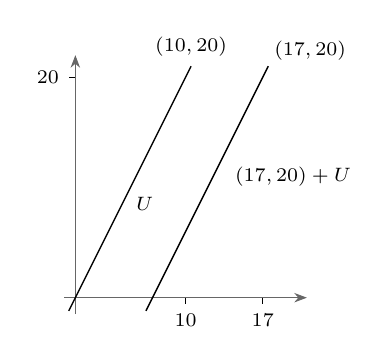
\begin{tikzpicture}[scale=.14]
  \draw[axis] (-1,0)--(21,0); \draw[axis] (0,-1.5)--(0,22);
  \draw[line width=.5pt] (-.6,-1.2)--(10.5,21) node[above,font=\scriptsize]
    {$(10,20)$};
  \draw[line width=.5pt] (6.4,-1.2)--(17.5,21) node[above right=-2pt,
    font=\scriptsize] {$(17,20)$};
  \draw (10,0)--(10,-.6) node[below,font=\scriptsize] {$10$};
  \draw (17,0)--(17,-.6) node[below,font=\scriptsize] {$17$};
  \draw (0,20)--(-.6,20) node[left,font=\scriptsize] {$20$};
  \node[font=\scriptsize] at (6.3,8.5) {$U$};
  \node[font=\scriptsize,right] at (13.6,11) {$(17,20)+U$};
\end{tikzpicture}}{$(17,20)+U$ is parallel to the subspace $U$.}%
\begin{example}[Sum of a vector and a one-dimensional subspace of
$\R^2$]\label{ax:3.96}
Suppose
\[ U = \{(x,2x)\in\R^2 : x\in\R\}. \]
Hence $U$ is the line in $\R^2$ through the origin with slope $2$. Thus
\[ (17,20)+U \]
is the line in $\R^2$ that contains the point $(17,20)$ and has slope $2$.

Because
\[ (10,20)\in U \quad\text{and}\quad (17,20)\in(17,20)+U, \]
we see that $(17,20)+U$ is obtained by moving $U$ to the right by $7$ units.
\end{example}

\begin{definition}[Translate]\label{ax:3.97}
For $v\in V$ and $U$ a subset of $V$, the set $v+U$ is said to be a
\emph{translate} of $U$.
\end{definition}

\begin{example}[Translates]\label{ax:3.98}\leavevmode
\begin{itemize}
\item If $U$ is the line in $\R^2$ defined by $U=\{(x,2x)\in\R^2 : x\in\R\}$,
  then all lines in $\R^2$ with slope $2$ are translates of $U$. See Example
  \ref{ax:3.96} above for a drawing of $U$ and one of its translates.
\item More generally, if $U$ is a line in $\R^2$, then the set of all
  translates of $U$ is the set of all lines in $\R^2$ that are parallel to $U$.
\item If $U=\{(x,y,0)\in\R^3 : x,y\in\R\}$, then the translates of $U$ are the
  planes in $\R^3$ that are parallel to the $xy$-plane $U$.
\item More generally, if $U$ is a plane in $\R^3$, then the set of all
  translates of $U$ is the set of all planes in $\R^3$ that are parallel to $U$
  (see, for example, Exercise~7).
\end{itemize}
\end{example}

\begin{definition}[Quotient space, $V/U$]\label{ax:3.99}
Suppose $U$ is a subspace of $V$. Then the \emph{quotient space} $V/U$ is the
set of all translates of $U$. Thus
\[ V/U = \{v+U : v\in V\}. \]
\end{definition}

\begin{example}[Quotient spaces]\label{ax:3.100}\leavevmode
\begin{itemize}
\item If $U=\{(x,2x)\in\R^2 : x\in\R\}$, then $\R^2/U$ is the set of all lines
  in $\R^2$ that have slope $2$.
\item If $U$ is a line in $\R^3$ containing the origin, then $\R^3/U$ is the set
  of all lines in $\R^3$ parallel to $U$.
\item If $U$ is a plane in $\R^3$ containing the origin, then $\R^3/U$ is the
  set of all planes in $\R^3$ parallel to $U$.
\end{itemize}
\end{example}

Our next goal is to make $V/U$ into a vector space. To do this, we will need
the next result.

\begin{result}[Two translates of a subspace are equal or
disjoint]\label{ax:3.101}
Suppose $U$ is a subspace of $V$ and $v,w\in V$. Then
\[ v-w\in U \iff v+U=w+U \iff (v+U)\cap(w+U)\ne\varnothing. \]
\end{result}

\begin{proof}
First suppose $v-w\in U$. If $u\in U$, then
\[ v+u = w+\bigl((v-w)+u\bigr)\in w+U. \]
Thus $v+U\subseteq w+U$. Similarly, $w+U\subseteq v+U$. Thus $v+U=w+U$,
completing the proof that $v-w\in U$ implies $v+U=w+U$.

The equation $v+U=w+U$ implies that $(v+U)\cap(w+U)\ne\varnothing$.

Now suppose $(v+U)\cap(w+U)\ne\varnothing$. Thus there exist $u_1,u_2\in U$
such that
\[ v+u_1 = w+u_2. \]
Thus $v-w=u_2-u_1$. Hence $v-w\in U$, showing that
$(v+U)\cap(w+U)\ne\varnothing$ implies $v-w\in U$, which completes the proof.
\end{proof}

Now we can define addition and scalar multiplication on $V/U$.

\begin{definition}[Addition and scalar multiplication on $V/U$]\label{ax:3.102}
Suppose $U$ is a subspace of $V$. Then \emph{addition} and \emph{scalar
multiplication} are defined on $V/U$ by
\begin{align*}
(v+U)+(w+U) &= (v+w)+U\\
\lambda(v+U) &= (\lambda v)+U
\end{align*}
for all $v,w\in V$ and all $\lambda\in\F$.
\end{definition}

As part of the proof of the next result, we will show that the definitions above
make sense.

\begin{result}[Quotient space is a vector space]\label{ax:3.103}
Suppose $U$ is a subspace of $V$. Then $V/U$, with the operations of addition
and scalar multiplication as defined above, is a vector space.
\end{result}

\begin{proof}
The potential problem with the definitions above of addition and scalar
multiplication on $V/U$ is that the representation of a translate of $U$ is not
unique. Specifically, suppose $v_1,v_2,w_1,w_2\in V$ are such that
\[ v_1+U=v_2+U \quad\text{and}\quad w_1+U=w_2+U. \]
To show that the definition of addition on $V/U$ given above makes sense, we
must show that $(v_1+w_1)+U=(v_2+w_2)+U$.

By \ref{ax:3.101}, we have
\[ v_1-v_2\in U \quad\text{and}\quad w_1-w_2\in U. \]
Because $U$ is a subspace of $V$ and thus is closed under addition, this implies
that $(v_1-v_2)+(w_1-w_2)\in U$. Thus $(v_1+w_1)-(v_2+w_2)\in U$. Using
\ref{ax:3.101} again, we see that
\[ (v_1+w_1)+U = (v_2+w_2)+U, \]
as desired. Thus the definition of addition on $V/U$ makes sense.

Similarly, suppose $\lambda\in\F$. We are still assuming that $v_1+U=v_2+U$.
Because $U$ is a subspace of $V$ and thus is closed under scalar multiplication,
we have $\lambda(v_1-v_2)\in U$. Thus $\lambda v_1-\lambda v_2\in U$. Hence
\ref{ax:3.101} implies that
\[ (\lambda v_1)+U = (\lambda v_2)+U. \]
Thus the definition of scalar multiplication on $V/U$ makes sense.

Now that addition and scalar multiplication have been defined on $V/U$, the
verification that these operations make $V/U$ into a vector space is
straightforward and is left to the reader. Note that the additive identity of
$V/U$ is $0+U$ (which equals $U$) and that the additive inverse of $v+U$ is
$(-v)+U$.
\end{proof}

The next concept will lead to a computation of the dimension of $V/U$.

\begin{definition}[Quotient map, $\pi$]\label{ax:3.104}
Suppose $U$ is a subspace of $V$. The \emph{quotient map} $\pi\colon V\to V/U$
is the linear map defined by
\[ \pi(v) = v+U \]
for each $v\in V$.
\end{definition}

The reader should verify that $\pi$ is indeed a linear map. Although $\pi$
depends on $U$ as well as $V$, these spaces are left out of the notation because
they should be clear from the context.

\begin{result}[Dimension of quotient space]\label{ax:3.105}
Suppose $V$ is finite-dimensional and $U$ is a subspace of $V$. Then
\[ \dim V/U = \dim V-\dim U. \]
\end{result}

\begin{proof}
Let $\pi$ denote the quotient map from $V$ to $V/U$. If $v\in V$, then
$v+U=0+U$ if and only if $v\in U$ (by \ref{ax:3.101}), which implies that
$\nul\pi=U$. The definition of $\pi$ implies $\range\pi=V/U$. The fundamental
theorem of linear maps (\ref{ax:3.21}) now implies $\dim V=\dim U+\dim V/U$,
which gives the desired result.
\end{proof}

Each linear map $T$ on $V$ induces a linear map $\widetilde{T}$ on
$V/(\nul T)$, as defined below.

\begin{notation}[$\widetilde{T}$]\label{ax:3.106}
Suppose $T\in\Lin(V,W)$. Define $\widetilde{T}\colon V/(\nul T)\to W$ by
\[ \widetilde{T}(v+\nul T) = Tv. \]
\end{notation}

To show that the definition of $\widetilde{T}$ makes sense, suppose $u,v\in V$
are such that $u+\nul T=v+\nul T$. By \ref{ax:3.101}, we have $u-v\in\nul T$.
Thus $T(u-v)=0$. Hence $Tu=Tv$. Thus the definition of $\widetilde{T}$ indeed
makes sense. The routine verification that $\widetilde{T}$ is a linear map from
$V/(\nul T)$ to $W$ is left to the reader.

The next result shows that we can think of $\widetilde{T}$ as a modified version
of $T$, with a domain that produces a one-to-one map.

\begin{result}[Null space and range of $\widetilde{T}$]\label{ax:3.107}
Suppose $T\in\Lin(V,W)$. Then
\begin{parts}
\item $\widetilde{T}\circ\pi=T$, where $\pi$ is the quotient map of $V$ onto
  $V/(\nul T)$;
\item $\widetilde{T}$ is injective;
\item $\range\widetilde{T}=\range T$;
\item $V/(\nul T)$ and $\range T$ are isomorphic vector spaces.
\end{parts}
\end{result}

\begin{proof}\leavevmode
\begin{parts}
\item If $v\in V$, then $(\widetilde{T}\circ\pi)(v)=\widetilde{T}\bigl(\pi(v)\bigr)
  =\widetilde{T}(v+\nul T)=Tv$, as desired.
\item Suppose $v\in V$ and $\widetilde{T}(v+\nul T)=0$. Then $Tv=0$. Thus
  $v\in\nul T$. Hence \ref{ax:3.101} implies that $v+\nul T=0+\nul T$. This
  implies that $\nul\widetilde{T}=\{0+\nul T\}$. Hence $\widetilde{T}$ is
  injective, as desired.
\item The definition of $\widetilde{T}$ shows that
  $\range\widetilde{T}=\range T$.
\item Now (b) and (c) imply that if we think of $\widetilde{T}$ as mapping into
  $\range T$, then $\widetilde{T}$ is an isomorphism from $V/(\nul T)$ onto
  $\range T$. \qedhere
\end{parts}
\end{proof}

% ------------------------------------------------------------------ exercises
\exercisesheading{3E}

\begin{exercise}
Suppose $T$ is a function from $V$ to $W$. The \emph{graph} of $T$ is the
subset of $V\times W$ defined by
\[ \text{graph of } T = \{(v,Tv)\in V\times W : v\in V\}. \]
Prove that $T$ is a linear map if and only if the graph of $T$ is a subspace of
$V\times W$.
\exnote{Formally, a function $T$ from $V$ to $W$ is a subset $T$ of $V\times W$
such that for each $v\in V$, there exists exactly one element $(v,w)\in T$. In
other words, formally a function is what is called above its graph. We do not
usually think of functions in this formal manner. However, if we do become
formal, then this exercise could be rephrased as follows: Prove that a function
$T$ from $V$ to $W$ is a linear map if and only if $T$ is a subspace of
$V\times W$.}
\end{exercise}
\begin{solution}\emergencystretch=1.5em
Let $G(T)$ denote the graph of $T$. Now, suppose $T$ is a linear map. Then
$G(T)$ is nonempty since $(0,T0)=(0,0)\in G(T)$. Now, let
$(v_1,Tv_1),(v_2,Tv_2)\in G(T)$. Then
\[ (v_1-v_2,Tv_1-Tv_2) = (v_1,Tv_1)-(v_2,Tv_2)\in G(T) \]
since $T$ is linear. Now, let $(v,Tv)\in G(T)$ and $\alpha\in\F$. Then
\[ (\alpha v,\alpha Tv) = \alpha(v,Tv)\in G(T) \]
since $T$ is linear. Thus, $G(T)$ is a subspace of $V\times W$.

Conversely, suppose $G(T)$ is a subspace of $V\times W$. By definition, we have
$(v_1,Tv_1),\allowbreak(v_2,Tv_2)\in G(T)$ for all $v_1,v_2\in V$. Since $G(T)$ is a
subspace of $V\times W$, for all $\alpha,\beta\in\F$, we have
\[ (\alpha v_1+\beta v_2,\alpha Tv_1+\beta Tv_2)
   = \alpha(v_1,Tv_1)+\beta(v_2,Tv_2)\in G(T). \]
By definition of $G(T)$, we have $\alpha Tv_1+\beta Tv_2=T(\alpha v_1+\beta
v_2)$. Thus, $T$ is a linear map.
\end{solution}

\begin{exercise}
Suppose that $V_1,\dots,V_m$ are vector spaces such that
$V_1\times\cdots\times V_m$ is finite-dimensional. Prove that $V_k$ is
finite-dimensional for each $k=1,\dots,m$.
\end{exercise}
\begin{solution}\emergencystretch=1.5em
Let $V=V_1\times\cdots\times V_m$, and consider $T\in\Lin(V,V_k)$ defined by
$T(v_1,\dots,v_m)=v_k$. Then $T$ is a linear map since for all
$\alpha,\beta\in\F$ and all $(v_1,\dots,v_m),(w_1,\dots,w_m)\in V$, we have
\begin{align*}
T\bigl(\alpha(v_1,\dots,v_m)+\beta(w_1,\dots,w_m)\bigr)
  &= T(\alpha v_1+\beta w_1,\dots,\alpha v_m+\beta w_m)\\
  &= \alpha v_k+\beta w_k\\
  &= \alpha T(v_1,\dots,v_m)+\beta T(w_1,\dots,w_m).
\end{align*}
Moreover, $T$ is surjective since for any $v_k\in V_k$, we have
$v_k=T(0,\dots,0,v_k,0,\dots,0)$ where $v_k$ is in the $k$-th coordinate. Since
$V$ is finite-dimensional and $T$ is a linear map that is surjective, it follows
that $V_k$ is finite-dimensional.
\end{solution}

\begin{exercise}
Suppose $V_1,\dots,V_m$ are vector spaces. Prove that
$\Lin(V_1\times\cdots\times V_m,W)$ and
$\Lin(V_1,W)\times\cdots\times\Lin(V_m,W)$ are isomorphic vector spaces.
\exnote{There is no assumption in the exercise above or in the two following
exercises that the vector spaces are finite-dimensional.}
\end{exercise}
\begin{solution}
Let $V=V_1\times\cdots\times V_m$. Let
$L=\Lin(V_1,W)\times\cdots\times\Lin(V_m,W)$. Define
$T\in\Lin\bigl(\Lin(V,W),L\bigr)$ by
\[ T(S) = (S\circ\iota_1,\dots,S\circ\iota_m) \]
where $\iota_k\in\Lin(V_k,V)$ is the map defined as
\[ \iota_k(v_k) = (0,\dots,0,v_k,0,\dots,0) \]
with $\iota_k(v_k)$ having $v_k$ in the $k$-th coordinate and $0$ in all other
coordinates. Then $T$ is linear since for all $\alpha,\beta\in\F$ and all
$S_1,S_2\in\Lin(V,W)$, we have
\begin{align*}
T(\alpha S_1+\beta S_2)
  &= \bigl((\alpha S_1+\beta S_2)\circ\iota_1,\dots,
     (\alpha S_1+\beta S_2)\circ\iota_m\bigr)\\
  &= \bigl(\alpha(S_1\circ\iota_1)+\beta(S_2\circ\iota_1),\dots,
     \alpha(S_1\circ\iota_m)+\beta(S_2\circ\iota_m)\bigr)\\
  &= \alpha T(S_1)+\beta T(S_2),
\end{align*}
hence $T$ is a linear map. Now suppose $T(S)=0$. Then $S\circ\iota_k=0$ for all
$k=1,\dots,m$. Moreover, for all $(v_1,\dots,v_m)\in V$, we have
\begin{align*}
S(v_1,\dots,v_m) &= S\bigl(\iota_1(v_1)+\cdots+\iota_m(v_m)\bigr)\\
  &= S\circ\iota_1(v_1)+\cdots+S\circ\iota_m(v_m) = 0.
\end{align*}
It follows that $S(v_1,\dots,v_m)=0$ for all $(v_1,\dots,v_m)\in V$. Thus,
$S=0$, and hence $T$ is injective.

Now, let $(S_1,\dots,S_m)\in L$. Define $S\in\Lin(V,W)$ by
$S(v_1,\dots,v_m)=S_1v_1+\cdots+S_mv_m$. Then $T(S)=(S_1,\dots,S_m)$. Thus, $T$
is surjective. Therefore, $T$ is an isomorphism.
\end{solution}

\begin{exercise}
Suppose $W_1,\dots,W_m$ are vector spaces. Prove that
$\Lin(V,W_1\times\cdots\times W_m)$ and
$\Lin(V,W_1)\times\cdots\times\Lin(V,W_m)$ are isomorphic vector spaces.
\end{exercise}
\begin{solution}\emergencystretch=1.5em
\solnote{Manual Remark}{Note the difference between this exercise and
Exercise~3E3. Here, the domain is decomposed, while in Exercise~3E3, the
codomain is decomposed. Hence, the use of the maps $\iota_k$ and $\pi_k$ in the
solutions to these exercises are reversed.}
Let $W=W_1\times\cdots\times W_m$. Let
$L=\Lin(V,W_1)\times\cdots\times\Lin(V,W_m)$. Define
$T\in\Lin\bigl(\Lin(V,W),L\bigr)$ by
\[ T(S) = (\pi_1\circ S,\dots,\pi_m\circ S) \]
where $\pi_k\in\Lin(W,W_k)$ is the map defined as
\[ \pi_k(w_1,\dots,w_m) = w_k \]
Then $T$ is linear since for all $\alpha,\beta\in\F$ and all
$S_1,S_2\in\Lin(V,W)$, we have
\begin{align*}
T(\alpha S_1+\beta S_2)
  &= \bigl(\pi_1\circ(\alpha S_1+\beta S_2),\dots,
     \pi_m\circ(\alpha S_1+\beta S_2)\bigr)\\
  &= \bigl(\alpha(\pi_1\circ S_1)+\beta(\pi_1\circ S_2),\dots,
     \alpha(\pi_m\circ S_1)+\beta(\pi_m\circ S_2)\bigr)\\
  &= \alpha T(S_1)+\beta T(S_2),
\end{align*}
hence $T$ is a linear map. Now suppose $T(S)=0$. Then $\pi_k\circ S=0$ for all
$k=1,\dots,m$. Moreover, for all $v\in V$, we have
\[ Sv = \bigl(\pi_1(Sv),\dots,\pi_m(Sv)\bigr) = (0,\dots,0) = 0. \]
It follows that $Sv=0$ for all $v$, hence $S=0$, and thus $T$ is injective.

Now let $(S_1,\dots,S_m)\in L$. Define $S\in\Lin(V,W)$ by
$Sv=(S_1v,\dots,S_mv)$. Then $T(S)=(S_1,\dots,S_m)$. Thus, $T$ is surjective.
Therefore, $T$ is an isomorphism.
\end{solution}

\begin{exercise}
For $m$ a positive integer, define $V^m$ by
\[ V^m = \ftimes{V\times\cdots\times V}{m\text{ times}}. \]
Prove that $V^m$ and $\Lin(\F^m,V)$ are isomorphic vector spaces.
\end{exercise}
\begin{solution}\emergencystretch=1.5em
Let $e_1,\dots,e_m$ be the standard basis of $\F^m$. Define
$T\in\Lin\bigl(V^m,\allowbreak\Lin(\F^m,V)\bigr)$ by
\[ T(v_1,\dots,v_m)(\lambda_1,\dots,\lambda_m)
   = \lambda_1v_1+\cdots+\lambda_mv_m. \]
Then $T$ is linear since for all $\alpha,\beta\in\F$ and all
$v=(v_1,\dots,v_m),w=(w_1,\dots,w_m)\in V^m$, we have
\begin{align*}
T(\alpha v+\beta w)(\lambda_1,\dots,\lambda_m)
  &= T(\alpha v_1+\beta w_1,\dots,\alpha v_m+\beta w_m)
     (\lambda_1,\dots,\lambda_m)\\
  &= \lambda_1(\alpha v_1+\beta w_1)+\cdots+\lambda_m(\alpha v_m+\beta w_m)\\
  &= \alpha(\lambda_1v_1+\cdots+\lambda_mv_m)
     +\beta(\lambda_1w_1+\cdots+\lambda_mw_m)\\
  &= \alpha T(v)(\lambda_1,\dots,\lambda_m)
     +\beta T(w)(\lambda_1,\dots,\lambda_m),
\end{align*}
hence $T$ is a linear map. Now suppose $T(v)=0$. Then $T(v)(e_k)=0$ for all
$k=1,\dots,m$. It follows that $v_k=0$ for all $k=1,\dots,m$, hence $v=0$, and
thus $T$ is injective.

Now let $S\in\Lin(\F^m,V)$. Define $v\in V^m$ by $v_k=Se_k$ for all
$k=1,\dots,m$. Then $T(v)=S$. Thus, $T$ is surjective. Therefore, $T$ is an
isomorphism.
\end{solution}

\begin{exercise}
Suppose that $v,x$ are vectors in $V$ and that $U,W$ are subspaces of $V$ such
that $v+U=x+W$. Prove that $U=W$.
\end{exercise}
\begin{solution}
Let $u\in U$. Then $v+u\in v+U=x+W$. Thus, there exists $w\in W$ such that
$v+u=x+w$. Note that $v\in x+W$ implies the existence of some $w'\in W$ such
that $v=x+w'$, or $x-v=-w'\in W$. Similarly, $x\in v+U$ implies the existence of
some $u'\in U$ such that $x=v+u'$, or $v-x=-u'\in U$. It follows that
$u=(x-v)+w\in W$, hence $U\subseteq W$. Now let $w\in W$. Then
$x+w\in x+W=v+U$. Thus, there exists $u\in U$ such that $x+w=v+u$. It follows
that $w=(v-x)+u\in U$, hence $W\subseteq U$. Therefore, $U=W$.
\end{solution}

\begin{exercise}
Let $U=\{(x,y,z)\in\R^3 : 2x+3y+5z=0\}$. Suppose $A\subseteq\R^3$. Prove that
$A$ is a translate of $U$ if and only if there exists $c\in\R$ such that
\[ A = \{(x,y,z)\in\R^3 : 2x+3y+5z=c\}. \]
\end{exercise}
\begin{solution}
Suppose $A$ is a translate of $U$. Then there exists $v\in\R^3$ such that
$A=v+U$. Let $v=(x_0,y_0,z_0)$. Then
\begin{align*}
A &= v+U\\
  &= \{(x_0,y_0,z_0)+(x,y,z)\in\R^3 \mid 2x+3y+5z=0\}\\
  &= \{(x',y',z')\in\R^3 \mid 2(x'-x_0)+3(y'-y_0)+5(z'-z_0)=0\}\\
  &= \{(x',y',z')\in\R^3 \mid 2x'+3y'+5z'=2x_0+3y_0+5z_0\}.
\end{align*}
Conversely, suppose there exists $c\in\R$ such that
\[ A = \{(x,y,z)\in\R^3 \mid 2x+3y+5z=c\}. \]
Let $v=(x_0,y_0,z_0)$ where $x_0,y_0,z_0$ are any real numbers such that
$2x_0+3y_0+5z_0=c$. Then
\begin{align*}
v+U &= (x_0,y_0,z_0)+U\\
    &= \{(x_0,y_0,z_0)+(x,y,z)\in\R^3 \mid 2x+3y+5z=0\}\\
    &= A. \qedhere
\end{align*}
\end{solution}

\begin{exercise}\leavevmode
\begin{parts}
\item Suppose $T\in\Lin(V,W)$ and $c\in W$. Prove that $\{x\in V : Tx=c\}$ is
  either the empty set or is a translate of $\nul T$.
\item Explain why the set of solutions to a system of linear equations such as
  \ref{ax:3.27} is either the empty set or is a translate of some subspace of
  $\F^n$.
\end{parts}
\end{exercise}
\begin{solution}\leavevmode
\begin{parts}
\item Suppose $T\in\Lin(V,W)$ and $c\in W$. Let $A=\{x\in V \mid Tx=c\}$. If $A$
  is nonempty, then there exists $v\in V$ such that $Tv=c$. We claim that
  $A=v+\nul T$. Let $x\in A$. Then $Tx=c=Tv$, hence $T(x-v)=0$, and thus
  $x-v\in\nul T$. It follows that $x\in v+\nul T$, hence $A\subseteq v+\nul T$.
  Now let $y\in v+\nul T$. Then there exists $u\in\nul T$ such that $y=v+u$. It
  follows that $Ty=T(v+u)=Tv+Tu=c+0=c$, hence $y\in A$, and thus
  $v+\nul T\subseteq A$. Therefore, $A=v+\nul T$.
\item A system of linear equations such as \ref{ax:3.27} can be written in the
  form $Tx=c$ for some linear map $T$ and some vector $c$. By part (a), the set
  of solutions to this system of linear equations is either the empty set or is
  a translate of $\nul T$, which is a subspace of $\F^n$. \qedhere
\end{parts}
\end{solution}

\begin{exercise}
Prove that a nonempty subset $A$ of $V$ is a translate of some subspace of $V$
if and only if $\lambda v+(1-\lambda)w\in A$ for all $v,w\in A$ and all
$\lambda\in\F$.
\end{exercise}
\begin{solution}
Suppose $A$ is a translate of some subspace of $V$. Then there exists $v\in V$
and a subspace $U$ of $V$ such that $A=v+U$. Let $v+u,v+u'\in A$. Then for any
$\lambda\in\F$,
\[ \lambda(v+u)+(1-\lambda)(v+u')
   = v+\underbrace{\bigl(\lambda u+(1-\lambda)u'\bigr)}_{\in U}\in A. \]
Conversely, suppose $\lambda v+(1-\lambda)w\in A$ for all $v,w\in A$ and all
$\lambda\in\F$. Fix some $v_0\in A$, and let $U=\{u\in V \mid v_0+u\in A\}$. We
first claim that $U$ is a subspace of $V$. Since $v_0=v_0+0\in A$, we have
$0\in U$. Let $u_1,u_2\in U$. Then $v_0+u_1,v_0+u_2\in A$. Now let
$\lambda\in\F$. Then
\begin{align*}
\lambda(v_0+u_1)+(1-\lambda)(v_0+u_2) &= v_0+\lambda u_1+(1-\lambda)u_2\\
  &= v_0+\bigl(\lambda u_1+(1-\lambda)u_2\bigr)\in A.
\end{align*}
It follows that $\lambda u_1+(1-\lambda)u_2\in U$, hence $U$ is a subspace of
$V$. Now we claim that $A=v_0+U$. Let $w\in A$. By definition,
$v_0+(w-v_0)=w\in A$, hence $w-v_0\in U$, and thus $w\in v_0+U$, so
$A\subseteq v_0+U$. Now let $v_0+u\in v_0+U$. Then $v_0+u\in A$ by definition of
$U$, hence $v_0+U\subseteq A$. Therefore, $A=v_0+U$.
\end{solution}

\begin{exercise}
Suppose $A_1=v+U_1$ and $A_2=w+U_2$ for some $v,w\in V$ and some subspaces
$U_1,U_2$ of $V$. Prove that the intersection $A_1\cap A_2$ is either a
translate of some subspace of $V$ or is the empty set.
\end{exercise}
\begin{solution}
If $A_1\cap A_2$ is the empty set, then we are done. Suppose that $A_1\cap A_2$
is nonempty. Let $x,y\in A_1\cap A_2$ and $\lambda\in\F$. Then $x,y\in A_1$,
hence $\lambda x+(1-\lambda)y\in A_1$. Moreover, $x,y\in A_2$, hence
$\lambda x+(1-\lambda)y\in A_2$. It follows that
$\lambda x+(1-\lambda)y\in A_1\cap A_2$. Thus, by Exercise~3E9, $A_1\cap A_2$ is
a translate of some subspace of $V$.
\end{solution}

\begin{exercise}
Suppose $U=\{(x_1,x_2,\dots)\in\F^\infty : x_k\ne0 \text{ for only finitely many
} k\}$.
\begin{parts}
\item Show that $U$ is a subspace of $\F^\infty$.
\item Prove that $\F^\infty/U$ is infinite-dimensional.
\end{parts}
\end{exercise}
\begin{solution}\emergencystretch=1.5em
\solnote{Appendix}{See the alternate proof at the end of this solution for a
generalization of this treatment, so long as you are comfortable with the idea
$\N$ can be partitioned into infinitely many disjoint infinite sets.}
\begin{parts}
\item We claim that $U$ can be reformulated as the set of vectors
  $(x_1,x_2,\dots)\in\F^\infty$ such that there exists an index $N$ such that
  $x_k=0$ for all $k>N$. To see this, suppose $(x_1,x_2,\dots)\in U$. Then there
  exists a finite set of indices $K$ such that $x_k=0$ for all $k\notin K$. If
  $K$ is empty, let $N=0$. Otherwise, let $N=\max K$. Then $x_k=0$ for all
  $k>N$.

  Conversely, suppose there exists an index $N$ such that $x_k=0$ for all
  $k>N$. Then the set of indices $\{1,2,\dots,N\}$ is finite and contains all
  indices where $x_k\ne0$, hence $(x_1,x_2,\dots)\in U$. Thus, the two
  formulations of $U$ are equivalent.

  We now show that $U$ is a subspace of $\F^\infty$. First, note that the zero
  vector $(0,0,\dots)\in U$ since it has no nonzero coordinates. Now let
  $u=(u_1,u_2,\dots),v=(v_1,v_2,\dots)\in U$. Then there exist indices $N_u$ and
  $N_v$ such that $u_k=0$ for all $k>N_u$ and $v_k=0$ for all $k>N_v$. Let
  $N=\max(N_u,N_v)$. Then for all $k>N$, we have $u_k=0$ and $v_k=0$, hence
  $(u+v)_k=u_k+v_k=0+0=0$. Thus, $u+v\in U$. Now let $\alpha\in\F$. Then for all
  $k>N_u$, we have $(\alpha u)_k=\alpha u_k=\alpha\cdot0=0$, hence
  $\alpha u\in U$. Therefore, $U$ is a subspace of $\F^\infty$.
\item For any given positive integer $m$, define the sets $B_i$ for
  $1\le i\le m$ as follows:
  \[ B_i = \{i+km \mid k\in\N\} = \{i,i+m,i+2m,\dots\}. \]
  Then $B_1,\dots,B_m$ are pairwise disjoint subsets of $\N$. For each
  $i=1,\dots,m$, define
  \[ v_i = (v_{i,1},v_{i,2},\dots)\in\F^\infty \]
  such that $v_{i,j}=1$ if $j\in B_i$ and $v_{i,j}=0$ otherwise. We claim that
  $v_1+U,\dots,v_m+U$ are linearly independent in $\F^\infty/U$.

  Let $\lambda_1,\dots,\lambda_m\in\F$ such that
  $\lambda_1(v_1+U)+\cdots+\lambda_m(v_m+U)=U$. Then
  $\lambda_1v_1+\cdots+\lambda_mv_m\in U$. Then we can show that $\lambda_i=0$
  for all $i=1,\dots,m$ as follows. For each $i$, consider the $j$-th coordinate
  of $v_i$ for $j\in B_i$. Since $v_i$ has $1$'s in all coordinates indexed by
  $B_i$ and $0$'s elsewhere, and $B_i$ is disjoint from $B_k$ for $k\ne i$, the
  $j$-th coordinate of $\lambda_1v_1+\cdots+\lambda_mv_m$ is $\lambda_i$. But
  this sum is in $U$, which means it has only finitely many nonzero coordinates.
  Since $B_i$ is infinite, it follows that $\lambda_i=0$. Hence, all
  $\lambda_i=0$, proving that $v_1+U,\dots,v_m+U$ are linearly independent.
  Since $m$ was arbitrary, $\F^\infty/U$ is infinite-dimensional.
\end{parts}

\emph{Alternate proof.}
\begin{parts}
\item Since $(0,0,\dots)\in U$, $U$ is nonempty. Suppose $x,y\in U$ and
  $c\in\F$. Let $S_x$ and $S_y$ be the sets of indices where $x$ and $y$ have
  nonzero terms, respectively. By definition, $S_x$ and $S_y$ are finite.
  $cx+y$ can only have nonzero terms at indices in $S_x\cup S_y$. Since the
  union of two finite sets is finite, $cx+y\in U$, which makes $U$ a subspace
  of $\F^\infty$.
\item Partition $\Z^+$ into a countably infinite family of disjoint infinite
  subsets $A_1,\allowbreak A_2,\allowbreak\dots$. For each $n$, define $v_n\in\F^\infty$ such that its
  $j$-th term is $1$ if $j\in A_n$ and $0$ otherwise.

  Suppose that $\sum_{i=1}^m c_i(v_i+U)=0+U$ for some positive integer $m$ and
  scalars $c_1,\dots,c_m\in\F$. Then, $w=\sum_{i=1}^m c_iv_i\in U$. By
  construction, for $i\in\{1,\dots,m\}$, the $j$-th term of $w$ is $c_i$ for all
  $j\in A_i$. Since $w\in U$, it only has a finite number of nonzero terms. But
  each $A_i$ is infinite, so this forces $c_i=0$ for all $i\in\{1,\dots,m\}$.
  Hence, $v_1+U,v_2+U,\dots$ are linearly independent in $\F^\infty/U$.

  Because $\F^\infty/U$ contains an infinite sequence of linearly independent
  vectors, it is infinite-dimensional.
\end{parts}
\end{solution}

\begin{exercise}
Suppose $v_1,\dots,v_m\in V$. Let
\[ A = \{\lambda_1v_1+\cdots+\lambda_mv_m : \lambda_1,\dots,\lambda_m\in\F
   \text{ and } \lambda_1+\cdots+\lambda_m=1\}. \]
\begin{parts}
\item Prove that $A$ is a translate of some subspace of $V$.
\item Prove that if $B$ is a translate of some subspace of $V$ and
  $\{v_1,\dots,v_m\}\subseteq B$, then $A\subseteq B$.
\item Prove that $A$ is a translate of some subspace of $V$ of dimension less
  than $m$.
\end{parts}
\end{exercise}
\begin{solution}\leavevmode
\begin{parts}
\item For any element $\lambda_1v_1+\cdots+\lambda_mv_m\in A$, we can write
  \begin{align*}
  \lambda_1v_1+\cdots+\lambda_mv_m
    &= v_1+\lambda_2(v_2-v_1)+\cdots+\lambda_m(v_m-v_1)\\
    &= v_1+\sum_{i=2}^m\lambda_i(v_i-v_1),
  \end{align*}
  where $\lambda_1=1-(\lambda_2+\cdots+\lambda_m)$. Let
  $U=\spn(v_2-v_1,\dots,v_m-v_1)$. Then $A=v_1+U$, hence $A$ is a translate of
  the subspace $U$ of $V$.
\item By Exercise~3E9, since $B$ is a translate of some subspace of $V$, we have
  $\lambda v+(1-\lambda)w\in B$ for all $v,w\in B$ and all $\lambda\in\F$. Since
  $\{v_1,\dots,v_m\}\subseteq B$, it follows that any linear combination of
  $v_1,\dots,v_m$ with coefficients summing to $1$ is in $B$. Hence,
  $A\subseteq B$.
\item The subspace $U=\spn(v_2-v_1,\dots,v_m-v_1)$ has dimension at most $m-1$,
  since it is spanned by $m-1$ vectors. Therefore, $A=v_1+U$ is a translate of a
  subspace of $V$ of dimension less than $m$. \qedhere
\end{parts}
\end{solution}

\begin{exercise}
Suppose $U$ is a subspace of $V$ such that $V/U$ is finite-dimensional. Prove
that $V$ is isomorphic to $U\times(V/U)$.
\end{exercise}
\begin{solution}
Since $V/U$ is finite-dimensional, let $v_1+U,\dots,v_m+U$ be a basis of $V/U$.
Let $W=\spn(v_1,\dots,v_m)$. We show that $V=U\oplus W$. First, note that any
$v\in V$ can be written as $v=u+w$ for some $u\in U$ and $w\in W$. Indeed, since
$v+U\in V/U$, we can write
\[ v+U = \lambda_1(v_1+U)+\cdots+\lambda_m(v_m+U) \]
for some scalars $\lambda_1,\dots,\lambda_m$. This gives
\[ v-(\lambda_1v_1+\cdots+\lambda_mv_m)\in U. \]
So setting $u=v-(\lambda_1v_1+\cdots+\lambda_mv_m)\in U$ and
$w=\lambda_1v_1+\cdots+\lambda_mv_m\in W$, we have $v=u+w$. To see that the sum
is direct, suppose $u+w=0$ with $u\in U$ and $w\in W$. Then $w=-u\in W\cap U$.
Since $w\in W$, we can write $w=\lambda_1v_1+\cdots+\lambda_mv_m$ for some
scalars $\lambda_1,\dots,\lambda_m$. Since we established that $w\in U$, we have
$w+U=0+U$. But $v_1+U,\dots,v_m+U$ are linearly independent in $V/U$, hence
$\lambda_1=\cdots=\lambda_m=0$, and thus $w=0$. It follows that $u=0$ as well,
proving that the sum is direct. Therefore, $V=U\oplus W$.

Consider the map $T\colon V\to U\times(V/U)$ given by $Tv=(u,v+U)$, where
$v=u+w$ with $u\in U$ and $w\in W$. This map is well-defined because the
decomposition $v=u+w$ is unique. It is linear, injective, and surjective, hence
an isomorphism. Therefore, $V\cong U\times(V/U)$.
\end{solution}

\begin{exercise}
Suppose $U$ and $W$ are subspaces of $V$ and $V=U\oplus W$. Suppose
$w_1,\dots,w_m$ is a basis of $W$. Prove that $w_1+U,\dots,w_m+U$ is a basis of
$V/U$.
\end{exercise}
\begin{solution}
Since $V=U\oplus W$, every $v\in V$ can be written uniquely as $v=u+w$ with
$u\in U$ and $w\in W$. We claim that $w_1+U,\dots,w_m+U$ is a basis of $V/U$.
First, we show that they span $V/U$. Let $v+U\in V/U$. Write $v=u+w$ with
$u\in U$ and $w\in W$. Then $v+U=(u+w)+U=w+U$. Since $w\in W$, we can write
$w=\lambda_1w_1+\cdots+\lambda_mw_m$ for some scalars
$\lambda_1,\dots,\lambda_m$. Hence,
$v+U=\lambda_1(w_1+U)+\cdots+\lambda_m(w_m+U)$, showing that
$w_1+U,\dots,w_m+U$ span $V/U$.

Next, we show linear independence. Suppose
$\lambda_1(w_1+U)+\cdots+\lambda_m(w_m+U)=0+U$. Then
$\lambda_1w_1+\cdots+\lambda_mw_m\in U$. But
$\lambda_1w_1+\cdots+\lambda_mw_m\in W$ and $U\cap W=\{0\}$, so
$\lambda_1w_1+\cdots+\lambda_mw_m=0$. Since $w_1,\dots,w_m$ are linearly
independent, we have $\lambda_1=\cdots=\lambda_m=0$. Therefore,
$w_1+U,\dots,w_m+U$ are linearly independent, and hence form a basis of $V/U$.
\end{solution}

\begin{exercise}
Suppose $U$ is a subspace of $V$ and $v_1+U,\dots,v_m+U$ is a basis of $V/U$
and $u_1,\dots,u_n$ is a basis of $U$. Prove that
$v_1,\dots,v_m,u_1,\dots,u_n$ is a basis of $V$.
\end{exercise}
\begin{solution}
First, we show that $v_1,\dots,v_m,u_1,\dots,u_n$ span $V$. Let $v\in V$. Then
$v+U\in V/U$, so we can write
\[ v+U = \lambda_1(v_1+U)+\cdots+\lambda_m(v_m+U) \]
for some scalars $\lambda_1,\dots,\lambda_m$. This gives
$v-(\lambda_1v_1+\cdots+\lambda_mv_m)\in U$. Since $u_1,\dots,u_n$ is a basis
of $U$, we can write $v-(\lambda_1v_1+\cdots+\lambda_mv_m)=\mu_1u_1+\cdots
+\mu_nu_n$ for some scalars $\mu_1,\dots,\mu_n$. Hence,
$v=\lambda_1v_1+\cdots+\lambda_mv_m+\mu_1u_1+\cdots+\mu_nu_n$, showing that
$v_1,\dots,v_m,u_1,\dots,u_n$ span $V$.

Next, we show linear independence. Suppose
$\lambda_1v_1+\cdots+\lambda_mv_m+\mu_1u_1+\cdots+\mu_nu_n=0$. Then
$\lambda_1v_1+\cdots+\lambda_mv_m\in U$. Then
\[ \lambda_1(v_1+U)+\cdots+\lambda_m(v_m+U) = 0+U. \]
Since $v_1+U,\dots,v_m+U$ are linearly independent in $V/U$, we must have
$\lambda_1=\cdots=\lambda_m=0$. Then the original equation reduces to
$\mu_1u_1+\cdots+\mu_nu_n=0$, and since $u_1,\dots,u_n$ are linearly
independent, we have $\mu_1=\cdots=\mu_n=0$. Therefore,
$v_1,\dots,v_m,u_1,\dots,u_n$ are linearly independent, and hence form a basis
of $V$.
\end{solution}

\begin{exercise}
Suppose $\varphi\in\Lin(V,\F)$ and $\varphi\ne0$. Prove that
$\dim V/(\nul\varphi)=1$.
\end{exercise}
\begin{solution}
From \ref{ax:3.107} in the text, we know that $V/\nul\varphi\cong\range\varphi$.
Since $\varphi\ne0$, we have $\range\varphi\ne\{0\}$, and since $\range\varphi$
is a subspace of $\F$, it follows that $\dim\range\varphi=1$. This implies
$\range\varphi=\F$, and hence $\dim V/(\nul\varphi)=\dim\range\varphi=1$.
\end{solution}

\begin{exercise}
Suppose $U$ is a subspace of $V$ such that $\dim V/U=1$. Prove that there exists
$\varphi\in\Lin(V,\F)$ such that $\nul\varphi=U$.
\end{exercise}
\begin{solution}
Since $\dim V/U=\dim\F=1$, there exists some isomorphism
$\psi\in\Lin(V/U,\F)$. Let $\pi\colon V\to V/U$ be the quotient map. Define
$\varphi=\psi\circ\pi\in\Lin(V,\F)$. Suppose $\varphi(v)=0$. Then
$\psi\bigl(\pi(v)\bigr)=0$, which implies $\pi(v)=0$ since $\psi$ is an
isomorphism. Hence, $v\in U$, and we have $\nul\varphi\subseteq U$. Conversely,
if $v\in U$, then $\pi(v)=0$, so $\varphi(v)=\psi\bigl(\pi(v)\bigr)=0$.
Therefore, $\nul\varphi=U$.
\end{solution}

\begin{exercise}
Suppose that $U$ is a subspace of $V$ such that $V/U$ is finite-dimensional.
\begin{parts}
\item Show that if $W$ is a finite-dimensional subspace of $V$ and $V=U+W$, then
  $\dim W\ge\dim V/U$.
\item Prove that there exists a finite-dimensional subspace $W$ of $V$ such that
  $\dim W=\dim V/U$ and $V=U\oplus W$.
\end{parts}
\end{exercise}
\begin{solution}\leavevmode
\begin{parts}
\item Suppose $W$ is a finite-dimensional subspace of $V$ and $V=U+W$. Let
  $\pi\colon V\to V/U$ be the quotient map, and consider the restriction
  $\pi|_W\colon W\to V/U$. To see that $\range(\pi|_W)=V/U$, note that for any
  $v+U\in V/U$, we can write $v=u+w$ for some $u\in U$ and $w\in W$. Then
  $\pi(v)=\pi(u+w)=\pi(u)+\pi(w)=0+\pi(w)=\pi(w)$, so
  $v+U=\pi(w)\in\range(\pi|_W)$. Hence, $\range(\pi|_W)=V/U$. From the
  fundamental theorem of linear maps, we have
  \begin{align*}
  \dim W &= \dim\nul\pi|_W+\dim\range(\pi|_W)\\
         &= \dim\nul\pi|_W+\dim V/U \ge \dim V/U.
  \end{align*}
\item Let $v_1+U,\dots,v_m+U$ be a basis of $V/U$. We claim that
  $v_1,\dots,v_m$ are linearly independent. Suppose
  $\lambda_1v_1+\cdots+\lambda_mv_m=0$ for some scalars
  $\lambda_1,\dots,\lambda_m$. Then
  \[ \lambda_1v_1+\cdots+\lambda_mv_m\in U. \]
  But $\lambda_1(v_1+U)+\cdots+\lambda_m(v_m+U)=0$ in $V/U$, and since
  $v_1+U,\dots,v_m+U$ are linearly independent, it follows that
  $\lambda_1=\cdots=\lambda_m=0$. Hence, $v_1,\dots,v_m$ are linearly
  independent.

  Let $W=\spn\{v_1,\dots,v_m\}$. Then $\dim W=m=\dim V/U$. For any $v\in V$, we
  can write
  \[ v+U = \lambda_1(v_1+U)+\cdots+\lambda_m(v_m+U). \]
  This implies that
  \[ v-(\lambda_1v_1+\cdots+\lambda_mv_m)\in U, \]
  so $v\in U+W$. Hence, $V=U+W$. To see that $U\cap W=\{0\}$, let
  $w\in U\cap W$. Then $w\in W$, so $w=\lambda_1v_1+\cdots+\lambda_mv_m$ for
  some scalars $\lambda_1,\dots,\lambda_m$. But $w\in U$, so $w+U=0$ in $V/U$.
  Hence,
  \[ \lambda_1(v_1+U)+\cdots+\lambda_m(v_m+U) = 0 \]
  in $V/U$. Since $v_1+U,\dots,v_m+U$ are linearly independent, it follows that
  $\lambda_1=\cdots=\lambda_m=0$. Hence, $w=0$, and we have $U\cap W=\{0\}$.
  Therefore, $V=U\oplus W$. \qedhere
\end{parts}
\end{solution}

\begin{exercise}
Suppose $T\in\Lin(V,W)$ and $U$ is a subspace of $V$. Let $\pi$ denote the
quotient map from $V$ onto $V/U$. Prove that there exists $S\in\Lin(V/U,W)$ such
that $T=S\circ\pi$ if and only if $U\subseteq\nul T$.
\end{exercise}
\begin{solution}
Suppose $S\in\Lin(V/U,W)$ is such that $T=S\circ\pi$. Then for any $u\in U$, we
have $T(u)=S\bigl(\pi(u)\bigr)=S(0)=0$, so $U\subseteq\nul T$.

Conversely, suppose $U\subseteq\nul T$. Define $S\colon V/U\to W$ by
$S(v+U)=T(v)$. This is well-defined because if $v+U=v'+U$, then
$v-v'\in U\subseteq\nul T$, so $T(v)=T(v')$. It is straightforward to check that
$S$ is linear and that $T=S\circ\pi$.
\end{solution}

\iftestbuild % TEST-ONLY-BEGIN
\setcounter{section}{5}\setcounter{theorem}{107}
\fi % TEST-ONLY-END
% Source: book pp. 105--118 (PDF 119--132); solutions pp. 113--128, 172--173.
% A short note set in small italics under an exercise, as Axler does.
\section{Duality}

\subsection{Dual Space and Dual Map}

Linear maps into the scalar field $\F$ play a special role in linear algebra, and
thus they get a special name.

\begin{definition}[Linear functional]\label{ax:3.108}
A \emph{linear functional} on $V$ is a linear map from $V$ to $\F$. In other
words, a linear functional is an element of $\Lin(V,\F)$.
\end{definition}

\begin{example}[Linear functionals]\label{ax:3.109}\leavevmode
\begin{itemize}
\item Define $\varphi\colon\R^3\to\R$ by $\varphi(x,y,z)=4x-5y+2z$. Then
  $\varphi$ is a linear functional on $\R^3$.
\item Fix $(c_1,\dots,c_n)\in\F^n$. Define $\varphi\colon\F^n\to\F$ by
  $\varphi(x_1,\dots,x_n)=c_1x_1+\cdots+c_nx_n$. Then $\varphi$ is a linear
  functional on $\F^n$.
\item Define $\varphi\colon\Poly(\R)\to\R$ by
  \[ \varphi(p) = 3p''(5)+7p(4). \]
  Then $\varphi$ is a linear functional on $\Poly(\R)$.
\item Define $\varphi\colon\Poly(\R)\to\R$ by
  \[ \varphi(p) = \int_0^1 p \]
  for each $p\in\Poly(\R)$. Then $\varphi$ is a linear functional on
  $\Poly(\R)$.
\end{itemize}
\end{example}

The vector space $\Lin(V,\F)$ also gets a special name and special notation.

\begin{definition}[Dual space, $V'$]\label{ax:3.110}
The \emph{dual space} of $V$, denoted by $V'$, is the vector space of all linear
functionals on $V$. In other words, $V'=\Lin(V,\F)$.
\end{definition}

\begin{result}[$\dim V'=\dim V$]\label{ax:3.111}
Suppose $V$ is finite-dimensional. Then $V'$ is also finite-dimensional and
\[ \dim V' = \dim V. \]
\end{result}

\begin{proof}
By \ref{ax:3.72} we have
\[ \dim V' = \dim\Lin(V,\F) = (\dim V)(\dim\F) = \dim V, \]
as desired.
\end{proof}

In the following definition, the linear map lemma (\ref{ax:3.4}) implies that
each $\varphi_j$ is well defined.

\begin{definition}[Dual basis]\label{ax:3.112}
If $v_1,\dots,v_n$ is a basis of $V$, then the \emph{dual basis} of
$v_1,\dots,v_n$ is the list $\varphi_1,\dots,\varphi_n$ of elements of $V'$,
where each $\varphi_j$ is the linear functional on $V$ such that
\[ \varphi_j(v_k) = \begin{cases} 1 & \text{if } k=j,\\
                                 0 & \text{if } k\ne j. \end{cases} \]
\end{definition}

\begin{example}[The dual basis of the standard basis of $\F^n$]\label{ax:3.113}
Suppose $n$ is a positive integer. For $1\le j\le n$, define $\varphi_j$ to be
the linear functional on $\F^n$ that selects the $j^{\text{th}}$ coordinate of a
vector in $\F^n$. Thus
\[ \varphi_j(x_1,\dots,x_n) = x_j \]
for each $(x_1,\dots,x_n)\in\F^n$.

Let $e_1,\dots,e_n$ be the standard basis of $\F^n$. Then
\[ \varphi_j(e_k) = \begin{cases} 1 & \text{if } k=j,\\
                                 0 & \text{if } k\ne j. \end{cases} \]
Thus $\varphi_1,\dots,\varphi_n$ is the dual basis of the standard basis
$e_1,\dots,e_n$ of $\F^n$.
\end{example}

The next result shows that the dual basis of a basis of $V$ consists of the
linear functionals on $V$ that give the coefficients for expressing a vector in
$V$ as a linear combination of the basis vectors.

\begin{result}[Dual basis gives coefficients for linear combination]\label{ax:3.114}
Suppose $v_1,\dots,v_n$ is a basis of $V$ and $\varphi_1,\dots,\varphi_n$ is the
dual basis. Then
\[ v = \varphi_1(v)v_1+\cdots+\varphi_n(v)v_n \]
for each $v\in V$.
\end{result}

\begin{proof}
Suppose $v\in V$. Then there exist $c_1,\dots,c_n\in\F$ such
that\refstepcounter{theorem}
\begin{equation*}
v = c_1v_1+\cdots+c_nv_n. \tag*{\thetheorem}\label{ax:3.115}
\end{equation*}
If $j\in\{1,\dots,n\}$, then applying $\varphi_j$ to both sides of the equation
above gives
\[ \varphi_j(v) = c_j. \]
Substituting the values for $c_1,\dots,c_n$ given by the equation above into
\ref{ax:3.115} shows that $v=\varphi_1(v)v_1+\cdots+\varphi_n(v)v_n$.
\end{proof}

The next result shows that the dual basis is indeed a basis of the dual space.
Thus the terminology ``dual basis'' is justified.

\begin{result}[Dual basis is a basis of the dual space]\label{ax:3.116}
Suppose $V$ is finite-dimensional. Then the dual basis of a basis of $V$ is a
basis of $V'$.
\end{result}

\begin{proof}
Suppose $v_1,\dots,v_n$ is a basis of $V$. Let $\varphi_1,\dots,\varphi_n$ denote
the dual basis.

To show that $\varphi_1,\dots,\varphi_n$ is a linearly independent list of
elements of $V'$, suppose $a_1,\dots,a_n\in\F$ are such
that\refstepcounter{theorem}
\begin{equation*}
a_1\varphi_1+\cdots+a_n\varphi_n = 0. \tag*{\thetheorem}\label{ax:3.117}
\end{equation*}
Now
\[ (a_1\varphi_1+\cdots+a_n\varphi_n)(v_k) = a_k \]
for each $k=1,\dots,n$. Thus \ref{ax:3.117} shows that $a_1=\cdots=a_n=0$. Hence
$\varphi_1,\dots,\varphi_n$ is linearly independent.

Because $\varphi_1,\dots,\varphi_n$ is a linearly independent list in $V'$ whose
length equals $\dim V'$ (by \ref{ax:3.111}), we can conclude that
$\varphi_1,\dots,\varphi_n$ is a basis of $V'$ (see \ref{ax:2.38}).
\end{proof}

In the definition below, note that if $T$ is a linear map from $V$ to $W$ then
$T'$ is a linear map from $W'$ to $V'$.

\begin{definition}[Dual map, $T'$]\label{ax:3.118}
Suppose $T\in\Lin(V,W)$. The \emph{dual map} of $T$ is the linear map
$T'\in\Lin(W',V')$ defined for each $\varphi\in W'$ by
\[ T'(\varphi) = \varphi\circ T. \]
\end{definition}

If $T\in\Lin(V,W)$ and $\varphi\in W'$, then $T'(\varphi)$ is defined above to be
the composition of the linear maps $\varphi$ and $T$. Thus $T'(\varphi)$ is
indeed a linear map from $V$ to $\F$; in other words, $T'(\varphi)\in V'$.

The following two bullet points show that $T'$ is a linear map from $W'$ to
$V'$.
\begin{itemize}
\item If $\varphi,\psi\in W'$, then
  \[ T'(\varphi+\psi) = (\varphi+\psi)\circ T = \varphi\circ T+\psi\circ T
     = T'(\varphi)+T'(\psi). \]
\item If $\lambda\in\F$ and $\varphi\in W'$, then
  \[ T'(\lambda\varphi) = (\lambda\varphi)\circ T = \lambda(\varphi\circ T)
     = \lambda T'(\varphi). \]
\end{itemize}

The prime notation appears with two unrelated meanings in the next example: $D'$
denotes the dual of the linear map $D$, and $p'$ denotes the derivative of a
polynomial $p$.

\begin{example}[Dual map of the differentiation linear map]\label{ax:3.119}
Define $D\colon\Poly(\R)\to\Poly(\R)$ by $Dp=p'$.
\begin{itemize}
\item Suppose $\varphi$ is the linear functional on $\Poly(\R)$ defined by
  $\varphi(p)=p(3)$. Then $D'(\varphi)$ is the linear functional on $\Poly(\R)$
  given by
  \[ \bigl(D'(\varphi)\bigr)(p) = (\varphi\circ D)(p) = \varphi(Dp)
     = \varphi(p') = p'(3). \]
  Thus $D'(\varphi)$ is the linear functional on $\Poly(\R)$ taking $p$ to
  $p'(3)$.
\item Suppose $\varphi$ is the linear functional on $\Poly(\R)$ defined by
  $\varphi(p)=\int_0^1p$. Then $D'(\varphi)$ is the linear functional on
  $\Poly(\R)$ given by
  \begin{align*}
  \bigl(D'(\varphi)\bigr)(p) &= (\varphi\circ D)(p)\\
    &= \varphi(Dp)\\
    &= \varphi(p')\\
    &= \int_0^1 p'\\
    &= p(1)-p(0).
  \end{align*}
  Thus $D'(\varphi)$ is the linear functional on $\Poly(\R)$ taking $p$ to
  $p(1)-p(0)$.
\end{itemize}
\end{example}

In the next result, (a) and (b) imply that the function that takes $T$ to $T'$
is a linear map from $\Lin(V,W)$ to $\Lin(W',V')$.

In (c) below, note the reversal of order from $ST$ on the left to $T'S'$ on the
right.

\begin{result}[Algebraic properties of dual maps]\label{ax:3.120}
Suppose $T\in\Lin(V,W)$. Then
\begin{parts}
\item $(S+T)'=S'+T'$ for all $S\in\Lin(V,W)$;
\item $(\lambda T)'=\lambda T'$ for all $\lambda\in\F$;
\item $(ST)'=T'S'$ for all $S\in\Lin(W,U)$.
\end{parts}
\end{result}

\begin{proof}
The proofs of (a) and (b) are left to the reader.

To prove (c), suppose $\varphi\in U'$. Then
\[ (ST)'(\varphi) = \varphi\circ(ST) = (\varphi\circ S)\circ T
   = T'(\varphi\circ S) = T'\bigl(S'(\varphi)\bigr) = (T'S')(\varphi), \]
\marginnote{Some books use the notation $V^*$ and $T^*$ for duality instead of
$V'$ and $T'$. However, here we reserve the notation $T^*$ for the adjoint,
which will be introduced when we study linear maps on inner product spaces in
Chapter~7.}%
where the first, third, and fourth equalities above hold because of the
definition of the dual map, the second equality holds because composition of
functions is associative, and the last equality follows from the definition of
composition.

The equation above shows that $(ST)'(\varphi)=(T'S')(\varphi)$ for all
$\varphi\in U'$. Thus $(ST)'=T'S'$.
\end{proof}

\subsection{Null Space and Range of Dual of Linear Map}

Our goal in this subsection is to describe $\nul T'$ and $\range T'$ in terms of
$\range T$ and $\nul T$. To do this, we will need the next definition.

\begin{definition}[Annihilator, $U^0$]\label{ax:3.121}
For $U\subseteq V$, the \emph{annihilator} of $U$, denoted by $U^0$, is defined
by
\[ U^0 = \{\varphi\in V' : \varphi(u)=0 \text{ for all } u\in U\}. \]
\end{definition}

\begin{example}[Element of an annihilator]\label{ax:3.122}
Suppose $U$ is the subspace of $\Poly(\R)$ consisting of polynomial multiples of
$x^2$. If $\varphi$ is the linear functional on $\Poly(\R)$ defined by
$\varphi(p)=p'(0)$, then $\varphi\in U^0$.
\end{example}

For $U\subseteq V$, the annihilator $U^0$ is a subset of the dual space $V'$.
Thus $U^0$ depends on the vector space containing $U$, so a notation such as
$U_V^0$ would be more precise. However, the containing vector space will always
be clear from the context, so we will use the simpler notation $U^0$.

\begin{example}[The annihilator of a two-dimensional subspace of
$\R^5$]\label{ax:3.123}
Let $e_1,e_2,e_3,e_4,e_5$ denote the standard basis of $\R^5$; let
$\varphi_1,\varphi_2,\varphi_3,\varphi_4,\varphi_5\in(\R^5)'$ denote the dual
basis of $e_1,e_2,e_3,e_4,e_5$. Suppose
\[ U = \spn(e_1,e_2) = \{(x_1,x_2,0,0,0)\in\R^5 : x_1,x_2\in\R\}. \]
We want to show that $U^0=\spn(\varphi_3,\varphi_4,\varphi_5)$.

Recall (see \ref{ax:3.113}) that $\varphi_j$ is the linear functional on $\R^5$
that selects the $j^{\text{th}}$ coordinate:
$\varphi_j(x_1,x_2,x_3,x_4,x_5)=x_j$.

First suppose $\varphi\in\spn(\varphi_3,\varphi_4,\varphi_5)$. Then there exist
$c_3,c_4,c_5\in\R$ such that $\varphi=c_3\varphi_3+c_4\varphi_4+c_5\varphi_5$.
If $(x_1,x_2,0,0,0)\in U$, then
\[ \varphi(x_1,x_2,0,0,0)
   = (c_3\varphi_3+c_4\varphi_4+c_5\varphi_5)(x_1,x_2,0,0,0) = 0. \]
Thus $\varphi\in U^0$. Hence we have shown that
$\spn(\varphi_3,\varphi_4,\varphi_5)\subseteq U^0$.

To show the inclusion in the other direction, suppose that $\varphi\in U^0$.
Because the dual basis is a basis of $(\R^5)'$, there exist
$c_1,c_2,c_3,c_4,c_5\in\R$ such that
$\varphi=c_1\varphi_1+c_2\varphi_2+c_3\varphi_3+c_4\varphi_4+c_5\varphi_5$.
Because $e_1\in U$ and $\varphi\in U^0$, we have
\[ 0 = \varphi(e_1)
   = (c_1\varphi_1+c_2\varphi_2+c_3\varphi_3+c_4\varphi_4+c_5\varphi_5)(e_1)
   = c_1. \]
Similarly, $e_2\in U$ and thus $c_2=0$. Hence
$\varphi=c_3\varphi_3+c_4\varphi_4+c_5\varphi_5$. Thus
$\varphi\in\spn(\varphi_3,\varphi_4,\varphi_5)$, which shows that
$U^0\subseteq\spn(\varphi_3,\varphi_4,\varphi_5)$.

Thus $U^0=\spn(\varphi_3,\varphi_4,\varphi_5)$.
\end{example}

\begin{result}[The annihilator is a subspace]\label{ax:3.124}
Suppose $U\subseteq V$. Then $U^0$ is a subspace of $V'$.
\end{result}

\begin{proof}
Note that $0\in U^0$ (here $0$ is the zero linear functional on $V$) because the
zero linear functional applied to every vector in $U$ equals $0\in\F$.

Suppose $\varphi,\psi\in U^0$. Thus $\varphi,\psi\in V'$ and
$\varphi(u)=\psi(u)=0$ for every $u\in U$. If $u\in U$, then
\[ (\varphi+\psi)(u) = \varphi(u)+\psi(u) = 0+0 = 0. \]
Thus $\varphi+\psi\in U^0$.

Similarly, $U^0$ is closed under scalar multiplication. Thus \ref{ax:1.34}
implies that $U^0$ is a subspace of $V'$.
\end{proof}

The next result shows that $\dim U^0$ is the difference of $\dim V$ and
$\dim U$. For example, this shows that if $U$ is a two-dimensional subspace of
$\R^5$, then $U^0$ is a three-dimensional subspace of $(\R^5)'$, as in Example
\ref{ax:3.123}.

The next result can be proved following the pattern of Example \ref{ax:3.123}:
choose a basis $u_1,\dots,u_m$ of $U$, extend to a basis
$u_1,\dots,u_m,\dots,u_n$ of $V$, let $\varphi_1,\dots,\varphi_m,\dots,\varphi_n$
be the dual basis of $V'$, and then show that $\varphi_{m+1},\dots,\varphi_n$ is
a basis of $U^0$, which implies the desired result. You should construct the
proof just outlined, even though a slicker proof is presented here.

\begin{result}[Dimension of the annihilator]\label{ax:3.125}
Suppose $V$ is finite-dimensional and $U$ is a subspace of $V$. Then
\[ \dim U^0 = \dim V-\dim U. \]
\end{result}

\begin{proof}
Let $i\in\Lin(U,V)$ be the inclusion map defined by $i(u)=u$ for each $u\in U$.
Thus $i'$ is a linear map from $V'$ to $U'$. The fundamental theorem of linear
maps (\ref{ax:3.21}) applied to $i'$ shows that
\[ \dim\range i'+\dim\nul i' = \dim V'. \]
However, $\nul i'=U^0$ (as can be seen by thinking about the definitions) and
$\dim V'=\dim V$ (by \ref{ax:3.111}), so we can rewrite the equation above
as\refstepcounter{theorem}
\begin{equation*}
\dim\range i'+\dim U^0 = \dim V. \tag*{\thetheorem}\label{ax:3.126}
\end{equation*}

If $\varphi\in U'$, then $\varphi$ can be extended to a linear functional $\psi$
on $V$ (see, for example, Exercise~13 in Section~3A). The definition of $i'$
shows that $i'(\psi)=\varphi$. Thus $\varphi\in\range i'$, which implies that
$\range i'=U'$. Hence
\[ \dim\range i' = \dim U' = \dim U, \]
and then \ref{ax:3.126} becomes the equation $\dim U+\dim U^0=\dim V$, as
desired.
\end{proof}

The next result can be a useful tool to show that a subspace is as big as
possible---see (a)---or to show that a subspace is as small as possible---see
(b).

\begin{result}[Condition for the annihilator to equal $\{0\}$ or the whole
space]\label{ax:3.127}
Suppose $V$ is finite-dimensional and $U$ is a subspace of $V$. Then
\begin{parts}
\item $U^0=\{0\}\iff U=V$;
\item $U^0=V'\iff U=\{0\}$.
\end{parts}
\end{result}

\begin{proof}
To prove (a), we have
\begin{align*}
U^0=\{0\} &\iff \dim U^0=0\\
          &\iff \dim U=\dim V\\
          &\iff U=V,
\end{align*}
where the second equivalence follows from \ref{ax:3.125} and the third
equivalence follows from \ref{ax:2.39}.

Similarly, to prove (b) we have
\begin{align*}
U^0=V' &\iff \dim U^0=\dim V'\\
       &\iff \dim U^0=\dim V\\
       &\iff \dim U=0\\
       &\iff U=\{0\},
\end{align*}
where one direction of the first equivalence follows from \ref{ax:2.39}, the
second equivalence follows from \ref{ax:3.111}, and the third equivalence
follows from \ref{ax:3.125}.
\end{proof}

The proof of (a) in the next result does not use the hypothesis that $V$ and
$W$ are finite-dimensional.

\begin{result}[The null space of $T'$]\label{ax:3.128}
Suppose $V$ and $W$ are finite-dimensional and $T\in\Lin(V,W)$. Then
\begin{parts}
\item $\nul T'=(\range T)^0$;
\item $\dim\nul T'=\dim\nul T+\dim W-\dim V$.
\end{parts}
\end{result}

\begin{proof}\leavevmode
\begin{parts}
\item First suppose $\varphi\in\nul T'$. Thus $0=T'(\varphi)=\varphi\circ T$.
  Hence
  \[ 0 = (\varphi\circ T)(v) = \varphi(Tv) \quad\text{for every } v\in V. \]
  Thus $\varphi\in(\range T)^0$. This implies that
  $\nul T'\subseteq(\range T)^0$.

  To prove the inclusion in the opposite direction, now suppose
  $\varphi\in(\range T)^0$. Thus $\varphi(Tv)=0$ for every vector $v\in V$.
  Hence $0=\varphi\circ T=T'(\varphi)$. In other words, $\varphi\in\nul T'$,
  which shows that $(\range T)^0\subseteq\nul T'$, completing the proof of (a).
\item We have
  \begin{align*}
  \dim\nul T' &= \dim(\range T)^0\\
              &= \dim W-\dim\range T\\
              &= \dim W-(\dim V-\dim\nul T)\\
              &= \dim\nul T+\dim W-\dim V,
  \end{align*}
  where the first equality comes from (a), the second equality comes from
  \ref{ax:3.125}, and the third equality comes from the fundamental theorem of
  linear maps (\ref{ax:3.21}). \qedhere
\end{parts}
\end{proof}

The next result can be useful because sometimes it is easier to verify that $T'$
is injective than to show directly that $T$ is surjective.

\begin{result}[$T$ surjective is equivalent to $T'$ injective]\label{ax:3.129}
Suppose $V$ and $W$ are finite-dimensional and $T\in\Lin(V,W)$. Then
\[ T \text{ is surjective} \iff T' \text{ is injective}. \]
\end{result}

\begin{proof}
We have
\begin{align*}
T\in\Lin(V,W)\text{ is surjective} &\iff \range T=W\\
  &\iff (\range T)^0=\{0\}\\
  &\iff \nul T'=\{0\}\\
  &\iff T'\text{ is injective},
\end{align*}
where the second equivalence comes from \ref{ax:3.127}(a) and the third
equivalence comes from \ref{ax:3.128}(a).
\end{proof}

\begin{result}[The range of $T'$]\label{ax:3.130}
Suppose $V$ and $W$ are finite-dimensional and $T\in\Lin(V,W)$. Then
\begin{parts}
\item $\dim\range T'=\dim\range T$;
\item $\range T'=(\nul T)^0$.
\end{parts}
\end{result}

\begin{proof}\leavevmode
\begin{parts}
\item We have
  \begin{align*}
  \dim\range T' &= \dim W'-\dim\nul T'\\
                &= \dim W-\dim(\range T)^0\\
                &= \dim\range T,
  \end{align*}
  where the first equality comes from \ref{ax:3.21}, the second equality comes
  from \ref{ax:3.111} and \ref{ax:3.128}(a), and the third equality comes from
  \ref{ax:3.125}.
\item First suppose $\varphi\in\range T'$. Thus there exists $\psi\in W'$ such
  that $\varphi=T'(\psi)$. If $v\in\nul T$, then
  \[ \varphi(v) = \bigl(T'(\psi)\bigr)v = (\psi\circ T)(v) = \psi(Tv)
     = \psi(0) = 0. \]
  Hence $\varphi\in(\nul T)^0$. This implies that $\range T'\subseteq(\nul T)^0$.

  We will complete the proof by showing that $\range T'$ and $(\nul T)^0$ have
  the same dimension. To do this, note that
  \begin{align*}
  \dim\range T' &= \dim\range T\\
                &= \dim V-\dim\nul T\\
                &= \dim(\nul T)^0,
  \end{align*}
  where the first equality comes from (a), the second equality comes from
  \ref{ax:3.21}, and the third equality comes from \ref{ax:3.125}. \qedhere
\end{parts}
\end{proof}

The next result should be compared to \ref{ax:3.129}.

\begin{result}[$T$ injective is equivalent to $T'$ surjective]\label{ax:3.131}
Suppose $V$ and $W$ are finite-dimensional and $T\in\Lin(V,W)$. Then
\[ T \text{ is injective} \iff T' \text{ is surjective}. \]
\end{result}

\begin{proof}
We have
\begin{align*}
T\text{ is injective} &\iff \nul T=\{0\}\\
  &\iff (\nul T)^0=V'\\
  &\iff \range T'=V',
\end{align*}
where the second equivalence follows from \ref{ax:3.127}(b) and the third
equivalence follows from \ref{ax:3.130}(b).
\end{proof}

\subsection{Matrix of Dual of Linear Map}

The setting for the next result is the assumption that we have a basis
$v_1,\dots,v_n$ of $V$, along with its dual basis $\varphi_1,\dots,\varphi_n$ of
$V'$. We also have a basis $w_1,\dots,w_m$ of $W$, along with its dual basis
$\psi_1,\dots,\psi_m$ of $W'$. Thus $\Mat(T)$ is computed with respect to the
bases just mentioned of $V$ and $W$, and $\Mat(T')$ is computed with respect to
the dual bases just mentioned of $W'$ and $V'$. Using these bases gives the
following pretty result.

\begin{result}[Matrix of $T'$ is transpose of matrix of $T$]\label{ax:3.132}
Suppose $V$ and $W$ are finite-dimensional and $T\in\Lin(V,W)$. Then
\[ \Mat(T') = \bigl(\Mat(T)\bigr)^{\mathrm{t}}. \]
\end{result}

\begin{proof}
Let $A=\Mat(T)$ and $C=\Mat(T')$. Suppose $1\le j\le m$ and $1\le k\le n$.

From the definition of $\Mat(T')$ we have
\[ T'(\psi_j) = \sum_{r=1}^n C_{r,j}\varphi_r. \]
The left side of the equation above equals $\psi_j\circ T$. Thus applying both
sides of the equation above to $v_k$ gives
\begin{align*}
(\psi_j\circ T)(v_k) &= \sum_{r=1}^n C_{r,j}\varphi_r(v_k)\\
                     &= C_{k,j}.
\end{align*}
We also have
\begin{align*}
(\psi_j\circ T)(v_k) &= \psi_j(Tv_k)\\
  &= \psi_j\Bigl(\sum_{r=1}^m A_{r,k}w_r\Bigr)\\
  &= \sum_{r=1}^m A_{r,k}\psi_j(w_r)\\
  &= A_{j,k}.
\end{align*}
Comparing the last line of the last two sets of equations, we have
$C_{k,j}=A_{j,k}$. Thus $C=A^{\mathrm{t}}$. In other words,
$\Mat(T')=\bigl(\Mat(T)\bigr)^{\mathrm{t}}$, as desired.
\end{proof}

Now we use duality to give an alternative proof that the column rank of a matrix
equals the row rank of the matrix. This result was previously proved using
different tools---see \ref{ax:3.57}.

\begin{result}[Column rank equals row rank]\label{ax:3.133}
Suppose $A\in\F^{m,n}$. Then the column rank of $A$ equals the row rank of $A$.
\end{result}

\begin{proof}
Define $T\colon\F^{n,1}\to\F^{m,1}$ by $Tx=Ax$. Thus $\Mat(T)=A$, where
$\Mat(T)$ is computed with respect to the standard bases of $\F^{n,1}$ and
$\F^{m,1}$. Now
\begin{align*}
\text{column rank of } A &= \text{column rank of } \Mat(T)\\
  &= \dim\range T\\
  &= \dim\range T'\\
  &= \text{column rank of } \Mat(T')\\
  &= \text{column rank of } A^{\mathrm{t}}\\
  &= \text{row rank of } A,
\end{align*}
where the second equality comes from \ref{ax:3.78}, the third equality comes
from \ref{ax:3.130}(a), the fourth equality comes from \ref{ax:3.78}, the fifth
equality comes from \ref{ax:3.132}, and the last equality follows from the
definitions of row and column rank.
\end{proof}

See Exercise~8 in Section~7A for another alternative proof of the result above.

% ------------------------------------------------------------------ exercises
\exercisesheading{3F}

\begin{exercise}
Explain why each linear functional is surjective or is the zero map.
\end{exercise}
\begin{solution}
\solnote{Manual Remark}{For the rest of the solutions manual, unless otherwise stated, we
will be using the Kronecker delta notation, i.e., we define $\delta_{ij}=1$ if
$i=j$ and $\delta_{ij}=0$ if $i\ne j$.}

Let $\varphi\in V'$. If $\varphi=0$, then it is the zero map. Otherwise, there
exists $v\in V$ such that $\varphi(v)\ne0$, say $\varphi(v)=c\ne0$. Then for any
$x\in\F$, we have
\[ \varphi\Bigl(\frac{x}{c}v\Bigr) = \frac{x}{c}\varphi(v) = \frac{x}{c}c = x. \]
Hence, $\varphi$ is surjective.
\end{solution}

\begin{exercise}
Give three distinct examples of linear functionals on $\R^{[0,1]}$.
\end{exercise}
\begin{solution}
Consider the linear functionals on $\R^{[0,1]}$ defined by
\[ \varphi_1(f)=f(0), \quad \varphi_2(f)=f(1), \quad
   \varphi_3(f)=f\Bigl(1/2\Bigr). \qedhere \]
\end{solution}

\begin{exercise}
Suppose $V$ is finite-dimensional and $v\in V$ with $v\ne0$. Prove that there
exists $\varphi\in V'$ such that $\varphi(v)=1$.
\end{exercise}
\begin{solution}
Since $V$ is finite-dimensional, we can extend $v$ to a basis of $V$, say
$v,v_2,\dots,v_n$. Define $\varphi\in V'$ by setting $\varphi(v)=1$ and
$\varphi(v_i)=0$ for $i=2,\dots,n$. This defines a linear functional because it
is defined on a basis and extended linearly. Clearly, $\varphi(v)=1$.
\end{solution}

\begin{exercise}
Suppose $V$ is finite-dimensional and $U$ is a subspace of $V$ such that
$U\ne V$. Prove that there exists $\varphi\in V'$ such that $\varphi(u)=0$ for
every $u\in U$ but $\varphi\ne0$.
\end{exercise}
\begin{solution}
Since $U\ne V$, there exists $v_1\in V$ such that $v_1\notin U$. Extend a basis
of $U$ to a basis of $V$, say $u_1,\dots,u_k,v_1,\dots,v_m$. Define
$\varphi\in V'$ by setting $\varphi(u_i)=0$ for all $i=1,\dots,k$ and
$\varphi(v_j)=0$ for all $j=2,\dots,m$ but $\varphi(v_1)=1$. This defines a
linear functional because it is defined on a basis and extended linearly.
Clearly, $\varphi(u)=0$ for all $u\in U$ and $\varphi\ne0$.
\end{solution}

\begin{exercise}
Suppose $T\in\Lin(V,W)$ and $w_1,\dots,w_m$ is a basis of $\range T$. Hence for
each $v\in V$, there exist unique numbers $\varphi_1(v),\dots,\varphi_m(v)$ such
that
\[ Tv = \varphi_1(v)w_1+\cdots+\varphi_m(v)w_m, \]
thus defining functions $\varphi_1,\dots,\varphi_m$ from $V$ to $\F$. Show that
each of the functions $\varphi_1,\dots,\varphi_m$ is a linear functional on $V$.
\end{exercise}
\begin{solution}
Let $v\in V$. Since $w_1,\dots,w_m$ is a basis of $\range T$, there exist unique
scalars $\varphi_1(v),\dots,\varphi_m(v)$ such that
\[ Tv = \varphi_1(v)w_1+\cdots+\varphi_m(v)w_m. \]
To show that each $\varphi_i$ is a linear functional, let $v,u\in V$ and
$a,b\in\F$. Then
\begin{multline*}
T(av+bu) = aTv+bTu\\
 = a\bigl(\varphi_1(v)w_1+\cdots+\varphi_m(v)w_m\bigr)
   +b\bigl(\varphi_1(u)w_1+\cdots+\varphi_m(u)w_m\bigr).
\end{multline*}
By the uniqueness of the representation in terms of the basis $w_1,\dots,w_m$,
we must have
\[ \varphi_i(av+bu) = a\varphi_i(v)+b\varphi_i(u) \quad\text{for each }
   i=1,\dots,m. \]
Hence, each $\varphi_i$ is a linear functional on $V$.
\end{solution}

\begin{exercise}
Suppose $\varphi,\beta\in V'$. Prove that $\nul\varphi\subseteq\nul\beta$ if and
only if there exists $c\in\F$ such that $\beta=c\varphi$.
\end{exercise}
\begin{solution}
Suppose $\nul\varphi\subseteq\nul\beta$. If $\varphi=0$, then $\nul\varphi=V$,
and hence $\nul\beta=V$, which implies $\beta=0$. In this case, we can take
$c=0$ and have $\beta=c\varphi$. Now assume $\varphi\ne0$. Pick $v_0\in V$ such
that $\varphi(v_0)\ne0$. Define
\[ c = \frac{\beta(v_0)}{\varphi(v_0)}. \]
For any $v\in V$, consider
\[ v-\frac{\varphi(v)}{\varphi(v_0)}v_0. \]
This vector is in $\nul\varphi$, so it is also in $\nul\beta$. Hence,
\[ \beta\Bigl(v-\frac{\varphi(v)}{\varphi(v_0)}v_0\Bigr) = 0
   \implies \beta(v) = \frac{\varphi(v)}{\varphi(v_0)}\beta(v_0) = c\varphi(v). \]
Therefore, $\beta=c\varphi$.

Conversely, if $\beta=c\varphi$, then clearly $\nul\varphi\subseteq\nul\beta$
because if $\varphi(v)=0$, then $\beta(v)=c\varphi(v)=0$.
\end{solution}

\begin{exercise}
Suppose that $V_1,\dots,V_m$ are vector spaces. Prove that
$(V_1\times\cdots\times V_m)'$ and ${V_1}'\times\cdots\times{V_m}'$ are
isomorphic vector spaces.
\end{exercise}
\begin{solution}
Define a map
$\Phi\colon(V_1\times\cdots\times V_m)'\to{V_1}'\times\cdots\times{V_m}'$ by
\[ \Phi(\varphi) = (\varphi_1,\dots,\varphi_m), \]
where $\varphi_i\in{V_i}'$ is defined by
$\varphi_i(v_i)=\varphi(0,\dots,0,v_i,0,\dots,0)$, with $v_i$ in the
$i$th position.

First, we show that $\Phi$ is linear. Let
$\varphi,\psi\in(V_1\times\cdots\times V_m)'$ and $a,b\in\F$. Then
\begin{align*}
\Phi(a\varphi+b\psi)
 &= \bigl((a\varphi+b\psi)_1,\dots,(a\varphi+b\psi)_m\bigr)\\
 &= (a\varphi_1+b\psi_1,\dots,a\varphi_m+b\psi_m) = a\Phi(\varphi)+b\Phi(\psi).
\end{align*}

Next, we show that $\Phi$ is bijective. For injectivity, suppose
$\Phi(\varphi)=0$. Then $\varphi_i=0$ for all $i$, which implies
$\varphi(0,\dots,0,v_i,0,\dots,0)=0$ for all $v_i\in V_i$. By linearity,
$\varphi$ must be zero on all of $V_1\times\cdots\times V_m$, so $\varphi=0$.
For surjectivity, given
$(\varphi_1,\dots,\varphi_m)\in{V_1}'\times\cdots\times{V_m}'$, define
$\varphi\in(V_1\times\cdots\times V_m)'$ by
\[ \varphi(v_1,\dots,v_m) = \varphi_1(v_1)+\cdots+\varphi_m(v_m). \]
Then $\Phi(\varphi)=(\varphi_1,\dots,\varphi_m)$, so $\Phi$ is surjective.

Therefore, $\Phi$ is a linear isomorphism, and $(V_1\times\cdots\times V_m)'$
and ${V_1}'\times\cdots\times{V_m}'$ are isomorphic vector spaces.
\end{solution}

\begin{exercise}
Suppose $v_1,\dots,v_n$ is a basis of $V$ and $\varphi_1,\dots,\varphi_n$ is the
dual basis of $V'$. Define $\Gamma\colon V\to\F^n$ and $\Lambda\colon\F^n\to V$
by
\[ \Gamma(v) = \bigl(\varphi_1(v),\dots,\varphi_n(v)\bigr) \quad\text{and}\quad
   \Lambda(a_1,\dots,a_n) = a_1v_1+\cdots+a_nv_n. \]
Explain why $\Gamma$ and $\Lambda$ are inverses of each other.
\end{exercise}
\begin{solution}
To show that $\Gamma$ and $\Lambda$ are inverses of each other, we need to check
that $\Gamma\bigl(\Lambda(a_1,\dots,a_n)\bigr)=(a_1,\dots,a_n)$ for all
$(a_1,\dots,a_n)\in\F^n$ and $\Lambda\bigl(\Gamma(v)\bigr)=v$ for all $v\in V$.

First, let $(a_1,\dots,a_n)\in\F^n$. Then
\begin{align*}
\Gamma\bigl(\Lambda(a_1,\dots,a_n)\bigr) &= \Gamma(a_1v_1+\cdots+a_nv_n)\\
 &= \bigl(\varphi_1(a_1v_1+\cdots+a_nv_n),\dots,
    \varphi_n(a_1v_1+\cdots+a_nv_n)\bigr).
\end{align*}
By the definition of the dual basis, we have $\varphi_i(v_j)=\delta_{ij}$ for all
$i,j$. Therefore,
\[ \varphi_i(a_1v_1+\cdots+a_nv_n) = a_i. \]
Therefore,
\[ \Gamma\bigl(\Lambda(a_1,\dots,a_n)\bigr) = (a_1,\dots,a_n). \]
Next, let $v\in V$. Write $v=b_1v_1+\cdots+b_nv_n$ for some scalars
$b_1,\dots,b_n$. Then
\[ \Lambda\bigl(\Gamma(v)\bigr) = \Lambda\bigl(\varphi_1(v),\dots,\varphi_n(v)\bigr)
   = \Lambda(b_1,\dots,b_n) = b_1v_1+\cdots+b_nv_n = v. \]

Hence, $\Gamma$ and $\Lambda$ are inverses of each other.
\end{solution}

\begin{exercise}
Suppose $m$ is a positive integer. Show that the dual basis of the basis
$1,x,\dots,x^m$ of $\Poly_m(\R)$ is $\varphi_0,\varphi_1,\dots,\varphi_m$, where
\[ \varphi_k(p) = \frac{p^{(k)}(0)}{k!}. \]
\exnote{Here $p^{(k)}$ denotes the $k^{\text{th}}$ derivative of $p$, with the
understanding that the $0^{\text{th}}$ derivative of $p$ is $p$.}
\end{exercise}
\begin{solution}
Let $p\in\Poly_m(\R)$. We can write $p(x)=a_0+a_1x+\cdots+a_mx^m$ for some
scalars $a_0,\dots,a_m$. Then for each $k=0,1,\dots,m$, we have
\begin{align*}
p(x) &= a_0+a_1x+a_2x^2+\cdots+a_mx^m\\
p'(x) &= a_1+2a_2x+\cdots+ma_mx^{m-1}\\
p''(x) &= 2a_2+\cdots+m(m-1)a_mx^{m-2}\\
&\;\;\vdots\\
p^{(k)}(x) &= k!a_k+\cdots+\frac{m!}{(m-k)!}a_mx^{m-k}
\end{align*}
Then
\[ \varphi_k(p) = \frac{p^{(k)}(0)}{k!} = a_k. \]
Therefore, $\varphi_k(x^j)=\delta_{kj}$ for all $0\le k,j\le m$, which shows
that $\varphi_0,\varphi_1,\dots,\varphi_m$ is indeed the dual basis of
$1,x,\dots,x^m$.
\end{solution}

\begin{exercise}
Suppose $m$ is a positive integer.
\begin{parts}
\item Show that $1,x-5,\dots,(x-5)^m$ is a basis of $\Poly_m(\R)$.
\item What is the dual basis of the basis in (a)?
\end{parts}
\end{exercise}
\begin{solution}\leavevmode
\begin{parts}
\item Note that $1,x-5,\dots,(x-5)^m$ is a list of $m+1$ polynomials in
  $\Poly_m(\R)$ with differing degrees, and since $\Poly_m(\R)$ has dimension
  $m+1$, this list forms a basis of $\Poly_m(\R)$.
\item Substitute $y=x-5$. Then the basis $1,x-5,\dots,(x-5)^m$ becomes
  $1,y,\dots,y^m$. By Exercise~3F9, the dual basis of $1,y,\dots,y^m$ is
  $\varphi_0,\varphi_1,\dots,\varphi_m$, where
  \[ \varphi_k(p) = \frac{p^{(k)}(0)}{k!}. \]
  Since $y=x-5$, then
  \[ \varphi_k(p) = \frac{p^{(k)}(5)}{k!}. \qedhere \]
\end{parts}
\end{solution}

\begin{exercise}
Suppose $v_1,\dots,v_n$ is a basis of $V$ and $\varphi_1,\dots,\varphi_n$ is the
corresponding dual basis of $V'$. Suppose $\psi\in V'$. Prove that
\[ \psi = \psi(v_1)\varphi_1+\cdots+\psi(v_n)\varphi_n. \]
\end{exercise}
\begin{solution}
Let $v\in V$. Since $\varphi_1,\dots,\varphi_n$ is the dual basis of
$v_1,\dots,v_n$, we have $\varphi_i(v_j)=\delta_{ij}$ for all $1\le i,j\le n$.
Let $v=\alpha_1v_1+\cdots+\alpha_nv_n$ for some scalars
$\alpha_1,\dots,\alpha_n$. Then
\begin{align*}
\bigl(\psi(v_1)\varphi_1+\cdots+\psi(v_n)\varphi_n\bigr)(v)
 &= \psi(v_1)\varphi_1(v)+\cdots+\psi(v_n)\varphi_n(v)\\
 &= \psi(v_1)\alpha_1+\cdots+\psi(v_n)\alpha_n\\
 &= \psi(\alpha_1v_1+\cdots+\alpha_nv_n)\\
 &= \psi(v)
\end{align*}
Since this holds for all $v\in V$, we conclude that
\[ \psi = \psi(v_1)\varphi_1+\cdots+\psi(v_n)\varphi_n. \]

\emph{Alternate proof.} \emph{Civil Service Pigeon.} Because
$\varphi_1,\dots,\varphi_n$ is the dual basis, $\varphi_i(v_j)=\delta_{i,j}$.
For each basis vector $v_j$,
\[ \Bigl(\sum_{i=1}^n\psi(v_i)\varphi_i\Bigr)(v_j)
   = \sum_{i=1}^n\psi(v_i)\varphi_i(v_j) = \psi(v_j). \]
Since the two linear functionals agree on a basis of $V$, they are equal on all
of $V$.
\end{solution}

\begin{exercise}
Suppose $S,T\in\Lin(V,W)$.
\begin{parts}
\item Prove that $(S+T)'=S'+T'$.
\item Prove that $(\lambda T)'=\lambda T'$ for all $\lambda\in\F$.
\end{parts}
\exnote{This exercise asks you to verify \textup{(a)} and \textup{(b)} in
\ref{ax:3.120}.}
\end{exercise}
\begin{solution}\leavevmode
\begin{parts}
\item Let $\psi\in W'$. Then for any $v\in V$, we have
  \begin{align*}
  \bigl((S+T)'(\psi)\bigr)(v) &= \psi\bigl((S+T)(v)\bigr)\\
   &= \psi\bigl(S(v)+T(v)\bigr)\\
   &= \psi\bigl(S(v)\bigr)+\psi\bigl(T(v)\bigr)\\
   &= \bigl(S'(\psi)\bigr)(v)+\bigl(T'(\psi)\bigr)(v)\\
   &= \bigl(S'(\psi)+T'(\psi)\bigr)(v).
  \end{align*}
  Since this holds for all $v\in V$, we conclude that
  \[ (S+T)'(\psi) = S'(\psi)+T'(\psi). \]
  Since this holds for all $\psi\in W'$, we have
  \[ (S+T)' = S'+T'. \]
\item Let $\psi\in W'$. Then for any $v\in V$, we have
  \begin{align*}
  \bigl((\lambda T)'(\psi)\bigr)(v) &= \psi\bigl((\lambda T)(v)\bigr)\\
   &= \psi\bigl(\lambda T(v)\bigr)\\
   &= \lambda\psi\bigl(T(v)\bigr)\\
   &= \bigl(\lambda T'(\psi)\bigr)(v).
  \end{align*}
  Since this holds for all $v\in V$, we conclude that
  \[ (\lambda T)'(\psi) = \lambda T'(\psi). \]
  Since this holds for all $\psi\in W'$, we have
  \[ (\lambda T)' = \lambda T'. \qedhere \]
\end{parts}
\end{solution}

\begin{exercise}
Show that the dual map of the identity operator on $V$ is the identity operator
on $V'$.
\end{exercise}
\begin{solution}
Let $\psi\in V'$. Let $I'$ denote the dual map of the identity operator $I$ on
$V$. Then for any $v\in V$, we have
\begin{align*}
\bigl(I'(\psi)\bigr)(v) &= \psi\bigl(I(v)\bigr)\\
 &= \psi(v).
\end{align*}
Since this holds for all $v\in V$, we conclude that
\[ I'(\psi) = \psi. \]
Since this holds for all $\psi\in V'$, then $I'$ must be the identity operator
on $V'$.
\end{solution}

\begin{exercise}
Define $T\colon\R^3\to\R^2$ by
\[ T(x,y,z) = (4x+5y+6z,7x+8y+9z). \]
Suppose $\varphi_1,\varphi_2$ denotes the dual basis of the standard basis of
$\R^2$ and $\psi_1,\psi_2,\psi_3$ denotes the dual basis of the standard basis
of $\R^3$.
\begin{parts}
\item Describe the linear functionals $T'(\varphi_1)$ and $T'(\varphi_2)$.
\item Write $T'(\varphi_1)$ and $T'(\varphi_2)$ as linear combinations of
  $\psi_1,\psi_2,\psi_3$.
\end{parts}
\end{exercise}
\begin{solution}\leavevmode
\begin{parts}
\item Let $(x,y,z)\in\R^3$. Then we have
  \begin{align*}
  \bigl(T'(\varphi_1)\bigr)\bigl((x,y,z)\bigr)
   &= \varphi_1\bigl(T(x,y,z)\bigr)\\
   &= \varphi_1(4x+5y+6z,7x+8y+9z)\\
   &= 4x+5y+6z,\\
  \bigl(T'(\varphi_2)\bigr)\bigl((x,y,z)\bigr)
   &= \varphi_2\bigl(T(x,y,z)\bigr)\\
   &= \varphi_2(4x+5y+6z,7x+8y+9z)\\
   &= 7x+8y+9z.
  \end{align*}
\item We can write $T'(\varphi_1)$ and $T'(\varphi_2)$ as linear combinations
  of $\psi_1,\psi_2,\psi_3$ as follows:
  \begin{align*}
  T'(\varphi_1) &= 4\psi_1+5\psi_2+6\psi_3,\\
  T'(\varphi_2) &= 7\psi_1+8\psi_2+9\psi_3. \qedhere
  \end{align*}
\end{parts}
\end{solution}

\begin{exercise}
Define $T\colon\Poly(\R)\to\Poly(\R)$ by
\[ (Tp)(x) = x^2p(x)+p''(x) \]
for each $x\in\R$.
\begin{parts}
\item Suppose $\varphi\in\Poly(\R)'$ is defined by $\varphi(p)=p'(4)$. Describe
  the linear functional $T'(\varphi)$ on $\Poly(\R)$.
\item Suppose $\varphi\in\Poly(\R)'$ is defined by $\varphi(p)=\int_0^1p$.
  Evaluate $\bigl(T'(\varphi)\bigr)(x^3)$.
\end{parts}
\end{exercise}
\begin{solution}\leavevmode
\begin{parts}
\item Let $p\in\Poly(\R)$. Then we have
  \begin{align*}
  \bigl(T'(\varphi)\bigr)(p) &= \varphi\bigl(T(p)\bigr)\\
   &= (Tp)'(4)\\
   &= \bigl(2xp(x)+x^2p'(x)+p'''(x)\bigr)\big|_{x=4}\\
   &= 8p(4)+16p'(4)+p'''(4).
  \end{align*}
\item Let $p(x)=x^3$. Then we have
  \begin{align*}
  \bigl(T'(\varphi)\bigr)(x^3) &= \varphi\bigl(T(x^3)\bigr)\\
   &= \int_0^1 T(x^3)\,\mathrm{d}x\\
   &= \int_0^1 \bigl(x^2\cdot x^3+(x^3)''\bigr)\,\mathrm{d}x\\
   &= \int_0^1 (x^5+6x)\,\mathrm{d}x\\
   &= 1/6+18/6\\
   &= 19/6. \qedhere
  \end{align*}
\end{parts}
\end{solution}

\begin{exercise}
Suppose $W$ is finite-dimensional and $T\in\Lin(V,W)$. Prove that
\[ T'=0 \iff T=0. \]
\end{exercise}
\begin{solution}
Suppose $T'=0$. Then for every $\varphi\in W'$ and every $v\in V$, we have
\[ \bigl(T'(\varphi)\bigr)(v) = \varphi\bigl(T(v)\bigr) = 0. \]
If $T(v)\ne0$ for some $v\in V$, then $T(v)\in W$. Since $W$ is
finite-dimensional, then by Exercise~3F3, there exists $\psi\in W'$ such that
$\psi\bigl(T(v)\bigr)\ne0$, which contradicts the fact that
$\bigl(T'(\psi)\bigr)(v)=\psi\bigl(T(v)\bigr)=0$. Hence, $T(v)=0$ for every
$v\in V$, and so $T=0$.

Conversely, suppose $T=0$. Then for every $\varphi\in W'$ and every $v\in V$, we
have
\[ \bigl(T'(\varphi)\bigr)(v) = \varphi\bigl(T(v)\bigr) = \varphi(0) = 0. \]
Hence, $T'=0$.
\end{solution}

\begin{exercise}
Suppose $V$ and $W$ are finite-dimensional and $T\in\Lin(V,W)$. Prove that $T$
is invertible if and only if $T'\in\Lin(W',V')$ is invertible.
\end{exercise}
\begin{solution}
Suppose $T$ is invertible. Then there exists $S\in\Lin(W,V)$ such that
$ST=I_V$ and $TS=I_W$. Taking the dual of both sides, we get $T'S'=I_{W'}$ and
$S'T'=I_{V'}$, which shows that $T'$ is invertible with inverse $S'$.

Conversely, suppose $T'$ is invertible. Then $T'$ is an isomorphism. Then
\[ \dim V = \dim V' = \dim W' = \dim W. \]
By injectivity of $T'$, we have $\nul T'=\{0\}$. Since
$\nul T'=(\range T)^0$, we have $(\range T)^0=\{0\}$ so that $\range T=W$.
Hence, $T$ is surjective. Since $\dim V=\dim W$, we conclude that $T$ is
injective as well. Therefore, $T$ is invertible.
\end{solution}

\begin{exercise}
Suppose $V$ and $W$ are finite-dimensional. Prove that the map that takes
$T\in\Lin(V,W)$ to $T'\in\Lin(W',V')$ is an isomorphism of $\Lin(V,W)$ onto
$\Lin(W',V')$.
\end{exercise}
\begin{solution}
Let $\Phi\colon\Lin(V,W)\to\Lin(W',V')$ be the map defined by $\Phi(T)=T'$. We
need to show that $\Phi$ is linear, injective, and surjective.

Linearity: For $T_1,T_2\in\Lin(V,W)$ and $a\in\F$, we have
\[ \Phi(T_1+T_2) = (T_1+T_2)' = {T_1}'+{T_2}' = \Phi(T_1)+\Phi(T_2), \]
and
\[ \Phi(aT_1) = (aT_1)' = a{T_1}' = a\Phi(T_1). \]
Hence, $\Phi$ is linear.

To see that $\Phi$ is injective, suppose $\Phi(T)=T'=0$. By Exercise~3F16, this
implies $T=0$. Hence, $\Phi$ is injective.

To see that $\Phi$ is surjective, note that since $V$ and $W$ are
finite-dimensional,
$\dim\Lin(V,W)=\dim V\cdot\dim W=\dim W'\cdot\dim V'=\dim\Lin(W',V')$. A linear
map between finite-dimensional vector spaces of the same dimension that is
injective is also surjective. Hence, $\Phi$ is surjective and therefore an
isomorphism.
\end{solution}

\begin{exercise}
Suppose $U\subseteq V$. Explain why
\[ U^0 = \{\varphi\in V' : U\subseteq\nul\varphi\}. \]
\end{exercise}
\begin{solution}
By definition, the annihilator $U^0$ of $U$ is the set of all linear
functionals $\varphi\in V'$ such that $\varphi(u)=0$ for all $u\in U$.
Equivalently, this means that $U\subseteq\nul\varphi$.
\end{solution}

\begin{exercise}
Suppose $V$ is finite-dimensional and $U$ is a subspace of $V$. Show that
\[ U = \{v\in V : \varphi(v)=0 \text{ for every } \varphi\in U^0\}. \]
\end{exercise}
\begin{solution}
Let $S=\{v\in V \mid \varphi(v)=0 \text{ for every } \varphi\in U^0\}$. We need
to show that $S=U$.

First, if $v\in U$, then for any $\varphi\in U^0$, we have $\varphi(v)=0$ by
definition of the annihilator. Hence, $v\in S$, so $U\subseteq S$.

Conversely, suppose $v\in S$. If $v\notin U$, then by Exercise~3F4, there
exists a linear functional $\varphi\in V'$ such that $\varphi(u)=0$ for all
$u\in U$ and $\varphi(v)\ne0$. But this $\varphi$ is in $U^0$, which
contradicts $v\in S$. Hence, $v\in U$, and therefore $S\subseteq U$.

Combining both inclusions, we get $S=U$, as desired.
\end{solution}

\begin{exercise}
Suppose $V$ is finite-dimensional and $U$ and $W$ are subspaces of $V$.
\begin{parts}
\item Prove that $W^0\subseteq U^0$ if and only if $U\subseteq W$.
\item Prove that $W^0=U^0$ if and only if $U=W$.
\end{parts}
\end{exercise}
\begin{solution}\leavevmode
\begin{parts}
\item Suppose $W^0\subseteq U^0$. If $u\in U$, then for any $\varphi\in W^0$,
  we have $\varphi(u)=0$ because $\varphi\in U^0$. Hence, by Exercise~3F20, we
  have $u\in W$, so $U\subseteq W$. Conversely, if $U\subseteq W$ and
  $\varphi\in W^0$, then $\varphi(w)=0$ for all $w\in W$, and in particular for
  all $u\in U$. Hence, $\varphi\in U^0$, so $W^0\subseteq U^0$.
\item Suppose $W^0=U^0$. Then $W^0\subseteq U^0$ and $U^0\subseteq W^0$. By
  part (a), this implies that $U\subseteq W$ and $W\subseteq U$. Hence, $U=W$.
  Conversely, if $U=W$, then clearly $U^0=W^0$.
\end{parts}
\end{solution}

\begin{exercise}
Suppose $V$ is finite-dimensional and $U$ and $W$ are subspaces of $V$.
\begin{parts}
\item Show that $(U+W)^0=U^0\cap W^0$.
\item Show that $(U\cap W)^0=U^0+W^0$.
\end{parts}
\end{exercise}
\begin{solution}\leavevmode
\begin{parts}
\item Let $\varphi\in(U+W)^0$. Then for any $u\in U$ and $w\in W$, we have
  $\varphi(u+w)=0$. In particular, taking $w=0$ gives $\varphi(u)=0$ for all
  $u\in U$, so $\varphi\in U^0$. Similarly, taking $u=0$ gives $\varphi(w)=0$
  for all $w\in W$, so $\varphi\in W^0$. Hence, $\varphi\in U^0\cap W^0$, and we
  have shown that $(U+W)^0\subseteq U^0\cap W^0$.

  Conversely, let $\varphi\in U^0\cap W^0$. Then for any $u\in U$ and $w\in W$,
  we have $\varphi(u)=0$ and $\varphi(w)=0$, so
  $\varphi(u+w)=\varphi(u)+\varphi(w)=0$. Hence, $\varphi\in(U+W)^0$, and we
  have shown that $U^0\cap W^0\subseteq(U+W)^0$. Combining both inclusions, we
  get $(U+W)^0=U^0\cap W^0$.
\item From part (a), we know that $(U+W)^0=U^0\cap W^0$. Then
  \[ \dim(U+W)^0 = \dim V-\dim(U+W). \]
  Applying the dimension formula for a sum of subspaces, we have
  \[ \dim(U^0+W^0) = \dim U^0+\dim W^0-\dim(U^0\cap W^0). \]
  Since $(U+W)^0=U^0\cap W^0$, we have
  $\dim(U^0\cap W^0)=\dim(U+W)^0=\dim V-\dim(U+W)$. Therefore,
  \[ \dim(U^0+W^0) = \dim U^0+\dim W^0-\bigl(\dim V-\dim(U+W)\bigr). \]
  Using the fact that $\dim U^0=\dim V-\dim U$ and $\dim W^0=\dim V-\dim W$, we
  get
  \begin{align*}
  \dim(U^0+W^0)
   &= \dim U^0+\dim W^0-\dim(U^0\cap W^0)\\
   &= (\dim V-\dim U)+(\dim V-\dim W)-\bigl(\dim V-\dim(U+W)\bigr)\\
   &= \dim V-\dim U+\dim V-\dim W-\dim V+\dim(U+W)\\
   &= \dim V-\bigl(\dim U+\dim W-\dim(U+W)\bigr)\\
   &= \dim V-\dim(U\cap W).
  \end{align*}
  Hence, $\dim(U^0+W^0)=\dim(U\cap W)^0$. To see equality, we just need to
  prove one inclusion. If $\varphi=\varphi_U+\varphi_W\in U^0+W^0$, then for any
  $v\in U\cap W$, we have $\varphi(v)=\varphi_U(v)+\varphi_W(v)=0+0=0$, so
  $\varphi\in(U\cap W)^0$. Therefore, $U^0+W^0\subseteq(U\cap W)^0$. Since the
  dimensions are equal, we conclude that $(U\cap W)^0=U^0+W^0$.
\end{parts}
\end{solution}

\begin{exercise}
Suppose $V$ is finite-dimensional and $\varphi_1,\dots,\varphi_m\in V'$. Prove
that the following three sets are equal to each other.
\begin{parts}
\item $\spn(\varphi_1,\dots,\varphi_m)$
\item $\bigl((\nul\varphi_1)\cap\cdots\cap(\nul\varphi_m)\bigr)^0$
\item $\{\varphi\in V' : (\nul\varphi_1)\cap\cdots\cap(\nul\varphi_m)
  \subseteq\nul\varphi\}$
\end{parts}
\end{exercise}
\begin{solution}
For ease of notation, let $A,B,C$ be the sets in the exercise, i.e.,
\begin{align*}
A &= \spn(\varphi_1,\dots,\varphi_m),\\
B &= \bigl((\nul\varphi_1)\cap\cdots\cap(\nul\varphi_m)\bigr)^0,\\
C &= \{\varphi\in V' \mid (\nul\varphi_1)\cap\cdots\cap(\nul\varphi_m)
      \subseteq\nul\varphi\}.
\end{align*}
We will show that $A=B$ and $B=C$. Starting off with $B=C$, note that by
definition,
\begin{align*}
B &= \bigl((\nul\varphi_1)\cap\cdots\cap(\nul\varphi_m)\bigr)^0\\
  &= \{\varphi\in V' \mid (\nul\varphi_1)\cap\cdots\cap(\nul\varphi_m)
     \subseteq\nul\varphi\} = C,
\end{align*}
where the reformulation of the annihilator subspace was shown in
Exercise~3F19.

To show that $A=B$, we may use Exercise~3F22(b) repeatedly to rewrite $B$ as
\[ B = (\nul\varphi_1)^0+\cdots+(\nul\varphi_m)^0. \]
By Exercise~3F6, we have $(\nul\varphi_i)^0=\spn(\varphi_i)$ for each
$i=1,\dots,m$. Therefore,
\begin{align*}
B &= (\nul\varphi_1)^0+\cdots+(\nul\varphi_m)^0\\
  &= \spn(\varphi_1)+\cdots+\spn(\varphi_m) = \spn(\varphi_1,\dots,\varphi_m)
   = A.
\end{align*}
We conclude that $A=B$.
\end{solution}

\begin{exercise}
Suppose $V$ is finite-dimensional and $v_1,\dots,v_m\in V$. Define a linear map
$\Gamma\colon V'\to\F^m$ by
$\Gamma(\varphi)=\bigl(\varphi(v_1),\dots,\varphi(v_m)\bigr)$.
\begin{parts}
\item Prove that $v_1,\dots,v_m$ spans $V$ if and only if $\Gamma$ is injective.
\item Prove that $v_1,\dots,v_m$ is linearly independent if and only if
  $\Gamma$ is surjective.
\end{parts}
\end{exercise}
\begin{solution}\leavevmode
\begin{parts}
\item Suppose $v_1,\dots,v_m$ spans $V$. If $\Gamma(\varphi)=0$, then
  $\varphi(v_i)=0$ for all $i=1,\dots,m$. Since $v_1,\dots,v_m$ spans $V$, it
  follows that $\varphi(v)=0$ for all $v\in V$, i.e., $\varphi=0$. Hence,
  $\Gamma$ is injective.

  Conversely, suppose $\Gamma$ is injective. If $v_1,\dots,v_m$ does not span
  $V$, then by Exercise~3F4, there exists a nonzero $\varphi\in V'$ that
  vanishes on $v_1,\dots,v_m$. But then $\Gamma(\varphi)=0$, contradicting the
  injectivity of $\Gamma$. Hence, $v_1,\dots,v_m$ must span $V$.
\item Suppose $v_1,\dots,v_m$ is linearly independent. Extend this list to a
  basis $v_1,\dots,v_m,\allowbreak v_{m+1},\dots,v_n$ of $V$. Define linear functionals
  $\varphi_1,\dots,\varphi_m\in V'$ by setting $\varphi_i(v_j)=\delta_{ij}$ for
  $i,j=1,\dots,m$ and $\varphi_i(v_j)=0$ for $j=m+1,\dots,n$. Then for any
  $(a_1,\dots,a_m)\in\F^m$, the linear functional
  $\varphi=a_1\varphi_1+\cdots+a_m\varphi_m$ satisfies
  $\Gamma(\varphi)=(a_1,\dots,a_m)$. Hence, $\Gamma$ is surjective.

  Conversely, suppose $\Gamma$ is surjective. If $v_1,\dots,v_m$ is not
  linearly independent, then there exist scalars $a_1,\dots,a_m$, not all zero,
  such that $a_1v_1+\cdots+a_mv_m=0$. Consider some index $j$ such that
  $a_j\ne0$. Since $\Gamma$ is surjective, there exists $\varphi\in V'$ such
  that $\varphi(v_j)=1$ and $\varphi(v_i)=0$ for all $i\ne j$. Then
  \[ 0 = \varphi(a_1v_1+\cdots+a_mv_m)
       = a_1\varphi(v_1)+\cdots+a_m\varphi(v_m) = a_j\ne0, \]
  a contradiction. Hence, $v_1,\dots,v_m$ must be linearly independent.
  \qedhere
\end{parts}
\end{solution}

\begin{exercise}
Suppose $V$ is finite-dimensional and $\varphi_1,\dots,\varphi_m\in V'$. Define
a linear map $\Gamma\colon V\to\F^m$ by
$\Gamma(v)=\bigl(\varphi_1(v),\dots,\varphi_m(v)\bigr)$.
\begin{parts}
\item Prove that $\varphi_1,\dots,\varphi_m$ spans $V'$ if and only if $\Gamma$
  is injective.
\item Prove that $\varphi_1,\dots,\varphi_m$ is linearly independent if and only
  if $\Gamma$ is surjective.
\end{parts}
\end{exercise}
\begin{solution}\leavevmode
\begin{parts}
\item Suppose $\varphi_1,\dots,\varphi_m$ spans $V'$. If $\Gamma(v)=0$, then
  $\varphi_i(v)=0$ for all $i=1,\dots,m$. Since $\varphi_1,\dots,\varphi_m$
  spans $V'$, then by Exercise~3F3, it follows that $\psi(v)=0$ for all
  $\psi\in V'$, i.e., $v=0$. Hence, $\Gamma$ is injective.

  Conversely, suppose $\Gamma$ is injective. Then $\nul\Gamma=\{0\}$. By
  definition, we have
  \[ \nul\Gamma = \nul\varphi_1\cap\cdots\cap\nul\varphi_m. \]
  By Exercise~3F23, we have
  \begin{align*}
  \spn(\varphi_1,\dots,\varphi_m)
   &= \bigl((\nul\varphi_1)\cap\cdots\cap(\nul\varphi_m)\bigr)^0\\
   &= (\nul\Gamma)^0 = \{\psi\in V' \mid \nul\Gamma\subseteq\nul\psi\} = V'.
  \end{align*}
  Hence, $\varphi_1,\dots,\varphi_m$ spans $V'$.
\item Suppose $\varphi_1,\dots,\varphi_m$ is linearly independent. Then
  $\dim\spn(\varphi_1,\dots,\varphi_m)=m$. By the fundamental theorem of linear
  maps and Exercise~3F23, we have
  \begin{align*}
  \dim\range\Gamma &= \dim V-\dim\nul\Gamma\\
   &= \dim V-\dim\bigl((\nul\varphi_1)\cap\cdots\cap(\nul\varphi_m)\bigr) = m.
  \end{align*}
  Since $\range\Gamma$ is a subspace of $\F^m$ and has dimension $m$, we
  conclude that $\range\Gamma=\F^m$, so $\Gamma$ is surjective.

  Conversely, suppose $\Gamma$ is surjective. Then $\range\Gamma=\F^m$, so
  $\dim\range\Gamma=m$. By the fundamental theorem of linear maps, we have
  \[ \dim\range\Gamma = \dim V-\dim\nul\Gamma
     = \dim V-\dim\bigl((\nul\varphi_1)\cap\cdots\cap(\nul\varphi_m)\bigr). \]
  By Exercise~3F23, we have
  \[ \spn(\varphi_1,\dots,\varphi_m)
     = \bigl((\nul\varphi_1)\cap\cdots\cap(\nul\varphi_m)\bigr)^0, \]
  so $\dim\spn(\varphi_1,\dots,\varphi_m)
  =\dim V-\dim\bigl((\nul\varphi_1)\cap\cdots\cap(\nul\varphi_m)\bigr)=m$.
  Hence, $\varphi_1,\dots,\varphi_m$ is linearly independent.
\end{parts}
\end{solution}

\begin{exercise}
Suppose $V$ is finite-dimensional and $\Omega$ is a subspace of $V'$. Prove that
\[ \Omega = \{v\in V : \varphi(v)=0 \text{ for every } \varphi\in\Omega\}^0. \]
\end{exercise}
\begin{solution}
\solnote{Manual Remark}{This says $\Omega=(\Omega^0)^0$.}

Let $S=\{v\in V \mid \varphi(v)=0 \text{ for every } \varphi\in\Omega\}$. We
need to show that $\Omega=S^0$. Let $\varphi_1,\dots,\varphi_m$ be a basis of
$\Omega$. Then $S=(\nul\varphi_1)\cap\cdots\cap(\nul\varphi_m)$. By
Exercise~3F23, we have
\[ \Omega = \spn(\varphi_1,\dots,\varphi_m)
   = \bigl((\nul\varphi_1)\cap\cdots\cap(\nul\varphi_m)\bigr)^0 = S^0.
   \qedhere \]
\end{solution}

\begin{exercise}
Suppose $T\in\Lin\bigl(\Poly_5(\R)\bigr)$ and $\nul T'=\spn(\varphi)$, where
$\varphi$ is the linear functional on $\Poly_5(\R)$ defined by
$\varphi(p)=p(8)$. Prove that
\[ \range T = \{p\in\Poly_5(\R) : p(8)=0\}. \]
\end{exercise}
\begin{solution}
Let $W=\{p\in\Poly_5(\R) \mid p(8)=0\}$. We need to show that $\range T=W$.

First, if $p\in\range T$, then there exists $q\in\Poly_5(\R)$ such that
$T(q)=p$. Since $\varphi\in\nul T'$, we have
\[ \varphi\bigl(T(q)\bigr) = \bigl(T'(\varphi)\bigr)(q) = 0. \]
But $\varphi\bigl(T(q)\bigr)=T(q)(8)=p(8)$, so $p(8)=0$. Hence, $p\in W$, and
we have shown that $\range T\subseteq W$.

Now we compare the dimensions of $\range T$ and $W$. Recall that
$(\range T)^0=\nul T'=\spn(\varphi)$, so $\dim(\range T)^0=1$. Since
$\Poly_5(\R)$ has dimension $6$, we have $\dim\range T=6-1=5$. On the other
hand, $W$ is the set of all polynomials in $\Poly_5(\R)$ that vanish at $8$.
Using the fundamental theorem of linear maps and the fact that $\varphi\ne0$ is
surjective by Exercise~3F1, we have $\dim W=\dim\Poly_5(\R)-1=5$. Hence,
$\range T$ and $W$ are subspaces of $\Poly_5(\R)$ with the same dimension, and
$\range T\subseteq W$. We conclude that $\range T=W$, as desired.
\end{solution}

\begin{exercise}
Suppose $V$ is finite-dimensional and $\varphi_1,\dots,\varphi_m$ is a linearly
independent list in $V'$. Prove that
\[ \dim\bigl((\nul\varphi_1)\cap\cdots\cap(\nul\varphi_m)\bigr)
   = (\dim V)-m. \]
\end{exercise}
\begin{solution}
Since $\varphi_1,\dots,\varphi_m$ is linearly independent, we have
$\dim\spn(\varphi_1,\allowbreak\dots,\varphi_m)=m$. By Exercise~3F23, we have
\[ \spn(\varphi_1,\dots,\varphi_m)
   = \bigl((\nul\varphi_1)\cap\cdots\cap(\nul\varphi_m)\bigr)^0. \]
Hence, $\dim\bigl((\nul\varphi_1)\cap\cdots\cap(\nul\varphi_m)\bigr)^0=m$.
Since $V$ is finite-dimensional, we have
\begin{align*}
\dim\bigl((\nul\varphi_1)\cap\cdots\cap(\nul\varphi_m)\bigr)
 &= \dim V-\dim\bigl((\nul\varphi_1)\cap\cdots\cap(\nul\varphi_m)\bigr)^0\\
 &= \dim V-m,
\end{align*}
as desired.
\end{solution}

\begin{exercise}
Suppose $V$ and $W$ are finite-dimensional and $T\in\Lin(V,W)$.
\begin{parts}
\item Prove that if $\varphi\in W'$ and $\nul T'=\spn(\varphi)$, then
  $\range T=\nul\varphi$.
\item Prove that if $\psi\in V'$ and $\range T'=\spn(\psi)$, then
  $\nul T=\nul\psi$.
\end{parts}
\end{exercise}
\begin{solution}\leavevmode
\begin{parts}
\item Since $(\range T)^0=\nul T'$ and $\nul T'=\spn(\varphi)$, we have
  $(\range T)^0=\spn(\varphi)$. Since $(U^0)^0=U$ in finite dimensions, taking
  annihilators yields
  \[ \range T = \bigl(\spn(\varphi)\bigr)^0 = \nul\varphi. \]
\item Using $\nul T=(\range T')^0$ and $\range T'=\spn(\psi)$ immediately
  yields
  \[ \nul T = \bigl(\spn(\psi)\bigr)^0 = \nul\psi. \qedhere \]
\end{parts}
\end{solution}

\begin{exercise}
Suppose $V$ is finite-dimensional and $\varphi_1,\dots,\varphi_n$ is a basis of
$V'$. Show that there exists a basis of $V$ whose dual basis is
$\varphi_1,\dots,\varphi_n$.
\end{exercise}
\begin{solution}
Let $\varphi_1,\dots,\varphi_n$ be a basis of $V'$. From Exercise~3F25, there
exists a map $\Gamma\colon V\to\F^n$ that is an isomorphism, since
$\varphi_1,\dots,\varphi_n$ is a basis for $V'$. Let $e_1,\dots,e_n$ be the
standard basis of $\F^n$. Since $\Gamma$ is an isomorphism, there exist
$v_1,\dots,v_n\in V$ such that $\Gamma(v_i)=e_i$ for each $i=1,\dots,n$. We
claim that $v_1,\dots,v_n$ is a basis of $V$ whose dual basis is
$\varphi_1,\dots,\varphi_n$.

To see that $v_1,\dots,v_n$ is a basis of $V$, we show linear independence.
Suppose $a_1,\dots,a_n$ are scalars such that $a_1v_1+\cdots+a_nv_n=0$.
Applying $\Gamma$ to both sides gives
\[ a_1e_1+\cdots+a_ne_n = \Gamma(a_1v_1+\cdots+a_nv_n) = \Gamma(0) = 0. \]
Since $e_1,\dots,e_n$ is a basis of $\F^n$, it follows that
$a_1=\cdots=a_n=0$. Hence, $v_1,\dots,v_n$ is linearly independent. Since
$\dim V=n$, we conclude that $v_1,\dots,v_n$ is a basis of $V$. To see that the
dual basis of $v_1,\dots,v_n$ is $\varphi_1,\dots,\varphi_n$, we need to show
that $\varphi_i(v_j)=\delta_{ij}$ for each $i,j=1,\dots,n$. Since
$\Gamma(v_j)=e_j$, we have
\[ \varphi_i(v_j) = \bigl(\Gamma(v_j)\bigr)_i = (e_j)_i = \delta_{ij}, \]
as desired.
\end{solution}

\begin{exercise}
Suppose $U$ is a subspace of $V$. Let $i\colon U\to V$ be the inclusion map
defined by $i(u)=u$. Thus $i'\in\Lin(V',U')$.
\begin{parts}
\item Show that $\nul i'=U^0$.
\item Prove that if $V$ is finite-dimensional, then $\range i'=U'$.
\item Prove that if $V$ is finite-dimensional, then $\tilde{\imath}'$ is an
  isomorphism from $V'/U^0$ onto $U'$.
\end{parts}
\exnote{The isomorphism in \textup{(c)} is natural in that it does not depend on
a choice of basis in either vector space.}
\end{exercise}
\begin{solution}\leavevmode
\begin{parts}
\item Note that if $\varphi\in\nul i'$, then $i'(\varphi)=0$, so
  $\varphi\bigl(i(u)\bigr)=0$ for all $u\in U$. Since $i(u)=u$, we have
  $\varphi(u)=0$ for all $u\in U$, so $\varphi\in U^0$. Hence,
  $\nul i'\subseteq U^0$. Conversely, if $\varphi\in U^0$, then $\varphi(u)=0$
  for all $u\in U$, so $i'(\varphi)=0$. Hence, $U^0\subseteq\nul i'$, and we
  conclude that $\nul i'=U^0$.
\item To see $\range i'\subseteq U'$, note that if $\varphi\in V'$, then
  $i'(\varphi)\in U'$ since $i'(\varphi)(u)=\varphi\bigl(i(u)\bigr)=\varphi(u)$
  for all $u\in U$. Hence, $\range i'\subseteq U'$.

  Since $V$ is finite-dimensional, we have $\dim V'=\dim V$. By the fundamental
  theorem of linear maps, we have
  \[ \dim\range i' = \dim V'-\dim\nul i' = \dim V-\dim U^0. \]
  By the annihilator dimension formula, we have $\dim U^0=\dim V-\dim U$.
  Hence,
  \[ \dim\range i' = \dim V-(\dim V-\dim U) = \dim U = \dim U'. \]
  Since $\range i'$ is a subspace of $U'$ and has the same dimension, we
  conclude that $\range i'=U'$, as desired.
\item From part (a), we have $\nul i'=U^0$. Then we know that $V'/U^0$ is
  isomorphic to $\range i'$. Then the induced map
  $\tilde{\imath}'\colon V'/U^0\to\range i'$ defined by
  $\tilde{\imath}'(\varphi+U^0)=i'(\varphi)$ is an isomorphism. Since
  $\range i'=U'$ by part (b), we conclude that $i'$ induces an isomorphism from
  $V'/U^0$ onto $U'$, as desired.
\end{parts}
\end{solution}

\begin{exercise}
The \emph{double dual space} of $V$, denoted by $V''$, is defined to be the
dual space of $V'$. In other words, $V''=(V')'$. Define $\Lambda\colon V\to V''$
by
\[ (\Lambda v)(\varphi) = \varphi(v) \]
for each $v\in V$ and each $\varphi\in V'$.
\begin{parts}
\item Show that $\Lambda$ is a linear map from $V$ to $V''$.
\item Show that if $T\in\Lin(V)$, then $T''\circ\Lambda=\Lambda\circ T$, where
  $T''=(T')'$.
\item Show that if $V$ is finite-dimensional, then $\Lambda$ is an isomorphism
  from $V$ onto $V''$.
\end{parts}
\exnote{Suppose $V$ is finite-dimensional. Then $V$ and $V'$ are isomorphic, but
finding an isomorphism from $V$ onto $V'$ generally requires choosing a basis of
$V$. In contrast, the isomorphism $\Lambda$ from $V$ onto $V''$ does not require
a choice of basis and thus is considered more natural.}
\end{exercise}
\begin{solution}\leavevmode
\begin{parts}
\item To see that $\Lambda$ is linear, let $v,w\in V$ and $a\in\F$. Then for
  any $\varphi\in V'$, we have
  \begin{align*}
  \bigl(\Lambda(v+w)\bigr)(\varphi) &= \varphi(v+w) = \varphi(v)+\varphi(w)
    = (\Lambda v)(\varphi)+(\Lambda w)(\varphi),\\
  \bigl(\Lambda(av)\bigr)(\varphi) &= \varphi(av) = a\varphi(v)
    = a(\Lambda v)(\varphi).
  \end{align*}
  Hence, $\Lambda$ is linear.
\item Let $v\in V$ and $\varphi\in V'$. Then
  \begin{align*}
  \bigl((T''\circ\Lambda)(v)\bigr)(\varphi)
   &= \bigl(T''(\Lambda v)\bigr)(\varphi)\\
   &= (\Lambda v)\bigl(T'(\varphi)\bigr)\\
   &= T'(\varphi)(v)\\
   &= \varphi\bigl(T(v)\bigr)\\
   &= \Bigl(\Lambda\bigl(T(v)\bigr)\Bigr)(\varphi)
    = \bigl((\Lambda\circ T)(v)\bigr)(\varphi).
  \end{align*}
  Hence, $T''\circ\Lambda=\Lambda\circ T$.
\item Since $V$ is finite-dimensional, we have $\dim V=\dim V'$. Then
  $\dim V''=\dim(V')'=\dim V'=\dim V$. By the fundamental theorem of linear
  maps, we have
  \[ \dim\range\Lambda = \dim V-\dim\nul\Lambda. \]
  To see that $\Lambda$ is injective, suppose $\Lambda v=0$ for some $v\in V$.
  Then for any $\varphi\in V'$, we have $\varphi(v)=(\Lambda v)(\varphi)=0$.
  Since this holds for all $\varphi\in V'$ by Exercise~3F3, it follows that
  $v=0$. Hence, $\Lambda$ is injective, so $\nul\Lambda=\{0\}$. Therefore,
  $\dim\range\Lambda=\dim V-0=\dim V$. Since $\range\Lambda$ is a subspace of
  $V''$ and has the same dimension as $V''$, we conclude that
  $\range\Lambda=V''$, so $\Lambda$ is surjective. Combining injectivity and
  surjectivity, we conclude that $\Lambda$ is an isomorphism from $V$ onto
  $V''$, as desired.
\end{parts}
\end{solution}

\begin{exercise}
Suppose $U$ is a subspace of $V$. Let $\pi\colon V\to V/U$ be the usual quotient
map. Thus $\pi'\in\Lin\bigl((V/U)',V'\bigr)$.
\begin{parts}
\item Show that $\pi'$ is injective.
\item Show that $\range\pi'=U^0$.
\item Conclude that $\pi'$ is an isomorphism from $(V/U)'$ onto $U^0$.
\end{parts}
\exnote{The isomorphism in \textup{(c)} is natural in that it does not depend on
a choice of basis in either vector space. In fact, there is no assumption here
that any of these vector spaces are finite-dimensional.}
\end{exercise}
\begin{solution}\leavevmode
\begin{parts}
\item Suppose $\pi'(\varphi)=0$ for some $\varphi\in(V/U)'$. Then
  $\varphi\bigl(\pi(v)\bigr)=0$ for all $v\in V$. Since $\pi(v)=v+U$, we have
  $\varphi(v+U)=0$ for all $v\in V$. Since this holds for all $v\in V$ by
  surjectivity of $\pi$, it follows that $\varphi=0$. Hence, $\pi'$ is
  injective.
\item To see $\range\pi'\subseteq U^0$, note that if $\varphi\in(V/U)'$, then
  for any $u\in U$, we have
  $\pi'(\varphi)(u)=\varphi\bigl(\pi(u)\bigr)=\varphi(0+U)=0$. Hence,
  $\range\pi'\subseteq U^0$.

  To see the other inclusion, let $\psi\in U^0$. We want to find
  $\varphi\in(V/U)'$ such that $\pi'(\varphi)=\psi$. Define
  $\varphi\colon V/U\to\F$ by $\varphi(v+U)=\psi(v)$ for each $v\in V$. We need
  to check that $\varphi$ is well-defined. If $v+U=w+U$, then $v-w\in U$, so
  $\psi(v-w)=0$, which implies that $\psi(v)=\psi(w)$. Hence, $\varphi$ is
  well-defined. It is also linear since for any $a,b\in\F$ and $v,w\in V$, we
  have
  \begin{align*}
  \varphi\bigl(a(v+U)+b(w+U)\bigr) &= \varphi\bigl((av+bw)+U\bigr)
    = \psi(av+bw)\\
   &= a\psi(v)+b\psi(w) = a\varphi(v+U)+b\varphi(w+U).
  \end{align*}
  Finally, we have
  $\pi'(\varphi)(v)=\varphi\bigl(\pi(v)\bigr)=\varphi(v+U)=\psi(v)$ for all
  $v\in V$, so $\pi'(\varphi)=\psi$. Hence, $U^0\subseteq\range\pi'$, and we
  conclude that $\range\pi'=U^0$.
\item From part (a), we have $\pi'$ is injective. From part (b), we have
  $\range\pi'=U^0$. Then the induced map $\tilde{\pi}'\colon(V/U)'\to U^0$
  defined by $\tilde{\pi}'(\varphi)=\pi'(\varphi)$ is an isomorphism. Hence,
  $\pi'$ is an isomorphism from $(V/U)'$ onto $U^0$, as desired.
\end{parts}
\end{solution}



\part{Eigenvalues}
% Chapter 4: assembled from chapters/ch04/*.tex
% Source: book pp. 119--131 (PDF 133--145); solutions pp. 129--134, 174.
\chapter{Polynomials}
\renewcommand\thesection{\thechapter}

This chapter contains material on polynomials that we will use to investigate
linear maps from a vector space to itself. Many results in this chapter will
already be familiar to you from other courses; they are included here for
completeness.

Because this chapter is not about linear algebra, your instructor may go
through it rapidly. You may not be asked to scrutinize all the proofs. Make
sure, however, that you at least read and understand the statements of all
results in this chapter---they will be used in later chapters.

This chapter begins with a brief discussion of algebraic properties of the
complex numbers. Then we prove that a nonconstant polynomial cannot have more
zeros than its degree. We also give a linear-algebra-based proof of the
division algorithm for polynomials, which is worth reading even if you are
already familiar with a proof that does not use linear algebra.

As we will see, the fundamental theorem of algebra leads to a factorization of
every polynomial into degree-one factors if the scalar field is $\C$ or to
factors of degree at most two if the scalar field is $\R$.

\begin{definition*}[Standing assumption for this chapter]\leavevmode
\begin{itemize}
\item $\F$ denotes $\R$ or $\C$.
\end{itemize}
\end{definition*}

Before discussing polynomials with complex or real coefficients, we need to
learn a bit more about the complex numbers.

\begin{definition}[Real part, $\Re z$, imaginary part, $\Im z$]\label{ax:4.1}
Suppose $z=a+bi$, where $a$ and $b$ are real numbers.
\begin{itemize}
\item The \emph{real part} of $z$, denoted by $\Re z$, is defined by
  $\Re z=a$.
\item The \emph{imaginary part} of $z$, denoted by $\Im z$, is defined by
  $\Im z=b$.
\end{itemize}
\end{definition}

Thus for every complex number $z$, we have
\[ z = \Re z + (\Im z)i. \]

\begin{definition}[Complex conjugate, $\overline{z}$, absolute value,
$\abs{z}$]\label{ax:4.2}
Suppose $z\in\C$.
\begin{itemize}
\item The \emph{complex conjugate} of $z\in\C$, denoted by $\overline{z}$, is
  defined by
  \[ \overline{z} = \Re z - (\Im z)i. \]
\item The \emph{absolute value} of a complex number $z$, denoted by $\abs{z}$,
  is defined by
  \[ \abs{z} = \sqrt{(\Re z)^2+(\Im z)^2}. \]
\end{itemize}
\end{definition}

\begin{example}[Real and imaginary part, complex conjugate, absolute
value]\label{ax:4.3}
Suppose $z=3+2i$. Then
\begin{itemize}
\item $\Re z=3$ and $\Im z=2$;
\item $\overline{z}=3-2i$;
\item $\abs{z}=\sqrt{3^2+2^2}=\sqrt{13}$.
\end{itemize}
\end{example}

Identifying a complex number $z\in\C$ with the ordered pair
$(\Re z,\Im z)\in\R^2$ identifies $\C$ with $\R^2$. Note that $\C$ is a
one-dimensional complex vector space, but we can also think of $\C$
(identified with $\R^2$) as a two-dimensional real vector space.

The absolute value of each complex number is a nonnegative number.
Specifically, if $z\in\C$, then $\abs{z}$ equals the distance from the origin in
$\R^2$ to the point $(\Re z,\Im z)\in\R^2$.

\marginnote{You should verify that $z=\overline{z}$ if and only if $z$ is a
real number.}%
The real and imaginary parts, complex conjugate, and absolute value have the
properties listed in the following multipart result.

\begin{result}[Properties of complex numbers]\label{ax:4.4}
Suppose $w,z\in\C$. Then the following equalities and inequalities hold.
\begin{axprops}
\item[sum of $z$ and $\overline{z}$] $z+\overline{z}=2\Re z$.
\item[difference of $z$ and $\overline{z}$] $z-\overline{z}=2(\Im z)i$.
\item[product of $z$ and $\overline{z}$] $z\overline{z}=\abs{z}^2$.
\item[additivity and multiplicativity of complex conjugate]
  $\overline{w+z}=\overline{w}+\overline{z}$ and
  $\overline{wz}=\overline{w}\,\overline{z}$.
\item[double complex conjugate] $\overline{\overline{z}}=z$.
\item[real and imaginary parts are bounded by $\abs{z}$]
  $\abs{\Re z}\le\abs{z}$ and $\abs{\Im z}\le\abs{z}$.
\item[absolute value of the complex conjugate]
  $\abs{\overline{z}}=\abs{z}$.
\item[multiplicativity of absolute value] $\abs{wz}=\abs{w}\,\abs{z}$.
\item[triangle inequality] $\abs{w+z}\le\abs{w}+\abs{z}$.
\end{axprops}
\end{result}

\begin{proof}
\marginnote{See Exercise~2 for the reverse triangle inequality.}%
Except for the last item above, the routine verifications of the assertions
above are left to the reader. To verify the triangle inequality, we have
\begin{align*}
\abs{w+z}^2 &= (w+z)(\overline{w}+\overline{z})\\
  &= w\overline{w}+z\overline{z}+w\overline{z}+z\overline{w}\\
  &= \abs{w}^2+\abs{z}^2+w\overline{z}+\overline{w\overline{z}}\\
  &= \abs{w}^2+\abs{z}^2+2\Re(w\overline{z})\\
  &\le \abs{w}^2+\abs{z}^2+2\abs{w\overline{z}}\\
  &= \abs{w}^2+\abs{z}^2+2\abs{w}\,\abs{z}\\
  &= (\abs{w}+\abs{z})^2.
\end{align*}
Taking square roots now gives the desired inequality
$\abs{w+z}\le\abs{w}+\abs{z}$.
\end{proof}

\marginfig[-5em]{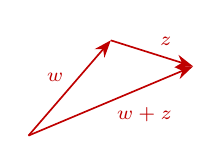
\begin{tikzpicture}[scale=.55]
  \draw[vec,red!75!black] (0,0)--node[above left=-2pt,font=\scriptsize]{$w$}
    (1.9,2.2);
  \draw[vec,red!75!black] (1.9,2.2)--node[above right=-1pt,font=\scriptsize]{$z$}
    (3.8,1.6);
  \draw[vec,red!75!black] (0,0)--node[below right=-2pt,font=\scriptsize]{$w+z$}
    (3.8,1.6);
\end{tikzpicture}}{Geometric interpretation of triangle inequality: The length
of each side of a triangle is less than or equal to the sum of the lengths of
the two other sides.}%

\subsection{Zeros of Polynomials}

Recall that a function $p\colon\F\to\F$ is called a polynomial of degree $m$
if there exist $a_0,\dots,a_m\in\F$ with $a_m\ne0$ such that
\[ p(z) = a_0+a_1z+\cdots+a_mz^m \]
for all $z\in\F$. A polynomial could have more than one degree if the
representation of $p$ in the form above were not unique. Our first task is to
show that this cannot happen.

The solutions to the equation $p(z)=0$ play a crucial role in the study of a
polynomial $p\in\Poly(\F)$. Thus these solutions have a special name.

\begin{definition}[Zero of a polynomial]\label{ax:4.5}
A number $\lambda\in\F$ is called a \emph{zero} (or \emph{root}) of a
polynomial $p\in\Poly(\F)$ if
\[ p(\lambda)=0. \]
\end{definition}

The next result is the key tool that we will use to show that the degree of a
polynomial is unique.

\begin{result}[Each zero of a polynomial corresponds to a degree-one
factor]\label{ax:4.6}
Suppose $m$ is a positive integer and $p\in\Poly(\F)$ is a polynomial of degree
$m$. Suppose $\lambda\in\F$. Then $p(\lambda)=0$ if and only if there exists a
polynomial $q\in\Poly(\F)$ of degree $m-1$ such that
\[ p(z) = (z-\lambda)q(z) \]
for every $z\in\F$.
\end{result}

\begin{proof}
First suppose $p(\lambda)=0$. Let $a_0,a_1,\dots,a_m\in\F$ be such that
\[ p(z) = a_0+a_1z+\cdots+a_mz^m \]
for all $z\in\F$. Then\refstepcounter{theorem}
\begin{equation*}
p(z) = p(z)-p(\lambda) = a_1(z-\lambda)+\cdots+a_m(z^m-\lambda^m)
\tag*{\thetheorem}\label{ax:4.7}
\end{equation*}
for all $z\in\F$. For each $k\in\{1,\dots,m\}$, the equation
\[ z^k-\lambda^k = (z-\lambda)\sum_{j=1}^{k}\lambda^{j-1}z^{k-j} \]
shows that $z^k-\lambda^k$ equals $z-\lambda$ times some polynomial of degree
$k-1$. Thus \ref{ax:4.7} shows that $p$ equals $z-\lambda$ times some
polynomial of degree $m-1$, as desired.

To prove the implication in the other direction, now suppose that there is a
polynomial $q\in\Poly(\F)$ such that $p(z)=(z-\lambda)q(z)$ for every
$z\in\F$. Then $p(\lambda)=(\lambda-\lambda)q(\lambda)=0$, as desired.
\end{proof}

Now we can prove that polynomials do not have too many zeros.

\begin{result}[Degree $m$ implies at most $m$ zeros]\label{ax:4.8}
Suppose $m$ is a positive integer and $p\in\Poly(\F)$ is a polynomial of degree
$m$. Then $p$ has at most $m$ zeros in $\F$.
\end{result}

\begin{proof}
We will use induction on $m$. The desired result holds if $m=1$ because if
$a_1\ne0$ then the polynomial $a_0+a_1z$ has only one zero (which equals
$-a_0/a_1$). Thus assume that $m>1$ and the desired result holds for $m-1$.

If $p$ has no zeros in $\F$, then the desired result holds and we are done.
Thus suppose $p$ has a zero $\lambda\in\F$. By \ref{ax:4.6}, there is
polynomial $q\in\Poly(\F)$ of degree $m-1$ such that
\[ p(z) = (z-\lambda)q(z) \]
for every $z\in\F$. Our induction hypothesis implies that $q$ has at most $m-1$
zeros in $\F$. The equation above shows that the zeros of $p$ in $\F$ are
exactly the zeros of $q$ in $\F$ along with $\lambda$. Thus $p$ has at most $m$
zeros in $\F$.
\end{proof}

The result above implies that the coefficients of a polynomial are uniquely
determined (because if a polynomial had two different sets of coefficients,
then subtracting the two representations of the polynomial would give a
polynomial with some nonzero coefficients but infinitely many zeros). In
particular, the degree of a polynomial is uniquely defined.

\marginnote{The $0$ polynomial is declared to have degree $-\infty$ so that
exceptions are not needed for various reasonable results such as
$\deg(pq)=\deg p+\deg q$.}%
Recall that the degree of the $0$ polynomial is defined to be $-\infty$. When
necessary, use the expected arithmetic with $-\infty$. For example,
$-\infty<m$ and $-\infty+m=-\infty$ for every integer $m$.

\subsection{Division Algorithm for Polynomials}

If $p$ and $s$ are nonnegative integers, with $s\ne0$, then there exist
nonnegative integers $q$ and $r$ such that
\[ p = sq+r \]
and $r<s$. Think of dividing $p$ by $s$, getting quotient $q$ with remainder
$r$. Our next result gives an analogous result for polynomials. Thus the next
result is often called the division algorithm for polynomials, although as
stated here it is not really an algorithm, just a useful result.

\marginnote{Think of the division algorithm for polynomials as giving a
remainder polynomial $r$ when the polynomial $p$ is divided by the polynomial
$s$.}%
The division algorithm for polynomials could be proved without using any linear
algebra. However, as is appropriate for a linear algebra textbook, the proof
given here uses linear algebra techniques and makes nice use of a basis of
$\Poly_n(\F)$, which is the $(n+1)$-dimensional vector space of polynomials
with coefficients in $\F$ and of degree at most $n$.

\begin{result}[Division algorithm for polynomials]\label{ax:4.9}
Suppose that $p,s\in\Poly(\F)$, with $s\ne0$. Then there exist unique
polynomials $q,r\in\Poly(\F)$ such that
\[ p = sq+r \]
and $\deg r<\deg s$.
\end{result}

\begin{proof}
Let $n=\deg p$ and let $m=\deg s$. If $n<m$, then take $q=0$ and $r=p$ to get
the desired equation $p=sq+r$ with $\deg r<\deg s$. Thus we now assume that
$n\ge m$.

The list\refstepcounter{theorem}
\begin{equation*}
1,z,\dots,z^{m-1},s,zs,\dots,z^{n-m}s
\tag*{\thetheorem}\label{ax:4.10}
\end{equation*}
is linearly independent in $\Poly_n(\F)$ because each polynomial in this list
has a different degree. Also, the list \ref{ax:4.10} has length $n+1$, which
equals $\dim\Poly_n(\F)$. Hence \ref{ax:4.10} is a basis of $\Poly_n(\F)$
[by \ref{ax:2.38}].

Because $p\in\Poly_n(\F)$ and \ref{ax:4.10} is a basis of $\Poly_n(\F)$, there
exist unique constants $a_0,a_1,\dots,a_{m-1}\in\F$ and
$b_0,b_1,\dots,b_{n-m}\in\F$ such that\refstepcounter{theorem}
\begin{align*}
p &= a_0+a_1z+\cdots+a_{m-1}z^{m-1}+b_0s+b_1zs+\cdots+b_{n-m}z^{n-m}s
  \tag*{\thetheorem}\label{ax:4.11}\\
  &= \underbrace{a_0+a_1z+\cdots+a_{m-1}z^{m-1}}_{r}
     +s(\underbrace{b_0+b_1z+\cdots+b_{n-m}z^{n-m}}_{q}).
\end{align*}
With $r$ and $q$ as defined above, we see that $p$ can be written as
$p=sq+r$ with $\deg r<\deg s$, as desired.

The uniqueness of $q,r\in\Poly(\F)$ satisfying these conditions follows from
the uniqueness of the constants $a_0,a_1,\dots,a_{m-1}\in\F$ and
$b_0,b_1,\dots,b_{n-m}\in\F$ satisfying \ref{ax:4.11}.
\end{proof}

\subsection{\texorpdfstring{Factorization of Polynomials over $\C$}%
{Factorization of Polynomials over C}}

\marginnote[-4em]{The fundamental theorem of algebra is an existence theorem. Its
proof does not lead to a method for finding zeros. The quadratic formula gives
the zeros explicitly for polynomials of degree $2$. Similar but more
complicated formulas exist for polynomials of degree $3$ and $4$. No such
formulas exist for polynomials of degree $5$ and above.}%
We have been handling polynomials with complex coefficients and polynomials
with real coefficients simultaneously, letting $\F$ denote $\R$ or $\C$. Now we
will see differences between these two cases. First we treat polynomials with
complex coefficients. Then we will use those results to prove corresponding
results for polynomials with real coefficients.

Our proof of the fundamental theorem of algebra implicitly uses the result that
a continuous real-valued function on a closed disk in $\R^2$ attains a minimum
value. A web search can lead you to several other proofs of the fundamental
theorem of algebra. The proof using Liouville's theorem is particularly nice if
you are comfortable with analytic functions. All proofs of the fundamental
theorem of algebra need to use some analysis, because the result is not true if
$\C$ is replaced, for example, with the set of numbers of the form $c+di$ where
$c,d$ are rational numbers.

\begin{result}[Fundamental theorem of algebra, first version]\label{ax:4.12}
Every nonconstant polynomial with complex coefficients has a zero in $\C$.
\end{result}

\begin{proof}
De Moivre's theorem, which you can prove using induction on $k$ and the
addition formulas for cosine and sine, states that if $k$ is a positive integer
and $\theta\in\R$, then
\[ (\cos\theta+i\sin\theta)^k = \cos k\theta+i\sin k\theta. \]

Suppose $w\in\C$ and $k$ is a positive integer. Using polar coordinates, we
know that there exist $r\ge0$ and $\theta\in\R$ such that
\[ r(\cos\theta+i\sin\theta) = w. \]
De Moivre's theorem implies that
\[ \Bigl(r^{1/k}(\cos\tfrac{\theta}{k}+i\sin\tfrac{\theta}{k})
   \Bigr)^{k} = w. \]
Thus every complex number has a $k^{\text{th}}$ root, a fact that we will soon
use.

Suppose $p$ is a nonconstant polynomial with complex coefficients and
highest-order nonzero term $c_mz^m$. Then $\abs{p(z)}\to\infty$ as
$\abs{z}\to\infty$ (because $\abs{p(z)}/\abs{z^m}\to\abs{c_m}$ as
$\abs{z}\to\infty$). Thus the continuous function $z\mapsto\abs{p(z)}$ has a
global minimum at some point $\zeta\in\C$. To show that $p(\zeta)=0$, suppose
that $p(\zeta)\ne0$.

Define a new polynomial $q$ by
\[ q(z) = \frac{p(z+\zeta)}{p(\zeta)}. \]
The function $z\mapsto\abs{q(z)}$ has a global minimum value of $1$ at $z=0$.
Write
\[ q(z) = 1+a_kz^k+\cdots+a_mz^m, \]
where $k$ is the smallest positive integer such that the coefficient of $z^k$
is nonzero; in other words, $a_k\ne0$.

Let $\beta\in\C$ be such that $\beta^k=-1/a_k$. There is a constant
$c>1$ such that if $t\in(0,1)$, then
\begin{align*}
\abs{q(t\beta)} &\le \abs{1+a_kt^k\beta^k}+t^{k+1}c\\
  &= 1-t^k(1-tc).
\end{align*}
Thus taking $t$ to be $1/(2c)$ in the inequality above, we have
$\abs{q(t\beta)}<1$, which contradicts the assumption that the global minimum
of $z\mapsto\abs{q(z)}$ is $1$. This contradiction implies that $p(\zeta)=0$,
showing that $p$ has a zero, as desired.
\end{proof}

Computers can use clever numerical methods to find good approximations to the
zeros of any polynomial, even when exact zeros cannot be found. For example, no
one will ever give an exact formula for a zero of the polynomial $p$ defined by
\[ p(x) = x^5-5x^4-6x^3+17x^2+4x-7. \]
However, a computer can find that the zeros of $p$ are approximately the five
numbers $-1.87$, $-0.74$, $0.62$, $1.47$, $5.51$.

The first version of the fundamental theorem of algebra leads to the following
factorization result for polynomials with complex coefficients. Note that in
this factorization, the zeros of $p$ are the numbers $\lambda_1,\dots,\lambda_m$,
which are the only values of $z$ for which the right side of the equation in the
next result equals $0$.

\begin{result}[Fundamental theorem of algebra, second version]\label{ax:4.13}
If $p\in\Poly(\C)$ is a nonconstant polynomial, then $p$ has a unique
factorization (except for the order of the factors) of the form
\[ p(z) = c(z-\lambda_1)\cdots(z-\lambda_m), \]
where $c,\lambda_1,\dots,\lambda_m\in\C$.
\end{result}

\begin{proof}
Let $p\in\Poly(\C)$ and let $m=\deg p$. We will use induction on $m$. If
$m=1$, then the desired factorization exists and is unique. So assume that
$m>1$ and that the desired factorization exists and is unique for all
polynomials of degree $m-1$.

First we will show that the desired factorization of $p$ exists. By the first
version of the fundamental theorem of algebra (\ref{ax:4.12}), $p$ has a zero
$\lambda\in\C$. By \ref{ax:4.6}, there is a polynomial $q$ of degree $m-1$ such
that
\[ p(z) = (z-\lambda)q(z) \]
for all $z\in\C$. Our induction hypothesis implies that $q$ has the desired
factorization, which when plugged into the equation above gives the desired
factorization of $p$.

Now we turn to the question of uniqueness. The number $c$ is uniquely
determined as the coefficient of $z^m$ in $p$. So we only need to show that
except for the order, there is only one way to choose
$\lambda_1,\dots,\lambda_m$. If
\[ (z-\lambda_1)\cdots(z-\lambda_m) = (z-\tau_1)\cdots(z-\tau_m) \]
for all $z\in\C$, then because the left side of the equation above equals $0$
when $z=\lambda_1$, one of the $\tau$'s on the right side equals $\lambda_1$.
Relabeling, we can assume that $\tau_1=\lambda_1$. Now if $z\ne\lambda_1$, we
can divide both sides of the equation above by $z-\lambda_1$, getting
\[ (z-\lambda_2)\cdots(z-\lambda_m) = (z-\tau_2)\cdots(z-\tau_m) \]
for all $z\in\C$ except possibly $z=\lambda_1$. Actually the equation above
holds for all $z\in\C$, because otherwise by subtracting the right side from
the left side we would get a nonzero polynomial that has infinitely many zeros.
The equation above and our induction hypothesis imply that except for the
order, the $\lambda$'s are the same as the $\tau$'s, completing the proof of
uniqueness.
\end{proof}

\subsection{\texorpdfstring{Factorization of Polynomials over $\R$}%
{Factorization of Polynomials over R}}

\marginnote{The failure of the fundamental theorem of algebra for $\R$ accounts
for the differences between linear algebra on real and complex vector spaces,
as we will see in later chapters.}%
A polynomial with real coefficients may have no real zeros. For example, the
polynomial $1+x^2$ has no real zeros.

To obtain a factorization theorem over $\R$, we will use our factorization
theorem over $\C$. We begin with the next result.

\begin{result}[Polynomials with real coefficients have nonreal zeros in
pairs]\label{ax:4.14}
Suppose $p\in\Poly(\C)$ is a polynomial with real coefficients. If
$\lambda\in\C$ is a zero of $p$, then so is $\overline{\lambda}$.
\end{result}

\begin{proof}
Let
\[ p(z) = a_0+a_1z+\cdots+a_mz^m, \]
where $a_0,\dots,a_m$ are real numbers. Suppose $\lambda\in\C$ is a zero of
$p$. Then
\[ a_0+a_1\lambda+\cdots+a_m\lambda^m = 0. \]
Take the complex conjugate of both sides of this equation, obtaining
\[ a_0+a_1\overline{\lambda}+\cdots+a_m\overline{\lambda}^m = 0, \]
where we have used basic properties of the complex conjugate (see
\ref{ax:4.4}). The equation above shows that $\overline{\lambda}$ is a zero of
$p$.
\end{proof}

\marginnote{Think about the quadratic formula in connection with the result
below.}%
We want a factorization theorem for polynomials with real coefficients. We
begin with the following result.

\begin{result}[Factorization of a quadratic polynomial]\label{ax:4.15}
Suppose $b,c\in\R$. Then there is a polynomial factorization of the form
\[ x^2+bx+c = (x-\lambda_1)(x-\lambda_2) \]
with $\lambda_1,\lambda_2\in\R$ if and only if $b^2\ge4c$.
\end{result}

\begin{proof}
Notice that
\[ x^2+bx+c = \Bigl(x+\frac{b}{2}\Bigr)^2+\Bigl(c-\frac{b^2}{4}\Bigr). \]

\marginnote{The equation above is the basis of the technique called completing
the square.}%
First suppose $b^2<4c$. Then the right side of the equation above is positive
for every $x\in\R$. Hence the polynomial $x^2+bx+c$ has no real zeros and thus
cannot be factored in the form $(x-\lambda_1)(x-\lambda_2)$ with
$\lambda_1,\lambda_2\in\R$.

Conversely, now suppose $b^2\ge4c$. Then there is a real number $d$ such that
$d^2=b^2/4-c$. From the displayed equation above, we have
\begin{align*}
x^2+bx+c &= \Bigl(x+\frac{b}{2}\Bigr)^2-d^2\\
  &= \Bigl(x+\frac{b}{2}+d\Bigr)\Bigl(x+\frac{b}{2}-d\Bigr),
\end{align*}
which gives the desired factorization.
\end{proof}

The next result gives a factorization of a polynomial over $\R$. The idea of
the proof is to use the second version of the fundamental theorem of algebra
(\ref{ax:4.13}), which gives a factorization of $p$ as a polynomial with
complex coefficients. Complex but nonreal zeros of $p$ come in pairs; see
\ref{ax:4.14}. Thus if the factorization of $p$ as an element of $\Poly(\C)$
includes terms of the form $(x-\lambda)$ with $\lambda$ a nonreal complex
number, then $(x-\overline{\lambda})$ is also a term in the factorization.
Multiplying together these two terms, we get
\[ x^2-2(\Re\lambda)x+\abs{\lambda}^2, \]
which is a quadratic term of the required form.

The idea sketched in the paragraph above almost provides a proof of the
existence of our desired factorization. However, we need to be careful about
one point. Suppose $\lambda$ is a nonreal complex number and $(x-\lambda)$ is a
term in the factorization of $p$ as an element of $\Poly(\C)$. We are
guaranteed by \ref{ax:4.14} that $(x-\overline{\lambda})$ also appears as a
term in the factorization, but \ref{ax:4.14} does not state that these two
factors appear the same number of times, as needed to make the idea above work.
However, the proof works around this point.

In the next result, either $m$ or $M$ may equal $0$. The numbers
$\lambda_1,\dots,\lambda_m$ are precisely the real zeros of $p$, for these are
the only real values of $x$ for which the right side of the equation in the
next result equals $0$.

\begin{result}[Factorization of a polynomial over $\R$]\label{ax:4.16}
Suppose $p\in\Poly(\R)$ is a nonconstant polynomial. Then $p$ has a unique
factorization (except for the order of the factors) of the form
\[ p(x) = c(x-\lambda_1)\cdots(x-\lambda_m)(x^2+b_1x+c_1)\cdots(x^2+b_Mx+c_M), \]
where $c,\lambda_1,\dots,\lambda_m,b_1,\dots,b_M,c_1,\dots,c_M\in\R$, with
$b_k^2<4c_k$ for each $k$.
\end{result}

\begin{proof}
First we will prove that the desired factorization exists, and after that we
will prove the uniqueness.

Think of $p$ as an element of $\Poly(\C)$. If all (complex) zeros of $p$ are
real, then we have the desired factorization by \ref{ax:4.13}. Thus suppose
$p$ has a zero $\lambda\in\C$ with $\lambda\notin\R$. By \ref{ax:4.14},
$\overline{\lambda}$ is a zero of $p$. Thus we can write
\begin{align*}
p(x) &= (x-\lambda)(x-\overline{\lambda})q(x)\\
     &= \bigl(x^2-2(\Re\lambda)x+\abs{\lambda}^2\bigr)q(x)
\end{align*}
for some polynomial $q\in\Poly(\C)$ of degree two less than the degree of $p$.
If we can prove that $q$ has real coefficients, then using induction on the
degree of $p$ completes the proof of the existence part of this result.

To prove that $q$ has real coefficients, we solve the equation above for $q$,
getting
\[ q(x) = \frac{p(x)}{x^2-2(\Re\lambda)x+\abs{\lambda}^2} \]
for all $x\in\R$. The equation above implies that $q(x)\in\R$ for all
$x\in\R$. Writing
\[ q(x) = a_0+a_1x+\cdots+a_{n-2}x^{n-2}, \]
where $n=\deg p$ and $a_0,\dots,a_{n-2}\in\C$, we thus have
\[ 0 = \Im q(x) = (\Im a_0)+(\Im a_1)x+\cdots+(\Im a_{n-2})x^{n-2} \]
for all $x\in\R$. This implies that $\Im a_0,\dots,\Im a_{n-2}$ all equal $0$
(by \ref{ax:4.8}). Thus all coefficients of $q$ are real, as desired. Hence the
desired factorization exists.

Now we turn to the question of uniqueness of our factorization. A factor of $p$
of the form $x^2+b_kx+c_k$ with $b_k^2<4c_k$ can be uniquely written as
$(x-\lambda_k)(x-\overline{\lambda_k})$ with $\lambda_k\in\C$. A moment's
thought shows that two different factorizations of $p$ as an element of
$\Poly(\R)$ would lead to two different factorizations of $p$ as an element of
$\Poly(\C)$, contradicting \ref{ax:4.13}.
\end{proof}

% ------------------------------------------------------------------ exercises
\exercisesheading{4}

\begin{exercise}
Suppose $w,z\in\C$. Verify the following equalities and inequalities.
\begin{parts}
\item $z+\overline{z}=2\Re z$
\item $z-\overline{z}=2(\Im z)i$
\item $z\overline{z}=\abs{z}^2$
\item $\overline{w+z}=\overline{w}+\overline{z}$ and
  $\overline{wz}=\overline{w}\,\overline{z}$
\item $\overline{\overline{z}}=z$
\item $\abs{\Re z}\le\abs{z}$ and $\abs{\Im z}\le\abs{z}$
\item $\abs{\overline{z}}=\abs{z}$
\item $\abs{wz}=\abs{w}\,\abs{z}$
\end{parts}
\exnote{The results above are the parts of \ref{ax:4.4} that were left to the
reader.}
\end{exercise}
\begin{solution}
In this problem, let $z=a+bi$ and $w=c+di$ with $a,b,c,d\in\R$. Then
\begin{parts}
\item $z+\bar{z}=(a+bi)+(a-bi)=2a=2\mathfrak{R}z$.
\item $z-\bar{z}=(a+bi)-(a-bi)=2bi=2(\mathfrak{I}z)i$.
\item $z\bar{z}=(a+bi)(a-bi)=a^2+b^2=\abs{z}^2$.
\item $\overline{w+z}=\overline{(c+di)+(a+bi)}=\overline{(a+c)+(b+d)i}
  =(a+c)-(b+d)i=(a-bi)+(c-di)=\overline{w}+\bar{z}$ and
  $\overline{wz}=\overline{(c+di)(a+bi)}=\overline{(ac-bd)+(ad+bc)i}
  =(ac-bd)-(ad+bc)i=(c-di)(a-bi)=\overline{w}\bar{z}$.
\item $\bar{\bar{z}}=\overline{a-bi}=a+bi=z$.
\item $\abs{\mathfrak{R}z}=\abs{a}\le\sqrt{a^2+b^2}=\abs{z}$ and
  $\abs{\mathfrak{I}z}=\abs{b}\le\sqrt{a^2+b^2}=\abs{z}$.
\item $\abs{\bar{z}}=\abs{a-bi}=\sqrt{a^2+b^2}=\abs{z}$.
\item $\abs{wz}=\abs{(c+di)(a+bi)}=\abs{(ac-bd)+(ad+bc)i}
  =\sqrt{(ac-bd)^2+(ad+bc)^2}=\sqrt{(a^2+b^2)(c^2+d^2)}
  =\abs{a+bi}\abs{c+di}=\abs{z}\abs{w}$. \qedhere
\end{parts}
\end{solution}

\begin{exercise}
Prove that if $w,z\in\C$, then $\bigl\lvert\abs{w}-\abs{z}\bigr\rvert
\le\abs{w-z}$.
\exnote{The inequality above is called the \textbf{reverse triangle
inequality}.}
\end{exercise}
\begin{solution}
Let $w,z\in\C$. By the triangle inequality, we have
\[ \abs{w}=\abs{(w-z)+z}\le\abs{w-z}+\abs{z}. \]
Rearranging gives $\abs{w}-\abs{z}\le\abs{w-z}$. Similarly,
\[ \abs{z}=\abs{(z-w)+w}\le\abs{z-w}+\abs{w}=\abs{w-z}+\abs{w}, \]
which gives $\abs{z}-\abs{w}\le\abs{w-z}$, or equivalently
$-\abs{w-z}\le\abs{w}-\abs{z}$. Combining these inequalities, we get
\[ \bigl\lvert\abs{w}-\abs{z}\bigr\rvert\le\abs{w-z}. \qedhere \]
\end{solution}

\begin{exercise}
Suppose $V$ is a complex vector space and $\varphi\in V'$. Define
$\sigma\colon V\to\R$ by $\sigma(v)=\Re\varphi(v)$ for each $v\in V$. Show that
\[ \varphi(v) = \sigma(v)-i\sigma(iv) \]
for all $v\in V$.
\end{exercise}
\begin{solution}
Let $v\in V$. Then there exist $s,t\in\R$ such that
\[ \varphi(v)=s+ti. \]
Then
\[ \sigma(v)=\mathfrak{R}\varphi(v)=s \quad\text{and}\quad
   \sigma(iv)=\mathfrak{R}\varphi(iv)=\mathfrak{R}\bigl(i(s+ti)\bigr)
   =\mathfrak{R}(-t+si)=-t. \]
Therefore,
\[ \sigma(v)-i\sigma(iv)=s-i(-t)=s+ti=\varphi(v). \qedhere \]
\end{solution}

\begin{exercise}
Suppose $m$ is a positive integer. Is the set
\[ \{0\}\cup\{p\in\Poly(\F) : \deg p=m\} \]
a subspace of $\Poly(\F)$?
\end{exercise}
\begin{solution}
No, the set is not a subspace of $\Poly(\F)$. To see this, consider two
polynomials $p,q\in\Poly(\F)$ with $p(x)=x^m$ and $q(x)=-x^m+x^{m-1}$. Then
$p+q=x^{m-1}$, which has degree $m-1$ and is not in the set. Therefore, the set
is not closed under addition and hence not a subspace.
\end{solution}

\begin{exercise}
Is the set
\[ \{0\}\cup\{p\in\Poly(\F) : \deg p \text{ is even}\} \]
a subspace of $\Poly(\F)$?
\end{exercise}
\begin{solution}
No, the set is not a subspace of $\Poly(\F)$. To see this, consider two
polynomials $p,q\in\Poly(\F)$ with $p(x)=x^2$ and $q(x)=x-x^2$. Then $p+q=x$,
which has degree $1$ and is not even. Therefore, the set is not closed under
addition and hence not a subspace.
\end{solution}

\begin{exercise}
Suppose that $m$ and $n$ are positive integers with $m\le n$, and suppose
$\lambda_1,\dots,\lambda_m\in\F$. Prove that there exists a polynomial
$p\in\Poly(\F)$ with $\deg p=n$ such that
$0=p(\lambda_1)=\cdots=p(\lambda_m)$ and such that $p$ has no other zeros.
\end{exercise}
\begin{solution}
Consider the polynomial
\[ p(x)=(x-\lambda_1)^{n-m+1}(x-\lambda_2)\cdots(x-\lambda_m). \]
This polynomial has degree $n$, vanishes at $\lambda_1,\dots,\lambda_m$, and
has no other zeros. Therefore, it satisfies the required conditions.
\end{solution}

\begin{exercise}
Suppose that $m$ is a nonnegative integer, $z_1,\dots,z_{m+1}$ are distinct
elements of $\F$, and $w_1,\dots,w_{m+1}\in\F$. Prove that there exists a
unique polynomial $p\in\Poly_m(\F)$ such that
\[ p(z_k)=w_k \]
for each $k=1,\dots,m+1$.
\exnote{This result can be proved without using linear algebra. However, try to
find the clearer, shorter proof that uses some linear algebra.}
\end{exercise}
\begin{solution}
Consider the linear map $T\colon\Poly_m(\F)\to\F^{m+1}$ defined by
\[ T(p)=\bigl(p(z_1),\dots,p(z_{m+1})\bigr). \]
Since $\dim\Poly_m(\F)=m+1$ and $\dim\F^{m+1}=m+1$, it suffices to show that
$T$ is injective to conclude that it is also surjective. Suppose $T(p)=0$,
i.e., $p(z_k)=0$ for all $k=1,\dots,m+1$. Since $p$ has degree at most $m$ and
has $m+1$ distinct zeros, it must be the zero polynomial. Therefore, $T$ is
injective, and hence bijective. This shows that for any
$(w_1,\dots,w_{m+1})\in\F^{m+1}$, there exists a unique $p\in\Poly_m(\F)$ such
that $T(p)=(w_1,\dots,w_{m+1})$, which is exactly the desired polynomial.
\end{solution}

\begin{exercise}
Suppose $p\in\Poly(\C)$ has degree $m$. Prove that $p$ has $m$ distinct zeros
if and only if $p$ and its derivative $p'$ have no zeros in common.
\end{exercise}
\begin{solution}
Suppose $p$ has $m$ distinct zeros, say $z_1,\dots,z_m$. If $p$ and $p'$ have
a common zero $z_k$, then $z_k$ would be a multiple zero of $p$, contradicting
the assumption that all zeros are distinct. Hence, $p$ and $p'$ have no zeros
in common.

Conversely, suppose $p$ and $p'$ have no zeros in common. If $p$ had a
multiple zero $z$, then $p(z)=0$ and $p'(z)=0$, which would contradict the
assumption. Therefore, all zeros of $p$ are distinct.
\end{solution}

\begin{exercise}
Prove that every polynomial of odd degree with real coefficients has a real
zero.
\end{exercise}
\begin{solution}
\solnote{Appendix}{See the alternate proof at the end of this solution, which
uses the intermediate value theorem.}
Let $p(x)$ be a polynomial of odd degree with real coefficients. Since complex
zeros come in pairs, there are an even number of complex zeros. Therefore,
there must be at least one real zero.

\emph{Alternate proof.} Let $p(x)$ be a polynomial of odd degree with real
coefficients. As $x\to\infty$, $p(x)\to\infty$ or $p(x)\to-\infty$ depending
on the leading coefficient. Similarly, as $x\to-\infty$, $p(x)\to-\infty$ or
$p(x)\to\infty$. By the intermediate value theorem, since $p(x)$ is continuous
and takes on both positive and negative values, there must exist some
$x\in\R$ such that $p(x)=0$. Therefore, $p$ has a real zero.
\end{solution}

\begin{exercise}
For $p\in\Poly(\R)$, define $Tp\colon\R\to\R$ by
\[ (Tp)(x) = \begin{cases}
  \dfrac{p(x)-p(3)}{x-3} & \text{if } x\ne3,\\[2ex]
  p'(3) & \text{if } x=3
\end{cases} \]
for each $x\in\R$. Show that $Tp\in\Poly(\R)$ for every polynomial
$p\in\Poly(\R)$ and also show that $T\colon\Poly(\R)\to\Poly(\R)$ is a linear
map.
\end{exercise}
\begin{solution}
Let $p\in\Poly(\R)$. Since $p(x)-p(3)$ has a zero at $x=3$, we can factor it
as $(x-3)q(x)$ for some polynomial $q\in\Poly(\R)$. Then for $x\ne3$,
\[ (Tp)(x)=\frac{p(x)-p(3)}{x-3}=q(x), \]
and differentiating $p$ gives $p'(3)=q(3)$. Since $Tp(3)=p'(3)=q(3)$, we have
$Tp(x)=q(x)$ for all $x\in\R$. Therefore, $Tp\in\Poly(\R)$.

Let $p_1,p_2\in\Poly(\R)$ and $\alpha,\beta\in\R$. Let
$p_1(x)-p_1(3)=(x-3)q_1(x)$ and $p_2(x)-p_2(3)=(x-3)q_2(x)$ for some
$q_1,q_2\in\Poly(\R)$. Then
\[ (\alpha p_1+\beta p_2)(x)=\bigl(\alpha p_1(3)+\beta p_2(3)\bigr)
   +(x-3)\bigl(\alpha q_1(x)+\beta q_2(x)\bigr). \]
Hence, $T(\alpha p_1+\beta p_2)(x)=\alpha q_1(x)+\beta q_2(x)
=\alpha Tp_1(x)+\beta Tp_2(x)$ for all $x\in\R$. Therefore, $T$ is a linear
map.
\end{solution}

\begin{exercise}
Suppose $p\in\Poly(\C)$. Define $q\colon\C\to\C$ by
\[ q(z) = p(z)\,\overline{p(\overline{z})}. \]
Prove that $q$ is a polynomial with real coefficients.
\end{exercise}
\begin{solution}
\solnote{Appendix}{See the alternate proof at the end of this solution, which
looks at the roots of $p$.}
Let $p\in\Poly(\C)$ have the form $p(z)=a_0+a_1z+\cdots+a_nz^n$ with
$a_k\in\C$. Then
\[ \overline{p(\bar{z})}=\overline{\sum_{i=0}^{n}a_i\bar{z}^i}
   =\sum_{i=0}^{n}\bar{a}_iz^i. \]
Therefore,
\[ q(z)=p(z)\overline{p(\bar{z})}
   =\biggl(\sum_{i=0}^{n}a_iz^i\biggr)\biggl(\sum_{j=0}^{n}\bar{a}_jz^j\biggr)
   =\sum_{k=0}^{2n}\biggl(\sum_{i+j=k}a_i\bar{a}_j\biggr)z^k. \]
Let $b_m$ denote the coefficient of $z^m$ in $q(z)$. Then
\[ b_m=\sum_{i+j=m}a_i\bar{a}_j=\sum_{i+j=m}\bar{a}_ja_i=\overline{b_m}. \]
Hence, $b_m\in\R$ for each $m=0,1,\dots,2n$. Therefore, $q$ is a polynomial
with real coefficients.

\emph{Alternate proof.} If $p=0$, then $q=0$ is a polynomial with real
coefficients. Otherwise, let $n=\deg p$. Then we may write
\[ p(z)=\alpha(z-\lambda_1)(z-\lambda_2)\cdots(z-\lambda_n), \]
where $\alpha\in\C$ and $\lambda_1,\lambda_2,\dots,\lambda_n\in\C$ are the
roots of $p$. Then
\begin{align*}
q(z)=p(z)\overline{p(\bar{z})}
  &=\alpha(z-\lambda_1)(z-\lambda_2)\cdots(z-\lambda_n)\\
  &\quad\cdot\bar{\alpha}(z-\overline{\lambda_1})(z-\overline{\lambda_2})
    \cdots(z-\overline{\lambda_n}).
\end{align*}
Note that the product contains the term $\alpha\bar{\alpha}=\abs{\alpha}^2\in\R$,
as well as the pairs
\[ (z-\lambda_i)(z-\overline{\lambda_i})=z^2-2\mathfrak{R}(\lambda_i)z
   +\abs{\lambda_i}^2. \]
Each such pair contributes a quadratic polynomial with real coefficients. Since
the product of polynomials with real coefficients also has real coefficients,
it follows that $q(z)$ is a polynomial with real coefficients.
\end{solution}

\begin{exercise}
Suppose $m$ is a nonnegative integer and $p\in\Poly_m(\C)$ is such that there
are distinct real numbers $x_0,x_1,\dots,x_m$ with $p(x_k)\in\R$ for each
$k=0,1,\dots,m$. Prove that all coefficients of $p$ are real.
\end{exercise}
\begin{solution}
Let $p(x_k)=y_k\in\R$ for each $k=0,1,\dots,m$. By Exercise~4.7 with $\F=\R$,
there exists a polynomial $q\in\Poly_m(\R)$ that satisfies $q(x_k)=y_k$ for
each $k=0,1,\dots,m$. Note that this polynomial must be the same as the
original $p\in\Poly_m(\C)$ because a polynomial of degree at most $m$ is
uniquely determined by its values at $m+1$ distinct points. Therefore, all
coefficients of $p$ are real.
\end{solution}

\begin{exercise}
Suppose $p\in\Poly(\F)$ with $p\ne0$. Let $U=\{pq : q\in\Poly(\F)\}$.
\begin{parts}
\item Show that $\dim\Poly(\F)/U=\deg p$.
\item Find a basis of $\Poly(\F)/U$.
\end{parts}
\end{exercise}
\begin{solution}\leavevmode
\begin{parts}
\item We first show that $U$ is a subspace of $\Poly(\F)$. Clearly, $0\in U$
  since $0=p\cdot0$. If $u_1,u_2\in U$, then $u_1=pq_1$ and $u_2=pq_2$ for some
  $q_1,q_2\in\Poly(\F)$. For any scalars $\alpha,\beta\in\F$, we have
  $\alpha u_1+\beta u_2=\alpha pq_1+\beta pq_2=p(\alpha q_1+\beta q_2)\in U$.
  Therefore, $U$ is closed under addition and scalar multiplication, and hence
  $U$ is a subspace of $\Poly(\F)$.

  Now let $r\in\Poly(\F)$. By the division algorithm for polynomials, there
  exist unique polynomials $q_0\in\Poly(\F)$ and $s\in\Poly(\F)$ with
  $\deg s<\deg p$ such that $r=pq_0+s$. This shows that every polynomial in
  $\Poly(\F)$ can be written as an element of $U$ plus a polynomial of degree
  less than $\deg p$. Consider the map
  $T\colon\Poly_{\deg p-1}(\F)\to\Poly(\F)/U$ defined by $T(s)=s+U$. This map
  is linear and surjective, and $\nul T$ is trivial since if $s+U=U$, then
  $s\in U$, which implies $s=pq$ for some $q\in\Poly(\F)$. But
  $\deg s<\deg p$, so $s$ must be zero. Therefore, $T$ is an isomorphism, and
  we conclude that $\dim\Poly(\F)/U=\dim\Poly_{\deg p-1}(\F)=\deg p$.
\item A basis of $\Poly(\F)/U$ is given by the images of the standard basis of
  $\Poly_{\deg p-1}(\F)$ under $T$, namely
  $\{1+U,x+U,\dots,x^{\deg p-1}+U\}$. \qedhere
\end{parts}
\end{solution}

\begin{exercise}
Suppose $p,q\in\Poly(\C)$ are nonconstant polynomials with no zeros in common.
Let $m=\deg p$ and $n=\deg q$. Use linear algebra as outlined below in
(a)--(c) to prove that there exist $r\in\Poly_{n-1}(\C)$ and
$s\in\Poly_{m-1}(\C)$ such that
\[ rp+sq=1. \]
\begin{parts}
\item Define $T\colon\Poly_{n-1}(\C)\times\Poly_{m-1}(\C)\to\Poly_{m+n-1}(\C)$
  by
  \[ T(r,s)=rp+sq. \]
  Show that the linear map $T$ is injective.
\item Show that the linear map $T$ in (a) is surjective.
\item Use (b) to conclude that there exist $r\in\Poly_{n-1}(\C)$ and
  $s\in\Poly_{m-1}(\C)$ such that $rp+sq=1$.
\end{parts}
\end{exercise}
\begin{solution}
\solnote{Manual Remark}{In part (a), one may also observe that a multiple of
$p$ and $q$ must have $\deg p+\deg q$, but
$\deg rp=\deg r+\deg p\le n-1+m$.}
\begin{parts}
\item To show that $T$ is injective, suppose that $T(r,s)=rp+sq=0$ for some
  $(r,s)\in\Poly_{n-1}(\C)\times\Poly_{m-1}(\C)$. Then $rp=-sq$ so that $q$
  divides $rp$. Since $p$ and $q$ have no zeros in common, $q$ must divide
  $r$. But $\deg r<\deg q$, so the only possibility is that $r=0$. Then
  $-sq=0$. Since $q$ is nonconstant, this implies that $s=0$. Therefore,
  $\nul T=\{(0,0)\}$, and hence $T$ is injective.
\item To show that $T$ is surjective, note that
  $\dim\bigl(\Poly_{n-1}(\C)\times\Poly_{m-1}(\C)\bigr)=n+m
  =\dim\Poly_{m+n-1}(\C)$. Since $T$ is a linear map between vector spaces of
  the same finite dimension, and we have already shown that $T$ is injective,
  it follows that $T$ is also surjective.
\item Since $T$ is surjective, for the polynomial $1\in\Poly_{m+n-1}(\C)$,
  there exist $r\in\Poly_{n-1}(\C)$ and $s\in\Poly_{m-1}(\C)$ such that
  $T(r,s)=rp+sq=1$. \qedhere
\end{parts}
\end{solution}

\renewcommand\thesection{\thechapter\Alph{section}}


% Chapter 5: assembled from chapters/ch05/*.tex
\chapter{Eigenvalues and Eigenvectors}

Linear maps from one vector space to another vector space were the objects of
study in Chapter~3. Now we begin our investigation of operators, which are
linear maps from a vector space to itself. Their study constitutes the most
important part of linear algebra.

To learn about an operator, we might try restricting it to a smaller subspace.
Asking for that restriction to be an operator will lead us to the notion of
invariant subspaces. Each one-dimensional invariant subspace arises from a
vector that the operator maps into a scalar multiple of the vector. This path
will lead us to eigenvectors and eigenvalues.

We will then prove one of the most important results in linear algebra: every
operator on a finite-dimensional nonzero complex vector space has an
eigenvalue. This result will allow us to show that for each operator on a
finite-dimensional complex vector space, there is a basis of the vector space
with respect to which the matrix of the operator has at least almost half its
entries equal to $0$.

\begin{definition*}[Standing assumptions for this chapter]\leavevmode
\begin{itemize}
\item $\F$ denotes $\R$ or $\C$.
\item $V$ denotes a vector space over $\F$.
\end{itemize}
\end{definition*}

% Source: book pp. 133--142 (PDF 147--156); solutions pp. 135--151, 175.
\section{Invariant Subspaces}

\subsection{Eigenvalues}

\begin{definition}[Operator]\label{ax:5.1}
A linear map from a vector space to itself is called an \emph{operator}.
\end{definition}

\marginnote{Recall that we defined the notation $\Lin(V)$ to mean
$\Lin(V,V)$.}%
Suppose $T\in\Lin(V)$. If $m\ge2$ and
\[ V = V_1\oplus\cdots\oplus V_m, \]
where each $V_k$ is a nonzero subspace of $V$, then to understand the behavior
of $T$ we only need to understand the behavior of each $T|_{V_k}$; here
$T|_{V_k}$ denotes the restriction of $T$ to the smaller domain $V_k$. Dealing
with $T|_{V_k}$ should be easier than dealing with $T$ because $V_k$ is a
smaller vector space than $V$.

However, if we intend to apply tools useful in the study of operators (such as
taking powers), then we have a problem: $T|_{V_k}$ may not map $V_k$ into
itself; in other words, $T|_{V_k}$ may not be an operator on $V_k$. Thus we are
led to consider only decompositions of $V$ of the form above in which $T$ maps
each $V_k$ into itself. Hence we now give a name to subspaces of $V$ that get
mapped into themselves by $T$.

\begin{definition}[Invariant subspace]\label{ax:5.2}
Suppose $T\in\Lin(V)$. A subspace $U$ of $V$ is called \emph{invariant} under
$T$ if $Tu\in U$ for every $u\in U$.
\end{definition}

Thus $U$ is invariant under $T$ if $T|_U$ is an operator on $U$.

\begin{example}[Subspace invariant under differentiation operator]\label{ax:5.3}
Suppose that $T\in\Lin(\Poly(\R))$ is defined by $Tp=p'$. Then $\Poly_4(\R)$,
which is a subspace of $\Poly(\R)$, is invariant under $T$ because if
$p\in\Poly(\R)$ has degree at most $4$, then $p'$ also has degree at most $4$.
\end{example}

\begin{example}[Four invariant subspaces, not necessarily all different]\label{ax:5.4}
If $T\in\Lin(V)$, then the following subspaces of $V$ are all invariant under
$T$.
\begin{description}[font=\normalfont,align=right,labelwidth=3.4em,
  labelsep=.8em,leftmargin=4.2em,itemsep=1pt,topsep=3pt]
\item[$\{0\}$] The subspace $\{0\}$ is invariant under $T$ because if
  $u\in\{0\}$, then $u=0$ and hence $Tu=0\in\{0\}$.
\item[$V$] The subspace $V$ is invariant under $T$ because if $u\in V$, then
  $Tu\in V$.
\item[$\nul T$] The subspace $\nul T$ is invariant under $T$ because if
  $u\in\nul T$, then $Tu=0$, and hence $Tu\in\nul T$.
\item[$\range T$] The subspace $\range T$ is invariant under $T$ because if
  $u\in\range T$, then $Tu\in\range T$.
\end{description}
\end{example}

Must an operator $T\in\Lin(V)$ have any invariant subspaces other than $\{0\}$
and $V$? Later we will see that this question has an affirmative answer if $V$
is finite-dimensional and $\dim V>1$ (for $\F=\C$) or $\dim V>2$ (for
$\F=\R$); see \ref{ax:5.19} and Exercise~29 in Section~5B.

The previous example noted that $\nul T$ and $\range T$ are invariant under
$T$. However, these subspaces do not necessarily provide easy answers to the
question above about the existence of invariant subspaces other than $\{0\}$
and $V$, because $\nul T$ may equal $\{0\}$ and $\range T$ may equal $V$ (this
happens when $T$ is invertible).

We will return later to a deeper study of invariant subspaces. Now we turn to
an investigation of the simplest possible nontrivial invariant
subspaces---invariant subspaces of dimension one.

Take any $v\in V$ with $v\ne0$ and let $U$ equal the set of all scalar
multiples of $v$:
\[ U = \{\lambda v : \lambda\in\F\} = \spn(v). \]
Then $U$ is a one-dimensional subspace of $V$ (and every one-dimensional
subspace of $V$ is of this form for an appropriate choice of $v$). If $U$ is
invariant under an operator $T\in\Lin(V)$, then $Tv\in U$, and hence there is
a scalar $\lambda\in\F$ such that
\[ Tv = \lambda v. \]
Conversely, if $Tv=\lambda v$ for some $\lambda\in\F$, then $\spn(v)$ is a
one-dimensional subspace of $V$ invariant under $T$.

The equation $Tv=\lambda v$, which we have just seen is intimately connected
with one-dimensional invariant subspaces, is important enough that the scalars
$\lambda$ and vectors $v$ satisfying it are given special names.

\begin{definition}[Eigenvalue]\label{ax:5.5}
Suppose $T\in\Lin(V)$. A number $\lambda\in\F$ is called an \emph{eigenvalue}
of $T$ if there exists $v\in V$ such that $v\ne0$ and $Tv=\lambda v$.
\end{definition}

\marginnote{The word \textbf{eigenvalue} is half-German, half-English. The
German prefix \textbf{eigen} means ``own'' in the sense of characterizing an
intrinsic property.}%
In the definition above, we require that $v\ne0$ because every scalar
$\lambda\in\F$ satisfies $T0=\lambda0$.

The comments above show that $V$ has a one-dimensional subspace invariant under
$T$ if and only if $T$ has an eigenvalue.

\begin{example}[Eigenvalue]\label{ax:5.6}
Define an operator $T\in\Lin(\F^3)$ by
\[ T(x,y,z) = (7x+3z,\,3x+6y+9z,\,-6y) \]
for $(x,y,z)\in\F^3$. Then $T(3,1,-1)=(18,6,-6)=6(3,1,-1)$. Thus $6$ is an
eigenvalue of $T$.
\end{example}

\marginnote[-4mm]{Reminder: $I\in\Lin(V)$ is the identity operator. Thus $Iv=v$
for all $v\in V$.}%
The equivalences in the next result, along with many deep results in linear
algebra, are valid only in the context of finite-dimensional vector spaces.

\begin{result}[Equivalent conditions to be an eigenvalue]\label{ax:5.7}
Suppose $V$ is finite-dimensional, $T\in\Lin(V)$, and $\lambda\in\F$. Then the
following are equivalent.
\begin{parts}
\item $\lambda$ is an eigenvalue of $T$.
\item $T-\lambda I$ is not injective.
\item $T-\lambda I$ is not surjective.
\item $T-\lambda I$ is not invertible.
\end{parts}
\end{result}

\begin{proof}
Conditions (a) and (b) are equivalent because the equation $Tv=\lambda v$ is
equivalent to the equation $(T-\lambda I)v=0$. Conditions (b), (c), and (d) are
equivalent by \ref{ax:3.65}.
\end{proof}

\begin{definition}[Eigenvector]\label{ax:5.8}
Suppose $T\in\Lin(V)$ and $\lambda\in\F$ is an eigenvalue of $T$. A vector
$v\in V$ is called an \emph{eigenvector} of $T$ corresponding to $\lambda$ if
$v\ne0$ and $Tv=\lambda v$.
\end{definition}

In other words, a nonzero vector $v\in V$ is an eigenvector of an operator
$T\in\Lin(V)$ if and only if $Tv$ is a scalar multiple of $v$. Because
$Tv=\lambda v$ if and only if $(T-\lambda I)v=0$, a vector $v\in V$ with
$v\ne0$ is an eigenvector of $T$ corresponding to $\lambda$ if and only if
$v\in\nul(T-\lambda I)$.

\begin{example}[Eigenvalues and eigenvectors]\label{ax:5.9}
Suppose $T\in\Lin(\F^2)$ is defined by $T(w,z)=(-z,w)$.
\begin{parts}
\item First consider the case $\F=\R$. Then $T$ is a counterclockwise rotation
  by $90^\circ$ about the origin in $\R^2$. An operator has an eigenvalue if and
  only if there exists a nonzero vector in its domain that gets sent by the
  operator to a scalar multiple of itself. A $90^\circ$ counterclockwise
  rotation of a nonzero vector in $\R^2$ cannot equal a scalar multiple of
  itself. Conclusion: if $\F=\R$, then $T$ has no eigenvalues (and thus has no
  eigenvectors).
\item Now consider the case $\F=\C$. To find eigenvalues of $T$, we must find
  the scalars $\lambda$ such that $T(w,z)=\lambda(w,z)$ has some solution other
  than $w=z=0$. The equation $T(w,z)=\lambda(w,z)$ is equivalent to the
  simultaneous equations\refstepcounter{theorem}%
  \[ -z=\lambda w,\qquad w=\lambda z. \tag*{\thetheorem}\label{ax:5.10} \]
  Substituting the value for $w$ given by the second equation into the first
  equation gives
  \[ -z = \lambda^2 z. \]
  Now $z$ cannot equal $0$ [otherwise \ref{ax:5.10} implies that $w=0$; we are
  looking for solutions to \ref{ax:5.10} such that $(w,z)$ is not the $0$
  vector], so the equation above leads to the equation
  \[ -1 = \lambda^2. \]
  The solutions to this equation are $\lambda=i$ and $\lambda=-i$.

  You can verify that $i$ and $-i$ are eigenvalues of $T$. Indeed, the
  eigenvectors corresponding to the eigenvalue $i$ are the vectors of the form
  $(w,-wi)$, with $w\in\C$ and $w\ne0$. Furthermore, the eigenvectors
  corresponding to the eigenvalue $-i$ are the vectors of the form $(w,wi)$,
  with $w\in\C$ and $w\ne0$.
\end{parts}
\end{example}

In the next proof, we again use the equivalence
\[ Tv=\lambda v \iff (T-\lambda I)v=0. \]

\begin{result}[Linearly independent eigenvectors]\label{ax:5.11}
Suppose $T\in\Lin(V)$. Then every list of eigenvectors of $T$ corresponding to
distinct eigenvalues of $T$ is linearly independent.
\end{result}

\begin{proof}
Suppose the desired result is false. Then there exists a smallest positive
integer $m$ such that there exists a linearly dependent list $v_1,\dots,v_m$ of
eigenvectors of $T$ corresponding to distinct eigenvalues
$\lambda_1,\dots,\lambda_m$ of $T$ (note that $m\ge2$ because an eigenvector
is, by definition, nonzero). Thus there exist $a_1,\dots,a_m\in\F$, none of
which are $0$ (because of the minimality of $m$), such that
\[ a_1v_1+\cdots+a_mv_m = 0. \]
Apply $T-\lambda_mI$ to both sides of the equation above, getting
\[ a_1(\lambda_1-\lambda_m)v_1+\cdots+a_{m-1}(\lambda_{m-1}-\lambda_m)v_{m-1}
   = 0. \]
Because the eigenvalues $\lambda_1,\dots,\lambda_m$ are distinct, none of the
coefficients above equal $0$. Thus $v_1,\dots,v_{m-1}$ is a linearly dependent
list of $m-1$ eigenvectors of $T$ corresponding to distinct eigenvalues,
contradicting the minimality of $m$. This contradiction completes the proof.
\end{proof}

The result above leads to a short proof of the result below, which puts an
upper bound on the number of distinct eigenvalues that an operator can have.

\begin{result}[Operator cannot have more eigenvalues than dimension of vector
space]\label{ax:5.12}
Suppose $V$ is finite-dimensional. Then each operator on $V$ has at most
$\dim V$ distinct eigenvalues.
\end{result}

\begin{proof}
Let $T\in\Lin(V)$. Suppose $\lambda_1,\dots,\lambda_m$ are distinct eigenvalues
of $T$. Let $v_1,\dots,v_m$ be corresponding eigenvectors. Then \ref{ax:5.11}
implies that the list $v_1,\dots,v_m$ is linearly independent. Thus
$m\le\dim V$ (see \ref{ax:2.22}), as desired.
\end{proof}

\subsection{Polynomials Applied to Operators}

The main reason that a richer theory exists for operators (which map a vector
space into itself) than for more general linear maps is that operators can be
raised to powers. In this subsection we define that notion and the concept of
applying a polynomial to an operator. This concept will be the key tool that
we use in the next section when we prove that every operator on a nonzero
finite-dimensional complex vector space has an eigenvalue.

If $T$ is an operator, then $TT$ makes sense (see \ref{ax:3.7}) and is also an
operator on the same vector space as $T$. We usually write $T^2$ instead of
$TT$. More generally, we have the following definition of $T^m$.

\begin{notation}[$T^m$]\label{ax:5.13}
Suppose $T\in\Lin(V)$ and $m$ is a positive integer.
\begin{itemize}
\item $T^m\in\Lin(V)$ is defined by $T^m=\ftimes{T\cdots T}{m\text{ times}}$.
\item $T^0$ is defined to be the identity operator $I$ on $V$.
\item If $T$ is invertible with inverse $T^{-1}$, then $T^{-m}\in\Lin(V)$ is
  defined by
  \[ T^{-m} = (T^{-1})^m. \]
\end{itemize}
\end{notation}

You should verify that if $T$ is an operator, then
\[ T^mT^n = T^{m+n} \quad\text{and}\quad (T^m)^n = T^{mn}, \]
where $m$ and $n$ are arbitrary integers if $T$ is invertible and are
nonnegative integers if $T$ is not invertible.

Having defined powers of an operator, we can now define what it means to apply
a polynomial to an operator.

\begin{notation}[$p(T)$]\label{ax:5.14}
Suppose $T\in\Lin(V)$ and $p\in\Poly(\F)$ is a polynomial given by
\[ p(z) = a_0+a_1z+a_2z^2+\cdots+a_mz^m \]
for all $z\in\F$. Then $p(T)$ is the operator on $V$ defined by
\[ p(T) = a_0I+a_1T+a_2T^2+\cdots+a_mT^m. \]
\end{notation}

This is a new use of the symbol $p$ because we are applying $p$ to operators,
not just elements of $\F$. The idea here is that to evaluate $p(T)$, we simply
replace $z$ with $T$ in the expression defining $p$. Note that the constant
term $a_0$ in $p(z)$ becomes the operator $a_0I$ (which is a reasonable choice
because $a_0=a_0z^0$ and thus we should replace $a_0$ with $a_0T^0$, which
equals $a_0I$).

\begin{example}[A polynomial applied to the differentiation
operator]\label{ax:5.15}
Suppose $D\in\Lin(\Poly(\R))$ is the differentiation operator defined by
$Dq=q'$ and $p$ is the polynomial defined by $p(x)=7-3x+5x^2$. Then
$p(D)=7I-3D+5D^2$. Thus
\[ \bigl(p(D)\bigr)q = 7q-3q'+5q'' \]
for every $q\in\Poly(\R)$.
\end{example}

If we fix an operator $T\in\Lin(V)$, then the function from $\Poly(\F)$ to
$\Lin(V)$ given by $p\mapsto p(T)$ is linear, as you should verify.

\begin{definition}[Product of polynomials]\label{ax:5.16}
If $p,q\in\Poly(\F)$, then $pq\in\Poly(\F)$ is the polynomial defined by
\[ (pq)(z) = p(z)q(z) \]
for all $z\in\F$.
\end{definition}

\marginnote[-12mm]{Informal proof: When a product of polynomials is expanded
using the distributive property, it does not matter whether the symbol is $z$
or $T$.}%
The order does not matter in taking products of polynomials of a single
operator, as shown by (b) in the next result.

\begin{result}[Multiplicative properties]\label{ax:5.17}
Suppose $p,q\in\Poly(\F)$ and $T\in\Lin(V)$. Then
\begin{parts}
\item $(pq)(T)=p(T)q(T)$;
\item $p(T)q(T)=q(T)p(T)$.
\end{parts}
\end{result}

\begin{proof}
\begin{parts}
\item Suppose $p(z)=\sum_{j=0}^m a_jz^j$ and $q(z)=\sum_{k=0}^n b_kz^k$ for
  all $z\in\F$. Then
  \[ (pq)(z) = \sum_{j=0}^m\sum_{k=0}^n a_jb_kz^{j+k}. \]
  Thus
  \begin{align*}
  (pq)(T) &= \sum_{j=0}^m\sum_{k=0}^n a_jb_kT^{j+k}\\
          &= \Bigl(\sum_{j=0}^m a_jT^j\Bigr)\Bigl(\sum_{k=0}^n b_kT^k\Bigr)\\
          &= p(T)q(T).
  \end{align*}
\item Using (a) twice, we have $p(T)q(T)=(pq)(T)=(qp)(T)=q(T)p(T)$.
  \qedhere
\end{parts}
\end{proof}

We observed earlier that if $T\in\Lin(V)$, then the subspaces $\nul T$ and
$\range T$ are invariant under $T$ (see \ref{ax:5.4}). Now we show that the
null space and the range of every polynomial of $T$ are also invariant under
$T$.

\begin{result}[Null space and range of $p(T)$ are invariant under
$T$]\label{ax:5.18}
Suppose $T\in\Lin(V)$ and $p\in\Poly(\F)$. Then $\nul p(T)$ and
$\range p(T)$ are invariant under $T$.
\end{result}

\begin{proof}
Suppose $u\in\nul p(T)$. Then $p(T)u=0$. Thus
\[ \bigl(p(T)\bigr)(Tu) = \bigl(p(T)\,T\bigr)(u) = \bigl(T\,p(T)\bigr)(u)
   = T\bigl(p(T)u\bigr) = T(0) = 0. \]
Hence $Tu\in\nul p(T)$. Thus $\nul p(T)$ is invariant under $T$, as desired.

Suppose $u\in\range p(T)$. Then there exists $v\in V$ such that $u=p(T)v$.
Thus
\[ Tu = T\bigl(p(T)v\bigr) = p(T)(Tv). \]
Hence $Tu\in\range p(T)$. Thus $\range p(T)$ is invariant under $T$, as
desired.
\end{proof}

% ------------------------------------------------------------------ exercises
\exercisesheading{5A}

\begin{exercise}
Suppose $T\in\Lin(V)$ and $U$ is a subspace of $V$.
\begin{parts}
\item Prove that if $U\subseteq\nul T$, then $U$ is invariant under $T$.
\item Prove that if $\range T\subseteq U$, then $U$ is invariant under $T$.
\end{parts}
\end{exercise}
\begin{solution}
\begin{parts}
\item If $U\subseteq\nul T$, then for any $u\in U$, we have $T(u)=0\in U$, so
  $U$ is invariant under $T$.
\item If $\range T\subseteq U$, then for any $u\in U$,
  $T(u)\in\range T\subseteq U$, so $U$ is invariant under $T$. \qedhere
\end{parts}
\end{solution}

\begin{exercise}
Suppose that $T\in\Lin(V)$ and $V_1,\dots,V_m$ are subspaces of $V$ invariant
under $T$. Prove that $V_1+\cdots+V_m$ is invariant under $T$.
\end{exercise}
\begin{solution}
Let $v\in V_1+\cdots+V_m$. Then $v=v_1+\cdots+v_m$ for some $v_i\in V_i$. Since
each $V_i$ is invariant under $T$, we have $T(v_i)\in V_i$ for each $i$.
Therefore,
\[ T(v) = T(v_1+\cdots+v_m) = T(v_1)+\cdots+T(v_m) \in V_1+\cdots+V_m, \]
so $V_1+\cdots+V_m$ is invariant under $T$.
\end{solution}

\begin{exercise}
Suppose $T\in\Lin(V)$. Prove that the intersection of every collection of
subspaces of $V$ invariant under $T$ is invariant under $T$.
\end{exercise}
\begin{solution}
Let $\{U_i\}_{i\in I}$ be a collection of subspaces of $V$ invariant under $T$,
and let
\[ U = \bigcap_{i\in I} U_i. \]
Let $u\in U$. Then $u\in U_i$ for all $i\in I$. Since each $U_i$ is invariant
under $T$, we have $T(u)\in U_i$ for all $i\in I$. Therefore, $T(u)\in U$, so
$U$ is invariant under $T$.
\end{solution}

\begin{exercise}
Prove or give a counterexample: If $V$ is finite-dimensional and $U$ is a
subspace of $V$ that is invariant under every operator on $V$, then $U=\{0\}$
or $U=V$.
\end{exercise}
\begin{solution}
If $U=\{0\}$, then we are done. Now suppose $U\ne\{0\}$ so that there exists
nonzero $v_1\in U$. Extend $v_1$ to a basis $v_1,\dots,v_m$ of $V$, and let
$v\in V$. Define the linear operator $T\in\Lin(V)$ by $T(v_1)=v$ and
$T(v_i)=0$ for $i=2,\dots,m$. Since $U$ is invariant under $T$, we have
$T(v_1)=v\in U$. But $v$ was an arbitrary element of $V$, so $U=V$. Therefore,
$U=\{0\}$ or $U=V$.
\end{solution}

\begin{exercise}
Suppose $T\in\Lin(\R^2)$ is defined by $T(x,y)=(-3y,x)$. Find the eigenvalues
of $T$.
\end{exercise}
\begin{solution}
If $(x,y)$ is an eigenvector of $T$ with eigenvalue $\lambda$, then we have the
system of equations
\[ \begin{cases} -3y=\lambda x,\\ x=\lambda y \end{cases} \]
Solving the system, we get $\lambda^2=-3$ which has no real solutions.
Therefore, $T$ has no real eigenvalues.
\end{solution}

\begin{exercise}
Define $T\in\Lin(\F^2)$ by $T(w,z)=(z,w)$. Find all eigenvalues and
eigenvectors of $T$.
\end{exercise}
\begin{solution}
If $(w,z)$ is an eigenvector of $T$ with eigenvalue $\lambda$, then we have
\[ (z,w) = \lambda(w,z), \]
which gives the system
\[ \begin{cases} z=\lambda w,\\ w=\lambda z. \end{cases} \]
Solving, we get $\lambda^2=1$, so $\lambda=1$ or $\lambda=-1$. If $\lambda=1$,
then $z=w$, so the eigenvectors are of the form $(w,w)$. If $\lambda=-1$, then
$z=-w$, so the eigenvectors are of the form $(w,-w)$.
\end{solution}

\begin{exercise}
Define $T\in\Lin(\F^3)$ by $T(z_1,z_2,z_3)=(2z_2,0,5z_3)$. Find all eigenvalues
and eigenvectors of $T$.
\end{exercise}
\begin{solution}
If $(z_1,z_2,z_3)$ is an eigenvector of $T$ with eigenvalue $\lambda$, then we
have
\[ (2z_2,0,5z_3) = \lambda(z_1,z_2,z_3), \]
which gives the system
\[ \begin{cases} 2z_2=\lambda z_1,\\ 0=\lambda z_2,\\ 5z_3=\lambda z_3.
   \end{cases} \]
Solving, we get the eigenvalues $\lambda=0$ and $\lambda=5$. For $\lambda=0$,
the eigenvectors are of the form $(z_1,0,0)$. For $\lambda=5$, the eigenvectors
are of the form $(0,0,z_3)$.
\end{solution}

\begin{exercise}
Suppose $P\in\Lin(V)$ is such that $P^2=P$. Prove that if $\lambda$ is an
eigenvalue of $P$, then $\lambda=0$ or $\lambda=1$.
\end{exercise}
\begin{solution}
If $v$ is an eigenvector of $P$ with eigenvalue $\lambda$, then $Pv=\lambda v$.
Applying $P$ again, we get $P^2v=P(\lambda v)=\lambda Pv=\lambda^2v$. But
$P^2=P$, so $P^2v=Pv=\lambda v$. Therefore, $\lambda^2v=\lambda v$, which gives
$(\lambda^2-\lambda)v=0$. Since $v\ne0$, we must have $\lambda^2-\lambda=0$, so
$\lambda(\lambda-1)=0$. Hence, $\lambda=0$ or $\lambda=1$.
\end{solution}

\begin{exercise}
Define $T\colon\Poly(\R)\to\Poly(\R)$ by $Tp=p'$. Find all eigenvalues and
eigenvectors of $T$.
\end{exercise}
\begin{solution}
Let $p\in\Poly(\R)$ such that $p'=\lambda p$ for some $\lambda\in\R$.
\begin{itemize}
\item If $\lambda\ne0$, then $\deg p'=\deg p$, which is a contradiction since
  $\deg p'=\deg p-1$. Therefore, there are no eigenvectors corresponding to
  nonzero eigenvalues.
\item If $\lambda=0$, then $p'=0$, which implies that $p$ is a constant
  polynomial. Therefore, the eigenvectors corresponding to the eigenvalue
  $\lambda=0$ are all nonzero constant polynomials. \qedhere
\end{itemize}
\end{solution}

\begin{exercise}
Define $T\in\Lin(\Poly_4(\R))$ by $(Tp)(x)=xp'(x)$ for all $x\in\R$. Find all
eigenvalues and eigenvectors of $T$.
\end{exercise}
\begin{solution}
Let $p(x)=a_0+a_1x+a_2x^2+a_3x^3+a_4x^4$ be an eigenvector of $T$ with
eigenvalue $\lambda$. Then
\[ (Tp)(x) = xp'(x) = x(a_1+2a_2x+3a_3x^2+4a_4x^3)
   = a_1x+2a_2x^2+3a_3x^3+4a_4x^4. \]
Equating coefficients with
$\lambda p(x)=\lambda a_0+\lambda a_1x+\lambda a_2x^2+\lambda a_3x^3
+\lambda a_4x^4$ yields the system:
\[ \lambda a_0=0,\quad \lambda a_1=a_1,\quad \lambda a_2=2a_2,\quad
   \lambda a_3=3a_3,\quad \lambda a_4=4a_4. \]
For each $n\in\{0,1,2,3,4\}$, the equation $\lambda a_n=na_n$ is satisfied
with $a_n\ne0$ if and only if $\lambda=n$. When $\lambda=n$, all other
coefficients must be zero, so the eigenvector is a nonzero scalar multiple of
$x^n$. Therefore, the eigenvalues of $T$ are $0,1,2,3,4$, with corresponding
eigenvectors being nonzero scalar multiples of $1,x,x^2,x^3,x^4$,
respectively.
\end{solution}

\begin{exercise}
Suppose $V$ is finite-dimensional, $T\in\Lin(V)$, and $\alpha\in\F$. Prove that
there exists $\delta>0$ such that $T-\lambda I$ is invertible for all
$\lambda\in\F$ such that $0<\abs{\alpha-\lambda}<\delta$.
\end{exercise}
\begin{solution}
Since $V$ is finite-dimensional, the set of eigenvalues of $T$ is finite. If
$T$ has no eigenvalues, then $T-\lambda I$ is invertible for all
$\lambda\in\F$, and we can choose any $\delta>0$. Otherwise, let
$\lambda_1,\dots,\lambda_m$ be the eigenvalues of $T$. Define
\[ \delta = \min_{\lambda_j\ne\alpha}\abs{\alpha-\lambda_j}. \]
If $\alpha$ is the only eigenvalue, then we can select any $\delta>0$ since any
$\lambda$ satisfying $0<\abs{\alpha-\lambda}<\delta$ will not be equal to
$\alpha$, and hence $T-\lambda I$ will be invertible. Otherwise, we have for
any $\lambda\in\F$ such that $0<\abs{\alpha-\lambda}<\delta$, we have
$\lambda\ne\lambda_j$ for all $j=1,\dots,m$, so $\lambda$ is not an eigenvalue
of $T$. Hence, $T-\lambda I$ is invertible for all such $\lambda$.
\end{solution}

\begin{exercise}
Suppose $V=U\oplus W$, where $U$ and $W$ are nonzero subspaces of $V$. Define
$P\in\Lin(V)$ by $P(u+w)=u$ for each $u\in U$ and each $w\in W$. Find all
eigenvalues and eigenvectors of $P$.
\end{exercise}
\begin{solution}
Let $v=u+w\in V$ be an eigenvector of $P$ with eigenvalue $\lambda$. Then
$P(v)=P(u+w)=u=\lambda v=\lambda(u+w)$. Comparing the $U$ and $W$ components,
we get $u=\lambda u$ and $0=\lambda w$. If $\lambda\ne0$, then $w=0$ and
$u=\lambda u$ implies $\lambda=1$. If $\lambda=0$, then $u=0$ and $w$ can be
any nonzero vector in $W$. Therefore, the eigenvalues are $\lambda=1$ and
$\lambda=0$, with corresponding eigenvectors being the nonzero vectors in $U$
for $\lambda=1$ and the nonzero vectors in $W$ for $\lambda=0$.
\end{solution}

\begin{exercise}
Suppose $T\in\Lin(V)$. Suppose $S\in\Lin(V)$ is invertible.
\begin{parts}
\item Prove that $T$ and $S^{-1}TS$ have the same eigenvalues.
\item What is the relationship between the eigenvectors of $T$ and the
  eigenvectors of $S^{-1}TS$?
\end{parts}
\end{exercise}
\begin{solution}
\begin{parts}
\item Let $\lambda$ be an eigenvalue of $T$ with eigenvector $v\in V$, so
  $T(v)=\lambda v$. Then
  \[ (S^{-1}TS)(S^{-1}v) = S^{-1}T(v) = S^{-1}(\lambda v)
     = \lambda(S^{-1}v). \]
  Thus, $S^{-1}v$ is an eigenvector of $S^{-1}TS$ with eigenvalue $\lambda$.
  This shows that every eigenvalue of $T$ is an eigenvalue of $S^{-1}TS$.
  Conversely, if $\lambda$ is an eigenvalue of $S^{-1}TS$ with eigenvector $u$,
  then $Su$ is an eigenvector of $T$ with eigenvalue $\lambda$. Therefore, $T$
  and $S^{-1}TS$ have the same eigenvalues.
\item The relation between the eigenvectors of $T$ and the eigenvectors of
  $S^{-1}TS$ is given by $v\mapsto S^{-1}v$. Specifically, if $v$ is an
  eigenvector of $T$ with eigenvalue $\lambda$, then $S^{-1}v$ is an
  eigenvector of $S^{-1}TS$ with the same eigenvalue $\lambda$. Conversely, if
  $u$ is an eigenvector of $S^{-1}TS$ with eigenvalue $\lambda$, then $Su$ is
  an eigenvector of $T$ with eigenvalue $\lambda$. \qedhere
\end{parts}
\end{solution}

\begin{exercise}
Give an example of an operator on $\R^4$ that has no (real) eigenvalues.
\end{exercise}
\begin{solution}
Consider the linear operator on $\R^4$ given by the matrix
\[ T = \begin{pmatrix} 0&-1&0&0\\ 1&0&0&0\\ 0&0&0&-1\\ 0&0&1&0 \end{pmatrix}.
\]
Letting $T$ act on $(x_1,x_2,x_3,x_4)\in\R^4$, we have
\[ T(x_1,x_2,x_3,x_4) = (-x_2,x_1,-x_4,x_3). \]
Then any eigenvector $(x_1,x_2,x_3,x_4)\in\R^4$ with eigenvalue $\lambda$ must
satisfy
\[ (-x_2,x_1,-x_4,x_3) = \lambda(x_1,x_2,x_3,x_4). \]
This yields $\lambda^2+1=0$, which has no solution in $\R$.
\end{solution}

\begin{exercise}
Suppose $V$ is finite-dimensional, $T\in\Lin(V)$, and $\lambda\in\F$. Show that
$\lambda$ is an eigenvalue of $T$ if and only if $\lambda$ is an eigenvalue of
the dual operator $T'\in\Lin(V')$.
\end{exercise}
\begin{solution}
\begin{align*}
\lambda\text{ is an eigenvalue of }T
  &\iff T-\lambda I\text{ is not invertible}\\
  &\iff (T-\lambda I)'\text{ is not invertible}\\
  &\iff T'-\lambda I\text{ is not invertible}\\
  &\iff \lambda\text{ is an eigenvalue of }T'. \qedhere
\end{align*}
\end{solution}

\begin{exercise}
Suppose $v_1,\dots,v_n$ is a basis of $V$ and $T\in\Lin(V)$. Prove that if
$\lambda$ is an eigenvalue of $T$, then
\[ \abs{\lambda} \le n\max\bigl\{\abs{\Mat(T)_{j,k}} : 1\le j,k\le n\bigr\}, \]
where $\Mat(T)_{j,k}$ denotes the entry in row $j$, column $k$ of the matrix of
$T$ with respect to the basis $v_1,\dots,v_n$.
\exnote{See Exercise~19 in Section~6A for a different bound on
$\abs{\lambda}$.}
\end{exercise}
\begin{solution}
Let $\lambda$ be an eigenvalue of $T$ with eigenvector $u\in V$, so
$Tu=\lambda u$. Let $\Mat(T)$ be the matrix of $T$ with respect to the basis
$v_1,\dots,v_n$. Then
\[ \lambda u_j = \bigl(\Mat(T)u\bigr)_j = \sum_{k=1}^n\Mat(T)_{j,k}u_k
   \quad\text{for each } j=1,\dots,n. \]
Taking absolute values, we get
\begin{align*}
\abs{\lambda}\abs{u_j}
  &= \biggl\lvert\sum_{k=1}^n\Mat(T)_{j,k}u_k\biggr\rvert
   \le \sum_{k=1}^n\abs{\Mat(T)_{j,k}}\abs{u_k}\\
  &\le n\max\bigl\{\abs{\Mat(T)_{j,k}} : 1\le j,k\le n\bigr\}
   \max\bigl\{\abs{u_k} : 1\le k\le n\bigr\}.
\end{align*}
Choosing $j$ such that $\abs{u_j}=\max\{\abs{u_k} : 1\le k\le n\}$, we obtain
\[ \abs{\lambda} \le n\max\bigl\{\abs{\Mat(T)_{j,k}} : 1\le j,k\le n\bigr\}.
   \qedhere \]
\end{solution}

\begin{exercise}
Suppose $\F=\R$, $T\in\Lin(V)$, and $\lambda\in\R$. Prove that $\lambda$ is an
eigenvalue of $T$ if and only if $\lambda$ is an eigenvalue of the
complexification $T_{\C}$.
\exnote{See Exercise~33 in Section~3B for the definition of $T_{\C}$.}
\end{exercise}
\begin{solution}
Suppose $\lambda$ is an eigenvalue of $T$ with eigenvector $v\in V$, so
$Tv=\lambda v$. Then in the complexification, we have
$T_{\C}(v+i0)=Tv+iT0=\lambda v+i0=\lambda(v+i0)$, showing that $\lambda$ is an
eigenvalue of $T_{\C}$ with eigenvector $v+i0$.

Conversely, suppose $\lambda$ is an eigenvalue of $T_{\C}$ with eigenvector
$v+iw\in V_{\C}$, where $v,w\in V$. Then
\[ T_{\C}(v+iw) = Tv+iTw = \lambda(v+iw) = \lambda v+i\lambda w. \]
Equating real and imaginary parts, we get
\[ Tv=\lambda v \quad\text{and}\quad Tw=\lambda w. \]
Since $\lambda\in\R$, if $v\ne0$, then $v$ is an eigenvector of $T$
corresponding to $\lambda$. If $v=0$, then $w\ne0$ and $Tw=\lambda w$, so $w$
is an eigenvector of $T$ corresponding to $\lambda$. This shows that $\lambda$
is an eigenvalue of $T$.
\end{solution}

\begin{exercise}
Suppose $\F=\R$, $T\in\Lin(V)$, and $\lambda\in\C$. Prove that $\lambda$ is an
eigenvalue of the complexification $T_{\C}$ if and only if $\overline{\lambda}$
is an eigenvalue of $T_{\C}$.
\end{exercise}
\begin{solution}
Suppose $\lambda$ is an eigenvalue of $T_{\C}$ with eigenvector
$v+iw\in V_{\C}$, where $v,w\in V$. Then
\[ T_{\C}(v+iw) = Tv+iTw = \lambda(v+iw) = \lambda v+i\lambda w. \]
Moreover, we have
\[ T_{\C}(v-iw) = Tv-iTw. \]
Note that $v+iw=0$ if and only if both $v=w=0$. Then $v+iw\ne0$ implies
$v-iw\ne0$. Let $\lambda=a+bi$ with $a,b\in\R$. Then equating real and
imaginary parts, we have
\[ Tv=av-bw \quad\text{and}\quad Tw=bv+aw. \]
Then
\begin{align*}
T_{\C}(v-iw) &= Tv-iTw\\
  &= (av-bw)-i(bv+aw)\\
  &= av-ibv-bw-iaw\\
  &= (a-ib)(v-iw)\\
  &= \overline{\lambda}(v-iw).
\end{align*}
Since $v-iw\ne0$, this shows that $\overline{\lambda}$ is an eigenvalue of
$T_{\C}$ with eigenvector $v-iw$.

Conversely, if $\overline{\lambda}$ is an eigenvalue of $T_{\C}$, then by the
same argument, $\lambda$ is an eigenvalue of $T_{\C}$. This completes the
proof.
\end{solution}

\begin{exercise}
Show that the forward shift operator $T\in\Lin(\F^\infty)$ defined by
\[ T(z_1,z_2,\dots) = (0,z_1,z_2,\dots) \]
has no eigenvalues.
\end{exercise}
\begin{solution}
Suppose $\lambda\in\F$ is an eigenvalue of $T$ with eigenvector
$(z_1,z_2,\dots)\in\F^\infty$. Then
\[ T(z_1,z_2,\dots) = (0,z_1,z_2,\dots) = \lambda(z_1,z_2,\dots). \]
Equating the first component, we get $0=\lambda z_1$, so either $\lambda=0$ or
$z_1=0$. If $\lambda=0$, then the second component gives $z_1=0$, and the third
component gives $z_2=0$, and so on. By induction, all $z_k=0$, contradicting
that the eigenvector is nonzero. If $\lambda\ne0$, then $z_1=0$, and the second
component gives $z_2=0$, and so on. Again, all $z_k=0$, a contradiction.
Therefore, $T$ has no eigenvalues.
\end{solution}

\begin{exercise}
Define the backward shift operator $S\in\Lin(\F^\infty)$ by
\[ S(z_1,z_2,z_3,\dots) = (z_2,z_3,\dots). \]
\begin{parts}
\item Show that every element of $\F$ is an eigenvalue of $S$.
\item Find all eigenvectors of $S$.
\end{parts}
\end{exercise}
\begin{solution}
\begin{parts}
\item Let $\alpha\in\F$. Consider the vector $(1,\alpha,\alpha^2,\dots)\in
  \F^\infty$. Then
  \[ S(1,\alpha,\alpha^2,\dots) = (\alpha,\alpha^2,\alpha^3,\dots)
     = \alpha(1,\alpha,\alpha^2,\dots), \]
  showing that $\alpha$ is an eigenvalue of $S$ with eigenvector
  $(1,\alpha,\alpha^2,\dots)$. Since $\alpha\in\F$ was arbitrary, every
  element of $\F$ is an eigenvalue of $S$.
\item Let $\alpha\in\F$ and consider the eigenvalue $\alpha$ of $S$. Any
  eigenvector corresponding to $\alpha$ must satisfy
  \[ S(z_1,z_2,z_3,\dots) = \alpha(z_1,z_2,z_3,\dots), \]
  which gives
  \[ (z_2,z_3,z_4,\dots) = (\alpha z_1,\alpha z_2,\alpha z_3,\dots). \]
  Equating components, we get $z_2=\alpha z_1$,
  $z_3=\alpha z_2=\alpha^2z_1$, and in general $z_k=\alpha^{k-1}z_1$ for
  $k\ge1$. Therefore, all eigenvectors corresponding to $\alpha$ are of the
  form
  $(z_1,\alpha z_1,\alpha^2z_1,\dots)=z_1(1,\alpha,\alpha^2,\dots)$ with
  $z_1\ne0$. \qedhere
\end{parts}
\end{solution}

\begin{exercise}
Suppose $T\in\Lin(V)$ is invertible.
\begin{parts}
\item Suppose $\lambda\in\F$ with $\lambda\ne0$. Prove that $\lambda$ is an
  eigenvalue of $T$ if and only if $1/\lambda$ is an eigenvalue of
  $T^{-1}$.
\item Prove that $T$ and $T^{-1}$ have the same eigenvectors.
\end{parts}
\end{exercise}
\begin{solution}
\begin{parts}
\item Suppose $\lambda\in\F$ with $\lambda\ne0$ is an eigenvalue of $T$ with
  eigenvector $v\in V$. Then
  \[ Tv = \lambda v. \]
  Since $T$ is invertible, we can apply $T^{-1}$ to both sides to get
  \[ v = T^{-1}(\lambda v) = \lambda T^{-1}v. \]
  Dividing both sides by $\lambda$ (which is nonzero), we obtain
  \[ T^{-1}v = \frac{1}{\lambda}v. \]
  This shows that $1/\lambda$ is an eigenvalue of $T^{-1}$ with the
  same eigenvector $v$.

  Conversely, suppose $\mu\in\F$ with $\mu\ne0$ is an eigenvalue of $T^{-1}$
  with eigenvector $v\in V$. Then
  \[ T^{-1}v = \mu v. \]
  Applying $T$ to both sides gives
  \[ v = \mu Tv \implies Tv = \frac{1}{\mu}v. \]
  This shows that $1/\mu$ is an eigenvalue of $T$ with the same
  eigenvector $v$.

  Therefore, $\lambda$ is an eigenvalue of $T$ if and only if
  $1/\lambda$ is an eigenvalue of $T^{-1}$.
\item Part (a) shows that if $\lambda$ is an eigenvalue of $T$, then
  $1/\lambda$ is an eigenvalue of $T^{-1}$ with the same eigenvector.
  Conversely, if $\mu$ is an eigenvalue of $T^{-1}$, then $1/\mu$ is an
  eigenvalue of $T$ with the same eigenvector. Therefore, $T$ and $T^{-1}$ have
  the same eigenvectors. \qedhere
\end{parts}
\end{solution}

\begin{exercise}
Suppose $T\in\Lin(V)$ and there exist nonzero vectors $u$ and $w$ in $V$ such
that
\[ Tu=3w \quad\text{and}\quad Tw=3u. \]
Prove that $3$ or $-3$ is an eigenvalue of $T$.
\end{exercise}
\begin{solution}
Consider the vectors $u+w$ and $u-w$. Since $u$ and $w$ are both nonzero, at
least one of $u+w$ or $u-w$ is nonzero. We have
\[ T(u+w) = Tu+Tw = 3w+3u = 3(u+w), \]
and
\[ T(u-w) = Tu-Tw = 3w-3u = -3(u-w). \]
Hence, one of $u+w$ or $u-w$ is an eigenvector with eigenvalue $3$ or $-3$,
respectively.
\end{solution}

\begin{exercise}
Suppose $V$ is finite-dimensional and $S,T\in\Lin(V)$. Prove that $ST$ and
$TS$ have the same eigenvalues.
\end{exercise}
\begin{solution}
Let $\lambda$ be an eigenvalue of $ST$ with eigenvector $v\in V$, so that
\[ STv = \lambda v. \]
Let $w=Tv$. Then
\[ TSw = T(STv) = T(\lambda v) = \lambda Tv = \lambda w. \]
If $\lambda w=0$, then either $\lambda=0$ or $w=0$. If $w=0$, then $Tv=0$,
which implies $STv=S(Tv)=S0=0$. But $STv=\lambda v$, so $\lambda v=0$. Since
$v\ne0$, we must have $\lambda=0$. Then this implies $ST$ is not invertible so
that $TS$ is also not invertible, meaning $0$ is an eigenvalue of $TS$.
Therefore, every eigenvalue of $ST$ is an eigenvalue of $TS$. By symmetry, the
converse also holds, so $ST$ and $TS$ have the same eigenvalues.
\end{solution}

\begin{exercise}
Suppose $A$ is an $n$-by-$n$ matrix with entries in $\F$. Define
$T\in\Lin(\F^n)$ by $Tx=Ax$, where elements of $\F^n$ are thought of as
$n$-by-$1$ column vectors.
\begin{parts}
\item Suppose the sum of the entries in each row of $A$ equals $1$. Prove that
  $1$ is an eigenvalue of $T$.
\item Suppose the sum of the entries in each column of $A$ equals $1$. Prove
  that $1$ is an eigenvalue of $T$.
\end{parts}
\end{exercise}
\begin{solution}
\begin{parts}
\item Suppose the sum of the entries in each row of $A$ equals $1$. Let
  $v=(1,1,\dots,1)^t\in\F^n$. Then
  \[ Tv = Av = v, \]
  showing that $v$ is an eigenvector of $T$ corresponding to the eigenvalue
  $1$.
\item Suppose the sum of the entries in each column of $A$ equals $1$. By part
  (a), this is equivalent to saying that the sum of the entries in each row of
  $A^t$ equals $1$, hence $1$ is an eigenvalue of the linear operator defined
  by $A^t$. But the eigenvalues of $A^t$ are the same as the eigenvalues of $A$
  because $A-\lambda I$ is not invertible if and only if $A^t-\lambda I$ is not
  invertible. Therefore, $1$ is an eigenvalue of $T$. \qedhere
\end{parts}
\end{solution}

\begin{exercise}
Suppose $T\in\Lin(V)$ and $u,w$ are eigenvectors of $T$ such that $u+w$ is
also an eigenvector of $T$. Prove that $u$ and $w$ are eigenvectors of $T$
corresponding to the same eigenvalue.
\end{exercise}
\begin{solution}
Let $Tu=\lambda u$ and $Tw=\mu w$ for some scalars $\lambda,\mu\in\F$. Since
$u+w$ is also an eigenvector of $T$, we have $T(u+w)=\nu(u+w)$ for some scalar
$\nu\in\F$. Then
\[ \lambda u+\mu w = Tu+Tw = T(u+w) = \nu(u+w) = \nu u+\nu w. \]
Since $u$ and $w$ are eigenvectors, they are nonzero. If $u$ and $w$ were
linearly dependent, let $u=\alpha w$ for some scalar $\alpha\in\F$. Then
$Tu=\lambda u=\lambda\alpha w$, and $Tu=T(\alpha w)=\alpha Tw=\alpha\mu w$.
Equating these, we get $\lambda\alpha w=\alpha\mu w$, and since $\alpha\ne0$
and $w\ne0$, it follows that $\lambda=\mu$. Hence, $u$ and $w$ correspond to
the same eigenvalue.

If $u$ and $w$ are linearly independent, we can equate coefficients of $u$ and
$w$ in $\lambda u+\mu w=\nu u+\nu w$ to get $\lambda=\nu=\mu$. Therefore, in
either case, $u$ and $w$ are eigenvectors corresponding to the same
eigenvalue.
\end{solution}

\begin{exercise}
Suppose $T\in\Lin(V)$ is such that every nonzero vector in $V$ is an
eigenvector of $T$. Prove that $T$ is a scalar multiple of the identity
operator.
\end{exercise}
\begin{solution}
Let $v\in V$ be any nonzero vector. By assumption, $v$ is an eigenvector of
$T$, so $Tv=\lambda_vv$ for some scalar $\lambda_v\in\F$. Now, let $u\in V$ be
another nonzero vector. Consider the vector $u+v$. If $u$ and $v$ are linearly
dependent, then without loss of generality, let $u=\alpha v$ for some scalar
$\alpha\in\F$. Then $Tu=\lambda_uu=\lambda_u\alpha v$, and
$Tu=T(\alpha v)=\alpha Tv=\alpha\lambda_vv$. Equating these, we get
$\lambda_u\alpha v=\alpha\lambda_vv$, and since $\alpha\ne0$ and $v\ne0$, it
follows that $\lambda_u=\lambda_v$.

The remaining case is when $u+v$ is nonzero such that they are linearly
independent. In this case, $u+v$ is an eigenvector of $T$, so
$T(u+v)=\lambda_{u+v}(u+v)$ for some scalar $\lambda_{u+v}\in\F$. On the other
hand, $T(u+v)=Tu+Tv=\lambda_uu+\lambda_vv$. Equating these, we get
$\lambda_{u+v}u+\lambda_{u+v}v=\lambda_uu+\lambda_vv$. Since $u$ and $v$ are
linearly independent, we can equate coefficients to get
$\lambda_{u+v}=\lambda_u=\lambda_v$.

Since $u$ and $v$ were arbitrary nonzero vectors, it follows that there exists
a scalar $\lambda\in\F$ such that $Tv=\lambda v$ for all nonzero $v\in V$.
Hence, $T=\lambda I$.
\end{solution}

\begin{exercise}
Suppose that $V$ is finite-dimensional and $k\in\{1,\dots,\dim V-1\}$. Suppose
$T\in\Lin(V)$ is such that every subspace of $V$ of dimension $k$ is invariant
under $T$. Prove that $T$ is a scalar multiple of the identity operator.
\end{exercise}
\begin{solution}
Let $v_1\in V$ be nonzero. Our goal is to intersect enough $k$-dimensional
subspaces to isolate $\spn v_1$. We proceed as follows. Let $\dim V=n$, and
extend $v_1$ to a basis $v_1,\dots,v_n$ of $V$. For each $i=2,\dots,n$, let
\[ U_i = \spn(v_1,w_2,\dots,w_k),\quad
   w_2,\dots,w_k\in\{v_2,\dots,v_n\}\setminus\{v_i\}, \]
i.e., each $U_i$ must contain $v_1$ as well as $k-1$ vectors from the basis
except $v_i$. This choice is possible, since $k\le n-1$, so there are enough
vectors in $\{v_2,\dots,v_n\}\setminus\{v_i\}$ to choose $k-1$ of them. The
intersection of all such $U_i$ will be exactly $\spn v_1$. Since each $U_i$ is
invariant under $T$, we have $Tv_1\in U_i$ for all $i$. Therefore,
$Tv_1\in\spn v_1$, which means $Tv_1$ is a scalar multiple of $v_1$. Since
$v_1$ was arbitrary, it follows that $T$ is a scalar multiple of the identity
operator.
\end{solution}

\begin{exercise}
Suppose $V$ is finite-dimensional and $T\in\Lin(V)$. Prove that $T$ has at
most $1+\dim\range T$ distinct eigenvalues.
\end{exercise}
\begin{solution}
Let $\lambda_1,\dots,\lambda_m$ be distinct eigenvalues of $T$ with
corresponding eigenvectors $v_1,\dots,v_m$. Since the eigenvalues are
distinct, at most one eigenvalue must be $0$. Without loss of generality,
assume $\lambda_1=0$ if $0$ is an eigenvalue. Then $v_2,\dots,v_m$ are $m-1$
eigenvectors corresponding to nonzero eigenvalues. Since
$Tv_i=\lambda_iv_i\ne0$ for $i=2,\dots,m$, it follows that $v_i\in\range T$.
Therefore, $v_2,\dots,v_m$ are linearly independent vectors in $\range T$,
which implies that $m-1\le\dim\range T$. Hence, the total number of distinct
eigenvalues is at most $1+\dim\range T$.
\end{solution}

\begin{exercise}
Suppose $T\in\Lin(\R^3)$ and $-4$, $5$, and $\sqrt7$ are eigenvalues of $T$.
Prove that there exists $x\in\R^3$ such that $Tx-9x=(-4,5,\sqrt7)$.
\end{exercise}
\begin{solution}
Since $\dim\R^3=3$, the eigenvalues of $T$ are exactly $-4$, $5$, and
$\sqrt7$. It follows that $9$ is not an eigenvalue of $T$, and
$\nul(T-9I)=\{0\}$. Then $T-9I$ is injective, and since $\R^3$ is
finite-dimensional, $T-9I$ is also surjective. Therefore, for any vector in
$\R^3$, there exists $x\in\R^3$ such that $(T-9I)x=(-4,5,\sqrt7)$.
\end{solution}

\begin{exercise}
Suppose $T\in\Lin(V)$ and $(T-2I)(T-3I)(T-4I)=0$. Suppose $\lambda$ is an
eigenvalue of $T$. Prove that $\lambda=2$ or $\lambda=3$ or $\lambda=4$.
\end{exercise}
\begin{solution}
Let $v$ be an eigenvector of $T$ corresponding to the eigenvalue $\lambda$.
Then
\begin{align*}
(T-2I)(T-3I)(T-4I)v &= (T-2I)(T-3I)(\lambda-4)v\\
  &= (T-2I)(\lambda-3)(\lambda-4)v\\
  &= (\lambda-2)(\lambda-3)(\lambda-4)v = 0.
\end{align*}
Since $v\ne0$, it must be that $(\lambda-2)(\lambda-3)(\lambda-4)=0$.
Therefore, $\lambda=2$, $\lambda=3$, or $\lambda=4$.
\end{solution}

\begin{exercise}
Give an example of $T\in\Lin(\R^2)$ such that $T^4=-I$.
\end{exercise}
\begin{solution}
Consider the rotation matrix by $\pi/4$ radians:
\[ T = \begin{pmatrix} \cos(\pi/4) & -\sin(\pi/4)\\
   \sin(\pi/4) & \cos(\pi/4) \end{pmatrix}. \]
Then
\[ T^4 = \begin{pmatrix} \cos(\pi) & -\sin(\pi)\\ \sin(\pi) & \cos(\pi)
   \end{pmatrix} = \begin{pmatrix} -1&0\\ 0&-1 \end{pmatrix} = -I. \qedhere \]
\end{solution}

\begin{exercise}
Suppose $T\in\Lin(V)$ has no eigenvalues and $T^4=I$. Prove that $T^2=-I$.
\end{exercise}
\begin{solution}
\solnote{Manual Remark}{The proof of this is a little easier if we may use
minimal polynomials.}
Note that
\[ T^4-I = (T^2-I)(T^2+I) = (T-I)(T+I)(T^2+I) = 0. \]
Applying $T^4-I$ to any nonzero $v\in V$, we get
\[ (T-I)(T+I)(T^2+I)v = 0. \]
Let $(T^2+I)v=w$. If $w\ne0$, then $(T-I)(T+I)w=0$. If $(T+I)w\ne0$, then
\[ (T-I)(T+I)w = T(T+I)w-I(T+I)w = 0, \]
which implies $T(T+I)w=(T+I)w$. Then $(T+I)w$ would have to be an eigenvector
of $T$ corresponding to the eigenvalue $1$, contradicting the assumption that
$T$ has no eigenvalues. If $(T+I)w=0$, then $Tw=-w$, which would make $w$ an
eigenvector of $T$ corresponding to the eigenvalue $-1$, again contradicting
the assumption that $T$ has no eigenvalues. Hence, we must have $w=0$, i.e.,
$(T^2+I)v=0$. Since $v$ was arbitrary and nonzero, we conclude that
$T^2+I=0$, i.e., $T^2=-I$.
\end{solution}

\begin{exercise}
Suppose $T\in\Lin(V)$ and $m$ is a positive integer.
\begin{parts}
\item Prove that $T$ is injective if and only if $T^m$ is injective.
\item Prove that $T$ is surjective if and only if $T^m$ is surjective.
\end{parts}
\end{exercise}
\begin{solution}
\begin{parts}
\item Suppose $T$ is injective. Then if $T^mv=0$, we have $T(T^{m-1}v)=0$,
  which implies $T^{m-1}v=0$ since $T$ is injective. Repeating this argument,
  we eventually get $v=0$. Hence, $T^m$ is injective.

  Conversely, suppose $T^m$ is injective. If $Tv=0$, then $T^mv=0$, which
  implies $v=0$. Hence, $T$ is injective.
\item Suppose $T$ is surjective. Then for any $v\in V$, there exists $w\in V$
  such that $Tw=v$. Similarly, there exists $w_2\in V$ such that $Tw_2=w$, and
  so on. Repeating this $m$ times, we find $u\in V$ such that $T^mu=v$. Hence,
  $T^m$ is surjective.

  Conversely, suppose $T^m$ is surjective. Then for any $v\in V$, there exists
  $u\in V$ such that $T^mu=v$. Let $w=T^{m-1}u$. Then
  $Tw=T(T^{m-1}u)=T^mu=v$. Hence, $T$ is surjective. \qedhere
\end{parts}
\end{solution}

\begin{exercise}
Suppose $V$ is finite-dimensional and $v_1,\dots,v_m\in V$. Prove that the list
$v_1,\dots,v_m$ is linearly independent if and only if there exists
$T\in\Lin(V)$ such that $v_1,\dots,v_m$ are eigenvectors of $T$ corresponding
to distinct eigenvalues.
\end{exercise}
\begin{solution}
Suppose $v_1,\dots,v_m$ is linearly independent. Since $V$ is
finite-dimensional, we can extend this list to a basis
$v_1,\dots,v_m,v_{m+1},\dots,v_n$ of $V$. Define $T\in\Lin(V)$ by setting
$Tv_i=\lambda_iv_i$ for $i=1,\dots,m$, where $\lambda_1,\dots,\lambda_m$ are
distinct scalars, and choose $\lambda_{m+1},\dots,\lambda_n$ arbitrarily
(distinct from each other and from $\lambda_1,\dots,\lambda_m$). Then
$v_1,\dots,v_m$ are eigenvectors of $T$ corresponding to distinct
eigenvalues.

Conversely, suppose there exists $T\in\Lin(V)$ such that $v_1,\dots,v_m$ are
eigenvectors corresponding to distinct eigenvalues
$\lambda_1,\dots,\lambda_m$. By \ref{ax:5.11}, eigenvectors corresponding to
distinct eigenvalues are linearly independent. Hence, $v_1,\dots,v_m$ are
linearly independent.
\end{solution}

\begin{exercise}
Suppose that $\lambda_1,\dots,\lambda_n$ is a list of distinct real numbers.
Prove that the list $e^{\lambda_1x},\dots,e^{\lambda_nx}$ is linearly
independent in the vector space of real-valued functions on $\R$.
\exnote{Hint: Let $V=\spn(e^{\lambda_1x},\dots,e^{\lambda_nx})$, and define an
operator $D\in\Lin(V)$ by $Df=f'$. Find eigenvalues and eigenvectors of $D$.}
\end{exercise}
\begin{solution}
Suppose there exists a linear combination
\[ a_1e^{\lambda_1x}+\cdots+a_ne^{\lambda_nx} = 0 \]
for all $x\in\R$. Let $V=\spn(e^{\lambda_1x},\dots,e^{\lambda_nx})$ and define
$D\in\Lin(V)$ by $Df=f'$. Then $De^{\lambda_ix}=\lambda_ie^{\lambda_ix}$, so
$e^{\lambda_ix}$ is an eigenvector of $D$ corresponding to the eigenvalue
$\lambda_i$. Since the $\lambda_i$ are distinct, by \ref{ax:5.11}, the
eigenvectors corresponding to distinct eigenvalues are linearly independent.
Hence, $a_1=\cdots=a_n=0$, proving that $e^{\lambda_1x},\dots,e^{\lambda_nx}$
are linearly independent.
\end{solution}

\begin{exercise}
Suppose that $\lambda_1,\dots,\lambda_n$ is a list of distinct positive
numbers. Prove that the list $\cos(\lambda_1x),\dots,\cos(\lambda_nx)$ is
linearly independent in the vector space of real-valued functions on $\R$.
\end{exercise}
\begin{solution}
Suppose there exists a linear combination
\[ a_1\cos(\lambda_1x)+\cdots+a_n\cos(\lambda_nx) = 0 \]
for all $x\in\R$. Let
$V=\spn\bigl(\cos(\lambda_1x),\sin(\lambda_1x),\dots,\cos(\lambda_nx),
\sin(\lambda_nx)\bigr)$ and define $D\in\Lin(V)$ by $Df=f'$. Then
$D^2\cos(\lambda_ix)=-\lambda_i^2\cos(\lambda_ix)$, so $\cos(\lambda_ix)$ is an
eigenvector of $D^2$ corresponding to the eigenvalue $-\lambda_i^2$. Since the
$\lambda_i$ are distinct and positive, the $-\lambda_i^2$ are distinct, and by
\ref{ax:5.11}, the eigenvectors corresponding to distinct eigenvalues are
linearly independent. Hence, $a_1=\cdots=a_n=0$, proving that
$\cos(\lambda_1x),\dots,\cos(\lambda_nx)$ are linearly independent.
\end{solution}

\begin{exercise}
Suppose $V$ is finite-dimensional and $T\in\Lin(V)$. Define
$\mathcal{A}\in\Lin(\Lin(V))$ by
\[ \mathcal{A}(S) = TS \]
for each $S\in\Lin(V)$. Prove that the set of eigenvalues of $T$ equals the
set of eigenvalues of $\mathcal{A}$.
\end{exercise}
\begin{solution}
Suppose $\lambda$ is an eigenvalue of $T$ with corresponding eigenvector
$v\in V$, so $Tv=\lambda v$. Consider a nonzero $\varphi\in V'$ and consider
$S\in\Lin(V)$ defined by $Sw=\varphi(w)v$ for all $w\in V$. Then $S\ne0$ and
for all $w\in V$,
\[ TSw = T\bigl(\varphi(w)v\bigr) = \varphi(w)Tv = \varphi(w)\lambda v
   = \lambda\varphi(w)v = \lambda Sw. \]
Hence, $\lambda$ is an eigenvalue of $\mathcal{A}$.

Conversely, if $\lambda$ is an eigenvalue of $\mathcal{A}$ with corresponding
eigenvector $S\in\Lin(V)$, then $\mathcal{A}(S)=TS=\lambda S$. Since $S\ne0$,
there exists $v\in V$ such that $Sv\ne0$. Then $TSv=\lambda Sv$, so $\lambda$
is an eigenvalue of $T$. Therefore, the set of eigenvalues of $T$ equals the
set of eigenvalues of $\mathcal{A}$.
\end{solution}

\begin{exercise}
Suppose $V$ is finite-dimensional, $T\in\Lin(V)$, and $U$ is a subspace of $V$
invariant under $T$. The \emph{quotient operator} $T/U\in\Lin(V/U)$ is defined
by
\[ (T/U)(v+U) = Tv+U \]
for each $v\in V$.
\begin{parts}
\item Show that the definition of $T/U$ makes sense (which requires using the
  condition that $U$ is invariant under $T$) and show that $T/U$ is an
  operator on $V/U$.
\item Show that each eigenvalue of $T/U$ is an eigenvalue of $T$.
\end{parts}
\end{exercise}
\begin{solution}
\begin{parts}
\item To show that the definition of $T/U$ makes sense, suppose
  $v+U=v'+U$ for some $v,v'\in V$. Then $v-v'\in U$, and since $U$ is
  invariant under $T$, we have $T(v-v')\in U$, so $Tv-Tv'\in U$, which implies
  $Tv+U=Tv'+U$. Hence, the definition of $T/U$ is well-defined.

  To show that $T/U$ is an operator on $V/U$, note that for any
  $v+U\in V/U$, $(T/U)(v+U)=Tv+U\in V/U$. Linearity follows from the linearity
  of $T$: for any $\alpha,\beta\in\F$ and $v+U,w+U\in V/U$,
  \begin{align*}
  (T/U)\bigl(\alpha(v+U)+\beta(w+U)\bigr) &= (T/U)(\alpha v+\beta w+U)\\
    &= T(\alpha v+\beta w)+U\\
    &= \alpha Tv+\beta Tw+U\\
    &= \alpha(T/U)(v+U)+\beta(T/U)(w+U)
  \end{align*}
\item Suppose $\lambda$ is an eigenvalue of $T/U$ with corresponding
  eigenvector $v+U\in V/U$, so
  $(T/U)(v+U)=Tv+U=\lambda(v+U)=\lambda v+U$. This means $Tv-\lambda v\in U$.
  Suppose now that $T-\lambda I$ has no eigenvector in $V$ corresponding to
  $\lambda$. Since $U$ is invariant under $T-\lambda I$, then its restriction
  $(T-\lambda I)|_U$ is an operator on $U$. By the fundamental theorem of
  linear maps, we have
  \[ \dim U = \dim\nul(T-\lambda I)|_U+\dim\range(T-\lambda I)|_U. \]
  Now for any $v+U\ne U$ with $(T-\lambda I)v\in U$, then surjectivity of
  $(T-\lambda I)|_U$ would imply that there exists $u\in U$ such that
  $(T-\lambda I)u=(T-\lambda I)v$. By injectivity, we get that $u=v$, which is
  a contradiction since $v\notin U$. Therefore, our assumption that
  $T-\lambda I$ has no eigenvector corresponding to $\lambda$ must be false,
  and $\lambda$ is indeed an eigenvalue of $T$. \qedhere
\end{parts}
\end{solution}

\begin{exercise}
Suppose $V$ is finite-dimensional and $T\in\Lin(V)$. Prove that $T$ has an
eigenvalue if and only if there exists a subspace of $V$ of dimension
$\dim V-1$ that is invariant under $T$.
\end{exercise}
\begin{solution}
Suppose $T$ has an eigenvalue $\lambda$ with corresponding eigenvector
$v\in V$. Consider $\range(T-\lambda I)$. Then
$\dim\range(T-\lambda I)\le\dim V-1$. Extend to a subspace $U$ of $V$ of
dimension $\dim V-1$ that contains $\range(T-\lambda I)$. Then $U$ is invariant
under $T$ because for any $u\in U$, $Tu=(T-\lambda I)u+\lambda u\in U$. Hence,
there exists a subspace of $V$ of dimension $\dim V-1$ that is invariant under
$T$.

Conversely, suppose there exists a subspace $U$ of $V$ of dimension
$\dim V-1$ that is invariant under $T$. Then $V/U$ is one-dimensional, and the
induced operator $T/U$ on $V/U$ must have an eigenvalue $\lambda$. By
Exercise~5A38~(b), any eigenvalue of $T/U$ is also an eigenvalue of $T$. Hence,
$T$ has an eigenvalue.
\end{solution}

\begin{exercise}
Suppose $S,T\in\Lin(V)$ and $S$ is invertible. Suppose $p\in\Poly(\F)$ is a
polynomial. Prove that
\[ p(STS^{-1}) = Sp(T)S^{-1}. \]
\end{exercise}
\begin{solution}
We first prove by induction that $(STS^{-1})^k=ST^kS^{-1}$ for all
non-negative integers $k$. For $k=0$, we have $(STS^{-1})^0=I=ST^0S^{-1}$.
Suppose the result holds for some $k=n$, so that $(STS^{-1})^n=ST^nS^{-1}$.
Then
\begin{align*}
(STS^{-1})^{n+1} &= (STS^{-1})^n(STS^{-1})\\
  &= (ST^nS^{-1})(STS^{-1})\\
  &= ST^n(S^{-1}S)TS^{-1}\\
  &= ST^nTS^{-1}\\
  &= ST^{n+1}S^{-1}.
\end{align*}
By induction, the result holds for all non-negative integers $k$.

Now let $p(z)=a_0+a_1z+\cdots+a_mz^m$ be any polynomial. Then
\begin{align*}
p(STS^{-1}) &= a_0I+a_1(STS^{-1})+\cdots+a_m(STS^{-1})^m\\
  &= a_0I+a_1(STS^{-1})+\cdots+a_m(ST^mS^{-1})\\
  &= S(a_0I+a_1T+\cdots+a_mT^m)S^{-1}\\
  &= Sp(T)S^{-1}.
\end{align*}
Hence, the result holds for all polynomials $p$.
\end{solution}

\begin{exercise}
Suppose $T\in\Lin(V)$ and $U$ is a subspace of $V$ invariant under $T$. Prove
that $U$ is invariant under $p(T)$ for every polynomial $p\in\Poly(\F)$.
\end{exercise}
\begin{solution}
Let $u\in U$. Since $U$ is invariant under $T$, we have $T(u)\in U$. By
induction, suppose $T^k(u)\in U$ for some non-negative integer $k$. Then
$T^{k+1}(u)=T\bigl(T^k(u)\bigr)\in U$ since $U$ is invariant under $T$. Hence,
$T^k(u)\in U$ for all non-negative integers $k$. Now let
$p(z)=a_0+a_1z+\cdots+a_mz^m$ be any polynomial. Then
\[ p(T)(u) = a_0u+a_1T(u)+\cdots+a_mT^m(u) \in U, \]
since each term is in $U$. Therefore, $U$ is invariant under $p(T)$ for every
polynomial $p\in\Poly(\F)$.
\end{solution}

\begin{exercise}
Define $T\in\Lin(\F^n)$ by
$T(x_1,x_2,x_3,\dots,x_n)=(x_1,2x_2,3x_3,\dots,nx_n)$.
\begin{parts}
\item Find all eigenvalues and eigenvectors of $T$.
\item Find all subspaces of $\F^n$ that are invariant under $T$.
\end{parts}
\end{exercise}
\begin{solution}
\solnote{Appendix}{See the alternate proof at the end of this solution for a
generalization to any diagonal operator. The solution here remains as to show
the student the mechanism.}
\begin{parts}
\item Let $\lambda$ be an eigenvalue of $T$ with corresponding eigenvector
  $v=(x_1,x_2,\dots,x_n)\in\F^n$. Then $T(v)=\lambda v$, which means
  \[ (x_1,2x_2,3x_3,\dots,nx_n) = (\lambda x_1,\lambda x_2,\dots,\lambda x_n).
  \]
  Comparing components, we get $\lambda x_i=ix_i$ for each $i=1,2,\dots,n$.
  Hence, if $x_i\ne0$, then $\lambda=i$. Therefore, the eigenvalues of $T$ are
  $1,2,\dots,n$, and the corresponding eigenvectors are nonzero multiples of
  the standard basis vectors $e_1,e_2,\dots,e_n$.
\item Let $U$ be an invariant subspace of $\F^n$ under $T$. Let
  \[ u = \sum_{i=1}^n\alpha_ie_i \in U, \]
  where $e_i$ are the standard basis vectors of $\F^n$ and $\alpha_i\in\F$.
  Since $U$ is invariant under $T$, we have
  \[ Tu = \sum_{i=1}^n\alpha_iT(e_i) = \sum_{i=1}^n\alpha_iie_i \in U. \]
  Consider some index $i$ such that $\alpha_i\ne0$. Then
  \[ u_1 = Tu-iu = \sum_{j=1}^n\alpha_jje_j-i\sum_{j=1}^n\alpha_je_j
     = \sum_{j=1}^n\alpha_j(j-i)e_j \in U. \]
  The $i$-th term in this sum is $\alpha_i(i-i)e_i=0$, and $u_1$ now has all
  terms except the $i$-th term. Consider another index $j$ of $u_1$ such that
  $\alpha_j\ne0$. Then we can form
  \begin{align*}
  u_2 = Tu_1-ju_1
    &= \sum_{k=1}^n\alpha_k(k-i)ke_k-j\sum_{k=1}^n\alpha_k(k-i)e_k\\
    &= \sum_{k=1}^n\alpha_k(k-i)(k-j)e_k \in U.
  \end{align*}
  The $j$-th term in this sum is $\alpha_j(j-i)(j-j)e_j=0$, and $u_2$ now has
  all terms except the $i$-th and $j$-th terms. By repeating this process for
  each index with a nonzero coefficient, we can isolate each $\alpha_ie_i$ in
  $U$ whenever $\alpha_i\ne0$. Therefore, $U$ must be the span of some subset
  of the standard basis vectors $\{e_1,e_2,\dots,e_n\}$.
\end{parts}

\emph{Alternate proof.} \emph{Civil Service Pigeon.} Let $e_1,\dots,e_n$ be
the standard basis of $\F^n$.
\begin{parts}
\item For each $k\in\{1,\dots,n\}$, we have $Te_k=ke_k$. Hence, the eigenvalues
  of $T$ are $1,2,\dots,n$ and the eigenvectors corresponding to $k$ are the
  nonzero scalar multiples of $e_k$. Note that this list of eigenvalues (and
  eigenvectors) is exhaustive because $\dim(\F^n)=n$.
\item Let $U\subseteq\F^n$ be an invariant subspace under $T$. Take any
  $u=\sum_{i=1}^n\alpha_ie_i\in U$ and suppose $\alpha_k\ne0$ for some $k$. By
  Lagrange interpolation, there exists a polynomial $p$ such that
  $p(i)=\delta_{i,k}$ for all $i\in\{1,\dots,n\}$. Since $U$ is invariant under
  $T$, it is also invariant under $p(T)$, and so
  \[ p(T)u = \sum_{i=1}^n\alpha_ip(T)e_i = \sum_{i=1}^n\alpha_ip(i)e_i
     = \alpha_ke_k\in U \implies e_k\in U. \]
  Repeating this argument for every index with a nonzero coefficient in some
  element of $U$ shows that $U$ contains each of the basis vectors
  $e_1,\dots,e_n$. Hence, $U=\spn\{e_i : i\in S\}$ for some
  $S\subseteq\{1,\dots,n\}$.

  Conversely, any such span is invariant because $Te_i=ie_i$ belongs to that
  span. There are $2^n$ such subspaces, and they exhaust all invariant
  subspaces of $T$. \qedhere
\end{parts}
\end{solution}

\begin{exercise}
Suppose that $V$ is finite-dimensional, $\dim V>1$, and $T\in\Lin(V)$. Prove
that
$\{p(T) : p\in\Poly(\F)\}\ne\Lin(V)$.
\end{exercise}
\begin{solution}
Note that $\dim\Lin(V)\ge4$. Let $v_1,\dots,v_n$ be a basis for $V$. Consider
the operators $T_1,T_2\in\Lin(V)$ defined by
\[ T_1v_1=v_2,\quad T_1v_i=0\text{ for } i=2,\dots,n, \]
and
\[ T_2v_1=v_1,\quad T_2v_i=0\text{ for } i=2,\dots,n. \]
Then $T_2T_1v_1=T_2(T_1v_1)=T_2v_2=0$, and $T_1T_2v_1=T_1(T_2v_1)=T_1v_1=v_2$.
Hence, $T_2T_1\ne T_1T_2$, so $T_1$ and $T_2$ do not commute. Now let $S$ be
the set in question, and let $p,q\in\Poly(\F)$ where
\[ p(T)=a_0I+a_1T+\cdots+a_mT^m,\quad q(T)=b_0I+b_1T+\cdots+b_nT^n. \]
Observe that $p(T)q(T)$ consists of linear combinations of powers of $T$ with
coefficients $a_ib_j$. By commutativity of $\F$, we see that
$q(T)p(T)=p(T)q(T)$, so elements of $S$ commute. Since $T_1$ and $T_2$ do not
commute, they cannot both be in $S$. Hence, $S\ne\Lin(V)$.
\end{solution}

\iftestbuild % TEST-ONLY-BEGIN
\setcounter{section}{1}\setcounter{theorem}{18}
\fi % TEST-ONLY-END
% Source: book pp. 143--153 (PDF 157--167); solutions pp. 152--167.
% \axeqtag: Axler's numbered displays (5.23, 5.25, 5.30) take their number
% from the item counter; use as \[ ... \axeqtag\label{ax:5.23} \]
\DeclareRobustCommand\axeqtag{\refstepcounter{theorem}%
  \begingroup\edef\x{\endgroup\noexpand\tag{\thetheorem}}\x}

\section{The Minimal Polynomial}

\subsection{Existence of Eigenvalues on Complex Vector Spaces}

Now we come to one of the central results about operators on finite-dimensional
complex vector spaces.

\begin{result}[Existence of eigenvalues]\label{ax:5.19}
Every operator on a finite-dimensional nonzero complex vector space has an
eigenvalue.
\end{result}

\begin{proof}
Suppose $V$ is a finite-dimensional complex vector space of dimension $n>0$
and $T\in\Lin(V)$. Choose $v\in V$ with $v\ne0$. Then
\[ v,Tv,T^2v,\dots,T^nv \]
is not linearly independent, because $V$ has dimension $n$ and this list has
length $n+1$. Hence some linear combination (with not all the coefficients
equal to $0$) of the vectors above equals $0$. Thus there exists a nonconstant
polynomial $p$ of smallest degree such that
\[ p(T)v=0. \]

By the first version of the fundamental theorem of algebra (see
\ref{ax:4.12}), there exists $\lambda\in\C$ such that $p(\lambda)=0$. Hence
there exists a polynomial $q\in\Poly(\C)$ such that
\[ p(z)=(z-\lambda)q(z) \]
for every $z\in\C$ (see \ref{ax:4.6}). This implies (using \ref{ax:5.17}) that
\[ 0=p(T)v=(T-\lambda I)\bigl(q(T)v\bigr). \]
Because $q$ has smaller degree than $p$, we know that $q(T)v\ne0$. Thus the
equation above implies that $\lambda$ is an eigenvalue of $T$ with eigenvector
$q(T)v$.
\end{proof}

The proof above makes crucial use of the fundamental theorem of algebra. The
comment following Exercise~16 helps explain why the fundamental theorem of
algebra is so tightly connected to the result above.

The hypothesis in the result above that $\F=\C$ cannot be replaced with the
hypothesis that $\F=\R$, as shown by Example~\ref{ax:5.9}. The next example
shows that the finite-dimensional hypothesis in the result above also cannot
be deleted.

\begin{example}[An operator on a complex vector space with no
eigenvalues]\label{ax:5.20}
Define $T\in\Lin(\Poly(\C))$ by $(Tp)(z)=zp(z)$. If $p\in\Poly(\C)$ is a
nonzero polynomial, then the degree of $Tp$ is one more than the degree of
$p$, and thus $Tp$ cannot equal a scalar multiple of $p$. Hence $T$ has no
eigenvalues.

Because $\Poly(\C)$ is infinite-dimensional, this example does not contradict
the result above.
\end{example}

\subsection{Eigenvalues and the Minimal Polynomial}

In this subsection we introduce an important polynomial associated with each
operator. We begin with the following definition.

\begin{definition}[Monic polynomial]\label{ax:5.21}
A \emph{monic polynomial} is a polynomial whose highest-degree coefficient
equals $1$.
\end{definition}

For example, the polynomial $2+9z^2+z^7$ is a monic polynomial of degree $7$.

\begin{result}[Existence, uniqueness, and degree of minimal
polynomial]\label{ax:5.22}
Suppose $V$ is finite-dimensional and $T\in\Lin(V)$. Then there is a unique
monic polynomial $p\in\Poly(\F)$ of smallest degree such that $p(T)=0$.
Furthermore, $\deg p\le\dim V$.
\end{result}

\begin{proof}
If $\dim V=0$, then $I$ is the zero operator on $V$ and thus we take $p$ to be
the constant polynomial $1$.

Now use induction on $\dim V$. Thus assume that $\dim V>0$ and that the
desired result is true for all operators on all vector spaces of smaller
dimension. Let $u\in V$ be such that $u\ne0$. The list
$u,Tu,\dots,T^{\dim V}u$ has length $1+\dim V$ and thus is linearly dependent.
By the linear dependence lemma (\ref{ax:2.19}), there is a smallest positive
integer $m\le\dim V$ such that $T^mu$ is a linear combination of
$u,Tu,\dots,T^{m-1}u$. Thus there exist scalars
$c_0,c_1,c_2,\dots,c_{m-1}\in\F$ such that
\[ c_0u+c_1Tu+\cdots+c_{m-1}T^{m-1}u+T^mu=0. \axeqtag\label{ax:5.23} \]
Define a monic polynomial $q\in\Poly_m(\F)$ by
\[ q(z)=c_0+c_1z+\cdots+c_{m-1}z^{m-1}+z^m. \]
Then \ref{ax:5.23} implies that $q(T)u=0$.

If $k$ is a nonnegative integer, then
\[ q(T)(T^ku)=T^k\bigl(q(T)u\bigr)=T^k(0)=0. \]
The linear dependence lemma (\ref{ax:2.19}) shows that $u,Tu,\dots,T^{m-1}u$
is linearly independent. Thus the equation above implies that
$\dim\nul q(T)\ge m$. Hence
\[ \dim\range q(T)=\dim V-\dim\nul q(T)\le\dim V-m. \]
Because $\range q(T)$ is invariant under $T$ (by \ref{ax:5.18}), we can apply
our induction hypothesis to the operator $T|_{\range q(T)}$ on the vector
space $\range q(T)$. Thus there is a monic polynomial $s\in\Poly(\F)$ with
\[ \deg s\le\dim V-m \quad\text{and}\quad s(T|_{\range q(T)})=0. \]
Hence for all $v\in V$ we have
\[ \bigl((sq)(T)\bigr)(v)=s(T)\bigl(q(T)v\bigr)=0 \]
because $q(T)v\in\range q(T)$ and
$s(T)|_{\range q(T)}=s(T|_{\range q(T)})=0$. Thus $sq$ is a monic polynomial
such that $\deg sq\le\dim V$ and $(sq)(T)=0$.

The paragraph above shows that there is a monic polynomial of degree at most
$\dim V$ that when applied to $T$ gives the $0$ operator. Thus there is a monic
polynomial of smallest degree with this property, completing the existence
part of this result.

Let $p\in\Poly(\F)$ be a monic polynomial of smallest degree such that
$p(T)=0$. To prove the uniqueness part of the result, suppose $r\in\Poly(\F)$
is a monic polynomial of the same degree as $p$ and $r(T)=0$. Then
$(p-r)(T)=0$ and also $\deg(p-r)<\deg p$. If $p-r$ were not equal to $0$,
then we could divide $p-r$ by the coefficient of the highest-order term in
$p-r$ to get a monic polynomial (of smaller degree than $p$) that when applied
to $T$ gives the $0$ operator. Thus $p-r=0$, as desired.
\end{proof}

The previous result justifies the following definition.

\begin{definition}[Minimal polynomial]\label{ax:5.24}
Suppose $V$ is finite-dimensional and $T\in\Lin(V)$. Then the \emph{minimal
polynomial} of $T$ is the unique monic polynomial $p\in\Poly(\F)$ of smallest
degree such that $p(T)=0$.
\end{definition}

To compute the minimal polynomial of an operator $T\in\Lin(V)$, we need to
find the smallest positive integer $m$ such that the equation
\[ c_0I+c_1T+\cdots+c_{m-1}T^{m-1}=-T^m \]
has a solution $c_0,c_1,\dots,c_{m-1}\in\F$. If we pick a basis of $V$ and
replace $T$ in the equation above with the matrix of $T$, then the equation
above can be thought of as a system of $(\dim V)^2$ linear equations in the
$m$ unknowns $c_0,c_1,\dots,c_{m-1}\in\F$. Gaussian elimination or another
fast method of solving systems of linear equations can tell us whether a
solution exists, testing successive values $m=1,2,\dots$ until a solution
exists. By \ref{ax:5.22}, a solution exists for some smallest positive integer
$m\le\dim V$. The minimal polynomial of $T$ is then
$c_0+c_1z+\cdots+c_{m-1}z^{m-1}+z^m$.

Even faster (usually), pick $v\in V$ with $v\ne0$ and consider the equation
\[ c_0v+c_1Tv+\cdots+c_{\dim V-1}T^{\dim V-1}v=-T^{\dim V}v.
   \axeqtag\label{ax:5.25} \]
Use a basis of $V$ to convert the equation above to a system of $\dim V$
linear equations in $\dim V$ unknowns $c_0,c_1,\dots,c_{\dim V-1}$. If this
system of equations has a unique solution $c_0,c_1,\dots,c_{\dim V-1}$ (as
happens most of the time), then the scalars $c_0,c_1,\dots,c_{\dim V-1},1$ are
the coefficients of the minimal polynomial of $T$ (because \ref{ax:5.22}
states that the degree of the minimal polynomial is at most $\dim V$).

\marginnote{These estimates are based on testing millions of random
matrices.}%
Consider operators on $\R^4$ (thought of as $4$-by-$4$ matrices with respect
to the standard basis), and take $v=(1,0,0,0)$ in the paragraph above. The
faster method described above works on over $99.8\%$ of the $4$-by-$4$
matrices with integer entries in the interval $[-10,10]$ and on over
$99.999\%$ of the $4$-by-$4$ matrices with integer entries in $[-100,100]$.

The next example illustrates the faster procedure discussed above.

\begin{example}[Minimal polynomial of an operator on $\F^5$]\label{ax:5.26}
Suppose $T\in\Lin(\F^5)$ and
\[ \Mat(T)=\begin{pmatrix}
  0 & 0 & 0 & 0 & -3\\
  1 & 0 & 0 & 0 & 6\\
  0 & 1 & 0 & 0 & 0\\
  0 & 0 & 1 & 0 & 0\\
  0 & 0 & 0 & 1 & 0
\end{pmatrix} \]
with respect to the standard basis $e_1,e_2,e_3,e_4,e_5$. Taking $v=e_1$ for
\ref{ax:5.25}, we have
\begin{align*}
Te_1 &= e_2, & T^4e_1 &= T(T^3e_1)=Te_4=e_5,\\
T^2e_1 &= T(Te_1)=Te_2=e_3, & T^5e_1 &= T(T^4e_1)=Te_5=-3e_1+6e_2.\\
T^3e_1 &= T(T^2e_1)=Te_3=e_4,
\end{align*}
Thus $3e_1-6Te_1=-T^5e_1$. The list $e_1,Te_1,T^2e_1,T^3e_1,T^4e_1$, which
equals the list $e_1,e_2,e_3,e_4,e_5$, is linearly independent, so no other
linear combination of this list equals $-T^5e_1$. Hence the minimal polynomial
of $T$ is $3-6z+z^5$.
\end{example}

Recall that by definition, eigenvalues of operators on $V$ and zeros of
polynomials in $\Poly(\F)$ must be elements of $\F$. In particular, if
$\F=\R$, then eigenvalues and zeros must be real numbers.

\begin{result}[Eigenvalues are the zeros of the minimal
polynomial]\label{ax:5.27}
Suppose $V$ is finite-dimensional and $T\in\Lin(V)$.
\begin{parts}
\item The zeros of the minimal polynomial of $T$ are the eigenvalues of $T$.
\item If $V$ is a complex vector space, then the minimal polynomial of $T$ has
  the form
  \[ (z-\lambda_1)\cdots(z-\lambda_m), \]
  where $\lambda_1,\dots,\lambda_m$ is a list of all eigenvalues of $T$,
  possibly with repetitions.
\end{parts}
\end{result}

\begin{proof}
Let $p$ be the minimal polynomial of $T$.
\begin{parts}
\item First suppose $\lambda\in\F$ is a zero of $p$. Then $p$ can be written
  in the form
  \[ p(z)=(z-\lambda)q(z), \]
  where $q$ is a monic polynomial with coefficients in $\F$ (see
  \ref{ax:4.6}). Because $p(T)=0$, we have
  \[ 0=(T-\lambda I)\bigl(q(T)v\bigr) \]
  for all $v\in V$. Because $\deg q=(\deg p)-1$ and $p$ is the minimal
  polynomial of $T$, there exists at least one vector $v\in V$ such that
  $q(T)v\ne0$. The equation above thus implies that $\lambda$ is an eigenvalue
  of $T$, as desired.

  To prove that every eigenvalue of $T$ is a zero of $p$, now suppose
  $\lambda\in\F$ is an eigenvalue of $T$. Thus there exists $v\in V$ with
  $v\ne0$ such that $Tv=\lambda v$. Repeated applications of $T$ to both sides
  of this equation show that $T^kv=\lambda^kv$ for every nonnegative integer
  $k$. Thus
  \[ p(T)v=p(\lambda)v. \]
  Because $p$ is the minimal polynomial of $T$, we have $p(T)v=0$. Hence the
  equation above implies that $p(\lambda)=0$. Thus $\lambda$ is a zero of
  $p$, as desired.
\item To get the desired result, use (a) and the second version of the
  fundamental theorem of algebra (see \ref{ax:4.13}). \qedhere
\end{parts}
\end{proof}

A nonzero polynomial has at most as many distinct zeros as its degree (see
\ref{ax:4.8}). Thus (a) of the previous result, along with the result that the
minimal polynomial of an operator on $V$ has degree at most $\dim V$, gives an
alternative proof of \ref{ax:5.12}, which states that an operator on $V$ has
at most $\dim V$ distinct eigenvalues.

Every monic polynomial is the minimal polynomial of some operator, as shown by
Exercise~16, which generalizes Example~\ref{ax:5.26}. Thus \ref{ax:5.27}(a)
shows that finding exact expressions for the eigenvalues of an operator is
equivalent to the problem of finding exact expressions for the zeros of a
polynomial (and thus is not possible for some operators).

\begin{example}[An operator whose eigenvalues cannot be found
exactly]\label{ax:5.28}
Let $T\in\Lin(\C^5)$ be the operator defined by
\[ T(z_1,z_2,z_3,z_4,z_5)=(-3z_5,\,z_1+6z_5,\,z_2,\,z_3,\,z_4). \]
The matrix of $T$ with respect to the standard basis of $\C^5$ is the
$5$-by-$5$ matrix in Example~\ref{ax:5.26}. As we showed in that example, the
minimal polynomial of $T$ is the polynomial
\[ 3-6z+z^5. \]

No zero of the polynomial above can be expressed using rational numbers, roots
of rational numbers, and the usual rules of arithmetic (a proof of this would
take us considerably beyond linear algebra). Because the zeros of the
polynomial above are the eigenvalues of $T$ [by \ref{ax:5.27}(a)], we cannot
find an exact expression for any eigenvalue of $T$ in any familiar form.

Numerical techniques, which we will not discuss here, show that the zeros of
the polynomial above, and thus the eigenvalues of $T$, are approximately the
following five complex numbers:
\[ -1.67,\quad 0.51,\quad 1.40,\quad -0.12+1.59i,\quad -0.12-1.59i. \]
Note that the two nonreal zeros of this polynomial are complex conjugates of
each other, as we expect for a polynomial with real coefficients (see
\ref{ax:4.14}).
\end{example}

The next result completely characterizes the polynomials that when applied to
an operator give the $0$ operator.

\begin{result}[$q(T)=0\iff q$ is a polynomial multiple of the minimal
polynomial]\label{ax:5.29}
Suppose $V$ is finite-dimensional, $T\in\Lin(V)$, and $q\in\Poly(\F)$. Then
$q(T)=0$ if and only if $q$ is a polynomial multiple of the minimal polynomial
of $T$.
\end{result}

\begin{proof}
Let $p$ denote the minimal polynomial of $T$.

First suppose $q(T)=0$. By the division algorithm for polynomials
(\ref{ax:4.9}), there exist polynomials $s,r\in\Poly(\F)$ such that
\[ q=ps+r \axeqtag\label{ax:5.30} \]
and $\deg r<\deg p$. We have
\[ 0=q(T)=p(T)s(T)+r(T)=r(T). \]
The equation above implies that $r=0$ (otherwise, dividing $r$ by its
highest-degree coefficient would produce a monic polynomial that when applied
to $T$ gives $0$; this polynomial would have a smaller degree than the minimal
polynomial, which would be a contradiction). Thus \ref{ax:5.30} becomes the
equation $q=ps$. Hence $q$ is a polynomial multiple of $p$, as desired.

To prove the other direction, now suppose $q$ is a polynomial multiple of $p$.
Thus there exists a polynomial $s\in\Poly(\F)$ such that $q=ps$. We have
\[ q(T)=p(T)s(T)=0\,s(T)=0, \]
as desired.
\end{proof}

The next result is a nice consequence of the result above.

\begin{result}[Minimal polynomial of a restriction operator]\label{ax:5.31}
Suppose $V$ is finite-dimensional, $T\in\Lin(V)$, and $U$ is a subspace of
$V$ that is invariant under $T$. Then the minimal polynomial of $T$ is a
polynomial multiple of the minimal polynomial of $T|_U$.
\end{result}

\begin{proof}
Suppose $p$ is the minimal polynomial of $T$. Thus $p(T)v=0$ for all $v\in V$.
In particular,
\[ p(T)u=0 \text{ for all } u\in U. \]
Thus $p(T|_U)=0$. Now \ref{ax:5.29}, applied to the operator $T|_U$ in place
of $T$, implies that $p$ is a polynomial multiple of the minimal polynomial of
$T|_U$.
\end{proof}

See Exercise~25 for a result about quotient operators that is analogous to the
result above.

The next result shows that the constant term of the minimal polynomial of an
operator determines whether the operator is invertible.

\begin{result}[$T$ not invertible $\iff$ constant term of minimal polynomial
of $T$ is $0$]\label{ax:5.32}
Suppose $V$ is finite-dimensional and $T\in\Lin(V)$. Then $T$ is not
invertible if and only if the constant term of the minimal polynomial of $T$
is $0$.
\end{result}

\begin{proof}
Suppose $T\in\Lin(V)$ and $p$ is the minimal polynomial of $T$. Then
\begin{align*}
T \text{ is not invertible}
  &\iff 0 \text{ is an eigenvalue of } T\\
  &\iff 0 \text{ is a zero of } p\\
  &\iff \text{the constant term of } p \text{ is } 0,
\end{align*}
where the first equivalence holds by \ref{ax:5.7}, the second equivalence
holds by \ref{ax:5.27}(a), and the last equivalence holds because the constant
term of $p$ equals $p(0)$.
\end{proof}

\subsection{Eigenvalues on Odd-Dimensional Real Vector Spaces}

The next result will be the key tool that we use to show that every operator
on an odd-dimensional real vector space has an eigenvalue.

\begin{result}[Even-dimensional null space]\label{ax:5.33}
Suppose $\F=\R$ and $V$ is finite-dimensional. Suppose also that
$T\in\Lin(V)$ and $b,c\in\R$ with $b^2<4c$. Then $\dim\nul(T^2+bT+cI)$ is an
even number.
\end{result}

\begin{proof}
Recall that $\nul(T^2+bT+cI)$ is invariant under $T$ (by \ref{ax:5.18}). By
replacing $V$ with $\nul(T^2+bT+cI)$ and replacing $T$ with $T$ restricted to
$\nul(T^2+bT+cI)$, we can assume that $T^2+bT+cI=0$; we now need to prove
that $\dim V$ is even.

Suppose $\lambda\in\R$ and $v\in V$ are such that $Tv=\lambda v$. Then
\[ 0=(T^2+bT+cI)v=(\lambda^2+b\lambda+c)v
    =\Bigl((\lambda+\tfrac{b}{2})^2+c-\tfrac{b^2}{4}\Bigr)v. \]
The term in large parentheses above is a positive number. Thus the equation
above implies that $v=0$. Hence we have shown that $T$ has no eigenvectors.

Let $U$ be a subspace of $V$ that is invariant under $T$ and has the largest
dimension among all subspaces of $V$ that are invariant under $T$ and have
even dimension. If $U=V$, then we are done; otherwise assume there exists
$w\in V$ such that $w\notin U$.

Let $W=\spn(w,Tw)$. Then $W$ is invariant under $T$ because
$T(Tw)=-bTw-cw$. Furthermore, $\dim W=2$ because otherwise $w$ would be an
eigenvector of $T$. Now
\[ \dim(U+W)=\dim U+\dim W-\dim(U\cap W)=\dim U+2, \]
where $U\cap W=\{0\}$ because otherwise $U\cap W$ would be a one-dimensional
subspace of $V$ that is invariant under $T$ (impossible because $T$ has no
eigenvectors).

Because $U+W$ is invariant under $T$, the equation above shows that there
exists a subspace of $V$ invariant under $T$ of even dimension larger than
$\dim U$. Thus the assumption that $U\ne V$ was incorrect. Hence $V$ has even
dimension.
\end{proof}

The next result states that on odd-dimensional vector spaces, every operator
has an eigenvalue. We already know this result for finite-dimensional complex
vector spaces (without the odd hypothesis). Thus in the proof below, we will
assume that $\F=\R$.

\begin{result}[Operators on odd-dimensional vector spaces have
eigenvalues]\label{ax:5.34}
Every operator on an odd-dimensional vector space has an eigenvalue.
\end{result}

\begin{proof}
Suppose $\F=\R$ and $V$ is finite-dimensional. Let $n=\dim V$, and suppose
$n$ is an odd number. Let $T\in\Lin(V)$. We will use induction on $n$ in steps
of size two to show that $T$ has an eigenvalue. To get started, note that the
desired result holds if $\dim V=1$ because then every nonzero vector in $V$ is
an eigenvector of $T$.

Now suppose that $n\ge3$ and the desired result holds for all operators on all
odd-dimensional vector spaces of dimension less than $n$. Let $p$ denote the
minimal polynomial of $T$. If $p$ is a polynomial multiple of $x-\lambda$ for
some $\lambda\in\R$, then $\lambda$ is an eigenvalue of $T$ [by
\ref{ax:5.27}(a)] and we are done. Thus we can assume that there exist
$b,c\in\R$ such that $b^2<4c$ and $p$ is a polynomial multiple of $x^2+bx+c$
(see \ref{ax:4.16}).

There exists a monic polynomial $q\in\Poly(\R)$ such that
$p(x)=q(x)(x^2+bx+c)$ for all $x\in\R$. Now
\[ 0=p(T)=\bigl(q(T)\bigr)(T^2+bT+cI), \]
which means that $q(T)$ equals $0$ on $\range(T^2+bT+cI)$. Because
$\deg q<\deg p$ and $p$ is the minimal polynomial of $T$, this implies that
$\range(T^2+bT+cI)\ne V$.

The fundamental theorem of linear maps (\ref{ax:3.21}) tells us that
\[ \dim V=\dim\nul(T^2+bT+cI)+\dim\range(T^2+bT+cI). \]
Because $\dim V$ is odd (by hypothesis) and $\dim\nul(T^2+bT+cI)$ is even (by
\ref{ax:5.33}), the equation above shows that $\dim\range(T^2+bT+cI)$ is odd.

Hence $\range(T^2+bT+cI)$ is a subspace of $V$ that is invariant under $T$
(by \ref{ax:5.18}) and that has odd dimension less than $\dim V$. Our
induction hypothesis now implies that $T$ restricted to $\range(T^2+bT+cI)$
has an eigenvalue, which means that $T$ has an eigenvalue.
\end{proof}

See Exercise~23 in Section~8B and Exercise~10 in Section~9C for alternative
proofs of the result above.

% ------------------------------------------------------------------ exercises
\exercisesheading{5B}

\begin{exercise}
Suppose $T\in\Lin(V)$. Prove that $9$ is an eigenvalue of $T^2$ if and only if
$3$ or $-3$ is an eigenvalue of $T$.
\end{exercise}
\begin{solution}
Suppose $9$ is an eigenvalue of $T^2$. Then there exists a nonzero vector
$v\in V$ such that $T^2v=9v$. This implies $(T-3I)(T+3I)v=0$. Let
$w=(T+3I)v$, and suppose $w\ne0$. Then
\[ (T-3I)w=Tw-3w=0 \implies Tw=3w, \]
showing that $3$ is an eigenvalue of $T$. If $w=0$, then $(T+3I)v=0$, which
implies $Tv=-3v$, showing that $-3$ is an eigenvalue of $T$.

Conversely, suppose $3$ is an eigenvalue of $T$. Then there exists a nonzero
vector $v\in V$ such that $Tv=3v$. Applying $T$ again, we get
$T^2v=T(3v)=3Tv=3\cdot3v=9v$, showing that $9$ is an eigenvalue of $T^2$.
Similarly, if $-3$ is an eigenvalue of $T$, then $9$ is an eigenvalue of
$T^2$.
\end{solution}

\begin{exercise}
Suppose $V$ is a complex vector space and $T\in\Lin(V)$ has no eigenvalues.
Prove that every subspace of $V$ invariant under $T$ is either $\{0\}$ or
infinite-dimensional.
\end{exercise}
\begin{solution}
Suppose $U$ is a subspace of $V$ invariant under $T$. If $U=\{0\}$, we are
done. Suppose $U$ is nonzero and finite-dimensional. By invariance of $U$
under $T$, $T|_U\in\Lin(U)$, and $T|_U$ has an eigenvalue $\lambda\in\C$ with
corresponding eigenvector $v\in U$, $v\ne0$. But then $v$ is also an
eigenvector of $T$ with eigenvalue $\lambda$, contradicting the assumption
that $T$ has no eigenvalues. Hence, any nonzero invariant subspace $U$ must be
infinite-dimensional.
\end{solution}

\begin{exercise}
Suppose $n$ is an integer with $n>1$ and $T\in\Lin(\F^n)$ is defined by
\[ T(x_1,\dots,x_n)=(x_1+\cdots+x_n,\dots,x_1+\cdots+x_n). \]
\begin{parts}
\item Find all eigenvalues and eigenvectors of $T$.
\item Find the minimal polynomial of $T$.
\end{parts}
\exnote{The matrix of $T$ with respect to the standard basis of $\F^n$
consists of all $1$'s.}
\end{exercise}
\begin{solution}\leavevmode
\begin{parts}
\item Suppose $T(x_1,\dots,x_n)=\lambda(x_1,\dots,x_n)$ for some
  $\lambda\in\F$ and $(x_1,\dots,x_n)\ne0$. Then
  \[ \lambda x_j=x_1+\cdots+x_n \quad\text{for all } j=1,\dots,n. \]
  This implies that $\lambda x_1=\lambda x_2=\cdots=\lambda x_n$. If
  $\lambda\ne0$, then $x_1=x_2=\cdots=x_n$, and we can write
  $(x_1,\dots,x_n)=(x_1,\dots,x_1)=x_1(1,\dots,1)$. Substituting this into the
  eigenvalue equation gives
  \[ \lambda(x_1,\dots,x_1)=T(x_1,\dots,x_1)=(nx_1,\dots,nx_1), \]
  which implies $\lambda=n$. If $\lambda=0$, then $x_1+\cdots+x_n=0$, and the
  eigenvectors are all nonzero vectors $(x_1,\dots,x_n)$ such that
  $x_1+\cdots+x_n=0$. Hence, the eigenvalues of $T$ are $0$ and $n$, with
  corresponding eigenvectors as described.
\item The minimal polynomial of $T$ must have roots at the eigenvalues of $T$,
  which are $0$ and $n$. Therefore, the minimal polynomial is of the form
  $p(z)=z(z-n)$. We claim that $p(T)=0$. To verify this, let
  $x=x_1+\cdots+x_n$. Then
  \[ T(x_1,\dots,x_n)=(x,\dots,x), \]
  and
  \[ (T-nI)(x_1,\dots,x_n)=(x-nx_1,\dots,x-nx_n). \]
  Observe that $(x-nx_1)+\cdots+(x-nx_n)=nx-n(x_1+\cdots+x_n)=0$. Therefore,
  $(T-nI)(x_1,\dots,x_n)$ lies in $\nul T$, and applying $T$ again gives
  \[ T(T-nI)(x_1,\dots,x_n)=0. \]
  Hence, $p(T)=T(T-nI)=0$. To see that this is minimal, note that
  $T(1,\dots,1)=n(1,\dots,1)\ne0$, so $T\ne0$. Also,
  $(T-nI)(1,0,\dots,0)=(1-n,1,\dots,1)\ne0$, so $T-nI\ne0$. Therefore, the
  minimal polynomial of $T$ is indeed $p(z)=z(z-n)$. \qedhere
\end{parts}
\end{solution}

\begin{exercise}
Suppose $\F=\C$, $T\in\Lin(V)$, $p\in\Poly(\C)$ is a nonconstant polynomial,
and $\alpha\in\C$. Prove that $\alpha$ is an eigenvalue of $p(T)$ if and only
if $\alpha=p(\lambda)$ for some eigenvalue $\lambda$ of $T$.
\end{exercise}
\begin{solution}
Suppose $\alpha$ is an eigenvalue of $p(T)$. Then there exists a nonzero
vector $v\in V$ such that $p(T)v=\alpha v$. Then $p(T)-\alpha I$ is not
injective. By the Fundamental Theorem of Algebra, we can factor $p(z)-\alpha$
as
\[ p(z)-\alpha=c(z-\lambda_1)(z-\lambda_2)\cdots(z-\lambda_m) \]
for some $c\in\C\setminus\{0\}$ and $\lambda_1,\dots,\lambda_m\in\C$. Then
\[ p(T)-\alpha I=c(T-\lambda_1I)(T-\lambda_2I)\cdots(T-\lambda_mI). \]
Since $p(T)-\alpha I$ is not injective, at least one of the factors on the
right-hand side is not injective. Therefore, $T-\lambda_jI$ is not injective
for some $j$, which means $\lambda_j$ is an eigenvalue of $T$. Then
$p(\lambda_j)-\alpha=0$, so $\alpha=p(\lambda_j)$ for some eigenvalue
$\lambda_j$ of $T$.

Conversely, if $\alpha=p(\lambda)$ for some eigenvalue $\lambda$ of $T$ with
corresponding eigenvector $v$, then by $T^mv=\lambda^mv$ for any polynomial
$p(z)=a_mz^m+\cdots+a_1z+a_0$, we have
\[ p(T)v=a_mT^mv+\cdots+a_1Tv+a_0v=a_m\lambda^mv+\cdots+a_1\lambda v+a_0v
   =p(\lambda)v=\alpha v. \]
Hence, $\alpha$ is an eigenvalue of $p(T)$.
\end{solution}

\begin{exercise}
Give an example of an operator on $\R^2$ that shows the result in Exercise~4
does not hold if $\C$ is replaced with $\R$.
\end{exercise}
\begin{solution}
Consider the operator $T\in\Lin(\R^2)$ defined by $T(x,y)=(-y,x)$, which
represents a counterclockwise rotation by $90^\circ$. Observe that $T$ has no
real eigenvalues as follows: If $(x,y)$ is an eigenvector of $T$ with
eigenvalue $\lambda\in\R$, then $T(x,y)=\lambda(x,y)$ implies
$(-y,x)=(\lambda x,\lambda y)$. This gives the system of equations:
\[ -y=\lambda x \quad\text{and}\quad x=\lambda y. \]
Since $x$ and $y$ cannot both be zero, one can work out that $\lambda^2=-1$,
which has no real solutions. Therefore, $T$ has no real eigenvalues. Now
consider the polynomial $p(z)=z^2+1$. Then
\[ p(T)(x,y)=T^2(x,y)+(x,y)=(-x,-y)+(x,y)=(0,0). \]
Thus, $0$ is an eigenvalue of $p(T)$ with corresponding eigenvector $(1,0)$
(or any nonzero vector in $\R^2$). However, there is no real eigenvalue
$\lambda$ of $T$ such that $p(\lambda)=0$, since the eigenvalues of $T$ are
complex. This example demonstrates that the result in Exercise~5B4 does not
hold when $\C$ is replaced with $\R$.
\end{solution}

\begin{exercise}
Suppose $T\in\Lin(\F^2)$ is defined by $T(w,z)=(-z,w)$. Find the minimal
polynomial of $T$.
\end{exercise}
\begin{solution}
By the computation done in Exercise~5B5, we have $T^2(w,z)=(-w,-z)$, so
$T^2+I=0$. Therefore, the polynomial $p(z)=z^2+1$ annihilates $T$. To see that
this is the minimal polynomial, suppose $T=\alpha I$. Then
$T(1,0)=(0,1)\ne\alpha(1,0)$ for any $\alpha\in\F$, so $T\ne\alpha I$. Hence,
the minimal polynomial of $T$ is $p(z)=z^2+1$.
\end{solution}

\begin{exercise}\leavevmode
\begin{parts}
\item Give an example of $S,T\in\Lin(\F^2)$ such that the minimal polynomial
  of $ST$ does not equal the minimal polynomial of $TS$.
\item Suppose $V$ is finite-dimensional and $S,T\in\Lin(V)$. Prove that if at
  least one of $S,T$ is invertible, then the minimal polynomial of $ST$ equals
  the minimal polynomial of $TS$.
\end{parts}
\exnote{Hint: Show that if $S$ is invertible and $p\in\Poly(\F)$, then
$p(TS)=S^{-1}p(ST)S$.}
\end{exercise}
\begin{solution}\leavevmode
\begin{parts}
\item Consider the operators $S,T\in\Lin(\F^2)$ defined by $S(w,z)=(0,w)$ and
  $T(w,z)=(w,0)$. Then
  \[ ST(w,z)=S(w,0)=(0,w) \quad\text{and}\quad TS(w,z)=T(0,w)=(0,0). \]
  The minimal polynomial of $ST$ is $p(z)=z^2$, since $ST\ne0$ but
  $(ST)^2=0$, while the minimal polynomial of $TS$ is $q(z)=z$. Hence, the
  minimal polynomials of $ST$ and $TS$ are not equal.
\item Suppose $S$ is invertible. We claim that $(TS)^n=S^{-1}(ST)^nS$ for all
  positive integers $n$. We prove this by induction on $n$. For the base case
  $n=1$, we have $(TS)^1=TS=S^{-1}(ST)S$. Now suppose the claim holds for some
  positive integer $k$, i.e., $(TS)^k=S^{-1}(ST)^kS$. Then
  \[ (TS)^{k+1}=(TS)^k(TS)=S^{-1}(ST)^kS(TS)=S^{-1}(ST)^k(ST)S
     =S^{-1}(ST)^{k+1}S. \]
  By induction, the claim holds for all positive integers $n$. Let
  $p=z^m+a_{m-1}z^{m-1}+\cdots+a_1z+a_0$ be the minimal polynomial of $ST$.
  Then
  \begin{align*}
  p(TS) &= (TS)^m+a_{m-1}(TS)^{m-1}+\cdots+a_1(TS)+a_0I\\
        &= S^{-1}(ST)^mS+a_{m-1}S^{-1}(ST)^{m-1}S+\cdots+a_1S^{-1}(ST)S
           +S^{-1}(a_0I)S\\
        &= S^{-1}\bigl((ST)^m+a_{m-1}(ST)^{m-1}+\cdots+a_1(ST)+a_0I\bigr)S\\
        &= S^{-1}p(ST)S=0,
  \end{align*}
  where $S^{-1}S=I$ implies $S^{-1}(a_0I)S=a_0I$. Hence, $p$ annihilates $TS$,
  and since $p$ is the minimal polynomial of $ST$, it follows that the minimal
  polynomial $q$ of $TS$ divides $p$. Observing that $ST=S(TS)S^{-1}$, we can
  similarly show that $q$ annihilates $ST$, and thus $p$ divides $q$.
  Therefore, $p=q$, and the minimal polynomials of $ST$ and $TS$ are equal.
  \qedhere
\end{parts}
\end{solution}

\begin{exercise}
Suppose $T\in\Lin(\R^2)$ is the operator of counterclockwise rotation by
$1^\circ$. Find the minimal polynomial of $T$.
\exnote{Because $\dim\R^2=2$, the degree of the minimal polynomial of $T$ is
at most $2$. Thus the minimal polynomial of $T$ is not the tempting polynomial
$x^{180}+1$, even though $T^{180}=-I$.}
\end{exercise}
\begin{solution}
Since $T\ne0$, the minimal polynomial of $T$ is not linear. Moreover,
$\dim\R^2=2$ implies that the degree of the minimal polynomial of $T$ must be
$2$. Therefore, the minimal polynomial of $T$ is of the form
\[ p(z)=z^2+bz+c. \]
Consider the point $(1,0)\in\R^2$. Note that
$T(x,y)=(x\cos1^\circ-y\sin1^\circ,\,x\sin1^\circ+y\cos1^\circ)$. Then
\[ T(1,0)=(\cos1^\circ,\sin1^\circ),\quad T^2(1,0)=(\cos2^\circ,\sin2^\circ). \]
Since $p(T)=0$, we have
\begin{align*}
p(T)(1,0) &= T^2(1,0)+bT(1,0)+c(1,0)\\
          &= (\cos2^\circ+b\cos1^\circ+c,\,\sin2^\circ+b\sin1^\circ)=(0,0).
\end{align*}
This gives the system of equations:
\[ \begin{cases} \cos2^\circ+b\cos1^\circ+c=0,\\
   \sin2^\circ+b\sin1^\circ=0. \end{cases} \]
From this, we get the values of $b$ and $c$:
\[ b=-\frac{\sin2^\circ}{\sin1^\circ}=-2\cos1^\circ,\quad
   c=-\cos2^\circ-b\cos1^\circ=1. \]
Therefore, the minimal polynomial of $T$ is $p(z)=z^2-2\cos1^\circ z+1$.
\end{solution}

\begin{exercise}
Suppose $T\in\Lin(V)$ is such that with respect to some basis of $V$, all
entries of the matrix of $T$ are rational numbers. Explain why all
coefficients of the minimal polynomial of $T$ are rational numbers.
\end{exercise}
\begin{solution}
Let $A$ be the matrix of $T$ with respect to some basis of $V$. Since all
entries of $A$ are rational numbers, $A^k$ also has rational entries for any
positive integer $k$. Then the minimal polynomial
$p(z)=z^m+a_{m-1}z^{m-1}+\cdots+a_1z+a_0$ of $T$ in terms of the matrix $A$
satisfies
\[ p(A)=A^m+a_{m-1}A^{m-1}+\cdots+a_1A+a_0I=0. \]
Then this gives a system of $(\dim V)^2$ linear equations in the coefficients
$a_0,a_1,\allowbreak\dots,a_{m-1}$ with rational coefficients. By uniqueness of the
minimal polynomial, this system has a unique solution. Since the system has
rational coefficients and a unique solution, the solution must also be
rational. Therefore, all coefficients of the minimal polynomial of $T$ are
rational numbers.
\end{solution}

\begin{exercise}
Suppose $V$ is finite-dimensional, $T\in\Lin(V)$, and $v\in V$. Prove that
\[ \spn(v,Tv,\dots,T^mv)=\spn(v,Tv,\dots,T^{\dim V-1}v) \]
for all integers $m\ge\dim V-1$.
\end{exercise}
\begin{solution}
Let $n=\dim V$ and let $p(z)=z^d+a_{d-1}z^{d-1}+\cdots+a_0$ be the minimal
polynomial of $T$. Then $d\le n$ and $p(T)=0$. For any $v\in V$,
\begin{multline*}
p(T)v=0 \implies T^dv=-a_{d-1}T^{d-1}v-\cdots-a_1Tv-a_0v\\
  \implies T^dv\in\spn(v,Tv,\dots,T^{d-1}v).
\end{multline*}
Let $U=\spn(v,Tv,\dots,T^{d-1}v)$.

We claim that $U$ is invariant under $T$. Take any
$u=c_0v+c_1Tv+\cdots+c_{d-1}T^{d-1}v\in U$. Then,
\[ Tu=c_0Tv+c_1T^2v+\cdots+c_{d-2}T^{d-1}v+c_{d-1}T^dv. \]
Every term on the right-hand side except $T^dv$ is automatically in the
spanning set of $U$. We also showed that $T^dv\in U$ earlier, so $Tu\in U$.
Hence, $T(U)\subseteq U$.

Because $v\in U$ and $U$ is invariant under $T$, we see that $T^mv\in U$ for
every $m\ge0$ (this is immediate by induction). So, for any $m\ge n-1$, we
have that
\[ \spn(v,Tv,\dots,T^mv)\subseteq U\subseteq\spn(v,Tv,\dots,T^{n-1}v) \]
by using $d-1\le n-1$ to obtain the second inclusion. Since
$\{v,Tv,\dots,T^{n-1}v\}\subseteq\{v,Tv,\dots,T^mv\}$, the reverse inclusion
is immediate, and so
\[ \spn(v,Tv,\dots,T^mv)=\spn(v,Tv,\dots,T^{n-1}v). \qedhere \]
\end{solution}

\begin{exercise}
Suppose $V$ is a two-dimensional vector space, $T\in\Lin(V)$, and the matrix
of $T$ with respect to some basis of $V$ is
$\begin{pmatrix} a & c\\ b & d \end{pmatrix}$.
\begin{parts}
\item Show that $T^2-(a+d)T+(ad-bc)I=0$.
\item Show that the minimal polynomial of $T$ equals
  \[ \begin{cases} z-a & \text{if } b=c=0 \text{ and } a=d,\\
     z^2-(a+d)z+(ad-bc) & \text{otherwise}. \end{cases} \]
\end{parts}
\end{exercise}
\begin{solution}\leavevmode
\begin{parts}
\item We compute $T^2$:
  \[ T^2=\begin{pmatrix} a & c\\ b & d \end{pmatrix}
         \begin{pmatrix} a & c\\ b & d \end{pmatrix}
        =\begin{pmatrix} a^2+bc & ac+cd\\ ab+bd & bc+d^2 \end{pmatrix}. \]
  Then
  \begin{align*}
  &T^2-(a+d)T+(ad-bc)I\\
  &\quad=\begin{pmatrix} a^2+bc & ac+cd\\ ab+bd & bc+d^2 \end{pmatrix}
     -(a+d)\begin{pmatrix} a & c\\ b & d \end{pmatrix}
     +(ad-bc)\begin{pmatrix} 1 & 0\\ 0 & 1 \end{pmatrix}\\
  &\quad=\begin{pmatrix} a^2+bc-(a+d)a+ad-bc & ac+cd-(a+d)c\\
     ab+bd-(a+d)b & bc+d^2-(a+d)d+ad-bc \end{pmatrix}\\
  &\quad=\begin{pmatrix} a^2+bc-a^2-ad+ad-bc & ac+cd-ac-cd\\
     ab+bd-ab-bd & bc+d^2-d^2-ad+ad-bc \end{pmatrix}\\
  &\quad=\begin{pmatrix} 0 & 0\\ 0 & 0 \end{pmatrix}.
  \end{align*}
\item If $b=c=0$ and $a=d$, then the matrix of $T$ is
  \[ \begin{pmatrix} a & 0\\ 0 & a \end{pmatrix}, \]
  which is a scalar multiple of the identity matrix. In this case, the minimal
  polynomial of $T$ is $z-a$.

  Otherwise, the polynomial $z^2-(a+d)z+(ad-bc)$ annihilates $T$ by part (a).
  To see that this is the minimal polynomial, we need to check that $T$ is not
  a scalar multiple of the identity matrix. If $T$ were a scalar multiple of
  the identity matrix, then we would have $b=c=0$ and $a=d$, which contradicts
  our assumption. Therefore, the minimal polynomial of $T$ has degree $2$ and
  is $z^2-(a+d)z+(ad-bc)$ in this case. \qedhere
\end{parts}
\end{solution}

\begin{exercise}
Define $T\in\Lin(\F^n)$ by
$T(x_1,x_2,x_3,\dots,x_n)=(x_1,2x_2,3x_3,\dots,nx_n)$. Find the minimal
polynomial of $T$.
\end{exercise}
\begin{solution}
By Exercise~5A42, the eigenvalues of $T$ are $1,2,\dots,n$, whose eigenvectors
are scalar multiples of the standard basis vectors $e_1,e_2,\dots,e_n$. The
minimal polynomial of $T$ must have roots at the eigenvalues of $T$, which are
$1,2,\dots,n$. Therefore, the minimal polynomial is of the form
$p(z)=(z-1)(z-2)\cdots(z-n)$. To verify that this is indeed the minimal
polynomial, we can check that $p(T)=0$. Observe that $p(T)e_j=0$ for each
$j=1,2,\dots,n$, since $Te_j=je_j$ and thus $(T-jI)e_j=0$. Since
$\{e_1,e_2,\dots,e_n\}$ establishes a basis for $\F^n$, it follows that
$p(T)=0$. Therefore, the minimal polynomial of $T$ is divisible by
$(z-1)(z-2)\cdots(z-n)$ and has degree $n$.

To see that this is minimal, note that if we remove any factor $(z-k)$ from
$p(z)$, the resulting polynomial would not annihilate $T$ and would result in
$(k-1)(k-2)\cdots\bigl(k-(k-1)\bigr)\bigl(k-(k+1)\bigr)\cdots(k-n)\ne0$ when
applied to $e_k$. Therefore, the minimal polynomial of $T$ is
$p(z)=(z-1)(z-2)\cdots(z-n)$.
\end{solution}

\begin{exercise}
Suppose $V$ is finite-dimensional, $T\in\Lin(V)$, and $p\in\Poly(\F)$. Prove
that there exists a unique $r\in\Poly(\F)$ such that $p(T)=r(T)$ and $\deg r$
is less than the degree of the minimal polynomial of $T$.
\end{exercise}
\begin{solution}
Let $m$ be the minimal polynomial of $T$ with degree $d$. By the Division
Algorithm for polynomials, we can write
\[ p(z)=q(z)m(z)+r(z), \]
where $q,r\in\Poly(\F)$ and $\deg r<d$. Applying this to $T$, we have
\[ p(T)=q(T)m(T)+r(T). \]
Since $m(T)=0$, it follows that
\[ p(T)=r(T). \]
Thus, there exists a polynomial $r$ such that $p(T)=r(T)$ and $\deg r<d$.

To show uniqueness, suppose there exists another polynomial $s\in\Poly(\F)$
such that $p(T)=s(T)$ and $\deg s<d$. Then we have
\[ r(T)=p(T)=s(T). \]
This implies that $(r-s)(T)=0$. Since $\deg(r-s)<d$, it follows that $r-s$
must be the zero polynomial (otherwise, it would contradict the minimality of
$m$). Hence, $r=s$, proving uniqueness.
\end{solution}

\begin{exercise}
Suppose $V$ is finite-dimensional and $T\in\Lin(V)$ has minimal polynomial
$4+5z-6z^2-7z^3+2z^4+z^5$. Find the minimal polynomial of $T^{-1}$.
\end{exercise}
\begin{solution}
Let $p(z)=4+5z-6z^2-7z^3+2z^4+z^5$ be the minimal polynomial of $T$. We want
to find the minimal polynomial of $T^{-1}$. Since $p(z)$ is the minimal
polynomial of $T$, we have
\[ p(T)=4I+5T-6T^2-7T^3+2T^4+T^5=0. \]
To find the minimal polynomial of $T^{-1}$, apply $T^{-1}$ to both sides of
the equation until we express it in terms of $T^{-1}$:
\[ 4T^{-5}+5T^{-4}-6T^{-3}-7T^{-2}+2T^{-1}+I=0. \]
Then the polynomial $q(z)=4z^5+5z^4-6z^3-7z^2+2z+1$ annihilates $T^{-1}$. To
make it monic, we can divide by the leading coefficient:
\[ q(z)=z^5+5/4z^4-3/2z^3-7/4z^2+1/2z+1/4. \]
Moreover, suppose $T^{-1}$ has a minimal polynomial $r(z)$ of degree less than
$5$. Then $r(T^{-1})=0$, which implies that $r(T)=0$ as well, contradicting
the minimality of $p(z)$. Hence, the minimal polynomial of $T^{-1}$ is $q(z)$.
\end{solution}

\begin{exercise}
Suppose $V$ is a finite-dimensional complex vector space with $\dim V>0$ and
$T\in\Lin(V)$. Define $f\colon\C\to\R$ by
\[ f(\lambda)=\dim\range(T-\lambda I). \]
Prove that $f$ is not a continuous function.
\end{exercise}
\begin{solution}
Since $V$ is a finite-dimensional complex vector space, the operator $T$ has
at least one eigenvalue $\lambda_0\in\C$. By Exercise~5A11, there exists
$\delta>0$ such that $T-\lambda I$ is invertible for all $\lambda\in\C$ with
$0<\abs{\lambda-\lambda_0}<\delta$. This implies that for all such $\lambda$,
we have $\dim\range(T-\lambda I)=\dim V$. However, at the eigenvalue
$\lambda_0$, we have $\dim\range(T-\lambda_0I)<\dim V$ since the nullity is
positive. Therefore, the function $f$ has a jump discontinuity at
$\lambda_0$, and thus $f$ is not continuous.
\end{solution}

\begin{exercise}
Suppose $a_0,\dots,a_{n-1}\in\F$. Let $T$ be the operator on $\F^n$ whose
matrix (with respect to the standard basis) is
\[ \begin{pmatrix}
  0 &   &        &   & -a_0\\
  1 & 0 &        &   & -a_1\\
    & 1 & \ddots &   & -a_2\\
    &   & \ddots &   & \vdots\\
    &   &        & 0 & -a_{n-2}\\
    &   &        & 1 & -a_{n-1}
\end{pmatrix}. \]
Here all entries of the matrix are $0$ except for all $1$'s on the line under
the diagonal and the entries in the last column (some of which might also be
$0$). Show that the minimal polynomial of $T$ is the polynomial
\[ a_0+a_1z+\cdots+a_{n-1}z^{n-1}+z^n. \]
\exnote{The matrix above is called the \textbf{companion matrix} of the
polynomial above. This exercise shows that every monic polynomial is the
minimal polynomial of some operator. Hence a formula or an algorithm that
could produce exact eigenvalues for each operator on each $\F^n$ could then
produce exact zeros for each polynomial [by \ref{ax:5.27}(a)]. Thus there is
no such formula or algorithm. However, efficient numerical methods exist for
obtaining very good approximations for the eigenvalues of an operator.}
\end{exercise}
\begin{solution}
Let $p(z)=a_0+a_1z+\cdots+a_{n-1}z^{n-1}+z^n$. Let $e_1,\dots,e_n$ be the
standard basis of $\F^n$. We will show that $p(T)=0$ and that no polynomial of
lower degree annihilates $T$. First, we compute $T^ke_1$ for $k=0,1,\dots,n$:
\begin{gather*}
T^0e_1=e_1,\quad T^1e_1=e_2,\quad T^2e_1=e_3,\quad\dots,\quad
T^{n-1}e_1=e_n,\\
T^ne_1=-a_0e_1-a_1e_2-\cdots-a_{n-1}e_n.
\end{gather*}
Then we have
\begin{align*}
p(T)e_1 &= a_0T^0e_1+a_1T^1e_1+\cdots+a_{n-1}T^{n-1}e_1+T^ne_1\\
        &= a_0e_1+a_1e_2+\cdots+a_{n-1}e_n-a_0e_1-a_1e_2-\cdots-a_{n-1}e_n\\
        &= 0.
\end{align*}
Since $T^{j-1}e_1=e_j$ for $j=1,2,\dots,n$, and $p(T)$ commutes with $T$, we
have
\[ p(T)e_j=p(T)T^{j-1}e_1=T^{j-1}p(T)e_1=T^{j-1}0=0 \]
for all $j=1,2,\dots,n$. Since $\{e_1,e_2,\dots,e_n\}$ is a basis for $\F^n$,
it follows that $p(T)=0$.

To show that $p$ is the minimal polynomial, suppose there exists a polynomial
$q(z)=b_0+b_1z+\cdots+b_{m-1}z^{m-1}+z^m$ of degree $m<n$ such that $q(T)=0$.
Then we would have
\[ q(T)e_1=b_0e_1+b_1e_2+\cdots+b_{m-1}e_m+T^me_1=0. \]
However, $T^me_1=e_{m+1}$, which is not in the span of $\{e_1,e_2,\dots,e_m\}$
since $m<n$. This leads to a contradiction, as $e_{m+1}$ cannot be expressed
as a linear combination of $e_1,e_2,\dots,e_m$. Therefore, no polynomial of
degree less than $n$ annihilates $T$, and the minimal polynomial of $T$ is
indeed $p(z)=a_0+a_1z+\cdots+a_{n-1}z^{n-1}+z^n$.
\end{solution}

\begin{exercise}
Suppose $V$ is finite-dimensional, $T\in\Lin(V)$, and $p$ is the minimal
polynomial of $T$. Suppose $\lambda\in\F$. Show that the minimal polynomial of
$T-\lambda I$ is the polynomial $q$ defined by $q(z)=p(z+\lambda)$.
\end{exercise}
\begin{solution}
Let $p(z)$ be the minimal polynomial of $T$. Then we have
\[ p(T)=0. \]
Consider the polynomial $q(z)=p(z+\lambda)$. Then we have
\[ q(T-\lambda I)=p\bigl((T-\lambda I)+\lambda I\bigr)=p(T)=0. \]
Thus, $q$ annihilates $T-\lambda I$.

To show that $q$ is the minimal polynomial, suppose there exists a polynomial
$r(z)$ of degree less than $\deg q$ such that $r(T-\lambda I)=0$. Then we can
write
\[ r(z)=s(z+\lambda) \]
for some polynomial $s(z)$ of degree less than $\deg p$. Then we have
\[ r(T-\lambda I)=s\bigl((T-\lambda I)+\lambda I\bigr)=s(T)=0. \]
However, this contradicts the minimality of $p$, since $\deg s<\deg p$ and
$s(T)=0$. Therefore, no polynomial of degree less than $\deg q$ annihilates
$T-\lambda I$, and the minimal polynomial of $T-\lambda I$ is indeed
$q(z)=p(z+\lambda)$.
\end{solution}

\begin{exercise}
Suppose $V$ is finite-dimensional, $T\in\Lin(V)$, and $p$ is the minimal
polynomial of $T$. Suppose $\lambda\in\F\setminus\{0\}$. Show that the minimal
polynomial of $\lambda T$ is the polynomial $q$ defined by
$q(z)=\lambda^{\deg p}\,p\Bigl(z/\lambda\Bigr)$.
\end{exercise}
\begin{solution}
Let $p(z)$ be the minimal polynomial of $T$. Then we have
\[ p(T)=0. \]
Consider the polynomial $q(z)=\lambda^{\deg p}p(z/\lambda)$. Then we
have
\[ q(\lambda T)=\lambda^{\deg p}p\Bigl(\frac{\lambda T}{\lambda}\Bigr)
   =\lambda^{\deg p}p(T)=0. \]
Moreover, $q$ has leading term
$\lambda^{\deg p}(z/\lambda)^{\deg p}=z^{\deg p}$, so $q$ is monic and
has the same degree as $p$. To show that $q$ is the minimal polynomial,
suppose there exists a polynomial $r(z)$ of degree less than $\deg q$ such
that $r(\lambda T)=0$. Define $s(z)=r(\lambda z)$. Then we have
\[ s(T)=r(\lambda T)=0. \]
However, $\deg s=\deg r<\deg q=\deg p$, which contradicts the minimality of
$p$. Therefore, no polynomial of degree less than $\deg q$ annihilates
$\lambda T$, and the minimal polynomial of $\lambda T$ is indeed
$q(z)=\lambda^{\deg p}p(z/\lambda)$.
\end{solution}

\begin{exercise}
Suppose $V$ is finite-dimensional and $T\in\Lin(V)$. Let $\mathcal{E}$ be the
subspace of $\Lin(V)$ defined by
\[ \mathcal{E}=\{q(T) : q\in\Poly(\F)\}. \]
Prove that $\dim\mathcal{E}$ equals the degree of the minimal polynomial of
$T$.
\end{exercise}
\begin{solution}
Let $p(z)$ be the minimal polynomial of $T$ with degree $d$. We will show that
$\dim\mathcal{E}=d$.

First, we show that $\dim\mathcal{E}\le d$. By the Division Algorithm for
polynomials, for any polynomial $q\in\Poly(\F)$, we can write
\[ q(z)=s(z)p(z)+r(z), \]
where $s,r\in\Poly(\F)$ and $\deg r<d$. Then we have
\[ q(T)=s(T)p(T)+r(T)=0+r(T)=r(T). \]
Since $\deg r<d$, the set $\{I,T,T^2,\dots,T^{d-1}\}$ spans $\mathcal{E}$.
Hence, $\dim\mathcal{E}\le d$.

Next, we show that $\dim\mathcal{E}\ge d$. Suppose there exists a nontrivial
linear combination of $\{I,T,T^2,\dots,T^{d-1}\}$ that equals zero:
\[ a_0I+a_1T+a_2T^2+\cdots+a_{d-1}T^{d-1}=0. \]
This would imply that the polynomial
\[ q(z)=a_0+a_1z+a_2z^2+\cdots+a_{d-1}z^{d-1} \]
annihilates $T$, contradicting the minimality of $p(z)$ since $\deg q<d$.
Therefore, the set $\{I,T,T^2,\dots,T^{d-1}\}$ is linearly independent in
$\mathcal{E}$, which implies that $\dim\mathcal{E}\ge d$.

Combining both inequalities, we conclude that $\dim\mathcal{E}=d$, which is
the degree of the minimal polynomial of $T$.
\end{solution}

\begin{exercise}
Suppose $T\in\Lin(\F^4)$ is such that the eigenvalues of $T$ are $3,5,8$.
Prove that $(T-3I)^2(T-5I)^2(T-8I)^2=0$.
\end{exercise}
\begin{solution}
Let $p(z)$ be the minimal polynomial of $T$. Since the eigenvalues of $T$ are
$3,5,8$, the minimal polynomial must have these roots. Therefore, we can write
\[ p(z)=(z-3)^{m_1}(z-5)^{m_2}(z-8)^{m_3}, \]
where $m_1,m_2,m_3\ge1$ are the multiplicities of the eigenvalues in the
minimal polynomial.

Since $T\in\Lin(\F^4)$, the degree of the minimal polynomial cannot exceed
$\dim\F^4=4$. Thus, we have
\[ m_1+m_2+m_3\le4. \]

To show that $(T-3I)^2(T-5I)^2(T-8I)^2=0$, we need to show that each
$m_i\le2$. Without loss of generality, suppose $m_1\ge3$. Then
$m_2+m_3\le1$, which implies that at least one of $m_2$ or $m_3$ is equal to
$0$, contradicting the fact that both $5$ and $8$ are eigenvalues of $T$.
Hence, $m_1\le2$. By similar reasoning, we can conclude that $m_2\le2$ and
$m_3\le2$.

Therefore, we have $m_1,m_2,m_3\le2$. Then $p(z)$ divides
$(z-3)^2(z-5)^2(z-8)^2$ for some polynomial $q(z)$, and thus
\[ (T-3I)^2(T-5I)^2(T-8I)^2=q(T)p(T)=q(T)\cdot0=0. \qedhere \]
\end{solution}

\begin{exercise}
Suppose $V$ is finite-dimensional and $T\in\Lin(V)$. Prove that the minimal
polynomial of $T$ has degree at most $1+\dim\range T$.
\exnote{If $\dim\range T<\dim V-1$, then this exercise gives a better upper
bound than \ref{ax:5.22} for the degree of the minimal polynomial of $T$.}
\end{exercise}
\begin{solution}
Let $r=\dim\range T$. Observe that $\range T$ is invariant under $T$, and we
can consider the restriction of $T$ to $\range T$, denoted by
$T|_{\range T}$. Let $p(z)$ be the minimal polynomial of $T$ and let $q(z)$ be
the minimal polynomial of $T|_{\range T}$. Then $\deg q\le r$ since
$T|_{\range T}$ is an operator on a space of dimension $r$.

We now show that the polynomial $zq(z)$ annihilates $T$. For any $v\in V$, we
know that $Tv\in\range T$. By invariance, we know that $w\in\range T$ implies
$(T|_{\range T})^kw\in\range T$ for any $k\ge0$. Then
\[ q(T)w=q(T|_{\range T})w=0. \]
Therefore, for any $v\in V$, we have
\[ zq(z)(T)v=Tq(T)v=q(T)Tv=T\cdot0=0, \]
where we used the fact that $T$ commutes with $q(T)$ since $q(T)$ is a
polynomial in $T$. This shows that $zq(z)$ annihilates $T$, and hence the
minimal polynomial $p(z)$ of $T$ divides $zq(z)$. Since $\deg q\le r$, we have
$\deg p\le1+r=1+\dim\range T$.
\end{solution}

\begin{exercise}
Suppose $V$ is finite-dimensional and $T\in\Lin(V)$. Prove that $T$ is
invertible if and only if $I\in\spn(T,T^2,\dots,T^{\dim V})$.
\end{exercise}
\begin{solution}
Suppose $T$ is invertible. Let $q(z)$ be the minimal polynomial of $T$. Since
$T$ is invertible, $0$ is not an eigenvalue of $T$, and thus $q(0)\ne0$. We
may write $q(z)$ as
\[ q(z)=z^m+a_{m-1}z^{m-1}+\cdots+a_1z+a_0, \]
where $a_0\ne0$ and $m\le\dim V$. Then we have
\[ 0=q(T)=T^m+a_{m-1}T^{m-1}+\cdots+a_1T+a_0I. \]
Rearranging gives
\begin{align*}
I &= -\frac{1}{a_0}(T^m+a_{m-1}T^{m-1}+\cdots+a_1T)\\
  &\in \spn(T,T^2,\dots,T^m)\subseteq\spn(T,T^2,\dots,T^{\dim V}).
\end{align*}
Hence, if $T$ is invertible, then $I\in\spn(T,T^2,\dots,T^{\dim V})$.

Conversely, suppose $I\in\spn(T,T^2,\dots,T^{\dim V})$. Then there exist
scalars $a_1,a_2,\allowbreak\dots,a_{\dim V}$ such that
\[ I=a_1T+a_2T^2+\cdots+a_{\dim V}T^{\dim V}. \]
Rearranging gives
\[ 0=-I+a_1T+a_2T^2+\cdots+a_{\dim V}T^{\dim V}=p(T), \]
where $p(z)=-1+a_1z+a_2z^2+\cdots+a_{\dim V}z^{\dim V}$. Since the minimal
polynomial of $T$ divides any polynomial that annihilates $T$, the minimal
polynomial of $T$ must also have a nonzero constant term. Therefore, $0$ is
not an eigenvalue of $T$, and hence $T$ is invertible.
\end{solution}

\begin{exercise}
Suppose $V$ is finite-dimensional and $T\in\Lin(V)$. Let $n=\dim V$. Prove
that if $v\in V$, then $\spn(v,Tv,\dots,T^{n-1}v)$ is invariant under $T$.
\end{exercise}
\begin{solution}
Let $W=\spn(v,Tv,\dots,T^{n-1}v)$. To show that $W$ is invariant under $T$, we
may show that $Tv,T^2v,\dots,T^nv\in W$. Observe that $Tv$, $T(Tv)=T^2v$,
$T(T^2v)=T^3v$, \dots, $T(T^{n-2}v)=T^{n-1}v$ are all in $W$ by definition. It
remains to show that $T^nv\in W$.

Let $p(z)$ be the minimal polynomial of $T$. Let $m=\deg p$. Since $m\le n$,
we have
\[ p(T)v=T^mv+a_{m-1}T^{m-1}v+\cdots+a_1Tv+a_0v=0. \]
Rearranging gives
\[ T^mv=-a_{m-1}T^{m-1}v-\cdots-a_1Tv-a_0v\in W. \]
If $m=n$, then we are done. If $m<n$, then we can apply $T^{n-m}$ to both
sides to get
\[ T^nv=-a_{m-1}T^{n-1}v-\cdots-a_1T^{n-m+1}v-a_0T^{n-m}v\in W, \]
where we used the fact that $T^{n-m}v,T^{n-m+1}v,\dots,T^{n-1}v\in W$ since
$n-m<n$. Therefore, $T^nv\in W$, and hence $W$ is invariant under $T$.
\end{solution}

\begin{exercise}
Suppose $V$ is a finite-dimensional complex vector space. Suppose
$T\in\Lin(V)$ is such that $5$ and $6$ are eigenvalues of $T$ and that $T$ has
no other eigenvalues. Prove that $(T-5I)^{\dim V-1}(T-6I)^{\dim V-1}=0$.
\end{exercise}
\begin{solution}
Let $n=\dim V$. Since $5$ and $6$ are the only eigenvalues of $T$, the minimal
polynomial of $T$ must be of the form
\[ p(z)=(z-5)^{m_1}(z-6)^{m_2}, \]
where $m_1,m_2\ge1$ are the multiplicities of the eigenvalues in the minimal
polynomial.

Since $T\in\Lin(V)$, we have $\deg p\le n$. Therefore, we have
\[ m_1+m_2\le n. \]

To show that $(T-5I)^{n-1}(T-6I)^{n-1}=0$, we need to show that each
$m_i\le n-1$. Suppose $m_1\ge n$. Then $m_2\le0$, which contradicts the fact
that $6$ is an eigenvalue of $T$. Hence, $m_1\le n-1$. By similar reasoning,
we can conclude that $m_2\le n-1$.

Therefore, we have $m_1,m_2\le n-1$. Then $p(z)$ divides
$(z-5)^{n-1}(z-6)^{n-1}$, so there exists a polynomial $q(z)$ such that
$p(z)q(z)=(z-5)^{n-1}(z-6)^{n-1}$. Applying this to $T$, we have
\[ (T-5I)^{n-1}(T-6I)^{n-1}=p(T)q(T)=0\cdot q(T)=0. \qedhere \]
\end{solution}

\begin{exercise}
Suppose $V$ is finite-dimensional, $T\in\Lin(V)$, and $U$ is a subspace of $V$
that is invariant under $T$.
\begin{parts}
\item Prove that the minimal polynomial of $T$ is a polynomial multiple of the
  minimal polynomial of the quotient operator $T/U$.
\item Prove that
  \[ (\text{minimal polynomial of } T|_U)\times(\text{minimal polynomial of }
     T/U) \]
  is a polynomial multiple of the minimal polynomial of $T$.
\end{parts}
\exnote{The quotient operator $T/U$ was defined in Exercise~38 in
Section~5A.}
\end{exercise}
\begin{solution}\leavevmode
\begin{parts}
\item Let $p(z)$ be the minimal polynomial of $T$ and let $q(z)$ be the
  minimal polynomial of $T/U$. Recall that $T/U$ is defined by
  $(T/U)(v+U)=Tv+U$ for all $v\in V$. Inductively, we have
  $(T/U)^k(v+U)=T^kv+U$ for all $k\ge0$. Then we have
  \[ p(T/U)(v+U)=p(T)v+U=0+U=U, \]
  where we used the fact that $p(T)=0$. Therefore, $p(T/U)=0$, which implies
  that $q(z)$ divides $p(z)$. Hence, the minimal polynomial of $T$ is a
  polynomial multiple of the minimal polynomial of the quotient operator
  $T/U$.
\item Let $p(z)$ be the minimal polynomial of $T$, let $q(z)$ be the minimal
  polynomial of $T|_U$, and let $r(z)$ be the minimal polynomial of $T/U$. By
  definition,
  \[ r(T/U)(v+U)=r(T)v+U=U, \]
  where we used the fact that $r(T/U)=0$. Then $r(T)v\in U$ for all $v\in V$.
  Moreover, invariance of $U$ under $T$ implies that $q(T)u=q(T|_U)u=0$ for
  all $u\in U$. Since $r(T)v\in U$, and $q(T)=q(T|_U)$ on $U$, we have
  \[ q(T)r(T)v=q(T|_U)r(T)v=0 \]
  for all $v\in V$. Therefore, $q(T)r(T)=0$, which implies $p(z)$ divides
  $q(z)r(z)$. Hence, the product of the minimal polynomials of $T|_U$ and
  $T/U$ is a polynomial multiple of the minimal polynomial of $T$. \qedhere
\end{parts}
\end{solution}

\begin{exercise}
Suppose $V$ is finite-dimensional, $T\in\Lin(V)$, and $U$ is a subspace of $V$
that is invariant under $T$. Prove that the set of eigenvalues of $T$ equals
the union of the set of eigenvalues of $T|_U$ and the set of eigenvalues of
$T/U$.
\end{exercise}
\begin{solution}
Let $\lambda$ be an eigenvalue of $T$ with corresponding eigenvector
$v\in V\setminus\{0\}$. Then we have
\[ Tv=\lambda v. \]
If $v\in U$, then $\lambda$ is an eigenvalue of $T|_U$. If $v\notin U$, then
consider the coset $v+U\in V/U$. We have
\[ (T/U)(v+U)=Tv+U=\lambda v+U=\lambda(v+U), \]
which shows that $\lambda$ is an eigenvalue of $T/U$.

Conversely, suppose $\lambda$ is an eigenvalue of $T|_U$ with corresponding
eigenvector $u\in U\setminus\{0\}$. Then we have
\[ T|_Uu=Tu=\lambda u, \]
which shows that $\lambda$ is also an eigenvalue of $T$.

Now suppose $\lambda$ is an eigenvalue of $T/U$ with corresponding eigenvector
$v+U\in V/U\setminus\{0\}$. From Exercise~5B25~(a), we know that the minimal
polynomial of $T$ is a multiple of the minimal polynomial of $T/U$. Since
$\lambda$ is an eigenvalue of $T/U$, it must be a root of the minimal
polynomial of $T/U$. Therefore, $\lambda$ is also a root of the minimal
polynomial of $T$, which implies that $\lambda$ is an eigenvalue of $T$.
\end{solution}

\begin{exercise}
Suppose $\F=\R$, $V$ is finite-dimensional, and $T\in\Lin(V)$. Prove that the
minimal polynomial of $T_{\C}$ equals the minimal polynomial of $T$.
\exnote{The complexification $T_{\C}$ was defined in Exercise~33 of
Section~3B.}
\end{exercise}
\begin{solution}
Let $p(z)$ be the minimal polynomial of $T$. Then we have
\[ p(T)=0. \]
Consider the complexification $T_{\C}$ of $T$. By definition, $T_{\C}$
applied on $v+iw\in V_{\C}$ is given by
\[ T_{\C}(v+iw)=T(v)+iT(w) \]
for all $v,w\in V$. By induction, we can extend the polynomial $p(z)$ to act
on $V_{\C}$ by defining
\[ p(T_{\C})(v+iw)=p(T)v+ip(T)w. \]
Since $p(T)=0$, it follows that
\[ p(T_{\C})(v+iw)=0+i0=0 \]
for all $v,w\in V$. Therefore, $p(T_{\C})=0$, which shows that the minimal
polynomial of $T_{\C}$ divides $p(z)$.

Conversely, let $q(z)$ be the minimal polynomial of $T_{\C}$. We can split
$q(z)$ into its real and imaginary parts, say $q(z)=r(z)+is(z)$, where
$r(z),s(z)\in\Poly(\R)$. Then for any $v\in V$ which can be viewed as
$v+i0\in V_{\C}$, we have
\[ q(T_{\C})(v+i0)=r(T)(v+i0)+is(T)(v+i0)=r(T)v+is(T)v. \]
Since $q(T_{\C})=0$, it follows that $r(T)v=0$ and $s(T)v=0$ for all $v\in V$.
Therefore, both $r(T)$ and $s(T)$ must be $0$, which implies that the minimal
polynomial of $T$ divides $r(z)$ and $s(z)$. Since $q(z)=r(z)+is(z)$, it
follows that the minimal polynomial of $T$ divides $q(z)$. Combining both
directions, we conclude that the minimal polynomial of $T_{\C}$ equals the
minimal polynomial of $T$.
\end{solution}

\begin{exercise}
Suppose $V$ is finite-dimensional and $T\in\Lin(V)$. Prove that the minimal
polynomial of $T'\in\Lin(V')$ equals the minimal polynomial of $T$.
\exnote{The dual map $T'$ was defined in Section~3F.}
\end{exercise}
\begin{solution}
Let $p(z)$ be the minimal polynomial of $T$. Then we have
\[ p(T)=0. \]
Consider the dual map $T'\in\Lin(V')$ defined by $T'(\varphi)=\varphi\circ T$
for all $\varphi\in V'$. By induction, we can extend the polynomial $p(z)$ to
act on $V'$ by defining
\[ p(T')(\varphi)=p(T')(\varphi)=\varphi\circ p(T). \]
Since $p(T)=0$, it follows that
\[ p(T')(\varphi)=\varphi\circ0=0 \]
for all $\varphi\in V'$. Therefore, $p(T')=0$, which shows that the minimal
polynomial of $T'$ divides $p(z)$.

Conversely, let $q(z)$ be the minimal polynomial of $T'$. Then we have
\[ q(T')=0. \]
This implies that $q(T')(\varphi)=\varphi\circ q(T)=0$ for all
$\varphi\in V'$. By Exercise~3F32, we know that $V$ is isomorphic to $V''$,
the double dual of $V$. Using the isomorphism $\Lambda\colon V\to V''$ defined
in Exercise~3F32~(c), we can see that if $q(T')(\varphi)=0$ for all
$\varphi\in V'$, then
\[ \Lambda\bigl(q(T)v\bigr)(\varphi)=\varphi\bigl(q(T)v\bigr)
   =q(T')(\varphi)(v)=0 \]
for all $v\in V$ and $\varphi\in V'$. It follows that $q(T)v=0$ for all
$v\in V$. Therefore, $q(T)=0$, which shows that the minimal polynomial of $T$
divides $q(z)$. Combining both directions, we conclude that the minimal
polynomial of $T'$ equals the minimal polynomial of $T$.
\end{solution}

\begin{exercise}
Show that every operator on a finite-dimensional vector space of dimension at
least two has an invariant subspace of dimension two.
\exnote{Exercise~6 in Section~5C will give an improvement of this result when
$\F=\C$.}
\end{exercise}
\begin{solution}
Let $V$ be a finite-dimensional vector space with $\dim V\ge2$, and let
$T\in\Lin(V)$. Let $p(z)$ be the minimal polynomial of $T$. Over $\F$, every
nonconstant polynomial factors into linear and irreducible quadratic factors.
We split the proof into two cases based on the factorization of $p(z)$.
\begin{enumerate}[label=\arabic*)]
\item Suppose $p(z)$ has a linear factor $z-\lambda$ for some $\lambda\in\F$.
  If $\deg p(z)=1$, then $p(z)=z-\lambda$, which implies $T-\lambda I=0$, or
  simply $T=\lambda I$. Since $T$ is just a scalar multiple of the identity,
  every single subspace of $V$ is invariant under $T$. Because $\dim V\ge2$,
  we can choose any two linearly independent vectors $v,w\in V$, and
  $\spn(v,w)$ will form a $2$-dimensional invariant subspace.

  If $\deg p(z)\ge2$, then $p(z)/(z-\lambda)$ has degree at least $1$ and must
  itself contain either a linear factor or an irreducible quadratic factor.
  The latter is handled by Case~2 below, so we consider the two linear cases:
  \begin{itemize}
  \item Repeated linear factor: $p(z)=(z-\lambda)^2q(z)$. Since $p(z)$ is the
    minimal polynomial, there exists $v\in V$ such that
    $(T-\lambda I)q(T)v\ne0$ but $(T-\lambda I)^2q(T)v=0$. Let $w=q(T)v$ and
    $u=(T-\lambda I)w$. Then $u\ne0$ and
    $(T-\lambda I)u=(T-\lambda I)^2w=0$, which implies $Tu=\lambda u$. Thus,
    $u$ is an eigenvector corresponding to the eigenvalue $\lambda$.
    Moreover, $Tw=(T-\lambda I)w+\lambda w=u+\lambda w$, which shows that
    $Tw\in\spn(u,w)$.

    To confirm linear independence, suppose $u=\alpha w$ for some
    $\alpha\in\F$. Then $(T-\lambda I)w=\alpha w$, so $w$ is an eigenvector of
    $T$ with eigenvalue $\lambda+\alpha$. But then
    $(T-\lambda I)^2w=\alpha^2w$. Since $(T-\lambda I)^2w=0$ and $w\ne0$, this
    forces $\alpha=0$, contradicting our deduction that $\alpha\ne0$ (since
    $u\ne0$). Therefore, $u$ and $w$ are linearly independent, and
    $\spn(u,w)$ is a $2$-dimensional invariant subspace of $V$ under $T$.
  \item Distinct linear factor: $p(z)=(z-\lambda)(z-\mu)g(z)$ with
    $\lambda\ne\mu$. Then $T$ has two distinct eigenvalues, yielding two
    linearly independent eigenvectors $v$ and $u$. The subspace $\spn(v,u)$
    is $2$-dimensional, and since $Tv=\lambda v\in\spn(v,u)$ and
    $Tu=\mu u\in\spn(v,u)$, it is explicitly invariant.
  \end{itemize}
\item Suppose $p(z)$ has an irreducible quadratic factor, say $z^2+az+b$ for
  some $a,b\in\F$. This means we can write $p(z)=(z^2+az+b)q(z)$ for some
  polynomial $q(z)$. Since $p(z)$ is the minimal polynomial, $q(T)$ is not the
  zero operator, meaning there exists some vector $x\in V$ such that
  $q(T)x\ne0$.

  Let $u_1=q(T)x$. Evaluating the minimal polynomial identity gives:
  \[ 0=p(T)x=(T^2+aT+bI)q(T)x=(T^2+aT+bI)u_1. \]
  Rearranging this provides the operator relation $T^2u_1=-bu_1-au_2$, where
  we define $u_2=Tu_1$.

  The vectors $u_1$ and $u_2$ must be linearly independent. If $Tu_1=cu_1$ for
  some $c\in\F$, then $(T^2+aT+bI)u_1=(c^2+ac+b)u_1=0$. Since $u_1\ne0$, this
  implies $c^2+ac+b=0$, meaning $c$ is a root of $z^2+az+b$ over $\F$,
  contradicting its irreducibility.

  Let $U=\spn(u_1,u_2)$, which has dimension two. Checking the images of our
  basis elements under $T$ yields:
  \begin{align*}
  T(u_1) &= u_2\in U\\
  T(u_2) &= T^2u_1=-bu_1-au_2\in U.
  \end{align*}
  Since $T$ maps the generating elements of $U$ back into $U$, the subspace
  $U$ is a $2$-dimensional invariant subspace of $V$ under $T$.
\end{enumerate}
\end{solution}

\iftestbuild % TEST-ONLY-BEGIN
\setcounter{section}{2}\setcounter{theorem}{34}
\fi % TEST-ONLY-END
% Source: book pp. 154--162 (PDF 168--176); no solutions (manual stops at 5B).
% \axtag{ax:N.M}: an equation that carries an Axler number (shares the item
% counter).  \exnote{...}: the small italic comment that follows some exercises.
\DeclareRobustCommand\axtag[1]{\refstepcounter{theorem}\tag{\thetheorem}\label{#1}}
\section{Upper-Triangular Matrices}

In Chapter~3 we defined the matrix of a linear map from a finite-dimensional
vector space to another finite-dimensional vector space. That matrix depends on a
choice of basis of each of the two vector spaces. Now that we are studying
operators, which map a vector space to itself, the emphasis is on using only one
basis.

\begin{definition}[Matrix of an operator, $\Mat(T)$]\label{ax:5.35}
Suppose $T\in\Lin(V)$. The \emph{matrix} of $T$ with respect to a basis
$v_1,\dots,v_n$ of $V$ is the $n$-by-$n$ matrix
\[ \Mat(T) = \begin{pmatrix} A_{1,1} & \cdots & A_{1,n}\\ \vdots & & \vdots\\
   A_{n,1} & \cdots & A_{n,n} \end{pmatrix} \]
whose entries $A_{j,k}$ are defined by
\[ Tv_k = A_{1,k}v_1+\cdots+A_{n,k}v_n. \]
The notation $\Mat\bigl(T,(v_1,\dots,v_n)\bigr)$ is used if the basis is not
clear from the context.
\end{definition}

Operators have square matrices (meaning that the number of rows equals the
number of columns), rather than the more general rectangular matrices that we
considered earlier for linear maps.

\marginnote{The $k^{\text{th}}$ column of the matrix $\Mat(T)$ is formed from the
coefficients used to write $Tv_k$ as a linear combination of the basis
$v_1,\dots,v_n$.}%
If $T$ is an operator on $\F^n$ and no basis is specified, assume that the basis
in question is the standard one (where the $k^{\text{th}}$ basis vector is $1$ in
the $k^{\text{th}}$ slot and $0$ in all other slots). You can then think of the
$k^{\text{th}}$ column of $\Mat(T)$ as $T$ applied to the $k^{\text{th}}$ basis
vector, where we identify $n$-by-$1$ column vectors with elements of $\F^n$.

\begin{example}[Matrix of an operator with respect to standard basis]\label{ax:5.36}
Define $T\in\Lin(\F^3)$ by $T(x,y,z)=(2x+y,5y+3z,8z)$. Then the matrix of $T$
with respect to the standard basis of $\F^3$ is
\[ \Mat(T) = \begin{pmatrix} 2&1&0\\ 0&5&3\\ 0&0&8 \end{pmatrix}, \]
as you should verify.
\end{example}

A central goal of linear algebra is to show that given an operator $T$ on a
finite-dimensional vector space $V$, there exists a basis of $V$ with respect to
which $T$ has a reasonably simple matrix. To make this vague formulation a bit
more precise, we might try to choose a basis of $V$ such that $\Mat(T)$ has many
$0$'s.

If $V$ is a finite-dimensional complex vector space, then we already know enough
to show that there is a basis of $V$ with respect to which the matrix of $T$ has
$0$'s everywhere in the first column, except possibly the first entry. In other
words, there is a basis of $V$ with respect to which the matrix of $T$ looks like
\[ \begin{pmatrix} \lambda & & & \\ 0 & & * & \\ \vdots & & & \\ 0 & & &
   \end{pmatrix}; \]
here $*$ denotes the entries in all columns other than the first column. To prove
this, let $\lambda$ be an eigenvalue of $T$ (one exists by \ref{ax:5.19}) and let
$v$ be a corresponding eigenvector. Extend $v$ to a basis of $V$. Then the matrix
of $T$ with respect to this basis has the form above. Soon we will see that we
can choose a basis of $V$ with respect to which the matrix of $T$ has even more
$0$'s.

\begin{definition}[Diagonal of a matrix]\label{ax:5.37}
The \emph{diagonal} of a square matrix consists of the entries on the line from
the upper left corner to the bottom right corner.
\end{definition}

For example, the diagonal of the matrix
\[ \Mat(T) = \begin{pmatrix} \textcolor{red}{2}&1&0\\ 0&\textcolor{red}{5}&3\\
   0&0&\textcolor{red}{8} \end{pmatrix} \]
from Example~\ref{ax:5.36} consists of the entries $2,5,8$, which are shown in
red in the matrix above.

\begin{definition}[Upper-triangular matrix]\label{ax:5.38}
A square matrix is called \emph{upper triangular} if all entries below the
diagonal are $0$.
\end{definition}

For example, the $3$-by-$3$ matrix above is upper triangular.

Typically we represent an upper-triangular matrix in the form
\[ \begin{pmatrix} \lambda_1 & & *\\ & \ddots & \\ 0 & & \lambda_n
   \end{pmatrix}; \]
\marginnote{We often use $*$ to denote matrix entries that we do not know or
that are irrelevant to the questions being discussed.}%
the $0$ in the matrix above indicates that all entries below the diagonal in this
$n$-by-$n$ matrix equal $0$. Upper-triangular matrices can be considered
reasonably simple---if $n$ is large, then at least almost half the entries in an
$n$-by-$n$ upper-triangular matrix are $0$.

The next result provides a useful connection between upper-triangular matrices
and invariant subspaces.

\begin{result}[Conditions for upper-triangular matrix]\label{ax:5.39}
Suppose $T\in\Lin(V)$ and $v_1,\dots,v_n$ is a basis of $V$. Then the following
are equivalent.
\begin{parts}
\item The matrix of $T$ with respect to $v_1,\dots,v_n$ is upper triangular.
\item $\spn(v_1,\dots,v_k)$ is invariant under $T$ for each $k=1,\dots,n$.
\item $Tv_k\in\spn(v_1,\dots,v_k)$ for each $k=1,\dots,n$.
\end{parts}
\end{result}

\begin{proof}
First suppose (a) holds. To prove that (b) holds, suppose $k\in\{1,\dots,n\}$.
If $j\in\{1,\dots,n\}$, then
\[ Tv_j\in\spn(v_1,\dots,v_j) \]
because the matrix of $T$ with respect to $v_1,\dots,v_n$ is upper triangular.
Because $\spn(v_1,\dots,v_j)\subseteq\spn(v_1,\dots,v_k)$ if $j\le k$, we see
that
\[ Tv_j\in\spn(v_1,\dots,v_k) \]
for each $j\in\{1,\dots,k\}$. Thus $\spn(v_1,\dots,v_k)$ is invariant under $T$,
completing the proof that (a) implies (b).

Now suppose (b) holds, so $\spn(v_1,\dots,v_k)$ is invariant under $T$ for each
$k=1,\dots,n$. In particular, $Tv_k\in\spn(v_1,\dots,v_k)$ for each
$k=1,\dots,n$. Thus (b) implies (c).

Now suppose (c) holds, so $Tv_k\in\spn(v_1,\dots,v_k)$ for each $k=1,\dots,n$.
This means that when writing each $Tv_k$ as a linear combination of the basis
vectors $v_1,\dots,v_n$, we need to use only the vectors $v_1,\dots,v_k$. Hence
all entries under the diagonal of $\Mat(T)$ are $0$. Thus $\Mat(T)$ is an
upper-triangular matrix, completing the proof that (c) implies (a).

We have shown that (a) $\implies$ (b) $\implies$ (c) $\implies$ (a), which shows
that (a), (b), and (c) are equivalent.
\end{proof}

The next result tells us that if $T\in\Lin(V)$ and with respect to some basis of
$V$ we have
\[ \Mat(T) = \begin{pmatrix} \lambda_1 & & *\\ & \ddots & \\ 0 & & \lambda_n
   \end{pmatrix}, \]
then $T$ satisfies a simple equation depending on $\lambda_1,\dots,\lambda_n$.

\begin{result}[Equation satisfied by operator with upper-triangular matrix]%
\label{ax:5.40}
Suppose $T\in\Lin(V)$ and $V$ has a basis with respect to which $T$ has an
upper-triangular matrix with diagonal entries $\lambda_1,\dots,\lambda_n$. Then
\[ (T-\lambda_1I)\cdots(T-\lambda_nI)=0. \]
\end{result}

\begin{proof}
Let $v_1,\dots,v_n$ denote a basis of $V$ with respect to which $T$ has an
upper-triangular matrix with diagonal entries $\lambda_1,\dots,\lambda_n$. Then
$Tv_1=\lambda_1v_1$, which means that $(T-\lambda_1I)v_1=0$, which implies that
$(T-\lambda_1I)\cdots(T-\lambda_mI)v_1=0$ for $m=1,\dots,n$ (using the
commutativity of each $T-\lambda_jI$ with each $T-\lambda_kI$).

Note that $(T-\lambda_2I)v_2\in\spn(v_1)$. Thus
$(T-\lambda_1I)(T-\lambda_2I)v_2=0$ (by the previous paragraph), which implies
that $(T-\lambda_1I)\cdots(T-\lambda_mI)v_2=0$ for $m=2,\dots,n$ (using the
commutativity of each $T-\lambda_jI$ with each $T-\lambda_kI$).

Note that $(T-\lambda_3I)v_3\in\spn(v_1,v_2)$. Thus by the previous paragraph,
$(T-\lambda_1I)(T-\lambda_2I)(T-\lambda_3I)v_3=0$, which implies that
$(T-\lambda_1I)\cdots(T-\lambda_mI)v_3=0$ for $m=3,\dots,n$ (using the
commutativity of each $T-\lambda_jI$ with each $T-\lambda_kI$).

Continuing this pattern, we see that $(T-\lambda_1I)\cdots(T-\lambda_nI)v_k=0$
for each $k=1,\dots,n$. Thus $(T-\lambda_1I)\cdots(T-\lambda_nI)$ is the $0$
operator because it is $0$ on each vector in a basis of $V$.
\end{proof}

Unfortunately no method exists for exactly computing the eigenvalues of an
operator from its matrix. However, if we are fortunate enough to find a basis with
respect to which the matrix of the operator is upper triangular, then the problem
of computing the eigenvalues becomes trivial, as the next result shows.

\begin{result}[Determination of eigenvalues from upper-triangular matrix]%
\label{ax:5.41}
Suppose $T\in\Lin(V)$ has an upper-triangular matrix with respect to some basis
of $V$. Then the eigenvalues of $T$ are precisely the entries on the diagonal of
that upper-triangular matrix.
\end{result}

\begin{proof}
Suppose $v_1,\dots,v_n$ is a basis of $V$ with respect to which $T$ has an
upper-triangular matrix
\[ \Mat(T) = \begin{pmatrix} \lambda_1 & & *\\ & \ddots & \\ 0 & & \lambda_n
   \end{pmatrix}. \]

Because $Tv_1=\lambda_1v_1$, we see that $\lambda_1$ is an eigenvalue of $T$.

Suppose $k\in\{2,\dots,n\}$. Then $(T-\lambda_kI)v_k\in\spn(v_1,\dots,v_{k-1})$.
Thus $T-\lambda_kI$ maps $\spn(v_1,\dots,v_k)$ into $\spn(v_1,\dots,v_{k-1})$.
Because
\[ \dim\spn(v_1,\dots,v_k)=k \quad\text{and}\quad
   \dim\spn(v_1,\dots,v_{k-1})=k-1, \]
this implies that $T-\lambda_kI$ restricted to $\spn(v_1,\dots,v_k)$ is not
injective (by \ref{ax:3.22}). Thus there exists $v\in\spn(v_1,\dots,v_k)$ such
that $v\ne0$ and $(T-\lambda_kI)v=0$. Thus $\lambda_k$ is an eigenvalue of $T$.
Hence we have shown that every entry on the diagonal of $\Mat(T)$ is an
eigenvalue of $T$.

To prove $T$ has no other eigenvalues, let $q$ be the polynomial defined by
$q(z)=(z-\lambda_1)\cdots(z-\lambda_n)$. Then $q(T)=0$ (by \ref{ax:5.40}). Hence
$q$ is a polynomial multiple of the minimal polynomial of $T$ (by
\ref{ax:5.29}). Thus every zero of the minimal polynomial of $T$ is a zero of
$q$. Because the zeros of the minimal polynomial of $T$ are the eigenvalues of
$T$ (by \ref{ax:5.27}), this implies that every eigenvalue of $T$ is a zero of
$q$. Hence the eigenvalues of $T$ are all contained in the list
$\lambda_1,\dots,\lambda_n$.
\end{proof}

\begin{example}[Eigenvalues via an upper-triangular matrix]\label{ax:5.42}
Define $T\in\Lin(\F^3)$ by $T(x,y,z)=(2x+y,5y+3z,8z)$. The matrix of $T$ with
respect to the standard basis is
\[ \Mat(T) = \begin{pmatrix} 2&1&0\\ 0&5&3\\ 0&0&8 \end{pmatrix}. \]
Now \ref{ax:5.41} implies that the eigenvalues of $T$ are $2$, $5$, and $8$.
\end{example}

The next example illustrates \ref{ax:5.44}: an operator has an upper-triangular
matrix with respect to some basis if and only if the minimal polynomial of the
operator is the product of polynomials of degree $1$.

\begin{example}[Whether $T$ has an upper-triangular matrix can depend on $\F$]%
\label{ax:5.43}
Define $T\in\Lin(\F^4)$ by
\[ T(z_1,z_2,z_3,z_4)=(-z_2,z_1,2z_1+3z_3,z_3+3z_4). \]
Thus with respect to the standard basis of $\F^4$, the matrix of $T$ is
\[ \begin{pmatrix} 0&-1&0&0\\ 1&0&0&0\\ 2&0&3&0\\ 0&0&1&3 \end{pmatrix}. \]
You can ask a computer to verify that the minimal polynomial of $T$ is the
polynomial $p$ defined by
\[ p(z)=9-6z+10z^2-6z^3+z^4. \]

First consider the case $\F=\R$. Then the polynomial $p$ factors as
\[ p(z)=(z^2+1)(z-3)(z-3), \]
with no further factorization of $z^2+1$ as the product of two polynomials of
degree $1$ with real coefficients. Thus \ref{ax:5.44} states that there does not
exist a basis of $\R^4$ with respect to which $T$ has an upper-triangular matrix.

Now consider the case $\F=\C$. Then the polynomial $p$ factors as
\[ p(z)=(z-i)(z+i)(z-3)(z-3), \]
where all factors above have the form $z-\lambda_k$. Thus \ref{ax:5.44} states
that there is a basis of $\C^4$ with respect to which $T$ has an
upper-triangular matrix. Indeed, you can verify that with respect to the basis
$(4-3i,-3-4i,-3+i,1)$, $(4+3i,-3+4i,-3-i,1)$, $(0,0,0,1)$, $(0,0,1,0)$ of $\C^4$,
the operator $T$ has the upper-triangular matrix
\[ \begin{pmatrix} i&0&0&0\\ 0&-i&0&0\\ 0&0&3&1\\ 0&0&0&3 \end{pmatrix}. \]
\end{example}

\begin{result}[Necessary and sufficient condition to have an upper-triangular
matrix]\label{ax:5.44}
Suppose $V$ is finite-dimensional and $T\in\Lin(V)$. Then $T$ has an
upper-triangular matrix with respect to some basis of $V$ if and only if the
minimal polynomial of $T$ equals $(z-\lambda_1)\cdots(z-\lambda_m)$ for some
$\lambda_1,\dots,\lambda_m\in\F$.
\end{result}

\begin{proof}
First suppose $T$ has an upper-triangular matrix with respect to some basis of
$V$. Let $\alpha_1,\dots,\alpha_n$ denote the diagonal entries of that matrix.
Define a polynomial $q\in\Poly(\F)$ by
\[ q(z)=(z-\alpha_1)\cdots(z-\alpha_n). \]
Then $q(T)=0$, by \ref{ax:5.40}. Hence $q$ is a polynomial multiple of the
minimal polynomial of $T$, by \ref{ax:5.29}. Thus the minimal polynomial of $T$
equals $(z-\lambda_1)\cdots(z-\lambda_m)$ for some
$\lambda_1,\dots,\lambda_m\in\F$ with
$\{\lambda_1,\dots,\lambda_m\}\subseteq\{\alpha_1,\dots,\alpha_n\}$.

To prove the implication in the other direction, now suppose the minimal
polynomial of $T$ equals $(z-\lambda_1)\cdots(z-\lambda_m)$ for some
$\lambda_1,\dots,\lambda_m\in\F$. We will use induction on $m$. To get started,
if $m=1$ then $z-\lambda_1$ is the minimal polynomial of $T$, which implies that
$T=\lambda_1I$, which implies that the matrix of $T$ (with respect to any basis
of $V$) is upper triangular.

Now suppose $m>1$ and the desired result holds for all smaller positive integers.
Let
\[ U=\range(T-\lambda_mI). \]
Then $U$ is invariant under $T$ [this is a special case of \ref{ax:5.18} with
$p(z)=z-\lambda_m$]. Thus $T|_U$ is an operator on $U$.

If $u\in U$, then $u=(T-\lambda_mI)v$ for some $v\in V$ and
\[ (T-\lambda_1I)\cdots(T-\lambda_{m-1}I)u=(T-\lambda_1I)\cdots(T-\lambda_mI)v=0. \]
Hence $(z-\lambda_1)\cdots(z-\lambda_{m-1})$ is a polynomial multiple of the
minimal polynomial of $T|_U$, by \ref{ax:5.29}. Thus the minimal polynomial of
$T|_U$ is the product of at most $m-1$ terms of the form $z-\lambda_k$.

By our induction hypothesis, there is a basis $u_1,\dots,u_M$ of $U$ with respect
to which $T|_U$ has an upper-triangular matrix. Thus for each
$k\in\{1,\dots,M\}$, we have (using \ref{ax:5.39})
\[ Tu_k=(T|_U)(u_k)\in\spn(u_1,\dots,u_k). \axtag{ax:5.45} \]

Extend $u_1,\dots,u_M$ to a basis $u_1,\dots,u_M,v_1,\dots,v_N$ of $V$. If
$k\in\{1,\dots,N\}$, then
\[ Tv_k=(T-\lambda_mI)v_k+\lambda_mv_k. \]
The definition of $U$ shows that $(T-\lambda_mI)v_k\in U=\spn(u_1,\dots,u_M)$.
Thus the equation above shows that
\[ Tv_k\in\spn(u_1,\dots,u_M,v_1,\dots,v_k). \axtag{ax:5.46} \]

From \ref{ax:5.45} and \ref{ax:5.46}, we conclude (using \ref{ax:5.39}) that $T$
has an upper-triangular matrix with respect to the basis
$u_1,\dots,u_M,v_1,\dots,v_N$ of $V$, as desired.
\end{proof}

The set of numbers $\{\lambda_1,\dots,\lambda_m\}$ from the previous result
equals the set of eigenvalues of $T$ (because the set of zeros of the minimal
polynomial of $T$ equals the set of eigenvalues of $T$, by \ref{ax:5.27}),
although the list $\lambda_1,\dots,\lambda_m$ in the previous result may contain
repetitions.

In Chapter~8 we will improve even the wonderful result below; see \ref{ax:8.37}
and \ref{ax:8.46}.

\begin{result}[If $\F=\C$, then every operator on $V$ has an upper-triangular
matrix]\label{ax:5.47}
Suppose $V$ is a finite-dimensional complex vector space and $T\in\Lin(V)$. Then
$T$ has an upper-triangular matrix with respect to some basis of $V$.
\end{result}

\begin{proof}
The desired result follows immediately from \ref{ax:5.44} and the second version
of the fundamental theorem of algebra (see \ref{ax:4.13}).
\end{proof}

For an extension of the result above to two operators $S$ and $T$ such that
\[ ST=TS, \]
see \ref{ax:5.80}. Also, for an extension to more than two operators, see
Exercise~9(b) in Section~5E.

\textbf{Caution:} If an operator $T\in\Lin(V)$ has an upper-triangular matrix
with respect to some basis $v_1,\dots,v_n$ of $V$, then the eigenvalues of $T$
are exactly the entries on the diagonal of $\Mat(T)$, as shown by
\ref{ax:5.41}, and furthermore $v_1$ is an eigenvector of $T$. However,
$v_2,\dots,v_n$ need not be eigenvectors of $T$. Indeed, a basis vector $v_k$ is
an eigenvector of $T$ if and only if all entries in the $k^{\text{th}}$ column
of the matrix of $T$ are $0$, except possibly the $k^{\text{th}}$ entry.

\marginnote{The row echelon form of the matrix of an operator does not give us a
list of the eigenvalues of the operator. In contrast, an upper-triangular matrix
with respect to some basis gives us a list of all the eigenvalues of the
operator. However, there is no method for computing exactly such an
upper-triangular matrix, even though \ref{ax:5.47} guarantees its existence if
$\F=\C$.}%
You may recall from a previous course that every matrix of numbers can be
changed to a matrix in what is called row echelon form. If one begins with a
square matrix, the matrix in row echelon form will be an upper-triangular matrix.
Do not confuse this upper-triangular matrix with the upper-triangular matrix of
an operator with respect to some basis whose existence is proclaimed by
\ref{ax:5.47} (if $\F=\C$)---there is no connection between these
upper-triangular matrices.

% ------------------------------------------------------------------ exercises
\exercisesheading{5C}

\begin{exercise}
Prove or give a counterexample: If $T\in\Lin(V)$ and $T^2$ has an
upper-triangular matrix with respect to some basis of $V$, then $T$ has an
upper-triangular matrix with respect to some basis of $V$.
\end{exercise}

\begin{exercise}
Suppose $A$ and $B$ are upper-triangular matrices of the same size, with
$\alpha_1,\dots,\alpha_n$ on the diagonal of $A$ and $\beta_1,\dots,\beta_n$ on
the diagonal of $B$.
\begin{parts}
\item Show that $A+B$ is an upper-triangular matrix with
  $\alpha_1+\beta_1,\dots,\alpha_n+\beta_n$ on the diagonal.
\item Show that $AB$ is an upper-triangular matrix with
  $\alpha_1\beta_1,\dots,\alpha_n\beta_n$ on the diagonal.
\end{parts}
\exnote{The results in this exercise are used in the proof of \ref{ax:5.81}.}
\end{exercise}

\begin{exercise}
Suppose $T\in\Lin(V)$ is invertible and $v_1,\dots,v_n$ is a basis of $V$ with
respect to which the matrix of $T$ is upper triangular, with
$\lambda_1,\dots,\lambda_n$ on the diagonal. Show that the matrix of $T^{-1}$ is
also upper triangular with respect to the basis $v_1,\dots,v_n$, with
\[ \frac{1}{\lambda_1},\dots,\frac{1}{\lambda_n} \]
on the diagonal.
\end{exercise}

\begin{exercise}
Give an example of an operator whose matrix with respect to some basis contains
only $0$'s on the diagonal, but the operator is invertible.
\exnote{This exercise and the exercise below show that \ref{ax:5.41} fails
without the hypothesis that an upper-triangular matrix is under consideration.}
\end{exercise}

\begin{exercise}
Give an example of an operator whose matrix with respect to some basis contains
only nonzero numbers on the diagonal, but the operator is not invertible.
\end{exercise}

\begin{exercise}
Suppose $\F=\C$, $V$ is finite-dimensional, and $T\in\Lin(V)$. Prove that if
$k\in\{1,\dots,\dim V\}$, then $V$ has a $k$-dimensional subspace invariant under
$T$.
\end{exercise}

\begin{exercise}
Suppose $V$ is finite-dimensional, $T\in\Lin(V)$, and $v\in V$.
\begin{parts}
\item Prove that there exists a unique monic polynomial $p_v$ of smallest degree
  such that $p_v(T)v=0$.
\item Prove that the minimal polynomial of $T$ is a polynomial multiple of $p_v$.
\end{parts}
\end{exercise}

\begin{exercise}
Suppose $V$ is finite-dimensional, $T\in\Lin(V)$, and there exists a nonzero
vector $v\in V$ such that $T^2v+2Tv=-2v$.
\begin{parts}
\item Prove that if $\F=\R$, then there does not exist a basis of $V$ with
  respect to which $T$ has an upper-triangular matrix.
\item Prove that if $\F=\C$ and $A$ is an upper-triangular matrix that equals the
  matrix of $T$ with respect to some basis of $V$, then $-1+i$ or $-1-i$ appears
  on the diagonal of $A$.
\end{parts}
\end{exercise}

\begin{exercise}
Suppose $B$ is a square matrix with complex entries. Prove that there exists an
invertible square matrix $A$ with complex entries such that $A^{-1}BA$ is an
upper-triangular matrix.
\end{exercise}

\begin{exercise}
Suppose $T\in\Lin(V)$ and $v_1,\dots,v_n$ is a basis of $V$. Show that the
following are equivalent.
\begin{parts}
\item The matrix of $T$ with respect to $v_1,\dots,v_n$ is lower triangular.
\item $\spn(v_k,\dots,v_n)$ is invariant under $T$ for each $k=1,\dots,n$.
\item $Tv_k\in\spn(v_k,\dots,v_n)$ for each $k=1,\dots,n$.
\end{parts}
\exnote{A square matrix is called \textbf{lower triangular} if all entries above
the diagonal are $0$.}
\end{exercise}

\begin{exercise}
Suppose $\F=\C$ and $V$ is finite-dimensional. Prove that if $T\in\Lin(V)$, then
there exists a basis of $V$ with respect to which $T$ has a lower-triangular
matrix.
\end{exercise}

\begin{exercise}
Suppose $V$ is finite-dimensional, $T\in\Lin(V)$ has an upper-triangular matrix
with respect to some basis of $V$, and $U$ is a subspace of $V$ that is invariant
under $T$.
\begin{parts}
\item Prove that $T|_U$ has an upper-triangular matrix with respect to some basis
  of $U$.
\item Prove that the quotient operator $T/U$ has an upper-triangular matrix with
  respect to some basis of $V/U$.
\end{parts}
\exnote{The quotient operator $T/U$ was defined in Exercise~38 in Section~5A.}
\end{exercise}

\begin{exercise}
Suppose $V$ is finite-dimensional and $T\in\Lin(V)$. Suppose there exists a
subspace $U$ of $V$ that is invariant under $T$ such that $T|_U$ has an
upper-triangular matrix with respect to some basis of $U$ and also $T/U$ has an
upper-triangular matrix with respect to some basis of $V/U$. Prove that $T$ has
an upper-triangular matrix with respect to some basis of $V$.
\end{exercise}

\begin{exercise}
Suppose $V$ is finite-dimensional and $T\in\Lin(V)$. Prove that $T$ has an
upper-triangular matrix with respect to some basis of $V$ if and only if the dual
operator $T'$ has an upper-triangular matrix with respect to some basis of the
dual space $V'$.
\end{exercise}

% Source: book pp. 163--174 (PDF 177--188); no solutions (manual stops at 5B).
% \axtag and \exnote: see the top of 5C.tex.
\DeclareRobustCommand\axtag[1]{\refstepcounter{theorem}\tag{\thetheorem}\label{#1}}
\section{Diagonalizable Operators}

\subsection{Diagonal Matrices}

\begin{definition}[Diagonal matrix]\label{ax:5.48}
A \emph{diagonal matrix} is a square matrix that is $0$ everywhere except
possibly on the diagonal.
\end{definition}

\begin{example}[Diagonal matrix]\label{ax:5.49}\leavevmode
\[ \begin{pmatrix} 8&0&0\\ 0&5&0\\ 0&0&5 \end{pmatrix} \]
is a diagonal matrix.
\end{example}

\marginnote{Every diagonal matrix is upper triangular. Diagonal matrices
typically have many more $0$'s than most upper-triangular matrices of the same
size.}%
If an operator has a diagonal matrix with respect to some basis, then the entries
on the diagonal are precisely the eigenvalues of the operator; this follows from
\ref{ax:5.41} (or find an easier direct proof for diagonal matrices).

\begin{definition}[Diagonalizable]\label{ax:5.50}
An operator on $V$ is called \emph{diagonalizable} if the operator has a diagonal
matrix with respect to some basis of $V$.
\end{definition}

\begin{example}[Diagonalization may require a different basis]\label{ax:5.51}
Define $T\in\Lin(\R^2)$ by
\[ T(x,y)=(41x+7y,-20x+74y). \]
The matrix of $T$ with respect to the standard basis of $\R^2$ is
\[ \begin{pmatrix} 41&7\\ -20&74 \end{pmatrix}, \]
which is not a diagonal matrix. However, $T$ is diagonalizable. Specifically, the
matrix of $T$ with respect to the basis $(1,4)$, $(7,5)$ is
\[ \begin{pmatrix} 69&0\\ 0&46 \end{pmatrix} \]
because $T(1,4)=(69,276)=69(1,4)$ and $T(7,5)=(322,230)=46(7,5)$.
\end{example}

For $\lambda\in\F$, we will find it convenient to have a name and a notation for
the set of vectors that an operator $T$ maps to $\lambda$ times the vector.

\begin{definition}[Eigenspace, $E(\lambda,T)$]\label{ax:5.52}
Suppose $T\in\Lin(V)$ and $\lambda\in\F$. The \emph{eigenspace} of $T$
corresponding to $\lambda$ is the subspace $E(\lambda,T)$ of $V$ defined by
\[ E(\lambda,T)=\nul(T-\lambda I)=\{v\in V : Tv=\lambda v\}. \]
Hence $E(\lambda,T)$ is the set of all eigenvectors of $T$ corresponding to
$\lambda$, along with the $0$ vector.
\end{definition}

For $T\in\Lin(V)$ and $\lambda\in\F$, the set $E(\lambda,T)$ is a subspace of
$V$ because the null space of each linear map on $V$ is a subspace of $V$. The
definitions imply that $\lambda$ is an eigenvalue of $T$ if and only if
$E(\lambda,T)\ne\{0\}$.

\begin{example}[Eigenspaces of an operator]\label{ax:5.53}
Suppose the matrix of an operator $T\in\Lin(V)$ with respect to a basis
$v_1,v_2,v_3$ of $V$ is the matrix in Example~\ref{ax:5.49}. Then
\[ E(8,T)=\spn(v_1), \qquad E(5,T)=\spn(v_2,v_3). \]
\end{example}

If $\lambda$ is an eigenvalue of an operator $T\in\Lin(V)$, then $T$ restricted
to $E(\lambda,T)$ is just the operator of multiplication by $\lambda$.

\begin{result}[Sum of eigenspaces is a direct sum]\label{ax:5.54}
Suppose $T\in\Lin(V)$ and $\lambda_1,\dots,\lambda_m$ are distinct eigenvalues
of $T$. Then
\[ E(\lambda_1,T)+\cdots+E(\lambda_m,T) \]
is a direct sum. Furthermore, if $V$ is finite-dimensional, then
\[ \dim E(\lambda_1,T)+\cdots+\dim E(\lambda_m,T)\le\dim V. \]
\end{result}

\begin{proof}
To show that $E(\lambda_1,T)+\cdots+E(\lambda_m,T)$ is a direct sum, suppose
\[ v_1+\cdots+v_m=0, \]
where each $v_k$ is in $E(\lambda_k,T)$. Because eigenvectors corresponding to
distinct eigenvalues are linearly independent (by \ref{ax:5.11}), this implies
that each $v_k$ equals $0$. Thus $E(\lambda_1,T)+\cdots+E(\lambda_m,T)$ is a
direct sum (by \ref{ax:1.45}), as desired.

Now suppose $V$ is finite-dimensional. Then
\begin{align*}
\dim E(\lambda_1,T)+\cdots+\dim E(\lambda_m,T)
  &= \dim\bigl(E(\lambda_1,T)\oplus\cdots\oplus E(\lambda_m,T)\bigr)\\
  &\le \dim V,
\end{align*}
where the first line follows from \ref{ax:3.94} and the second line follows from
\ref{ax:2.37}.
\end{proof}

\subsection{Conditions for Diagonalizability}

The following characterizations of diagonalizable operators will be useful.

\begin{result}[Conditions equivalent to diagonalizability]\label{ax:5.55}
Suppose $V$ is finite-dimensional and $T\in\Lin(V)$. Let
$\lambda_1,\dots,\lambda_m$ denote the distinct eigenvalues of $T$. Then the
following are equivalent.
\begin{parts}
\item $T$ is diagonalizable.
\item $V$ has a basis consisting of eigenvectors of $T$.
\item $V=E(\lambda_1,T)\oplus\cdots\oplus E(\lambda_m,T)$.
\item $\dim V=\dim E(\lambda_1,T)+\cdots+\dim E(\lambda_m,T)$.
\end{parts}
\end{result}

\begin{proof}
An operator $T\in\Lin(V)$ has a diagonal matrix
\[ \begin{pmatrix} \lambda_1 & & 0\\ & \ddots & \\ 0 & & \lambda_n
   \end{pmatrix} \]
with respect to a basis $v_1,\dots,v_n$ of $V$ if and only if
$Tv_k=\lambda_kv_k$ for each $k$. Thus (a) and (b) are equivalent.

Suppose (b) holds; thus $V$ has a basis consisting of eigenvectors of $T$. Hence
every vector in $V$ is a linear combination of eigenvectors of $T$, which implies
that
\[ V=E(\lambda_1,T)+\cdots+E(\lambda_m,T). \]
Now \ref{ax:5.54} shows that (c) holds, proving that (b) implies (c).

That (c) implies (d) follows immediately from \ref{ax:3.94}.

Finally, suppose (d) holds; thus
\[ \dim V=\dim E(\lambda_1,T)+\cdots+\dim E(\lambda_m,T). \axtag{ax:5.56} \]
Choose a basis of each $E(\lambda_k,T)$; put all these bases together to form a
list $v_1,\dots,v_n$ of eigenvectors of $T$, where $n=\dim V$ (by
\ref{ax:5.56}). To show that this list is linearly independent, suppose
\[ a_1v_1+\cdots+a_nv_n=0, \]
where $a_1,\dots,a_n\in\F$. For each $k=1,\dots,m$, let $u_k$ denote the sum of
all the terms $a_jv_j$ such that $v_j\in E(\lambda_k,T)$. Thus each $u_k$ is in
$E(\lambda_k,T)$, and
\[ u_1+\cdots+u_m=0. \]
Because eigenvectors corresponding to distinct eigenvalues are linearly
independent (see \ref{ax:5.11}), this implies that each $u_k$ equals $0$.
Because each $u_k$ is a sum of terms $a_jv_j$, where the $v_j$'s were chosen to
be a basis of $E(\lambda_k,T)$, this implies that all $a_j$'s equal $0$. Thus
$v_1,\dots,v_n$ is linearly independent and hence is a basis of $V$ (by
\ref{ax:2.38}). Thus (d) implies (b), completing the proof.
\end{proof}

For additional conditions equivalent to diagonalizability, see \ref{ax:5.62},
Exercises~5 and~15 in this section, Exercise~24 in Section~7B, and Exercise~15
in Section~8A.

As we know, every operator on a nonzero finite-dimensional complex vector space
has an eigenvalue. However, not every operator on a nonzero finite-dimensional
complex vector space has enough eigenvectors to be diagonalizable, as shown by
the next example.

\begin{example}[An operator that is not diagonalizable]\label{ax:5.57}
Define an operator $T\in\Lin(\F^3)$ by $T(a,b,c)=(b,c,0)$. The matrix of $T$
with respect to the standard basis of $\F^3$ is
\[ \begin{pmatrix} 0&1&0\\ 0&0&1\\ 0&0&0 \end{pmatrix}, \]
which is an upper-triangular matrix but is not a diagonal matrix.

As you should verify, $0$ is the only eigenvalue of $T$ and furthermore
\[ E(0,T)=\{(a,0,0)\in\F^3 : a\in\F\}. \]
Hence conditions (b), (c), and (d) of \ref{ax:5.55} fail (of course, because
these conditions are equivalent, it is sufficient to check that only one of them
fails). Thus condition (a) of \ref{ax:5.55} also fails. Hence $T$ is not
diagonalizable, regardless of whether $\F=\R$ or $\F=\C$.
\end{example}

The next result shows that if an operator has as many distinct eigenvalues as the
dimension of its domain, then the operator is diagonalizable.

\begin{result}[Enough eigenvalues implies diagonalizability]\label{ax:5.58}
Suppose $V$ is finite-dimensional and $T\in\Lin(V)$ has $\dim V$ distinct
eigenvalues. Then $T$ is diagonalizable.
\end{result}

\begin{proof}
Suppose $T$ has distinct eigenvalues $\lambda_1,\dots,\lambda_{\dim V}$. For
each $k$, let $v_k\in V$ be an eigenvector corresponding to the eigenvalue
$\lambda_k$. Because eigenvectors corresponding to distinct eigenvalues are
linearly independent (see \ref{ax:5.11}), $v_1,\dots,v_{\dim V}$ is linearly
independent.

A linearly independent list of $\dim V$ vectors in $V$ is a basis of $V$ (see
\ref{ax:2.38}); thus $v_1,\dots,v_{\dim V}$ is a basis of $V$. With respect to
this basis consisting of eigenvectors, $T$ has a diagonal matrix.
\end{proof}

In later chapters we will find additional conditions that imply that certain
operators are diagonalizable. For example, see the real spectral theorem
(\ref{ax:7.29}) and the complex spectral theorem (\ref{ax:7.31}).

The result above gives a sufficient condition for an operator to be
diagonalizable. However, this condition is not necessary. For example, the
operator $T$ on $\F^3$ defined by $T(x,y,z)=(6x,6y,7z)$ has only two eigenvalues
($6$ and $7$) and $\dim\F^3=3$, but $T$ is diagonalizable (by the standard basis
of $\F^3$).

\marginnote{For a spectacular application of these techniques, see Exercise~21,
which shows how to use diagonalization to find an exact formula for the
$n^{\text{th}}$ term of the Fibonacci sequence.}%
The next example illustrates the importance of diagonalization, which can be used
to compute high powers of an operator, taking advantage of the equation
$T^kv=\lambda^kv$ if $v$ is an eigenvector of $T$ with eigenvalue $\lambda$.

\begin{example}[Using diagonalization to compute $T^{100}$]\label{ax:5.59}
Define $T\in\Lin(\F^3)$ by $T(x,y,z)=(2x+y,5y+3z,8z)$. With respect to the
standard basis, the matrix of $T$ is
\[ \begin{pmatrix} 2&1&0\\ 0&5&3\\ 0&0&8 \end{pmatrix}. \]
The matrix above is an upper-triangular matrix but it is not a diagonal matrix.
By \ref{ax:5.41}, the eigenvalues of $T$ are $2$, $5$, and $8$. Because $T$ is an
operator on a vector space of dimension three and $T$ has three distinct
eigenvalues, \ref{ax:5.58} assures us that there exists a basis of $\F^3$ with
respect to which $T$ has a diagonal matrix.

To find this basis, we only have to find an eigenvector for each eigenvalue. In
other words, we have to find a nonzero solution to the equation
\[ T(x,y,z)=\lambda(x,y,z) \]
for $\lambda=2$, then for $\lambda=5$, and then for $\lambda=8$. Solving these
simple equations shows that for $\lambda=2$ we have an eigenvector $(1,0,0)$, for
$\lambda=5$ we have an eigenvector $(1,3,0)$, and for $\lambda=8$ we have an
eigenvector $(1,6,6)$.

Thus $(1,0,0)$, $(1,3,0)$, $(1,6,6)$ is a basis of $\F^3$ consisting of
eigenvectors of $T$, and with respect to this basis the matrix of $T$ is the
diagonal matrix
\[ \begin{pmatrix} 2&0&0\\ 0&5&0\\ 0&0&8 \end{pmatrix}. \]

To compute $T^{100}(0,0,1)$, for example, write $(0,0,1)$ as a linear
combination of our basis of eigenvectors:
\[ (0,0,1)=(1/6)(1,0,0)-(1/3)(1,3,0)+(1/6)(1,6,6). \]
Now apply $T^{100}$ to both sides of the equation above, getting
\begin{align*}
T^{100}(0,0,1)
  &= 1/6\bigl(T^{100}(1,0,0)\bigr)-1/3\bigl(T^{100}(1,3,0)\bigr)
     +1/6\bigl(T^{100}(1,6,6)\bigr)\\
  &= 1/6\bigl(2^{100}(1,0,0)-2\cdot5^{100}(1,3,0)+8^{100}(1,6,6)\bigr)\\
  &= 1/6\bigl(2^{100}-2\cdot5^{100}+8^{100},\
     6\cdot8^{100}-6\cdot5^{100},\ 6\cdot8^{100}\bigr).
\end{align*}
\end{example}

We saw earlier that an operator $T$ on a finite-dimensional vector space $V$ has
an upper-triangular matrix with respect to some basis of $V$ if and only if the
minimal polynomial of $T$ equals $(z-\lambda_1)\cdots(z-\lambda_m)$ for some
$\lambda_1,\dots,\lambda_m\in\F$ (see \ref{ax:5.44}). As we previously noted
(see \ref{ax:5.47}), this condition is always satisfied if $\F=\C$.

Our next result \ref{ax:5.62} states that an operator $T\in\Lin(V)$ has a
diagonal matrix with respect to some basis of $V$ if and only if the minimal
polynomial of $T$ equals $(z-\lambda_1)\cdots(z-\lambda_m)$ for some
\textbf{\emph{distinct}} $\lambda_1,\dots,\lambda_m\in\F$. Before formally
stating this result, we give two examples of using it.

\begin{example}[Diagonalizable, but with no known exact eigenvalues]%
\label{ax:5.60}
Define $T\in\Lin(\C^5)$ by
\[ T(z_1,z_2,z_3,z_4,z_5)=(-3z_5,z_1+6z_5,z_2,z_3,z_4). \]
The matrix of $T$ is shown in Example~\ref{ax:5.26}, where we showed that the
minimal polynomial of $T$ is $3-6z+z^5$.

As mentioned in Example~\ref{ax:5.28}, no exact expression is known for any of
the zeros of this polynomial, but numerical techniques show that the zeros of
this polynomial are approximately $-1.67$, $0.51$, $1.40$, $-0.12+1.59i$,
$-0.12-1.59i$.

The software that produces these approximations is accurate to more than three
digits. Thus these approximations are good enough to show that the five numbers
above are distinct. The minimal polynomial of $T$ equals the fifth degree monic
polynomial with these zeros. Now \ref{ax:5.62} shows that $T$ is
diagonalizable.
\end{example}

\begin{example}[Showing that an operator is not diagonalizable]\label{ax:5.61}
Define $T\in\Lin(\F^3)$ by
\[ T(z_1,z_2,z_3)=(6z_1+3z_2+4z_3,6z_2+2z_3,7z_3). \]
The matrix of $T$ with respect to the standard basis of $\F^3$ is
\[ \begin{pmatrix} 6&3&4\\ 0&6&2\\ 0&0&7 \end{pmatrix}. \]
The matrix above is an upper-triangular matrix but is not a diagonal matrix.
Might $T$ have a diagonal matrix with respect to some other basis of $\F^3$?

To answer this question, we will find the minimal polynomial of $T$. First note
that the eigenvalues of $T$ are the diagonal entries of the matrix above (by
\ref{ax:5.41}). Thus the zeros of the minimal polynomial of $T$ are $6,7$
[by \ref{ax:5.27}(a)]. The diagonal of the matrix above tells us that
$(T-6I)^2(T-7I)=0$ (by \ref{ax:5.40}). The minimal polynomial of $T$ has degree
at most $3$ (by \ref{ax:5.22}). Putting all this together, we see that the
minimal polynomial of $T$ is either $(z-6)(z-7)$ or $(z-6)^2(z-7)$.

A simple computation shows that $(T-6I)(T-7I)\ne0$. Thus the minimal polynomial
of $T$ is $(z-6)^2(z-7)$.

Now \ref{ax:5.62} shows that $T$ is not diagonalizable.
\end{example}

\begin{result}[Necessary and sufficient condition for diagonalizability]%
\label{ax:5.62}
Suppose $V$ is finite-dimensional and $T\in\Lin(V)$. Then $T$ is diagonalizable
if and only if the minimal polynomial of $T$ equals
$(z-\lambda_1)\cdots(z-\lambda_m)$ for some list of distinct numbers
$\lambda_1,\dots,\lambda_m\in\F$.
\end{result}

\begin{proof}
First suppose $T$ is diagonalizable. Thus there is a basis $v_1,\dots,v_n$ of
$V$ consisting of eigenvectors of $T$. Let $\lambda_1,\dots,\lambda_m$ be the
distinct eigenvalues of $T$. Then for each $v_j$, there exists $\lambda_k$ with
$(T-\lambda_kI)v_j=0$. Thus
\[ (T-\lambda_1I)\cdots(T-\lambda_mI)v_j=0, \]
which implies that the minimal polynomial of $T$ equals
$(z-\lambda_1)\cdots(z-\lambda_m)$.

To prove the implication in the other direction, now suppose the minimal
polynomial of $T$ equals $(z-\lambda_1)\cdots(z-\lambda_m)$ for some list of
distinct numbers $\lambda_1,\dots,\lambda_m\in\F$. Thus
\[ (T-\lambda_1I)\cdots(T-\lambda_mI)=0. \axtag{ax:5.63} \]

We will prove that $T$ is diagonalizable by induction on $m$. To get started,
suppose $m=1$. Then $T-\lambda_1I=0$, which means that $T$ is a scalar multiple
of the identity operator, which implies that $T$ is diagonalizable.

Now suppose that $m>1$ and the desired result holds for all smaller values of
$m$. The subspace $\range(T-\lambda_mI)$ is invariant under $T$ [this is a
special case of \ref{ax:5.18} with $p(z)=z-\lambda_m$]. Thus $T$ restricted to
$\range(T-\lambda_mI)$ is an operator on $\range(T-\lambda_mI)$.

If $u\in\range(T-\lambda_mI)$, then $u=(T-\lambda_mI)v$ for some $v\in V$, and
\ref{ax:5.63} implies
\[ (T-\lambda_1I)\cdots(T-\lambda_{m-1}I)u=(T-\lambda_1I)\cdots(T-\lambda_mI)v=0.
   \axtag{ax:5.64} \]
Hence $(z-\lambda_1)\cdots(z-\lambda_{m-1})$ is a polynomial multiple of the
minimal polynomial of $T$ restricted to $\range(T-\lambda_mI)$
[by \ref{ax:5.29}]. Thus by our induction hypothesis, there is a basis of
$\range(T-\lambda_mI)$ consisting of eigenvectors of $T$.

Suppose that $u\in\range(T-\lambda_mI)\cap\nul(T-\lambda_mI)$. Then
$Tu=\lambda_mu$. Now \ref{ax:5.64} implies that
\begin{align*}
0 &= (T-\lambda_1I)\cdots(T-\lambda_{m-1}I)u\\
  &= (\lambda_m-\lambda_1)\cdots(\lambda_m-\lambda_{m-1})u.
\end{align*}
Because $\lambda_1,\dots,\lambda_m$ are distinct, the equation above implies that
$u=0$. Hence $\range(T-\lambda_mI)\cap\nul(T-\lambda_mI)=\{0\}$.

Thus $\range(T-\lambda_mI)+\nul(T-\lambda_mI)$ is a direct sum (by
\ref{ax:1.46}) whose dimension is $\dim V$ (by \ref{ax:3.94} and \ref{ax:3.21}).
Hence $\range(T-\lambda_mI)\oplus\nul(T-\lambda_mI)=V$. Every nonzero vector in
$\nul(T-\lambda_mI)$ is an eigenvector of $T$ with eigenvalue $\lambda_m$.
Earlier in this proof we saw that there is a basis of $\range(T-\lambda_mI)$
consisting of eigenvectors of $T$. Adjoining to that basis a basis of
$\nul(T-\lambda_mI)$ gives a basis of $V$ consisting of eigenvectors of $T$. The
matrix of $T$ with respect to this basis is a diagonal matrix, as desired.
\end{proof}

No formula exists for the zeros of polynomials of degree $5$ or greater.
However, the previous result can be used to determine whether an operator on a
complex vector space is diagonalizable without even finding approximations of the
zeros of the minimal polynomial---see Exercise~15.

The next result will be a key tool when we prove a result about the simultaneous
diagonalization of two operators; see \ref{ax:5.76}. Note how the use of a
characterization of diagonalizable operators in terms of the minimal polynomial
(see \ref{ax:5.62}) leads to a short proof of the next result.

\begin{result}[Restriction of diagonalizable operator to invariant subspace]%
\label{ax:5.65}
Suppose $T\in\Lin(V)$ is diagonalizable and $U$ is a subspace of $V$ that is
invariant under $T$. Then $T|_U$ is a diagonalizable operator on $U$.
\end{result}

\begin{proof}
Because the operator $T$ is diagonalizable, the minimal polynomial of $T$ equals
$(z-\lambda_1)\cdots(z-\lambda_m)$ for some list of distinct numbers
$\lambda_1,\dots,\lambda_m\in\F$ (by \ref{ax:5.62}). The minimal polynomial of
$T$ is a polynomial multiple of the minimal polynomial of $T|_U$ (by
\ref{ax:5.31}). Hence the minimal polynomial of $T|_U$ has the form required by
\ref{ax:5.62}, which shows that $T|_U$ is diagonalizable.
\end{proof}

\subsection{Gershgorin Disk Theorem}

\begin{definition}[Gershgorin disks]\label{ax:5.66}
Suppose $T\in\Lin(V)$ and $v_1,\dots,v_n$ is a basis of $V$. Let $A$ denote the
matrix of $T$ with respect to this basis. A \emph{Gershgorin disk} of $T$ with
respect to the basis $v_1,\dots,v_n$ is a set of the form
\[ \biggl\{z\in\F : \abs{z-A_{j,j}}\le\sum_{\substack{k=1\\k\ne j}}^n
   \abs{A_{j,k}}\biggr\}, \]
where $j\in\{1,\dots,n\}$.
\end{definition}

Because there are $n$ choices for $j$ in the definition above, $T$ has $n$
Gershgorin disks. If $\F=\C$, then for each $j\in\{1,\dots,n\}$, the
corresponding Gershgorin disk is a closed disk in $\C$ centered at $A_{j,j}$,
which is the $j^{\text{th}}$ entry on the diagonal of $A$. The radius of this
closed disk is the sum of the absolute values of the entries in row $j$ of $A$,
excluding the diagonal entry. If $\F=\R$, then the Gershgorin disks are closed
intervals in $\R$.

In the special case that the square matrix $A$ above is a diagonal matrix, each
Gershgorin disk consists of a single point that is a diagonal entry of $A$ (and
each eigenvalue of $T$ is one of those points, as required by the next result).
One consequence of our next result is that if the nondiagonal entries of $A$ are
small, then each eigenvalue of $T$ is near a diagonal entry of $A$.

\begin{result}[Gershgorin disk theorem]\label{ax:5.67}
Suppose $T\in\Lin(V)$ and $v_1,\dots,v_n$ is a basis of $V$. Then each
eigenvalue of $T$ is contained in some Gershgorin disk of $T$ with respect to the
basis $v_1,\dots,v_n$.
\end{result}

\begin{proof}
Suppose $\lambda\in\F$ is an eigenvalue of $T$. Let $w\in V$ be a corresponding
eigenvector. There exist $c_1,\dots,c_n\in\F$ such that
\[ w=c_1v_1+\cdots+c_nv_n. \axtag{ax:5.68} \]

Let $A$ denote the matrix of $T$ with respect to the basis $v_1,\dots,v_n$.
Applying $T$ to both sides of the equation above gives
\begin{align*}
\lambda w &= \sum_{k=1}^n c_kTv_k \axtag{ax:5.69}\\
  &= \sum_{k=1}^n c_k\sum_{j=1}^n A_{j,k}v_j\\
  &= \sum_{j=1}^n\Bigl(\sum_{k=1}^n A_{j,k}c_k\Bigr)v_j. \axtag{ax:5.70}
\end{align*}

Let $j\in\{1,\dots,n\}$ be such that
\[ \abs{c_j}=\max\{\abs{c_1},\dots,\abs{c_n}\}. \]
Using \ref{ax:5.68}, we see that the coefficient of $v_j$ on the left side of
\ref{ax:5.69} equals $\lambda c_j$, which must equal the coefficient of $v_j$ on
the right side of \ref{ax:5.70}. In other words,
\[ \lambda c_j=\sum_{k=1}^n A_{j,k}c_k. \]
Subtract $A_{j,j}c_j$ from each side of the equation above and then divide both
sides by $c_j$ to get
\begin{align*}
\abs{\lambda-A_{j,j}} &= \biggl\lvert\sum_{\substack{k=1\\k\ne j}}^n
     A_{j,k}\frac{c_k}{c_j}\biggr\rvert\\
  &\le \sum_{\substack{k=1\\k\ne j}}^n \abs{A_{j,k}}.
\end{align*}
Thus $\lambda$ is in the $j^{\text{th}}$ Gershgorin disk with respect to the
basis $v_1,\dots,v_n$.
\end{proof}

\marginnote{The Gershgorin disk theorem is named for Semyon Aronovich
Gershgorin, who published this result in 1931.}%
Exercise~22 gives a nice application of the Gershgorin disk theorem.

Exercise~23 states that the radius of each Gershgorin disk could be changed to
the sum of the absolute values of corresponding column entries (instead of row
entries), excluding the diagonal entry, and the theorem above would still hold.

% ------------------------------------------------------------------ exercises
\exercisesheading{5D}

\begin{exercise}
Suppose $V$ is a finite-dimensional complex vector space and $T\in\Lin(V)$.
\begin{parts}
\item Prove that if $T^4=I$, then $T$ is diagonalizable.
\item Prove that if $T^4=T$, then $T$ is diagonalizable.
\item Give an example of an operator $T\in\Lin(\C^2)$ such that $T^4=T^2$ and
  $T$ is not diagonalizable.
\end{parts}
\end{exercise}

\begin{exercise}
Suppose $T\in\Lin(V)$ has a diagonal matrix $A$ with respect to some basis of
$V$. Prove that if $\lambda\in\F$, then $\lambda$ appears on the diagonal of $A$
precisely $\dim E(\lambda,T)$ times.
\end{exercise}

\begin{exercise}
Suppose $V$ is finite-dimensional and $T\in\Lin(V)$. Prove that if the operator
$T$ is diagonalizable, then $V=\nul T\oplus\range T$.
\end{exercise}

\begin{exercise}
Suppose $V$ is finite-dimensional and $T\in\Lin(V)$. Prove that the following
are equivalent.
\begin{parts}
\item $V=\nul T\oplus\range T$.
\item $V=\nul T+\range T$.
\item $\nul T\cap\range T=\{0\}$.
\end{parts}
\end{exercise}

\begin{exercise}
Suppose $V$ is a finite-dimensional complex vector space and $T\in\Lin(V)$.
Prove that $T$ is diagonalizable if and only if
\[ V=\nul(T-\lambda I)\oplus\range(T-\lambda I) \]
for every $\lambda\in\C$.
\end{exercise}

\begin{exercise}
Suppose $T\in\Lin(\F^5)$ and $\dim E(8,T)=4$. Prove that $T-2I$ or $T-6I$ is
invertible.
\end{exercise}

\begin{exercise}
Suppose $T\in\Lin(V)$ is invertible. Prove that
\[ E(\lambda,T)=E\Bigl(\tfrac{1}{\lambda},T^{-1}\Bigr) \]
for every $\lambda\in\F$ with $\lambda\ne0$.
\end{exercise}

\begin{exercise}
Suppose $V$ is finite-dimensional and $T\in\Lin(V)$. Let
$\lambda_1,\dots,\lambda_m$ denote the distinct nonzero eigenvalues of $T$.
Prove that
\[ \dim E(\lambda_1,T)+\cdots+\dim E(\lambda_m,T)\le\dim\range T. \]
\end{exercise}

\begin{exercise}
Suppose $R,T\in\Lin(\F^3)$ each have $2,6,7$ as eigenvalues. Prove that there
exists an invertible operator $S\in\Lin(\F^3)$ such that $R=S^{-1}TS$.
\end{exercise}

\begin{exercise}
Find $R,T\in\Lin(\F^4)$ such that $R$ and $T$ each have $2,6,7$ as eigenvalues,
$R$ and $T$ have no other eigenvalues, and there does not exist an invertible
operator $S\in\Lin(\F^4)$ such that $R=S^{-1}TS$.
\end{exercise}

\begin{exercise}
Find $T\in\Lin(\C^3)$ such that $6$ and $7$ are eigenvalues of $T$ and such that
$T$ does not have a diagonal matrix with respect to any basis of $\C^3$.
\end{exercise}

\begin{exercise}
Suppose $T\in\Lin(\C^3)$ is such that $6$ and $7$ are eigenvalues of $T$.
Furthermore, suppose $T$ does not have a diagonal matrix with respect to any
basis of $\C^3$. Prove that there exists $(z_1,z_2,z_3)\in\C^3$ such that
\[ T(z_1,z_2,z_3)=(6+8z_1,7+8z_2,13+8z_3). \]
\end{exercise}

\begin{exercise}
Suppose $A$ is a diagonal matrix with distinct entries on the diagonal and $B$ is
a matrix of the same size as $A$. Show that $AB=BA$ if and only if $B$ is a
diagonal matrix.
\end{exercise}

\begin{exercise}\leavevmode
\begin{parts}
\item Give an example of a finite-dimensional complex vector space and an
  operator $T$ on that vector space such that $T^2$ is diagonalizable but $T$ is
  not diagonalizable.
\item Suppose $\F=\C$, $k$ is a positive integer, and $T\in\Lin(V)$ is
  invertible. Prove that $T$ is diagonalizable if and only if $T^k$ is
  diagonalizable.
\end{parts}
\end{exercise}

\begin{exercise}
Suppose $V$ is a finite-dimensional complex vector space, $T\in\Lin(V)$, and $p$
is the minimal polynomial of $T$. Prove that the following are equivalent.
\begin{parts}
\item $T$ is diagonalizable.
\item There does not exist $\lambda\in\C$ such that $p$ is a polynomial multiple
  of $(z-\lambda)^2$.
\item $p$ and its derivative $p'$ have no zeros in common.
\item The greatest common divisor of $p$ and $p'$ is the constant polynomial $1$.
\end{parts}
\exnote{The \textbf{greatest common divisor} of $p$ and $p'$ is the monic
polynomial $q$ of largest degree such that $p$ and $p'$ are both polynomial
multiples of $q$. The Euclidean algorithm for polynomials (look it up) can
quickly determine the greatest common divisor of two polynomials, without
requiring any information about the zeros of the polynomials. Thus the
equivalence of (a) and (d) above shows that we can determine whether $T$ is
diagonalizable without knowing anything about the zeros of $p$.}
\end{exercise}

\begin{exercise}
Suppose that $T\in\Lin(V)$ is diagonalizable. Let $\lambda_1,\dots,\lambda_m$
denote the distinct eigenvalues of $T$. Prove that a subspace $U$ of $V$ is
invariant under $T$ if and only if there exist subspaces $U_1,\dots,U_m$ of $V$
such that $U_k\subseteq E(\lambda_k,T)$ for each $k$ and
$U=U_1\oplus\cdots\oplus U_m$.
\end{exercise}

\begin{exercise}
Suppose $V$ is finite-dimensional. Prove that $\Lin(V)$ has a basis consisting of
diagonalizable operators.
\end{exercise}

\begin{exercise}
Suppose that $T\in\Lin(V)$ is diagonalizable and $U$ is a subspace of $V$ that
is invariant under $T$. Prove that the quotient operator $T/U$ is a
diagonalizable operator on $V/U$.
\exnote{The quotient operator $T/U$ was defined in Exercise~38 in Section~5A.}
\end{exercise}

\begin{exercise}
Prove or give a counterexample: If $T\in\Lin(V)$ and there exists a subspace $U$
of $V$ that is invariant under $T$ such that $T|_U$ and $T/U$ are both
diagonalizable, then $T$ is diagonalizable.
\exnote{See Exercise~13 in Section~5C for an analogous statement about
upper-triangular matrices.}
\end{exercise}

\begin{exercise}
Suppose $V$ is finite-dimensional and $T\in\Lin(V)$. Prove that $T$ is
diagonalizable if and only if the dual operator $T'$ is diagonalizable.
\end{exercise}

\begin{exercise}
The \emph{Fibonacci sequence} $F_0,F_1,F_2,\dots$ is defined by
\[ F_0=0,\ F_1=1,\ \text{and } F_n=F_{n-2}+F_{n-1} \text{ for } n\ge2. \]
Define $T\in\Lin(\R^2)$ by $T(x,y)=(y,x+y)$.
\begin{parts}
\item Show that $T^n(0,1)=(F_n,F_{n+1})$ for each nonnegative integer $n$.
\item Find the eigenvalues of $T$.
\item Find a basis of $\R^2$ consisting of eigenvectors of $T$.
\item Use the solution to (c) to compute $T^n(0,1)$. Conclude that
  \[ F_n=1/\sqrt5\biggl[\biggl(\frac{1+\sqrt5}{2}\biggr)^{\!n}
     -\biggl(\frac{1-\sqrt5}{2}\biggr)^{\!n}\biggr] \]
  for each nonnegative integer $n$.
\item Use (d) to conclude that if $n$ is a nonnegative integer, then the
  Fibonacci number $F_n$ is the integer that is closest to
  \[ 1/\sqrt5\biggl(\frac{1+\sqrt5}{2}\biggr)^{\!n}. \]
\end{parts}
\exnote{Each $F_n$ is a nonnegative integer, even though the right side of the
formula in (d) does not look like an integer. The number
\[ \frac{1+\sqrt5}{2} \]
is called the \textbf{golden ratio}.}
\end{exercise}

\begin{exercise}
Suppose $T\in\Lin(V)$ and $A$ is an $n$-by-$n$ matrix that is the matrix of $T$
with respect to some basis of $V$. Prove that if
\[ \abs{A_{j,j}}>\sum_{\substack{k=1\\k\ne j}}^n \abs{A_{j,k}} \]
for each $j\in\{1,\dots,n\}$, then $T$ is invertible.
\exnote{This exercise states that if the diagonal entries of the matrix of $T$
are large compared to the nondiagonal entries, then $T$ is invertible.}
\end{exercise}

\begin{exercise}
Suppose the definition of the Gershgorin disks is changed so that the radius of
the $k^{\text{th}}$ disk is the sum of the absolute values of the entries in
column (instead of row) $k$ of $A$, excluding the diagonal entry. Show that the
Gershgorin disk theorem (\ref{ax:5.67}) still holds with this changed definition.
\end{exercise}

\iftestbuild % TEST-ONLY-BEGIN
\setcounter{section}{4}\setcounter{theorem}{70}
\fi % TEST-ONLY-END
% Source: book pp. 175--180 (PDF 189--194); no solutions.
% \axtag and \exnote: see the top of 5C.tex.
\DeclareRobustCommand\axtag[1]{\refstepcounter{theorem}\tag{\thetheorem}\label{#1}}
\section{Commuting Operators}

\begin{definition}[Commute]\label{ax:5.71}\leavevmode
\begin{itemize}
\item Two operators $S$ and $T$ on the same vector space \emph{commute} if
  $ST=TS$.
\item Two square matrices $A$ and $B$ of the same size \emph{commute} if
  $AB=BA$.
\end{itemize}
\end{definition}

For example, if $I$ is the identity operator on $V$ and $\lambda\in\F$, then
$\lambda I$ commutes with every operator on $V$.

As another example, if $T$ is an operator then $T^2$ and $T^3$ commute. More
generally, if $p,q\in\Poly(\F)$, then $p(T)$ and $q(T)$ commute
[see \ref{ax:5.17}(b)].

\begin{example}[Partial differentiation operators commute]\label{ax:5.72}
Suppose $m$ is a nonnegative integer. Let $\Poly_m(\C^2,\C)$ denote the complex
vector space of polynomials (with coefficients in $\C$) in two variables and of
degree at most $m$, with the usual operations of addition and scalar
multiplication of $\C$-valued functions. Thus the elements of $\Poly_m(\C^2,\C)$
are functions $p$ from $\C^2$ to $\C$ of the form
\[ p(w,z) = \sum_{j+k\le m} a_{j,k}w^jz^k, \axtag{ax:5.73} \]
where the indices $j$ and $k$ take on all nonnegative integer values such that
$j+k\le m$, each $a_{j,k}$ is in $\C$, and $w^jz^k$ denotes the function on
$\C^2$ defined by $(w,z)\mapsto w^jz^k$.

Define operators $D_w,D_z\in\Lin\bigl(\Poly_m(\C^2,\C)\bigr)$ by
\[ D_wp = \frac{\partial p}{\partial w} = \sum_{j+k\le m} ja_{j,k}w^{j-1}z^k
   \quad\text{and}\quad
   D_zp = \frac{\partial p}{\partial z} = \sum_{j+k\le m} ka_{j,k}w^jz^{k-1}, \]
where $p$ is as in \ref{ax:5.73}. The operators $D_w$ and $D_z$ are called
partial differentiation operators because each of these operators
differentiates with respect to one of the variables while pretending that the
other variable is a constant.

The operators $D_w$ and $D_z$ commute because if $p$ is as in \ref{ax:5.73},
then
\[ (D_wD_z)p = \sum_{j+k\le m} jka_{j,k}w^{j-1}z^{k-1} = (D_zD_w)p. \]

The equation $D_wD_z=D_zD_w$ on $\Poly_m(\C^2,\C)$ illustrates a more general
result that the order of partial differentiation does not matter for nice
functions.
\end{example}

\marginnote{All 214,358,881 (which equals $11^8$) ordered pairs of the 2-by-2
matrices under consideration were checked by a computer to discover that only
674,609 of these ordered pairs of matrices commute.}%
Commuting matrices are unusual. For example, there are 214,358,881 ordered
pairs of 2-by-2 matrices all of whose entries are integers in the interval
$[-5,5]$. Only about $0.3\%$ of these ordered pairs of matrices commute.

The next result shows that two operators commute if and only if their matrices
(with respect to the same basis) commute.

\begin{result}[Commuting operators correspond to commuting matrices]\label{ax:5.74}
Suppose $S,T\in\Lin(V)$ and $v_1,\dots,v_n$ is a basis of $V$. Then $S$ and $T$
commute if and only if $\Mat\bigl(S,(v_1,\allowbreak\dots,v_n)\bigr)$ and
$\Mat\bigl(T,(v_1,\dots,v_n)\bigr)$ commute.
\end{result}

\begin{proof}
We have
\begin{align*}
S\text{ and }T\text{ commute} &\iff ST=TS\\
  &\iff \Mat(ST)=\Mat(TS)\\
  &\iff \Mat(S)\Mat(T)=\Mat(T)\Mat(S)\\
  &\iff \Mat(S)\text{ and }\Mat(T)\text{ commute},
\end{align*}
as desired.
\end{proof}

The next result shows that if two operators commute, then every eigenspace for
one operator is invariant under the other operator. This result, which we will
use several times, is one of the main reasons why a pair of commuting operators
behaves better than a pair of operators that does not commute.

\begin{result}[Eigenspace is invariant under commuting operator]\label{ax:5.75}
Suppose $S,T\in\Lin(V)$ commute and $\lambda\in\F$. Then $E(\lambda,S)$ is
invariant under $T$.
\end{result}

\begin{proof}
Suppose $v\in E(\lambda,S)$. Then
\[ S(Tv) = (ST)v = (TS)v = T(Sv) = T(\lambda v) = \lambda Tv. \]
The equation above shows that $Tv\in E(\lambda,S)$. Thus $E(\lambda,S)$ is
invariant under $T$.
\end{proof}

Suppose we have two operators, each of which is diagonalizable. If we want to
do computations involving both operators (for example, involving their sum),
then we want the two operators to be diagonalizable by the same basis, which
according to the next result is possible when the two operators commute.

\begin{result}[Simultaneous diagonalizability $\iff$ commutativity]\label{ax:5.76}
Two diagonalizable operators on the same vector space have diagonal matrices
with respect to the same basis if and only if the two operators commute.
\end{result}

\begin{proof}
First suppose $S,T\in\Lin(V)$ have diagonal matrices with respect to the same
basis. The product of two diagonal matrices of the same size is the diagonal
matrix obtained by multiplying the corresponding elements of the two diagonals.
Thus any two diagonal matrices of the same size commute. Thus $S$ and $T$
commute, by \ref{ax:5.74}.

To prove the implication in the other direction, now suppose that
$S,T\in\Lin(V)$ are diagonalizable operators that commute. Let
$\lambda_1,\dots,\lambda_m$ denote the distinct eigenvalues of $S$. Because $S$
is diagonalizable, \ref{ax:5.55}(c) shows that
\[ V = E(\lambda_1,S)\oplus\cdots\oplus E(\lambda_m,S). \axtag{ax:5.77} \]
For each $k=1,\dots,m$, the subspace $E(\lambda_k,S)$ is invariant under $T$
(by \ref{ax:5.75}). Because $T$ is diagonalizable, \ref{ax:5.65} implies that
$T|_{E(\lambda_k,S)}$ is diagonalizable for each $k$. Hence for each
$k=1,\dots,m$, there is a basis of $E(\lambda_k,S)$ consisting of eigenvectors
of $T$. Putting these bases together gives a basis of $V$ (because of
\ref{ax:5.77}), with each vector in this basis being an eigenvector of both $S$
and $T$. Thus $S$ and $T$ both have diagonal matrices with respect to this
basis, as desired.
\end{proof}

See Exercise~2 for an extension of the result above to more than two operators.

Suppose $V$ is a finite-dimensional nonzero complex vector space. Then every
operator on $V$ has an eigenvector (see \ref{ax:5.19}). The next result shows
that if two operators on $V$ commute, then there is a vector in $V$ that is an
eigenvector for both operators (but the two commuting operators might not have
a common eigenvalue). For an extension of the next result to more than two
operators, see Exercise~9(a).

\begin{result}[Common eigenvector for commuting operators]\label{ax:5.78}
Every pair of commuting operators on a finite-dimensional nonzero complex
vector space has a common eigenvector.
\end{result}

\begin{proof}
Suppose $V$ is a finite-dimensional nonzero complex vector space and
$S,T\in\Lin(V)$ commute. Let $\lambda$ be an eigenvalue of $S$ (\ref{ax:5.19}
tells us that $S$ does indeed have an eigenvalue). Thus $E(\lambda,S)\ne\{0\}$.
Also, $E(\lambda,S)$ is invariant under $T$ (by \ref{ax:5.75}).

Thus $T|_{E(\lambda,S)}$ has an eigenvector (again using \ref{ax:5.19}), which
is an eigenvector for both $S$ and $T$, completing the proof.
\end{proof}

\begin{example}[Common eigenvector for partial differentiation operators]\label{ax:5.79}
Let $\Poly_m(\C^2,\C)$ be as in Example~\ref{ax:5.72} and let
$D_w,D_z\in\Lin\bigl(\Poly_m(\C^2,\C)\bigr)$ be the commuting partial
differentiation operators in that example. As you can verify, $0$ is the only
eigenvalue of each of these operators. Also
\begin{align*}
E(0,D_w) &= \biggl\{\sum_{k=0}^m a_kz^k : a_0,\dots,a_m\in\C\biggr\},\\
E(0,D_z) &= \biggl\{\sum_{j=0}^m c_jw^j : c_0,\dots,c_m\in\C\biggr\}.
\end{align*}
The intersection of these two eigenspaces is the set of common eigenvectors of
the two operators. Because $E(0,D_w)\cap E(0,D_z)$ is the set of constant
functions, we see that $D_w$ and $D_z$ indeed have a common eigenvector, as
promised by \ref{ax:5.78}.
\end{example}

The next result extends \ref{ax:5.47} (the existence of a basis that gives an
upper-triangular matrix) to two commuting operators.

\begin{result}[Commuting operators are simultaneously upper triangularizable]\label{ax:5.80}
Suppose $V$ is a finite-dimensional complex vector space and $S,T$ are
commuting operators on $V$. Then there is a basis of $V$ with respect to which
both $S$ and $T$ have upper-triangular matrices.
\end{result}

\begin{proof}
Let $n=\dim V$. We will use induction on $n$. The desired result holds if $n=1$
because all 1-by-1 matrices are upper triangular. Now suppose $n>1$ and the
desired result holds for all complex vector spaces whose dimension is $n-1$.

Let $v_1$ be any common eigenvector of $S$ and $T$ (using \ref{ax:5.78}).
Hence $Sv_1\in\spn(v_1)$ and $Tv_1\in\spn(v_1)$. Let $W$ be a subspace of $V$
such that
\[ V = \spn(v_1)\oplus W; \]
see \ref{ax:2.33} for the existence of $W$. Define a linear map
$P\colon V\to W$ by
\[ P(av_1+w) = w \]
for each $a\in\C$ and each $w\in W$. Define
$\widehat{S},\widehat{T}\in\Lin(W)$ by
\[ \widehat{S}w = P(Sw) \quad\text{and}\quad \widehat{T}w = P(Tw) \]
for each $w\in W$. To apply our induction hypothesis to $\widehat{S}$ and
$\widehat{T}$, we must first show that these two operators on $W$ commute. To
do this, suppose $w\in W$. Then there exists $a\in\C$ such that
\[ (\widehat{S}\widehat{T})w = \widehat{S}\bigl(P(Tw)\bigr)
   = \widehat{S}(Tw-av_1) = P\bigl(S(Tw-av_1)\bigr) = P\bigl((ST)w\bigr), \]
where the last equality holds because $v_1$ is an eigenvector of $S$ and
$Pv_1=0$. Similarly,
\[ (\widehat{T}\widehat{S})w = P\bigl((TS)w\bigr). \]
Because the operators $S$ and $T$ commute, the last two displayed equations
show that $(\widehat{S}\widehat{T})w=(\widehat{T}\widehat{S})w$. Hence
$\widehat{S}$ and $\widehat{T}$ commute.

Thus we can use our induction hypothesis to state that there exists a basis
$v_2,\allowbreak\dots,v_n$ of $W$ such that $\widehat{S}$ and $\widehat{T}$ both have
upper-triangular matrices with respect to this basis. The list
$v_1,\dots,v_n$ is a basis of $V$.

If $k\in\{2,\dots,n\}$, then there exist $a_k,b_k\in\C$ such that
\[ Sv_k = a_kv_1+\widehat{S}v_k \quad\text{and}\quad
   Tv_k = b_kv_1+\widehat{T}v_k. \]
Because $\widehat{S}$ and $\widehat{T}$ have upper-triangular matrices with
respect to $v_2,\dots,v_n$, we know that
$\widehat{S}v_k\in\spn(v_2,\dots,v_k)$ and
$\widehat{T}v_k\in\spn(v_2,\dots,v_k)$. Hence the equations above imply that
\[ Sv_k\in\spn(v_1,\dots,v_k) \quad\text{and}\quad
   Tv_k\in\spn(v_1,\dots,v_k). \]
Thus $S$ and $T$ have upper-triangular matrices with respect to
$v_1,\dots,v_n$, as desired.
\end{proof}

Exercise~9(b) extends the result above to more than two operators.

In general, it is not possible to determine the eigenvalues of the sum or
product of two operators from the eigenvalues of the two operators. However,
the next result shows that something nice happens when the two operators
commute.

\begin{result}[Eigenvalues of sum and product of commuting operators]\label{ax:5.81}
Suppose $V$ is a finite-dimensional complex vector space and $S,T$ are
commuting operators on $V$. Then
\begin{itemize}
\item every eigenvalue of $S+T$ is an eigenvalue of $S$ plus an eigenvalue of
  $T$,
\item every eigenvalue of $ST$ is an eigenvalue of $S$ times an eigenvalue of
  $T$.
\end{itemize}
\end{result}

\begin{proof}
There is a basis of $V$ with respect to which both $S$ and $T$ have
upper-triangular matrices (by \ref{ax:5.80}). With respect to that basis,
\[ \Mat(S+T) = \Mat(S)+\Mat(T) \quad\text{and}\quad \Mat(ST) = \Mat(S)\Mat(T), \]
as stated in \ref{ax:3.35} and \ref{ax:3.43}.

The definition of matrix addition shows that each entry on the diagonal of
$\Mat(S+T)$ equals the sum of the corresponding entries on the diagonals of
$\Mat(S)$ and $\Mat(T)$. Similarly, because $\Mat(S)$ and $\Mat(T)$ are
upper-triangular matrices, the definition of matrix multiplication shows that
each entry on the diagonal of $\Mat(ST)$ equals the product of the
corresponding entries on the diagonals of $\Mat(S)$ and $\Mat(T)$.
Furthermore, $\Mat(S+T)$ and $\Mat(ST)$ are upper-triangular matrices (see
Exercise~2 in Section~5C).

Every entry on the diagonal of $\Mat(S)$ is an eigenvalue of $S$, and every
entry on the diagonal of $\Mat(T)$ is an eigenvalue of $T$ (by \ref{ax:5.41}).
Every eigenvalue of $S+T$ is on the diagonal of $\Mat(S+T)$, and every
eigenvalue of $ST$ is on the diagonal of $\Mat(ST)$ (these assertions follow
from \ref{ax:5.41}). Putting all this together, we conclude that every
eigenvalue of $S+T$ is an eigenvalue of $S$ plus an eigenvalue of $T$, and
every eigenvalue of $ST$ is an eigenvalue of $S$ times an eigenvalue of $T$.
\end{proof}

% ------------------------------------------------------------------ exercises
\exercisesheading{5E}

\begin{exercise}
Give an example of two commuting operators $S,T$ on $\F^4$ such that there is a
subspace of $\F^4$ that is invariant under $S$ but not under $T$ and there is a
subspace of $\F^4$ that is invariant under $T$ but not under $S$.
\end{exercise}

\begin{exercise}
Suppose $\mathcal{E}$ is a subset of $\Lin(V)$ and every element of
$\mathcal{E}$ is diagonalizable. Prove that there exists a basis of $V$ with
respect to which every element of $\mathcal{E}$ has a diagonal matrix if and
only if every pair of elements of $\mathcal{E}$ commutes.

\exnote{This exercise extends \ref{ax:5.76}, which considers the case in which
$\mathcal{E}$ contains only two elements. For this exercise, $\mathcal{E}$ may
contain any number of elements, and $\mathcal{E}$ may even be an infinite set.}
\end{exercise}

\begin{exercise}
Suppose $S,T\in\Lin(V)$ are such that $ST=TS$. Suppose $p\in\Poly(\F)$.
\begin{parts}
\item Prove that $\nul p(S)$ is invariant under $T$.
\item Prove that $\range p(S)$ is invariant under $T$.
\end{parts}
\exnote{See \ref{ax:5.18} for the special case $S=T$.}
\end{exercise}

\begin{exercise}
Prove or give a counterexample: If $A$ is a diagonal matrix and $B$ is an
upper-triangular matrix of the same size as $A$, then $A$ and $B$ commute.
\end{exercise}

\begin{exercise}
Prove that a pair of operators on a finite-dimensional vector space commute if
and only if their dual operators commute.

\exnote{See \ref{ax:3.118} for the definition of the dual of an operator.}
\end{exercise}

\begin{exercise}
Suppose that $V$ is a nonzero finite-dimensional complex vector space and
$S,T\in\Lin(V)$ commute. Prove that there exist $\alpha,\lambda\in\C$ such that
\[ \range(S-\alpha I)+\range(T-\lambda I)\ne V. \]
\end{exercise}

\begin{exercise}
Suppose $V$ is a complex vector space, $S\in\Lin(V)$ is diagonalizable, and
$T\in\Lin(V)$ commutes with $S$. Prove that there is a basis of $V$ such that
$S$ has a diagonal matrix with respect to this basis and $T$ has an
upper-triangular matrix with respect to this basis.
\end{exercise}

\begin{exercise}
Suppose $m=3$ in Example~\ref{ax:5.72} and $D_x,D_y$ are the commuting partial
differentiation operators on $\Poly_3(\R^2)$ from that example. Find a basis of
$\Poly_3(\R^2)$ with respect to which $D_x$ and $D_y$ each have an
upper-triangular matrix.
\end{exercise}

\begin{exercise}
Suppose $V$ is a finite-dimensional nonzero complex vector space. Suppose that
$\mathcal{E}\subseteq\Lin(V)$ is such that $S$ and $T$ commute for all
$S,T\in\mathcal{E}$.
\begin{parts}
\item Prove that there is a vector in $V$ that is an eigenvector for every
  element of $\mathcal{E}$.
\item Prove that there is a basis of $V$ with respect to which every element of
  $\mathcal{E}$ has an upper-triangular matrix.
\end{parts}
\exnote{This exercise extends \ref{ax:5.78} and \ref{ax:5.80}, which consider the
case in which $\mathcal{E}$ contains only two elements. For this exercise,
$\mathcal{E}$ may contain any number of elements, and $\mathcal{E}$ may even be
an infinite set.}
\end{exercise}

\begin{exercise}
Give an example of two commuting operators $S,T$ on a finite-dimensional real
vector space such that $S+T$ has an eigenvalue that does not equal an
eigenvalue of $S$ plus an eigenvalue of $T$ and $ST$ has an eigenvalue that
does not equal an eigenvalue of $S$ times an eigenvalue of $T$.

\exnote{This exercise shows that \ref{ax:5.81} does not hold on real vector
spaces.}
\end{exercise}



\part{Inner Products}
% Chapter 6: assembled from chapters/ch06/*.tex
% Source: book p. 181 (PDF 195).
\chapter{Inner Product Spaces}

In making the definition of a vector space, we generalized the linear structure
(addition and scalar multiplication) of $\R^2$ and $\R^3$. We ignored geometric
features such as the notions of length and angle. These ideas are embedded in
the concept of inner products, which we will investigate in this chapter.

Every inner product induces a norm, which you can think of as a length. This
norm satisfies key properties such as the Pythagorean theorem, the triangle
inequality, the parallelogram equality, and the Cauchy--Schwarz inequality.

The notion of perpendicular vectors in Euclidean geometry gets renamed to
orthogonal vectors in the context of an inner product space. We will see that
orthonormal bases are tremendously useful in inner product spaces. The
Gram--Schmidt procedure constructs such bases. This chapter will conclude by
putting together these tools to solve minimization problems.

\begin{definition*}[Standing assumptions for this chapter]\leavevmode
\begin{itemize}
\item $\F$ denotes $\R$ or $\C$.
\item $V$ and $W$ denote vector spaces over $\F$.
\end{itemize}
\end{definition*}

% Source: book pp. 182--196 (PDF 196--210); no solutions.
% Numbered equations (6.15, 6.18, ...): \axeqstep{ax:N.M} steps Axler's counter
% and sets the label just before the display; \axeqtag prints the number.
\providecommand\axeqstep[1]{\refstepcounter{theorem}\label{#1}}
\providecommand\axeqtag{\tag*{\thetheorem}}
\section{Inner Products and Norms}

\subsection{Inner Products}

\marginfig{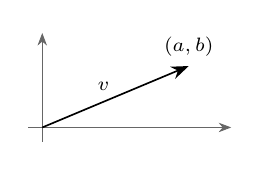
\begin{tikzpicture}[scale=.6]
  \draw[axis] (-.3,0)--(4,0); \draw[axis] (0,-.3)--(0,2);
  \draw[vec] (0,0)--node[above left=-2pt,font=\scriptsize]{$v$} (3.1,1.3);
  \node[above,font=\scriptsize] at (3.1,1.3) {$(a,b)$};
\end{tikzpicture}}{This vector $v$ has norm $\sqrt{a^2+b^2}$.}%
To motivate the concept of inner product, think of vectors in $\R^2$ and $\R^3$
as arrows with initial point at the origin. The length of a vector $v$ in $\R^2$
or $\R^3$ is called the \emph{norm} of $v$ and is denoted by $\norm{v}$. Thus
for $v=(a,b)\in\R^2$, we have
\[ \norm{v} = \sqrt{a^2+b^2}. \]
Similarly, if $v=(a,b,c)\in\R^3$, then $\norm{v}=\sqrt{a^2+b^2+c^2}$.

Even though we cannot draw pictures in higher dimensions, the generalization to
$\R^n$ is easy: we define the norm of $x=(x_1,\dots,x_n)\in\R^n$ by
\[ \norm{x} = \sqrt{x_1^2+\cdots+x_n^2}. \]

The norm is not linear on $\R^n$. To inject linearity into the discussion, we
introduce the dot product.

\begin{definition}[Dot product]\label{ax:6.1}
For $x,y\in\R^n$, the \emph{dot product} of $x$ and $y$, denoted by $x\cdot y$,
is defined by
\[ x\cdot y = x_1y_1+\cdots+x_ny_n, \]
where $x=(x_1,\dots,x_n)$ and $y=(y_1,\dots,y_n)$.
\end{definition}

\marginnote[-4em]{If we think of a vector as a point instead of as an arrow, then
$\norm{x}$ should be interpreted to mean the distance from the origin to the
point $x$.}%
The dot product of two vectors in $\R^n$ is a number, not a vector. Notice that
$x\cdot x=\norm{x}^2$ for all $x\in\R^n$. Furthermore, the dot product on $\R^n$
has the following properties.
\begin{itemize}
\item $x\cdot x\ge0$ for all $x\in\R^n$.
\item $x\cdot x=0$ if and only if $x=0$.
\item For $y\in\R^n$ fixed, the map from $\R^n$ to $\R$ that sends $x\in\R^n$
  to $x\cdot y$ is linear.
\item $x\cdot y=y\cdot x$ for all $x,y\in\R^n$.
\end{itemize}

An inner product is a generalization of the dot product. At this point you may
be tempted to guess that an inner product is defined by abstracting the
properties of the dot product discussed in the last paragraph. For real vector
spaces, that guess is correct. However, so that we can make a definition that
will be useful for both real and complex vector spaces, we need to examine the
complex case before making the definition.

Recall that if $\lambda=a+bi$, where $a,b\in\R$, then
\begin{itemize}
\item the absolute value of $\lambda$, denoted by $\abs{\lambda}$, is defined by
  $\abs{\lambda}=\sqrt{a^2+b^2}$;
\item the complex conjugate of $\lambda$, denoted by $\overline{\lambda}$, is
  defined by $\overline{\lambda}=a-bi$;
\item $\abs{\lambda}^2=\lambda\overline{\lambda}$.
\end{itemize}
See Chapter~4 for the definitions and the basic properties of the absolute value
and complex conjugate.

For $z=(z_1,\dots,z_n)\in\C^n$, we define the norm of $z$ by
\[ \norm{z} = \sqrt{\abs{z_1}^2+\cdots+\abs{z_n}^2}. \]
The absolute values are needed because we want $\norm{z}$ to be a nonnegative
number. Note that
\[ \norm{z}^2 = z_1\overline{z_1}+\cdots+z_n\overline{z_n}. \]

We want to think of $\norm{z}^2$ as the inner product of $z$ with itself, as we
did in $\R^n$. The equation above thus suggests that the inner product of the
vector $w=(w_1,\dots,w_n)\in\C^n$ with $z$ should equal
\[ w_1\overline{z_1}+\cdots+w_n\overline{z_n}. \]
If the roles of the $w$ and $z$ were interchanged, the expression above would be
replaced with its complex conjugate. Thus we should expect that the inner
product of $w$ with $z$ equals the complex conjugate of the inner product of $z$
with $w$. With that motivation, we are now ready to define an inner product on
$V$, which may be a real or a complex vector space.

One comment about the notation used in the next definition:
\begin{itemize}
\item For $\lambda\in\C$, the notation $\lambda\ge0$ means $\lambda$ is real and
  nonnegative.
\end{itemize}

\begin{definition}[Inner product]\label{ax:6.2}
An \emph{inner product} on $V$ is a function that takes each ordered pair
$(u,v)$ of elements of $V$ to a number $\ip{u}{v}\in\F$ and has the following
properties.
\begin{axprops}
\item[positivity] $\ip{v}{v}\ge0$ for all $v\in V$.
\item[definiteness] $\ip{v}{v}=0$ if and only if $v=0$.
\item[additivity in first slot] $\ip{u+v}{w}=\ip{u}{w}+\ip{v}{w}$ for all
  $u,v,w\in V$.
\item[homogeneity in first slot] $\ip{\lambda u}{v}=\lambda\ip{u}{v}$ for all
  $\lambda\in\F$ and all $u,v\in V$.
\item[conjugate symmetry] $\ip{u}{v}=\overline{\ip{v}{u}}$ for all $u,v\in V$.
\end{axprops}
\end{definition}

\marginnote{Most mathematicians define inner products as above, but many
physicists use a definition that requires homogeneity in the second slot
instead of the first slot.}%
Every real number equals its complex conjugate. Thus if we are dealing with a
real vector space, then in the last condition above we can dispense with the
complex conjugate and simply state that $\ip{u}{v}=\ip{v}{u}$ for all
$u,v\in V$.

\begin{example}[Inner products]\label{ax:6.3}\leavevmode
\begin{parts}
\item The \emph{Euclidean inner product} on $\F^n$ is defined by
  \[ \bigl\langle(w_1,\dots,w_n),(z_1,\dots,z_n)\bigr\rangle
     = w_1\overline{z_1}+\cdots+w_n\overline{z_n} \]
  for all $(w_1,\dots,w_n),(z_1,\dots,z_n)\in\F^n$.
\item If $c_1,\dots,c_n$ are positive numbers, then an inner product can be
  defined on $\F^n$ by
  \[ \bigl\langle(w_1,\dots,w_n),(z_1,\dots,z_n)\bigr\rangle
     = c_1w_1\overline{z_1}+\cdots+c_nw_n\overline{z_n} \]
  for all $(w_1,\dots,w_n),(z_1,\dots,z_n)\in\F^n$.
\item An inner product can be defined on the vector space of continuous
  real-valued functions on the interval $[-1,1]$ by
  \[ \ip{f}{g} = \int_{-1}^1 fg \]
  for all $f,g$ continuous real-valued functions on $[-1,1]$.
\item An inner product can be defined on $\Poly(\R)$ by
  \[ \ip{p}{q} = p(0)q(0)+\int_{-1}^1 p'q' \]
  for all $p,q\in\Poly(\R)$.
\item An inner product can be defined on $\Poly(\R)$ by
  \[ \ip{p}{q} = \int_0^\infty p(x)q(x)e^{-x}\,dx \]
  for all $p,q\in\Poly(\R)$.
\end{parts}
\end{example}

\begin{definition}[Inner product space]\label{ax:6.4}
An \emph{inner product space} is a vector space $V$ along with an inner product
on $V$.
\end{definition}

The most important example of an inner product space is $\F^n$ with the
Euclidean inner product given by (a) in the example above. When $\F^n$ is
referred to as an inner product space, you should assume that the inner product
is the Euclidean inner product unless explicitly told otherwise.

So that we do not have to keep repeating the hypothesis that $V$ and $W$ are
inner product spaces, we make the following assumption.

\begin{notation}[$V$, $W$]\label{ax:6.5}
For the rest of this chapter and the next chapter, $V$ and $W$ denote inner
product spaces over $\F$.
\end{notation}

Note the slight abuse of language here. An inner product space is a vector
space along with an inner product on that vector space. When we say that a
vector space $V$ is an inner product space, we are also thinking that an inner
product on $V$ is lurking nearby or is clear from the context (or is the
Euclidean inner product if the vector space is $\F^n$).

\begin{result}[Basic properties of an inner product]\label{ax:6.6}\leavevmode
\begin{parts}
\item For each fixed $v\in V$, the function that takes $u\in V$ to $\ip{u}{v}$
  is a linear map from $V$ to $\F$.
\item $\ip{0}{v}=0$ for every $v\in V$.
\item $\ip{v}{0}=0$ for every $v\in V$.
\item $\ip{u}{v+w}=\ip{u}{v}+\ip{u}{w}$ for all $u,v,w\in V$.
\item $\ip{u}{\lambda v}=\overline{\lambda}\ip{u}{v}$ for all $\lambda\in\F$
  and all $u,v\in V$.
\end{parts}
\end{result}

\begin{proof}\leavevmode
\begin{parts}
\item For $v\in V$, the linearity of $u\mapsto\ip{u}{v}$ follows from the
  conditions of additivity and homogeneity in the first slot in the definition
  of an inner product.
\item Every linear map takes $0$ to $0$. Thus (b) follows from (a).
\item If $v\in V$, then the conjugate symmetry property in the definition of an
  inner product and (b) show that
  $\ip{v}{0}=\overline{\ip{0}{v}}=\overline{0}=0$.
\item Suppose $u,v,w\in V$. Then
  \begin{align*}
  \ip{u}{v+w} &= \overline{\ip{v+w}{u}}\\
    &= \overline{\ip{v}{u}+\ip{w}{u}}\\
    &= \overline{\ip{v}{u}}+\overline{\ip{w}{u}}\\
    &= \ip{u}{v}+\ip{u}{w}.
  \end{align*}
\item Suppose $\lambda\in\F$ and $u,v\in V$. Then
  \begin{align*}
  \ip{u}{\lambda v} &= \overline{\ip{\lambda v}{u}}\\
    &= \overline{\lambda\ip{v}{u}}\\
    &= \overline{\lambda}\,\overline{\ip{v}{u}}\\
    &= \overline{\lambda}\ip{u}{v}. \qedhere
  \end{align*}
\end{parts}
\end{proof}

\subsection{Norms}

Our motivation for defining inner products came initially from the norms of
vectors on $\R^2$ and $\R^3$. Now we see that each inner product determines a
norm.

\begin{definition}[Norm, $\norm{v}$]\label{ax:6.7}
For $v\in V$, the \emph{norm} of $v$, denoted by $\norm{v}$, is defined by
\[ \norm{v} = \sqrt{\ip{v}{v}}. \]
\end{definition}

\begin{example}[Norms]\label{ax:6.8}\leavevmode
\begin{parts}
\item If $(z_1,\dots,z_n)\in\F^n$ (with the Euclidean inner product), then
  \[ \norm{(z_1,\dots,z_n)} = \sqrt{\abs{z_1}^2+\cdots+\abs{z_n}^2}. \]
\item For $f$ in the vector space of continuous real-valued functions on
  $[-1,1]$ and with inner product given as in \ref{ax:6.3}(c), we have
  \[ \norm{f} = \sqrt{\int_{-1}^1 f^2}. \]
\end{parts}
\end{example}

\begin{result}[Basic properties of the norm]\label{ax:6.9}
Suppose $v\in V$.
\begin{parts}
\item $\norm{v}=0$ if and only if $v=0$.
\item $\norm{\lambda v}=\abs{\lambda}\,\norm{v}$ for all $\lambda\in\F$.
\end{parts}
\end{result}

\begin{proof}\leavevmode
\begin{parts}
\item The desired result holds because $\ip{v}{v}=0$ if and only if $v=0$.
\item Suppose $\lambda\in\F$. Then
  \begin{align*}
  \norm{\lambda v}^2 &= \ip{\lambda v}{\lambda v}\\
    &= \lambda\ip{v}{\lambda v}\\
    &= \lambda\overline{\lambda}\ip{v}{v}\\
    &= \abs{\lambda}^2\norm{v}^2.
  \end{align*}
  Taking square roots now gives the desired equality. \qedhere
\end{parts}
\end{proof}

The proof of (b) in the result above illustrates a general principle: working
with norms squared is usually easier than working directly with norms.

Now we come to a crucial definition.

\begin{definition}[Orthogonal]\label{ax:6.10}
Two vectors $u,v\in V$ are called \emph{orthogonal} if $\ip{u}{v}=0$.
\end{definition}

\marginnote{The word \textbf{orthogonal} comes from the Greek word
\textbf{orthogonios}, which means right-angled.}%
In the definition above, the order of the two vectors does not matter, because
$\ip{u}{v}=0$ if and only if $\ip{v}{u}=0$. Instead of saying $u$ and $v$ are
orthogonal, sometimes we say $u$ is orthogonal to $v$.

Exercise~15 asks you to prove that if $u,v$ are nonzero vectors in $\R^2$, then
\[ \ip{u}{v} = \norm{u}\,\norm{v}\cos\theta, \]
where $\theta$ is the angle between $u$ and $v$ (thinking of $u$ and $v$ as
arrows with initial point at the origin). Thus two nonzero vectors in $\R^2$ are
orthogonal (with respect to the Euclidean inner product) if and only if the
cosine of the angle between them is $0$, which happens if and only if the
vectors are perpendicular in the usual sense of plane geometry. Thus you can
think of the word \emph{orthogonal} as a fancy word meaning
\emph{perpendicular}.

We begin our study of orthogonality with an easy result.

\begin{result}[Orthogonality and $0$]\label{ax:6.11}\leavevmode
\begin{parts}
\item $0$ is orthogonal to every vector in $V$.
\item $0$ is the only vector in $V$ that is orthogonal to itself.
\end{parts}
\end{result}

\begin{proof}\leavevmode
\begin{parts}
\item Recall that \ref{ax:6.6}(b) states that $\ip{0}{v}=0$ for every $v\in V$.
\item If $v\in V$ and $\ip{v}{v}=0$, then $v=0$ (by definition of inner
  product). \qedhere
\end{parts}
\end{proof}

For the special case $V=\R^2$, the next theorem was known over 3,500 years ago
in Babylonia and then rediscovered and proved over 2,500 years ago in Greece.
Of course, the proof below is not the original proof.

\begin{result}[Pythagorean theorem]\label{ax:6.12}
Suppose $u,v\in V$. If $u$ and $v$ are orthogonal, then
\[ \norm{u+v}^2 = \norm{u}^2+\norm{v}^2. \]
\end{result}

\begin{proof}
Suppose $\ip{u}{v}=0$. Then
\begin{align*}
\norm{u+v}^2 &= \ip{u+v}{u+v}\\
  &= \ip{u}{u}+\ip{u}{v}+\ip{v}{u}+\ip{v}{v}\\
  &= \norm{u}^2+\norm{v}^2. \qedhere
\end{align*}
\end{proof}

Suppose $u,v\in V$, with $v\ne0$. We would like to write $u$ as a scalar
multiple of $v$ plus a vector $w$ orthogonal to $v$, as suggested in the
picture here.
\begin{center}
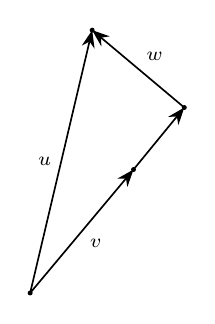
\begin{tikzpicture}[scale=.75]
  \fill (0,0) circle (1.2pt) (1.75,2.09) circle (1.2pt) (2.61,3.14) circle (1.2pt)
    (1.05,4.45) circle (1.2pt);
  \draw[vec] (0,0)--node[below right=-1pt,font=\scriptsize]{$v$} (1.75,2.09);
  \draw[vec] (1.75,2.09)--(2.61,3.14);
  \draw[vec] (0,0)--node[left,font=\scriptsize]{$u$} (1.05,4.45);
  \draw[vec] (2.61,3.14)--node[above right=-1pt,font=\scriptsize]{$w$} (1.05,4.45);
\end{tikzpicture}
\captionof*{figure}{An orthogonal decomposition: $u$ expressed as a scalar
multiple of $v$ plus a vector orthogonal to $v$.}
\end{center}

To discover how to write $u$ as a scalar multiple of $v$ plus a vector
orthogonal to $v$, let $c\in\F$ denote a scalar. Then
\[ u = cv+(u-cv). \]
Thus we need to choose $c$ so that $v$ is orthogonal to $(u-cv)$. Hence we want
\[ 0 = \ip{u-cv}{v} = \ip{u}{v}-c\norm{v}^2. \]
The equation above shows that we should choose $c$ to be
$\ip{u}{v}/\norm{v}^2$. Making this choice of $c$, we can write
\[ u = \frac{\ip{u}{v}}{\norm{v}^2}v
       +\biggl(u-\frac{\ip{u}{v}}{\norm{v}^2}v\biggr). \]
As you should verify, the equation displayed above explicitly writes $u$ as a
scalar multiple of $v$ plus a vector orthogonal to $v$. Thus we have proved the
following key result.

\begin{result}[An orthogonal decomposition]\label{ax:6.13}
Suppose $u,v\in V$, with $v\ne0$. Set
$c=\dfrac{\ip{u}{v}}{\norm{v}^2}$ and
$w=u-\dfrac{\ip{u}{v}}{\norm{v}^2}v$. Then
\[ u=cv+w \quad\text{and}\quad \ip{w}{v}=0. \]
\end{result}

The orthogonal decomposition \ref{ax:6.13} will be used in the proof of the
Cauchy--Schwarz inequality, which is our next result and is one of the most
important inequalities in mathematics.

\begin{result}[Cauchy--Schwarz inequality]\label{ax:6.14}
Suppose $u,v\in V$. Then
\[ \abs{\ip{u}{v}} \le \norm{u}\,\norm{v}. \]
This inequality is an equality if and only if one of $u,v$ is a scalar multiple
of the other.
\end{result}

\begin{proof}
If $v=0$, then both sides of the desired inequality equal $0$. Thus we can
assume that $v\ne0$. Consider the orthogonal decomposition
\[ u = \frac{\ip{u}{v}}{\norm{v}^2}v+w \]
given by \ref{ax:6.13}, where $w$ is orthogonal to $v$. By the Pythagorean
theorem,\axeqstep{ax:6.15}
\begin{align*}
\norm{u}^2 &= \biggl\lVert\frac{\ip{u}{v}}{\norm{v}^2}v\biggr\rVert^2
              +\norm{w}^2\\
  &= \frac{\abs{\ip{u}{v}}^2}{\norm{v}^2}+\norm{w}^2\\
  &\ge \frac{\abs{\ip{u}{v}}^2}{\norm{v}^2}. \axeqtag
\end{align*}
Multiplying both sides of this inequality by $\norm{v}^2$ and then taking
square roots gives the desired inequality.

\marginnote{Augustin-Louis Cauchy (1789--1857) proved \ref{ax:6.16}(a) in 1821.
In 1859, Cauchy's student Viktor Bunyakovsky (1804--1889) proved integral
inequalities like the one in \ref{ax:6.16}(b). A few decades later, similar
discoveries by Hermann Schwarz (1843--1921) attracted more attention and led to
the name of this inequality.}%
The proof in the paragraph above shows that the Cauchy--Schwarz inequality is an
equality if and only if \ref{ax:6.15} is an equality. This happens if and only
if $w=0$. But $w=0$ if and only if $u$ is a multiple of $v$ (see
\ref{ax:6.13}). Thus the Cauchy--Schwarz inequality is an equality if and only
if $u$ is a scalar multiple of $v$ or $v$ is a scalar multiple of $u$ (or both;
the phrasing has been chosen to cover cases in which either $u$ or $v$ equals
$0$).
\end{proof}

\begin{example}[Cauchy--Schwarz inequality]\label{ax:6.16}\leavevmode
\begin{parts}
\item If $x_1,\dots,x_n,y_1,\dots,y_n\in\R$, then
  \[ (x_1y_1+\cdots+x_ny_n)^2 \le (x_1^2+\cdots+x_n^2)(y_1^2+\cdots+y_n^2), \]
  as follows from applying the Cauchy--Schwarz inequality to the vectors
  $(x_1,\dots,x_n),\allowbreak(y_1,\dots,y_n)\in\R^n$, using the usual Euclidean inner
  product.
\item If $f,g$ are continuous real-valued functions on $[-1,1]$, then
  \[ \biggl\lvert\int_{-1}^1 fg\biggr\rvert^2
     \le \biggl(\int_{-1}^1 f^2\biggr)\biggl(\int_{-1}^1 g^2\biggr), \]
  as follows from applying the Cauchy--Schwarz inequality to
  Example~\ref{ax:6.3}(c).
\end{parts}
\end{example}

\marginfig{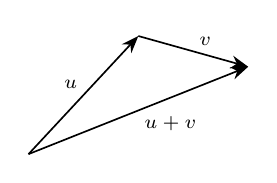
\begin{tikzpicture}[scale=.75]
  \draw[vec] (0,0)--node[above left=-2pt,font=\scriptsize]{$u$} (1.86,2);
  \draw[vec] (1.86,2)--node[above right=-2pt,font=\scriptsize]{$v$} (3.72,1.48);
  \draw[vec] (0,0)--node[below right=-2pt,font=\scriptsize]{$u+v$} (3.72,1.48);
\end{tikzpicture}}{In this triangle, the length of $u+v$ is less than the length
of $u$ plus the length of $v$.}%
The next result, called the triangle inequality, has the geometric
interpretation that the length of each side of a triangle is less than the sum
of the lengths of the other two sides.

Note that the triangle inequality implies that the shortest polygonal path
between two points is a single line segment (a polygonal path consists of line
segments).

\begin{result}[Triangle inequality]\label{ax:6.17}
Suppose $u,v\in V$. Then
\[ \norm{u+v} \le \norm{u}+\norm{v}. \]
This inequality is an equality if and only if one of $u,v$ is a nonnegative
real multiple of the other.
\end{result}

\begin{proof}
We have\axeqstep{ax:6.18}
\begin{align*}
\norm{u+v}^2 &= \ip{u+v}{u+v}\\
  &= \ip{u}{u}+\ip{v}{v}+\ip{u}{v}+\ip{v}{u}\\
  &= \ip{u}{u}+\ip{v}{v}+\ip{u}{v}+\overline{\ip{u}{v}}\\
  &= \norm{u}^2+\norm{v}^2+2\Re\ip{u}{v}\\
  &\le \norm{u}^2+\norm{v}^2+2\abs{\ip{u}{v}} \axeqtag\\
  &\le \norm{u}^2+\norm{v}^2+2\norm{u}\,\norm{v} \refstepcounter{theorem}\axeqtag\label{ax:6.19}\\
  &= (\norm{u}+\norm{v})^2,
\end{align*}
where \ref{ax:6.19} follows from the Cauchy--Schwarz inequality
(\ref{ax:6.14}). Taking square roots of both sides of the inequality above
gives the desired inequality.

The proof above shows that the triangle inequality is an equality if and only
if we have equality in \ref{ax:6.18} and \ref{ax:6.19}. Thus we have equality
in the triangle inequality if and only if\axeqstep{ax:6.20}
\begin{equation*}
\ip{u}{v} = \norm{u}\,\norm{v}. \axeqtag
\end{equation*}
If one of $u,v$ is a nonnegative real multiple of the other, then
\ref{ax:6.20} holds. Conversely, suppose \ref{ax:6.20} holds. Then the
condition for equality in the Cauchy--Schwarz inequality (\ref{ax:6.14})
implies that one of $u,v$ is a scalar multiple of the other. This scalar must
be a nonnegative real number, by \ref{ax:6.20}, completing the proof.
\end{proof}

For the reverse triangle inequality, see Exercise~20.

\marginfig[-24mm]{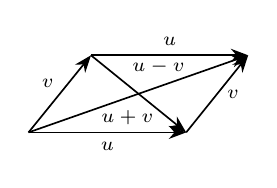
\begin{tikzpicture}[scale=.62]
  \draw[vec] (0,0)--node[above left=-2pt,font=\scriptsize]{$v$} (1.28,1.58);
  \draw[vec] (1.28,1.58)--node[above,font=\scriptsize]{$u$} (4.5,1.58);
  \draw[vec] (0,0)--node[below,font=\scriptsize]{$u$} (3.23,0);
  \draw[vec] (3.23,0)--node[right,font=\scriptsize]{$v$} (4.5,1.58);
  \draw[vec] (0,0)--node[below=1pt,pos=.45,font=\scriptsize]{$u+v$} (4.5,1.58);
  \draw[vec] (1.28,1.58)--node[above right=-1pt,pos=.35,font=\scriptsize]{$u-v$}
    (3.23,0);
\end{tikzpicture}}{The diagonals of this parallelogram are $u+v$ and $u-v$.}%
The next result is called the parallelogram equality because of its geometric
interpretation: in every parallelogram, the sum of the squares of the lengths
of the diagonals equals the sum of the squares of the lengths of the four
sides. Note that the proof here is more straightforward than the usual proof in
Euclidean geometry.

\begin{result}[Parallelogram equality]\label{ax:6.21}
Suppose $u,v\in V$. Then
\[ \norm{u+v}^2+\norm{u-v}^2 = 2(\norm{u}^2+\norm{v}^2). \]
\end{result}

\begin{proof}
We have
\begin{align*}
\norm{u+v}^2+\norm{u-v}^2 &= \ip{u+v}{u+v}+\ip{u-v}{u-v}\\
  &= \norm{u}^2+\norm{v}^2+\ip{u}{v}+\ip{v}{u}\\
  &\qquad+\norm{u}^2+\norm{v}^2-\ip{u}{v}-\ip{v}{u}\\
  &= 2(\norm{u}^2+\norm{v}^2),
\end{align*}
as desired.
\end{proof}

% ------------------------------------------------------------------ exercises
\exercisesheading{6A}

\begin{exercise}
Prove or give a counterexample: If $v_1,\dots,v_m\in V$, then
\[ \sum_{j=1}^m\sum_{k=1}^m\ip{v_j}{v_k} \ge 0. \]
\end{exercise}

\begin{exercise}
Suppose $S\in\Lin(V)$. Define $\ip{\cdot}{\cdot}_1$ by
\[ \ip{u}{v}_1 = \ip{Su}{Sv} \]
for all $u,v\in V$. Show that $\ip{\cdot}{\cdot}_1$ is an inner product on $V$
if and only if $S$ is injective.
\end{exercise}

\begin{exercise}\leavevmode
\begin{parts}
\item Show that the function taking an ordered pair
  $\bigl((x_1,x_2),(y_1,y_2)\bigr)$ of elements of $\R^2$ to
  $\abs{x_1y_1}+\abs{x_2y_2}$ is not an inner product on $\R^2$.
\item Show that the function taking an ordered pair
  $\bigl((x_1,x_2,x_3),(y_1,y_2,y_3)\bigr)$ of elements of $\R^3$ to
  $x_1y_1+x_3y_3$ is not an inner product on $\R^3$.
\end{parts}
\end{exercise}

\begin{exercise}
Suppose $T\in\Lin(V)$ is such that $\norm{Tv}\le\norm{v}$ for every $v\in V$.
Prove that $T-\sqrt2\,I$ is injective.
\end{exercise}

\begin{exercise}
Suppose $V$ is a real inner product space.
\begin{parts}
\item Show that $\ip{u+v}{u-v}=\norm{u}^2-\norm{v}^2$ for every $u,v\in V$.
\item Show that if $u,v\in V$ have the same norm, then $u+v$ is orthogonal to
  $u-v$.
\item Use (b) to show that the diagonals of a rhombus are perpendicular to each
  other.
\end{parts}
\end{exercise}

\begin{exercise}
Suppose $u,v\in V$. Prove that
$\ip{u}{v}=0 \iff \norm{u}\le\norm{u+av}$ for all $a\in\F$.
\end{exercise}

\begin{exercise}
Suppose $u,v\in V$. Prove that $\norm{au+bv}=\norm{bu+av}$ for all $a,b\in\R$
if and only if $\norm{u}=\norm{v}$.
\end{exercise}

\begin{exercise}
Suppose $a,b,c,x,y\in\R$ and $a^2+b^2+c^2+x^2+y^2\le1$. Prove that
$a+b+c+4x+9y\le10$.
\end{exercise}

\begin{exercise}
Suppose $u,v\in V$ and $\norm{u}=\norm{v}=1$ and $\ip{u}{v}=1$. Prove that
$u=v$.
\end{exercise}

\begin{exercise}
Suppose $u,v\in V$ and $\norm{u}\le1$ and $\norm{v}\le1$. Prove that
\[ \sqrt{1-\norm{u}^2}\,\sqrt{1-\norm{v}^2} \le 1-\abs{\ip{u}{v}}. \]
\end{exercise}

\begin{exercise}
Find vectors $u,v\in\R^2$ such that $u$ is a scalar multiple of $(1,3)$, $v$ is
orthogonal to $(1,3)$, and $(1,2)=u+v$.
\end{exercise}

\begin{exercise}
Suppose $a,b,c,d$ are positive numbers.
\begin{parts}
\item Prove that
  $(a+b+c+d)\Bigl(\dfrac1a+\dfrac1b+\dfrac1c+\dfrac1d\Bigr)\ge16$.
\item For which positive numbers $a,b,c,d$ is the inequality above an equality?
\end{parts}
\end{exercise}

\begin{exercise}
Show that the square of an average is less than or equal to the average of the
squares. More precisely, show that if $a_1,\dots,a_n\in\R$, then the square of
the average of $a_1,\dots,a_n$ is less than or equal to the average of
$a_1^2,\dots,a_n^2$.
\end{exercise}

\begin{exercise}
Suppose $v\in V$ and $v\ne0$. Prove that $v/\norm{v}$ is the unique closest
element on the unit sphere of $V$ to $v$. More precisely, prove that if $u\in V$
and $\norm{u}=1$, then
\[ \biggl\lVert v-\frac{v}{\norm{v}}\biggr\rVert \le \norm{v-u}, \]
with equality only if $u=v/\norm{v}$.
\end{exercise}

\begin{exercise}
Suppose $u,v$ are nonzero vectors in $\R^2$. Prove that
\[ \ip{u}{v} = \norm{u}\,\norm{v}\cos\theta, \]
where $\theta$ is the angle between $u$ and $v$ (thinking of $u$ and $v$ as
arrows with initial point at the origin).
\exnote{Hint: Use the law of cosines on the triangle formed by $u$, $v$, and
$u-v$.}
\end{exercise}

\begin{exercise}
The angle between two vectors (thought of as arrows with initial point at the
origin) in $\R^2$ or $\R^3$ can be defined geometrically. However, geometry is
not as clear in $\R^n$ for $n>3$. Thus the angle between two nonzero vectors
$x,y\in\R^n$ is defined to be
\[ \arccos\frac{\ip{x}{y}}{\norm{x}\,\norm{y}}, \]
where the motivation for this definition comes from Exercise~15. Explain why the
Cauchy--Schwarz inequality is needed to show that this definition makes sense.
\end{exercise}

\begin{exercise}
Prove that
\[ \biggl(\sum_{k=1}^n a_kb_k\biggr)^2
   \le \biggl(\sum_{k=1}^n ka_k^2\biggr)\biggl(\sum_{k=1}^n\frac{b_k^2}{k}\biggr) \]
for all real numbers $a_1,\dots,a_n$ and $b_1,\dots,b_n$.
\end{exercise}

\begin{exercise}\leavevmode
\begin{parts}
\item Suppose $f\colon[1,\infty)\to[0,\infty)$ is continuous. Show that
  \[ \biggl(\int_1^\infty f\biggr)^2 \le \int_1^\infty x^2\bigl(f(x)\bigr)^2\,dx. \]
\item For which continuous functions $f\colon[1,\infty)\to[0,\infty)$ is the
  inequality in (a) an equality with both sides finite?
\end{parts}
\end{exercise}

\begin{exercise}
Suppose $v_1,\dots,v_n$ is a basis of $V$ and $T\in\Lin(V)$. Prove that if
$\lambda$ is an eigenvalue of $T$, then
\[ \abs{\lambda}^2 \le \sum_{j=1}^n\sum_{k=1}^n\abs{\Mat(T)_{j,k}}^2, \]
where $\Mat(T)_{j,k}$ denotes the entry in row $j$, column $k$ of the matrix of
$T$ with respect to the basis $v_1,\dots,v_n$.
\end{exercise}

\begin{exercise}
Prove that if $u,v\in V$, then
$\bigl\lvert\,\norm{u}-\norm{v}\,\bigr\rvert\le\norm{u-v}$.
\exnote{The inequality above is called the \textbf{reverse triangle
inequality}. For the reverse triangle inequality when $V=\C$, see Exercise~2 in
Chapter~4.}
\end{exercise}

\begin{exercise}
Suppose $u,v\in V$ are such that
\[ \norm{u}=3, \qquad \norm{u+v}=4, \qquad \norm{u-v}=6. \]
What number does $\norm{v}$ equal?
\end{exercise}

\begin{exercise}
Show that if $u,v\in V$, then
\[ \norm{u+v}\,\norm{u-v} \le \norm{u}^2+\norm{v}^2. \]
\end{exercise}

\begin{exercise}
Suppose $v_1,\dots,v_m\in V$ are such that $\norm{v_k}\le1$ for each
$k=1,\dots,m$. Show that there exist $a_1,\dots,a_m\in\{1,-1\}$ such that
\[ \norm{a_1v_1+\cdots+a_mv_m} \le \sqrt{m}. \]
\end{exercise}

\begin{exercise}
Prove or give a counterexample: If $\norm{\cdot}$ is the norm associated with an
inner product on $\R^2$, then there exists $(x,y)\in\R^2$ such that
$\norm{(x,y)}\ne\max\{\abs{x},\abs{y}\}$.
\end{exercise}

\begin{exercise}
Suppose $p>0$. Prove that there is an inner product on $\R^2$ such that the
associated norm is given by
\[ \norm{(x,y)} = (\abs{x}^p+\abs{y}^p)^{1/p} \]
for all $(x,y)\in\R^2$ if and only if $p=2$.
\end{exercise}

\begin{exercise}
Suppose $V$ is a real inner product space. Prove that
\[ \ip{u}{v} = \frac{\norm{u+v}^2-\norm{u-v}^2}{4} \]
for all $u,v\in V$.
\end{exercise}

\begin{exercise}
Suppose $V$ is a complex inner product space. Prove that
\[ \ip{u}{v} = \frac{\norm{u+v}^2-\norm{u-v}^2+\norm{u+iv}^2i
   -\norm{u-iv}^2i}{4} \]
for all $u,v\in V$.
\end{exercise}

\begin{exercise}
A norm on a vector space $U$ is a function
\[ \norm{\cdot}\colon U\to[0,\infty) \]
such that $\norm{u}=0$ if and only if $u=0$, $\norm{\alpha u}=\abs{\alpha}\norm{u}$
for all $\alpha\in\F$ and all $u\in U$, and $\norm{u+v}\le\norm{u}+\norm{v}$
for all $u,v\in U$. Prove that a norm satisfying the parallelogram equality
comes from an inner product (in other words, show that if $\norm{\cdot}$ is a
norm on $U$ satisfying the parallelogram equality, then there is an inner
product $\ip{\cdot}{\cdot}$ on $U$ such that $\norm{u}=\ip{u}{u}^{1/2}$ for all
$u\in U$).
\end{exercise}

\begin{exercise}
Suppose $V_1,\dots,V_m$ are inner product spaces. Show that the equation
\[ \bigl\langle(u_1,\dots,u_m),(v_1,\dots,v_m)\bigr\rangle
   = \ip{u_1}{v_1}+\cdots+\ip{u_m}{v_m} \]
defines an inner product on $V_1\times\cdots\times V_m$.
\exnote{In the expression above on the right, for each $k=1,\dots,m$, the inner
product $\ip{u_k}{v_k}$ denotes the inner product on $V_k$. Each of the spaces
$V_1,\dots,V_m$ may have a different inner product, even though the same
notation is used here.}
\end{exercise}

\begin{exercise}
Suppose $V$ is a real inner product space. For $u,v,w,x\in V$, define
\[ \ip{u+iv}{w+ix}_\C = \ip{u}{w}+\ip{v}{x}+(\ip{v}{w}-\ip{u}{x})i. \]
\begin{parts}
\item Show that $\ip{\cdot}{\cdot}_\C$ makes $V_\C$ into a complex inner product
  space.
\item Show that if $u,v\in V$, then
  \[ \ip{u}{v}_\C = \ip{u}{v} \quad\text{and}\quad
     \norm{u+iv}_\C^2 = \norm{u}^2+\norm{v}^2. \]
\end{parts}
\exnote{See Exercise~8 in Section~1B for the definition of the complexification
$V_\C$.}
\end{exercise}

\begin{exercise}
Suppose $u,v,w\in V$. Prove that
\[ \bigl\lVert w-(1/2)(u+v)\bigr\rVert^2
   = \frac{\norm{w-u}^2+\norm{w-v}^2}{2}-\frac{\norm{u-v}^2}{4}. \]
\end{exercise}

\begin{exercise}
Suppose that $E$ is a subset of $V$ with the property that $u,v\in E$ implies
$(1/2)(u+v)\in E$. Let $w\in V$. Show that there is at most one point in $E$
that is closest to $w$. In other words, show that there is at most one $u\in E$
such that
\[ \norm{w-u} \le \norm{w-x} \]
for all $x\in E$.
\end{exercise}

\begin{exercise}
Suppose $f,g$ are differentiable functions from $\R$ to $\R^n$.
\begin{parts}
\item Show that
  \[ \bigl\langle f(t),g(t)\bigr\rangle'
     = \bigl\langle f'(t),g(t)\bigr\rangle+\bigl\langle f(t),g'(t)\bigr\rangle. \]
\item Suppose $c$ is a positive number and $\norm{f(t)}=c$ for every $t\in\R$.
  Show that $\bigl\langle f'(t),f(t)\bigr\rangle=0$ for every $t\in\R$.
\item Interpret the result in (b) geometrically in terms of the tangent vector
  to a curve lying on a sphere in $\R^n$ centered at the origin.
\end{parts}
\exnote{A function $f\colon\R\to\R^n$ is called differentiable if there exist
differentiable functions $f_1,\dots,f_n$ from $\R$ to $\R$ such that
$f(t)=\bigl(f_1(t),\dots,f_n(t)\bigr)$ for each $t\in\R$. Furthermore, for each
$t\in\R$, the derivative $f'(t)\in\R^n$ is defined by
$f'(t)=\bigl(f_1'(t),\dots,f_n'(t)\bigr)$.}
\end{exercise}

\begin{exercise}
Use inner products to prove Apollonius's identity: In a triangle with sides of
length $a$, $b$, and $c$, let $d$ be the length of the line segment from the
midpoint of the side of length $c$ to the opposite vertex. Then
\[ a^2+b^2 = 1/2c^2+2d^2. \]
\begin{center}
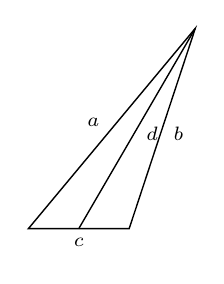
\begin{tikzpicture}[scale=.8]
  \draw[line width=.5pt] (0,0)--(1.6,0)--(2.65,3.18)--cycle;
  \draw[line width=.5pt] (.8,0)--(2.65,3.18);
  \node[font=\scriptsize,above left=-1pt] at (1.25,1.5) {$a$};
  \node[font=\scriptsize,right] at (1.72,1.5) {$d$};
  \node[font=\scriptsize,right] at (2.15,1.5) {$b$};
  \node[font=\scriptsize,below] at (.8,0) {$c$};
\end{tikzpicture}
\end{center}
\end{exercise}

\begin{exercise}
Fix a positive integer $n$. The \emph{Laplacian} $\Delta p$ of a twice
differentiable real-valued function $p$ on $\R^n$ is the function on $\R^n$
defined by
\[ \Delta p = \frac{\partial^2p}{\partial x_1^2}+\cdots
   +\frac{\partial^2p}{\partial x_n^2}. \]
The function $p$ is called \emph{harmonic} if $\Delta p=0$.

A \emph{polynomial} on $\R^n$ is a linear combination (with coefficients in
$\R$) of functions of the form $x_1^{m_1}\cdots x_n^{m_n}$, where
$m_1,\dots,m_n$ are nonnegative integers.

Suppose $q$ is a polynomial on $\R^n$. Prove that there exists a harmonic
polynomial $p$ on $\R^n$ such that $p(x)=q(x)$ for every $x\in\R^n$ with
$\norm{x}=1$.
\exnote{The only fact about harmonic functions that you need for this exercise
is that if $p$ is a harmonic function on $\R^n$ and $p(x)=0$ for all
$x\in\R^n$ with $\norm{x}=1$, then $p=0$.}
\exnote{Hint: A reasonable guess is that the desired harmonic polynomial $p$ is
of the form $q+(1-\norm{x}^2)r$ for some polynomial $r$. Prove that there is a
polynomial $r$ on $\R^n$ such that $q+(1-\norm{x}^2)r$ is harmonic by defining
an operator $T$ on a suitable vector space by
\[ Tr = \Delta\bigl((1-\norm{x}^2)r\bigr) \]
and then showing that $T$ is injective and hence surjective.}
\end{exercise}

\axquote{In realms of numbers, where the secrets lie,\\
A noble truth emerges from the deep,\\
Cauchy and Schwarz, their wisdom they apply,\\
An inequality for all to keep.\par
Two vectors, by this bond, are intertwined,\\
As inner products weave a gilded thread,\\
Their magnitude, by providence, confined,\\
A bound to which their destiny is wed.\par
Though shadows fall, and twilight dims the day,\\
This inequality will stand the test,\\
To guide us in our quest, to light the way,\\
And in its truth, our understanding rest.\par
So sing, ye muses, of this noble feat,\\
Cauchy--Schwarz, the bound that none can beat.}{written by ChatGPT with input
\emph{Shakespearean sonnet on Cauchy--Schwarz inequality}}

\iftestbuild % TEST-ONLY-BEGIN
\setcounter{section}{1}\setcounter{theorem}{21}
\fi % TEST-ONLY-END
% Source: book pp. 197--210 (PDF 211--224); no solutions for this section.
\section{Orthonormal Bases}

\subsection{Orthonormal Lists and the Gram--Schmidt Procedure}

\begin{definition}[Orthonormal]\label{ax:6.22}\leavevmode
\begin{itemize}
\item A list of vectors is called \emph{orthonormal} if each vector in the list
  has norm $1$ and is orthogonal to all the other vectors in the list.
\item In other words, a list $e_1,\dots,e_m$ of vectors in $V$ is orthonormal if
  \[ \ip{e_j}{e_k} = \begin{cases} 1 & \text{if } j=k,\\
                                   0 & \text{if } j\ne k \end{cases} \]
  for all $j,k\in\{1,\dots,m\}$.
\end{itemize}
\end{definition}

\begin{example}[Orthonormal lists]\label{ax:6.23}\leavevmode
\begin{parts}
\item The standard basis of $\F^n$ is an orthonormal list.
\item $\bigl(1/\sqrt3,1/\sqrt3,1/\sqrt3\bigr),
  \bigl(-1/\sqrt2,1/\sqrt2,0\bigr)$ is an orthonormal list
  in $\F^3$.
\item $\bigl(1/\sqrt3,1/\sqrt3,1/\sqrt3\bigr),
  \bigl(-1/\sqrt2,1/\sqrt2,0\bigr),
  \bigl(1/\sqrt6,1/\sqrt6,-2/\sqrt6\bigr)$ is an
  orthonormal list in $\F^3$.
\item Suppose $n$ is a positive integer. Then, as Exercise~4 asks you to verify,
  \[ \frac{1}{\sqrt{2\pi}}, \frac{\cos x}{\sqrt\pi}, \frac{\cos 2x}{\sqrt\pi},
     \dots, \frac{\cos nx}{\sqrt\pi}, \frac{\sin x}{\sqrt\pi},
     \frac{\sin 2x}{\sqrt\pi}, \dots, \frac{\sin nx}{\sqrt\pi} \]
  is an orthonormal list of vectors in $C[-\pi,\pi]$, the vector space of
  continuous real-valued functions on $[-\pi,\pi]$ with inner product
  \[ \ip{f}{g} = \int_{-\pi}^{\pi} fg. \]
  The orthonormal list above is often used for modeling periodic phenomena,
  such as tides.
\item Suppose we make $\Poly_2(\R)$ into an inner product space using the inner
  product given by
  \[ \ip{p}{q} = \int_{-1}^{1} pq \]
  for all $p,q\in\Poly_2(\R)$. The standard basis $1,x,x^2$ of $\Poly_2(\R)$ is
  not an orthonormal list because the vectors in that list do not have norm $1$.
  Dividing each vector by its norm gives the list $1/\sqrt2$,
  $\sqrt{3/2}\,x$, $\sqrt{5/2}\,x^2$, in which each vector has norm $1$, and the
  second vector is orthogonal to the first and third vectors. However, the
  first and third vectors are not orthogonal. Thus this is not an orthonormal
  list. Soon we will see how to construct an orthonormal list from the standard
  basis $1,x,x^2$ (see Example~\ref{ax:6.34}).
\end{parts}
\end{example}

Orthonormal lists are particularly easy to work with, as illustrated by the
next result.

\begin{result}[Norm of an orthonormal linear combination]\label{ax:6.24}
Suppose $e_1,\dots,e_m$ is an orthonormal list of vectors in $V$. Then
\[ \norm{a_1e_1+\cdots+a_me_m}^2 = \abs{a_1}^2+\cdots+\abs{a_m}^2 \]
for all $a_1,\dots,a_m\in\F$.
\end{result}

\begin{proof}
Because each $e_k$ has norm $1$, this follows from repeated applications of the
Pythagorean theorem (\ref{ax:6.12}).
\end{proof}

The result above has the following important corollary.

\begin{result}[Orthonormal lists are linearly independent]\label{ax:6.25}
Every orthonormal list of vectors is linearly independent.
\end{result}

\begin{proof}
Suppose $e_1,\dots,e_m$ is an orthonormal list of vectors in $V$ and
$a_1,\dots,a_m\in\F$ are such that
\[ a_1e_1+\cdots+a_me_m = 0. \]
Then $\abs{a_1}^2+\cdots+\abs{a_m}^2=0$ (by \ref{ax:6.24}), which means that all
the $a_k$'s are $0$. Thus $e_1,\dots,e_m$ is linearly independent.
\end{proof}

Now we come to an important inequality.

\begin{result}[Bessel's inequality]\label{ax:6.26}
Suppose $e_1,\dots,e_m$ is an orthonormal list of vectors in $V$. If $v\in V$
then
\[ \abs{\ip{v}{e_1}}^2+\cdots+\abs{\ip{v}{e_m}}^2 \le \norm{v}^2. \]
\end{result}

\begin{proof}
Suppose $v\in V$. Then
\[ v = \underbrace{\ip{v}{e_1}e_1+\cdots+\ip{v}{e_m}e_m}_{u}
     + \underbrace{v-\ip{v}{e_1}e_1-\cdots-\ip{v}{e_m}e_m}_{w}. \]

Let $u$ and $w$ be defined as in the equation above. If $k\in\{1,\dots,m\}$, then
$\ip{w}{e_k}=\ip{v}{e_k}-\ip{v}{e_k}\ip{e_k}{e_k}=0$. This implies that
$\ip{w}{u}=0$. The Pythagorean theorem now implies that
\begin{align*}
\norm{v}^2 &= \norm{u}^2+\norm{w}^2\\
           &\ge \norm{u}^2\\
           &= \abs{\ip{v}{e_1}}^2+\cdots+\abs{\ip{v}{e_m}}^2,
\end{align*}
where the last line comes from \ref{ax:6.24}.
\end{proof}

The next definition introduces one of the most useful concepts in the study of
inner product spaces.

\begin{definition}[Orthonormal basis]\label{ax:6.27}
An \emph{orthonormal basis} of $V$ is an orthonormal list of vectors in $V$ that
is also a basis of $V$.
\end{definition}

For example, the standard basis is an orthonormal basis of $\F^n$.

\begin{result}[Orthonormal lists of the right length are orthonormal
bases]\label{ax:6.28}
Suppose $V$ is finite-dimensional. Then every orthonormal list of vectors in $V$
of length $\dim V$ is an orthonormal basis of $V$.
\end{result}

\begin{proof}
By \ref{ax:6.25}, every orthonormal list of vectors in $V$ is linearly
independent. Thus every such list of the right length is a basis---see
\ref{ax:2.38}.
\end{proof}

\begin{example}[An orthonormal basis of $\F^4$]\label{ax:6.29}
As mentioned above, the standard basis is an orthonormal basis of $\F^4$. We now
show that
\[ (1/2,1/2,1/2,1/2),
   (1/2,1/2,-1/2,-1/2),
   (1/2,-1/2,-1/2,1/2),
   (-1/2,1/2,-1/2,1/2) \]
is also an orthonormal basis of $\F^4$.

We have
\[ \bigl\lVert(1/2,1/2,1/2,1/2)\bigr\rVert
   = \sqrt{1/2^2+1/2^2+1/2^2+1/2^2} = 1. \]
Similarly, the other three vectors in the list above also have norm $1$.

Note that
\[ \bigl\langle(1/2,1/2,1/2,1/2),(1/2,1/2,-1/2,-1/2)\bigr\rangle
   = 1/2\cdot1/2+1/2\cdot1/2+1/2\cdot(-1/2)+1/2\cdot(-1/2) = 0. \]
Similarly, the inner product of any two distinct vectors in the list above also
equals $0$.

Thus the list above is orthonormal. Because we have an orthonormal list of
length four in the four-dimensional vector space $\F^4$, this list is an
orthonormal basis of $\F^4$ (by \ref{ax:6.28}).
\end{example}

In general, given a basis $e_1,\dots,e_n$ of $V$ and a vector $v\in V$, we know
that there is some choice of scalars $a_1,\dots,a_n\in\F$ such that
\[ v = a_1e_1+\cdots+a_ne_n. \]
Computing the numbers $a_1,\dots,a_n$ that satisfy the equation above can be a
long computation for an arbitrary basis of $V$. The next result shows, however,
that this is easy for an orthonormal basis---just take $a_k=\ip{v}{e_k}$.

\marginnote{The formula below for $\norm{v}$ is called Parseval's
identity. It was published in 1799 in the context of Fourier series.}%
Notice how the next result makes each inner product space of dimension $n$
behave like $\F^n$, with the role of the coordinates of a vector in $\F^n$
played by $\ip{v}{e_1},\dots,\ip{v}{e_n}$.

\begin{result}[Writing a vector as a linear combination of an orthonormal
basis]\label{ax:6.30}
Suppose $e_1,\dots,e_n$ is an orthonormal basis of $V$ and $u,v\in V$. Then
\begin{parts}
\item $v=\ip{v}{e_1}e_1+\cdots+\ip{v}{e_n}e_n$;
\item $\norm{v}^2=\abs{\ip{v}{e_1}}^2+\cdots+\abs{\ip{v}{e_n}}^2$;
\item $\ip{u}{v}=\ip{u}{e_1}\overline{\ip{v}{e_1}}+\cdots
  +\ip{u}{e_n}\overline{\ip{v}{e_n}}$.
\end{parts}
\end{result}

\begin{proof}
Because $e_1,\dots,e_n$ is a basis of $V$, there exist scalars $a_1,\dots,a_n$
such that
\[ v = a_1e_1+\cdots+a_ne_n. \]
Because $e_1,\dots,e_n$ is orthonormal, taking the inner product of both sides of
this equation with $e_k$ gives $\ip{v}{e_k}=a_k$. Thus (a) holds.

Now (b) follows immediately from (a) and \ref{ax:6.24}.

Take the inner product of $u$ with each side of (a) and then get (c) by using
conjugate linearity [\ref{ax:6.6}(d) and \ref{ax:6.6}(e)] in the second slot of
the inner product.
\end{proof}

\begin{example}[Finding coefficients for a linear combination]\label{ax:6.31}
Suppose we want to write the vector $(1,2,4,7)\in\F^4$ as a linear combination
of the orthonormal basis
\[ (1/2,1/2,1/2,1/2),
   (1/2,1/2,-1/2,-1/2),
   (1/2,-1/2,-1/2,1/2),
   (-1/2,1/2,-1/2,1/2) \]
of $\F^4$ from Example~\ref{ax:6.29}. Instead of solving a system of four linear
equations in four unknowns, as typically would be required if we were working
with a nonorthonormal basis, we simply evaluate four inner products and use
\ref{ax:6.30}(a), getting that $(1,2,4,7)$ equals
\[ 7(1/2,1/2,1/2,1/2)
   -4(1/2,1/2,-1/2,-1/2)
   +(1/2,-1/2,-1/2,1/2)
   +2(-1/2,1/2,-1/2,1/2). \]
\end{example}

Now that we understand the usefulness of orthonormal bases, how do we go about
finding them? For example, does $\Poly_m(\R)$ with inner product as in
\ref{ax:6.3}(c) have an orthonormal basis? The next result will lead to answers
to these questions.

\marginnote{J\o rgen Gram (1850--1916) and Erhard Schmidt (1876--1959)
popularized this algorithm that constructs orthonormal lists.}%
The algorithm used in the next proof is called the \emph{Gram--Schmidt
procedure}. It gives a method for turning a linearly independent list into an
orthonormal list with the same span as the original list.

\begin{result}[Gram--Schmidt procedure]\label{ax:6.32}
Suppose $v_1,\dots,v_m$ is a linearly independent list of vectors in $V$. Let
$f_1=v_1$. For $k=2,\dots,m$, define $f_k$ inductively by
\[ f_k = v_k-\frac{\ip{v_k}{f_1}}{\norm{f_1}^2}f_1-\cdots
         -\frac{\ip{v_k}{f_{k-1}}}{\norm{f_{k-1}}^2}f_{k-1}. \]
For each $k=1,\dots,m$, let $e_k=\dfrac{f_k}{\norm{f_k}}$. Then
$e_1,\dots,e_m$ is an orthonormal list of vectors in $V$ such that
\[ \spn(v_1,\dots,v_k) = \spn(e_1,\dots,e_k) \]
for each $k=1,\dots,m$.
\end{result}

\begin{proof}
We will show by induction on $k$ that the desired conclusion holds. To get
started with $k=1$, note that because $e_1=f_1/\norm{f_1}$, we have
$\norm{e_1}=1$; also, $\spn(v_1)=\spn(e_1)$ because $e_1$ is a nonzero multiple
of $v_1$.

Suppose $1<k\le m$ and the list $e_1,\dots,e_{k-1}$ generated by \ref{ax:6.32}
is an orthonormal list such that\refstepcounter{theorem}\label{ax:6.33}
\[ \spn(v_1,\dots,v_{k-1}) = \spn(e_1,\dots,e_{k-1}). \tag*{\thetheorem} \]
Because $v_1,\dots,v_m$ is linearly independent, we have
$v_k\notin\spn(v_1,\dots,v_{k-1})$. Thus
$v_k\notin\spn(e_1,\dots,e_{k-1})=\spn(f_1,\dots,f_{k-1})$, which implies that
$f_k\ne0$. Hence we are not dividing by $0$ in the definition of $e_k$ given in
\ref{ax:6.32}. Dividing a vector by its norm produces a new vector with
norm $1$; thus $\norm{e_k}=1$.

Let $j\in\{1,\dots,k-1\}$. Then
\begin{align*}
\ip{e_k}{e_j}
  &= \frac{1}{\norm{f_k}\,\norm{f_j}}\ip{f_k}{f_j}\\
  &= \frac{1}{\norm{f_k}\,\norm{f_j}}
     \biggl\langle v_k-\frac{\ip{v_k}{f_1}}{\norm{f_1}^2}f_1-\cdots
     -\frac{\ip{v_k}{f_{k-1}}}{\norm{f_{k-1}}^2}f_{k-1}, f_j\biggr\rangle\\
  &= \frac{1}{\norm{f_k}\,\norm{f_j}}(\ip{v_k}{f_j}-\ip{v_k}{f_j})\\
  &= 0.
\end{align*}
Thus $e_1,\dots,e_k$ is an orthonormal list.

From the definition of $e_k$ given in \ref{ax:6.32}, we see that
$v_k\in\spn(e_1,\dots,e_k)$. Combining this information with \ref{ax:6.33}
shows that
\[ \spn(v_1,\dots,v_k) \subseteq \spn(e_1,\dots,e_k). \]
Both lists above are linearly independent (the $v$'s by hypothesis, and the
$e$'s by orthonormality and \ref{ax:6.25}). Thus both subspaces above have
dimension $k$, and hence they are equal, completing the induction step and thus
completing the proof.
\end{proof}

\begin{example}[An orthonormal basis of $\Poly_2(\R)$]\label{ax:6.34}
Suppose we make $\Poly_2(\R)$ into an inner product space using the inner product
given by
\[ \ip{p}{q} = \int_{-1}^{1} pq \]
for all $p,q\in\Poly_2(\R)$. We know that $1,x,x^2$ is a basis of $\Poly_2(\R)$,
but it is not an orthonormal basis. We will find an orthonormal basis of
$\Poly_2(\R)$ by applying the Gram--Schmidt procedure with $v_1=1$, $v_2=x$,
and $v_3=x^2$.

To get started, take $f_1=v_1=1$. Thus $\norm{f_1}^2=\int_{-1}^{1}1=2$. Hence
the formula in \ref{ax:6.32} tells us that
\[ f_2 = v_2-\frac{\ip{v_2}{f_1}}{\norm{f_1}^2}f_1
       = x-\frac{\ip{x}{1}}{\norm{f_1}^2} = x, \]
where the last equality holds because $\ip{x}{1}=\int_{-1}^{1}t\,dt=0$.

The formula above for $f_2$ implies that
$\norm{f_2}^2=\int_{-1}^{1}t^2\,dt=2/3$. Now the formula in \ref{ax:6.32}
tells us that
\[ f_3 = v_3-\frac{\ip{v_3}{f_1}}{\norm{f_1}^2}f_1
            -\frac{\ip{v_3}{f_2}}{\norm{f_2}^2}f_2
       = x^2-1/2\ip{x^2}{1}-3/2\ip{x^2}{x}x = x^2-1/3. \]

The formula above for $f_3$ implies that
\[ \norm{f_3}^2 = \int_{-1}^{1}(t^2-1/3)^2\,dt
   = \int_{-1}^{1}(t^4-2/3t^2+1/9)\,dt = 8/45. \]

Now dividing each of $f_1,f_2,f_3$ by its norm gives us the orthonormal list
\[ \sqrt{1/2},\ \sqrt{3/2}\,x,\
   \sqrt{45/8}(x^2-1/3). \]
The orthonormal list above has length three, which is the dimension of
$\Poly_2(\R)$. Hence this orthonormal list is an orthonormal basis of
$\Poly_2(\R)$ [by \ref{ax:6.28}].
\end{example}

Now we can answer the question about the existence of orthonormal bases.

\begin{result}[Existence of orthonormal basis]\label{ax:6.35}
Every finite-dimensional inner product space has an orthonormal basis.
\end{result}

\begin{proof}
Suppose $V$ is finite-dimensional. Choose a basis of $V$. Apply the
Gram--Schmidt procedure (\ref{ax:6.32}) to it, producing an orthonormal list of
length $\dim V$. By \ref{ax:6.28}, this orthonormal list is an orthonormal basis
of $V$.
\end{proof}

Sometimes we need to know not only that an orthonormal basis exists, but also
that every orthonormal list can be extended to an orthonormal basis. In the next
corollary, the Gram--Schmidt procedure shows that such an extension is always
possible.

\begin{result}[Every orthonormal list extends to an orthonormal
basis]\label{ax:6.36}
Suppose $V$ is finite-dimensional. Then every orthonormal list of vectors in $V$
can be extended to an orthonormal basis of $V$.
\end{result}

\begin{proof}
Suppose $e_1,\dots,e_m$ is an orthonormal list of vectors in $V$. Then
$e_1,\dots,e_m$ is linearly independent (by \ref{ax:6.25}). Hence this list can
be extended to a basis $e_1,\dots,e_m,v_1,\dots,v_n$ of $V$ (see
\ref{ax:2.32}). Now apply the Gram--Schmidt procedure (\ref{ax:6.32}) to
$e_1,\dots,e_m,v_1,\dots,v_n$, producing an orthonormal list
\[ e_1,\dots,e_m,f_1,\dots,f_n; \]
here the formula given by the Gram--Schmidt procedure leaves the first $m$
vectors unchanged because they are already orthonormal. The list above is an
orthonormal basis of $V$ by \ref{ax:6.28}.
\end{proof}

Recall that a matrix is called upper triangular if it looks like this:
\[ \begin{pmatrix} * & & *\\ & \ddots & \\ 0 & & * \end{pmatrix}, \]
where the $0$ in the matrix above indicates that all entries below the diagonal
equal $0$, and asterisks are used to denote entries on and above the diagonal.

In the last chapter, we gave a necessary and sufficient condition for an
operator to have an upper-triangular matrix with respect to some basis (see
\ref{ax:5.44}). Now that we are dealing with inner product spaces, we would like
to know whether there exists an \emph{orthonormal} basis with respect to which
we have an upper-triangular matrix. The next result shows that the condition for
an operator to have an upper-triangular matrix with respect to some orthonormal
basis is the same as the condition to have an upper-triangular matrix with
respect to an arbitrary basis.

\begin{result}[Upper-triangular matrix with respect to some orthonormal
basis]\label{ax:6.37}
Suppose $V$ is finite-dimensional and $T\in\Lin(V)$. Then $T$ has an
upper-triangular matrix with respect to some orthonormal basis of $V$ if and
only if the minimal polynomial of $T$ equals $(z-\lambda_1)\cdots(z-\lambda_m)$
for some $\lambda_1,\dots,\lambda_m\in\F$.
\end{result}

\begin{proof}
Suppose $T$ has an upper-triangular matrix with respect to some basis
$v_1,\dots,v_n$ of $V$. Thus $\spn(v_1,\dots,v_k)$ is invariant under $T$ for
each $k=1,\dots,n$ (see \ref{ax:5.39}).

Apply the Gram--Schmidt procedure to $v_1,\dots,v_n$, producing an orthonormal
basis $e_1,\dots,e_n$ of $V$. Because
\[ \spn(e_1,\dots,e_k) = \spn(v_1,\dots,v_k) \]
for each $k$ (see \ref{ax:6.32}), we conclude that $\spn(e_1,\dots,e_k)$ is
invariant under $T$ for each $k=1,\dots,n$. Thus, by \ref{ax:5.39}, $T$ has an
upper-triangular matrix with respect to the orthonormal basis $e_1,\dots,e_n$.
Now use \ref{ax:5.44} to complete the proof.
\end{proof}

\marginnote{Issai Schur (1875--1941) published a proof of the next result in
1909.}%
For complex vector spaces, the next result is an important application of the
result above. See Exercise~20 for a version of Schur's theorem that applies
simultaneously to more than one operator.

\begin{result}[Schur's theorem]\label{ax:6.38}
Every operator on a finite-dimensional complex inner product space has an
upper-triangular matrix with respect to some orthonormal basis.
\end{result}

\begin{proof}
The desired result follows from the second version of the fundamental theorem of
algebra (\ref{ax:4.13}) and \ref{ax:6.37}.
\end{proof}

\subsection{Linear Functionals on Inner Product Spaces}

Because linear maps into the scalar field $\F$ play a special role, we defined a
special name for them and their vector space in Section~3F. Those definitions
are repeated below in case you skipped Section~3F.

\begin{definition}[Linear functional, dual space, $V'$]\label{ax:6.39}\leavevmode
\begin{itemize}
\item A \emph{linear functional} on $V$ is a linear map from $V$ to $\F$.
\item The \emph{dual space} of $V$, denoted by $V'$, is the vector space of all
  linear functionals on $V$. In other words, $V'=\Lin(V,\F)$.
\end{itemize}
\end{definition}

\begin{example}[Linear functional on $\F^3$]\label{ax:6.40}
The function $\varphi\colon\F^3\to\F$ defined by
\[ \varphi(z_1,z_2,z_3) = 2z_1-5z_2+z_3 \]
is a linear functional on $\F^3$. We could write this linear functional in the
form
\[ \varphi(z) = \ip{z}{w} \]
for every $z\in\F^3$, where $w=(2,-5,1)$.
\end{example}

\begin{example}[Linear functional on $\Poly_5(\R)$]\label{ax:6.41}
The function $\varphi\colon\Poly_5(\R)\to\R$ defined by
\[ \varphi(p) = \int_{-1}^{1} p(t)\bigl(\cos(\pi t)\bigr)\,dt \]
is a linear functional on $\Poly_5(\R)$.
\end{example}

\marginnote{The next result is named in honor of Frigyes Riesz (1880--1956), who
proved several theorems early in the twentieth century that look very much like
the result below.}%
If $v\in V$, then the map that sends $u$ to $\ip{u}{v}$ is a linear functional
on $V$. The next result states that every linear functional on $V$ is of this
form. For example, we can take $v=(2,-5,1)$ in Example~\ref{ax:6.40}.

Suppose we make the vector space $\Poly_5(\R)$ into an inner product space by
defining $\ip{p}{q}=\int_{-1}^{1}pq$. Let $\varphi$ be as in
Example~\ref{ax:6.41}. It is not obvious that there exists $q\in\Poly_5(\R)$
such that
\[ \int_{-1}^{1} p(t)\bigl(\cos(\pi t)\bigr)\,dt = \ip{p}{q} \]
for every $p\in\Poly_5(\R)$ [we cannot take $q(t)=\cos(\pi t)$ because that
choice of $q$ is not an element of $\Poly_5(\R)$]. The next result tells us the
somewhat surprising result that there indeed exists a polynomial
$q\in\Poly_5(\R)$ such that the equation above holds for all $p\in\Poly_5(\R)$.

\begin{result}[Riesz representation theorem]\label{ax:6.42}
Suppose $V$ is finite-dimensional and $\varphi$ is a linear functional on $V$.
Then there is a unique vector $v\in V$ such that
\[ \varphi(u) = \ip{u}{v} \]
for every $u\in V$.
\end{result}

\begin{proof}
First we show that there exists a vector $v\in V$ such that
$\varphi(u)=\ip{u}{v}$ for every $u\in V$. Let $e_1,\dots,e_n$ be an orthonormal
basis of $V$. Then
\begin{align*}
\varphi(u) &= \varphi(\ip{u}{e_1}e_1+\cdots+\ip{u}{e_n}e_n)\\
  &= \ip{u}{e_1}\varphi(e_1)+\cdots+\ip{u}{e_n}\varphi(e_n)\\
  &= \bigl\langle u, \overline{\varphi(e_1)}e_1+\cdots
     +\overline{\varphi(e_n)}e_n\bigr\rangle
\end{align*}
for every $u\in V$, where the first equality comes from \ref{ax:6.30}(a). Thus
setting\refstepcounter{theorem}\label{ax:6.43}
\[ v = \overline{\varphi(e_1)}e_1+\cdots+\overline{\varphi(e_n)}e_n,
   \tag*{\thetheorem} \]
we have $\varphi(u)=\ip{u}{v}$ for every $u\in V$, as desired.

Now we prove that only one vector $v\in V$ has the desired behavior. Suppose
$v_1,v_2\in V$ are such that
\[ \varphi(u) = \ip{u}{v_1} = \ip{u}{v_2} \]
for every $u\in V$. Then
\[ 0 = \ip{u}{v_1}-\ip{u}{v_2} = \ip{u}{v_1-v_2} \]
for every $u\in V$. Taking $u=v_1-v_2$ shows that $v_1-v_2=0$. Thus $v_1=v_2$,
completing the proof of the uniqueness part of the result.
\end{proof}

\begin{example}[Computation illustrating Riesz representation
theorem]\label{ax:6.44}
Suppose we want to find a polynomial $q\in\Poly_2(\R)$
such that\refstepcounter{theorem}\label{ax:6.45}
\[ \int_{-1}^{1} p(t)\bigl(\cos(\pi t)\bigr)\,dt = \int_{-1}^{1} pq
   \tag*{\thetheorem} \]
for every polynomial $p\in\Poly_2(\R)$. To do this, we make $\Poly_2(\R)$ into
an inner product space by defining $\ip{p}{q}$ to be the right side of the
equation above for $p,q\in\Poly_2(\R)$. Note that the left side of the equation
above does not equal the inner product in $\Poly_2(\R)$ of $p$ and the function
$t\mapsto\cos(\pi t)$ because this last function is not a polynomial.

Define a linear functional $\varphi$ on $\Poly_2(\R)$ by letting
\[ \varphi(p) = \int_{-1}^{1} p(t)\bigl(\cos(\pi t)\bigr)\,dt \]
for each $p\in\Poly_2(\R)$. Now use the orthonormal basis from
Example~\ref{ax:6.34} and apply formula \ref{ax:6.43} from the proof of the
Riesz representation theorem to see that if $p\in\Poly_2(\R)$, then
$\varphi(p)=\ip{p}{q}$, where
\begin{align*}
q(x) &= \biggl(\int_{-1}^{1}\sqrt{1/2}\cos(\pi t)\,dt\biggr)\sqrt{1/2}
        +\biggl(\int_{-1}^{1}\sqrt{3/2}\,t\cos(\pi t)\,dt\biggr)
        \sqrt{3/2}\,x\\
     &\quad+\biggl(\int_{-1}^{1}\sqrt{45/8}(t^2-1/3)
        \cos(\pi t)\,dt\biggr)\sqrt{45/8}(x^2-1/3).
\end{align*}
A bit of calculus applied to the equation above shows that
\[ q(x) = \tfrac{15}{2\pi^2}(1-3x^2). \]

The same procedure shows that if we want to find $q\in\Poly_5(\R)$ such that
\ref{ax:6.45} holds for all $p\in\Poly_5(\R)$, then we should take
\[ q(x) = \tfrac{105}{8\pi^4}\Bigl((27-2\pi^2)+(24\pi^2-270)x^2
          +(315-30\pi^2)x^4\Bigr). \]
\end{example}

Suppose $V$ is finite-dimensional and $\varphi$ a linear functional on $V$. Then
\ref{ax:6.43} gives a formula for the vector $v$ that satisfies
\[ \varphi(u) = \ip{u}{v} \]
for all $u\in V$. Specifically, we have
\[ v = \overline{\varphi(e_1)}e_1+\cdots+\overline{\varphi(e_n)}e_n. \]
The right side of the equation above seems to depend on the orthonormal basis
$e_1,\dots,e_n$ as well as on $\varphi$. However, \ref{ax:6.42} tells us that
$v$ is uniquely determined by $\varphi$. Thus the right side of the equation
above is the same regardless of which orthonormal basis $e_1,\dots,e_n$ of $V$
is chosen.

For two additional different proofs of the Riesz representation theorem, see
\ref{ax:6.58} and also Exercise~13 in Section~6C.

% ------------------------------------------------------------------ exercises
\exercisesheading{6B}

\begin{exercise}
Suppose $e_1,\dots,e_m$ is a list of vectors in $V$ such that
\[ \norm{a_1e_1+\cdots+a_me_m}^2 = \abs{a_1}^2+\cdots+\abs{a_m}^2 \]
for all $a_1,\dots,a_m\in\F$. Show that $e_1,\dots,e_m$ is an orthonormal list.
\exnote{This exercise provides a converse to \ref{ax:6.24}.}
\end{exercise}

\begin{exercise}\leavevmode
\begin{parts}
\item Suppose $\theta\in\R$. Show that both
  \[ (\cos\theta,\sin\theta), (-\sin\theta,\cos\theta) \quad\text{and}\quad
     (\cos\theta,\sin\theta), (\sin\theta,-\cos\theta) \]
  are orthonormal bases of $\R^2$.
\item Show that each orthonormal basis of $\R^2$ is of the form given by one of
  the two possibilities in (a).
\end{parts}
\end{exercise}

\begin{exercise}
Suppose $e_1,\dots,e_m$ is an orthonormal list in $V$ and $v\in V$. Prove that
\[ \norm{v}^2 = \abs{\ip{v}{e_1}}^2+\cdots+\abs{\ip{v}{e_m}}^2
   \iff v\in\spn(e_1,\dots,e_m). \]
\end{exercise}

\begin{exercise}
Suppose $n$ is a positive integer. Prove that
\[ \frac{1}{\sqrt{2\pi}}, \frac{\cos x}{\sqrt\pi}, \frac{\cos 2x}{\sqrt\pi},
   \dots, \frac{\cos nx}{\sqrt\pi}, \frac{\sin x}{\sqrt\pi},
   \frac{\sin 2x}{\sqrt\pi}, \dots, \frac{\sin nx}{\sqrt\pi} \]
is an orthonormal list of vectors in $C[-\pi,\pi]$, the vector space of
continuous real-valued functions on $[-\pi,\pi]$ with inner product
\[ \ip{f}{g} = \int_{-\pi}^{\pi} fg. \]
\exnote{Hint: The following formulas should help.
\begin{align*}
(\sin x)(\cos y) &= \frac{\sin(x-y)+\sin(x+y)}{2}\\
(\sin x)(\sin y) &= \frac{\cos(x-y)-\cos(x+y)}{2}\\
(\cos x)(\cos y) &= \frac{\cos(x-y)+\cos(x+y)}{2}
\end{align*}}
\end{exercise}

\begin{exercise}
Suppose $f\colon[-\pi,\pi]\to\R$ is continuous. For each nonnegative integer
$k$, define
\[ a_k = \tfrac{1}{\sqrt\pi}\int_{-\pi}^{\pi} f(x)\cos(kx)\,dx
   \quad\text{and}\quad
   b_k = \tfrac{1}{\sqrt\pi}\int_{-\pi}^{\pi} f(x)\sin(kx)\,dx. \]
Prove that
\[ \frac{a_0^2}{2}+\sum_{k=1}^{\infty}(a_k^2+b_k^2) \le \int_{-\pi}^{\pi} f^2. \]
\exnote{The inequality above is actually an equality for all continuous
functions $f\colon[-\pi,\pi]\to\R$. However, proving that this inequality is an
equality involves Fourier series techniques beyond the scope of this book.}
\end{exercise}

\begin{exercise}
Suppose $e_1,\dots,e_n$ is an orthonormal basis of $V$.
\begin{parts}
\item Prove that if $v_1,\dots,v_n$ are vectors in $V$ such that
  \[ \norm{e_k-v_k} < \frac{1}{\sqrt n} \]
  for each $k$, then $v_1,\dots,v_n$ is a basis of $V$.
\item Show that there exist $v_1,\dots,v_n\in V$ such that
  \[ \norm{e_k-v_k} \le \frac{1}{\sqrt n} \]
  for each $k$, but $v_1,\dots,v_n$ is not linearly independent.
\end{parts}
\exnote{This exercise states in \textup{(a)} that an appropriately small
perturbation of an orthonormal basis is a basis. Then \textup{(b)} shows that
the number $1/\sqrt n$ on the right side of the inequality in \textup{(a)}
cannot be higher.}
\end{exercise}

\begin{exercise}
Suppose $T\in\Lin(\R^3)$ has an upper-triangular matrix with respect to the
basis $(1,0,0)$, $(1,1,1)$, $(1,1,2)$. Find an orthonormal basis of $\R^3$ with
respect to which $T$ has an upper-triangular matrix.
\end{exercise}

\begin{exercise}
Make $\Poly_2(\R)$ into an inner product space by defining
$\ip{p}{q}=\int_0^1 pq$ for all $p,q\in\Poly_2(\R)$.
\begin{parts}
\item Apply the Gram--Schmidt procedure to the basis $1,x,x^2$ to produce an
  orthonormal basis of $\Poly_2(\R)$.
\item The differentiation operator (the operator that takes $p$ to $p'$) on
  $\Poly_2(\R)$ has an upper-triangular matrix with respect to the basis
  $1,x,x^2$, which is not an orthonormal basis. Find the matrix of the
  differentiation operator on $\Poly_2(\R)$ with respect to the orthonormal
  basis produced in (a) and verify that this matrix is upper triangular, as
  expected from the proof of \ref{ax:6.37}.
\end{parts}
\end{exercise}

\begin{exercise}
Suppose $e_1,\dots,e_m$ is the result of applying the Gram--Schmidt procedure to
a linearly independent list $v_1,\dots,v_m$ in $V$. Prove that
$\ip{v_k}{e_k}>0$ for each $k=1,\dots,m$.
\end{exercise}

\begin{exercise}
Suppose $v_1,\dots,v_m$ is a linearly independent list in $V$. Explain why the
orthonormal list produced by the formulas of the Gram--Schmidt procedure
(\ref{ax:6.32}) is the only orthonormal list $e_1,\dots,e_m$ in $V$ such that
$\ip{v_k}{e_k}>0$ and $\spn(v_1,\dots,v_k)=\spn(e_1,\dots,e_k)$ for each
$k=1,\dots,m$.
\exnote{The result in this exercise is used in the proof of \ref{ax:7.58}.}
\end{exercise}

\begin{exercise}
Find a polynomial $q\in\Poly_2(\R)$ such that
$p(1/2)=\int_0^1 pq$ for every $p\in\Poly_2(\R)$.
\end{exercise}

\begin{exercise}
Find a polynomial $q\in\Poly_2(\R)$ such that
\[ \int_0^1 p(x)\cos(\pi x)\,dx = \int_0^1 pq \]
for every $p\in\Poly_2(\R)$.
\end{exercise}

\begin{exercise}
Show that a list $v_1,\dots,v_m$ of vectors in $V$ is linearly dependent if and
only if the Gram--Schmidt formula in \ref{ax:6.32} produces $f_k=0$ for some
$k\in\{1,\dots,m\}$.
\exnote{This exercise gives an alternative to Gaussian elimination techniques
for determining whether a list of vectors in an inner product space is linearly
dependent.}
\end{exercise}

\begin{exercise}
Suppose $V$ is a real inner product space and $v_1,\dots,v_m$ is a linearly
independent list of vectors in $V$. Prove that there exist exactly $2^m$
orthonormal lists $e_1,\dots,e_m$ of vectors in $V$ such that
\[ \spn(v_1,\dots,v_k) = \spn(e_1,\dots,e_k) \]
for all $k\in\{1,\dots,m\}$.
\end{exercise}

\begin{exercise}
Suppose $\ip{\cdot}{\cdot}_1$ and $\ip{\cdot}{\cdot}_2$ are inner products on $V$
such that $\ip{u}{v}_1=0$ if and only if $\ip{u}{v}_2=0$. Prove that there is a
positive number $c$ such that $\ip{u}{v}_1=c\ip{u}{v}_2$ for every $u,v\in V$.
\exnote{This exercise shows that if two inner products have the same pairs of
orthogonal vectors, then each of the inner products is a scalar multiple of the
other inner product.}
\end{exercise}

\begin{exercise}
Suppose $V$ is finite-dimensional. Suppose $\ip{\cdot}{\cdot}_1$,
$\ip{\cdot}{\cdot}_2$ are inner products on $V$ with corresponding norms
$\norm{\cdot}_1$ and $\norm{\cdot}_2$. Prove that there exists a positive number
$c$ such that $\norm{v}_1\le c\norm{v}_2$ for every $v\in V$.
\end{exercise}

\begin{exercise}
Suppose $\F=\C$ and $V$ is finite-dimensional. Prove that if $T$ is an operator
on $V$ such that $1$ is the only eigenvalue of $T$ and $\norm{Tv}\le\norm{v}$
for all $v\in V$, then $T$ is the identity operator.
\end{exercise}

\begin{exercise}
Suppose $u_1,\dots,u_m$ is a linearly independent list in $V$. Show that there
exists $v\in V$ such that $\ip{u_k}{v}=1$ for all $k\in\{1,\dots,m\}$.
\end{exercise}

\begin{exercise}
Suppose $v_1,\dots,v_n$ is a basis of $V$. Prove that there exists a basis
$u_1,\dots,u_n$ of $V$ such that
\[ \ip{v_j}{u_k} = \begin{cases} 0 & \text{if } j\ne k,\\
                                 1 & \text{if } j=k. \end{cases} \]
\end{exercise}

\begin{exercise}
Suppose $\F=\C$, $V$ is finite-dimensional, and
$\mathcal{E}\subseteq\Lin(V)$ is such that
\[ ST = TS \]
for all $S,T\in\mathcal{E}$. Prove that there is an orthonormal basis of $V$
with respect to which every element of $\mathcal{E}$ has an upper-triangular
matrix.
\exnote{This exercise strengthens Exercise~9\textup{(b)} in Section~5E (in the
context of inner product spaces) by asserting that the basis in that exercise
can be chosen to be orthonormal.}
\end{exercise}

\begin{exercise}
Suppose $\F=\C$, $V$ is finite-dimensional, $T\in\Lin(V)$, and all eigenvalues
of $T$ have absolute value less than $1$. Let $\epsilon>0$. Prove that there
exists a positive integer $m$ such that $\norm{T^mv}\le\epsilon\norm{v}$ for
every $v\in V$.
\end{exercise}

\begin{exercise}
Suppose $C[-1,1]$ is the vector space of continuous real-valued functions on the
interval $[-1,1]$ with inner product given by
\[ \ip{f}{g} = \int_{-1}^{1} fg \]
for all $f,g\in C[-1,1]$. Let $\varphi$ be the linear functional on $C[-1,1]$
defined by $\varphi(f)=f(0)$. Show that there does not exist $g\in C[-1,1]$
such that
\[ \varphi(f) = \ip{f}{g} \]
for every $f\in C[-1,1]$.
\exnote{This exercise shows that the Riesz representation theorem
\textup{(\ref{ax:6.42})} does not hold on infinite-dimensional vector spaces
without additional hypotheses on $V$ and $\varphi$.}
\end{exercise}

\begin{exercise}
For all $u,v\in V$, define $d(u,v)=\norm{u-v}$.
\begin{parts}
\item Show that $d$ is a metric on $V$.
\item Show that if $V$ is finite-dimensional, then $d$ is a complete metric on
  $V$ (meaning that every Cauchy sequence converges).
\item Show that every finite-dimensional subspace of $V$ is a closed subset
  of $V$ (with respect to the metric $d$).
\end{parts}
\exnote{This exercise requires familiarity with metric spaces.}
\end{exercise}

\begin{remark*}[Orthogonality at the Supreme Court]\normalfont
Law professor Richard Friedman presenting a case before the U.S. Supreme Court
in 2010:
\begin{description}[font=\normalfont\itshape,style=sameline,leftmargin=2em,
  labelindent=0pt,itemsep=0pt,topsep=3pt]
\item[Mr. Friedman\textup{:}] I think that issue is entirely orthogonal to the
  issue here because the Commonwealth is acknowledging---
\item[Chief Justice Roberts\textup{:}] I'm sorry. Entirely what?
\item[Mr. Friedman\textup{:}] Orthogonal. Right angle. Unrelated. Irrelevant.
\item[Chief Justice Roberts\textup{:}] Oh.
\item[Justice Scalia\textup{:}] What was that adjective? I liked that.
\item[Mr. Friedman\textup{:}] Orthogonal.
\item[Chief Justice Roberts\textup{:}] Orthogonal.
\item[Mr. Friedman\textup{:}] Right, right.
\item[Justice Scalia\textup{:}] Orthogonal, ooh. (Laughter.)
\item[Justice Kennedy\textup{:}] I knew this case presented us a problem.
  (Laughter.)
\end{description}
\end{remark*}

\iftestbuild % TEST-ONLY-BEGIN
\setcounter{section}{2}\setcounter{theorem}{45}
\fi % TEST-ONLY-END
% Source: book pp. 211--226 (PDF 225--240); no solutions.
% Numbered equations (6.50, 6.53, ...): \axeqstep{ax:N.M} steps Axler's counter
% and sets the label just before the display; \axeqtag prints the number.
\DeclareRobustCommand\axeqstep[1]{\refstepcounter{theorem}\label{#1}}
\DeclareRobustCommand\axeqtag{\tag*{\thetheorem}}
\section{Orthogonal Complements and Minimization Problems}

\subsection{Orthogonal Complements}

\begin{definition}[Orthogonal complement, $U^\perp$]\label{ax:6.46}
If $U$ is a subset of $V$, then the \emph{orthogonal complement} of $U$, denoted
by $U^\perp$, is the set of all vectors in $V$ that are orthogonal to every
vector in $U$:
\[ U^\perp = \{v\in V : \ip{u}{v}=0 \text{ for every } u\in U\}. \]
\end{definition}

The orthogonal complement $U^\perp$ depends on $V$ as well as on $U$. However,
the inner product space $V$ should always be clear from the context and thus it
can be omitted from the notation.

\begin{example}[Orthogonal complements]\label{ax:6.47}\leavevmode
\begin{itemize}
\item If $V=\R^3$ and $U$ is the subset of $V$ consisting of the single point
  $(2,3,5)$, then $U^\perp$ is the plane
  $\{(x,y,z)\in\R^3 : 2x+3y+5z=0\}$.
\item If $V=\R^3$ and $U$ is the plane $\{(x,y,z)\in\R^3 : 2x+3y+5z=0\}$, then
  $U^\perp$ is the line $\{(2t,3t,5t) : t\in\R\}$.
\item More generally, if $U$ is a plane in $\R^3$ containing the origin, then
  $U^\perp$ is the line containing the origin that is perpendicular to $U$.
\item If $U$ is a line in $\R^3$ containing the origin, then $U^\perp$ is the
  plane containing the origin that is perpendicular to $U$.
\item If $V=\F^5$ and $U=\{(a,b,0,0,0)\in\F^5 : a,b\in\F\}$, then
  \[ U^\perp = \{(0,0,x,y,z)\in\F^5 : x,y,z\in\F\}. \]
\item If $e_1,\dots,e_m,f_1,\dots,f_n$ is an orthonormal basis of $V$, then
  \[ \bigl(\spn(e_1,\dots,e_m)\bigr)^\perp = \spn(f_1,\dots,f_n). \]
\end{itemize}
\end{example}

We begin with some straightforward consequences of the definition.

\begin{result}[Properties of orthogonal complement]\label{ax:6.48}\leavevmode
\begin{parts}
\item If $U$ is a subset of $V$, then $U^\perp$ is a subspace of $V$.
\item $\{0\}^\perp=V$.
\item $V^\perp=\{0\}$.
\item If $U$ is a subset of $V$, then $U\cap U^\perp\subseteq\{0\}$.
\item If $G$ and $H$ are subsets of $V$ and $G\subseteq H$, then
  $H^\perp\subseteq G^\perp$.
\end{parts}
\end{result}

\begin{proof}\leavevmode
\begin{parts}
\item Suppose $U$ is a subset of $V$. Then $\ip{u}{0}=0$ for every $u\in U$;
  thus $0\in U^\perp$.

  Suppose $v,w\in U^\perp$. If $u\in U$, then
  \[ \ip{u}{v+w} = \ip{u}{v}+\ip{u}{w} = 0+0 = 0. \]
  Thus $v+w\in U^\perp$, which shows that $U^\perp$ is closed under addition.

  Similarly, suppose $\lambda\in\F$ and $v\in U^\perp$. If $u\in U$, then
  \[ \ip{u}{\lambda v} = \overline{\lambda}\ip{u}{v}
     = \overline{\lambda}\cdot0 = 0. \]
  Thus $\lambda v\in U^\perp$, which shows that $U^\perp$ is closed under
  scalar multiplication. Thus $U^\perp$ is a subspace of $V$.
\item Suppose that $v\in V$. Then $\ip{0}{v}=0$, which implies that
  $v\in\{0\}^\perp$. Thus $\{0\}^\perp=V$.
\item Suppose that $v\in V^\perp$. Then $\ip{v}{v}=0$, which implies that
  $v=0$. Thus $V^\perp=\{0\}$.
\item Suppose $U$ is a subset of $V$ and $u\in U\cap U^\perp$. Then
  $\ip{u}{u}=0$, which implies that $u=0$. Thus $U\cap U^\perp\subseteq\{0\}$.
\item Suppose $G$ and $H$ are subsets of $V$ and $G\subseteq H$. Suppose
  $v\in H^\perp$. Then $\ip{u}{v}=0$ for every $u\in H$, which implies that
  $\ip{u}{v}=0$ for every $u\in G$. Hence $v\in G^\perp$. Thus
  $H^\perp\subseteq G^\perp$. \qedhere
\end{parts}
\end{proof}

Recall that if $U$ and $W$ are subspaces of $V$, then $V$ is the direct sum of
$U$ and $W$ (written $V=U\oplus W$) if each element of $V$ can be written in
exactly one way as a vector in $U$ plus a vector in $W$ (see \ref{ax:1.41}).
Furthermore, this happens if and only if $V=U+W$ and $U\cap W=\{0\}$ (see
\ref{ax:1.46}).

The next result shows that every finite-dimensional subspace of $V$ leads to a
natural direct sum decomposition of $V$. See Exercise~16 for an example showing
that the result below can fail without the hypothesis that the subspace $U$ is
finite-dimensional.

\begin{result}[Direct sum of a subspace and its orthogonal
complement]\label{ax:6.49}
Suppose $U$ is a finite-dimensional subspace of $V$. Then
\[ V = U\oplus U^\perp. \]
\end{result}

\begin{proof}
First we will show that
\[ V = U+U^\perp. \]
To do this, suppose that $v\in V$. Let $e_1,\dots,e_m$ be an orthonormal basis
of $U$. We want to write $v$ as the sum of a vector in $U$ and a vector
orthogonal to $U$.

We have\axeqstep{ax:6.50}
\begin{equation*}
v = \underbrace{\ip{v}{e_1}e_1+\cdots+\ip{v}{e_m}e_m}_{u}
  + \underbrace{v-\ip{v}{e_1}e_1-\cdots-\ip{v}{e_m}e_m}_{w}. \axeqtag
\end{equation*}
Let $u$ and $w$ be defined as in the equation above (as was done in the proof
of \ref{ax:6.26}). Because each $e_k\in U$, we see that $u\in U$. Because
$e_1,\dots,e_m$ is an orthonormal list, for each $k=1,\dots,m$ we have
\begin{align*}
\ip{w}{e_k} &= \ip{v}{e_k}-\ip{v}{e_k}\\
            &= 0.
\end{align*}
Thus $w$ is orthogonal to every vector in $\spn(e_1,\dots,e_m)$, which shows
that $w\in U^\perp$. Hence we have written $v=u+w$, where $u\in U$ and
$w\in U^\perp$, completing the proof that $V=U+U^\perp$.

From \ref{ax:6.48}(d), we know that $U\cap U^\perp=\{0\}$. Now equation
$V=U+U^\perp$ implies that $V=U\oplus U^\perp$ (see \ref{ax:1.46}).
\end{proof}

Now we can see how to compute $\dim U^\perp$ from $\dim U$.

\begin{result}[Dimension of orthogonal complement]\label{ax:6.51}
Suppose $V$ is finite-dimensional and $U$ is a subspace of $V$. Then
\[ \dim U^\perp = \dim V - \dim U. \]
\end{result}

\begin{proof}
The formula for $\dim U^\perp$ follows immediately from \ref{ax:6.49} and
\ref{ax:3.94}.
\end{proof}

The next result is an important consequence of \ref{ax:6.49}.

\begin{result}[Orthogonal complement of the orthogonal
complement]\label{ax:6.52}
Suppose $U$ is a finite-dimensional subspace of $V$. Then
\[ U = (U^\perp)^\perp. \]
\end{result}

\begin{proof}
First we will show that\axeqstep{ax:6.53}
\begin{equation*}
U \subseteq (U^\perp)^\perp. \axeqtag
\end{equation*}
To do this, suppose $u\in U$. Then $\ip{u}{w}=0$ for every $w\in U^\perp$ (by
the definition of $U^\perp$). Because $u$ is orthogonal to every vector in
$U^\perp$, we have $u\in(U^\perp)^\perp$, completing the proof of
\ref{ax:6.53}.

To prove the inclusion in the other direction, suppose
$v\in(U^\perp)^\perp$. By \ref{ax:6.49}, we can write $v=u+w$, where $u\in U$
and $w\in U^\perp$. We have $v-u=w\in U^\perp$. Because $v\in(U^\perp)^\perp$
and $u\in(U^\perp)^\perp$ (from \ref{ax:6.53}), we have
$v-u\in(U^\perp)^\perp$. Thus $v-u\in U^\perp\cap(U^\perp)^\perp$, which
implies that $v-u=0$ [by \ref{ax:6.48}(d)], which implies that $v=u$, which
implies that $v\in U$. Thus $(U^\perp)^\perp\subseteq U$, which along with
\ref{ax:6.53} completes the proof.
\end{proof}

\marginnote{Exercise~16(a) shows that the result below is not true without the
hypothesis that $U$ is finite-dimensional.}%
Suppose $U$ is a subspace of $V$ and we want to show that $U=V$. In some
situations, the easiest way to do this is to show that the only vector
orthogonal to $U$ is $0$, and then use the result below. For example, the
result below is useful for Exercise~4.

\begin{result}[$U^\perp=\{0\}\iff U=V$ (for $U$ a finite-dimensional subspace
of $V$)]\label{ax:6.54}
Suppose $U$ is a finite-dimensional subspace of $V$. Then
\[ U^\perp=\{0\} \iff U=V. \]
\end{result}

\begin{proof}
First suppose $U^\perp=\{0\}$. Then by \ref{ax:6.52},
$U=(U^\perp)^\perp=\{0\}^\perp=V$, as desired.

Conversely, if $U=V$, then $U^\perp=V^\perp=\{0\}$ by \ref{ax:6.48}(c).
\end{proof}

We now define an operator $P_U$ for each finite-dimensional subspace $U$ of
$V$.

\begin{definition}[Orthogonal projection, $P_U$]\label{ax:6.55}
Suppose $U$ is a finite-dimensional subspace of $V$. The \emph{orthogonal
projection} of $V$ onto $U$ is the operator $P_U\in\Lin(V)$ defined as follows:
For each $v\in V$, write $v=u+w$, where $u\in U$ and $w\in U^\perp$. Then let
$P_Uv=u$.
\end{definition}

The direct sum decomposition $V=U\oplus U^\perp$ given by \ref{ax:6.49} shows
that each $v\in V$ can be uniquely written in the form $v=u+w$ with $u\in U$
and $w\in U^\perp$. Thus $P_Uv$ is well defined. See the figure that
accompanies the proof of \ref{ax:6.61} for the picture describing $P_Uv$ that
you should keep in mind.

\begin{example}[Orthogonal projection onto one-dimensional
subspace]\label{ax:6.56}
Suppose $u\in V$ with $u\ne0$ and $U$ is the one-dimensional subspace of $V$
defined by $U=\spn(u)$.

If $v\in V$, then
\[ v = \frac{\ip{v}{u}}{\norm{u}^2}u
     + \biggl(v-\frac{\ip{v}{u}}{\norm{u}^2}u\biggr), \]
where the first term on the right is in $\spn(u)$ (and thus is in $U$) and the
second term on the right is orthogonal to $u$ (and thus is in $U^\perp$). Thus
$P_Uv$ equals the first term on the right. In other words, we have the formula
\[ P_Uv = \frac{\ip{v}{u}}{\norm{u}^2}u \]
for every $v\in V$.

The formula above becomes $P_Uu=u$ if $v=u$ and becomes $P_Uv=0$ if
$v\in\{u\}^\perp$. These equations are special cases of (b) and (c) in the next
result.
\end{example}

\begin{result}[Properties of orthogonal projection $P_U$]\label{ax:6.57}
Suppose $U$ is a finite-dimensional subspace of $V$. Then
\begin{parts}
\item $P_U\in\Lin(V)$;
\item $P_Uu=u$ for every $u\in U$;
\item $P_Uw=0$ for every $w\in U^\perp$;
\item $\range P_U=U$;
\item $\nul P_U=U^\perp$;
\item $v-P_Uv\in U^\perp$ for every $v\in V$;
\item $P_U^2=P_U$;
\item $\norm{P_Uv}\le\norm{v}$ for every $v\in V$;
\item if $e_1,\dots,e_m$ is an orthonormal basis of $U$ and $v\in V$, then
  \[ P_Uv = \ip{v}{e_1}e_1+\cdots+\ip{v}{e_m}e_m. \]
\end{parts}
\end{result}

\begin{proof}\leavevmode
\begin{parts}
\item To show that $P_U$ is a linear map on $V$, suppose $v_1,v_2\in V$. Write
  \[ v_1=u_1+w_1 \quad\text{and}\quad v_2=u_2+w_2 \]
  with $u_1,u_2\in U$ and $w_1,w_2\in U^\perp$. Thus $P_Uv_1=u_1$ and
  $P_Uv_2=u_2$. Now
  \[ v_1+v_2 = (u_1+u_2)+(w_1+w_2), \]
  where $u_1+u_2\in U$ and $w_1+w_2\in U^\perp$. Thus
  \[ P_U(v_1+v_2) = u_1+u_2 = P_Uv_1+P_Uv_2. \]

  Similarly, suppose $\lambda\in\F$ and $v\in V$. Write $v=u+w$, where $u\in U$
  and $w\in U^\perp$. Then $\lambda v=\lambda u+\lambda w$ with
  $\lambda u\in U$ and $\lambda w\in U^\perp$. Thus
  $P_U(\lambda v)=\lambda u=\lambda P_Uv$.

  Hence $P_U$ is a linear map from $V$ to $V$.
\item Suppose $u\in U$. We can write $u=u+0$, where $u\in U$ and
  $0\in U^\perp$. Thus $P_Uu=u$.
\item Suppose $w\in U^\perp$. We can write $w=0+w$, where $0\in U$ and
  $w\in U^\perp$. Thus $P_Uw=0$.
\item The definition of $P_U$ implies that $\range P_U\subseteq U$.
  Furthermore, (b) implies that $U\subseteq\range P_U$. Thus $\range P_U=U$.
\item The inclusion $U^\perp\subseteq\nul P_U$ follows from (c). To prove the
  inclusion in the other direction, note that if $v\in\nul P_U$ then the
  decomposition given by \ref{ax:6.49} must be $v=0+v$, where $0\in U$ and
  $v\in U^\perp$. Thus $\nul P_U\subseteq U^\perp$.
\item If $v\in V$ and $v=u+w$ with $u\in U$ and $w\in U^\perp$, then
  \[ v-P_Uv = v-u = w\in U^\perp. \]
\item If $v\in V$ and $v=u+w$ with $u\in U$ and $w\in U^\perp$, then
  \[ (P_U^2)v = P_U(P_Uv) = P_Uu = u = P_Uv. \]
\item If $v\in V$ and $v=u+w$ with $u\in U$ and $w\in U^\perp$, then
  \[ \norm{P_Uv}^2 = \norm{u}^2 \le \norm{u}^2+\norm{w}^2 = \norm{v}^2, \]
  where the last equality comes from the Pythagorean theorem.
\item The formula for $P_Uv$ follows from equation \ref{ax:6.50} in the proof
  of \ref{ax:6.49}. \qedhere
\end{parts}
\end{proof}

In the previous section we proved the Riesz representation theorem
(\ref{ax:6.42}), whose key part states that every linear functional on a
finite-dimensional inner product space is given by taking the inner product
with some fixed vector. Seeing a different proof often provides new insight.
Thus we now give a new proof of the key part of the Riesz representation
theorem using orthogonal complements instead of orthonormal bases as in our
previous proof.

The restatement below of the Riesz representation theorem provides an
identification of $V$ with $V'$. We will prove only the ``onto'' part of the
result below because the more routine ``one-to-one'' part of the result can be
proved as in \ref{ax:6.42}.

Intuition behind this new proof: If $\varphi\in V'$, $v\in V$, and
$\varphi(u)=\ip{u}{v}$ for all $u\in V$, then $v\in(\nul\varphi)^\perp$.
However, $(\nul\varphi)^\perp$ is a one-dimensional subspace of $V$ (except for
the trivial case in which $\varphi=0$), as follows from \ref{ax:6.51} and
\ref{ax:3.21}. Thus we can obtain $v$ by choosing any nonzero element of
$(\nul\varphi)^\perp$ and then multiplying by an appropriate scalar, as is done
in the proof below.

\begin{result}[Riesz representation theorem, revisited]\label{ax:6.58}
Suppose $V$ is finite-dimensional. For each $v\in V$, define
$\varphi_v\in V'$ by
\[ \varphi_v(u) = \ip{u}{v} \]
for each $u\in V$. Then $v\mapsto\varphi_v$ is a one-to-one function from $V$
onto $V'$.
\end{result}

\marginnote[11mm]{\textbf{Caution:} The function $v\mapsto\varphi_v$ is a linear
mapping from $V$ to $V'$ if $\F=\R$. However, this function is not linear if
$\F=\C$ because $\varphi_{\lambda v}=\overline{\lambda}\varphi_v$ if
$\lambda\in\C$.}%
\begin{proof}
To show that $v\mapsto\varphi_v$ is surjective, suppose $\varphi\in V'$. If
$\varphi=0$, then $\varphi=\varphi_0$. Thus assume $\varphi\ne0$. Hence
$\nul\varphi\ne V$, which implies that $(\nul\varphi)^\perp\ne\{0\}$ (by
\ref{ax:6.49} with $U=\nul\varphi$).

Let $w\in(\nul\varphi)^\perp$ be such that $w\ne0$. Let\axeqstep{ax:6.59}
\begin{equation*}
v = \frac{\overline{\varphi(w)}}{\norm{w}^2}w. \axeqtag
\end{equation*}
Then $v\in(\nul\varphi)^\perp$. Also, $v\ne0$ (because
$w\notin\nul\varphi$).

Taking the norm of both sides of \ref{ax:6.59} gives\axeqstep{ax:6.60}
\begin{equation*}
\norm{v} = \frac{\abs{\varphi(w)}}{\norm{w}}. \axeqtag
\end{equation*}
Applying $\varphi$ to both sides of \ref{ax:6.59} and then using
\ref{ax:6.60}, we have
\[ \varphi(v) = \frac{\abs{\varphi(w)}^2}{\norm{w}^2} = \norm{v}^2. \]

Now suppose $u\in V$. Using the equation above, we have
\[ u = \biggl(u-\frac{\varphi(u)}{\varphi(v)}v\biggr)
     + \frac{\varphi(u)}{\norm{v}^2}v. \]
The first term in parentheses above is in $\nul\varphi$ and hence is orthogonal
to $v$. Thus taking the inner product of both sides of the equation above with
$v$ shows that
\[ \ip{u}{v} = \frac{\varphi(u)}{\norm{v}^2}\ip{v}{v} = \varphi(u). \]
Thus $\varphi=\varphi_v$, showing that $v\mapsto\varphi_v$ is surjective, as
desired.
\end{proof}

See Exercise~13 for yet another proof of the Riesz representation theorem.

\subsection{Minimization Problems}

\marginnote{The remarkable simplicity of the solution to this minimization
problem has led to many important applications of inner product spaces outside
of pure mathematics.}%
The following problem often arises: Given a subspace $U$ of $V$ and a point
$v\in V$, find a point $u\in U$ such that $\norm{v-u}$ is as small as possible.
The next result shows that $u=P_Uv$ is the unique solution of this minimization
problem.

\begin{result}[Minimizing distance to a subspace]\label{ax:6.61}
Suppose $U$ is a finite-dimensional subspace of $V$, $v\in V$, and $u\in U$.
Then
\[ \norm{v-P_Uv} \le \norm{v-u}. \]
Furthermore, the inequality above is an equality if and only if $u=P_Uv$.
\end{result}

\begin{proof}
We have\axeqstep{ax:6.62}
\begin{align*}
\norm{v-P_Uv}^2 &\le \norm{v-P_Uv}^2+\norm{P_Uv-u}^2 \axeqtag\\
  &= \bigl\lVert(v-P_Uv)+(P_Uv-u)\bigr\rVert^2\\
  &= \norm{v-u}^2,
\end{align*}
\marginfig{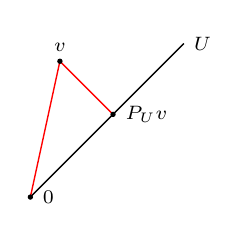
\begin{tikzpicture}[scale=.75]
  \draw[line width=.5pt] (0,0)--(2.6,2.6) node[right,font=\scriptsize] {$U$};
  \draw[red,line width=.5pt] (0,0)--(.5,2.3)--(1.4,1.4);
  \fill (0,0) circle (1.3pt) node[right=1pt,font=\scriptsize] {$0$};
  \fill (.5,2.3) circle (1.3pt) node[above,font=\scriptsize] {$v$};
  \fill (1.4,1.4) circle (1.3pt) node[right=1pt,font=\scriptsize] {$P_Uv$};
\end{tikzpicture}}{$P_Uv$ is the closest point in $U$ to $v$.}%
where the first line above holds because $0\le\norm{P_Uv-u}^2$, the second line
above comes from the Pythagorean theorem [which applies because
$v-P_Uv\in U^\perp$ by \ref{ax:6.57}(f), and $P_Uv-u\in U$], and the third line
above holds by simple algebra. Taking square roots gives the desired
inequality.

The inequality proved above is an equality if and only if \ref{ax:6.62} is an
equality, which happens if and only if $\norm{P_Uv-u}=0$, which happens if and
only if $u=P_Uv$.
\end{proof}

The last result is often combined with the formula \ref{ax:6.57}(i) to compute
explicit solutions to minimization problems, as in the following example.

\begin{example}[Using linear algebra to approximate the sine
function]\label{ax:6.63}
Suppose we want to find a polynomial $u$ with real coefficients and of degree
at most $5$ that approximates the sine function as well as possible on the
interval $[-\pi,\pi]$, in the sense that
\[ \int_{-\pi}^{\pi} \abs{\sin x-u(x)}^2\,dx \]
is as small as possible.

Let $C[-\pi,\pi]$ denote the real inner product space of continuous real-valued
functions on $[-\pi,\pi]$ with inner product\axeqstep{ax:6.64}
\begin{equation*}
\ip{f}{g} = \int_{-\pi}^{\pi} fg. \axeqtag
\end{equation*}
Let $v\in C[-\pi,\pi]$ be the function defined by $v(x)=\sin x$. Let $U$ denote
the subspace of $C[-\pi,\pi]$ consisting of the polynomials with real
coefficients and of degree at most $5$. Our problem can now be reformulated as
follows:
\[ \text{Find } u\in U \text{ such that } \norm{v-u}
   \text{ is as small as possible.} \]

To compute the solution to our approximation problem, first apply the
Gram--Schmidt procedure (using the inner product given by \ref{ax:6.64}) to the
basis $1,x,x^2,x^3,x^4,x^5$ of $U$, producing an orthonormal basis
$e_1,e_2,e_3,e_4,e_5,e_6$ of $U$. Then, again using the inner product given by
\ref{ax:6.64}, compute $P_Uv$ using \ref{ax:6.57}(i) (with $m=6$). Doing this
computation shows that $P_Uv$ is the function $u$ defined
by\axeqstep{ax:6.65}
\begin{equation*}
u(x) = 0.987862x-0.155271x^3+0.00564312x^5, \axeqtag
\end{equation*}
where the $\pi$'s that appear in the exact answer have been replaced with a
good decimal approximation. By \ref{ax:6.61}, the polynomial $u$ above is the
best approximation to the sine function on $[-\pi,\pi]$ using polynomials of
degree at most $5$ (here ``best approximation'' means in the sense of
minimizing $\int_{-\pi}^{\pi}\abs{\sin x-u(x)}^2\,dx$).

To see how good this approximation is, the next figure shows the graphs of both
the sine function and our approximation $u$ given by \ref{ax:6.65} over the
interval $[-\pi,\pi]$.
\begin{center}
\begin{tikzpicture}[xscale=1.2,yscale=1]
  \draw[line width=.4pt] (-3.3,0)--(3.3,0);
  \draw[line width=.4pt] (0,-1.15)--(0,1.15);
  \foreach \y in {-1,1} \draw (0,\y)--(-.06,\y) node[left,font=\scriptsize]
    {$\y$};
  \foreach \x/\l in {-pi/-\pi,pi/\pi} \draw (\x,0)--(\x,-.06)
    node[below,font=\scriptsize] {$\l$};
  \draw[blue,line width=.6pt,domain=-pi:pi,samples=120]
    plot (\x,{0.987862*\x-0.155271*\x^3+0.00564312*\x^5});
  \draw[red,line width=.6pt,domain=-pi:pi,samples=120] plot (\x,{sin(\x r)});
\end{tikzpicture}
\captionof*{figure}{Graphs on $[-\pi,\pi]$ of the sine function (red) and its
best fifth degree polynomial approximation $u$ (blue) from \ref{ax:6.65}.}
\end{center}

Our approximation \ref{ax:6.65} is so accurate that the two graphs are almost
identical---our eyes may see only one graph! Here the red graph is placed
almost exactly over the blue graph. If you are viewing this on an electronic
device, enlarge the picture above by 400\% near $\pi$ or $-\pi$ to see a small
gap between the two graphs.

Another well-known approximation to the sine function by a polynomial of degree
$5$ is given by the Taylor polynomial $p$ defined by\axeqstep{ax:6.66}
\begin{equation*}
p(x) = x-\frac{x^3}{3!}+\frac{x^5}{5!}. \axeqtag
\end{equation*}
To see how good this approximation is, the next picture shows the graphs of
both the sine function and the Taylor polynomial $p$ over the interval
$[-\pi,\pi]$.
\begin{center}
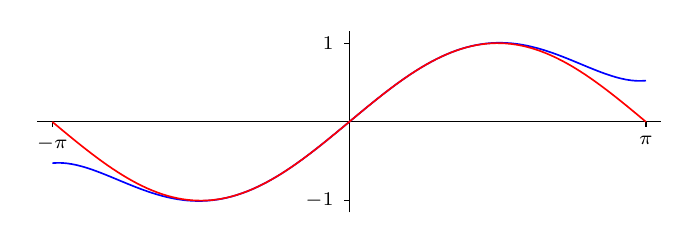
\begin{tikzpicture}[xscale=1.2,yscale=1]
  \draw[line width=.4pt] (-3.3,0)--(3.3,0);
  \draw[line width=.4pt] (0,-1.15)--(0,1.15);
  \foreach \y in {-1,1} \draw (0,\y)--(-.06,\y) node[left,font=\scriptsize]
    {$\y$};
  \foreach \x/\l in {-pi/-\pi,pi/\pi} \draw (\x,0)--(\x,-.06)
    node[below,font=\scriptsize] {$\l$};
  \draw[blue,line width=.6pt,domain=-pi:pi,samples=120]
    plot (\x,{\x-\x^3/6+\x^5/120});
  \draw[red,line width=.6pt,domain=-pi:pi,samples=120] plot (\x,{sin(\x r)});
\end{tikzpicture}
\captionof*{figure}{Graphs on $[-\pi,\pi]$ of the sine function (red) and the
Taylor polynomial (blue) from \ref{ax:6.66}.}
\end{center}

The Taylor polynomial of degree $5$ is an excellent approximation to $\sin x$
for $x$ near $0$. But the picture above shows that for $\abs{x}>2$, the Taylor
polynomial is not so accurate, especially compared to \ref{ax:6.65}. For
example, taking $x=3$, our approximation \ref{ax:6.65} estimates $\sin 3$ with
an error of approximately $0.001$, but the Taylor polynomial \ref{ax:6.66}
estimates $\sin 3$ with an error of approximately $0.4$. Thus at $x=3$, the
error in the Taylor polynomial is hundreds of times larger than the error given
by \ref{ax:6.65}. Linear algebra has helped us discover an approximation to the
sine function that improves upon what we learned in calculus!
\end{example}

\subsection{Pseudoinverse}

Suppose $T\in\Lin(V,W)$ and $w\in W$. Consider the problem of finding $v\in V$
such that
\[ Tv = w. \]
For example, if $V=\F^n$ and $W=\F^m$, then the equation above could represent
a system of $m$ linear equations in $n$ unknowns $v_1,\dots,v_n$, where
$v=(v_1,\dots,v_n)$.

If $T$ is invertible, then the unique solution to the equation above is
$v=T^{-1}w$. However, if $T$ is not invertible, then for some $w\in W$ there
may not exist any solutions of the equation above, and for some $w\in W$ there
may exist infinitely many solutions of the equation above.

If $T$ is not invertible, then we can still try to do as well as possible with
the equation above. For example, if the equation above has no solutions, then
instead of solving the equation $Tv-w=0$, we can try to find $v\in V$ such that
$\norm{Tv-w}$ is as small as possible. As another example, if the equation
above has infinitely many solutions $v\in V$, then among all those solutions we
can try to find one such that $\norm{v}$ is as small as possible.

The pseudoinverse will provide the tool to solve the equation above as well as
possible, even when $T$ is not invertible. We need the next result to define
the pseudoinverse.

In the next two proofs, we will use without further comment the result that if
$V$ is finite-dimensional and $T\in\Lin(V,W)$, then $\nul T$,
$(\nul T)^\perp$, and $\range T$ are all finite-dimensional.

\begin{result}[Restriction of a linear map to obtain a one-to-one and onto
map]\label{ax:6.67}
Suppose $V$ is finite-dimensional and $T\in\Lin(V,W)$. Then
$T|_{(\nul T)^\perp}$ is an injective map of $(\nul T)^\perp$ onto $\range T$.
\end{result}

\begin{proof}
Suppose that $v\in(\nul T)^\perp$ and $T|_{(\nul T)^\perp}v=0$. Hence $Tv=0$
and thus $v\in(\nul T)\cap(\nul T)^\perp$, which implies that $v=0$ [by
\ref{ax:6.48}(d)]. Hence $\nul\bigl(T|_{(\nul T)^\perp}\bigr)=\{0\}$, which
implies that $T|_{(\nul T)^\perp}$ is injective, as desired.

Clearly $\range\bigl(T|_{(\nul T)^\perp}\bigr)\subseteq\range T$. To prove the
inclusion in the other direction, suppose $w\in\range T$. Hence there exists
$v\in V$ such that $w=Tv$. There exist $u\in\nul T$ and $x\in(\nul T)^\perp$
such that $v=u+x$ (by \ref{ax:6.49}). Now
\[ T|_{(\nul T)^\perp}x = Tx = Tv-Tu = w-0 = w, \]
which shows that $w\in\range T|_{(\nul T)^\perp}$. Hence
$\range T\subseteq\range T|_{(\nul T)^\perp}$, completing the proof that
$\range T|_{(\nul T)^\perp}=\range T$.
\end{proof}

\marginnote{To produce the pseudoinverse notation $T^\dagger$ in \TeX, type
\texttt{T\textasciicircum\textbackslash dagger}.}%
Now we can define the pseudoinverse $T^\dagger$ (pronounced ``$T$ dagger'') of
a linear map $T$. In the next definition (and from now on), think of
$T|_{(\nul T)^\perp}$ as an invertible linear map from $(\nul T)^\perp$ onto
$\range T$, as is justified by the result above.

\begin{definition}[Pseudoinverse, $T^\dagger$]\label{ax:6.68}
Suppose that $V$ is finite-dimensional and $T\in\Lin(V,W)$. The
\emph{pseudoinverse} $T^\dagger\in\Lin(W,V)$ of $T$ is the linear map from $W$
to $V$ defined by
\[ T^\dagger w = \bigl(T|_{(\nul T)^\perp}\bigr)^{-1}P_{\range T}w \]
for each $w\in W$.
\end{definition}

Recall that $P_{\range T}w=0$ if $w\in(\range T)^\perp$ and
$P_{\range T}w=w$ if $w\in\range T$. Thus if $w\in(\range T)^\perp$, then
$T^\dagger w=0$, and if $w\in\range T$, then $T^\dagger w$ is the unique
element of $(\nul T)^\perp$ such that $T(T^\dagger w)=w$.

The pseudoinverse behaves much like an inverse, as we will see.

\begin{result}[Algebraic properties of the pseudoinverse]\label{ax:6.69}
Suppose $V$ is finite-dimensional and $T\in\Lin(V,W)$.
\begin{parts}
\item If $T$ is invertible, then $T^\dagger=T^{-1}$.
\item $TT^\dagger=P_{\range T}=$ the orthogonal projection of $W$ onto
  $\range T$.
\item $T^\dagger T=P_{(\nul T)^\perp}=$ the orthogonal projection of $V$ onto
  $(\nul T)^\perp$.
\end{parts}
\end{result}

\begin{proof}\leavevmode
\begin{parts}
\item Suppose $T$ is invertible. Then $(\nul T)^\perp=V$ and $\range T=W$.
  Thus $T|_{(\nul T)^\perp}=T$ and $P_{\range T}$ is the identity operator on
  $W$. Hence $T^\dagger=T^{-1}$.
\item Suppose $w\in\range T$. Thus
  \[ TT^\dagger w = T\bigl(T|_{(\nul T)^\perp}\bigr)^{-1}w = w
     = P_{\range T}w. \]
  If $w\in(\range T)^\perp$, then $T^\dagger w=0$. Hence
  $TT^\dagger w=0=P_{\range T}w$. Thus $TT^\dagger$ and $P_{\range T}$ agree on
  $\range T$ and on $(\range T)^\perp$. Hence these two linear maps are equal
  (by \ref{ax:6.49}).
\item Suppose $v\in(\nul T)^\perp$. Because $Tv\in\range T$, the definition of
  $T^\dagger$ shows that
  \[ T^\dagger(Tv) = \bigl(T|_{(\nul T)^\perp}\bigr)^{-1}(Tv) = v
     = P_{(\nul T)^\perp}v. \]
  If $v\in\nul T$, then $T^\dagger Tv=0=P_{(\nul T)^\perp}v$. Thus
  $T^\dagger T$ and $P_{(\nul T)^\perp}$ agree on $(\nul T)^\perp$ and on
  $\nul T$. Hence these two linear maps are equal (by \ref{ax:6.49}).
  \qedhere
\end{parts}
\end{proof}

\marginnote{The pseudoinverse is also called the Moore--Penrose inverse.}%
Suppose that $T\in\Lin(V,W)$. If $T$ is surjective, then $TT^\dagger$ is the
identity operator on $W$, as follows from (b) in the result above. If $T$ is
injective, then $T^\dagger T$ is the identity operator on $V$, as follows from
(c) in the result above. For additional algebraic properties of the
pseudoinverse, see Exercises 19--23.

For $T\in\Lin(V,W)$ and $w\in W$, we now return to the problem of finding
$v\in V$ that solves the equation
\[ Tv = w. \]
As we noted earlier, if $T$ is invertible, then $v=T^{-1}w$ is the unique
solution, but if $T$ is not invertible, then $T^{-1}$ is not defined. However,
the pseudoinverse $T^\dagger$ is defined. Taking $v=T^\dagger w$ makes $Tv$ as
close to $w$ as possible, as shown by (a) of the next result. Thus the
pseudoinverse provides what is called a \emph{best fit} to the equation above.

Among all vectors $v\in V$ that make $Tv$ as close as possible to $w$, the
vector $T^\dagger w$ has the smallest norm, as shown by combining (b) in the
next result with the condition for equality in (a).

\begin{result}[Pseudoinverse provides best approximate solution or best
solution]\label{ax:6.70}
Suppose $V$ is finite-dimensional, $T\in\Lin(V,W)$, and $w\in W$.
\begin{parts}
\item If $v\in V$, then
  \[ \bigl\lVert T(T^\dagger w)-w\bigr\rVert \le \norm{Tv-w}, \]
  with equality if and only if $v\in T^\dagger w+\nul T$.
\item If $v\in T^\dagger w+\nul T$, then
  \[ \bigl\lVert T^\dagger w\bigr\rVert \le \norm{v}, \]
  with equality if and only if $v=T^\dagger w$.
\end{parts}
\end{result}

\begin{proof}\leavevmode
\begin{parts}
\item Suppose $v\in V$. Then
  \[ Tv-w = (Tv-TT^\dagger w)+(TT^\dagger w-w). \]
  The first term in parentheses above is in $\range T$. Because the operator
  $TT^\dagger$ is the orthogonal projection of $W$ onto $\range T$ [by
  \ref{ax:6.69}(b)], the second term in parentheses above is in
  $(\range T)^\perp$ [see \ref{ax:6.57}(f)].

  Thus the Pythagorean theorem implies the desired inequality that the norm of
  the second term in parentheses above is less than or equal to
  $\norm{Tv-w}$, with equality if and only if the first term in parentheses
  above equals $0$. Hence we have equality if and only if
  $v-T^\dagger w\in\nul T$, which is equivalent to the statement that
  $v\in T^\dagger w+\nul T$, completing the proof of (a).
\item Suppose $v\in T^\dagger w+\nul T$. Hence $v-T^\dagger w\in\nul T$. Now
  \[ v = (v-T^\dagger w)+T^\dagger w. \]
  The definition of $T^\dagger$ implies that $T^\dagger w\in(\nul T)^\perp$.
  Thus the Pythagorean theorem implies that
  $\bigl\lVert T^\dagger w\bigr\rVert\le\norm{v}$, with equality if and only
  if $v=T^\dagger w$. \qedhere
\end{parts}
\end{proof}

A formula for $T^\dagger$ will be given in the next chapter (see
\ref{ax:7.78}).

\begin{example}[Pseudoinverse of a linear map from $\F^4$ to
$\F^3$]\label{ax:6.71}
Suppose $T\in\Lin(\F^4,\F^3)$ is defined by
\[ T(a,b,c,d) = (a+b+c,\,2c+d,\,0). \]
This linear map is neither injective nor surjective, but we can compute its
pseudoinverse. To do this, first note that
$\range T=\{(x,y,0) : x,y\in\F\}$. Thus
\[ P_{\range T}(x,y,z) = (x,y,0) \]
for each $(x,y,z)\in\F^3$. Also,
\[ \nul T = \{(a,b,c,d)\in\F^4 : a+b+c=0 \text{ and } 2c+d=0\}. \]
The list $(-1,1,0,0)$, $(-1,0,1,-2)$ of two vectors in $\nul T$ spans $\nul T$
because if $(a,b,c,d)\in\nul T$ then
\[ (a,b,c,d) = b(-1,1,0,0)+c(-1,0,1,-2). \]
Because the list $(-1,1,0,0)$, $(-1,0,1,-2)$ is linearly independent, this list
is a basis of $\nul T$.

Now suppose $(x,y,z)\in\F^3$. Then\axeqstep{ax:6.72}
\begin{equation*}
T^\dagger(x,y,z) = \bigl(T|_{(\nul T)^\perp}\bigr)^{-1}P_{\range T}(x,y,z)
  = \bigl(T|_{(\nul T)^\perp}\bigr)^{-1}(x,y,0). \axeqtag
\end{equation*}
The right side of the equation above is the vector $(a,b,c,d)\in\F^4$ such that
$T(a,b,c,d)=(x,y,0)$ and $(a,b,c,d)\in(\nul T)^\perp$. In other words,
$a,b,c,d$ must satisfy the following equations:
\begin{align*}
a+b+c &= x\\
2c+d &= y\\
-a+b &= 0\\
-a+c-2d &= 0,
\end{align*}
where the first two equations are equivalent to the equation
$T(a,b,c,d)=(x,y,0)$ and the last two equations come from the condition for
$(a,b,c,d)$ to be orthogonal to each of the basis vectors $(-1,1,0,0)$,
$(-1,0,1,-2)$ in this basis of $\nul T$. Thinking of $x$ and $y$ as constants
and $a$, $b$, $c$, $d$ as unknowns, we can solve the system above of four
equations in four unknowns, getting
\[ a=(1/11)(5x-2y),\ b=(1/11)(5x-2y),\
   c=(1/11)(x+4y),\ d=(1/11)(-2x+3y). \]
Hence \ref{ax:6.72} tells us that
\[ T^\dagger(x,y,z) = (1/11)(5x-2y,\,5x-2y,\,x+4y,\,-2x+3y). \]
The formula above for $T^\dagger$ shows that $TT^\dagger(x,y,z)=(x,y,0)$ for
all $(x,y,z)\in\F^3$, which illustrates the equation $TT^\dagger=P_{\range T}$
from \ref{ax:6.69}(b).
\end{example}

% ------------------------------------------------------------------ exercises
\exercisesheading{6C}

\begin{exercise}
Suppose $v_1,\dots,v_m\in V$. Prove that
\[ \{v_1,\dots,v_m\}^\perp = \bigl(\spn(v_1,\dots,v_m)\bigr)^\perp. \]
\end{exercise}

\begin{exercise}
Suppose $U$ is a subspace of $V$ with basis $u_1,\dots,u_m$ and
\[ u_1,\dots,u_m,v_1,\dots,v_n \]
is a basis of $V$. Prove that if the Gram--Schmidt procedure is applied to the
basis of $V$ above, producing a list $e_1,\dots,e_m,f_1,\dots,f_n$, then
$e_1,\dots,e_m$ is an orthonormal basis of $U$ and $f_1,\dots,f_n$ is an
orthonormal basis of $U^\perp$.
\end{exercise}

\begin{exercise}
Suppose $U$ is the subspace of $\R^4$ defined by
\[ U = \spn\bigl((1,2,3,-4),(-5,4,3,2)\bigr). \]
Find an orthonormal basis of $U$ and an orthonormal basis of $U^\perp$.
\end{exercise}

\begin{exercise}
Suppose $e_1,\dots,e_n$ is a list of vectors in $V$ with $\norm{e_k}=1$ for each
$k=1,\dots,n$ and
\[ \norm{v}^2 = \abs{\ip{v}{e_1}}^2+\cdots+\abs{\ip{v}{e_n}}^2 \]
for all $v\in V$. Prove that $e_1,\dots,e_n$ is an orthonormal basis of $V$.
\exnote{This exercise provides a converse to \ref{ax:6.30}(b).}
\end{exercise}

\begin{exercise}
Suppose that $V$ is finite-dimensional and $U$ is a subspace of $V$. Show that
$P_{U^\perp}=I-P_U$, where $I$ is the identity operator on $V$.
\end{exercise}

\begin{exercise}
Suppose $V$ is finite-dimensional and $T\in\Lin(V,W)$. Show that
\[ T = TP_{(\nul T)^\perp} = P_{\range T}T. \]
\end{exercise}

\begin{exercise}
Suppose that $X$ and $Y$ are finite-dimensional subspaces of $V$. Prove that
$P_XP_Y=0$ if and only if $\ip{x}{y}=0$ for all $x\in X$ and all $y\in Y$.
\end{exercise}

\begin{exercise}
Suppose $U$ is a finite-dimensional subspace of $V$ and $v\in V$. Define a
linear functional $\varphi\colon U\to\F$ by
\[ \varphi(u) = \ip{u}{v} \]
for all $u\in U$. By the Riesz representation theorem (\ref{ax:6.42}) as
applied to the inner product space $U$, there exists a unique vector $w\in U$
such that
\[ \varphi(u) = \ip{u}{w} \]
for all $u\in U$. Show that $w=P_Uv$.
\end{exercise}

\begin{exercise}
Suppose $V$ is finite-dimensional. Suppose $P\in\Lin(V)$ is such that $P^2=P$
and every vector in $\nul P$ is orthogonal to every vector in $\range P$. Prove
that there exists a subspace $U$ of $V$ such that $P=P_U$.
\end{exercise}

\begin{exercise}
Suppose $V$ is finite-dimensional and $P\in\Lin(V)$ is such that $P^2=P$ and
\[ \norm{Pv} \le \norm{v} \]
for every $v\in V$. Prove that there exists a subspace $U$ of $V$ such that
$P=P_U$.
\end{exercise}

\begin{exercise}
Suppose $T\in\Lin(V)$ and $U$ is a finite-dimensional subspace of $V$. Prove
that
\[ U \text{ is invariant under } T \iff P_UTP_U=TP_U. \]
\end{exercise}

\begin{exercise}
Suppose $V$ is finite-dimensional, $T\in\Lin(V)$, and $U$ is a subspace of $V$.
Prove that
\[ U \text{ and } U^\perp \text{ are both invariant under } T
   \iff P_UT=TP_U. \]
\end{exercise}

\begin{exercise}
Suppose $\F=\R$ and $V$ is finite-dimensional. For each $v\in V$, let
$\varphi_v$ denote the linear functional on $V$ defined by
\[ \varphi_v(u) = \ip{u}{v} \]
for all $u\in V$.
\begin{parts}
\item Show that $v\mapsto\varphi_v$ is an injective linear map from $V$ to
  $V'$.
\item Use (a) and a dimension-counting argument to show that
  $v\mapsto\varphi_v$ is an isomorphism from $V$ onto $V'$.
\end{parts}
\exnote{The purpose of this exercise is to give an alternative proof of the
Riesz representation theorem (\ref{ax:6.42} and \ref{ax:6.58}) when $\F=\R$.
Thus you should not use the Riesz representation theorem as a tool in your
solution.}
\end{exercise}

\begin{exercise}
Suppose that $e_1,\dots,e_n$ is an orthonormal basis of $V$. Explain why the
dual basis (see \ref{ax:3.112}) of $e_1,\dots,e_n$ is $e_1,\dots,e_n$ under the
identification of $V'$ with $V$ provided by the Riesz representation theorem
(\ref{ax:6.58}).
\end{exercise}

\begin{exercise}
In $\R^4$, let
\[ U = \spn\bigl((1,1,0,0),(1,1,1,2)\bigr). \]
Find $u\in U$ such that $\norm{u-(1,2,3,4)}$ is as small as possible.
\end{exercise}

\begin{exercise}
Suppose $C[-1,1]$ is the vector space of continuous real-valued functions on
the interval $[-1,1]$ with inner product given by
\[ \ip{f}{g} = \int_{-1}^{1} fg \]
for all $f,g\in C[-1,1]$. Let $U$ be the subspace of $C[-1,1]$ defined by
\[ U = \{f\in C[-1,1] : f(0)=0\}. \]
\begin{parts}
\item Show that $U^\perp=\{0\}$.
\item Show that \ref{ax:6.49} and \ref{ax:6.52} do not hold without the
  finite-dimensional hypothesis.
\end{parts}
\end{exercise}

\begin{exercise}
Find $p\in\Poly_3(\R)$ such that $p(0)=0$, $p'(0)=0$, and
$\int_0^1\abs{2+3x-p(x)}^2\,dx$ is as small as possible.
\end{exercise}

\begin{exercise}
Find $p\in\Poly_5(\R)$ that makes $\int_{-\pi}^{\pi}\abs{\sin x-p(x)}^2\,dx$ as
small as possible.
\exnote{The polynomial \ref{ax:6.65} is an excellent approximation to the
answer to this exercise, but here you are asked to find the exact solution,
which involves powers of $\pi$. A computer that can perform symbolic
integration should help.}
\end{exercise}

\begin{exercise}
Suppose $V$ is finite-dimensional and $P\in\Lin(V)$ is an orthogonal projection
of $V$ onto some subspace of $V$. Prove that $P^\dagger=P$.
\end{exercise}

\begin{exercise}
Suppose $V$ is finite-dimensional and $T\in\Lin(V,W)$. Show that
\[ \nul T^\dagger = (\range T)^\perp \quad\text{and}\quad
   \range T^\dagger = (\nul T)^\perp. \]
\end{exercise}

\begin{exercise}
Suppose $T\in\Lin(\F^3,\F^2)$ is defined by
\[ T(a,b,c) = (a+b+c,\,2b+3c). \]
\begin{parts}
\item For $(x,y)\in\F^2$, find a formula for $T^\dagger(x,y)$.
\item Verify that the equation $TT^\dagger=P_{\range T}$ from
  \ref{ax:6.69}(b) holds with the formula for $T^\dagger$ obtained in (a).
\item Verify that the equation $T^\dagger T=P_{(\nul T)^\perp}$ from
  \ref{ax:6.69}(c) holds with the formula for $T^\dagger$ obtained in (a).
\end{parts}
\end{exercise}

\begin{exercise}
Suppose $V$ is finite-dimensional and $T\in\Lin(V,W)$. Prove that
\[ TT^\dagger T = T \quad\text{and}\quad T^\dagger TT^\dagger = T^\dagger. \]
\exnote{Both formulas above clearly hold if $T$ is invertible because in that
case we can replace $T^\dagger$ with $T^{-1}$.}
\end{exercise}

\begin{exercise}
Suppose $V$ and $W$ are finite-dimensional and $T\in\Lin(V,W)$. Prove that
\[ (T^\dagger)^\dagger = T. \]
\exnote{The equation above is analogous to the equation $(T^{-1})^{-1}=T$ that
holds if $T$ is invertible.}
\end{exercise}


% Chapter 7: assembled from chapters/ch07/*.tex
% Source: book p. 227 (PDF 241).
\chapter{Operators on Inner Product Spaces}

The deepest results related to inner product spaces deal with the subject to
which we now turn---linear maps and operators on inner product spaces. As we
will see, good theorems can be proved by exploiting properties of the adjoint.

The hugely important spectral theorem will provide a complete description of
self-adjoint operators on real inner product spaces and of normal operators on
complex inner product spaces. We will then use the spectral theorem to help
understand positive operators and unitary operators, which will lead to unitary
matrices and matrix factorizations. The spectral theorem will also lead to the
popular singular value decomposition, which will lead to the polar
decomposition.

The most important results in the rest of this book are valid only in finite
dimensions. Thus from now on we assume that $V$ and $W$ are finite-dimensional.

\begin{definition*}[Standing assumptions for this chapter]\leavevmode
\begin{itemize}
\item $\F$ denotes $\R$ or $\C$.
\item $V$ and $W$ are nonzero finite-dimensional inner product spaces over $\F$.
\end{itemize}
\end{definition*}

% Source: book pp. 228--242 (PDF 242--256). No solutions in the manual.
% a numbered display (Axler numbers a few equations with the item counter):
%   text\axeqstep{ax:7.15}  \[ ... \tag{\thetheorem} \]
\DeclareRobustCommand\axeqstep[1]{\refstepcounter{theorem}\label{#1}}
% the small italic comment that follows some exercises
\section{Self-Adjoint and Normal Operators}

\subsection{Adjoints}

\begin{definition}[Adjoint, $T^*$]\label{ax:7.1}
Suppose $T\in\Lin(V,W)$. The \emph{adjoint} of $T$ is the function
$T^*\colon W\to V$ such that
\[ \ip{Tv}{w} = \ip{v}{T^*w} \]
for every $v\in V$ and every $w\in W$.
\end{definition}

\marginnote{The word \textbf{adjoint} has another meaning in linear algebra. In
case you encounter the second meaning elsewhere, be warned that the two meanings
for adjoint are unrelated to each other.}%
To see why the definition above makes sense, suppose $T\in\Lin(V,W)$. Fix
$w\in W$. Consider the linear functional
\[ v\mapsto\ip{Tv}{w} \]
on $V$ that maps $v\in V$ to $\ip{Tv}{w}$; this linear functional depends on $T$
and $w$. By the Riesz representation theorem (\ref{ax:6.42}), there exists a
unique vector in $V$ such that this linear functional is given by taking the
inner product with it. We call this unique vector $T^*w$. In other words, $T^*w$
is the unique vector in $V$ such that
\[ \ip{Tv}{w} = \ip{v}{T^*w} \]
for every $v\in V$.

In the equation above, the inner product on the left takes place in $W$ and the
inner product on the right takes place in $V$. However, we use the same
notation $\ip{\cdot}{\cdot}$ for both inner products.

\begin{example}[Adjoint of a linear map from $\R^3$ to $\R^2$]\label{ax:7.2}
Define $T\colon\R^3\to\R^2$ by
\[ T(x_1,x_2,x_3) = (x_2+3x_3,\,2x_1). \]
To compute $T^*$, suppose $(x_1,x_2,x_3)\in\R^3$ and $(y_1,y_2)\in\R^2$. Then
\begin{align*}
\bigl\langle T(x_1,x_2,x_3),(y_1,y_2)\bigr\rangle
  &= \bigl\langle (x_2+3x_3,\,2x_1),(y_1,y_2)\bigr\rangle\\
  &= x_2y_1+3x_3y_1+2x_1y_2\\
  &= \bigl\langle (x_1,x_2,x_3),(2y_2,y_1,3y_1)\bigr\rangle.
\end{align*}
The equation above and the definition of the adjoint imply that
\[ T^*(y_1,y_2) = (2y_2,y_1,3y_1). \]
\end{example}

\begin{example}[Adjoint of a linear map with range of dimension at most $1$]%
\label{ax:7.3}
Fix $u\in V$ and $x\in W$. Define $T\in\Lin(V,W)$ by
\[ Tv = \ip{v}{u}x \]
for each $v\in V$. To compute $T^*$, suppose $v\in V$ and $w\in W$. Then
\begin{align*}
\ip{Tv}{w} &= \bigl\langle \ip{v}{u}x,w\bigr\rangle\\
           &= \ip{v}{u}\ip{x}{w}\\
           &= \bigl\langle v,\ip{w}{x}u\bigr\rangle.
\end{align*}
Thus
\[ T^*w = \ip{w}{x}u. \]
\end{example}

\marginnote[-3em]{The two examples above and the proof below use a common technique
for computing $T^*$: start with a formula for $\ip{Tv}{w}$ then manipulate it to
get just $v$ in the first slot; the entry in the second slot will then be
$T^*w$.}%
In the two examples above, $T^*$ turned out to be not just a function from $W$
to $V$ but a linear map from $W$ to $V$. This behavior is true in general, as
shown by the next result.

\begin{result}[Adjoint of a linear map is a linear map]\label{ax:7.4}
If $T\in\Lin(V,W)$, then $T^*\in\Lin(W,V)$.
\end{result}

\begin{proof}
Suppose $T\in\Lin(V,W)$. If $v\in V$ and $w_1,w_2\in W$, then
\begin{align*}
\ip{Tv}{w_1+w_2} &= \ip{Tv}{w_1}+\ip{Tv}{w_2}\\
                 &= \ip{v}{T^*w_1}+\ip{v}{T^*w_2}\\
                 &= \ip{v}{T^*w_1+T^*w_2}.
\end{align*}
The equation above shows that
\[ T^*(w_1+w_2) = T^*w_1+T^*w_2. \]

If $v\in V$, $\lambda\in\F$, and $w\in W$, then
\begin{align*}
\ip{Tv}{\lambda w} &= \overline{\lambda}\ip{Tv}{w}\\
                   &= \overline{\lambda}\ip{v}{T^*w}\\
                   &= \ip{v}{\lambda T^*w}.
\end{align*}
The equation above shows that
\[ T^*(\lambda w) = \lambda T^*w. \]

Thus $T^*$ is a linear map, as desired.
\end{proof}

\begin{result}[Properties of the adjoint]\label{ax:7.5}
Suppose $T\in\Lin(V,W)$. Then
\begin{parts}
\item $(S+T)^*=S^*+T^*$ for all $S\in\Lin(V,W)$;
\item $(\lambda T)^*=\overline{\lambda}T^*$ for all $\lambda\in\F$;
\item $(T^*)^*=T$;
\item $(ST)^*=T^*S^*$ for all $S\in\Lin(W,U)$ (here $U$ is a finite-dimensional
  inner product space over $\F$);
\item $I^*=I$, where $I$ is the identity operator on $V$;
\item if $T$ is invertible, then $T^*$ is invertible and
  $(T^*)^{-1}=(T^{-1})^*$.
\end{parts}
\end{result}

\begin{proof}
Suppose $v\in V$ and $w\in W$.
\begin{parts}
\item If $S\in\Lin(V,W)$, then
  \begin{align*}
  \bigl\langle (S+T)v,w\bigr\rangle &= \ip{Sv}{w}+\ip{Tv}{w}\\
    &= \ip{v}{S^*w}+\ip{v}{T^*w}\\
    &= \ip{v}{S^*w+T^*w}.
  \end{align*}
  Thus $(S+T)^*w=S^*w+T^*w$, as desired.
\item If $\lambda\in\F$, then
  \[ \bigl\langle (\lambda T)v,w\bigr\rangle = \lambda\ip{Tv}{w}
     = \lambda\ip{v}{T^*w} = \ip{v}{\overline{\lambda}T^*w}. \]
  Thus $(\lambda T)^*w=\overline{\lambda}T^*w$, as desired.
\item We have
  \[ \ip{T^*w}{v} = \overline{\ip{v}{T^*w}} = \overline{\ip{Tv}{w}}
     = \ip{w}{Tv}. \]
  Thus $(T^*)^*v=Tv$, as desired.
\item Suppose $S\in\Lin(W,U)$ and $u\in U$. Then
  \[ \bigl\langle (ST)v,u\bigr\rangle = \bigl\langle S(Tv),u\bigr\rangle
     = \ip{Tv}{S^*u} = \bigl\langle v,T^*(S^*u)\bigr\rangle. \]
  Thus $(ST)^*u=T^*(S^*u)$, as desired.
\item Suppose $u\in V$. Then
  \[ \ip{Iu}{v} = \ip{u}{v}. \]
  Thus $I^*v=v$, as desired.
\item Suppose $T$ is invertible. Take adjoints of both sides of the equation
  $T^{-1}T=I$, then use (d) and (e) to show that $T^*(T^{-1})^*=I$. Similarly,
  the equation $TT^{-1}=I$ implies $(T^{-1})^*T^*=I$. Thus $(T^{-1})^*$ is the
  inverse of $T^*$, as desired. \qedhere
\end{parts}
\end{proof}

If $\F=\R$, then the map $T\mapsto T^*$ is a linear map from $\Lin(V,W)$ to
$\Lin(W,V)$, as follows from (a) and (b) of the result above. However, if
$\F=\C$, then this map is not linear because of the complex conjugate that
appears in (b).

The next result shows the relationship between the null space and the range of
a linear map and its adjoint.

\begin{result}[Null space and range of $T^*$]\label{ax:7.6}
Suppose $T\in\Lin(V,W)$. Then
\begin{parts}
\item $\nul T^*=(\range T)^\perp$;
\item $\range T^*=(\nul T)^\perp$;
\item $\nul T=(\range T^*)^\perp$;
\item $\range T=(\nul T^*)^\perp$.
\end{parts}
\end{result}

\begin{proof}
We begin by proving (a). Let $w\in W$. Then
\begin{align*}
w\in\nul T^* &\iff T^*w=0\\
  &\iff \ip{v}{T^*w}=0 \text{ for all } v\in V\\
  &\iff \ip{Tv}{w}=0 \text{ for all } v\in V\\
  &\iff w\in(\range T)^\perp.
\end{align*}
Thus $\nul T^*=(\range T)^\perp$, proving (a).

If we take the orthogonal complement of both sides of (a), we get (d), where we
have used \ref{ax:6.52}. Replacing $T$ with $T^*$ in (a) gives (c), where we
have used \ref{ax:7.5}(c). Finally, replacing $T$ with $T^*$ in (d) gives (b).
\end{proof}

As we will soon see, the next definition is intimately connected to the matrix
of the adjoint of a linear map.

\begin{definition}[Conjugate transpose, $A^*$]\label{ax:7.7}
The \emph{conjugate transpose} of an $m$-by-$n$ matrix $A$ is the $n$-by-$m$
matrix $A^*$ obtained by interchanging the rows and columns and then taking the
complex conjugate of each entry. In other words, if $j\in\{1,\dots,n\}$ and
$k\in\{1,\dots,m\}$, then
\[ (A^*)_{j,k} = \overline{A_{k,j}}. \]
\end{definition}

\begin{example}[Conjugate transpose of a $2$-by-$3$ matrix]\label{ax:7.8}
The conjugate transpose of the $2$-by-$3$ matrix
$\begin{pmatrix} 2 & 3+4i & 7\\ 6 & 5 & 8i \end{pmatrix}$
is the $3$-by-$2$ matrix
\[ \begin{pmatrix} 2 & 6\\ 3-4i & 5\\ 7 & -8i \end{pmatrix}. \]
\end{example}

% the first note sits beside Example 7.8 (a note cannot go inside the box)
\marginnote[-24mm]{If a matrix $A$ has only real entries, then $A^*=A^{\mathrm{t}}$,
where $A^{\mathrm{t}}$ denotes the transpose of $A$ (the matrix obtained by
interchanging the rows and the columns).}%
\marginnote{The adjoint of a linear map does not depend on a choice of basis.
Thus we frequently emphasize adjoints of linear maps instead of transposes or
conjugate transposes of matrices.}%
The next result shows how to compute the matrix of $T^*$ from the matrix of
$T$. \textbf{Caution:} With respect to nonorthonormal bases, the matrix of $T^*$
does not necessarily equal the conjugate transpose of the matrix of $T$.

\begin{result}[Matrix of $T^*$ equals conjugate transpose of matrix of $T$]%
\label{ax:7.9}
Let $T\in\Lin(V,W)$. Suppose $e_1,\dots,e_n$ is an orthonormal basis of $V$ and
$f_1,\dots,f_m$ is an orthonormal basis of $W$. Then
$\Mat\bigl(T^*,(f_1,\dots,f_m),(e_1,\dots,e_n)\bigr)$ is the conjugate transpose
of $\Mat\bigl(T,(e_1,\dots,e_n),(f_1,\dots,f_m)\bigr)$. In other words,
\[ \Mat(T^*) = \bigl(\Mat(T)\bigr)^*. \]
\end{result}

\begin{proof}
In this proof, we will write $\Mat(T)$ and $\Mat(T^*)$ instead of the longer
expressions $\Mat\bigl(T,(e_1,\dots,e_n),(f_1,\dots,f_m)\bigr)$ and
$\Mat\bigl(T^*,(f_1,\dots,f_m),(e_1,\dots,e_n)\bigr)$.

Recall that we obtain the $k^{\text{th}}$ column of $\Mat(T)$ by writing $Te_k$
as a linear combination of the $f_j$'s; the scalars used in this linear
combination then become the $k^{\text{th}}$ column of $\Mat(T)$. Because
$f_1,\dots,f_m$ is an orthonormal basis of $W$, we know how to write $Te_k$ as a
linear combination of the $f_j$'s [see \ref{ax:6.30}(a)]:
\[ Te_k = \ip{Te_k}{f_1}f_1+\cdots+\ip{Te_k}{f_m}f_m. \]
Thus
\[ \text{the entry in row $j$, column $k$, of $\Mat(T)$ is $\ip{Te_k}{f_j}$.} \]

In the statement above, replace $T$ with $T^*$ and interchange $e_1,\allowbreak\dots,e_n$
and $f_1,\allowbreak\dots,f_m$. This shows that the entry in row $j$, column $k$, of
$\Mat(T^*)$ is $\ip{T^*f_k}{e_j}$, which equals $\ip{f_k}{Te_j}$, which equals
$\overline{\ip{Te_j}{f_k}}$, which equals the complex conjugate of the entry in
row $k$, column $j$, of $\Mat(T)$. Thus $\Mat(T^*)=\bigl(\Mat(T)\bigr)^*$.
\end{proof}

The Riesz representation theorem as stated in \ref{ax:6.58} provides an
identification of $V$ with its dual space $V'$ defined in \ref{ax:3.110}. Under
this identification, the orthogonal complement $U^\perp$ of a subset
$U\subseteq V$ corresponds to the annihilator $U^0$ of $U$. If $U$ is a subspace
of $V$, then the formulas for the dimensions of $U^\perp$ and $U^0$ become
identical under this identification---see \ref{ax:3.125} and \ref{ax:6.51}.

\marginnote{Because orthogonal complements and adjoints are easier to deal with
than annihilators and dual maps, there is no need to work with annihilators and
dual maps in the context of inner product spaces.}%
Suppose $T\colon V\to W$ is a linear map. Under the identification of $V$ with
$V'$ and the identification of $W$ with $W'$, the adjoint map
$T^*\colon W\to V$ corresponds to the dual map $T'\colon W'\to V'$ defined in
\ref{ax:3.118}, as Exercise~32 asks you to verify. Under this identification,
the formulas for $\nul T^*$ and $\range T^*$ [\ref{ax:7.6}(a) and (b)] then
become identical to the formulas for $\nul T'$ and $\range T'$
[\ref{ax:3.128}(a) and \ref{ax:3.130}(b)]. Furthermore, the theorem about the
matrix of $T^*$ (\ref{ax:7.9}) is analogous to the theorem about the matrix of
$T'$ (\ref{ax:3.132}).

\subsection{Self-Adjoint Operators}

Now we switch our attention to operators on inner product spaces. Instead of
considering linear maps from $V$ to $W$, we will focus on linear maps from $V$
to $V$; recall that such linear maps are called operators.

\begin{definition}[Self-adjoint]\label{ax:7.10}
An operator $T\in\Lin(V)$ is called \emph{self-adjoint} if $T=T^*$.
\end{definition}

If $T\in\Lin(V)$ and $e_1,\dots,e_n$ is an orthonormal basis of $V$, then $T$
is self-adjoint if and only if
$\Mat\bigl(T,(e_1,\dots,e_n)\bigr)=\Mat\bigl(T,(e_1,\dots,e_n)\bigr)^*$, as
follows from \ref{ax:7.9}.

\begin{example}[Determining whether $T$ is self-adjoint from its matrix]%
\label{ax:7.11}
Suppose $c\in\F$ and $T$ is the operator on $\F^2$ whose matrix (with respect
to the standard basis) is
\[ \Mat(T) = \begin{pmatrix} 2 & c\\ 3 & 7 \end{pmatrix}. \]
The matrix of $T^*$ (with respect to the standard basis) is
\[ \Mat(T^*) = \begin{pmatrix} 2 & 3\\ \overline{c} & 7 \end{pmatrix}. \]
Thus $\Mat(T)=\Mat(T^*)$ if and only if $c=3$. Hence the operator $T$ is
self-adjoint if and only if $c=3$.
\end{example}

A good analogy to keep in mind is that the adjoint on $\Lin(V)$ plays a role
similar to that of the complex conjugate on $\C$. A complex number $z$ is real
if and only if $z=\overline{z}$; thus a self-adjoint operator ($T=T^*$) is
analogous to a real number.

\marginnote{An operator $T\in\Lin(V)$ is self-adjoint if and only if
\[ \ip{Tv}{w} = \ip{v}{Tw} \]
for all $v,w\in V$.}%
We will see that the analogy discussed above is reflected in some important
properties of self-adjoint operators, beginning with eigenvalues in the next
result.

If $\F=\R$, then by definition every eigenvalue is real, so the next result is
interesting only when $\F=\C$.

\begin{result}[Eigenvalues of self-adjoint operators]\label{ax:7.12}
Every eigenvalue of a self-adjoint operator is real.
\end{result}

\begin{proof}
Suppose $T$ is a self-adjoint operator on $V$. Let $\lambda$ be an eigenvalue of
$T$, and let $v$ be a nonzero vector in $V$ such that $Tv=\lambda v$. Then
\[ \lambda\norm{v}^2 = \ip{\lambda v}{v} = \ip{Tv}{v} = \ip{v}{Tv}
   = \ip{v}{\lambda v} = \overline{\lambda}\norm{v}^2. \]
Thus $\lambda=\overline{\lambda}$, which means that $\lambda$ is real, as
desired.
\end{proof}

The next result is false for real inner product spaces. As an example, consider
the operator $T\in\Lin(\R^2)$ that is a counterclockwise rotation of $90^\circ$
around the origin; thus $T(x,y)=(-y,x)$. Notice that $Tv$ is orthogonal to $v$
for every $v\in\R^2$, even though $T\ne0$.

\begin{result}[$Tv$ is orthogonal to $v$ for all $v$ $\iff$ $T=0$ (assuming
$\F=\C$)]\label{ax:7.13}
Suppose $V$ is a complex inner product space and $T\in\Lin(V)$. Then
\[ \ip{Tv}{v}=0 \text{ for every } v\in V \iff T=0. \]
\end{result}

\begin{proof}
If $u,w\in V$, then
\begin{align*}
\ip{Tu}{w} &= \frac{\bigl\langle T(u+w),u+w\bigr\rangle
                    -\bigl\langle T(u-w),u-w\bigr\rangle}{4}\\
  &\qquad+\frac{\bigl\langle T(u+iw),u+iw\bigr\rangle
                -\bigl\langle T(u-iw),u-iw\bigr\rangle}{4}\,i,
\end{align*}
as can be verified by computing the right side. Note that each term on the
right side is of the form $\ip{Tv}{v}$ for appropriate $v\in V$.

Now suppose $\ip{Tv}{v}=0$ for every $v\in V$. Then the equation above implies
that $\ip{Tu}{w}=0$ for all $u,w\in V$, which then implies that $Tu=0$ for every
$u\in V$ (take $w=Tu$). Hence $T=0$, as desired.
\end{proof}

\marginnote{The next result provides another good example of how self-adjoint
operators behave like real numbers.}%
The next result is false for real inner product spaces, as shown by considering
any operator on a real inner product space that is not self-adjoint.

\begin{result}[$\ip{Tv}{v}$ is real for all $v$ $\iff$ $T$ is self-adjoint
(assuming $\F=\C$)]\label{ax:7.14}
Suppose $V$ is a complex inner product space and $T\in\Lin(V)$. Then
\[ T \text{ is self-adjoint} \iff \ip{Tv}{v}\in\R \text{ for every } v\in V. \]
\end{result}

\begin{proof}
If $v\in V$, then\axeqstep{ax:7.15}
\[ \ip{T^*v}{v} = \overline{\ip{v}{T^*v}} = \overline{\ip{Tv}{v}}.
   \tag{\thetheorem} \]
Now
\begin{align*}
T \text{ is self-adjoint} &\iff T-T^*=0\\
  &\iff \bigl\langle (T-T^*)v,v\bigr\rangle=0 \text{ for every } v\in V\\
  &\iff \ip{Tv}{v}-\overline{\ip{Tv}{v}}=0 \text{ for every } v\in V\\
  &\iff \ip{Tv}{v}\in\R \text{ for every } v\in V,
\end{align*}
where the second equivalence follows from \ref{ax:7.13} as applied to $T-T^*$
and the third equivalence follows from \ref{ax:7.15}.
\end{proof}

On a real inner product space $V$, a nonzero operator $T$ might satisfy
$\ip{Tv}{v}=0$ for all $v\in V$. However, the next result shows that this
cannot happen for a self-adjoint operator.

\begin{result}[$T$ self-adjoint and $\ip{Tv}{v}=0$ for all $v$ $\iff$
$T=0$]\label{ax:7.16}
Suppose $T$ is a self-adjoint operator on $V$. Then
\[ \ip{Tv}{v}=0 \text{ for every } v\in V \iff T=0. \]
\end{result}

\begin{proof}
We have already proved this (without the hypothesis that $T$ is self-adjoint)
when $V$ is a complex inner product space (see \ref{ax:7.13}). Thus we can
assume that $V$ is a real inner product space. If $u,w\in V$, then%
\axeqstep{ax:7.17}
\[ \ip{Tu}{w} = \frac{\bigl\langle T(u+w),u+w\bigr\rangle
                      -\bigl\langle T(u-w),u-w\bigr\rangle}{4},
   \tag{\thetheorem} \]
as can be proved by computing the right side using the equation
\[ \ip{Tw}{u} = \ip{w}{Tu} = \ip{Tu}{w}, \]
where the first equality holds because $T$ is self-adjoint and the second
equality holds because we are working in a real inner product space.

Now suppose $\ip{Tv}{v}=0$ for every $v\in V$. Because each term on the right
side of \ref{ax:7.17} is of the form $\ip{Tv}{v}$ for appropriate $v$, this
implies that $\ip{Tu}{w}=0$ for all $u,w\in V$. This implies that $Tu=0$ for
every $u\in V$ (take $w=Tu$). Hence $T=0$, as desired.
\end{proof}

\subsection{Normal Operators}

\begin{definition}[Normal]\label{ax:7.18}\leavevmode
\begin{itemize}
\item An operator on an inner product space is called \emph{normal} if it
  commutes with its adjoint.
\item In other words, $T\in\Lin(V)$ is normal if $TT^*=T^*T$.
\end{itemize}
\end{definition}

Every self-adjoint operator is normal, because if $T$ is self-adjoint then
$T^*=T$ and hence $T$ commutes with $T^*$.

\begin{example}[An operator that is normal but not self-adjoint]\label{ax:7.19}
Let $T$ be the operator on $\F^2$ whose matrix (with respect to the standard
basis) is
\[ \begin{pmatrix} 2 & -3\\ 3 & 2 \end{pmatrix}. \]
Thus $T(w,z)=(2w-3z,3w+2z)$.

This operator $T$ is not self-adjoint because the entry in row~2, column~1
(which equals $3$) does not equal the complex conjugate of the entry in row~1,
column~2 (which equals $-3$).

The matrix of $TT^*$ equals
\[ \begin{pmatrix} 2 & -3\\ 3 & 2 \end{pmatrix}
   \begin{pmatrix} 2 & 3\\ -3 & 2 \end{pmatrix},
   \quad\text{which equals}\quad
   \begin{pmatrix} 13 & 0\\ 0 & 13 \end{pmatrix}. \]
Similarly, the matrix of $T^*T$ equals
\[ \begin{pmatrix} 2 & 3\\ -3 & 2 \end{pmatrix}
   \begin{pmatrix} 2 & -3\\ 3 & 2 \end{pmatrix},
   \quad\text{which equals}\quad
   \begin{pmatrix} 13 & 0\\ 0 & 13 \end{pmatrix}. \]
Because $TT^*$ and $T^*T$ have the same matrix, we see that $TT^*=T^*T$. Thus
$T$ is normal.
\end{example}

In the next section we will see why normal operators are worthy of special
attention. The next result provides a useful characterization of normal
operators.

\begin{result}[$T$ is normal if and only if $Tv$ and $T^*v$ have the same
norm]\label{ax:7.20}
Suppose $T\in\Lin(V)$. Then
\[ T \text{ is normal} \iff \norm{Tv}=\norm{T^*v} \text{ for every } v\in V. \]
\end{result}

\begin{proof}
We have
\begin{align*}
T \text{ is normal} &\iff T^*T-TT^*=0\\
  &\iff \bigl\langle (T^*T-TT^*)v,v\bigr\rangle=0 \text{ for every } v\in V\\
  &\iff \ip{T^*Tv}{v}=\ip{TT^*v}{v} \text{ for every } v\in V\\
  &\iff \ip{Tv}{Tv}=\ip{T^*v}{T^*v} \text{ for every } v\in V\\
  &\iff \norm{Tv}^2=\norm{T^*v}^2 \text{ for every } v\in V\\
  &\iff \norm{Tv}=\norm{T^*v} \text{ for every } v\in V,
\end{align*}
where we used \ref{ax:7.16} to establish the second equivalence (note that the
operator $T^*T-TT^*$ is self-adjoint).
\end{proof}

The next result presents several consequences of the result above. Compare (e)
of the next result to Exercise~3. That exercise states that the eigenvalues of
the adjoint of each operator are equal (as a set) to the complex conjugates of
the eigenvalues of the operator. The exercise says nothing about eigenvectors,
because an operator and its adjoint may have different eigenvectors. However,
(e) of the next result implies that a normal operator and its adjoint have the
same eigenvectors.

\begin{result}[Range, null space, and eigenvectors of a normal operator]%
\label{ax:7.21}
Suppose $T\in\Lin(V)$ is normal. Then
\begin{parts}
\item $\nul T=\nul T^*$;
\item $\range T=\range T^*$;
\item $V=\nul T\oplus\range T$;
\item $T-\lambda I$ is normal for every $\lambda\in\F$;
\item if $v\in V$ and $\lambda\in\F$, then $Tv=\lambda v$ if and only if
  $T^*v=\overline{\lambda}v$.
\end{parts}
\end{result}

\begin{proof}\leavevmode
\begin{parts}
\item Suppose $v\in V$. Then
  \[ v\in\nul T \iff \norm{Tv}=0 \iff \norm{T^*v}=0 \iff v\in\nul T^*, \]
  where the middle equivalence above follows from \ref{ax:7.20}. Thus
  $\nul T=\nul T^*$.
\item We have
  \[ \range T = (\nul T^*)^\perp = (\nul T)^\perp = \range T^*, \]
  where the first equality comes from \ref{ax:7.6}(d), the second equality
  comes from (a) in this result, and the third equality comes from
  \ref{ax:7.6}(b).
\item We have
  \[ V = (\nul T)\oplus(\nul T)^\perp = \nul T\oplus\range T^*
       = \nul T\oplus\range T, \]
  where the first equality comes from \ref{ax:6.49}, the second equality comes
  from \ref{ax:7.6}(b), and the third equality comes from (b) in this result.
\item Suppose $\lambda\in\F$. Then
  \begin{align*}
  (T-\lambda I)(T-\lambda I)^* &= (T-\lambda I)(T^*-\overline{\lambda}I)\\
    &= TT^*-\overline{\lambda}T-\lambda T^*+\abs{\lambda}^2I\\
    &= T^*T-\overline{\lambda}T-\lambda T^*+\abs{\lambda}^2I\\
    &= (T^*-\overline{\lambda}I)(T-\lambda I)\\
    &= (T-\lambda I)^*(T-\lambda I).
  \end{align*}
  Thus $T-\lambda I$ commutes with its adjoint. Hence $T-\lambda I$ is normal.
\item Suppose $v\in V$ and $\lambda\in\F$. Then (d) and \ref{ax:7.20} imply that
  \[ \norm{(T-\lambda I)v} = \norm{(T-\lambda I)^*v}
     = \norm{(T^*-\overline{\lambda}I)v}. \]
  Thus $\norm{(T-\lambda I)v}=0$ if and only if
  $\norm{(T^*-\overline{\lambda}I)v}=0$. Hence $Tv=\lambda v$ if and only if
  $T^*v=\overline{\lambda}v$. \qedhere
\end{parts}
\end{proof}

Because every self-adjoint operator is normal, the next result applies in
particular to self-adjoint operators.

\begin{result}[Orthogonal eigenvectors for normal operators]\label{ax:7.22}
Suppose $T\in\Lin(V)$ is normal. Then eigenvectors of $T$ corresponding to
distinct eigenvalues are orthogonal.
\end{result}

\begin{proof}
Suppose $\alpha,\beta$ are distinct eigenvalues of $T$, with corresponding
eigenvectors $u,v$. Thus $Tu=\alpha u$ and $Tv=\beta v$. From \ref{ax:7.21}(e)
we have $T^*v=\overline{\beta}v$. Thus
\begin{align*}
(\alpha-\beta)\ip{u}{v} &= \ip{\alpha u}{v}-\ip{u}{\overline{\beta}v}\\
                        &= \ip{Tu}{v}-\ip{u}{T^*v}\\
                        &= 0.
\end{align*}
Because $\alpha\ne\beta$, the equation above implies that $\ip{u}{v}=0$. Thus
$u$ and $v$ are orthogonal, as desired.
\end{proof}

As stated here, the next result makes sense only when $\F=\C$. However, see
Exercise~12 for a version that makes sense when $\F=\C$ and when $\F=\R$.

Suppose $\F=\C$ and $T\in\Lin(V)$. Under the analogy between $\Lin(V)$ and
$\C$, with the adjoint on $\Lin(V)$ playing a similar role to that of the
complex conjugate on $\C$, the operators $A$ and $B$ as defined by \ref{ax:7.24}
correspond to the real and imaginary parts of $T$. Thus the informal title of
the result below should make sense.

\begin{result}[$T$ is normal $\iff$ the real and imaginary parts of $T$
commute]\label{ax:7.23}
Suppose $\F=\C$ and $T\in\Lin(V)$. Then $T$ is normal if and only if there
exist commuting self-adjoint operators $A$ and $B$ such that $T=A+iB$.
\end{result}

\begin{proof}
First suppose $T$ is normal. Let\axeqstep{ax:7.24}
\[ A = \frac{T+T^*}{2} \quad\text{and}\quad B = \frac{T-T^*}{2i}.
   \tag{\thetheorem} \]
Then $A$ and $B$ are self-adjoint and $T=A+iB$. A quick computation shows
that\axeqstep{ax:7.25}
\[ AB-BA = \frac{T^*T-TT^*}{2i}. \tag{\thetheorem} \]
Because $T$ is normal, the right side of the equation above equals $0$. Thus
the operators $A$ and $B$ commute, as desired.

To prove the implication in the other direction, now suppose there exist
commuting self-adjoint operators $A$ and $B$ such that $T=A+iB$. Then
$T^*=A-iB$. Adding the last two equations and then dividing by $2$ produces the
equation for $A$ in \ref{ax:7.24}. Subtracting the last two equations and then
dividing by $2i$ produces the equation for $B$ in \ref{ax:7.24}. Now
\ref{ax:7.24} implies \ref{ax:7.25}. Because $B$ and $A$ commute,
\ref{ax:7.25} implies that $T$ is normal, as desired.
\end{proof}

% ------------------------------------------------------------------ exercises
\exercisesheading{7A}

\begin{exercise}
Suppose $n$ is a positive integer. Define $T\in\Lin(\F^n)$ by
\[ T(z_1,\dots,z_n) = (0,z_1,\dots,z_{n-1}). \]
Find a formula for $T^*(z_1,\dots,z_n)$.
\end{exercise}

\begin{exercise}
Suppose $T\in\Lin(V,W)$. Prove that
\[ T=0 \iff T^*=0 \iff T^*T=0 \iff TT^*=0. \]
\end{exercise}

\begin{exercise}
Suppose $T\in\Lin(V)$ and $\lambda\in\F$. Prove that
\[ \lambda \text{ is an eigenvalue of } T \iff \overline{\lambda} \text{ is an
   eigenvalue of } T^*. \]
\end{exercise}

\begin{exercise}
Suppose $T\in\Lin(V)$ and $U$ is a subspace of $V$. Prove that
\[ U \text{ is invariant under } T \iff U^\perp \text{ is invariant under }
   T^*. \]
\end{exercise}

\begin{exercise}
Suppose $T\in\Lin(V,W)$. Suppose $e_1,\dots,e_n$ is an orthonormal basis of $V$
and $f_1,\dots,f_m$ is an orthonormal basis of $W$. Prove that
\[ \norm{Te_1}^2+\cdots+\norm{Te_n}^2 = \norm{T^*f_1}^2+\cdots+\norm{T^*f_m}^2. \]
\exercisenote{The numbers $\norm{Te_1}^2,\dots,\norm{Te_n}^2$ in the equation
above depend on the orthonormal basis $e_1,\dots,e_n$, but the right side of the
equation does not depend on $e_1,\dots,e_n$. Thus the equation above shows that
the sum on the left side does not depend on which orthonormal basis
$e_1,\dots,e_n$ is used.}
\end{exercise}

\begin{exercise}
Suppose $T\in\Lin(V,W)$. Prove that
\begin{parts}
\item $T$ is injective $\iff$ $T^*$ is surjective;
\item $T$ is surjective $\iff$ $T^*$ is injective.
\end{parts}
\end{exercise}

\begin{exercise}
Prove that if $T\in\Lin(V,W)$, then
\begin{parts}
\item $\dim\nul T^*=\dim\nul T+\dim W-\dim V$;
\item $\dim\range T^*=\dim\range T$.
\end{parts}
\end{exercise}

\begin{exercise}
Suppose $A$ is an $m$-by-$n$ matrix with entries in $\F$. Use (b) in
Exercise~7 to prove that the row rank of $A$ equals the column rank of $A$.
\exercisenote{This exercise asks for yet another alternative proof of a result
that was previously proved in \ref{ax:3.57} and \ref{ax:3.133}.}
\end{exercise}

\begin{exercise}
Prove that the product of two self-adjoint operators on $V$ is self-adjoint if
and only if the two operators commute.
\end{exercise}

\begin{exercise}
Suppose $\F=\C$ and $T\in\Lin(V)$. Prove that $T$ is self-adjoint if and only
if
\[ \ip{Tv}{v} = \bigl\langle T^*v,v\bigr\rangle \]
for all $v\in V$.
\end{exercise}

\begin{exercise}
Define an operator $S\colon\F^2\to\F^2$ by $S(w,z)=(-z,w)$.
\begin{parts}
\item Find a formula for $S^*$.
\item Show that $S$ is normal but not self-adjoint.
\item Find all eigenvalues of $S$.
\end{parts}
\exercisenote{If $\F=\R$, then $S$ is the operator on $\R^2$ of
counterclockwise rotation by $90^\circ$.}
\end{exercise}

\begin{exercise}
An operator $B\in\Lin(V)$ is called \emph{skew} if
\[ B^* = -B. \]
Suppose that $T\in\Lin(V)$. Prove that $T$ is normal if and only if there exist
commuting operators $A$ and $B$ such that $A$ is self-adjoint, $B$ is a skew
operator, and $T=A+B$.
\end{exercise}

\begin{exercise}
Suppose $\F=\R$. Define $\mathcal{A}\in\Lin\bigl(\Lin(V)\bigr)$ by
$\mathcal{A}T=T^*$ for all $T\in\Lin(V)$.
\begin{parts}
\item Find all eigenvalues of $\mathcal{A}$.
\item Find the minimal polynomial of $\mathcal{A}$.
\end{parts}
\end{exercise}

\begin{exercise}
Define an inner product on $\Poly_2(\R)$ by $\ip{p}{q}=\int_0^1pq$. Define an
operator $T\in\Lin\bigl(\Poly_2(\R)\bigr)$ by
\[ T(ax^2+bx+c) = bx. \]
\begin{parts}
\item Show that with this inner product, the operator $T$ is not self-adjoint.
\item The matrix of $T$ with respect to the basis $1,x,x^2$ is
  \[ \begin{pmatrix} 0 & 0 & 0\\ 0 & 1 & 0\\ 0 & 0 & 0 \end{pmatrix}. \]
  This matrix equals its conjugate transpose, even though $T$ is not
  self-adjoint. Explain why this is not a contradiction.
\end{parts}
\end{exercise}

\begin{exercise}
Suppose $T\in\Lin(V)$ is invertible. Prove that
\begin{parts}
\item $T$ is self-adjoint $\iff$ $T^{-1}$ is self-adjoint;
\item $T$ is normal $\iff$ $T^{-1}$ is normal.
\end{parts}
\end{exercise}

\begin{exercise}
Suppose $\F=\R$.
\begin{parts}
\item Show that the set of self-adjoint operators on $V$ is a subspace of
  $\Lin(V)$.
\item What is the dimension of the subspace of $\Lin(V)$ in (a) [in terms of
  $\dim V$]?
\end{parts}
\end{exercise}

\begin{exercise}
Suppose $\F=\C$. Show that the set of self-adjoint operators on $V$ is not a
subspace of $\Lin(V)$.
\end{exercise}

\begin{exercise}
Suppose $\dim V\ge2$. Show that the set of normal operators on $V$ is not a
subspace of $\Lin(V)$.
\end{exercise}

\begin{exercise}
Suppose $T\in\Lin(V)$ and $\norm{T^*v}\le\norm{Tv}$ for every $v\in V$. Prove
that $T$ is normal.
\exercisenote{This exercise fails on infinite-dimensional inner product spaces,
leading to what are called hyponormal operators, which have a well-developed
theory.}
\end{exercise}

\begin{exercise}
Suppose $P\in\Lin(V)$ is such that $P^2=P$. Prove that the following are
equivalent.
\begin{parts}
\item $P$ is self-adjoint.
\item $P$ is normal.
\item There is a subspace $U$ of $V$ such that $P=P_U$.
\end{parts}
\end{exercise}

\begin{exercise}
Suppose $D\colon\Poly_8(\R)\to\Poly_8(\R)$ is the differentiation operator
defined by $Dp=p'$. Prove that there does not exist an inner product on
$\Poly_8(\R)$ that makes $D$ a normal operator.
\end{exercise}

\begin{exercise}
Give an example of an operator $T\in\Lin(\R^3)$ such that $T$ is normal but not
self-adjoint.
\end{exercise}

\begin{exercise}
Suppose $T$ is a normal operator on $V$. Suppose also that $v,w\in V$ satisfy
the equations
\[ \norm{v}=\norm{w}=2, \qquad Tv=3v, \qquad Tw=4w. \]
Show that $\norm{T(v+w)}=10$.
\end{exercise}

\begin{exercise}
Suppose $T\in\Lin(V)$ and
\[ a_0+a_1z+a_2z^2+\cdots+a_{m-1}z^{m-1}+z^m \]
is the minimal polynomial of $T$. Prove that the minimal polynomial of $T^*$ is
\[ \overline{a_0}+\overline{a_1}z+\overline{a_2}z^2+\cdots
   +\overline{a_{m-1}}z^{m-1}+z^m. \]
\exercisenote{This exercise shows that the minimal polynomial of $T^*$ equals
the minimal polynomial of $T$ if $\F=\R$.}
\end{exercise}

\begin{exercise}
Suppose $T\in\Lin(V)$. Prove that $T$ is diagonalizable if and only if $T^*$ is
diagonalizable.
\end{exercise}

\begin{exercise}
Fix $u,x\in V$. Define $T\in\Lin(V)$ by $Tv=\ip{v}{u}x$ for every $v\in V$.
\begin{parts}
\item Prove that if $V$ is a real vector space, then $T$ is self-adjoint if and
  only if the list $u,x$ is linearly dependent.
\item Prove that $T$ is normal if and only if the list $u,x$ is linearly
  dependent.
\end{parts}
\end{exercise}

\begin{exercise}
Suppose $T\in\Lin(V)$ is normal. Prove that
\[ \nul T^k=\nul T \quad\text{and}\quad \range T^k=\range T \]
for every positive integer $k$.
\end{exercise}

\begin{exercise}
Suppose $T\in\Lin(V)$ is normal. Prove that if $\lambda\in\F$, then the minimal
polynomial of $T$ is not a polynomial multiple of $(x-\lambda)^2$.
\end{exercise}

\begin{exercise}
Prove or give a counterexample: If $T\in\Lin(V)$ and there is an orthonormal
basis $e_1,\dots,e_n$ of $V$ such that $\norm{Te_k}=\norm{T^*e_k}$ for each
$k=1,\dots,n$, then $T$ is normal.
\end{exercise}

\begin{exercise}
Suppose that $T\in\Lin(\F^3)$ is normal and $T(1,1,1)=(2,2,2)$. Suppose
$(z_1,z_2,z_3)\in\nul T$. Prove that $z_1+z_2+z_3=0$.
\end{exercise}

\begin{exercise}
Fix a positive integer $n$. In the inner product space of continuous
real-valued functions on $[-\pi,\pi]$ with inner product
$\ip{f}{g}=\int_{-\pi}^{\pi}fg$, let
\[ V = \spn(1,\cos x,\cos2x,\dots,\cos nx,\sin x,\sin2x,\dots,\sin nx). \]
\begin{parts}
\item Define $D\in\Lin(V)$ by $Df=f'$. Show that $D^*=-D$. Conclude that $D$ is
  normal but not self-adjoint.
\item Define $T\in\Lin(V)$ by $Tf=f''$. Show that $T$ is self-adjoint.
\end{parts}
\end{exercise}

\begin{exercise}
Suppose $T\colon V\to W$ is a linear map. Show that under the standard
identification of $V$ with $V'$ (see \ref{ax:6.58}) and the corresponding
identification of $W$ with $W'$, the adjoint map $T^*\colon W\to V$ corresponds
to the dual map $T'\colon W'\to V'$. More precisely, show that
\[ T'(\varphi_w) = \varphi_{T^*w} \]
for all $w\in W$, where $\varphi_w$ and $\varphi_{T^*w}$ are defined as in
\ref{ax:6.58}.
\end{exercise}

% Source: book pp. 243--250 (PDF 257--264). No solutions in the manual.
% a numbered display (Axler numbers a few equations with the item counter):
%   text\axeqstep{ax:7.28}  \[ ... \tag{\thetheorem} \]
\DeclareRobustCommand\axeqstep[1]{\refstepcounter{theorem}\label{#1}}
% the small italic comment that follows some exercises
\section{Spectral Theorem}

Recall that a diagonal matrix is a square matrix that is $0$ everywhere except
possibly on the diagonal. Recall that an operator on $V$ is called
diagonalizable if the operator has a diagonal matrix with respect to some basis
of $V$. Recall also that this happens if and only if there is a basis of $V$
consisting of eigenvectors of the operator (see \ref{ax:5.55}).

The nicest operators on $V$ are those for which there is an \emph{orthonormal}
basis of $V$ with respect to which the operator has a diagonal matrix. These are
precisely the operators $T\in\Lin(V)$ such that there is an orthonormal basis of
$V$ consisting of eigenvectors of $T$. Our goal in this section is to prove the
spectral theorem, which characterizes these operators as the self-adjoint
operators when $\F=\R$ and as the normal operators when $\F=\C$.

The spectral theorem is probably the most useful tool in the study of operators
on inner product spaces. Its extension to certain infinite-dimensional inner
product spaces (see, for example, Section~10D of the author's book
\emph{Measure, Integration \& Real Analysis}) plays a key role in functional
analysis.

Because the conclusion of the spectral theorem depends on $\F$, we will break
the spectral theorem into two pieces, called the real spectral theorem and the
complex spectral theorem.

\subsection{Real Spectral Theorem}

To prove the real spectral theorem, we will need two preliminary results. These
preliminary results hold on both real and complex inner product spaces, but
they are not needed for the proof of the complex spectral theorem.

\marginnote{This completing-the-square technique can be used to derive the
quadratic formula.}%
You could guess that the next result is true and even discover its proof by
thinking about quadratic polynomials with real coefficients. Specifically,
suppose $b,c\in\R$ and $b^2<4c$. Let $x$ be a real number. Then
\[ x^2+bx+c = \Bigl(x+\frac{b}{2}\Bigr)^2+\Bigl(c-\frac{b^2}{4}\Bigr) > 0. \]
In particular, $x^2+bx+c$ is an invertible real number (a convoluted way of
saying that it is not $0$). Replacing the real number $x$ with a self-adjoint
operator (recall the analogy between real numbers and self-adjoint operators)
leads to the next result.

\begin{result}[Invertible quadratic expressions]\label{ax:7.26}
Suppose $T\in\Lin(V)$ is self-adjoint and $b,c\in\R$ are such that $b^2<4c$.
Then
\[ T^2+bT+cI \]
is an invertible operator.
\end{result}

\begin{proof}
Let $v$ be a nonzero vector in $V$. Then
\begin{align*}
\bigl\langle (T^2+bT+cI)v,v\bigr\rangle
  &= \ip{T^2v}{v}+b\ip{Tv}{v}+c\ip{v}{v}\\
  &= \ip{Tv}{Tv}+b\ip{Tv}{v}+c\norm{v}^2\\
  &\ge \norm{Tv}^2-\abs{b}\,\norm{Tv}\,\norm{v}+c\norm{v}^2\\
  &= \Bigl(\norm{Tv}-\frac{\abs{b}\,\norm{v}}{2}\Bigr)^2
     +\Bigl(c-\frac{b^2}{4}\Bigr)\norm{v}^2\\
  &> 0,
\end{align*}
where the third line above holds by the Cauchy--Schwarz inequality
(\ref{ax:6.14}). The last inequality implies that $(T^2+bT+cI)v\ne0$. Thus
$T^2+bT+cI$ is injective, which implies that it is invertible (see
\ref{ax:3.65}).
\end{proof}

The next result will be a key tool in our proof of the real spectral theorem.

\begin{result}[Minimal polynomial of self-adjoint operator]\label{ax:7.27}
Suppose $T\in\Lin(V)$ is self-adjoint. Then the minimal polynomial of $T$
equals $(z-\lambda_1)\cdots(z-\lambda_m)$ for some
$\lambda_1,\dots,\lambda_m\in\R$.
\end{result}

\begin{proof}
First suppose $\F=\C$. The zeros of the minimal polynomial of $T$ are the
eigenvalues of $T$ [by \ref{ax:5.27}(a)]. All eigenvalues of $T$ are real (by
\ref{ax:7.12}). Thus the second version of the fundamental theorem of algebra
(see \ref{ax:4.13}) tells us that the minimal polynomial of $T$ has the desired
form.

Now suppose $\F=\R$. By the factorization of a polynomial over $\R$ (see
\ref{ax:4.16}) there exist $\lambda_1,\dots,\lambda_m\in\R$ and
$b_1,\dots,b_N,c_1,\dots,c_N\in\R$ with $b_k^2<4c_k$ for each $k$ such that the
minimal polynomial of $T$ equals\axeqstep{ax:7.28}
\[ (z-\lambda_1)\cdots(z-\lambda_m)(z^2+b_1z+c_1)\cdots(z^2+b_Nz+c_N);
   \tag{\thetheorem} \]
here either $m$ or $N$ might equal $0$, meaning that there are no terms of the
corresponding form. Now
\[ (T-\lambda_1I)\cdots(T-\lambda_mI)(T^2+b_1T+c_1I)\cdots(T^2+b_NT+c_NI) = 0. \]
If $N>0$, then we could multiply both sides of the equation above on the right
by the inverse of $T^2+b_NT+c_NI$ (which is an invertible operator by
\ref{ax:7.26}) to obtain a polynomial expression of $T$ that equals $0$. The
corresponding polynomial would have degree two less than the degree of
\ref{ax:7.28}, violating the minimality of the degree of the polynomial with
this property. Thus we must have $N=0$, which means that the minimal polynomial
in \ref{ax:7.28} has the form $(z-\lambda_1)\cdots(z-\lambda_m)$, as desired.
\end{proof}

The result above along with \ref{ax:5.27}(a) implies that every self-adjoint
operator has an eigenvalue. In fact, as we will see in the next result,
self-adjoint operators have enough eigenvectors to form a basis.

The next result, which gives a complete description of the self-adjoint
operators on a real inner product space, is one of the major theorems in linear
algebra.

\begin{result}[Real spectral theorem]\label{ax:7.29}
Suppose $\F=\R$ and $T\in\Lin(V)$. Then the following are equivalent.
\begin{parts}
\item $T$ is self-adjoint.
\item $T$ has a diagonal matrix with respect to some orthonormal basis of $V$.
\item $V$ has an orthonormal basis consisting of eigenvectors of $T$.
\end{parts}
\end{result}

\begin{proof}
First suppose (a) holds, so $T$ is self-adjoint. Our results on minimal
polynomials, specifically \ref{ax:6.37} and \ref{ax:7.27}, imply that $T$ has
an upper-triangular matrix with respect to some orthonormal basis of $V$. With
respect to this orthonormal basis, the matrix of $T^*$ is the transpose of the
matrix of $T$. However, $T^*=T$. Thus the transpose of the matrix of $T$ equals
the matrix of $T$. Because the matrix of $T$ is upper-triangular, this means
that all entries of the matrix above and below the diagonal are $0$. Hence the
matrix of $T$ is a diagonal matrix with respect to the orthonormal basis. Thus
(a) implies (b).

Conversely, now suppose (b) holds, so $T$ has a diagonal matrix with respect to
some orthonormal basis of $V$. That diagonal matrix equals its transpose. Thus
with respect to that basis, the matrix of $T^*$ equals the matrix of $T$. Hence
$T^*=T$, proving that (b) implies (a).

The equivalence of (b) and (c) follows from the definitions [or see the proof
that (a) and (b) are equivalent in \ref{ax:5.55}].
\end{proof}

\begin{example}[An orthonormal basis of eigenvectors for an operator]%
\label{ax:7.30}
Consider the operator $T$ on $\R^3$ whose matrix (with respect to the standard
basis) is
\[ \begin{pmatrix} 14 & -13 & 8\\ -13 & 14 & 8\\ 8 & 8 & -7 \end{pmatrix}. \]
This matrix with real entries equals its transpose; thus $T$ is self-adjoint.
As you can verify,
\[ \frac{(1,-1,0)}{\sqrt2},\ \frac{(1,1,1)}{\sqrt3},\ \frac{(1,1,-2)}{\sqrt6} \]
is an orthonormal basis of $\R^3$ consisting of eigenvectors of $T$. With
respect to this basis, the matrix of $T$ is the diagonal matrix
\[ \begin{pmatrix} 27 & 0 & 0\\ 0 & 9 & 0\\ 0 & 0 & -15 \end{pmatrix}. \]
\end{example}

See Exercise~17 for a version of the real spectral theorem that applies
simultaneously to more than one operator.

\subsection{Complex Spectral Theorem}

The next result gives a complete description of the normal operators on a
complex inner product space.

\begin{result}[Complex spectral theorem]\label{ax:7.31}
Suppose $\F=\C$ and $T\in\Lin(V)$. Then the following are equivalent.
\begin{parts}
\item $T$ is normal.
\item $T$ has a diagonal matrix with respect to some orthonormal basis of $V$.
\item $V$ has an orthonormal basis consisting of eigenvectors of $T$.
\end{parts}
\end{result}

\begin{proof}
First suppose (a) holds, so $T$ is normal. By Schur's theorem (\ref{ax:6.38}),
there is an orthonormal basis $e_1,\dots,e_n$ of $V$ with respect to which $T$
has an upper-triangular matrix. Thus we can write\axeqstep{ax:7.32}
\[ \Mat\bigl(T,(e_1,\dots,e_n)\bigr) =
   \begin{pmatrix} a_{1,1} & \cdots & a_{1,n}\\ & \ddots & \vdots\\
   0 & & a_{n,n} \end{pmatrix}. \tag{\thetheorem} \]
We will show that this matrix is actually a diagonal matrix.

We see from the matrix above that
\begin{align*}
\norm{Te_1}^2 &= \abs{a_{1,1}}^2,\\
\norm{T^*e_1}^2 &= \abs{a_{1,1}}^2+\abs{a_{1,2}}^2+\cdots+\abs{a_{1,n}}^2.
\end{align*}

Because $T$ is normal, $\norm{Te_1}=\norm{T^*e_1}$ (see \ref{ax:7.20}). Thus the
two equations above imply that all entries in the first row of the matrix in
\ref{ax:7.32}, except possibly the first entry $a_{1,1}$, equal $0$.

Now \ref{ax:7.32} implies
\[ \norm{Te_2}^2 = \abs{a_{2,2}}^2 \]
(because $a_{1,2}=0$, as we showed in the paragraph above) and
\[ \norm{T^*e_2}^2 = \abs{a_{2,2}}^2+\abs{a_{2,3}}^2+\cdots+\abs{a_{2,n}}^2. \]
Because $T$ is normal, $\norm{Te_2}=\norm{T^*e_2}$. Thus the two equations
above imply that all entries in the second row of the matrix in \ref{ax:7.32},
except possibly the diagonal entry $a_{2,2}$, equal $0$.

Continuing in this fashion, we see that all nondiagonal entries in the matrix
\ref{ax:7.32} equal $0$. Thus (b) holds, completing the proof that (a) implies
(b).

Now suppose (b) holds, so $T$ has a diagonal matrix with respect to some
orthonormal basis of $V$. The matrix of $T^*$ (with respect to the same basis)
is obtained by taking the conjugate transpose of the matrix of $T$; hence $T^*$
also has a diagonal matrix. Any two diagonal matrices commute; thus $T$
commutes with $T^*$, which means that $T$ is normal. In other words, (a) holds,
completing the proof that (b) implies (a).

The equivalence of (b) and (c) follows from the definitions (also see
\ref{ax:5.55}).
\end{proof}

See Exercises~13 and~20 for alternative proofs that (a) implies (b) in the
previous result.

Exercises~14 and~15 interpret the real spectral theorem and the complex
spectral theorem by expressing the domain space as an orthogonal direct sum of
eigenspaces.

See Exercise~16 for a version of the complex spectral theorem that applies
simultaneously to more than one operator.

The main conclusion of the complex spectral theorem is that every normal
operator on a complex finite-dimensional inner product space is diagonalizable
by an orthonormal basis, as illustrated by the next example.

\begin{example}[An orthonormal basis of eigenvectors for an operator]%
\label{ax:7.33}
Consider the operator $T\in\Lin(\C^2)$ defined by $T(w,z)=(2w-3z,3w+2z)$. The
matrix of $T$ (with respect to the standard basis) is
\[ \begin{pmatrix} 2 & -3\\ 3 & 2 \end{pmatrix}. \]
As we saw in Example~\ref{ax:7.19}, $T$ is a normal operator.

As you can verify,
\[ (1/\sqrt2)(i,1),\ (1/\sqrt2)(-i,1) \]
is an orthonormal basis of $\C^2$ consisting of eigenvectors of $T$, and with
respect to this basis the matrix of $T$ is the diagonal matrix
\[ \begin{pmatrix} 2+3i & 0\\ 0 & 2-3i \end{pmatrix}. \]
\end{example}

% ------------------------------------------------------------------ exercises
\exercisesheading{7B}

\begin{exercise}
Prove that a normal operator on a complex inner product space is self-adjoint
if and only if all its eigenvalues are real.
\exercisenote{This exercise strengthens the analogy (for normal operators)
between self-adjoint operators and real numbers.}
\end{exercise}

\begin{exercise}
Suppose $\F=\C$. Suppose $T\in\Lin(V)$ is normal and has only one eigenvalue.
Prove that $T$ is a scalar multiple of the identity operator.
\end{exercise}

\begin{exercise}
Suppose $\F=\C$ and $T\in\Lin(V)$ is normal. Prove that the set of eigenvalues
of $T$ is contained in $\{0,1\}$ if and only if there is a subspace $U$ of $V$
such that $T=P_U$.
\end{exercise}

\begin{exercise}
Prove that a normal operator on a complex inner product space is skew (meaning
it equals the negative of its adjoint) if and only if all its eigenvalues are
purely imaginary (meaning that they have real part equal to $0$).
\end{exercise}

\begin{exercise}
Prove or give a counterexample: If $T\in\Lin(\C^3)$ is a diagonalizable
operator, then $T$ is normal (with respect to the usual inner product).
\end{exercise}

\begin{exercise}
Suppose $V$ is a complex inner product space and $T\in\Lin(V)$ is a normal
operator such that $T^9=T^8$. Prove that $T$ is self-adjoint and $T^2=T$.
\end{exercise}

\begin{exercise}
Give an example of an operator $T$ on a complex vector space such that
$T^9=T^8$ but $T^2\ne T$.
\end{exercise}

\begin{exercise}
Suppose $\F=\C$ and $T\in\Lin(V)$. Prove that $T$ is normal if and only if
every eigenvector of $T$ is also an eigenvector of $T^*$.
\end{exercise}

\begin{exercise}
Suppose $\F=\C$ and $T\in\Lin(V)$. Prove that $T$ is normal if and only if
there exists a polynomial $p\in\Poly(\C)$ such that $T^*=p(T)$.
\end{exercise}

\begin{exercise}
Suppose $V$ is a complex inner product space. Prove that every normal operator
on $V$ has a square root.
\exercisenote{An operator $S\in\Lin(V)$ is called a \textbf{square root} of
$T\in\Lin(V)$ if $S^2=T$. We will discuss more about square roots of operators
in Sections~7C and~8C.}
\end{exercise}

\begin{exercise}
Prove that every self-adjoint operator on $V$ has a cube root.
\exercisenote{An operator $S\in\Lin(V)$ is called a \textbf{cube root} of
$T\in\Lin(V)$ if $S^3=T$.}
\end{exercise}

\begin{exercise}
Suppose $V$ is a complex vector space and $T\in\Lin(V)$ is normal. Prove that
if $S$ is an operator on $V$ that commutes with $T$, then $S$ commutes with
$T^*$.
\exercisenote{The result in this exercise is called Fuglede's theorem.}
\end{exercise}

\begin{exercise}
Without using the complex spectral theorem, use the version of Schur's theorem
that applies to two commuting operators (take $\mathcal{E}=\{T,T^*\}$ in
Exercise~20 in Section~6B) to give a different proof that if $\F=\C$ and
$T\in\Lin(V)$ is normal, then $T$ has a diagonal matrix with respect to some
orthonormal basis of $V$.
\end{exercise}

\begin{exercise}
Suppose $\F=\R$ and $T\in\Lin(V)$. Prove that $T$ is self-adjoint if and only
if all pairs of eigenvectors corresponding to distinct eigenvalues of $T$ are
orthogonal and $V=E(\lambda_1,T)\oplus\cdots\oplus E(\lambda_m,T)$, where
$\lambda_1,\dots,\lambda_m$ denote the distinct eigenvalues of $T$.
\end{exercise}

\begin{exercise}
Suppose $\F=\C$ and $T\in\Lin(V)$. Prove that $T$ is normal if and only if all
pairs of eigenvectors corresponding to distinct eigenvalues of $T$ are
orthogonal and $V=E(\lambda_1,T)\oplus\cdots\oplus E(\lambda_m,T)$, where
$\lambda_1,\dots,\lambda_m$ denote the distinct eigenvalues of $T$.
\end{exercise}

\begin{exercise}
Suppose $\F=\C$ and $\mathcal{E}\subseteq\Lin(V)$. Prove that there is an
orthonormal basis of $V$ with respect to which every element of $\mathcal{E}$
has a diagonal matrix if and only if $S$ and $T$ are commuting normal operators
for all $S,T\in\mathcal{E}$.
\exercisenote{This exercise extends the complex spectral theorem to the context
of a collection of commuting normal operators.}
\end{exercise}

\begin{exercise}
Suppose $\F=\R$ and $\mathcal{E}\subseteq\Lin(V)$. Prove that there is an
orthonormal basis of $V$ with respect to which every element of $\mathcal{E}$
has a diagonal matrix if and only if $S$ and $T$ are commuting self-adjoint
operators for all $S,T\in\mathcal{E}$.
\exercisenote{This exercise extends the real spectral theorem to the context of
a collection of commuting self-adjoint operators.}
\end{exercise}

\begin{exercise}
Give an example of a real inner product space $V$, an operator $T\in\Lin(V)$,
and real numbers $b,c$ with $b^2<4c$ such that
\[ T^2+bT+cI \]
is not invertible.
\exercisenote{This exercise shows that the hypothesis that $T$ is self-adjoint
cannot be deleted in \ref{ax:7.26}, even for real vector spaces.}
\end{exercise}

\begin{exercise}
Suppose $T\in\Lin(V)$ is self-adjoint and $U$ is a subspace of $V$ that is
invariant under $T$.
\begin{parts}
\item Prove that $U^\perp$ is invariant under $T$.
\item Prove that $T|_U\in\Lin(U)$ is self-adjoint.
\item Prove that $T|_{U^\perp}\in\Lin(U^\perp)$ is self-adjoint.
\end{parts}
\end{exercise}

\begin{exercise}
Suppose $T\in\Lin(V)$ is normal and $U$ is a subspace of $V$ that is invariant
under $T$.
\begin{parts}
\item Prove that $U^\perp$ is invariant under $T$.
\item Prove that $U$ is invariant under $T^*$.
\item Prove that $(T|_U)^*=(T^*)|_U$.
\item Prove that $T|_U\in\Lin(U)$ and $T|_{U^\perp}\in\Lin(U^\perp)$ are normal
  operators.
\end{parts}
\exercisenote{This exercise can be used to give yet another proof of the
complex spectral theorem (use induction on $\dim V$ and the result that $T$ has
an eigenvector).}
\end{exercise}

\begin{exercise}
Suppose that $T$ is a self-adjoint operator on a finite-dimensional inner
product space and that $2$ and $3$ are the only eigenvalues of $T$. Prove that
\[ T^2-5T+6I = 0. \]
\end{exercise}

\begin{exercise}
Give an example of an operator $T\in\Lin(\C^3)$ such that $2$ and $3$ are the
only eigenvalues of $T$ and $T^2-5T+6I\ne0$.
\end{exercise}

\begin{exercise}
Suppose $T\in\Lin(V)$ is self-adjoint, $\lambda\in\F$, and $\epsilon>0$.
Suppose there exists $v\in V$ such that $\norm{v}=1$ and
\[ \norm{Tv-\lambda v} < \epsilon. \]
Prove that $T$ has an eigenvalue $\lambda'$ such that
$\abs{\lambda-\lambda'}<\epsilon$.
\exercisenote{This exercise shows that for a self-adjoint operator, a number
that is close to satisfying an equation that would make it an eigenvalue is
close to an eigenvalue.}
\end{exercise}

\begin{exercise}
Suppose $U$ is a finite-dimensional vector space and $T\in\Lin(U)$.
\begin{parts}
\item Suppose $\F=\R$. Prove that $T$ is diagonalizable if and only if there is
  a basis of $U$ such that the matrix of $T$ with respect to this basis equals
  its transpose.
\item Suppose $\F=\C$. Prove that $T$ is diagonalizable if and only if there is
  a basis of $U$ such that the matrix of $T$ with respect to this basis
  commutes with its conjugate transpose.
\end{parts}
\exercisenote{This exercise adds another equivalence to the list of conditions
equivalent to diagonalizability in \ref{ax:5.55}.}
\end{exercise}

\begin{exercise}
Suppose that $T\in\Lin(V)$ and there is an orthonormal basis $e_1,\dots,e_n$ of
$V$ consisting of eigenvectors of $T$, with corresponding eigenvalues
$\lambda_1,\dots,\lambda_n$. Show that if $k\in\{1,\dots,n\}$, then the
pseudoinverse $T^\dagger$ satisfies the equation
\[ T^\dagger e_k = \begin{cases} \frac{1}{\lambda_k}e_k & \text{if }
   \lambda_k\ne0,\\ 0 & \text{if } \lambda_k=0. \end{cases} \]
\end{exercise}

\iftestbuild % TEST-ONLY-BEGIN
\setcounter{section}{2}\setcounter{theorem}{33}
\fi % TEST-ONLY-END
% Source: book pp. 251--257 (PDF 265--271); no solutions.
% \axeqno: an equation number in Axler's item counter, inside \[ ... \]:
%   \[ ... \axeqno\label{ax:7.42} \]
\DeclareRobustCommand\axeqno{\refstepcounter{theorem}\tag*{\thetheorem}}
\section{Positive Operators}

\begin{definition}[Positive operator]\label{ax:7.34}
An operator $T\in\Lin(V)$ is called \emph{positive} if $T$ is self-adjoint and
\[ \ip{Tv}{v}\ge0 \]
for all $v\in V$.
\end{definition}

If $V$ is a complex vector space, then the requirement that $T$ be self-adjoint
can be dropped from the definition above (by \ref{ax:7.14}).

\begin{example}[Positive operators]\label{ax:7.35}\leavevmode
\begin{parts}
\item Let $T\in\Lin(\F^2)$ be the operator whose matrix (using the standard
  basis) is $\bigl(\begin{smallmatrix}2&-1\\-1&1\end{smallmatrix}\bigr)$. Then
  $T$ is self-adjoint and
  $\ip{T(w,z)}{(w,z)}=2\abs{w}^2-2\Re(w\overline{z})+\abs{z}^2
  =\abs{w-z}^2+\abs{w}^2\ge0$ for all $(w,z)\in\F^2$. Thus $T$ is a positive
  operator.
\item If $U$ is a subspace of $V$, then the orthogonal projection $P_U$ is a
  positive operator, as you should verify.
\item If $T\in\Lin(V)$ is self-adjoint and $b,c\in\R$ are such that $b^2<4c$,
  then $T^2+bT+cI$ is a positive operator, as shown by the proof of
  \ref{ax:7.26}.
\end{parts}
\end{example}

\begin{definition}[Square root]\label{ax:7.36}
An operator $R$ is called a \emph{square root} of an operator $T$ if $R^2=T$.
\end{definition}

\begin{example}[Square root of an operator]\label{ax:7.37}
If $T\in\Lin(\F^3)$ is defined by $T(z_1,z_2,z_3)=(z_3,0,0)$, then the operator
$R\in\Lin(\F^3)$ defined by $R(z_1,z_2,z_3)=(z_2,z_3,0)$ is a square root of $T$
because $R^2=T$, as you can verify.
\end{example}

\marginnote{Because positive operators correspond to nonnegative numbers, better
terminology would use the term \emph{nonnegative operators}. However, operator
theorists consistently call these positive operators, so we follow that custom.
Some mathematicians use the term \textbf{positive semidefinite operator}, which
means the same as positive operator.}%
The characterizations of the positive operators in the next result correspond
to characterizations of the nonnegative numbers among $\C$. Specifically, a
number $z\in\C$ is nonnegative if and only if it has a nonnegative square root,
corresponding to condition (d). Also, $z$ is nonnegative if and only if it has a
real square root, corresponding to condition (e). Finally, $z$ is nonnegative if
and only if there exists $w\in\C$ such that $z=\overline{w}w$, corresponding to
condition (f). See Exercise~20 for another condition that is equivalent to
being a positive operator.

\begin{result}[Characterizations of positive operators]\label{ax:7.38}
Let $T\in\Lin(V)$. Then the following are equivalent.
\begin{parts}
\item $T$ is a positive operator.
\item $T$ is self-adjoint and all eigenvalues of $T$ are nonnegative.
\item With respect to some orthonormal basis of $V$, the matrix of $T$ is a
  diagonal matrix with only nonnegative numbers on the diagonal.
\item $T$ has a positive square root.
\item $T$ has a self-adjoint square root.
\item $T=R^*R$ for some $R\in\Lin(V)$.
\end{parts}
\end{result}

\begin{proof}
We will prove that (a) $\Rightarrow$ (b) $\Rightarrow$ (c) $\Rightarrow$ (d)
$\Rightarrow$ (e) $\Rightarrow$ (f) $\Rightarrow$ (a).

First suppose (a) holds, so that $T$ is positive, which implies that $T$ is
self-adjoint (by definition of positive operator). To prove the other condition
in (b), suppose $\lambda$ is an eigenvalue of $T$. Let $v$ be an eigenvector of
$T$ corresponding to $\lambda$. Then
\[ 0\le\ip{Tv}{v}=\ip{\lambda v}{v}=\lambda\ip{v}{v}. \]
Thus $\lambda$ is a nonnegative number. Hence (b) holds, showing that (a)
implies (b).

Now suppose (b) holds, so that $T$ is self-adjoint and all eigenvalues of $T$
are nonnegative. By the spectral theorem (\ref{ax:7.29} and \ref{ax:7.31}),
there is an orthonormal basis $e_1,\dots,e_n$ of $V$ consisting of eigenvectors
of $T$. Let $\lambda_1,\dots,\lambda_n$ be the eigenvalues of $T$ corresponding
to $e_1,\dots,e_n$; thus each $\lambda_k$ is a nonnegative number. The matrix of
$T$ with respect to $e_1,\dots,e_n$ is the diagonal matrix with
$\lambda_1,\dots,\lambda_n$ on the diagonal, which shows that (b) implies (c).

Now suppose (c) holds. Suppose $e_1,\dots,e_n$ is an orthonormal basis of $V$
such that the matrix of $T$ with respect to this basis is a diagonal matrix with
nonnegative numbers $\lambda_1,\dots,\lambda_n$ on the diagonal. The linear map
lemma (\ref{ax:3.4}) implies that there exists $R\in\Lin(V)$ such that
\[ Re_k=\sqrt{\lambda_k}\,e_k \]
for each $k=1,\dots,n$. As you should verify, $R$ is a positive operator.
Furthermore, $R^2e_k=\lambda_ke_k=Te_k$ for each $k$, which implies that
$R^2=T$. Thus $R$ is a positive square root of $T$. Hence (d) holds, which shows
that (c) implies (d).

Every positive operator is self-adjoint (by definition of positive operator).
Thus (d) implies (e).

Now suppose (e) holds, meaning that there exists a self-adjoint operator $R$ on
$V$ such that $T=R^2$. Then $T=R^*R$ (because $R^*=R$). Hence (e) implies (f).

Finally, suppose (f) holds. Let $R\in\Lin(V)$ be such that $T=R^*R$. Then
$T^*=(R^*R)^*=R^*(R^*)^*=R^*R=T$. Hence $T$ is self-adjoint. To complete the
proof that (a) holds, note that
\[ \ip{Tv}{v}=\ip{R^*Rv}{v}=\ip{Rv}{Rv}\ge0 \]
for every $v\in V$. Thus $T$ is positive, showing that (f) implies (a).
\end{proof}

Every nonnegative number has a unique nonnegative square root. The next result
shows that positive operators enjoy a similar property.

\begin{result}[Each positive operator has only one positive square root]\label{ax:7.39}
Every positive operator on $V$ has a unique positive square root.
\end{result}

\begin{proof}
Suppose $T\in\Lin(V)$ is positive. Suppose $v\in V$ is an eigenvector of $T$.
Hence there exists a real number $\lambda\ge0$ such that $Tv=\lambda v$.

Let $R$ be a positive square root of $T$. We will prove that
$Rv=\sqrt{\lambda}\,v$. This will imply that the behavior of $R$ on the
eigenvectors of $T$ is uniquely determined. Because there is a basis of $V$
consisting of eigenvectors of $T$ (by the spectral theorem), this will imply
that $R$ is uniquely determined.

\marginnote{A positive operator can have infinitely many square roots (although
only one of them can be positive). For example, the identity operator on $V$
has infinitely many square roots if $\dim V>1$.}%

To prove that $Rv=\sqrt{\lambda}\,v$, note that the spectral theorem asserts that
there is an orthonormal basis $e_1,\dots,e_n$ of $V$ consisting of eigenvectors
of $R$. Because $R$ is a positive operator, all its eigenvalues are nonnegative.
Thus there exist nonnegative numbers $\lambda_1,\dots,\lambda_n$ such that
$Re_k=\sqrt{\lambda_k}\,e_k$ for each $k=1,\dots,n$.

Because $e_1,\dots,e_n$ is a basis of $V$, we can write
\[ v=a_1e_1+\cdots+a_ne_n \]
for some numbers $a_1,\dots,a_n\in\F$. Thus
\[ Rv=a_1\sqrt{\lambda_1}\,e_1+\cdots+a_n\sqrt{\lambda_n}\,e_n. \]
Hence
\[ \lambda v=Tv=R^2v=a_1\lambda_1e_1+\cdots+a_n\lambda_ne_n. \]
The equation above implies that
\[ a_1\lambda e_1+\cdots+a_n\lambda e_n=a_1\lambda_1e_1+\cdots+a_n\lambda_ne_n. \]
Thus $a_k(\lambda-\lambda_k)=0$ for each $k=1,\dots,n$. Hence
\[ v=\sum_{\{k\,:\,\lambda_k=\lambda\}}a_ke_k. \]
Thus
\[ Rv=\sum_{\{k\,:\,\lambda_k=\lambda\}}a_k\sqrt{\lambda}\,e_k=\sqrt{\lambda}\,v, \]
as desired.
\end{proof}

The notation defined below makes sense thanks to the result above.

\begin{notation}[$\sqrt{T}$]\label{ax:7.40}
For $T$ a positive operator, $\sqrt{T}$ denotes the unique positive square root
of $T$.
\end{notation}

\begin{example}[Square root of positive operators]\label{ax:7.41}
Define operators $S,T$ on $\R^2$ (with the usual Euclidean inner product) by
\[ S(x,y)=(x,2y) \quad\text{and}\quad T(x,y)=(x+y,x+y). \]
Then with respect to the standard basis of $\R^2$ we have
\[ \Mat(S)=\begin{pmatrix}1&0\\0&2\end{pmatrix} \quad\text{and}\quad
   \Mat(T)=\begin{pmatrix}1&1\\1&1\end{pmatrix}. \axeqno\label{ax:7.42} \]
Each of these matrices equals its transpose; thus $S$ and $T$ are self-adjoint.

If $(x,y)\in\R^2$, then
\[ \ip{S(x,y)}{(x,y)}=x^2+2y^2\ge0 \]
and
\[ \ip{T(x,y)}{(x,y)}=x^2+2xy+y^2=(x+y)^2\ge0. \]
Thus $S$ and $T$ are positive operators.

The standard basis of $\R^2$ is an orthonormal basis consisting of eigenvectors
of $S$. Note that
\[ \Bigl(1/\sqrt2,1/\sqrt2\Bigr),
   \Bigl(1/\sqrt2,-1/\sqrt2\Bigr) \]
is an orthonormal basis of eigenvectors of $T$, with eigenvalue $2$ for the
first eigenvector and eigenvalue $0$ for the second eigenvector. Thus $\sqrt{T}$
has the same eigenvectors, with eigenvalues $\sqrt2$ and $0$.

You can verify that
\[ \Mat\bigl(\sqrt{S}\bigr)=\begin{pmatrix}1&0\\0&\sqrt2\end{pmatrix}
   \quad\text{and}\quad
   \Mat\bigl(\sqrt{T}\bigr)=\begin{pmatrix}1/\sqrt2&1/\sqrt2\\[2pt]
   1/\sqrt2&1/\sqrt2\end{pmatrix} \]
with respect to the standard basis by showing that the squares of the matrices
above are the matrices in \ref{ax:7.42} and that each matrix above is the matrix
of a positive operator.
\end{example}

The statement of the next result does not involve a square root, but the clean
proof makes nice use of the square root of a positive operator.

\begin{result}[$T$ positive and $\ip{Tv}{v}=0\implies Tv=0$]\label{ax:7.43}
Suppose $T$ is a positive operator on $V$ and $v\in V$ is such that
$\ip{Tv}{v}=0$. Then $Tv=0$.
\end{result}

\begin{proof}
We have
\[ 0=\ip{Tv}{v}=\bigl\langle\sqrt{T}\sqrt{T}v,v\bigr\rangle
   =\bigl\langle\sqrt{T}v,\sqrt{T}v\bigr\rangle=\bigl\lVert\sqrt{T}v\bigr\rVert^2. \]
Hence $\sqrt{T}v=0$. Thus $Tv=\sqrt{T}\bigl(\sqrt{T}v\bigr)=0$, as desired.
\end{proof}

% ------------------------------------------------------------------ exercises
\exercisesheading{7C}

\begin{exercise}
Suppose $T\in\Lin(V)$. Prove that if both $T$ and $-T$ are positive operators,
then $T=0$.
\end{exercise}

\begin{exercise}
Suppose $T\in\Lin(\F^4)$ is the operator whose matrix (with respect to the
standard basis) is
\[ \begin{pmatrix}2&-1&0&0\\-1&2&-1&0\\0&-1&2&-1\\0&0&-1&2\end{pmatrix}. \]
Show that $T$ is an invertible positive operator.
\end{exercise}

\begin{exercise}
Suppose $n$ is a positive integer and $T\in\Lin(\F^n)$ is the operator whose
matrix (with respect to the standard basis) consists of all $1$'s. Show that $T$
is a positive operator.
\end{exercise}

\begin{exercise}
Suppose $n$ is an integer with $n>1$. Show that there exists an $n$-by-$n$
matrix $A$ such that all of the entries of $A$ are positive numbers and
$A=A^*$, but the operator on $\F^n$ whose matrix (with respect to the standard
basis) equals $A$ is not a positive operator.
\end{exercise}

\begin{exercise}
Suppose $T\in\Lin(V)$ is self-adjoint. Prove that $T$ is a positive operator if
and only if for every orthonormal basis $e_1,\dots,e_n$ of $V$, all entries on
the diagonal of $\Mat\bigl(T,(e_1,\dots,e_n)\bigr)$ are nonnegative numbers.
\end{exercise}

\begin{exercise}
Prove that the sum of two positive operators on $V$ is a positive operator.
\end{exercise}

\begin{exercise}
Suppose $S\in\Lin(V)$ is an invertible positive operator and $T\in\Lin(V)$ is a
positive operator. Prove that $S+T$ is invertible.
\end{exercise}

\begin{exercise}
Suppose $T\in\Lin(V)$. Prove that $T$ is a positive operator if and only if the
pseudoinverse $T^\dagger$ is a positive operator.
\end{exercise}

\begin{exercise}
Suppose $T\in\Lin(V)$ is a positive operator and $S\in\Lin(W,V)$. Prove that
$S^*TS$ is a positive operator on $W$.
\end{exercise}

\begin{exercise}
Suppose $T$ is a positive operator on $V$. Suppose $v,w\in V$ are such that
\[ Tv=w \quad\text{and}\quad Tw=v. \]
Prove that $v=w$.
\end{exercise}

\begin{exercise}
Suppose $T$ is a positive operator on $V$ and $U$ is a subspace of $V$
invariant under $T$. Prove that $T|_U\in\Lin(U)$ is a positive operator on $U$.
\end{exercise}

\begin{exercise}
Suppose $T\in\Lin(V)$ is a positive operator. Prove that $T^k$ is a positive
operator for every positive integer $k$.
\end{exercise}

\begin{exercise}
Suppose $T\in\Lin(V)$ is self-adjoint and $\alpha\in\R$.
\begin{parts}
\item Prove that $T-\alpha I$ is a positive operator if and only if $\alpha$ is
  less than or equal to every eigenvalue of $T$.
\item Prove that $\alpha I-T$ is a positive operator if and only if $\alpha$ is
  greater than or equal to every eigenvalue of $T$.
\end{parts}
\end{exercise}

\begin{exercise}
Suppose $T$ is a positive operator on $V$ and $v_1,\dots,v_m\in V$. Prove that
\[ \sum_{j=1}^m\sum_{k=1}^m\ip{Tv_k}{v_j}\ge0. \]
\end{exercise}

\begin{exercise}
Suppose $T\in\Lin(V)$ is self-adjoint. Prove that there exist positive operators
$A,B\in\Lin(V)$ such that
\[ T=A-B \quad\text{and}\quad \sqrt{T^*T}=A+B \quad\text{and}\quad AB=BA=0. \]
\end{exercise}

\begin{exercise}
Suppose $T$ is a positive operator on $V$. Prove that
\[ \nul\sqrt{T}=\nul T \quad\text{and}\quad \range\sqrt{T}=\range T. \]
\end{exercise}

\begin{exercise}
Suppose that $T\in\Lin(V)$ is a positive operator. Prove that there exists a
polynomial $p$ with real coefficients such that $\sqrt{T}=p(T)$.
\end{exercise}

\begin{exercise}
Suppose $S$ and $T$ are positive operators on $V$. Prove that $ST$ is a positive
operator if and only if $S$ and $T$ commute.
\end{exercise}

\begin{exercise}
Show that the identity operator on $\F^2$ has infinitely many self-adjoint
square roots.
\end{exercise}

\begin{exercise}
Suppose $T\in\Lin(V)$ and $e_1,\dots,e_n$ is an orthonormal basis of $V$. Prove
that $T$ is a positive operator if and only if there exist $v_1,\dots,v_n\in V$
such that
\[ \ip{Te_k}{e_j}=\ip{v_k}{v_j} \]
for all $j,k=1,\dots,n$.
\exnote{The numbers $\{\ip{Te_k}{e_j}\}_{j,k=1,\dots,n}$ are the entries in
the matrix of $T$ with respect to the orthonormal basis $e_1,\dots,e_n$.}
\end{exercise}

\begin{exercise}
Suppose $n$ is a positive integer. The $n$-by-$n$ \emph{Hilbert matrix} is the
$n$-by-$n$ matrix whose entry in row $j$, column $k$ is $1/(j+k-1)$.
Suppose $T\in\Lin(V)$ is an operator whose matrix with respect to some
orthonormal basis of $V$ is the $n$-by-$n$ Hilbert matrix. Prove that $T$ is a
positive invertible operator.
\exnote{Example: The $4$-by-$4$ Hilbert matrix is
\[ \begin{pmatrix}
   1&1/2&1/3&1/4\\[3pt]
   1/2&1/3&1/4&1/5\\[3pt]
   1/3&1/4&1/5&1/6\\[3pt]
   1/4&1/5&1/6&1/7
   \end{pmatrix}. \]}
\end{exercise}

\begin{exercise}
Suppose $T\in\Lin(V)$ is a positive operator and $u\in V$ is such that
$\norm{u}=1$ and $\norm{Tu}\ge\norm{Tv}$ for all $v\in V$ with $\norm{v}=1$.
Show that $u$ is an eigenvector of $T$ corresponding to the largest eigenvalue
of $T$.
\end{exercise}

\begin{exercise}
For $T\in\Lin(V)$ and $u,v\in V$, define $\ip{u}{v}_T$ by
$\ip{u}{v}_T=\ip{Tu}{v}$.
\begin{parts}
\item Suppose $T\in\Lin(V)$. Prove that $\ip{\cdot}{\cdot}_T$ is an inner
  product on $V$ if and only if $T$ is an invertible positive operator (with
  respect to the original inner product $\ip{\cdot}{\cdot}$).
\item Prove that every inner product on $V$ is of the form
  $\ip{\cdot}{\cdot}_T$ for some positive invertible operator $T\in\Lin(V)$.
\end{parts}
\end{exercise}

\begin{exercise}
Suppose $S$ and $T$ are positive operators on $V$. Prove that
\[ \nul(S+T)=\nul S\cap\nul T. \]
\end{exercise}

\begin{exercise}
Let $T$ be the second derivative operator in Exercise~31(b) in Section~7A. Show
that $-T$ is a positive operator.
\end{exercise}

\iftestbuild % TEST-ONLY-BEGIN
\setcounter{section}{3}\setcounter{theorem}{43}
\fi % TEST-ONLY-END
% Source: book pp. 258--269 (PDF 272--283); no solutions.
% \axeqno: see 7C.tex
\DeclareRobustCommand\axeqno{\refstepcounter{theorem}\tag*{\thetheorem}}
\section{Isometries, Unitary Operators, and Matrix Factorization}

\subsection{Isometries}

Linear maps that preserve norms are sufficiently important to deserve a name.

\begin{definition}[Isometry]\label{ax:7.44}
A linear map $S\in\Lin(V,W)$ is called an \emph{isometry} if
\[ \norm{Sv}=\norm{v} \]
for every $v\in V$. In other words, a linear map is an isometry if it preserves
norms.
\end{definition}

\marginnote{The Greek word \textbf{isos} means equal; the Greek word
\textbf{metron} means measure. Thus \textbf{isometry} literally means equal
measure.}%
If $S\in\Lin(V,W)$ is an isometry and $v\in V$ is such that $Sv=0$, then
\[ \norm{v}=\norm{Sv}=\norm{0}=0, \]
which implies that $v=0$. Thus every isometry is injective.

\begin{example}[Orthonormal basis maps to orthonormal list $\implies$ isometry]%
\label{ax:7.45}
Suppose $e_1,\dots,e_n$ is an orthonormal basis of $V$ and $g_1,\dots,g_n$ is an
orthonormal list in $W$. Let $S\in\Lin(V,W)$ be the linear map such that
$Se_k=g_k$ for each $k=1,\dots,n$. To show that $S$ is an isometry, suppose
$v\in V$. Then
\[ v=\ip{v}{e_1}e_1+\cdots+\ip{v}{e_n}e_n \axeqno\label{ax:7.46} \]
and
\[ \norm{v}^2=\abs{\ip{v}{e_1}}^2+\cdots+\abs{\ip{v}{e_n}}^2,
   \axeqno\label{ax:7.47} \]
where we have used \ref{ax:6.30}(b). Applying $S$ to both sides of
\ref{ax:7.46} gives
\[ Sv=\ip{v}{e_1}Se_1+\cdots+\ip{v}{e_n}Se_n
     =\ip{v}{e_1}g_1+\cdots+\ip{v}{e_n}g_n. \]
Thus
\[ \norm{Sv}^2=\abs{\ip{v}{e_1}}^2+\cdots+\abs{\ip{v}{e_n}}^2.
   \axeqno\label{ax:7.48} \]
Comparing \ref{ax:7.47} and \ref{ax:7.48} shows that $\norm{v}=\norm{Sv}$. Thus
$S$ is an isometry.
\end{example}

The next result gives conditions equivalent to being an isometry. The
equivalence of (a) and (c) shows that a linear map is an isometry if and only if
it preserves inner products. The equivalence of (a) and (d) shows that a linear
map is an isometry if and only if it maps some orthonormal basis to an
orthonormal list. Thus the isometries given by Example~\ref{ax:7.45} include all
isometries. Furthermore, a linear map is an isometry if and only if it maps
every orthonormal basis to an orthonormal list [because whether or not (a) holds
does not depend on the basis $e_1,\dots,e_n$].

The equivalence of (a) and (e) in the next result shows that a linear map is an
isometry if and only if the columns of its matrix (with respect to any
orthonormal bases) form an orthonormal list. Here we are identifying the columns
of an $m$-by-$n$ matrix with elements of $\F^m$ and then using the Euclidean
inner product on $\F^m$.

\begin{result}[Characterizations of isometries]\label{ax:7.49}
Suppose $S\in\Lin(V,W)$. Suppose $e_1,\dots,e_n$ is an orthonormal basis of $V$
and $f_1,\dots,f_m$ is an orthonormal basis of $W$. Then the following are
equivalent.
\begin{parts}
\item $S$ is an isometry.
\item $S^*S=I$.
\item $\ip{Su}{Sv}=\ip{u}{v}$ for all $u,v\in V$.
\item $Se_1,\dots,Se_n$ is an orthonormal list in $W$.
\item The columns of $\Mat\bigl(S,(e_1,\dots,e_n),(f_1,\dots,f_m)\bigr)$ form an
  orthonormal list in $\F^m$ with respect to the Euclidean inner product.
\end{parts}
\end{result}

\begin{proof}
First suppose (a) holds, so $S$ is an isometry. If $v\in V$ then
\[ \bigl\langle(I-S^*S)v,v\bigr\rangle=\ip{v}{v}-\ip{S^*Sv}{v}
   =\norm{v}^2-\ip{Sv}{Sv}=\norm{v}^2-\norm{Sv}^2=0. \]
Hence the self-adjoint operator $I-S^*S$ equals $0$ (by \ref{ax:7.16}). Thus
$S^*S=I$, proving that (a) implies (b).

Now suppose (b) holds, so $S^*S=I$. If $u,v\in V$ then
\[ \ip{Su}{Sv}=\ip{S^*Su}{v}=\ip{Iu}{v}=\ip{u}{v}, \]
proving that (b) implies (c).

Now suppose that (c) holds, so $\ip{Su}{Sv}=\ip{u}{v}$ for all $u,v\in V$. Thus
if $j,k\in\{1,\dots,n\}$, then
\[ \ip{Se_j}{Se_k}=\ip{e_j}{e_k}. \]
Hence $Se_1,\dots,Se_n$ is an orthonormal list in $W$, proving that (c) implies
(d).

Now suppose that (d) holds, so $Se_1,\dots,Se_n$ is an orthonormal list in $W$.
Let $A=\Mat\bigl(S,(e_1,\dots,e_n),(f_1,\dots,f_m)\bigr)$. If
$k,r\in\{1,\dots,n\}$, then
\[ \sum_{j=1}^mA_{j,k}\overline{A_{j,r}}
   =\Bigl\langle\sum_{j=1}^mA_{j,k}f_j,\sum_{j=1}^mA_{j,r}f_j\Bigr\rangle
   =\ip{Se_k}{Se_r}
   =\begin{cases}1&\text{if }k=r,\\0&\text{if }k\ne r.\end{cases}
   \axeqno\label{ax:7.50} \]
The left side of \ref{ax:7.50} is the inner product in $\F^m$ of columns $k$ and
$r$ of $A$. Thus the columns of $A$ form an orthonormal list in $\F^m$, proving
that (d) implies (e).

Now suppose (e) holds, so the columns of the matrix $A$ defined in the paragraph
above form an orthonormal list in $\F^m$. Then \ref{ax:7.50} shows that
$Se_1,\dots,Se_n$ is an orthonormal list in $W$. Thus Example~\ref{ax:7.45},
with $Se_1,\dots,Se_n$ playing the role of $g_1,\dots,g_n$, shows that $S$ is an
isometry, proving that (e) implies (a).
\end{proof}

\marginnote[-2em]{Although the words ``unitary'' and ``isometry'' mean the same thing
for operators on finite-dimensional inner product spaces, remember that a
unitary operator maps a vector space to itself, while an isometry maps a vector
space to another (possibly different) vector space.}%
As previously noted, every isometry is injective. Every injective operator on a
finite-dimensional vector space is invertible (see \ref{ax:3.65}). A standing
assumption for this chapter is that $V$ is a finite-dimensional inner product
space. Thus we could delete the word ``invertible'' from the definition above
without changing the meaning. The unnecessary word ``invertible'' has been
retained in the definition above for consistency with the definition readers
may encounter when learning about inner product spaces that are not necessarily
finite-dimensional.


See Exercises 1 and 11 for additional conditions that are equivalent to being
an isometry.

\subsection{Unitary Operators}

In this subsection, we confine our attention to linear maps from a vector space
to itself. In other words, we will be working with operators.

\begin{definition}[Unitary operator]\label{ax:7.51}
An operator $S\in\Lin(V)$ is called \emph{unitary} if $S$ is an invertible
isometry.
\end{definition}


\begin{example}[Rotation of $\R^2$]\label{ax:7.52}
Suppose $\theta\in\R$ and $S$ is the operator on $\F^2$ whose matrix with respect
to the standard basis of $\F^2$ is
\[ \begin{pmatrix}\cos\theta&-\sin\theta\\\sin\theta&\cos\theta\end{pmatrix}. \]
The two columns of this matrix form an orthonormal list in $\F^2$; hence $S$ is
an isometry [by the equivalence of (a) and (e) in \ref{ax:7.49}]. Thus $S$ is a
unitary operator.

If $\F=\R$, then $S$ is the operator of counterclockwise rotation by $\theta$
radians around the origin of $\R^2$. This observation gives us another way to
think about why $S$ is an isometry, because each rotation around the origin of
$\R^2$ preserves norms.
\end{example}

The next result (\ref{ax:7.53}) lists several conditions that are equivalent to
being a unitary operator. All the conditions equivalent to being an isometry in
\ref{ax:7.49} should be added to this list. The extra conditions in
\ref{ax:7.53} arise because of limiting the context to linear maps from a vector
space to itself. For example, \ref{ax:7.49} shows that a linear map
$S\in\Lin(V,W)$ is an isometry if and only if $S^*S=I$, while \ref{ax:7.53}
shows that an operator $S\in\Lin(V)$ is a unitary operator if and only if
$S^*S=SS^*=I$.

Another difference is that \ref{ax:7.49}(d) mentions an orthonormal list, while
\ref{ax:7.53}(d) mentions an orthonormal basis. Also, \ref{ax:7.49}(e) mentions
the columns of $\Mat(T)$, while \ref{ax:7.53}(e) mentions the rows of $\Mat(T)$.
Furthermore, $\Mat(T)$ in \ref{ax:7.49}(e) is with respect to an orthonormal
basis of $V$ and an orthonormal basis of $W$, while $\Mat(T)$ in
\ref{ax:7.53}(e) is with respect to a single basis of $V$ doing double duty.

\begin{result}[Characterizations of unitary operators]\label{ax:7.53}
Suppose $S\in\Lin(V)$. Suppose $e_1,\dots,e_n$ is an orthonormal basis of $V$.
Then the following are equivalent.
\begin{parts}
\item $S$ is a unitary operator.
\item $S^*S=SS^*=I$.
\item $S$ is invertible and $S^{-1}=S^*$.
\item $Se_1,\dots,Se_n$ is an orthonormal basis of $V$.
\item The rows of $\Mat\bigl(S,(e_1,\dots,e_n)\bigr)$ form an orthonormal basis
  of $\F^n$ with respect to the Euclidean inner product.
\item $S^*$ is a unitary operator.
\end{parts}
\end{result}

\begin{proof}
First suppose (a) holds, so $S$ is a unitary operator. Hence
\[ S^*S=I \]
by the equivalence of (a) and (b) in \ref{ax:7.49}. Multiply both sides of this
equation by $S^{-1}$ on the right, getting $S^*=S^{-1}$. Thus
$SS^*=SS^{-1}=I$, as desired, proving that (a) implies (b).

The definitions of invertible and inverse show that (b) implies (c).

Now suppose (c) holds, so $S$ is invertible and $S^{-1}=S^*$. Thus $S^*S=I$.
Hence $Se_1,\dots,Se_n$ is an orthonormal list in $V$, by the equivalence of (b)
and (d) in \ref{ax:7.49}. The length of this list equals $\dim V$. Thus
$Se_1,\dots,Se_n$ is an orthonormal basis of $V$, proving that (c) implies (d).

Now suppose (d) holds, so $Se_1,\dots,Se_n$ is an orthonormal basis of $V$. The
equivalence of (a) and (d) in \ref{ax:7.49} shows that $S$ is a unitary
operator. Thus
\[ (S^*)^*S^*=SS^*=I, \]
where the last equation holds because we already showed that (a) implies (b) in
this result. The equation above and the equivalence of (a) and (b) in
\ref{ax:7.49} show that $S^*$ is an isometry. Thus the columns of
$\Mat\bigl(S^*,(e_1,\dots,e_n)\bigr)$ form an orthonormal basis of $\F^n$ [by the
equivalence of (a) and (e) of \ref{ax:7.49}]. The rows of
$\Mat\bigl(S,(e_1,\dots,e_n)\bigr)$ are the complex conjugates of the columns of
$\Mat\bigl(S^*,(e_1,\dots,e_n)\bigr)$. Thus the rows of
$\Mat\bigl(S,(e_1,\dots,e_n)\bigr)$ form an orthonormal basis of $\F^n$, proving
that (d) implies (e).

Now suppose (e) holds. Thus the columns of $\Mat\bigl(S^*,(e_1,\dots,e_n)\bigr)$
form an orthonormal basis of $\F^n$. The equivalence of (a) and (e) in
\ref{ax:7.49} shows that $S^*$ is an isometry, proving that (e) implies (f).

Now suppose (f) holds, so $S^*$ is a unitary operator. The chain of implications
we have already proved in this result shows that (a) implies (f). Applying this
result to $S^*$ shows that $(S^*)^*$ is a unitary operator, proving that (f)
implies (a).

We have shown that (a) $\Rightarrow$ (b) $\Rightarrow$ (c) $\Rightarrow$ (d)
$\Rightarrow$ (e) $\Rightarrow$ (f) $\Rightarrow$ (a), completing the proof.
\end{proof}

Recall our analogy between $\C$ and $\Lin(V)$. Under this analogy, a complex
number $z$ corresponds to an operator $S\in\Lin(V)$, and $\overline{z}$
corresponds to $S^*$. The real numbers $(z=\overline{z})$ correspond to the
self-adjoint operators $(S=S^*)$, and the nonnegative numbers correspond to the
(badly named) positive operators.

Another distinguished subset of $\C$ is the unit circle, which consists of the
complex numbers $z$ such that $\abs{z}=1$. The condition $\abs{z}=1$ is
equivalent to the condition $\overline{z}z=1$. Under our analogy, this
corresponds to the condition $S^*S=I$, which is equivalent to $S$ being a
unitary operator. Hence the analogy shows that the unit circle in $\C$
corresponds to the set of unitary operators. In the next two results, this
analogy appears in the eigenvalues of unitary operators. Also see Exercise~15
for another example of this analogy.

\begin{result}[Eigenvalues of unitary operators have absolute value $1$]%
\label{ax:7.54}
Suppose $\lambda$ is an eigenvalue of a unitary operator. Then $\abs{\lambda}=1$.
\end{result}

\begin{proof}
Suppose $S\in\Lin(V)$ is a unitary operator and $\lambda$ is an eigenvalue of
$S$. Let $v\in V$ be such that $v\ne0$ and $Sv=\lambda v$. Then
\[ \abs{\lambda}\,\norm{v}=\norm{\lambda v}=\norm{Sv}=\norm{v}. \]
Thus $\abs{\lambda}=1$, as desired.
\end{proof}

The next result characterizes unitary operators on finite-dimensional complex
inner product spaces, using the complex spectral theorem as the main tool.

\begin{result}[Description of unitary operators on complex inner product spaces]%
\label{ax:7.55}
Suppose $\F=\C$ and $S\in\Lin(V)$. Then the following are equivalent.
\begin{parts}
\item $S$ is a unitary operator.
\item There is an orthonormal basis of $V$ consisting of eigenvectors of $S$
  whose corresponding eigenvalues all have absolute value $1$.
\end{parts}
\end{result}

\begin{proof}
Suppose (a) holds, so $S$ is a unitary operator. The equivalence of (a) and (b)
in \ref{ax:7.53} shows that $S$ is normal. Thus the complex spectral theorem
(\ref{ax:7.31}) shows that there is an orthonormal basis $e_1,\dots,e_n$ of $V$
consisting of eigenvectors of $S$. Every eigenvalue of $S$ has absolute value
$1$ (by \ref{ax:7.54}), completing the proof that (a) implies (b).

Now suppose (b) holds. Let $e_1,\dots,e_n$ be an orthonormal basis of $V$
consisting of eigenvectors of $S$ whose corresponding eigenvalues
$\lambda_1,\dots,\lambda_n$ all have absolute value $1$. Then $Se_1,\dots,Se_n$
is also an orthonormal basis of $V$ because
\[ \ip{Se_j}{Se_k}=\ip{\lambda_je_j}{\lambda_ke_k}
   =\lambda_j\overline{\lambda_k}\ip{e_j}{e_k}
   =\begin{cases}0&\text{if }j\ne k,\\1&\text{if }j=k\end{cases} \]
for all $j,k=1,\dots,n$. Thus the equivalence of (a) and (d) in \ref{ax:7.53}
shows that $S$ is unitary, proving that (b) implies (a).
\end{proof}

\subsection{QR Factorization}

In this subsection, we shift our attention from operators to matrices. This
switch should give you good practice in identifying an operator with a square
matrix (after picking a basis of the vector space on which the operator is
defined). You should also become more comfortable with translating concepts and
results back and forth between the context of operators and the context of
square matrices.

When starting with $n$-by-$n$ matrices instead of operators, unless otherwise
specified assume that the associated operators live on $\F^n$ (with the
Euclidean inner product) and that their matrices are computed with respect to
the standard basis of $\F^n$.

We begin by making the following definition, transferring the notion of a
unitary operator to a unitary matrix.

\begin{definition}[Unitary matrix]\label{ax:7.56}
An $n$-by-$n$ matrix is called \emph{unitary} if its columns form an orthonormal
list in $\F^n$.
\end{definition}

In the definition above, we could have replaced ``orthonormal list in $\F^n$''
with ``orthonormal basis of $\F^n$'' because every orthonormal list of length
$n$ in an $n$-dimensional inner product space is an orthonormal basis. If
$S\in\Lin(V)$ and $e_1,\dots,e_n$ and $f_1,\dots,f_n$ are orthonormal bases of
$V$, then $S$ is a unitary operator if and only if
$\Mat\bigl(S,(e_1,\dots,e_n),(f_1,\dots,f_n)\bigr)$ is a unitary matrix, as
shown by the equivalence of (a) and (e) in \ref{ax:7.49}. Also note that we
could also have replaced ``columns'' in the definition above with ``rows'' by
using the equivalence between conditions (a) and (e) in \ref{ax:7.53}.

The next result, whose proof will be left as an exercise for the reader, gives
some equivalent conditions for a square matrix to be unitary. In (c), $Qv$
denotes the matrix product of $Q$ and $v$, identifying elements of $\F^n$ with
$n$-by-$1$ matrices (sometimes called column vectors). The norm in (c) below is
the usual Euclidean norm on $\F^n$ that comes from the Euclidean inner product.
In (d), $Q^*$ denotes the conjugate transpose of the matrix $Q$, which
corresponds to the adjoint of the associated operator.

\begin{result}[Characterizations of unitary matrices]\label{ax:7.57}
Suppose $Q$ is an $n$-by-$n$ matrix. Then the following are equivalent.
\begin{parts}
\item $Q$ is a unitary matrix.
\item The rows of $Q$ form an orthonormal list in $\F^n$.
\item $\norm{Qv}=\norm{v}$ for every $v\in\F^n$.
\item $Q^*Q=QQ^*=I$, the $n$-by-$n$ matrix with $1$'s on the diagonal and $0$'s
  elsewhere.
\end{parts}
\end{result}

The QR factorization stated and proved below is the main tool in the widely
used QR algorithm (not discussed here) for finding good approximations to
eigenvalues and eigenvectors of square matrices. In the result below, if the
matrix $A$ is in $\F^{n,n}$, then the matrices $Q$ and $R$ are also in
$\F^{n,n}$.

\begin{result}[QR factorization]\label{ax:7.58}
Suppose $A$ is a square matrix with linearly independent columns. Then there
exist unique matrices $Q$ and $R$ such that $Q$ is unitary, $R$ is upper
triangular with only positive numbers on its diagonal, and
\[ A=QR. \]
\end{result}

\begin{proof}
Let $v_1,\dots,v_n$ denote the columns of $A$, thought of as elements of
$\F^n$. Apply the Gram--Schmidt procedure (\ref{ax:6.32}) to the list
$v_1,\dots,v_n$, getting an orthonormal basis $e_1,\dots,e_n$ of $\F^n$ such that
\[ \spn(v_1,\dots,v_k)=\spn(e_1,\dots,e_k) \axeqno\label{ax:7.59} \]
for each $k=1,\dots,n$. Let $R$ be the $n$-by-$n$ matrix defined by
\[ R_{j,k}=\ip{v_k}{e_j}, \]
where $R_{j,k}$ denotes the entry in row $j$, column $k$ of $R$. If $j>k$, then
$e_j$ is orthogonal to $\spn(e_1,\dots,e_k)$ and hence $e_j$ is orthogonal to
$v_k$ (by \ref{ax:7.59}). In other words, if $j>k$ then $\ip{v_k}{e_j}=0$. Thus
$R$ is an upper-triangular matrix.

Let $Q$ be the unitary matrix whose columns are $e_1,\dots,e_n$. If
$k\in\{1,\dots,n\}$, then the $k^{\text{th}}$ column of $QR$ equals a linear
combination of the columns of $Q$, with the coefficients for the linear
combination coming from the $k^{\text{th}}$ column of $R$---see
\ref{ax:3.51}(a). Hence the $k^{\text{th}}$ column of $QR$ equals
\[ \ip{v_k}{e_1}e_1+\cdots+\ip{v_k}{e_k}e_k, \]
which equals $v_k$ [by \ref{ax:6.30}(a)], the $k^{\text{th}}$ column of $A$.
Thus $A=QR$, as desired.

The equations defining the Gram--Schmidt procedure (see \ref{ax:6.32}) show
that each $v_k$ equals a positive multiple of $e_k$ plus a linear combination of
$e_1,\dots,e_{k-1}$. Thus each $\ip{v_k}{e_k}$ is a positive number. Hence all
entries on the diagonal of $R$ are positive numbers, as desired.

Finally, to show that $Q$ and $R$ are unique, suppose we also have
$A=\widehat{Q}\widehat{R}$, where $\widehat{Q}$ is unitary and $\widehat{R}$ is
upper triangular with only positive numbers on its diagonal. Let
$q_1,\dots,q_n$ denote the columns of $\widehat{Q}$. Thinking of matrix
multiplication as above, we see that each $v_k$ is a linear combination of
$q_1,\dots,q_k$, with the coefficients coming from the $k^{\text{th}}$ column of
$\widehat{R}$. This implies that $\spn(v_1,\dots,v_k)=\spn(q_1,\dots,q_k)$ and
$\ip{v_k}{q_k}>0$. The uniqueness of the orthonormal lists satisfying these
conditions (see Exercise~10 in Section~6B) now shows that $q_k=e_k$ for each
$k=1,\dots,n$. Hence $\widehat{Q}=Q$, which then implies that $\widehat{R}=R$,
completing the proof of uniqueness.
\end{proof}

The proof of the QR factorization shows that the columns of the unitary matrix
can be computed by applying the Gram--Schmidt procedure to the columns of the
matrix to be factored. The next example illustrates the computation of the QR
factorization based on the proof that we just completed.

\begin{example}[QR factorization of a $3$-by-$3$ matrix]\label{ax:7.60}
To find the QR factorization of the matrix
\[ A=\begin{pmatrix}1&2&1\\0&1&-4\\0&3&2\end{pmatrix}, \]
follow the proof of \ref{ax:7.58}. Thus set $v_1,v_2,v_3$ equal to the columns
of $A$:
\[ v_1=(1,0,0),\quad v_2=(2,1,3),\quad v_3=(1,-4,2). \]
Apply the Gram--Schmidt procedure to $v_1,v_2,v_3$, producing the orthonormal
list
\[ e_1=(1,0,0),\quad
   e_2=\Bigl(0,1/\sqrt{10},3/\sqrt{10}\Bigr),\quad
   e_3=\Bigl(0,-3/\sqrt{10},1/\sqrt{10}\Bigr). \]
Still following the proof of \ref{ax:7.58}, let $Q$ be the unitary matrix whose
columns are $e_1,e_2,e_3$:
\[ Q=\begin{pmatrix}1&0&0\\[2pt]
     0&1/\sqrt{10}&-3/\sqrt{10}\\[6pt]
     0&3/\sqrt{10}&1/\sqrt{10}\end{pmatrix}. \]
As in the proof of \ref{ax:7.58}, let $R$ be the $3$-by-$3$ matrix whose entry
in row $j$, column $k$ is $\ip{v_k}{e_j}$, which gives
\[ R=\begin{pmatrix}1&2&1\\[2pt]
     0&\sqrt{10}&\sqrt{10}/5\\[6pt]
     0&0&7\sqrt{10}/5\end{pmatrix}. \]
Note that $R$ is indeed an upper-triangular matrix with only positive numbers on
the diagonal, as required by the QR factorization.

Now matrix multiplication can verify that $A=QR$ is the desired factorization
of $A$:
\[ QR=\begin{pmatrix}1&0&0\\[2pt]
     0&1/\sqrt{10}&-3/\sqrt{10}\\[6pt]
     0&3/\sqrt{10}&1/\sqrt{10}\end{pmatrix}
     \begin{pmatrix}1&2&1\\[2pt]
     0&\sqrt{10}&\sqrt{10}/5\\[6pt]
     0&0&7\sqrt{10}/5\end{pmatrix}
    =\begin{pmatrix}1&2&1\\0&1&-4\\0&3&2\end{pmatrix}=A. \]
Thus $A=QR$, as expected.
\end{example}

The QR factorization will be the major tool used in the proof of the Cholesky
factorization (\ref{ax:7.63}) in the next subsection. For another nice
application of the QR factorization, see the proof of Hadamard's inequality
(\ref{ax:9.66}).

If a QR factorization is available, then it can be used to solve a
corresponding system of linear equations without using Gaussian elimination.
Specifically, suppose $A$ is an $n$-by-$n$ square matrix with linearly
independent columns. Suppose that $b\in\F^n$ and we want to solve the equation
$Ax=b$ for $x=(x_1,\dots,x_n)\in\F^n$ (as usual, we are identifying elements of
$\F^n$ with $n$-by-$1$ column vectors).

Suppose $A=QR$, where $Q$ is unitary and $R$ is upper triangular with only
positive numbers on its diagonal ($Q$ and $R$ are computable from $A$ using
just the Gram--Schmidt procedure, as shown in the proof of \ref{ax:7.58}). The
equation $Ax=b$ is equivalent to the equation $QRx=b$. Multiplying both sides of
this last equation by $Q^*$ on the left and using \ref{ax:7.57}(d) gives the
equation
\[ Rx=Q^*b. \]

The matrix $Q^*$ is the conjugate transpose of the matrix $Q$. Thus computing
$Q^*b$ is straightforward. Because $R$ is an upper-triangular matrix with
positive numbers on its diagonal, the system of linear equations represented by
the equation above can quickly be solved by first solving for $x_n$, then for
$x_{n-1}$, and so on.

\subsection{Cholesky Factorization}

We begin this subsection with a characterization of positive invertible
operators in terms of inner products.

\begin{result}[Positive invertible operator]\label{ax:7.61}
A self-adjoint operator $T\in\Lin(V)$ is a positive invertible operator if and
only if $\ip{Tv}{v}>0$ for every nonzero $v\in V$.
\end{result}

\begin{proof}
First suppose $T$ is a positive invertible operator. If $v\in V$ and $v\ne0$,
then because $T$ is invertible we have $Tv\ne0$. This implies that
$\ip{Tv}{v}\ne0$ (by \ref{ax:7.43}). Hence $\ip{Tv}{v}>0$.

To prove the implication in the other direction, suppose now that
$\ip{Tv}{v}>0$ for every nonzero $v\in V$. Thus $Tv\ne0$ for every nonzero
$v\in V$. Hence $T$ is injective. Thus $T$ is invertible, as desired.
\end{proof}

The next definition transfers the result above to the language of matrices.
Here we are using the usual Euclidean inner product on $\F^n$ and identifying
elements of $\F^n$ with $n$-by-$1$ column vectors.

\begin{definition}[Positive definite]\label{ax:7.62}
A matrix $B\in\F^{n,n}$ is called \emph{positive definite} if $B^*=B$ and
\[ \ip{Bx}{x}>0 \]
for every nonzero $x\in\F^n$.
\end{definition}

A matrix is upper triangular if and only if its conjugate transpose is lower
triangular (meaning that all entries above the diagonal are $0$). The
factorization below, which has important consequences in computational linear
algebra, writes a positive definite matrix as the product of a lower triangular
matrix and its conjugate transpose.

Our next result is solely about matrices, although the proof makes use of the
identification of results about operators with results about square matrices.
In the result below, if the matrix $B$ is in $\F^{n,n}$, then the matrix $R$ is
also in $\F^{n,n}$.

\begin{result}[Cholesky factorization]\label{ax:7.63}
Suppose $B$ is a positive definite matrix. Then there exists a unique
upper-triangular matrix $R$ with only positive numbers on its diagonal such that
\[ B=R^*R. \]
\end{result}

\begin{proof}
Because $B$ is positive definite, there exists an invertible square matrix $A$
of the same size as $B$ such that $B=A^*A$ [by the equivalence of (a) and (f) in
\ref{ax:7.38}].

Let $A=QR$ be the QR factorization of $A$ (see \ref{ax:7.58}), where $Q$ is
unitary and $R$ is upper triangular with only positive numbers on its diagonal.
Then $A^*=R^*Q^*$.

\marginnote{Andr\'e-Louis Cholesky (1875--1918) discovered this factorization,
which was published posthumously in 1924.}%
Thus
\[ B=A^*A=R^*Q^*QR=R^*R, \]
as desired.

To prove the uniqueness part of this result, suppose $S$ is an upper-triangular
matrix with only positive numbers on its diagonal and $B=S^*S$. The matrix $S$
is invertible because $B$ is invertible (see Exercise~11 in Section~3D).
Multiplying both sides of the equation $B=S^*S$ by $S^{-1}$ on the right gives
the equation $BS^{-1}=S^*$.

Let $A$ be the matrix from the first paragraph of this proof. Then
\begin{align*}
(AS^{-1})^*(AS^{-1}) &= (S^*)^{-1}A^*AS^{-1}\\
  &= (S^*)^{-1}BS^{-1}\\
  &= (S^*)^{-1}S^*\\
  &= I.
\end{align*}
Thus $AS^{-1}$ is unitary.

Hence $A=(AS^{-1})S$ is a factorization of $A$ as the product of a unitary
matrix and an upper-triangular matrix with only positive numbers on its
diagonal. The uniqueness of the QR factorization, as stated in \ref{ax:7.58},
now implies that $S=R$.
\end{proof}

In the first paragraph of the proof above, we could have chosen $A$ to be the
unique positive definite matrix that is a square root of $B$ (see
\ref{ax:7.39}). However, the proof was presented with the more general choice of
$A$ because for specific positive definite matrices $B$, it may be easier to
find a different choice of $A$.

% ------------------------------------------------------------------ exercises
\exercisesheading{7D}

\begin{exercise}
Suppose $\dim V\ge2$ and $S\in\Lin(V,W)$. Prove that $S$ is an isometry if and
only if $Se_1,Se_2$ is an orthonormal list in $W$ for every orthonormal list
$e_1,e_2$ of length two in $V$.
\end{exercise}

\begin{exercise}
Suppose $T\in\Lin(V,W)$ and $T\ne0$. Prove that $T$ is a scalar multiple of an
isometry if and only if $T$ preserves orthogonality.
\exnote{The phrase ``$T$ preserves orthogonality'' means that
$\ip{Tu}{Tv}=0$ for all $u,v\in V$ such that $\ip{u}{v}=0$.}
\end{exercise}

\begin{exercise}\leavevmode
\begin{parts}
\item Show that the product of two unitary operators on $V$ is a unitary
  operator.
\item Show that the inverse of a unitary operator on $V$ is a unitary operator.
\end{parts}
\exnote{This exercise shows that the set of unitary operators on $V$ is a
group, where the group operation is the usual product of two operators.}
\end{exercise}

\begin{exercise}
Suppose $\F=\C$ and $A,B\in\Lin(V)$ are self-adjoint. Show that $A+iB$ is
unitary if and only if $AB=BA$ and $A^2+B^2=I$.
\end{exercise}

\begin{exercise}
Suppose $S\in\Lin(V)$. Prove that the following are equivalent.
\begin{parts}
\item $S$ is a self-adjoint unitary operator.
\item $S=2P-I$ for some orthogonal projection $P$ on $V$.
\item There exists a subspace $U$ of $V$ such that $Su=u$ for every $u\in U$
  and $Sw=-w$ for every $w\in U^\perp$.
\end{parts}
\end{exercise}

\begin{exercise}
Suppose $T_1,T_2$ are both normal operators on $\F^3$ with $2,5,7$ as
eigenvalues. Prove that there exists a unitary operator $S\in\Lin(\F^3)$ such
that $T_1=S^*T_2S$.
\end{exercise}

\begin{exercise}
Give an example of two self-adjoint operators $T_1,T_2\in\Lin(\F^4)$ such that
the eigenvalues of both operators are $2,5,7$ but there does not exist a unitary
operator $S\in\Lin(\F^4)$ such that $T_1=S^*T_2S$. Be sure to explain why there
is no unitary operator with the required property.
\end{exercise}

\begin{exercise}
Prove or give a counterexample: If $S\in\Lin(V)$ and there exists an
orthonormal basis $e_1,\dots,e_n$ of $V$ such that $\norm{Se_k}=1$ for each
$e_k$, then $S$ is a unitary operator.
\end{exercise}

\begin{exercise}
Suppose $\F=\C$ and $T\in\Lin(V)$. Suppose every eigenvalue of $T$ has absolute
value $1$ and $\norm{Tv}\le\norm{v}$ for every $v\in V$. Prove that $T$ is a
unitary operator.
\end{exercise}

\begin{exercise}
Suppose $\F=\C$ and $T\in\Lin(V)$ is a self-adjoint operator such that
$\norm{Tv}\le\norm{v}$ for all $v\in V$.
\begin{parts}
\item Show that $I-T^2$ is a positive operator.
\item Show that $T+i\sqrt{I-T^2}$ is a unitary operator.
\end{parts}
\end{exercise}

\begin{exercise}
Suppose $S\in\Lin(V)$. Prove that $S$ is a unitary operator if and only if
\[ \{Sv : v\in V \text{ and } \norm{v}\le1\}=\{v\in V : \norm{v}\le1\}. \]
\end{exercise}

\begin{exercise}
Prove or give a counterexample: If $S\in\Lin(V)$ is invertible and
$\norm{S^{-1}v}=\norm{Sv}$ for every $v\in V$, then $S$ is unitary.
\end{exercise}

\begin{exercise}
Explain why the columns of a square matrix of complex numbers form an
orthonormal list in $\C^n$ if and only if the rows of the matrix form an
orthonormal list in $\C^n$.
\end{exercise}

\begin{exercise}
Suppose $v\in V$ with $\norm{v}=1$ and $b\in\F$. Also suppose $\dim V\ge2$.
Prove that there exists a unitary operator $S\in\Lin(V)$ such that
$\ip{Sv}{v}=b$ if and only if $\abs{b}\le1$.
\end{exercise}

\begin{exercise}
Suppose $T$ is a unitary operator on $V$ such that $T-I$ is invertible.
\begin{parts}
\item Prove that $(T+I)(T-I)^{-1}$ is a skew operator (meaning that it equals
  the negative of its adjoint).
\item Prove that if $\F=\C$, then $i(T+I)(T-I)^{-1}$ is a self-adjoint
  operator.
\end{parts}
\exnote{The function $z\mapsto i(z+1)(z-1)^{-1}$ maps the unit circle in $\C$
(except for the point $1$) to $\R$. Thus (b) illustrates the analogy between
the unitary operators and the unit circle in $\C$, along with the analogy
between the self-adjoint operators and $\R$.}
\end{exercise}

\begin{exercise}
Suppose $\F=\C$ and $T\in\Lin(V)$ is self-adjoint. Prove that
$(T+iI)(T-iI)^{-1}$ is a unitary operator and $1$ is not an eigenvalue of this
operator.
\end{exercise}

\begin{exercise}
Explain why the characterizations of unitary matrices given by \ref{ax:7.57}
hold.
\end{exercise}

\begin{exercise}
A square matrix $A$ is called \emph{symmetric} if it equals its transpose. Prove
that if $A$ is a symmetric matrix with real entries, then there exists a unitary
matrix $Q$ with real entries such that $Q^*AQ$ is a diagonal matrix.
\end{exercise}

\begin{exercise}
Suppose $n$ is a positive integer. For this exercise, we adopt the notation that
a typical element $z$ of $\C^n$ is denoted by $z=(z_0,z_1,\dots,z_{n-1})$.
Define linear functionals $\omega_0,\omega_1,\dots,\omega_{n-1}$ on $\C^n$ by
\[ \omega_j(z_0,z_1,\dots,z_{n-1})
   =\frac{1}{\sqrt{n}}\sum_{m=0}^{n-1}z_me^{-2\pi ijm/n}. \]
The \emph{discrete Fourier transform} is the operator
$\mathcal{F}\colon\C^n\to\C^n$ defined by
\[ \mathcal{F}z=\bigl(\omega_0(z),\omega_1(z),\dots,\omega_{n-1}(z)\bigr). \]
\begin{parts}
\item Show that $\mathcal{F}$ is a unitary operator on $\C^n$.
\item Show that if $(z_0,\dots,z_{n-1})\in\C^n$ and $z_n$ is defined to equal
  $z_0$, then
  \[ \mathcal{F}^{-1}(z_0,z_1,\dots,z_{n-1})=\mathcal{F}(z_n,z_{n-1},\dots,z_1). \]
\item Show that $\mathcal{F}^4=I$.
\end{parts}
\exnote{The discrete Fourier transform has many important applications in data
analysis. The usual Fourier transform involves expressions of the form
$\int_{-\infty}^{\infty}f(x)e^{-2\pi itx}\,dx$ for complex-valued integrable
functions $f$ defined on $\R$.}
\end{exercise}

\begin{exercise}
Suppose $A$ is a square matrix with linearly independent columns. Prove that
there exist unique matrices $R$ and $Q$ such that $R$ is lower triangular with
only positive numbers on its diagonal, $Q$ is unitary, and $A=RQ$.
\end{exercise}

\iftestbuild % TEST-ONLY-BEGIN
\setcounter{section}{4}\setcounter{theorem}{63}
\fi % TEST-ONLY-END
% Source: book pp. 270--279 (PDF 284--293); no solutions.
% \axeqno: see 7C.tex
\DeclareRobustCommand\axeqno{\refstepcounter{theorem}\tag*{\thetheorem}}
\section{Singular Value Decomposition}

\subsection{Singular Values}

We will need the following result in this section.

\begin{result}[Properties of $T^*T$]\label{ax:7.64}
Suppose $T\in\Lin(V,W)$. Then
\begin{parts}
\item $T^*T$ is a positive operator on $V$;
\item $\nul T^*T=\nul T$;
\item $\range T^*T=\range T^*$;
\item $\dim\range T=\dim\range T^*=\dim\range T^*T$.
\end{parts}
\end{result}

\begin{proof}\leavevmode
\begin{parts}
\item We have
  \[ (T^*T)^* = T^*(T^*)^* = T^*T. \]
  Thus $T^*T$ is self-adjoint.

  If $v\in V$, then
  \[ \bigl\langle (T^*T)v, v\bigr\rangle = \ip{T^*(Tv)}{v} = \ip{Tv}{Tv}
     = \norm{Tv}^2 \ge 0. \]
  Thus $T^*T$ is a positive operator.
\item First suppose $v\in\nul T^*T$. Then
  \[ \norm{Tv}^2 = \ip{Tv}{Tv} = \ip{T^*Tv}{v} = \ip{0}{v} = 0. \]
  Thus $Tv=0$, proving that $\nul T^*T\subseteq\nul T$.

  The inclusion in the other direction is clear, because if $v\in V$ and
  $Tv=0$, then $T^*Tv=0$.

  Thus $\nul T^*T=\nul T$, completing the proof of (b).
\item We already know from (a) that $T^*T$ is self-adjoint. Thus
  \[ \range T^*T = (\nul T^*T)^\perp = (\nul T)^\perp = \range T^*, \]
  where the first and last equalities come from \ref{ax:7.6} and the second
  equality comes from (b).
\item To verify the first equation in (d), note that
  \[ \dim\range T = \dim(\nul T^*)^\perp = \dim W-\dim\nul T^* = \dim\range T^*, \]
  where the first equality comes from \ref{ax:7.6}(d), the second equality
  comes from \ref{ax:6.51}, and the last equality comes from the fundamental
  theorem of linear maps (\ref{ax:3.21}).

  The equality $\dim\range T^*=\dim\range T^*T$ follows from (c).\qedhere
\end{parts}
\end{proof}

The eigenvalues of an operator tell us something about the behavior of the
operator. Another collection of numbers, called the singular values, is also
useful. Eigenspaces and the notation $E$ (used in the examples) were defined in
\ref{ax:5.52}.

\begin{definition}[Singular values]\label{ax:7.65}
Suppose $T\in\Lin(V,W)$. The \emph{singular values} of $T$ are the nonnegative
square roots of the eigenvalues of $T^*T$, listed in decreasing order, each
included as many times as the dimension of the corresponding eigenspace of
$T^*T$.
\end{definition}

\begin{example}[Singular values of an operator on $\F^4$]\label{ax:7.66}
Define $T\in\Lin(\F^4)$ by $T(z_1,z_2,z_3,z_4)=\allowbreak(0,3z_1,2z_2,-3z_4)$. A
calculation shows that
\[ T^*T(z_1,z_2,z_3,z_4) = (9z_1,4z_2,0,9z_4), \]
as you should verify. Thus the standard basis of $\F^4$ diagonalizes $T^*T$,
and we see that the eigenvalues of $T^*T$ are $9$, $4$, and $0$. Also, the
dimensions of the eigenspaces corresponding to the eigenvalues are
\[ \dim E(9,T^*T)=2 \quad\text{and}\quad \dim E(4,T^*T)=1 \quad\text{and}\quad
   \dim E(0,T^*T)=1. \]
Taking nonnegative square roots of these eigenvalues of $T^*T$ and using
dimension information from above, we conclude that the singular values of $T$
are $3,3,2,0$.

The only eigenvalues of $T$ are $-3$ and $0$. Thus in this case, the collection
of eigenvalues did not pick up the number $2$ that appears in the definition
(and hence the behavior) of $T$, but the list of singular values does include
$2$.
\end{example}

\begin{example}[Singular values of a linear map from $\F^4$ to
$\F^3$]\label{ax:7.67}
Suppose $T\in\Lin(\F^4,\F^3)$ has matrix (with respect to the standard bases)
\[ \begin{pmatrix} 0&0&0&-5\\ 0&0&0&0\\ 1&1&0&0 \end{pmatrix}. \]
You can verify that the matrix of $T^*T$ is
\[ \begin{pmatrix} 1&1&0&0\\ 1&1&0&0\\ 0&0&0&0\\ 0&0&0&25 \end{pmatrix} \]
and that the eigenvalues of the operator $T^*T$ are $25,2,0$, with
$\dim E(25,T^*T)=1$, $\dim E(2,T^*T)=1$, and $\dim E(0,T^*T)=2$. Thus the
singular values of $T$ are $5,\sqrt2,0,0$.
\end{example}

See Exercise~2 for a characterization of the positive singular values.

\begin{result}[Role of positive singular values]\label{ax:7.68}
Suppose that $T\in\Lin(V,W)$. Then
\begin{parts}
\item $T$ is injective $\iff$ $0$ is not a singular value of $T$;
\item the number of positive singular values of $T$ equals $\dim\range T$;
\item $T$ is surjective $\iff$ number of positive singular values of $T$
  equals $\dim W$.
\end{parts}
\end{result}

\begin{proof}
The linear map $T$ is injective if and only if $\nul T=\{0\}$, which happens if
and only if $\nul T^*T=\{0\}$ [by \ref{ax:7.64}(b)], which happens if and only
if $0$ is not an eigenvalue of $T^*T$, which happens if and only if $0$ is not
a singular value of $T$, completing the proof of (a).

The spectral theorem applied to $T^*T$ shows that $\dim\range T^*T$ equals the
number of positive eigenvalues of $T^*T$ (counting repetitions). Thus
\ref{ax:7.64}(d) implies that $\dim\range T$ equals the number of positive
singular values of $T$, proving (b).

Use (b) and \ref{ax:2.39} to show that (c) holds.
\end{proof}

The table below compares eigenvalues with singular values.

\begin{center}\small
\begin{tabular}{|p{.44\linewidth}|p{.44\linewidth}|}
\hline
\multicolumn{1}{|c|}{\textbf{list of eigenvalues}} &
\multicolumn{1}{c|}{\textbf{list of singular values}}\\
\hline
context: vector spaces & context: inner product spaces\\
\hline
defined only for linear maps from a vector space to itself &
defined for linear maps from an inner product space to a possibly different
inner product space\\
\hline
can be arbitrary real numbers (if $\F=\R$) or complex numbers (if $\F=\C$) &
are nonnegative numbers\\
\hline
can be the empty list if $\F=\R$ & length of list equals dimension of domain\\
\hline
includes $0$ $\iff$ operator is not invertible &
includes $0$ $\iff$ linear map is not injective\\
\hline
no standard order, especially if $\F=\C$ & always listed in decreasing order\\
\hline
\end{tabular}
\end{center}

The next result nicely characterizes isometries in terms of singular values.

\begin{result}[Isometries characterized by having all singular values
equal~$1$]\label{ax:7.69}
Suppose that $S\in\Lin(V,W)$. Then
\[ S \text{ is an isometry} \iff \text{all singular values of $S$ equal $1$}. \]
\end{result}

\begin{proof}
We have
\begin{align*}
S \text{ is an isometry} &\iff S^*S=I\\
  &\iff \text{all eigenvalues of $S^*S$ equal $1$}\\
  &\iff \text{all singular values of $S$ equal $1$},
\end{align*}
where the first equivalence comes from \ref{ax:7.49} and the second equivalence
comes from the spectral theorem (\ref{ax:7.29} or \ref{ax:7.31}) applied to the
self-adjoint operator $S^*S$.
\end{proof}

\subsection{SVD for Linear Maps and for Matrices}

\marginnote[-12mm]{The singular value decomposition is useful in computational linear
algebra because good techniques exist for approximating eigenvalues and
eigenvectors of positive operators such as $T^*T$, whose eigenvalues and
eigenvectors lead to the singular value decomposition.}%
The next result shows that every linear map from $V$ to $W$ has a remarkably
clean description in terms of its singular values and orthonormal lists in $V$
and $W$. In the next section we will see several important applications of the
singular value decomposition (often called the SVD).

\begin{result}[Singular value decomposition]\label{ax:7.70}
Suppose $T\in\Lin(V,W)$ and the positive singular values of $T$ are
$s_1,\dots,s_m$. Then there exist orthonormal lists $e_1,\dots,e_m$ in $V$ and
$f_1,\dots,f_m$ in $W$ such that
\[ Tv = s_1\ip{v}{e_1}f_1+\cdots+s_m\ip{v}{e_m}f_m \axeqno\label{ax:7.71} \]
for every $v\in V$.
\end{result}

\begin{proof}
Let $s_1,\dots,s_n$ denote the singular values of $T$ (thus $n=\dim V$).
Because $T^*T$ is a positive operator [see \ref{ax:7.64}(a)], the spectral
theorem implies that there exists an orthonormal basis $e_1,\dots,e_n$ of $V$
with
\[ T^*Te_k = s_k^2e_k \axeqno\label{ax:7.72} \]
for each $k=1,\dots,n$.

For each $k=1,\dots,m$, let
\[ f_k = \frac{Te_k}{s_k}. \axeqno\label{ax:7.73} \]
If $j,k\in\{1,\dots,m\}$, then
\[ \ip{f_j}{f_k} = \frac{1}{s_js_k}\ip{Te_j}{Te_k}
   = \frac{1}{s_js_k}\ip{e_j}{T^*Te_k} = \frac{s_k}{s_j}\ip{e_j}{e_k}
   = \begin{cases} 0 & \text{if } j\ne k,\\ 1 & \text{if } j=k. \end{cases} \]
Thus $f_1,\dots,f_m$ is an orthonormal list in $W$.

If $k\in\{1,\dots,n\}$ and $k>m$, then $s_k=0$ and hence $T^*Te_k=0$ (by
\ref{ax:7.72}), which implies that $Te_k=0$ [by \ref{ax:7.64}(b)].

Suppose $v\in V$. Then
\begin{align*}
Tv &= T(\ip{v}{e_1}e_1+\cdots+\ip{v}{e_n}e_n)\\
   &= \ip{v}{e_1}Te_1+\cdots+\ip{v}{e_m}Te_m\\
   &= s_1\ip{v}{e_1}f_1+\cdots+s_m\ip{v}{e_m}f_m,
\end{align*}
where the last index in the first line switched from $n$ to $m$ in the second
line because $Te_k=0$ if $k>m$ (as noted in the paragraph above) and the third
line follows from \ref{ax:7.73}. The equation above is our desired result.
\end{proof}

Suppose $T\in\Lin(V,W)$, the positive singular values of $T$ are
$s_1,\dots,s_m$, and $e_1,\dots,e_m$ and $f_1,\dots,f_m$ are as in the singular
value decomposition \ref{ax:7.70}. The orthonormal list $e_1,\dots,e_m$ can be
extended to an orthonormal basis $e_1,\dots,e_{\dim V}$ of $V$ and the
orthonormal list $f_1,\dots,f_m$ can be extended to an orthonormal basis
$f_1,\dots,f_{\dim W}$ of $W$. The formula \ref{ax:7.71} shows that
\[ Te_k = \begin{cases} s_kf_k & \text{if } 1\le k\le m,\\
   0 & \text{if } m<k\le\dim V. \end{cases} \]
Thus the matrix of $T$ with respect to the orthonormal bases
$(e_1,\dots,e_{\dim V})$ and $(f_1,\dots,f_{\dim W})$ has the simple form
\[ \Mat\bigl(T,(e_1,\dots,e_{\dim V}),(f_1,\dots,f_{\dim W})\bigr)_{j,k}
   = \begin{cases} s_k & \text{if } 1\le j=k\le m,\\
   0 & \text{otherwise}. \end{cases} \]

If $\dim V=\dim W$ (as happens, for example, if $W=V$), then the matrix
described in the paragraph above is a diagonal matrix. If we extend the
definition of diagonal matrix as follows to apply to matrices that are not
necessarily square, then we have proved the wonderful result that every linear
map from $V$ to $W$ has a diagonal matrix with respect to appropriate
orthonormal bases.

\begin{definition}[Diagonal matrix]\label{ax:7.74}
An $M$-by-$N$ matrix $A$ is called a \emph{diagonal matrix} if all entries of
the matrix are $0$ except possibly $A_{k,k}$ for $k=1,\dots,\min(M,N)$.
\end{definition}

The table below compares the spectral theorem (\ref{ax:7.29} and
\ref{ax:7.31}) with the singular value decomposition (\ref{ax:7.70}).

\begin{center}\small
\begin{tabular}{|p{.44\linewidth}|p{.44\linewidth}|}
\hline
\multicolumn{1}{|c|}{\textbf{spectral theorem}} &
\multicolumn{1}{c|}{\textbf{singular value decomposition}}\\
\hline
describes only self-adjoint operators (when $\F=\R$) or normal operators (when
$\F=\C$) &
describes arbitrary linear maps from an inner product space to a possibly
different inner product space\\
\hline
produces a single orthonormal basis &
produces two orthonormal lists, one for domain space and one for range space,
that are not necessarily the same even when range space equals domain space\\
\hline
different proofs depending on whether $\F=\R$ or $\F=\C$ &
same proof works regardless of whether $\F=\R$ or $\F=\C$\\
\hline
\end{tabular}
\end{center}

The singular value decomposition gives us a new way to understand the adjoint
and the inverse of a linear map. Specifically, the next result shows that given
a singular value decomposition of a linear map $T\in\Lin(V,W)$, we can obtain
the adjoint of $T$ simply by interchanging the roles of the $e$'s and the
$f$'s (see \ref{ax:7.77}). Similarly, we can obtain the pseudoinverse
$T^\dagger$ (see \ref{ax:6.68}) of $T$ by interchanging the roles of the $e$'s
and the $f$'s and replacing each positive singular value $s_k$ of $T$ with
$1/s_k$ (see \ref{ax:7.78}).

Recall that the pseudoinverse $T^\dagger$ in \ref{ax:7.78} below equals the
inverse $T^{-1}$ if $T$ is invertible [see \ref{ax:6.69}(a)].

\begin{result}[Singular value decomposition of adjoint and
pseudoinverse]\label{ax:7.75}
Suppose $T\in\Lin(V,W)$ and the positive singular values of $T$ are
$s_1,\dots,s_m$. Suppose $e_1,\dots,e_m$ and $f_1,\dots,f_m$ are orthonormal
lists in $V$ and $W$ such that
\[ Tv = s_1\ip{v}{e_1}f_1+\cdots+s_m\ip{v}{e_m}f_m \axeqno\label{ax:7.76} \]
for every $v\in V$. Then
\[ T^*w = s_1\ip{w}{f_1}e_1+\cdots+s_m\ip{w}{f_m}e_m \axeqno\label{ax:7.77} \]
and
\[ T^\dagger w = \frac{\ip{w}{f_1}}{s_1}e_1+\cdots+\frac{\ip{w}{f_m}}{s_m}e_m
   \axeqno\label{ax:7.78} \]
for every $w\in W$.
\end{result}

\begin{proof}
If $v\in V$ and $w\in W$ then
\begin{align*}
\ip{Tv}{w} &= \bigl\langle s_1\ip{v}{e_1}f_1+\cdots+s_m\ip{v}{e_m}f_m,
  w\bigr\rangle\\
&= s_1\ip{v}{e_1}\ip{f_1}{w}+\cdots+s_m\ip{v}{e_m}\ip{f_m}{w}\\
&= \bigl\langle v, s_1\ip{w}{f_1}e_1+\cdots+s_m\ip{w}{f_m}e_m\bigr\rangle.
\end{align*}
This implies that
\[ T^*w = s_1\ip{w}{f_1}e_1+\cdots+s_m\ip{w}{f_m}e_m, \]
proving \ref{ax:7.77}.

To prove \ref{ax:7.78}, suppose $w\in W$. Let
\[ v = \frac{\ip{w}{f_1}}{s_1}e_1+\cdots+\frac{\ip{w}{f_m}}{s_m}e_m. \]
Apply $T$ to both sides of the equation above, getting
\begin{align*}
Tv &= \frac{\ip{w}{f_1}}{s_1}Te_1+\cdots+\frac{\ip{w}{f_m}}{s_m}Te_m\\
   &= \ip{w}{f_1}f_1+\cdots+\ip{w}{f_m}f_m\\
   &= P_{\range T}w,
\end{align*}
where the second line holds because \ref{ax:7.76} implies that $Te_k=s_kf_k$
if $k=1,\dots,m$, and the last line above holds because \ref{ax:7.76} implies
that $f_1,\dots,f_m$ spans $\range T$ and thus is an orthonormal basis of
$\range T$ [and hence \ref{ax:6.57}(i) applies]. The equation above, the
observation that $v\in(\nul T)^\perp$ [see Exercise~8(b)], and the definition
of $T^\dagger w$ (see \ref{ax:6.68}) show that $v=T^\dagger w$, proving
\ref{ax:7.78}.
\end{proof}

\begin{example}[Finding a singular value decomposition]\label{ax:7.79}
Define $T\in\Lin(\F^4,\F^3)$ by $T(x_1,x_2,x_3,x_4)=(-5x_4,0,x_1+x_2)$. We want
to find a singular value decomposition of $T$. The matrix of $T$ (with respect
to the standard bases) is
\[ \begin{pmatrix} 0&0&0&-5\\ 0&0&0&0\\ 1&1&0&0 \end{pmatrix}. \]
Thus, as discussed in Example~\ref{ax:7.67}, the matrix of $T^*T$ is
\[ \begin{pmatrix} 1&1&0&0\\ 1&1&0&0\\ 0&0&0&0\\ 0&0&0&25 \end{pmatrix}, \]
and the positive eigenvalues of $T^*T$ are $25,2$, with
$\dim E(25,T^*T)=\allowbreak1$ and $\dim E(2,T^*T)=1$. Hence the positive singular values of $T$ are
$5,\sqrt2$.

Thus to find a singular value decomposition of $T$, we must find an
orthonormal list $e_1,e_2$ in $\F^4$ and an orthonormal list $f_1,f_2$ in
$\F^3$ such that
\[ Tv = 5\ip{v}{e_1}f_1+\sqrt2\ip{v}{e_2}f_2 \]
for all $v\in\F^4$.

An orthonormal basis of $E(25,T^*T)$ is the vector $(0,0,0,1)$; an orthonormal
basis of $E(2,T^*T)$ is the vector
$\bigl(1/\sqrt2,1/\sqrt2,0,0\bigr)$. Thus, following the proof
of \ref{ax:7.70}, we take
\[ e_1=(0,0,0,1) \quad\text{and}\quad
   e_2=\Bigl(1/\sqrt2,1/\sqrt2,0,0\Bigr) \]
and
\[ f_1=\frac{Te_1}{5}=(-1,0,0) \quad\text{and}\quad
   f_2=\frac{Te_2}{\sqrt2}=(0,0,1). \]
Then, as expected, we see that $e_1,e_2$ is an orthonormal list in $\F^4$ and
$f_1,f_2$ is an orthonormal list in $\F^3$ and
\[ Tv = 5\ip{v}{e_1}f_1+\sqrt2\ip{v}{e_2}f_2 \]
for all $v\in\F^4$. Thus we have found a singular value decomposition of $T$.
\end{example}

The next result translates the singular value decomposition from the context
of linear maps to the context of matrices. Specifically, the following result
gives a factorization of an arbitrary matrix as the product of three nice
matrices. The proof gives an explicit construction of these three matrices in
terms of the singular value decomposition.

In the next result, the phrase ``orthonormal columns'' should be interpreted to
mean that the columns are orthonormal with respect to the standard Euclidean
inner product.

\begin{result}[Matrix version of SVD]\label{ax:7.80}
Suppose $A$ is a $p$-by-$n$ matrix of rank $m\ge1$. Then there exist a
$p$-by-$m$ matrix $B$ with orthonormal columns, an $m$-by-$m$ diagonal matrix
$D$ with positive numbers on the diagonal, and an $n$-by-$m$ matrix $C$ with
orthonormal columns such that
\[ A = BDC^*. \]
\end{result}

\begin{proof}
Let $T\colon\F^n\to\F^p$ be the linear map whose matrix with respect to the
standard bases equals $A$. Then $\dim\range T=m$ (by \ref{ax:3.78}). Let
\[ Tv = s_1\ip{v}{e_1}f_1+\cdots+s_m\ip{v}{e_m}f_m \axeqno\label{ax:7.81} \]
be a singular value decomposition of $T$. Let
\begin{align*}
B &= \text{the $p$-by-$m$ matrix whose columns are $f_1,\dots,f_m$},\\
D &= \text{the $m$-by-$m$ diagonal matrix whose diagonal entries are
  $s_1,\dots,s_m$},\\
C &= \text{the $n$-by-$m$ matrix whose columns are $e_1,\dots,e_m$}.
\end{align*}

Let $u_1,\dots,u_m$ denote the standard basis of $\F^m$. If
$k\in\{1,\dots,m\}$ then
\[ (AC-BD)u_k = Ae_k-B(s_ku_k) = s_kf_k-s_kf_k = 0. \]
Thus $AC=BD$.

Multiply both sides of this last equation by $C^*$ (the conjugate transpose of
$C$) on the right to get
\[ ACC^* = BDC^*. \]

Note that the rows of $C^*$ are the complex conjugates of $e_1,\dots,e_m$. Thus
if $k\in\{1,\dots,m\}$, then the definition of matrix multiplication shows that
$C^*e_k=u_k$; hence $CC^*e_k=e_k$. Thus $ACC^*v=Av$ for all
$v\in\spn(e_1,\dots,e_m)$.

If $v\in\bigl(\spn(e_1,\dots,e_m)\bigr)^\perp$, then $Av=0$ (as follows from
\ref{ax:7.81}) and $C^*v=0$ (as follows from the definition of matrix
multiplication). Hence $ACC^*v=Av$ for all
$v\in\bigl(\spn(e_1,\dots,e_m)\bigr)^\perp$.

Because $ACC^*$ and $A$ agree on $\spn(e_1,\dots,e_m)$ and on
$\bigl(\spn(e_1,\dots,e_m)\bigr)^\perp$, we conclude that $ACC^*=A$. Thus the
displayed equation above becomes
\[ A = BDC^*, \]
as desired.
\end{proof}

Note that the matrix $A$ in the result above has $pn$ entries. In comparison,
the matrices $B$, $D$, and $C$ above have a total of
\[ m(p+m+n) \]
entries. Thus if $p$ and $n$ are large numbers and the rank $m$ is considerably
less than $p$ and $n$, then the number of entries that must be stored on a
computer to represent $A$ is considerably less than $pn$.

% ------------------------------------------------------------------ exercises
\exercisesheading{7E}

\begin{exercise}
Suppose $T\in\Lin(V,W)$. Show that $T=0$ if and only if all singular values of
$T$ are $0$.
\end{exercise}

\begin{exercise}
Suppose $T\in\Lin(V,W)$ and $s>0$. Prove that $s$ is a singular value of $T$ if
and only if there exist nonzero vectors $v\in V$ and $w\in W$ such that
\[ Tv=sw \quad\text{and}\quad T^*w=sv. \]
\exnote{The vectors $v,w$ satisfying both equations above are called a
\textbf{Schmidt pair}. Erhard Schmidt introduced the concept of singular values
in 1907.}
\end{exercise}

\begin{exercise}
Give an example of $T\in\Lin(\C^2)$ such that $0$ is the only eigenvalue of $T$
and the singular values of $T$ are $5,0$.
\end{exercise}

\begin{exercise}
Suppose that $T\in\Lin(V,W)$, $s_1$ is the largest singular value of $T$, and
$s_n$ is the smallest singular value of $T$. Prove that
\[ \{\norm{Tv} : v\in V \text{ and } \norm{v}=1\} = [s_n,s_1]. \]
\end{exercise}

\begin{exercise}
Suppose $T\in\Lin(\C^2)$ is defined by $T(x,y)=(-4y,x)$. Find the singular
values of $T$.
\end{exercise}

\begin{exercise}
Find the singular values of the differentiation operator
$D\in\Lin(\Poly_2(\R))$ defined by $Dp=p'$, where the inner product on
$\Poly_2(\R)$ is as in Example~\ref{ax:6.34}.
\end{exercise}

\begin{exercise}
Suppose that $T\in\Lin(V)$ is self-adjoint or that $\F=\C$ and $T\in\Lin(V)$ is
normal. Let $\lambda_1,\dots,\lambda_n$ be the eigenvalues of $T$, each
included in this list as many times as the dimension of the corresponding
eigenspace. Show that the singular values of $T$ are
$\abs{\lambda_1},\dots,\abs{\lambda_n}$, after these numbers have been sorted
into decreasing order.
\end{exercise}

\begin{exercise}
Suppose $T\in\Lin(V,W)$. Suppose $s_1\ge s_2\ge\cdots\ge s_m>0$ and
$e_1,\dots,e_m$ is an orthonormal list in $V$ and $f_1,\dots,f_m$ is an
orthonormal list in $W$ such that
\[ Tv = s_1\ip{v}{e_1}f_1+\cdots+s_m\ip{v}{e_m}f_m \]
for every $v\in V$.
\begin{parts}
\item Prove that $f_1,\dots,f_m$ is an orthonormal basis of $\range T$.
\item Prove that $e_1,\dots,e_m$ is an orthonormal basis of $(\nul T)^\perp$.
\item Prove that $s_1,\dots,s_m$ are the positive singular values of $T$.
\item Prove that if $k\in\{1,\dots,m\}$, then $e_k$ is an eigenvector of
  $T^*T$ with corresponding eigenvalue $s_k^2$.
\item Prove that
  \[ TT^*w = s_1^2\ip{w}{f_1}f_1+\cdots+s_m^2\ip{w}{f_m}f_m \]
  for all $w\in W$.
\end{parts}
\end{exercise}

\begin{exercise}
Suppose $T\in\Lin(V,W)$. Show that $T$ and $T^*$ have the same positive
singular values.
\end{exercise}

\begin{exercise}
Suppose $T\in\Lin(V,W)$ has singular values $s_1,\dots,s_n$. Prove that if $T$
is an invertible linear map, then $T^{-1}$ has singular values
\[ \frac{1}{s_n},\dots,\frac{1}{s_1}. \]
\end{exercise}

\begin{exercise}
Suppose that $T\in\Lin(V,W)$ and $v_1,\dots,v_n$ is an orthonormal basis of
$V$. Let $s_1,\dots,s_n$ denote the singular values of $T$.
\begin{parts}
\item Prove that $\norm{Tv_1}^2+\cdots+\norm{Tv_n}^2=s_1^2+\cdots+s_n^2$.
\item Prove that if $W=V$ and $T$ is a positive operator, then
  \[ \ip{Tv_1}{v_1}+\cdots+\ip{Tv_n}{v_n} = s_1+\cdots+s_n. \]
\end{parts}
\exnote{See the comment after Exercise 5 in Section 7A.}
\end{exercise}

\begin{exercise}\leavevmode
\begin{parts}
\item Give an example of a finite-dimensional vector space and an operator $T$
  on it such that the singular values of $T^2$ do not equal the squares of the
  singular values of $T$.
\item Suppose $T\in\Lin(V)$ is normal. Prove that the singular values of $T^2$
  equal the squares of the singular values of $T$.
\end{parts}
\end{exercise}

\begin{exercise}
Suppose $T_1,T_2\in\Lin(V)$. Prove that $T_1$ and $T_2$ have the same singular
values if and only if there exist unitary operators $S_1,S_2\in\Lin(V)$ such
that $T_1=S_1T_2S_2$.
\end{exercise}

\begin{exercise}
Suppose $T\in\Lin(V,W)$. Let $s_n$ denote the smallest singular value of $T$.
Prove that $s_n\norm{v}\le\norm{Tv}$ for every $v\in V$.
\end{exercise}

\begin{exercise}
Suppose $T\in\Lin(V)$ and $s_1\ge\cdots\ge s_n$ are the singular values of $T$.
Prove that if $\lambda$ is an eigenvalue of $T$, then
$s_1\ge\abs{\lambda}\ge s_n$.
\end{exercise}

\begin{exercise}
Suppose $T\in\Lin(V,W)$. Prove that $(T^*)^\dagger=(T^\dagger)^*$.
\exnote{Compare the result in this exercise to the analogous result for
invertible linear maps [see \ref{ax:7.5}(f)].}
\end{exercise}

\begin{exercise}
Suppose $T\in\Lin(V)$. Prove that $T$ is self-adjoint if and only if
$T^\dagger$ is self-adjoint.
\end{exercise}

\axquote{Matrices unfold\\ Singular values gleam like stars\\ Order in chaos
shines}{written by ChatGPT with input \emph{haiku about SVD}}

\iftestbuild % TEST-ONLY-BEGIN
\setcounter{section}{5}\setcounter{theorem}{81}
\fi % TEST-ONLY-END
% Source: book pp. 280--296 (PDF 294--310); no solutions.
% \axeqno: see 7C.tex
\DeclareRobustCommand\axeqno{\refstepcounter{theorem}\tag*{\thetheorem}}
% the light blue of Axler's ellipsoid and box figures
\providecolor{axfigblue}{RGB}{166,212,255}
\section{Consequences of Singular Value Decomposition}

\subsection{Norms of Linear Maps}

The singular value decomposition leads to the following upper bound for
$\norm{Tv}$.

\begin{result}[Upper bound for $\norm{Tv}$]\label{ax:7.82}
Suppose $T\in\Lin(V,W)$. Let $s_1$ be the largest singular value of $T$. Then
\[ \norm{Tv}\le s_1\norm{v} \]
for all $v\in V$.
\end{result}

\begin{proof}
\marginnote[6mm]{For a lower bound on $\norm{Tv}$, look at Exercise~14 in
Section~7E.}%
Let $s_1,\dots,s_m$ denote the positive singular values of $T$, and let
$e_1,\dots,e_m$ be an orthonormal list in $V$ and $f_1,\dots,f_m$ be an
orthonormal list in $W$ that provide a singular value decomposition of $T$.
Thus
\[ Tv = s_1\ip{v}{e_1}f_1+\cdots+s_m\ip{v}{e_m}f_m \axeqno\label{ax:7.83} \]
for all $v\in V$. Hence if $v\in V$ then
\begin{align*}
\norm{Tv}^2 &= s_1^2\abs{\ip{v}{e_1}}^2+\cdots+s_m^2\abs{\ip{v}{e_m}}^2\\
  &\le s_1^2(\abs{\ip{v}{e_1}}^2+\cdots+\abs{\ip{v}{e_m}}^2)\\
  &\le s_1^2\norm{v}^2,
\end{align*}
where the last inequality follows from Bessel's inequality (\ref{ax:6.26}).
Taking square roots of both sides of the inequality above shows that
$\norm{Tv}\le s_1\norm{v}$, as desired.
\end{proof}

Suppose $T\in\Lin(V,W)$ and $s_1$ is the largest singular value of $T$. The
result above shows that
\[ \norm{Tv}\le s_1 \text{ for all } v\in V \text{ with } \norm{v}\le1.
   \axeqno\label{ax:7.84} \]
Taking $v=e_1$ in \ref{ax:7.83} shows that $Te_1=s_1f_1$. Because
$\norm{f_1}=1$, this implies that $\norm{Te_1}=s_1$. Thus because
$\norm{e_1}=1$, the inequality in \ref{ax:7.84} leads to the equation
\[ \max\{\norm{Tv} : v\in V \text{ and } \norm{v}\le1\} = s_1.
   \axeqno\label{ax:7.85} \]

The equation above is the motivation for the following definition, which
defines the norm of $T$ to be the left side of the equation above without
needing to refer to singular values or the singular value decomposition.

\begin{definition}[Norm of a linear map, $\norm{\cdot}$]\label{ax:7.86}
Suppose $T\in\Lin(V,W)$. Then the \emph{norm} of $T$, denoted by $\norm{T}$, is
defined by
\[ \norm{T} = \max\{\norm{Tv} : v\in V \text{ and } \norm{v}\le1\}. \]
\end{definition}

In general, the maximum of an infinite set of nonnegative numbers need not
exist. However, the discussion before \ref{ax:7.86} shows that the maximum in
the definition of the norm of a linear map $T$ from $V$ to $W$ does indeed
exist (and equals the largest singular value of $T$).

We now have two different uses of the word \emph{norm} and the notation
$\norm{\cdot}$. Our first use of this notation was in connection with an inner
product on $V$, when we defined $\norm{v}=\sqrt{\ip{v}{v}}$ for each $v\in V$.
Our second use of the norm notation and terminology is with the definition we
just made of $\norm{T}$ for $T\in\Lin(V,W)$. The norm $\norm{T}$ for
$T\in\Lin(V,W)$ does not usually come from taking an inner product of $T$ with
itself (see Exercise~21). You should be able to tell from the context and from
the symbols used which meaning of the norm is intended.

The properties of the norm on $\Lin(V,W)$ listed below look identical to
properties of the norm on an inner product space (see \ref{ax:6.9} and
\ref{ax:6.17}). The inequality in (d) is called the \emph{triangle inequality},
thus using the same terminology that we used for the norm on $V$. For the
reverse triangle inequality, see Exercise~1.

\begin{result}[Basic properties of norms of linear maps]\label{ax:7.87}
Suppose $T\in\Lin(V,W)$. Then
\begin{parts}
\item $\norm{T}\ge0$;
\item $\norm{T}=0 \iff T=0$;
\item $\norm{\lambda T}=\abs{\lambda}\,\norm{T}$ for all $\lambda\in\F$;
\item $\norm{S+T}\le\norm{S}+\norm{T}$ for all $S\in\Lin(V,W)$.
\end{parts}
\end{result}

\begin{proof}\leavevmode
\begin{parts}
\item Because $\norm{Tv}\ge0$ for every $v\in V$, the definition of $\norm{T}$
  implies that $\norm{T}\ge0$.
\item Suppose $\norm{T}=0$. Thus $Tv=0$ for all $v\in V$ with $\norm{v}\le1$.
  If $u\in V$ with $u\ne0$, then
  \[ Tu = \norm{u}\,T\Bigl(\frac{u}{\norm{u}}\Bigr) = 0, \]
  where the last equality holds because $u/\norm{u}$ has norm $1$. Because
  $Tu=0$ for all $u\in V$, we have $T=0$.

  Conversely, if $T=0$ then $Tv=0$ for all $v\in V$ and hence $\norm{T}=0$.
\item Suppose $\lambda\in\F$. Then
  \begin{align*}
  \norm{\lambda T} &= \max\{\norm{\lambda Tv} : v\in V \text{ and } \norm{v}\le1\}\\
    &= \abs{\lambda}\max\{\norm{Tv} : v\in V \text{ and } \norm{v}\le1\}\\
    &= \abs{\lambda}\,\norm{T}.
  \end{align*}
\item Suppose $S\in\Lin(V,W)$. The definition of $\norm{S+T}$ implies that
  there exists $v\in V$ such that $\norm{v}\le1$ and
  $\norm{S+T}=\norm{(S+T)v}$. Now
  \[ \norm{S+T} = \norm{(S+T)v} = \norm{Sv+Tv} \le \norm{Sv}+\norm{Tv}
     \le \norm{S}+\norm{T}, \]
  completing the proof of (d).\qedhere
\end{parts}
\end{proof}

For $S,T\in\Lin(V,W)$, the quantity $\norm{S-T}$ is often called the distance
between $S$ and $T$. Informally, think of the condition that $\norm{S-T}$ is a
small number as meaning that $S$ and $T$ are close together. For example,
Exercise~9 asserts that for every $T\in\Lin(V)$, there is an invertible
operator as close to $T$ as we wish.

\begin{result}[Alternative formulas for $\norm{T}$]\label{ax:7.88}
Suppose $T\in\Lin(V,W)$. Then
\begin{parts}
\item $\norm{T}=\text{the largest singular value of }T$;
\item $\norm{T}=\max\{\norm{Tv} : v\in V \text{ and } \norm{v}=1\}$;
\item $\norm{T}=\text{the smallest number }c\text{ such that }
  \norm{Tv}\le c\norm{v}\text{ for all }v\in V$.
\end{parts}
\end{result}

\begin{proof}\leavevmode
\begin{parts}
\item See \ref{ax:7.85}.
\item Let $v\in V$ be such that $0<\norm{v}\le1$. Let $u=v/\norm{v}$. Then
  \[ \norm{u} = \Bigl\lVert\frac{v}{\norm{v}}\Bigr\rVert = 1 \quad\text{and}\quad
     \norm{Tu} = \Bigl\lVert T\Bigl(\frac{v}{\norm{v}}\Bigr)\Bigr\rVert
     = \frac{\norm{Tv}}{\norm{v}} \ge \norm{Tv}. \]
  Thus when finding the maximum of $\norm{Tv}$ with $\norm{v}\le1$, we can
  restrict attention to vectors in $V$ with norm $1$, proving (b).
\item Suppose $v\in V$ and $v\ne0$. Then the definition of $\norm{T}$ implies
  that
  \[ \Bigl\lVert T\Bigl(\frac{v}{\norm{v}}\Bigr)\Bigr\rVert \le \norm{T}, \]
  which implies that
  \[ \norm{Tv}\le\norm{T}\,\norm{v}. \axeqno\label{ax:7.89} \]
  Now suppose $c\ge0$ and $\norm{Tv}\le c\norm{v}$ for all $v\in V$. This
  implies that
  \[ \norm{Tv}\le c \]
  for all $v\in V$ with $\norm{v}\le1$. Taking the maximum of the left side of
  the inequality above over all $v\in V$ with $\norm{v}\le1$ shows that
  $\norm{T}\le c$. Thus $\norm{T}$ is the smallest number $c$ such that
  $\norm{Tv}\le c\norm{v}$ for all $v\in V$.\qedhere
\end{parts}
\end{proof}

When working with norms of linear maps, you will probably frequently use the
inequality \ref{ax:7.89}.

For computing an approximation of the norm of a linear map $T$ given the
matrix of $T$ with respect to some orthonormal bases, \ref{ax:7.88}(a) is
likely to be most useful. The matrix of $T^*T$ is quickly computable from
matrix multiplication. Then a computer can be asked to find an approximation
for the largest eigenvalue of $T^*T$ (excellent numerical algorithms exist for
this purpose). Then taking the square root and using \ref{ax:7.88}(a) gives an
approximation for the norm of $T$ (which usually cannot be computed exactly).

You should verify all assertions in the example below.

\begin{example}[Norms]\label{ax:7.90}\leavevmode
\begin{itemize}
\item If $I$ denotes the usual identity operator on $V$, then $\norm{I}=1$.
\item If $T\in\Lin(\F^n)$ and the matrix of $T$ with respect to the standard
  basis of $\F^n$ consists of all $1$'s, then $\norm{T}=n$.
\item If $T\in\Lin(V)$ and $V$ has an orthonormal basis consisting of
  eigenvectors of $T$ with corresponding eigenvalues
  $\lambda_1,\dots,\lambda_n$, then $\norm{T}$ is the maximum of the numbers
  $\abs{\lambda_1},\dots,\abs{\lambda_n}$.
\item Suppose $T\in\Lin(\R^5)$ is the operator whose matrix (with respect to
  the standard basis) is the $5$-by-$5$ matrix whose entry in row $j$, column
  $k$ is $1/(j^2+k)$. Standard mathematical software shows that the largest
  singular value of $T$ is approximately $0.8$ and the smallest singular value
  of $T$ is approximately $10^{-6}$. Thus $\norm{T}\approx0.8$ and (using
  Exercise~10 in Section~7E) $\norm{T^{-1}}\approx10^6$. It is not possible to
  find exact formulas for these norms.
\end{itemize}
\end{example}

A linear map and its adjoint have the same norm, as shown by the next result.

\begin{result}[Norm of the adjoint]\label{ax:7.91}
Suppose $T\in\Lin(V,W)$. Then $\norm{T^*}=\norm{T}$.
\end{result}

\begin{proof}
Suppose $w\in W$. Then
\[ \norm{T^*w}^2 = \ip{T^*w}{T^*w} = \ip{TT^*w}{w} \le \norm{TT^*w}\,\norm{w}
   \le \norm{T}\,\norm{T^*w}\,\norm{w}. \]
The inequality above implies that
\[ \norm{T^*w}\le\norm{T}\,\norm{w}, \]
which along with \ref{ax:7.88}(c) implies that $\norm{T^*}\le\norm{T}$.

Replacing $T$ with $T^*$ in the inequality $\norm{T^*}\le\norm{T}$ and then
using the equation $(T^*)^*=T$ shows that $\norm{T}\le\norm{T^*}$. Thus
$\norm{T^*}=\norm{T}$, as desired.
\end{proof}

You may want to construct an alternative proof of the result above using
Exercise~9 in Section~7E, which asserts that a linear map and its adjoint have
the same positive singular values.

\subsection{Approximation by Linear Maps with Lower-Dimensional Range}

The next result is a spectacular application of the singular value
decomposition. It says that to best approximate a linear map by a linear map
whose range has dimension at most $k$, chop off the singular value
decomposition after the first $k$ terms. Specifically, the linear map $T_k$ in
the next result has the property that $\dim\range T_k=k$ and $T_k$ minimizes
the distance to $T$ among all linear maps with range of dimension at most $k$.
This result leads to algorithms for compressing huge matrices while preserving
their most important information.

\begin{result}[Best approximation by linear map whose range has dimension
$\le k$]\label{ax:7.92}
Suppose $T\in\Lin(V,W)$ and $s_1\ge\cdots\ge s_m$ are the positive singular
values of $T$. Suppose $1\le k<m$. Then
\[ \min\{\norm{T-S} : S\in\Lin(V,W) \text{ and } \dim\range S\le k\} = s_{k+1}. \]
Furthermore, if
\[ Tv = s_1\ip{v}{e_1}f_1+\cdots+s_m\ip{v}{e_m}f_m \]
is a singular value decomposition of $T$ and $T_k\in\Lin(V,W)$ is defined by
\[ T_kv = s_1\ip{v}{e_1}f_1+\cdots+s_k\ip{v}{e_k}f_k \]
for each $v\in V$, then $\dim\range T_k=k$ and $\norm{T-T_k}=s_{k+1}$.
\end{result}

\begin{proof}
If $v\in V$ then
\begin{align*}
\norm{(T-T_k)v}^2
  &= \norm{s_{k+1}\ip{v}{e_{k+1}}f_{k+1}+\cdots+s_m\ip{v}{e_m}f_m}^2\\
  &= s_{k+1}^2\abs{\ip{v}{e_{k+1}}}^2+\cdots+s_m^2\abs{\ip{v}{e_m}}^2\\
  &\le s_{k+1}^2(\abs{\ip{v}{e_{k+1}}}^2+\cdots+\abs{\ip{v}{e_m}}^2)\\
  &\le s_{k+1}^2\norm{v}^2.
\end{align*}
Thus $\norm{T-T_k}\le s_{k+1}$. The equation $(T-T_k)e_{k+1}=s_{k+1}f_{k+1}$
now shows that $\norm{T-T_k}=s_{k+1}$.

Suppose $S\in\Lin(V,W)$ and $\dim\range S\le k$. Thus $Se_1,\dots,Se_{k+1}$,
which is a list of length $k+1$, is linearly dependent. Hence there exist
$a_1,\dots,a_{k+1}\in\F$, not all $0$, such that
\[ a_1Se_1+\cdots+a_{k+1}Se_{k+1}=0. \]
Now $a_1e_1+\cdots+a_{k+1}e_{k+1}\ne0$ because $a_1,\dots,a_{k+1}$ are not all
$0$. We have
\begin{align*}
\norm{(T-S)(a_1e_1+\cdots+a_{k+1}e_{k+1})}^2
  &= \norm{T(a_1e_1+\cdots+a_{k+1}e_{k+1})}^2\\
  &= \norm{s_1a_1f_1+\cdots+s_{k+1}a_{k+1}f_{k+1}}^2\\
  &= s_1^2\abs{a_1}^2+\cdots+s_{k+1}^2\abs{a_{k+1}}^2\\
  &\ge s_{k+1}^2(\abs{a_1}^2+\cdots+\abs{a_{k+1}}^2)\\
  &= s_{k+1}^2\norm{a_1e_1+\cdots+a_{k+1}e_{k+1}}^2.
\end{align*}
Because $a_1e_1+\cdots+a_{k+1}e_{k+1}\ne0$, the inequality above implies that
\[ \norm{T-S}\ge s_{k+1}. \]
Thus $S=T_k$ minimizes $\norm{T-S}$ among $S\in\Lin(V,W)$ with
$\dim\range S\le k$.
\end{proof}

For other examples of the use of the singular value decomposition in best
approximation, see Exercise~22, which finds a subspace of given dimension on
which the restriction of a linear map is as small as possible, and
Exercise~27, which finds a unitary operator that is as close as possible to a
given operator.

\subsection{Polar Decomposition}

Recall our discussion before \ref{ax:7.54} of the analogy between complex
numbers $z$ with $\abs{z}=1$ and unitary operators. Continuing with this
analogy, note that every complex number $z$ except $0$ can be written in the
form
\begin{align*}
z &= \Bigl(\frac{z}{\abs{z}}\Bigr)\abs{z}\\
  &= \Bigl(\frac{z}{\abs{z}}\Bigr)\sqrt{\overline{z}z},
\end{align*}
where the first factor, namely, $z/\abs{z}$, has absolute value $1$.

Our analogy leads us to guess that every operator $T\in\Lin(V)$ can be written
as a unitary operator times $\sqrt{T^*T}$. That guess is indeed correct. The
corresponding result is called the polar decomposition, which gives a
beautiful description of an arbitrary operator on $V$.

Note that if $T\in\Lin(V)$, then $T^*T$ is a positive operator [as was shown
in \ref{ax:7.64}(a)]. Thus the operator $\sqrt{T^*T}$ makes sense and is well
defined as a positive operator on $V$.

The polar decomposition that we are about to state and prove says that every
operator on $V$ is the product of a unitary operator and a positive operator.
Thus we can write an arbitrary operator on $V$ as the product of two nice
operators, each of which comes from a class that we can completely describe
and that we understand reasonably well. The unitary operators are described by
\ref{ax:7.55} if $\F=\C$; the positive operators are described by the real and
complex spectral theorems (\ref{ax:7.29} and \ref{ax:7.31}).

Specifically, consider the case $\F=\C$, and suppose
\[ T=S\sqrt{T^*T} \]
is a polar decomposition of an operator $T\in\Lin(V)$, where $S$ is a unitary
operator. Then there is an orthonormal basis of $V$ with respect to which $S$
has a diagonal matrix, and there is an orthonormal basis of $V$ with respect
to which $\sqrt{T^*T}$ has a diagonal matrix. \textbf{Warning:} There may not
exist an orthonormal basis that simultaneously puts the matrices of both $S$
and $\sqrt{T^*T}$ into these nice diagonal forms---$S$ may require one
orthonormal basis and $\sqrt{T^*T}$ may require a different orthonormal basis.

However (still assuming that $\F=\C$), if $T$ is normal, then an orthonormal
basis of $V$ can be chosen such that both $S$ and $\sqrt{T^*T}$ have diagonal
matrices with respect to this basis---see Exercise~31. The converse is also
true: If $T\in\Lin(V)$ and $T=S\sqrt{T^*T}$ for some unitary operator
$S\in\Lin(V)$ such that $S$ and $\sqrt{T^*T}$ both have diagonal matrices with
respect to the same orthonormal basis of $V$, then $T$ is normal. This holds
because $T$ then has a diagonal matrix with respect to this same orthonormal
basis, which implies that $T$ is normal [by the equivalence of (c) and (a) in
\ref{ax:7.31}].

The polar decomposition below is valid on both real and complex inner product
spaces and for all operators on those spaces.

\begin{result}[Polar decomposition]\label{ax:7.93}
Suppose $T\in\Lin(V)$. Then there exists a unitary operator $S\in\Lin(V)$ such
that
\[ T=S\sqrt{T^*T}. \]
\end{result}

\begin{proof}
Let $s_1,\dots,s_m$ be the positive singular values of $T$, and let
$e_1,\dots,e_m$ and $f_1,\dots,f_m$ be orthonormal lists in $V$ such that
\[ Tv = s_1\ip{v}{e_1}f_1+\cdots+s_m\ip{v}{e_m}f_m \axeqno\label{ax:7.94} \]
for every $v\in V$. Extend $e_1,\dots,e_m$ and $f_1,\dots,f_m$ to orthonormal
bases $e_1,\dots,e_n$ and $f_1,\dots,f_n$ of $V$.

Define $S\in\Lin(V)$ by
\[ Sv = \ip{v}{e_1}f_1+\cdots+\ip{v}{e_n}f_n \]
for each $v\in V$. Then
\begin{align*}
\norm{Sv}^2 &= \norm{\ip{v}{e_1}f_1+\cdots+\ip{v}{e_n}f_n}^2\\
  &= \abs{\ip{v}{e_1}}^2+\cdots+\abs{\ip{v}{e_n}}^2\\
  &= \norm{v}^2.
\end{align*}
Thus $S$ is a unitary operator.

Applying $T^*$ to both sides of \ref{ax:7.94} and then using the formula for
$T^*$ given by \ref{ax:7.77} shows that
\[ T^*Tv = s_1^2\ip{v}{e_1}e_1+\cdots+s_m^2\ip{v}{e_m}e_m \]
for every $v\in V$. Thus if $v\in V$, then
\[ \sqrt{T^*T}\,v = s_1\ip{v}{e_1}e_1+\cdots+s_m\ip{v}{e_m}e_m \]
because the operator that sends $v$ to the right side of the equation above is
a positive operator whose square equals $T^*T$. Now
\begin{align*}
S\sqrt{T^*T}\,v &= S(s_1\ip{v}{e_1}e_1+\cdots+s_m\ip{v}{e_m}e_m)\\
  &= s_1\ip{v}{e_1}f_1+\cdots+s_m\ip{v}{e_m}f_m\\
  &= Tv,
\end{align*}
where the last equation follows from \ref{ax:7.94}.
\end{proof}

Exercise~27 shows that the unitary operator $S$ produced in the proof above is
as close as a unitary operator can be to $T$.

Alternative proofs of the polar decomposition directly use the spectral
theorem, avoiding the singular value decomposition. However, the proof above
seems cleaner than those alternative proofs.

\subsection{Operators Applied to Ellipsoids and Parallelepipeds}

\begin{definition}[Ball, $B$]\label{ax:7.95}
The \emph{ball} in $V$ of radius $1$ centered at $0$, denoted by $B$, is
defined by
\[ B = \{v\in V : \norm{v}<1\}. \]
\end{definition}

\marginfig{\begin{tikzpicture}[scale=.75]
  \fill[axfigblue] (0,0) circle (1);
  \draw[line width=.4pt] (-1.15,0)--(1.15,0); \draw[line width=.4pt] (0,-1.15)--(0,1.15);
  \foreach \t in {-1,1} {
    \draw (\t,0)--(\t,-.06) node[below,font=\scriptsize] {$\t$};
    \draw (0,\t)--(-.06,\t) node[left,font=\scriptsize] {$\t$};}
\end{tikzpicture}}{The ball $B$ in $\R^2$.}%
If $\dim V=2$, the word \emph{disk} is sometimes used instead of \emph{ball}.
However, using \emph{ball} in all dimensions is less confusing. Similarly, if
$\dim V=2$, then the word \emph{ellipse} is sometimes used instead of the word
\emph{ellipsoid} that we are about to define. Again, using \emph{ellipsoid} in
all dimensions is less confusing.

You can think of the ellipsoid defined below as obtained by starting with the
ball $B$ and then stretching by a factor of $s_k$ along each $f_k$-axis.

\begin{definition}[Ellipsoid, $E(s_1f_1,\dots,s_nf_n)$, principal
axes]\label{ax:7.96}
Suppose that $f_1,\dots,f_n$ is an orthonormal basis of $V$ and
$s_1,\dots,s_n$ are positive numbers. The \emph{ellipsoid}
$E(s_1f_1,\dots,s_nf_n)$ with \emph{principal axes} $s_1f_1,\dots,s_nf_n$ is
defined by
\[ E(s_1f_1,\dots,s_nf_n) = \biggl\{v\in V :
   \frac{\abs{\ip{v}{f_1}}^2}{s_1^2}+\cdots+\frac{\abs{\ip{v}{f_n}}^2}{s_n^2}<1
   \biggr\}. \]
\end{definition}

The ellipsoid notation $E(s_1f_1,\dots,s_nf_n)$ does not explicitly include the
inner product space $V$, even though the definition above depends on $V$.
However, the inner product space $V$ should be clear from the context and also
from the requirement that $f_1,\dots,f_n$ be an orthonormal basis of $V$.

\begin{example}[Ellipsoids]\label{ax:7.97}\leavevmode
\begin{center}
\begin{minipage}[b]{.48\linewidth}\centering
\begin{tikzpicture}[scale=.62]
  \fill[axfigblue] (0,0) ellipse [x radius=2,y radius=1];
  \draw[line width=.4pt] (-2.2,0)--(2.2,0); \draw[line width=.4pt] (0,-2.1)--(0,2.1);
  \foreach \t in {-2,2} \draw (\t,0)--(\t,-.08) node[below,font=\scriptsize] {$\t$};
  \foreach \t in {-1,1} \draw (0,\t)--(-.08,\t) node[left,font=\scriptsize] {$\t$};
\end{tikzpicture}
\captionof*{figure}{The ellipsoid $E(2f_1,f_2)$ in $\R^2$, where $f_1,f_2$ is
the standard basis of $\R^2$.}
\end{minipage}\hfill
\begin{minipage}[b]{.48\linewidth}\centering
\begin{tikzpicture}[scale=.62]
  \fill[axfigblue,rotate=45] (0,0) ellipse [x radius=2,y radius=1];
  \draw[line width=.4pt] (-2.2,0)--(2.2,0); \draw[line width=.4pt] (0,-2.1)--(0,2.1);
  \draw (-1.414,0)--(-1.414,-.08) node[below,font=\scriptsize] {$-\sqrt2$};
  \draw (1.414,0)--(1.414,-.08) node[below,font=\scriptsize] {$\sqrt2$};
  \draw (0,1.414)--(-.08,1.414) node[left,font=\scriptsize] {$\sqrt2$};
  \draw (0,-1.414)--(-.08,-1.414) node[left,font=\scriptsize] {$-\sqrt2$};
\end{tikzpicture}
\captionof*{figure}{The ellipsoid $E(2f_1,f_2)$ in $\R^2$, where
$f_1=\bigl(1/\sqrt2,1/\sqrt2\bigr)$ and
$f_2=\bigl(-1/\sqrt2,1/\sqrt2\bigr)$.}
\end{minipage}

\medskip
\begin{minipage}[c]{.6\linewidth}\centering
% parallel projection of the box [-4,4]x[-3,3]x[-2,2]; the ellipse is the
% exact outline of the ellipsoid under this projection
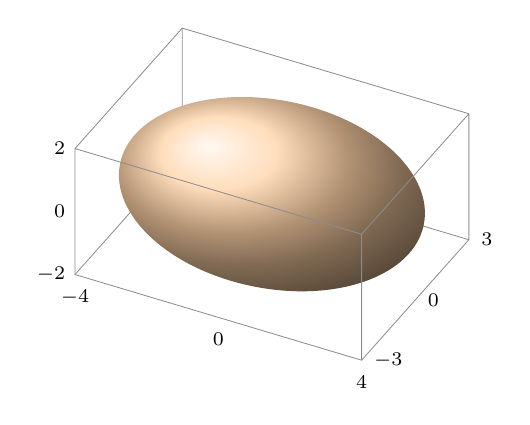
\begin{tikzpicture}[x={(0.455cm,-0.136cm)},y={(0.227cm,0.255cm)},z={(0cm,0.4cm)},
    font=\scriptsize,edge/.style={black!45,line width=.3pt}]
  \draw[edge] (4,3,-2)--(-4,3,-2)--(-4,-3,-2) (-4,3,-2)--(-4,3,2);
  \shade[ball color=orange!35!white,rotate=-11.3] (0,0) ellipse
    [x radius=1.967cm,y radius=1.195cm];
  \draw[edge] (-4,-3,-2)--(4,-3,-2)--(4,3,-2)--(4,3,2)--(-4,3,2)--(-4,-3,2)--cycle
    (4,-3,-2)--(4,-3,2)--(4,3,2) (4,-3,2)--(-4,-3,2);
  \foreach \z in {-2,0,2} \node[left] at (-4,-3,\z) {$\z$};
  \foreach \x in {-4,0,4} \node[below=2pt] at (\x,-3,-2) {$\x$};
  \foreach \y in {-3,0,3} \node[right=1pt] at (4,\y,-2) {$\y$};
\end{tikzpicture}
\end{minipage}\hfill
\begin{minipage}[c]{.36\linewidth}\centering
\captionof*{figure}{The ellipsoid $E(4f_1,3f_2,2f_3)$ in $\R^3$, where
$f_1,f_2,f_3$ is the standard basis of $\R^3$.}
\end{minipage}
\end{center}
\end{example}

The ellipsoid $E(f_1,\dots,f_n)$ equals the ball $B$ in $V$ for every
orthonormal basis $f_1,\dots,f_n$ of $V$ [by Parseval's identity
\ref{ax:6.30}(b)].

\begin{notation}[$T(\Omega)$]\label{ax:7.98}
For $T$ a function defined on $V$ and $\Omega\subseteq V$, define $T(\Omega)$
by
\[ T(\Omega) = \{Tv : v\in\Omega\}. \]
\end{notation}

Thus if $T$ is a function defined on $V$, then $T(V)=\range T$.

The next result states that every invertible operator $T\in\Lin(V)$ maps the
ball $B$ in $V$ onto an ellipsoid in $V$. The proof shows that the principal
axes of this ellipsoid come from the singular value decomposition of $T$.

\begin{result}[Invertible operator takes ball to ellipsoid]\label{ax:7.99}
Suppose $T\in\Lin(V)$ is invertible. Then $T$ maps the ball $B$ in $V$ onto an
ellipsoid in $V$.
\end{result}

\begin{proof}
Suppose $T$ has singular value decomposition
\[ Tv = s_1\ip{v}{e_1}f_1+\cdots+s_n\ip{v}{e_n}f_n \axeqno\label{ax:7.100} \]
for all $v\in V$; here $s_1,\dots,s_n$ are the singular values of $T$ and
$e_1,\dots,e_n$ and $f_1,\dots,f_n$ are both orthonormal bases of $V$. We will
show that $T(B)=E(s_1f_1,\dots,s_nf_n)$.

First suppose $v\in B$. Because $T$ is invertible, none of the singular values
$s_1,\dots,s_n$ equals $0$ (see \ref{ax:7.68}). Thus \ref{ax:7.100} implies
that
\[ \frac{\abs{\ip{Tv}{f_1}}^2}{s_1^2}+\cdots+\frac{\abs{\ip{Tv}{f_n}}^2}{s_n^2}
   = \abs{\ip{v}{e_1}}^2+\cdots+\abs{\ip{v}{e_n}}^2 < 1. \]
Thus $Tv\in E(s_1f_1,\dots,s_nf_n)$. Hence $T(B)\subseteq
E(s_1f_1,\dots,s_nf_n)$.

To prove inclusion in the other direction, now suppose
$w\in E(s_1f_1,\dots,s_nf_n)$. Let
\[ v = \frac{\ip{w}{f_1}}{s_1}e_1+\cdots+\frac{\ip{w}{f_n}}{s_n}e_n. \]
Then $\norm{v}<1$ and \ref{ax:7.100} implies that
$Tv=\ip{w}{f_1}f_1+\cdots+\ip{w}{f_n}f_n=w$. Thus
$T(B)\supseteq E(s_1f_1,\dots,s_nf_n)$.
\end{proof}

We now use the previous result to show that invertible operators take all
ellipsoids, not just the ball of radius $1$, to ellipsoids.

\begin{result}[Invertible operator takes ellipsoids to ellipsoids]\label{ax:7.101}
Suppose $T\in\Lin(V)$ is invertible and $E$ is an ellipsoid in $V$. Then
$T(E)$ is an ellipsoid in $V$.
\end{result}

\begin{proof}
There exist an orthonormal basis $f_1,\dots,f_n$ of $V$ and positive numbers
$s_1,\dots,s_n$ such that $E=E(s_1f_1,\dots,s_nf_n)$. Define $S\in\Lin(V)$ by
\[ S(a_1f_1+\cdots+a_nf_n) = a_1s_1f_1+\cdots+a_ns_nf_n. \]
Then $S$ maps the ball $B$ of $V$ onto $E$, as you can verify. Thus
\[ T(E) = T\bigl(S(B)\bigr) = (TS)(B). \]
The equation above and \ref{ax:7.99}, applied to $TS$, show that $T(E)$ is an
ellipsoid in $V$.
\end{proof}

Recall (see \ref{ax:3.95}) that if $u\in V$ and $\Omega\subseteq V$ then
$u+\Omega$ is defined by
\[ u+\Omega = \{u+w : w\in\Omega\}. \]
Geometrically, the sets $\Omega$ and $u+\Omega$ look the same, but they are in
different locations.

In the following definition, if $\dim V=2$ then the word
\emph{parallelogram} is often used instead of \emph{parallelepiped}.

\begin{definition}[$P(v_1,\dots,v_n)$, parallelepiped]\label{ax:7.102}
Suppose $v_1,\dots,v_n$ is a basis of $V$. Let
\[ P(v_1,\dots,v_n) = \{a_1v_1+\cdots+a_nv_n : a_1,\dots,a_n\in(0,1)\}. \]
A \emph{parallelepiped} is a set of the form $u+P(v_1,\dots,v_n)$ for some
$u\in V$. The vectors $v_1,\dots,v_n$ are called the \emph{edges} of this
parallelepiped.
\end{definition}

\begin{example}[Parallelepipeds]\label{ax:7.103}\leavevmode
\begin{center}
\begin{minipage}[b]{.48\linewidth}\centering
\begin{tikzpicture}[xscale=1.3,yscale=1.3]
  \fill[axfigblue] (.3,.5)--(1.3,.5)--(2.3,1.5)--(1.3,1.5)--cycle;
  \draw[line width=.4pt] (-.15,0)--(2.45,0); \draw[line width=.4pt] (-.15,0)--(-.15,1.6);
  \foreach \t in {0.3,1.3,2.3}
    \draw (\t,0)--(\t,-.06) node[below,font=\scriptsize] {$\t$};
  \foreach \t in {0.5,1.5}
    \draw (-.15,\t)--(-.21,\t) node[left,font=\scriptsize] {$\t$};
  \draw[vec] (.3,.5)--node[below,font=\scriptsize]{$v_1$} (1.3,.5);
  \draw[vec] (.3,.5)--node[above left=-1pt,font=\scriptsize]{$v_2$} (1.3,1.5);
\end{tikzpicture}
\captionof*{figure}{The parallelepiped $(0.3,0.5)+P\bigl((1,0),(1,1)\bigr)$
in $\R^2$.}
\end{minipage}\hfill
\begin{minipage}[b]{.48\linewidth}\centering
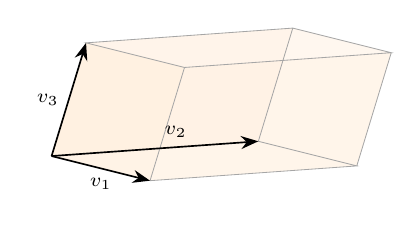
\begin{tikzpicture}[scale=1.25]
  \coordinate (O) at (0,0); \coordinate (a) at (1,-.25);
  \coordinate (b) at (2.1,.15); \coordinate (c) at (.35,1.15);
  \fill[orange!12,opacity=.8] (O)--(b)--($(b)+(c)$)--(c)--cycle;
  \fill[orange!12,opacity=.8] (O)--(a)--($(a)+(c)$)--(c)--cycle;
  \fill[orange!8,opacity=.8] (c)--($(a)+(c)$)--($(a)+(b)+(c)$)--($(b)+(c)$)--cycle;
  \fill[orange!10,opacity=.8] (a)--($(a)+(b)$)--($(a)+(b)+(c)$)--($(a)+(c)$)--cycle;
  \draw[black!35,line width=.3pt] (a)--($(a)+(b)$)--(b) (c)--($(a)+(c)$)
    --($(a)+(b)+(c)$)--($(b)+(c)$)--cycle ($(a)+(c)$)--(a)
    ($(a)+(b)$)--($(a)+(b)+(c)$) (b)--($(b)+(c)$);
  \draw[vec] (O)--node[below,font=\scriptsize]{$v_1$} (a);
  \draw[vec] (O)--node[above,pos=.6,font=\scriptsize]{$v_2$} (b);
  \draw[vec] (O)--node[left,font=\scriptsize]{$v_3$} (c);
\end{tikzpicture}
\captionof*{figure}{A parallelepiped in $\R^3$.}
\end{minipage}
\end{center}
\end{example}

\begin{result}[Invertible operator takes parallelepipeds to
parallelepipeds]\label{ax:7.104}
Suppose $u\in V$, $v_1,\dots,\allowbreak v_n$ is a basis of $V$, and
$T\in\Lin(V)$ is invertible. Then
\[ T\bigl(u+P(v_1,\dots,v_n)\bigr) = Tu+P(Tv_1,\dots,Tv_n). \]
\end{result}

\begin{proof}
Because $T$ is invertible, the list $Tv_1,\dots,Tv_n$ is a basis of $V$. The
linearity of $T$ implies that
\[ T(u+a_1v_1+\cdots+a_nv_n) = Tu+a_1Tv_1+\cdots+a_nTv_n \]
for all $a_1,\dots,a_n\in(0,1)$. Thus
$T\bigl(u+P(v_1,\dots,v_n)\bigr)=Tu+P(Tv_1,\dots,Tv_n)$.
\end{proof}

Just as the rectangles are distinguished among the parallelograms in $\R^2$, we
give a special name to the parallelepipeds in $V$ whose defining edges are
orthogonal to each other.

\begin{definition}[Box]\label{ax:7.105}
A \emph{box} in $V$ is a set of the form
\[ u+P(r_1e_1,\dots,r_ne_n), \]
where $u\in V$ and $r_1,\dots,r_n$ are positive numbers and $e_1,\dots,e_n$ is
an orthonormal basis of $V$.
\end{definition}

Note that in the special case of $\R^2$ each box is a rectangle, but the
terminology \emph{box} can be used in all dimensions.

\begin{example}[Boxes]\label{ax:7.106}\leavevmode
\begin{center}
\begin{minipage}[b]{.48\linewidth}\centering
\begin{tikzpicture}[scale=1]
  \fill[axfigblue] (1,0)--(2,1)--(1,2)--(0,1)--cycle;
  \draw[line width=.4pt] (-.05,-.1)--(2.15,-.1); \draw[line width=.4pt] (-.05,-.1)--(-.05,2.1);
  \foreach \t in {1,2} {
    \draw (\t,-.1)--(\t,-.16) node[below,font=\scriptsize] {$\t$};
    \draw (-.05,\t)--(-.11,\t) node[left,font=\scriptsize] {$\t$};}
  \draw[vec] (1,0)--node[below right=-1pt,pos=.5,font=\scriptsize]{$\sqrt2 e_1$} (2,1);
  \draw[vec] (1,0)--node[below left=-1pt,pos=.5,font=\scriptsize]{$\sqrt2 e_2$} (0,1);
\end{tikzpicture}
\captionof*{figure}{The box $(1,0)+P(\sqrt2e_1,\sqrt2e_2)$, where
$e_1=\bigl(1/\sqrt2,1/\sqrt2\bigr)$ and
$e_2=\bigl(-1/\sqrt2,1/\sqrt2\bigr)$.}
\end{minipage}\hfill
\begin{minipage}[b]{.48\linewidth}\centering
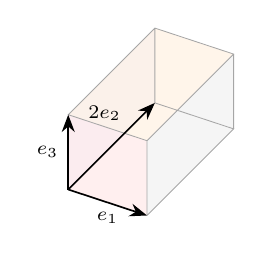
\begin{tikzpicture}[x={(1cm,-.33cm)},y={(.55cm,.55cm)},z={(0cm,.95cm)}]
  \fill[blue!8,opacity=.8] (0,0,0)--(0,2,0)--(0,2,1)--(0,0,1)--cycle;
  \fill[red!8,opacity=.8] (0,0,0)--(1,0,0)--(1,0,1)--(0,0,1)--cycle;
  \fill[orange!10,opacity=.8] (0,0,1)--(1,0,1)--(1,2,1)--(0,2,1)--cycle;
  \fill[black!5,opacity=.8] (1,0,0)--(1,2,0)--(1,2,1)--(1,0,1)--cycle;
  \draw[black!35,line width=.3pt] (1,0,0)--(1,2,0)--(0,2,0) (0,0,1)--(1,0,1)
    --(1,2,1)--(0,2,1)--cycle (1,0,0)--(1,0,1) (1,2,0)--(1,2,1) (0,2,0)--(0,2,1);
  \draw[vec] (0,0,0)--node[below,font=\scriptsize]{$e_1$} (1,0,0);
  \draw[vec] (0,0,0)--node[above left=-1pt,pos=.7,font=\scriptsize]{$2e_2$} (0,2,0);
  \draw[vec] (0,0,0)--node[left,font=\scriptsize]{$e_3$} (0,0,1);
\end{tikzpicture}
\captionof*{figure}{The box $P(e_1,2e_2,e_3)$, where $e_1,e_2,e_3$ is the
standard basis of $\R^3$.}
\end{minipage}
\end{center}
\end{example}

Suppose $T\in\Lin(V)$ is invertible. Then $T$ maps every parallelepiped in $V$
to a parallelepiped in $V$ (by \ref{ax:7.104}). In particular, $T$ maps every
box in $V$ to a parallelepiped in $V$. This raises the question of whether $T$
maps some boxes in $V$ to boxes in $V$. The following result answers this
question, with the help of the singular value decomposition.

\begin{result}[Every invertible operator takes some boxes to boxes]\label{ax:7.107}
Suppose $T\in\Lin(V)$ is invertible. Suppose $T$ has singular value
decomposition
\[ Tv = s_1\ip{v}{e_1}f_1+\cdots+s_n\ip{v}{e_n}f_n, \]
where $s_1,\dots,s_n$ are the singular values of $T$ and $e_1,\dots,e_n$ and
$f_1,\dots,f_n$ are orthonormal bases of $V$ and the equation above holds for
all $v\in V$. Then $T$ maps the box $u+P(r_1e_1,\dots,r_ne_n)$ onto the box
$Tu+P(r_1s_1f_1,\dots,r_ns_nf_n)$ for all positive numbers $r_1,\dots,r_n$ and
all $u\in V$.
\end{result}

\begin{proof}
If $a_1,\dots,a_n\in(0,1)$ and $r_1,\dots,r_n$ are positive numbers and
$u\in V$, then
\[ T(u+a_1r_1e_1+\cdots+a_nr_ne_n) = Tu+a_1r_1s_1f_1+\cdots+a_nr_ns_nf_n. \]
Thus $T\bigl(u+P(r_1e_1,\dots,r_ne_n)\bigr)=Tu+P(r_1s_1f_1,\dots,r_ns_nf_n)$.
\end{proof}

\subsection{Volume via Singular Values}

Our goal in this subsection is to understand how an operator changes the volume
of subsets of its domain. Because notions of volume belong to analysis rather
than to linear algebra, we will work only with an intuitive notion of volume.
Our intuitive approach to volume can be converted into appropriate correct
definitions, correct statements, and correct proofs using the machinery of
analysis.

Our intuition about volume works best in real inner product spaces. Thus the
assumption that $\F=\R$ will appear frequently in the rest of this subsection.

If $\dim V=n$, then by \emph{volume} we will mean $n$-dimensional volume. You
should be familiar with this concept in $\R^3$. When $n=2$, this is usually
called area instead of volume, but for consistency we use the word volume in
all dimensions. The most fundamental intuition about volume is that the volume
of a box (whose defining edges are by definition orthogonal to each other) is
the product of the lengths of the defining edges. Thus we make the following
definition.

\begin{definition}[Volume of a box]\label{ax:7.108}
Suppose $\F=\R$. If $u\in V$ and $r_1,\dots,r_n$ are positive numbers and
$e_1,\dots,e_n$ is an orthonormal basis of $V$, then
\[ \operatorname{volume}\bigl(u+P(r_1e_1,\dots,r_ne_n)\bigr)
   = r_1\times\cdots\times r_n. \]
\end{definition}

The definition above agrees with the familiar formulas for the area (which we
are calling the volume) of a rectangle in $\R^2$ and for the volume of a box in
$\R^3$. For example, the first box in Example~\ref{ax:7.106} has
two-dimensional volume (or area) $2$ because the defining edges of that box
have length $\sqrt2$ and $\sqrt2$. The second box in Example~\ref{ax:7.106}
has three-dimensional volume $2$ because the defining edges of that box have
length $1$, $2$, and $1$.

\marginfig{\begin{tikzpicture}[scale=.75]
  \fill[axfigblue] (0,0) circle (1);
  \draw[line width=.4pt] (-.68,-.68) rectangle (.68,.68)
    (.68,-.55) rectangle (.97,.55) (-.68,-.55) rectangle (-.97,.55)
    (-.55,.68) rectangle (.55,.97) (-.55,-.68) rectangle (.55,-.97);
\end{tikzpicture}}{Volume of this ball $\approx$ sum of the volumes of the five
boxes.}%
To define the volume of a subset of $V$, approximate the subset by a finite
collection of disjoint boxes, and then add up the volumes of the approximating
collection of boxes. As we approximate a subset of $V$ more accurately by
disjoint unions of more boxes, we get a better approximation to the volume.

These ideas should remind you of how the Riemann integral is defined by
approximating the area under a curve by a disjoint collection of rectangles.
This discussion leads to the following nonrigorous but intuitive definition.

\begin{definition}[Volume]\label{ax:7.109}
Suppose $\F=\R$ and $\Omega\subseteq V$. Then the \emph{volume} of $\Omega$,
denoted by $\operatorname{volume}\Omega$, is approximately the sum of the
volumes of a collection of disjoint boxes that approximate $\Omega$.
\end{definition}

\marginfig{\begin{tikzpicture}[xscale=1.5,yscale=.75]
  \fill[axfigblue] (0,0) circle (1);
  \draw[line width=.4pt] (-.68,-.68) rectangle (.68,.68)
    (.68,-.55) rectangle (.97,.55) (-.68,-.55) rectangle (-.97,.55)
    (-.55,.68) rectangle (.55,.97) (-.55,-.68) rectangle (.55,-.97);
\end{tikzpicture}}{Each box here has twice the width and the same height as
the boxes in the previous figure.}%
We are ignoring many reasonable questions by taking an intuitive approach to
volume. For example, if we approximate $\Omega$ by boxes with respect to one
basis, do we get the same volume if we approximate $\Omega$ by boxes with
respect to a different basis? If $\Omega_1$ and $\Omega_2$ are disjoint
subsets of $V$, is
$\operatorname{volume}(\Omega_1\cup\Omega_2)
=\operatorname{volume}\Omega_1+\operatorname{volume}\Omega_2$? Provided that
we consider only reasonably nice subsets of $V$, techniques of analysis show
that both these questions have affirmative answers that agree with our
intuition about volume.

\begin{example}[Volume change by a linear map]\label{ax:7.110}
Suppose that $T\in\Lin(\R^2)$ is defined by
$Tv=\allowbreak2\ip{v}{e_1}e_1+\ip{v}{e_2}e_2$, where $e_1,e_2$ is the standard basis of
$\R^2$. This linear map stretches vectors along the $e_1$-axis by a factor of
$2$ and leaves vectors along the $e_2$-axis unchanged. The ball approximated by
five boxes above gets mapped by $T$ to the ellipsoid shown here. Each of the
five boxes in the original figure gets mapped to a box of twice the width and
the same height as in the original figure. Hence each box gets mapped to a box
of twice the volume (area) as in the original figure. The sum of the volumes of
the five new boxes approximates the volume of the ellipsoid. Thus $T$ changes
the volume of the ball by a factor of $2$.
\end{example}

In the example above, $T$ maps boxes with respect to the basis $e_1,e_2$ to
boxes with respect to the same basis; thus we can see how $T$ changes volume.
In general, an operator maps boxes to parallelepipeds that are not boxes.
However, if we choose the right basis (coming from the singular value
decomposition!), then boxes with respect to that basis get mapped to boxes
with respect to a possibly different basis, as shown in \ref{ax:7.107}. This
observation leads to a natural proof of the following result.

\begin{result}[Volume changes by a factor of the product of the singular
values]\label{ax:7.111}
Suppose $\F=\R$, $T\in\Lin(V)$ is invertible, and $\Omega\subseteq V$. Then
\[ \operatorname{volume}T(\Omega)
   = (\text{product of singular values of }T)(\operatorname{volume}\Omega). \]
\end{result}

\begin{proof}
Suppose $T$ has singular value decomposition
\[ Tv = s_1\ip{v}{e_1}f_1+\cdots+s_n\ip{v}{e_n}f_n \]
for all $v\in V$, where $e_1,\dots,e_n$ and $f_1,\dots,f_n$ are orthonormal
bases of $V$.

Approximate $\Omega$ by boxes of the form $u+P(r_1e_1,\dots,r_ne_n)$, which
have volume $r_1\times\cdots\times r_n$. The operator $T$ maps each box
$u+P(r_1e_1,\dots,r_ne_n)$ onto the box $Tu+P(r_1s_1f_1,\dots,r_ns_nf_n)$,
which has volume $(s_1\times\cdots\times s_n)(r_1\times\cdots\times r_n)$.

The operator $T$ maps a collection of boxes that approximate $\Omega$ onto a
collection of boxes that approximate $T(\Omega)$. Because $T$ changes the
volume of each box in a collection that approximates $\Omega$ by a factor of
$s_1\times\cdots\times s_n$, the linear map $T$ changes the volume of $\Omega$
by the same factor.
\end{proof}

Suppose $T\in\Lin(V)$. As we will see when we get to determinants, the product
of the singular values of $T$ equals $\abs{\det T}$; see \ref{ax:9.60} and
\ref{ax:9.61}.

\subsection{Properties of an Operator as Determined by Its Eigenvalues}

We conclude this chapter by presenting the table below. The context of this
table is a finite-dimensional complex inner product space. The first column of
the table shows a property that a normal operator on such a space might have.
The second column of the table shows a subset of $\C$ such that the operator
has the corresponding property if and only if all eigenvalues of the operator
lie in the specified subset. For example, the first row of the table states
that a normal operator is invertible if and only if all its eigenvalues are
nonzero (this first row is the only one in the table that does not need the
hypothesis that the operator is normal).

Make sure you can explain why all results in the table hold. For example, the
last row of the table holds because the norm of an operator equals its largest
singular value (by \ref{ax:7.85}) and the singular values of a normal
operator, assuming $\F=\C$, equal the absolute values of the eigenvalues (by
Exercise~7 in Section~7E).

\begin{center}\small
\begin{tabular}{l|l}
\multicolumn{1}{l}{\textbf{properties of a normal operator}} &
  \multicolumn{1}{l}{\textbf{eigenvalues are contained in}}\\
\hline
invertible & $\C\setminus\{0\}$\\ \hline
self-adjoint & $\R$\\ \hline
skew & $\{\lambda\in\C : \Re\lambda=0\}$\\ \hline
orthogonal projection & $\{0,1\}$\\ \hline
positive & $[0,\infty)$\\ \hline
unitary & $\{\lambda\in\C : \abs{\lambda}=1\}$\\ \hline
norm is less than $1$ & $\{\lambda\in\C : \abs{\lambda}<1\}$\\ \hline
\end{tabular}
\end{center}

% ------------------------------------------------------------------ exercises
\exercisesheading{7F}

\begin{exercise}
Prove that if $S,T\in\Lin(V,W)$, then
$\bigl\lvert\norm{S}-\norm{T}\bigr\rvert\le\norm{S-T}$.
\exnote{The inequality above is called the \textbf{reverse triangle
inequality}.}
\end{exercise}

\begin{exercise}
Suppose that $T\in\Lin(V)$ is self-adjoint or that $\F=\C$ and $T\in\Lin(V)$
is normal. Prove that
\[ \norm{T} = \max\{\abs{\lambda} : \lambda \text{ is an eigenvalue of } T\}. \]
\end{exercise}

\begin{exercise}
Suppose $T\in\Lin(V,W)$ and $v\in V$. Prove that
\[ \norm{Tv}=\norm{T}\,\norm{v} \iff T^*Tv=\norm{T}^2v. \]
\end{exercise}

\begin{exercise}
Suppose $T\in\Lin(V,W)$, $v\in V$, and $\norm{Tv}=\norm{T}\,\norm{v}$. Prove
that if $u\in V$ and $\ip{u}{v}=0$, then $\ip{Tu}{Tv}=0$.
\end{exercise}

\begin{exercise}
Suppose $U$ is a finite-dimensional inner product space, $T\in\Lin(V,U)$, and
$S\in\Lin(U,W)$. Prove that
\[ \norm{ST}\le\norm{S}\,\norm{T}. \]
\end{exercise}

\begin{exercise}
Prove or give a counterexample: If $S,T\in\Lin(V)$, then
$\norm{ST}=\norm{TS}$.
\end{exercise}

\begin{exercise}
Show that defining $d(S,T)=\norm{S-T}$ for $S,T\in\Lin(V,W)$ makes $d$ a
metric on $\Lin(V,W)$.
\exnote{This exercise is intended for readers who are familiar with metric
spaces.}
\end{exercise}

\begin{exercise}\leavevmode
\begin{parts}
\item Prove that if $T\in\Lin(V)$ and $\norm{I-T}<1$, then $T$ is invertible.
\item Suppose that $S\in\Lin(V)$ is invertible. Prove that if $T\in\Lin(V)$
  and $\norm{S-T}<1/\norm{S^{-1}}$, then $T$ is invertible.
\end{parts}
\exnote{This exercise shows that the set of invertible operators in $\Lin(V)$
is an open subset of $\Lin(V)$, using the metric defined in Exercise~7.}
\end{exercise}

\begin{exercise}
Suppose $T\in\Lin(V)$. Prove that for every $\epsilon>0$, there exists an
invertible operator $S\in\Lin(V)$ such that $0<\norm{T-S}<\epsilon$.
\end{exercise}

\begin{exercise}
Suppose $\dim V>1$ and $T\in\Lin(V)$ is not invertible. Prove that for every
$\epsilon>0$, there exists $S\in\Lin(V)$ such that $0<\norm{T-S}<\epsilon$ and
$S$ is not invertible.
\end{exercise}

\begin{exercise}
Suppose $\F=\C$ and $T\in\Lin(V)$. Prove that for every $\epsilon>0$ there
exists a diagonalizable operator $S\in\Lin(V)$ such that
$0<\norm{T-S}<\epsilon$.
\end{exercise}

\begin{exercise}
Suppose $T\in\Lin(V)$ is a positive operator. Show that
$\bigl\lVert\sqrt{T}\bigr\rVert=\sqrt{\norm{T}}$.
\end{exercise}

\begin{exercise}
Suppose $S,T\in\Lin(V)$ are positive operators. Show that
\[ \norm{S-T}\le\max\{\norm{S},\norm{T}\}\le\norm{S+T}. \]
\end{exercise}

\begin{exercise}
Suppose $U$ and $W$ are subspaces of $V$ such that $\norm{P_U-P_W}<1$. Prove
that $\dim U=\dim W$.
\end{exercise}

\begin{exercise}
Define $T\in\Lin(\F^3)$ by
\[ T(z_1,z_2,z_3) = (z_3,2z_1,3z_2). \]
Find (explicitly) a unitary operator $S\in\Lin(\F^3)$ such that
$T=S\sqrt{T^*T}$.
\end{exercise}

\begin{exercise}
Suppose $S\in\Lin(V)$ is a positive invertible operator. Prove that there
exists $\delta>0$ such that $T$ is a positive operator for every self-adjoint
operator $T\in\Lin(V)$ with $\norm{S-T}<\delta$.
\end{exercise}

\begin{exercise}
Prove that if $u\in V$ and $\varphi_u$ is the linear functional on $V$ defined
by the equation $\varphi_u(v)=\ip{v}{u}$, then $\norm{\varphi_u}=\norm{u}$.
\exnote{Here we are thinking of the scalar field $\F$ as an inner product
space with $\ip{\alpha}{\beta}=\alpha\overline{\beta}$ for all
$\alpha,\beta\in\F$. Thus $\norm{\varphi_u}$ means the norm of $\varphi_u$ as a
linear map from $V$ to $\F$.}
\end{exercise}

\begin{exercise}
Suppose $e_1,\dots,e_n$ is an orthonormal basis of $V$ and $T\in\Lin(V,W)$.
\begin{parts}
\item Prove that
  $\max\{\norm{Te_1},\dots,\norm{Te_n}\}\le\norm{T}
  \le(\norm{Te_1}^2+\cdots+\norm{Te_n}^2)^{1/2}$.
\item Prove that $\norm{T}=(\norm{Te_1}^2+\cdots+\norm{Te_n}^2)^{1/2}$
  if and only if $\dim\range T\le1$.
\end{parts}
\exnote{Here $e_1,\dots,e_n$ is an arbitrary orthonormal basis of $V$, not
necessarily connected with a singular value decomposition of $T$. If
$s_1,\dots,s_n$ is the list of singular values of $T$, then the right side of
the inequality above equals $(s_1^2+\cdots+s_n^2)^{1/2}$, as was shown in
Exercise~11(a) in Section~7E.}
\end{exercise}

\begin{exercise}
Prove that if $T\in\Lin(V,W)$, then $\norm{T^*T}=\norm{T}^2$.
\exnote{This formula for $\norm{T^*T}$ leads to the important subject of
$C^*$-algebras.}
\end{exercise}

\begin{exercise}
Suppose $T\in\Lin(V)$ is normal. Prove that $\norm{T^k}=\norm{T}^k$ for every
positive integer $k$.
\end{exercise}

\begin{exercise}
Suppose $\dim V>1$ and $\dim W>1$. Prove that the norm on $\Lin(V,W)$ does not
come from an inner product. In other words, prove that there does not exist an
inner product on $\Lin(V,W)$ such that
\[ \max\{\norm{Tv} : v\in V \text{ and } \norm{v}\le1\} = \sqrt{\ip{T}{T}} \]
for all $T\in\Lin(V,W)$.
\end{exercise}

\begin{exercise}
Suppose $T\in\Lin(V,W)$. Let $n=\dim V$ and let $s_1\ge\cdots\ge s_n$ denote
the singular values of $T$. Prove that if $1\le k\le n$, then
\[ \min\{\norm{T|_U} : U \text{ is a subspace of } V \text{ with }
   \dim U=k\} = s_{n-k+1}. \]
\end{exercise}

\begin{exercise}
Suppose $T\in\Lin(V,W)$. Show that $T$ is uniformly continuous with respect to
the metrics on $V$ and $W$ that arise from the norms on those spaces (see
Exercise~23 in Section~6B).
\end{exercise}

\begin{exercise}
Suppose $T\in\Lin(V)$ is invertible. Prove that
\[ \norm{T^{-1}}=\norm{T}^{-1} \iff \frac{T}{\norm{T}}
   \text{ is a unitary operator.} \]
\end{exercise}

\begin{exercise}
Fix $u,x\in V$ with $u\ne0$. Define $T\in\Lin(V)$ by $Tv=\ip{v}{u}x$ for every
$v\in V$. Prove that
\[ \sqrt{T^*T}\,v = \frac{\norm{x}}{\norm{u}}\ip{v}{u}u \]
for every $v\in V$.
\end{exercise}

\begin{exercise}
Suppose $T\in\Lin(V)$. Prove that $T$ is invertible if and only if there
exists a unique unitary operator $S\in\Lin(V)$ such that $T=S\sqrt{T^*T}$.
\end{exercise}

\begin{exercise}
Suppose $T\in\Lin(V)$ and $s_1,\dots,s_n$ are the singular values of $T$. Let
$e_1,\dots,e_n$ and $f_1,\dots,f_n$ be orthonormal bases of $V$ such that
\[ Tv = s_1\ip{v}{e_1}f_1+\cdots+s_n\ip{v}{e_n}f_n \]
for all $v\in V$. Define $S\in\Lin(V)$ by
\[ Sv = \ip{v}{e_1}f_1+\cdots+\ip{v}{e_n}f_n. \]
\begin{parts}
\item Show that $S$ is unitary and
  $\norm{T-S}=\max\{\abs{s_1-1},\dots,\abs{s_n-1}\}$.
\item Show that if $E\in\Lin(V)$ is unitary, then $\norm{T-E}\ge\norm{T-S}$.
\end{parts}
\exnote{This exercise finds a unitary operator $S$ that is as close as
possible (among the unitary operators) to a given operator $T$.}
\end{exercise}

\begin{exercise}
Suppose $T\in\Lin(V)$. Prove that there exists a unitary operator
$S\in\Lin(V)$ such that $T=\sqrt{TT^*}\,S$.
\end{exercise}

\begin{exercise}
Suppose $T\in\Lin(V)$.
\begin{parts}
\item Use the polar decomposition to show that there exists a unitary operator
  $S\in\Lin(V)$ such that $TT^*=ST^*TS^*$.
\item Show how (a) implies that $T$ and $T^*$ have the same singular values.
\end{parts}
\end{exercise}

\begin{exercise}
Suppose $T\in\Lin(V)$, $S\in\Lin(V)$ is a unitary operator, and $R\in\Lin(V)$
is a positive operator such that $T=SR$. Prove that $R=\sqrt{T^*T}$.
\exnote{This exercise shows that if we write $T$ as the product of a unitary
operator and a positive operator (as in the polar decomposition
\ref{ax:7.93}), then the positive operator equals $\sqrt{T^*T}$.}
\end{exercise}

\begin{exercise}
Suppose $\F=\C$ and $T\in\Lin(V)$ is normal. Prove that there exists a unitary
operator $S\in\Lin(V)$ such that $T=S\sqrt{T^*T}$ and such that $S$ and
$\sqrt{T^*T}$ both have diagonal matrices with respect to the same orthonormal
basis of $V$.
\end{exercise}

\begin{exercise}
Suppose that $T\in\Lin(V,W)$ and $T\ne0$. Let $s_1,\dots,s_m$ denote the
positive singular values of $T$. Show that there exists an orthonormal basis
$e_1,\dots,e_m$ of $(\nul T)^\perp$ such that
\[ T\Bigl(E\Bigl(\frac{e_1}{s_1},\dots,\frac{e_m}{s_m}\Bigr)\Bigr) \]
equals the ball in $\range T$ of radius $1$ centered at $0$.
\end{exercise}



\part{Structure}
% Chapter 8: assembled from chapters/ch08/*.tex
% Source: book p. 297 (PDF 311).
\chapter{Operators on Complex Vector Spaces}

In this chapter we delve deeper into the structure of operators, with most of
the attention on complex vector spaces. Some of the results in this chapter
apply to both real and complex vector spaces; thus we do not make a standing
assumption that $\F=\C$. Also, an inner product does not help with this
material, so we return to the general setting of a finite-dimensional vector
space.

Even on a finite-dimensional complex vector space, an operator may not have
enough eigenvectors to form a basis of the vector space. Thus we will consider
the closely related objects called generalized eigenvectors. We will see that
for each operator on a finite-dimensional complex vector space, there is a basis
of the vector space consisting of generalized eigenvectors of the operator. The
generalized eigenspace decomposition then provides a good description of
arbitrary operators on a finite-dimensional complex vector space.

Nilpotent operators, which are operators that when raised to some power equal
$0$, have an important role in these investigations. Nilpotent operators provide
a key tool in our proof that every invertible operator on a finite-dimensional
complex vector space has a square root and in our approach to Jordan form.

This chapter concludes by defining the trace and proving its key properties.

\begin{definition*}[Standing assumptions for this chapter]\leavevmode
\begin{itemize}
\item $\F$ denotes $\R$ or $\C$.
\item $V$ denotes a finite-dimensional nonzero vector space over $\F$.
\end{itemize}
\end{definition*}

% Source: book pp. 298--307 (PDF 312--321). No solutions.
% numbered displays (Axler's 8.5, 8.7, ...): step the item counter and label
% it just before the display, then \tag*{\thetheorem} inside the display
\DeclareRobustCommand\axeqnum[1]{\refstepcounter{theorem}\label{ax:#1}}
% the italic comment that follows some exercises

\section{Generalized Eigenvectors and Nilpotent Operators}

\subsection{Null Spaces of Powers of an Operator}

We begin this chapter with a study of null spaces of powers of an operator.

\begin{result}[Sequence of increasing null spaces]\label{ax:8.1}
Suppose $T\in\Lin(V)$. Then
\[ \{0\} = \nul T^0 \subseteq \nul T^1 \subseteq \cdots \subseteq \nul T^k
   \subseteq \nul T^{k+1} \subseteq \cdots. \]
\end{result}

\begin{proof}
Suppose $k$ is a nonnegative integer and $v\in\nul T^k$. Then $T^kv=0$, which
implies that $T^{k+1}v=T(T^kv)=T(0)=0$. Thus $v\in\nul T^{k+1}$. Hence
$\nul T^k\subseteq\nul T^{k+1}$, as desired.
\end{proof}

\marginnote{For similar results about decreasing sequences of ranges, see
Exercises 6, 7, and 8.}%
The following result states that if two consecutive terms in the sequence of
subspaces above are equal, then all later terms in the sequence are equal.

\begin{result}[Equality in the sequence of null spaces]\label{ax:8.2}
Suppose $T\in\Lin(V)$ and $m$ is a nonnegative integer such that
\[ \nul T^m = \nul T^{m+1}. \]
Then
\[ \nul T^m = \nul T^{m+1} = \nul T^{m+2} = \nul T^{m+3} = \cdots. \]
\end{result}

\begin{proof}
Let $k$ be a positive integer. We want to prove that
\[ \nul T^{m+k} = \nul T^{m+k+1}. \]
We already know from \ref{ax:8.1} that $\nul T^{m+k}\subseteq\nul T^{m+k+1}$.

To prove the inclusion in the other direction, suppose $v\in\nul T^{m+k+1}$.
Then
\[ T^{m+1}(T^kv) = T^{m+k+1}v = 0. \]
Hence
\[ T^kv\in\nul T^{m+1} = \nul T^m. \]
Thus $T^{m+k}v=T^m(T^kv)=0$, which means that $v\in\nul T^{m+k}$. This implies
that $\nul T^{m+k+1}\subseteq\nul T^{m+k}$, completing the proof.
\end{proof}

The result above raises the question of whether there exists a nonnegative
integer $m$ such that $\nul T^m=\nul T^{m+1}$. The next result shows that this
equality holds at least when $m$ equals the dimension of the vector space on
which $T$ operates.

\begin{result}[Null spaces stop growing]\label{ax:8.3}
Suppose $T\in\Lin(V)$. Then
\[ \nul T^{\dim V} = \nul T^{\dim V+1} = \nul T^{\dim V+2} = \cdots. \]
\end{result}

\begin{proof}\emergencystretch=1.5em
We only need to prove that $\nul T^{\dim V}=\nul T^{\dim V+1}$ (by
\ref{ax:8.2}). Suppose this is not true. Then, by \ref{ax:8.1} and
\ref{ax:8.2}, we have
\[ \{0\} = \nul T^0 \subsetneq \nul T^1 \subsetneq \cdots \subsetneq
   \nul T^{\dim V} \subsetneq \nul T^{\dim V+1}, \]
where the symbol $\subsetneq$ means ``contained in but not equal to''. At each
of the strict inclusions in the chain above, the dimension increases by at
least $1$. Thus $\dim\nul T^{\dim V+1}\ge\dim V+1$, a contradiction because a
subspace of $V$ cannot have a larger dimension than $\dim V$.
\end{proof}

It is not true that $V=\nul T\oplus\range T$ for every $T\in\Lin(V)$. However,
the next result can be a useful substitute.

\begin{result}[$V$ is the direct sum of $\nul T^{\dim V}$ and
$\range T^{\dim V}$]\label{ax:8.4}
Suppose $T\in\Lin(V)$. Then
\[ V = \nul T^{\dim V}\oplus\range T^{\dim V}. \]
\end{result}

\begin{proof}
Let $n=\dim V$. First we show that\axeqnum{8.5}%
\[ (\nul T^n)\cap(\range T^n) = \{0\}. \tag*{\thetheorem} \]
Suppose $v\in(\nul T^n)\cap(\range T^n)$. Then $T^nv=0$, and there exists
$u\in V$ such that $v=T^nu$. Applying $T^n$ to both sides of the last equation
shows that $T^nv=T^{2n}u$. Hence $T^{2n}u=0$, which implies that $T^nu=0$ (by
\ref{ax:8.3}). Thus $v=T^nu=0$, completing the proof of \ref{ax:8.5}.

Now \ref{ax:8.5} implies that $\nul T^n+\range T^n$ is a direct sum (by
\ref{ax:1.46}). Also,
\[ \dim(\nul T^n\oplus\range T^n) = \dim\nul T^n+\dim\range T^n = \dim V, \]
where the first equality above comes from \ref{ax:3.94} and the second equality
comes from the fundamental theorem of linear maps (\ref{ax:3.21}). The equation
above implies that $\nul T^n\oplus\range T^n=V$ (see \ref{ax:2.39}), as
desired.
\end{proof}

For an improvement of the result above, see Exercise 19.

\begin{example}[$\F^3=\nul T^3\oplus\range T^3$ for $T\in\Lin(\F^3)$]\label{ax:8.6}
Suppose $T\in\Lin(\F^3)$ is defined by
\[ T(z_1,z_2,z_3) = (4z_2,0,5z_3). \]
Then $\nul T=\{(z_1,0,0) : z_1\in\F\}$ and
$\range T=\{(z_1,0,z_3) : z_1,z_3\in\F\}$. Thus $\nul T\cap\range T\ne\{0\}$.
Hence $\nul T+\range T$ is not a direct sum. Also note that
$\nul T+\range T\ne\F^3$. However, we have $T^3(z_1,z_2,z_3)=(0,0,125z_3)$.
Thus we see that
\[ \nul T^3 = \{(z_1,z_2,0) : z_1,z_2\in\F\} \quad\text{and}\quad
   \range T^3 = \{(0,0,z_3) : z_3\in\F\}. \]
Hence $\F^3=\nul T^3\oplus\range T^3$, as expected by \ref{ax:8.4}.
\end{example}

\subsection{Generalized Eigenvectors}

Some operators do not have enough eigenvectors to lead to good descriptions of
their behavior. Thus in this subsection we introduce the concept of generalized
eigenvectors, which will play a major role in our description of the structure
of an operator.

To understand why we need more than eigenvectors, let's examine the question of
describing an operator by decomposing its domain into invariant subspaces. Fix
$T\in\Lin(V)$. We seek to describe $T$ by finding a ``nice'' direct sum
decomposition
\[ V = V_1\oplus\cdots\oplus V_n, \]
where each $V_k$ is a subspace of $V$ invariant under $T$. The simplest
possible nonzero invariant subspaces are one-dimensional. A decomposition as
above in which each $V_k$ is a one-dimensional subspace of $V$ invariant under
$T$ is possible if and only if $V$ has a basis consisting of eigenvectors of
$T$ (see \ref{ax:5.55}). This happens if and only if $V$ has an eigenspace
decomposition\axeqnum{8.7}%
\[ V = E(\lambda_1,T)\oplus\cdots\oplus E(\lambda_m,T), \tag*{\thetheorem} \]
where $\lambda_1,\dots,\lambda_m$ are the distinct eigenvalues of $T$ (see
\ref{ax:5.55}).

The spectral theorem in the previous chapter shows that if $V$ is an inner
product space, then a decomposition of the form \ref{ax:8.7} holds for every
self-adjoint operator if $\F=\R$ and for every normal operator if $\F=\C$
because operators of those types have enough eigenvectors to form a basis of
$V$ (see \ref{ax:7.29} and \ref{ax:7.31}).

However, a decomposition of the form \ref{ax:8.7} may not hold for more general
operators, even on a complex vector space. An example was given by the operator
in \ref{ax:5.57}, which does not have enough eigenvectors for \ref{ax:8.7} to
hold. Generalized eigenvectors and generalized eigenspaces, which we now
introduce, will remedy this situation.

\begin{definition}[Generalized eigenvector]\label{ax:8.8}
Suppose $T\in\Lin(V)$ and $\lambda$ is an eigenvalue of $T$. A vector $v\in V$
is called a \emph{generalized eigenvector} of $T$ corresponding to $\lambda$ if
$v\ne0$ and
\[ (T-\lambda I)^kv = 0 \]
for some positive integer $k$.
\end{definition}

\marginnote{Generalized eigenvalues are not defined because doing so would not
lead to anything new. Reason: if $(T-\lambda I)^k$ is not injective for some
positive integer $k$, then $T-\lambda I$ is not injective, and hence $\lambda$
is an eigenvalue of $T$.}%
A nonzero vector $v\in V$ is a generalized eigenvector of $T$ corresponding to
$\lambda$ if and only if
\[ (T-\lambda I)^{\dim V}v = 0, \]
as follows from applying \ref{ax:8.1} and \ref{ax:8.3} to the operator
$T-\lambda I$.

As we know, an operator on a complex vector space may not have enough
eigenvectors to form a basis of the domain. The next result shows that on a
complex vector space there are enough generalized eigenvectors to do this.

\begin{result}[A basis of generalized eigenvectors]\label{ax:8.9}
Suppose $\F=\C$ and $T\in\Lin(V)$. Then there is a basis of $V$ consisting of
generalized eigenvectors of $T$.
\end{result}

\begin{proof}
Let $n=\dim V$. We will use induction on $n$. To get started, note that the
desired result holds if $n=1$ because then every nonzero vector in $V$ is an
eigenvector of $T$.

\marginnote{This step is where we use the hypothesis that $\F=\C$, because if
$\F=\R$ then $T$ may not have any eigenvalues.}%
Now suppose $n>1$ and the desired result holds for all smaller values of
$\dim V$. Let $\lambda$ be an eigenvalue of $T$. Applying \ref{ax:8.4} to
$T-\lambda I$ shows that
\[ V = \nul(T-\lambda I)^n\oplus\range(T-\lambda I)^n. \]

If $\nul(T-\lambda I)^n=V$, then every nonzero vector in $V$ is a generalized
eigenvector of $T$, and thus in this case there is a basis of $V$ consisting
of generalized eigenvectors of $T$. Hence we can assume that
$\nul(T-\lambda I)^n\ne V$, which implies that
$\range(T-\lambda I)^n\ne\{0\}$.

Also, $\nul(T-\lambda I)^n\ne\{0\}$, because $\lambda$ is an eigenvalue of $T$.
Thus we have
\[ 0 < \dim\range(T-\lambda I)^n < n. \]
Furthermore, $\range(T-\lambda I)^n$ is invariant under $T$
$\bigl[$by \ref{ax:5.18} with $p(z)=(z-\lambda)^n\bigr]$. Let
$S\in\Lin\bigl(\range(T-\lambda I)^n\bigr)$ equal $T$ restricted to
$\range(T-\lambda I)^n$. Our induction hypothesis applied to the operator $S$
implies that there is a basis of $\range(T-\lambda I)^n$ consisting of
generalized eigenvectors of $S$, which of course are generalized eigenvectors
of $T$. Adjoining that basis of $\range(T-\lambda I)^n$ to a basis of
$\nul(T-\lambda I)^n$ gives a basis of $V$ consisting of generalized
eigenvectors of $T$.
\end{proof}

If $\F=\R$ and $\dim V>1$, then some operators on $V$ have the property that
there exists a basis of $V$ consisting of generalized eigenvectors of the
operator, and (unlike what happens when $\F=\C$) other operators do not have
this property. See Exercise 11 for a necessary and sufficient condition that
determines whether an operator has this property.

\begin{example}[Generalized eigenvectors of an operator on $\C^3$]\label{ax:8.10}
Define $T\in\Lin(\C^3)$ by
\[ T(z_1,z_2,z_3) = (4z_2,0,5z_3) \]
for each $(z_1,z_2,z_3)\in\C^3$. A routine use of the definition of eigenvalue
shows that the eigenvalues of $T$ are $0$ and $5$. Furthermore, the
eigenvectors corresponding to the eigenvalue $0$ are the nonzero vectors of the
form $(z_1,0,0)$, and the eigenvectors corresponding to the eigenvalue $5$ are
the nonzero vectors of the form $(0,0,z_3)$. Hence this operator does not have
enough eigenvectors to span its domain $\C^3$.

We compute that $T^3(z_1,z_2,z_3)=(0,0,125z_3)$. Thus \ref{ax:8.1} and
\ref{ax:8.3} imply that the generalized eigenvectors of $T$ corresponding to the
eigenvalue $0$ are the nonzero vectors of the form $(z_1,z_2,0)$.

We also have $(T-5I)^3(z_1,z_2,z_3)=(-125z_1+300z_2,-125z_2,0)$. Thus the
generalized eigenvectors of $T$ corresponding to the eigenvalue $5$ are the
nonzero vectors of the form $(0,0,z_3)$.

The paragraphs above show that each of the standard basis vectors of $\C^3$ is a
generalized eigenvector of $T$. Thus $\C^3$ indeed has a basis consisting of
generalized eigenvectors of $T$, as promised by \ref{ax:8.9}.
\end{example}

If $v$ is an eigenvector of $T\in\Lin(V)$, then the corresponding eigenvalue
$\lambda$ is uniquely determined by the equation $Tv=\lambda v$, which can be
satisfied by only one $\lambda\in\F$ (because $v\ne0$). However, if $v$ is a
generalized eigenvector of $T$, then it is not obvious that the equation
$(T-\lambda I)^{\dim V}v=0$ can be satisfied by only one $\lambda\in\F$.
Fortunately, the next result tells us that all is well on this issue.

\begin{result}[Generalized eigenvector corresponds to a unique
eigenvalue]\label{ax:8.11}
Suppose $T\in\Lin(V)$. Then each generalized eigenvector of $T$ corresponds to
only one eigenvalue of $T$.
\end{result}

\begin{proof}
Suppose $v\in V$ is a generalized eigenvector of $T$ corresponding to
eigenvalues $\alpha$ and $\lambda$ of $T$. Let $m$ be the smallest positive
integer such that $(T-\alpha I)^mv=0$. Let $n=\dim V$. Then
\begin{align*}
0 &= (T-\lambda I)^nv\\
  &= \bigl((T-\alpha I)+(\alpha-\lambda)I\bigr)^nv\\
  &= \sum_{k=0}^{n} b_k(\alpha-\lambda)^{n-k}(T-\alpha I)^kv,
\end{align*}
where $b_0=1$ and the values of the other binomial coefficients $b_k$ do not
matter. Apply the operator $(T-\alpha I)^{m-1}$ to both sides of the equation
above, getting
\[ 0 = (\alpha-\lambda)^n(T-\alpha I)^{m-1}v. \]
Because $(T-\alpha I)^{m-1}v\ne0$, the equation above implies that
$\alpha=\lambda$, as desired.
\end{proof}

We saw earlier (\ref{ax:5.11}) that eigenvectors corresponding to distinct
eigenvalues are linearly independent. Now we prove a similar result for
generalized eigenvectors, with a proof that roughly follows the pattern of the
proof of that earlier result.

\begin{result}[Linearly independent generalized eigenvectors]\label{ax:8.12}
Suppose that $T\in\Lin(V)$. Then every list of generalized eigenvectors of $T$
corresponding to distinct eigenvalues of $T$ is linearly independent.
\end{result}

\begin{proof}
Suppose the desired result is false. Then there exists a smallest positive
integer $m$ such that there exists a linearly dependent list
$v_1,\dots,v_m$ of generalized eigenvectors of $T$ corresponding to distinct
eigenvalues $\lambda_1,\dots,\lambda_m$ of $T$ (note that $m\ge2$ because a
generalized eigenvector is, by definition, nonzero). Thus there exist
$a_1,\dots,a_m\in\F$, none of which are $0$ (because of the minimality of $m$),
such that
\[ a_1v_1+\cdots+a_mv_m = 0. \]

Let $n=\dim V$. Apply $(T-\lambda_mI)^n$ to both sides of the equation above,
getting\axeqnum{8.13}%
\[ a_1(T-\lambda_mI)^nv_1+\cdots+a_{m-1}(T-\lambda_mI)^nv_{m-1} = 0.
   \tag*{\thetheorem} \]
Suppose $k\in\{1,\dots,m-1\}$. Then
\[ (T-\lambda_mI)^nv_k \ne 0 \]
because otherwise $v_k$ would be a generalized eigenvector of $T$ corresponding
to the distinct eigenvalues $\lambda_k$ and $\lambda_m$, which would contradict
\ref{ax:8.11}. However,
\[ (T-\lambda_kI)^n\bigl((T-\lambda_mI)^nv_k\bigr)
   = (T-\lambda_mI)^n\bigl((T-\lambda_kI)^nv_k\bigr) = 0. \]

Thus the last two displayed equations show that $(T-\lambda_mI)^nv_k$ is a
generalized eigenvector of $T$ corresponding to the eigenvalue $\lambda_k$.
Hence
\[ (T-\lambda_mI)^nv_1,\dots,(T-\lambda_mI)^nv_{m-1} \]
is a linearly dependent list (by \ref{ax:8.13}) of $m-1$ generalized
eigenvectors corresponding to distinct eigenvalues, contradicting the
minimality of $m$. This contradiction completes the proof.
\end{proof}

\subsection{Nilpotent Operators}

\begin{definition}[Nilpotent]\label{ax:8.14}
An operator is called \emph{nilpotent} if some power of it equals $0$.
\end{definition}

Thus an operator $T\in\Lin(V)$ is nilpotent if and only if every nonzero vector
in $V$ is a generalized eigenvector of $T$ corresponding to the eigenvalue $0$.

\begin{example}[Nilpotent operators]\label{ax:8.15}\leavevmode
\begin{parts}
\item The operator $T\in\Lin(\F^4)$ defined by
  \[ T(z_1,z_2,z_3,z_4) = (0,0,z_1,z_2) \]
  is nilpotent because $T^2=0$.
\item The operator on $\F^3$ whose matrix (with respect to the standard basis)
  is
  \[ \begin{pmatrix} -3 & 9 & 0\\ -7 & 9 & 6\\ 4 & 0 & -6 \end{pmatrix} \]
  is nilpotent, as can be shown by cubing the matrix above to get the zero
  matrix.
\item The operator of differentiation on $\Poly_m(\R)$ is nilpotent because the
  $(m+1)^{\text{th}}$ derivative of every polynomial of degree at most $m$
  equals $0$. Note that on this space of dimension $m+1$, we need to raise the
  nilpotent operator to the power $m+1$ to get the $0$ operator.
\end{parts}
\end{example}

\marginnote{The Latin word \textbf{nil} means nothing or zero; the Latin word
\textbf{potens} means having power. Thus \textbf{nilpotent} literally means
having a power that is zero.}%
The next result shows that when raising a nilpotent operator to a power, we
never need to use a power higher than the dimension of the space. For a
slightly stronger result, see Exercise 18.

\begin{result}[Nilpotent operator raised to dimension of domain is
$0$]\label{ax:8.16}
Suppose $T\in\Lin(V)$ is nilpotent. Then $T^{\dim V}=0$.
\end{result}

\begin{proof}
Because $T$ is nilpotent, there exists a positive integer $k$ such that
$T^k=0$. Thus $\nul T^k=V$. Now \ref{ax:8.1} and \ref{ax:8.3} imply that
$\nul T^{\dim V}=V$. Thus $T^{\dim V}=0$.
\end{proof}

\begin{result}[Eigenvalues of nilpotent operator]\label{ax:8.17}
Suppose $T\in\Lin(V)$.
\begin{parts}
\item If $T$ is nilpotent, then $0$ is an eigenvalue of $T$ and $T$ has no
  other eigenvalues.
\item If $\F=\C$ and $0$ is the only eigenvalue of $T$, then $T$ is nilpotent.
\end{parts}
\end{result}

\begin{proof}\leavevmode
\begin{parts}
\item To prove (a), suppose $T$ is nilpotent. Hence there is a positive integer
  $m$ such that $T^m=0$. This implies that $T$ is not injective. Thus $0$ is an
  eigenvalue of $T$.

  To show that $T$ has no other eigenvalues, suppose $\lambda$ is an eigenvalue
  of $T$. Then there exists a nonzero vector $v\in V$ such that
  \[ \lambda v = Tv. \]
  Repeatedly applying $T$ to both sides of this equation shows that
  \[ \lambda^mv = T^mv = 0. \]
  Thus $\lambda=0$, as desired.
\item Suppose $\F=\C$ and $0$ is the only eigenvalue of $T$. By
  \ref{ax:5.27}(b), the minimal polynomial of $T$ equals $z^m$ for some
  positive integer $m$. Thus $T^m=0$. Hence $T$ is nilpotent.
\end{parts}
\end{proof}

Exercise 23 shows that the hypothesis that $\F=\C$ cannot be deleted in (b) of
the result above.

Given an operator on $V$, we want to find a basis of $V$ such that the matrix
of the operator with respect to this basis is as simple as possible, meaning
that the matrix contains many $0$'s. The next result shows that if $T$ is
nilpotent, then we can choose a basis of $V$ such that the matrix of $T$ with
respect to this basis has more than half of its entries equal to $0$. Later in
this chapter we will do even better.

\begin{result}[Minimal polynomial and upper-triangular matrix of nilpotent
operator]\label{ax:8.18}
Suppose $T\in\Lin(V)$. Then the following are equivalent.
\begin{parts}
\item $T$ is nilpotent.
\item The minimal polynomial of $T$ is $z^m$ for some positive integer $m$.
\item There is a basis of $V$ with respect to which the matrix of $T$ has the
  form
  \[ \begin{pmatrix} 0 & & *\\ & \ddots & \\ 0 & & 0 \end{pmatrix}, \]
  where all entries on and below the diagonal equal $0$.
\end{parts}
\end{result}

\begin{proof}
Suppose (a) holds, so $T$ is nilpotent. Thus there exists a positive integer
$n$ such that $T^n=0$. Now \ref{ax:5.29} implies that $z^n$ is a polynomial
multiple of the minimal polynomial of $T$. Thus the minimal polynomial of $T$
is $z^m$ for some positive integer $m$, proving that (a) implies (b).

Now suppose (b) holds, so the minimal polynomial of $T$ is $z^m$ for some
positive integer $m$. This implies, by \ref{ax:5.27}(a), that $0$ (which is the
only zero of $z^m$) is the only eigenvalue of $T$. This further implies, by
\ref{ax:5.44}, that there is a basis of $V$ with respect to which the matrix of
$T$ is upper triangular. This also implies, by \ref{ax:5.41}, that all entries
on the diagonal of this matrix are $0$, proving that (b) implies (c).

Now suppose (c) holds. Then \ref{ax:5.40} implies that $T^{\dim V}=0$. Thus $T$
is nilpotent, proving that (c) implies (a).
\end{proof}

% ------------------------------------------------------------------ exercises
\exercisesheading{8A}

\begin{exercise}
Suppose $T\in\Lin(V)$. Prove that if $\dim\nul T^4=8$ and $\dim\nul T^6=9$,
then $\dim\nul T^m=9$ for all integers $m\ge5$.
\end{exercise}

\begin{exercise}
Suppose $T\in\Lin(V)$, $m$ is a positive integer, $v\in V$, and
$T^{m-1}v\ne0$ but $T^mv=0$. Prove that $v,Tv,T^2v,\dots,T^{m-1}v$ is linearly
independent.
\exnote{The result in this exercise is used in the proof of \ref{ax:8.45}.}
\end{exercise}

\begin{exercise}
Suppose $T\in\Lin(V)$. Prove that
\[ V = \nul T\oplus\range T \iff \nul T^2 = \nul T. \]
\end{exercise}

\begin{exercise}
Suppose $T\in\Lin(V)$, $\lambda\in\F$, and $m$ is a positive integer such that
the minimal polynomial of $T$ is a polynomial multiple of $(z-\lambda)^m$.
Prove that
\[ \dim\nul(T-\lambda I)^m \ge m. \]
\end{exercise}

\begin{exercise}
Suppose $T\in\Lin(V)$ and $m$ is a positive integer. Prove that
\[ \dim\nul T^m \le m\dim\nul T. \]
\exnote{Hint: Exercise 21 in Section 3B may be useful.}
\end{exercise}

\begin{exercise}
Suppose $T\in\Lin(V)$. Show that
\[ V = \range T^0 \supseteq \range T^1 \supseteq \cdots \supseteq \range T^k
   \supseteq \range T^{k+1} \supseteq \cdots. \]
\end{exercise}

\begin{exercise}
Suppose $T\in\Lin(V)$ and $m$ is a nonnegative integer such that
\[ \range T^m = \range T^{m+1}. \]
Prove that $\range T^k=\range T^m$ for all $k>m$.
\end{exercise}

\begin{exercise}
Suppose $T\in\Lin(V)$. Prove that
\[ \range T^{\dim V} = \range T^{\dim V+1} = \range T^{\dim V+2} = \cdots. \]
\end{exercise}

\begin{exercise}
Suppose $T\in\Lin(V)$ and $m$ is a nonnegative integer. Prove that
\[ \nul T^m = \nul T^{m+1} \iff \range T^m = \range T^{m+1}. \]
\end{exercise}

\begin{exercise}
Define $T\in\Lin(\C^2)$ by $T(w,z)=(z,0)$. Find all generalized eigenvectors
of $T$.
\end{exercise}

\begin{exercise}
Suppose that $T\in\Lin(V)$. Prove that there is a basis of $V$ consisting of
generalized eigenvectors of $T$ if and only if the minimal polynomial of $T$
equals $(z-\lambda_1)\cdots(z-\lambda_m)$ for some
$\lambda_1,\dots,\lambda_m\in\F$.
\exnote{Assume $\F=\R$ because the case $\F=\C$ follows from
\ref{ax:5.27}\textup{(b)} and \ref{ax:8.9}.}
\exnote{This exercise states that the condition for there to be a basis of $V$
consisting of generalized eigenvectors of $T$ is the same as the condition for
there to be a basis with respect to which $T$ has an upper-triangular matrix
(see \ref{ax:5.44}).}
\exnote{\textbf{Caution:} If $T$ has an upper-triangular matrix with respect to
a basis $v_1,\dots,v_n$ of $V$, then $v_1$ is an eigenvector of $T$ but it is
not necessarily true that $v_2,\dots,v_n$ are generalized eigenvectors of $T$.}
\end{exercise}

\begin{exercise}
Suppose $T\in\Lin(V)$ is such that every nonzero vector in $V$ is a
generalized eigenvector of $T$. Prove that there exists $\lambda\in\F$ such
that $T-\lambda I$ is nilpotent.
\end{exercise}

\begin{exercise}
Suppose $S,T\in\Lin(V)$ and $ST$ is nilpotent. Prove that $TS$ is nilpotent.
\end{exercise}

\begin{exercise}
Suppose $T\in\Lin(V)$ is nilpotent and $T\ne0$. Prove $T$ is not
diagonalizable.
\end{exercise}

\begin{exercise}
Suppose $\F=\C$ and $T\in\Lin(V)$. Prove that $T$ is diagonalizable if and only
if every generalized eigenvector of $T$ is an eigenvector of $T$.
\exnote{For $\F=\C$, this exercise adds another equivalence to the list of
conditions for diagonalizability in \ref{ax:5.55}.}
\end{exercise}

\begin{exercise}\leavevmode
\begin{parts}
\item Give an example of nilpotent operators $S,T$ on the same vector space
  such that neither $S+T$ nor $ST$ is nilpotent.
\item Suppose $S,T\in\Lin(V)$ are nilpotent and $ST=TS$. Prove that $S+T$ and
  $ST$ are nilpotent.
\end{parts}
\end{exercise}

\begin{exercise}
Suppose $T\in\Lin(V)$ is nilpotent and $m$ is a positive integer such that
$T^m=0$.
\begin{parts}
\item Prove that $I-T$ is invertible and that
  $(I-T)^{-1}=I+T+\cdots+T^{m-1}$.
\item Explain how you would guess the formula above.
\end{parts}
\end{exercise}

\begin{exercise}
Suppose $T\in\Lin(V)$ is nilpotent. Prove that $T^{1+\dim\range T}=0$.
\exnote{If $\dim\range T<\dim V-1$, then this exercise improves
\ref{ax:8.16}.}
\end{exercise}

\begin{exercise}
Suppose $T\in\Lin(V)$ is not nilpotent. Show that
\[ V = \nul T^{\dim V-1}\oplus\range T^{\dim V-1}. \]
\exnote{For operators that are not nilpotent, this exercise improves
\ref{ax:8.4}.}
\end{exercise}

\begin{exercise}
Suppose $V$ is an inner product space and $T\in\Lin(V)$ is normal and
nilpotent. Prove that $T=0$.
\end{exercise}

\begin{exercise}
Suppose $T\in\Lin(V)$ is such that $\nul T^{\dim V-1}\ne\nul T^{\dim V}$.
Prove that $T$ is nilpotent and that $\dim\nul T^k=k$ for every integer $k$
with $0\le k\le\dim V$.
\end{exercise}

\begin{exercise}
Suppose $T\in\Lin(\C^5)$ is such that $\range T^4\ne\range T^5$. Prove that $T$
is nilpotent.
\end{exercise}

\begin{exercise}
Give an example of an operator $T$ on a finite-dimensional real vector space
such that $0$ is the only eigenvalue of $T$ but $T$ is not nilpotent.
\exnote{This exercise shows that the implication \textup{(b)}
$\Longrightarrow$ \textup{(a)} in \ref{ax:8.17} does not hold without the
hypothesis that $\F=\C$.}
\end{exercise}

\begin{exercise}
For each item in Example \ref{ax:8.15}, find a basis of the domain vector space
such that the matrix of the nilpotent operator with respect to that basis has
the upper-triangular form promised by \ref{ax:8.18}(c).
\end{exercise}

\begin{exercise}
Suppose that $V$ is an inner product space and $T\in\Lin(V)$ is nilpotent.
Show that there is an orthonormal basis of $V$ with respect to which the matrix
of $T$ has the upper-triangular form promised by \ref{ax:8.18}(c).
\end{exercise}

% Source: book pp. 308--318 (PDF 322--332). No solutions.
% numbered displays (Axler's 8.32, ...): see 8A.tex
\DeclareRobustCommand\axeqnum[1]{\refstepcounter{theorem}\label{ax:#1}}
\section{Generalized Eigenspace Decomposition}

\subsection{Generalized Eigenspaces}

\begin{definition}[Generalized eigenspace, $G(\lambda,T)$]\label{ax:8.19}
Suppose $T\in\Lin(V)$ and $\lambda\in\F$. The \emph{generalized eigenspace} of
$T$ corresponding to $\lambda$, denoted by $G(\lambda,T)$, is defined by
\[ G(\lambda,T) = \{v\in V : (T-\lambda I)^kv=0 \text{ for some positive
   integer } k\}. \]
Thus $G(\lambda,T)$ is the set of generalized eigenvectors of $T$ corresponding
to $\lambda$, along with the $0$ vector.
\end{definition}

Because every eigenvector of $T$ is a generalized eigenvector of $T$ (take
$k=1$ in the definition of generalized eigenvector), each eigenspace is
contained in the corresponding generalized eigenspace. In other words, if
$T\in\Lin(V)$ and $\lambda\in\F$, then $E(\lambda,T)\subseteq G(\lambda,T)$.

The next result implies that if $T\in\Lin(V)$ and $\lambda\in\F$, then the
generalized eigen\-space $G(\lambda,T)$ is a subspace of $V$ (because the null
space of each linear map on $V$ is a subspace of $V$).

\begin{result}[Description of generalized eigenspaces]\label{ax:8.20}
Suppose $T\in\Lin(V)$ and $\lambda\in\F$. Then
$G(\lambda,T)=\nul(T-\lambda I)^{\dim V}$.
\end{result}

\begin{proof}
Suppose $v\in\nul(T-\lambda I)^{\dim V}$. The definitions imply
$v\in G(\lambda,T)$. Thus $G(\lambda,T)\supseteq\nul(T-\lambda I)^{\dim V}$.

Conversely, suppose $v\in G(\lambda,T)$. Thus there is a positive integer $k$
such that $v\in\nul(T-\lambda I)^k$. From \ref{ax:8.1} and \ref{ax:8.3} (with
$T-\lambda I$ replacing $T$), we get $v\in\nul(T-\lambda I)^{\dim V}$. Thus
$G(\lambda,T)\subseteq\nul(T-\lambda I)^{\dim V}$, completing the proof.
\end{proof}

\begin{example}[Generalized eigenspaces of an operator on $\C^3$]\label{ax:8.21}
Define $T\in\Lin(\C^3)$ by
\[ T(z_1,z_2,z_3) = (4z_2,0,5z_3). \]

In Example \ref{ax:8.10}, we saw that the eigenvalues of $T$ are $0$ and $5$,
and we found the corresponding sets of generalized eigenvectors. Taking the
union of those sets with $\{0\}$, we have
\[ G(0,T) = \{(z_1,z_2,0) : z_1,z_2\in\C\} \quad\text{and}\quad
   G(5,T) = \{(0,0,z_3) : z_3\in\C\}. \]
Note that $\C^3=G(0,T)\oplus G(5,T)$.
\end{example}

In Example \ref{ax:8.21}, the domain space $\C^3$ is the direct sum of the
generalized eigenspaces of the operator $T$ in that example. Our next result
shows that this behavior holds in general. Specifically, the following major
result shows that if $\F=\C$ and $T\in\Lin(V)$, then $V$ is the direct sum of
the generalized eigenspaces of $T$, each of which is invariant under $T$ and on
which $T$ is a nilpotent operator plus a scalar multiple of the identity. Thus
the next result achieves our goal of decomposing $V$ into invariant subspaces on
which $T$ has a known behavior.

As we will see, the proof follows from putting together what we have learned
about generalized eigenspaces and then using our result that for each operator
$T\in\Lin(V)$, there exists a basis of $V$ consisting of generalized
eigenvectors of $T$.

\begin{result}[Generalized eigenspace decomposition]\label{ax:8.22}\emergencystretch=1.5em
Suppose $\F=\C$ and $T\in\Lin(V)$. Let $\lambda_1,\dots,\lambda_m$ be the
distinct eigenvalues of $T$. Then
\begin{parts}
\item $G(\lambda_k,T)$ is invariant under $T$ for each $k=1,\dots,m$;
\item $(T-\lambda_kI)|_{G(\lambda_k,T)}$ is nilpotent for each
  $k=1,\dots,m$;
\item $V=G(\lambda_1,T)\oplus\cdots\oplus G(\lambda_m,T)$.
\end{parts}
\end{result}

\begin{proof}\leavevmode
\begin{parts}
\item Suppose $k\in\{1,\dots,m\}$. Then \ref{ax:8.20} shows that
  \[ G(\lambda_k,T) = \nul(T-\lambda_kI)^{\dim V}. \]
  Thus \ref{ax:5.18}, with $p(z)=(z-\lambda_k)^{\dim V}$, implies that
  $G(\lambda_k,T)$ is invariant under $T$, proving (a).
\item Suppose $k\in\{1,\dots,m\}$. If $v\in G(\lambda_k,T)$, then
  $(T-\lambda_kI)^{\dim V}v=0$ (by \ref{ax:8.20}). Thus
  $\bigl((T-\lambda_kI)|_{G(\lambda_k,T)}\bigr)^{\dim V}=0$. Hence
  $(T-\lambda_kI)|_{G(\lambda_k,T)}$ is nilpotent, proving (b).
\item To show that $G(\lambda_1,T)+\cdots+G(\lambda_m,T)$ is a direct sum,
  suppose
  \[ v_1+\cdots+v_m = 0, \]
  where each $v_k$ is in $G(\lambda_k,T)$. Because generalized eigenvectors of
  $T$ corresponding to distinct eigenvalues are linearly independent (by
  \ref{ax:8.12}), this implies that each $v_k$ equals $0$. Thus
  $G(\lambda_1,T)+\cdots+G(\lambda_m,T)$ is a direct sum (by \ref{ax:1.45}).

  Finally, each vector in $V$ can be written as a finite sum of generalized
  eigenvectors of $T$ (by \ref{ax:8.9}). Thus
  \[ V = G(\lambda_1,T)\oplus\cdots\oplus G(\lambda_m,T), \]
  proving (c).\qedhere
\end{parts}
\end{proof}

For the analogous result when $\F=\R$, see Exercise 8.

\subsection{Multiplicity of an Eigenvalue}

If $V$ is a complex vector space and $T\in\Lin(V)$, then the decomposition of
$V$ provided by the generalized eigenspace decomposition (\ref{ax:8.22}) can be
a powerful tool. The dimensions of the subspaces involved in this decomposition
are sufficiently important to get a name, which is given in the next
definition.

\begin{definition}[Multiplicity]\label{ax:8.23}\leavevmode
\begin{itemize}
\item Suppose $T\in\Lin(V)$. The \emph{multiplicity} of an eigenvalue $\lambda$
  of $T$ is defined to be the dimension of the corresponding generalized
  eigenspace $G(\lambda,T)$.
\item In other words, the multiplicity of an eigenvalue $\lambda$ of $T$ equals
  \[ \dim\nul(T-\lambda I)^{\dim V}. \]
\end{itemize}
\end{definition}

The second bullet point above holds because
$G(\lambda,T)=\nul(T-\lambda I)^{\dim V}$ (see \ref{ax:8.20}).

\begin{example}[Multiplicity of each eigenvalue of an operator]\label{ax:8.24}
Suppose $T\in\Lin(\C^3)$ is defined by
\[ T(z_1,z_2,z_3) = (6z_1+3z_2+4z_3,6z_2+2z_3,7z_3). \]
The matrix of $T$ (with respect to the standard basis) is
\[ \begin{pmatrix} 6 & 3 & 4\\ 0 & 6 & 2\\ 0 & 0 & 7 \end{pmatrix}. \]
The eigenvalues of $T$ are the diagonal entries $6$ and $7$, as follows from
\ref{ax:5.41}. You can verify that the generalized eigenspaces of $T$ are as
follows:
\[ G(6,T) = \spn\bigl((1,0,0),(0,1,0)\bigr) \quad\text{and}\quad
   G(7,T) = \spn\bigl((10,2,1)\bigr). \]

Thus the eigenvalue $6$ has multiplicity $2$ and the eigenvalue $7$ has
multiplicity $1$. The direct sum $\C^3=G(6,T)\oplus G(7,T)$ is the generalized
eigenspace decomposition promised by \ref{ax:8.22}. A basis of $\C^3$
consisting of generalized eigenvectors of $T$, as promised by \ref{ax:8.9}, is
$(1,0,0),(0,1,0),(10,2,1)$. There does not exist a basis of $\C^3$ consisting
of eigenvectors of this operator.
\end{example}

\marginnote[-24mm]{In this example, the multiplicity of each eigenvalue equals the
number of times that eigenvalue appears on the diagonal of an upper-triangular
matrix representing the operator. This behavior always happens, as we will see
in \ref{ax:8.31}.}%
In the example above, the sum of the multiplicities of the eigenvalues of $T$
equals $3$, which is the dimension of the domain of $T$. The next result shows
that this holds for all operators on finite-dimensional complex vector spaces.

\begin{result}[Sum of the multiplicities equals $\dim V$]\label{ax:8.25}
Suppose $\F=\C$ and $T\in\Lin(V)$. Then the sum of the multiplicities of all
eigenvalues of $T$ equals $\dim V$.
\end{result}

\begin{proof}
The desired result follows from the generalized eigenspace decomposition
(\ref{ax:8.22}) and the formula for the dimension of a direct sum (see
\ref{ax:3.94}).
\end{proof}

The terms \emph{algebraic multiplicity} and \emph{geometric multiplicity} are
used in some books. In case you encounter this terminology, be aware that the
algebraic multiplicity is the same as the multiplicity defined here and the
geometric multiplicity is the dimension of the corresponding eigenspace. In
other words, if $T\in\Lin(V)$ and $\lambda$ is an eigenvalue of $T$, then
\begin{align*}
\text{algebraic multiplicity of } \lambda
  &= \dim\nul(T-\lambda I)^{\dim V} = \dim G(\lambda,T),\\
\text{geometric multiplicity of } \lambda
  &= \dim\nul(T-\lambda I) = \dim E(\lambda,T).
\end{align*}
Note that as defined above, the algebraic multiplicity also has a geometric
meaning as the dimension of a certain null space. The definition of
multiplicity given here is cleaner than the traditional definition that
involves determinants; \ref{ax:9.62} implies that these definitions are
equivalent.

If $V$ is an inner product space, $T\in\Lin(V)$ is normal, and $\lambda$ is an
eigenvalue of $T$, then the algebraic multiplicity of $\lambda$ equals the
geometric multiplicity of $\lambda$, as can be seen from applying Exercise 27
in Section 7A to the normal operator $T-\lambda I$. As a special case, the
singular values of $S\in\Lin(V,W)$ (here $V$ and $W$ are both
finite-dimensional inner product spaces) depend on the multiplicities (either
algebraic or geometric) of the eigenvalues of the self-adjoint operator
$S^*S$.

The next definition associates a monic polynomial with each operator on a
finite-dimensional complex vector space.

\begin{definition}[Characteristic polynomial]\label{ax:8.26}
Suppose $\F=\C$ and $T\in\Lin(V)$. Let $\lambda_1,\dots,\lambda_m$ denote the
distinct eigenvalues of $T$, with multiplicities $d_1,\dots,d_m$. The
polynomial
\[ (z-\lambda_1)^{d_1}\cdots(z-\lambda_m)^{d_m} \]
is called the \emph{characteristic polynomial} of $T$.
\end{definition}

\begin{example}[The characteristic polynomial of an operator]\label{ax:8.27}
Suppose $T\in\Lin(\C^3)$ is defined as in Example \ref{ax:8.24}. Because the
eigenvalues of $T$ are $6$, with multiplicity $2$, and $7$, with multiplicity
$1$, we see that the characteristic polynomial of $T$ is $(z-6)^2(z-7)$.
\end{example}

\begin{result}[Degree and zeros of characteristic polynomial]\label{ax:8.28}
Suppose $\F=\C$ and $T\in\Lin(V)$. Then
\begin{parts}
\item the characteristic polynomial of $T$ has degree $\dim V$;
\item the zeros of the characteristic polynomial of $T$ are the eigenvalues of
  $T$.
\end{parts}
\end{result}

\begin{proof}
Our result about the sum of the multiplicities (\ref{ax:8.25}) implies (a). The
definition of the characteristic polynomial implies (b).
\end{proof}

Most texts define the characteristic polynomial using determinants (the two
definitions are equivalent by \ref{ax:9.62}). The approach taken here, which is
considerably simpler, leads to the following nice proof of the Cayley--Hamilton
theorem.

\begin{result}[Cayley--Hamilton theorem]\label{ax:8.29}
Suppose $\F=\C$, $T\in\Lin(V)$, and $q$ is the characteristic polynomial of
$T$. Then $q(T)=0$.
\end{result}

\begin{proof}
Let $\lambda_1,\dots,\lambda_m$ be the distinct eigenvalues of $T$, and let
$d_k=\dim G(\lambda_k,T)$. For each $k\in\{1,\dots,m\}$, we know that
$(T-\lambda_kI)|_{G(\lambda_k,T)}$ is nilpotent. Thus we have
\[ (T-\lambda_kI)^{d_k}|_{G(\lambda_k,T)} = 0 \]
(by \ref{ax:8.16}) for each $k\in\{1,\dots,m\}$.

\marginnote{Arthur Cayley (1821--1895) published three mathematics
papers before completing his undergraduate degree.}%
The generalized eigenspace decomposition (\ref{ax:8.22}) states that every
vector in $V$ is a sum of vectors in $G(\lambda_1,T),\dots,G(\lambda_m,T)$.
Thus to prove that $q(T)=0$, we only need to show that
$q(T)|_{G(\lambda_k,T)}=0$ for each $k$.

Fix $k\in\{1,\dots,m\}$. We have
\[ q(T) = (T-\lambda_1I)^{d_1}\cdots(T-\lambda_mI)^{d_m}. \]
The operators on the right side of the equation above all commute, so we can
move the factor $(T-\lambda_kI)^{d_k}$ to be the last term in the expression on
the right. Because $(T-\lambda_kI)^{d_k}|_{G(\lambda_k,T)}=0$, we have
$q(T)|_{G(\lambda_k,T)}=0$, as desired.
\end{proof}

The next result implies that if the minimal polynomial of an operator
$T\in\Lin(V)$ has degree $\dim V$ (as happens almost always---see the
paragraphs following \ref{ax:5.24}), then the characteristic polynomial of $T$
equals the minimal polynomial of $T$.

\begin{result}[Characteristic polynomial is a multiple of minimal
polynomial]\label{ax:8.30}
Suppose $\F=\C$ and $T\in\Lin(V)$. Then the characteristic polynomial of $T$ is
a polynomial multiple of the minimal polynomial of $T$.
\end{result}

\begin{proof}
The desired result follows immediately from the Cayley--Hamilton theorem
(\ref{ax:8.29}) and \ref{ax:5.29}.
\end{proof}

Now we can prove that the result suggested by Example \ref{ax:8.24} holds for
all operators on finite-dimensional complex vector spaces.

\begin{result}[Multiplicity of an eigenvalue equals number of times on
diagonal]\label{ax:8.31}
Suppose $\F=\C$ and $T\in\Lin(V)$. Suppose $v_1,\dots,v_n$ is a basis of $V$
such that $\Mat\bigl(T,(v_1,\dots,v_n)\bigr)$ is upper triangular. Then the
number of times that each eigenvalue $\lambda$ of $T$ appears on the diagonal of
$\Mat\bigl(T,(v_1,\dots,v_n)\bigr)$ equals the multiplicity of $\lambda$ as an
eigenvalue of $T$.
\end{result}

\begin{proof}
Let $A=\Mat\bigl(T,(v_1,\dots,v_n)\bigr)$. Thus $A$ is an upper-triangular
matrix. Let $\lambda_1,\dots,\lambda_n$ denote the entries on the diagonal of
$A$. Thus for each $k\in\{1,\dots,n\}$, we have
\[ Tv_k = u_k+\lambda_kv_k \]
for some $u_k\in\spn(v_1,\dots,v_{k-1})$. Hence if $k\in\{1,\dots,n\}$ and
$\lambda_k\ne0$, then $Tv_k$ is not a linear combination of
$Tv_1,\dots,Tv_{k-1}$. The linear dependence lemma (\ref{ax:2.19}) now implies
that the list of those $Tv_k$ such that $\lambda_k\ne0$ is linearly
independent.

Let $d$ denote the number of indices $k\in\{1,\dots,n\}$ such that
$\lambda_k=0$. The conclusion of the previous paragraph implies that
\[ \dim\range T \ge n-d. \]
Because $n=\dim V=\dim\nul T+\dim\range T$, the inequality above implies
that\axeqnum{8.32}%
\[ \dim\nul T \le d. \tag*{\thetheorem} \]

The matrix of the operator $T^n$ with respect to the basis $v_1,\dots,v_n$ is
the upper-triangular matrix $A^n$, which has diagonal entries
$\lambda_1^n,\dots,\lambda_n^n$ $\bigl[$see Exercise 2(b) in Section 5C$\bigr]$.
Because $\lambda_k^n=0$ if and only if $\lambda_k=0$, the number of times that
$0$ appears on the diagonal of $A^n$ equals $d$. Thus applying \ref{ax:8.32}
with $T$ replaced with $T^n$, we have\axeqnum{8.33}%
\[ \dim\nul T^n \le d. \tag*{\thetheorem} \]

For $\lambda$ an eigenvalue of $T$, let $m_\lambda$ denote the multiplicity of
$\lambda$ as an eigenvalue of $T$ and let $d_\lambda$ denote the number of
times that $\lambda$ appears on the diagonal of $A$. Replacing $T$ in
\ref{ax:8.33} with $T-\lambda I$, we see that\axeqnum{8.34}%
\[ m_\lambda \le d_\lambda \tag*{\thetheorem} \]
for each eigenvalue $\lambda$ of $T$. The sum of the multiplicities $m_\lambda$
over all eigenvalues $\lambda$ of $T$ equals $n$, the dimension of $V$ (by
\ref{ax:8.25}). The sum of the numbers $d_\lambda$ over all eigenvalues
$\lambda$ of $T$ also equals $n$, because the diagonal of $A$ has length $n$.

Thus summing both sides of \ref{ax:8.34} over all eigenvalues $\lambda$ of $T$
produces an equality. Hence \ref{ax:8.34} must actually be an equality for each
eigenvalue $\lambda$ of $T$. Thus the multiplicity of $\lambda$ as an
eigenvalue of $T$ equals the number of times that $\lambda$ appears on the
diagonal of $A$, as desired.
\end{proof}

\subsection{Block Diagonal Matrices}

\marginnote{Often we can understand a matrix better by thinking of it as
composed of smaller matrices.}%
To interpret our results in matrix form, we make the following definition,
generalizing the notion of a diagonal matrix. If each matrix $A_k$ in the
definition below is a $1$-by-$1$ matrix, then we actually have a diagonal
matrix.

\begin{definition}[Block diagonal matrix]\label{ax:8.35}
A \emph{block diagonal matrix} is a square matrix of the form
\[ \begin{pmatrix} A_1 & & 0\\ & \ddots & \\ 0 & & A_m \end{pmatrix}, \]
where $A_1,\dots,A_m$ are square matrices lying along the diagonal and all
other entries of the matrix equal $0$.
\end{definition}

\begin{example}[A block diagonal matrix]\label{ax:8.36}
The $5$-by-$5$ matrix
\[ A = \begin{pmatrix}
  \begin{pmatrix} 4 \end{pmatrix} & \begin{matrix} 0 & 0 \end{matrix}
    & \begin{matrix} 0 & 0 \end{matrix}\\
  \begin{matrix} 0\\ 0 \end{matrix}
    & \begin{pmatrix} 2 & -3\\ 0 & 2 \end{pmatrix}
    & \begin{matrix} 0 & 0\\ 0 & 0 \end{matrix}\\
  \begin{matrix} 0\\ 0 \end{matrix}
    & \begin{matrix} 0 & 0\\ 0 & 0 \end{matrix}
    & \begin{pmatrix} 1 & 7\\ 0 & 1 \end{pmatrix}
\end{pmatrix} \]
is a block diagonal matrix with
\[ A = \begin{pmatrix} A_1 & & 0\\ & A_2 & \\ 0 & & A_3 \end{pmatrix}, \]
where
\[ A_1 = \begin{pmatrix} 4 \end{pmatrix}, \quad
   A_2 = \begin{pmatrix} 2 & -3\\ 0 & 2 \end{pmatrix}, \quad
   A_3 = \begin{pmatrix} 1 & 7\\ 0 & 1 \end{pmatrix}. \]
Here the inner matrices in the $5$-by-$5$ matrix above are blocked off to show
how we can think of it as a block diagonal matrix.
\end{example}

Note that in the example above, each of $A_1,A_2,A_3$ is an upper-triangular
matrix whose diagonal entries are all equal. The next result shows that with
respect to an appropriate basis, every operator on a finite-dimensional complex
vector space has a matrix of this form. Note that this result gives us many
more zeros in the matrix than are needed to make it upper triangular.

\begin{result}[Block diagonal matrix with upper-triangular blocks]\label{ax:8.37}
Suppose $\F=\C$ and $T\in\Lin(V)$. Let $\lambda_1,\dots,\lambda_m$ be the
distinct eigenvalues of $T$, with multiplicities $d_1,\dots,d_m$. Then there is
a basis of $V$ with respect to which $T$ has a block diagonal matrix of the
form
\[ \begin{pmatrix} A_1 & & 0\\ & \ddots & \\ 0 & & A_m \end{pmatrix}, \]
where each $A_k$ is a $d_k$-by-$d_k$ upper-triangular matrix of the form
\[ A_k = \begin{pmatrix} \lambda_k & & *\\ & \ddots & \\ 0 & & \lambda_k
   \end{pmatrix}. \]
\end{result}

\begin{proof}
Each $(T-\lambda_kI)|_{G(\lambda_k,T)}$ is nilpotent (see \ref{ax:8.22}). For
each $k$, choose a basis of $G(\lambda_k,T)$, which is a vector space of
dimension $d_k$, such that the matrix of $(T-\lambda_kI)|_{G(\lambda_k,T)}$
with respect to this basis is as in \ref{ax:8.18}(c). Thus with respect to this
basis, the matrix of $T|_{G(\lambda_k,T)}$, which equals
$(T-\lambda_kI)|_{G(\lambda_k,T)}+\lambda_kI|_{G(\lambda_k,T)}$, looks like the
desired form shown above for $A_k$.

The generalized eigenspace decomposition (\ref{ax:8.22}) shows that putting
together the bases of the $G(\lambda_k,T)$'s chosen above gives a basis of $V$.
The matrix of $T$ with respect to this basis has the desired form.
\end{proof}

\begin{example}[Block diagonal matrix via generalized eigenvectors]\label{ax:8.38}
Let $T\in\Lin(\C^3)$ be defined by
$T(z_1,z_2,z_3)=(6z_1+3z_2+4z_3,6z_2+2z_3,7z_3)$. The matrix of $T$ (with
respect to the standard basis) is
\[ \begin{pmatrix} 6 & 3 & 4\\ 0 & 6 & 2\\ 0 & 0 & 7 \end{pmatrix}, \]
which is an upper-triangular matrix but is not of the form promised by
\ref{ax:8.37}.

As we saw in Example \ref{ax:8.24}, the eigenvalues of $T$ are $6$ and $7$;
also,
\[ G(6,T) = \spn\bigl((1,0,0),(0,1,0)\bigr) \quad\text{and}\quad
   G(7,T) = \spn\bigl((10,2,1)\bigr). \]
We also saw that a basis of $\C^3$ consisting of generalized eigenvectors of
$T$ is
\[ (1,0,0),(0,1,0),(10,2,1). \]
The matrix of $T$ with respect to this basis is
\[ \begin{pmatrix}
  \begin{pmatrix} 6 & 3\\ 0 & 6 \end{pmatrix} & \begin{matrix} 0\\ 0 \end{matrix}\\
  \begin{matrix} 0 & 0 \end{matrix} & \begin{pmatrix} 7 \end{pmatrix}
\end{pmatrix}, \]
which is a matrix of the block diagonal form promised by \ref{ax:8.37}.
\end{example}

% ------------------------------------------------------------------ exercises
\exercisesheading{8B}

\begin{exercise}
Define $T\in\Lin(\C^2)$ by $T(w,z)=(-z,w)$. Find the generalized eigenspaces
corresponding to the distinct eigenvalues of $T$.
\end{exercise}

\begin{exercise}
Suppose $T\in\Lin(V)$ is invertible. Prove that
$G(\lambda,T)=G(1/\lambda,T^{-1})$ for every $\lambda\in\F$
with $\lambda\ne0$.
\end{exercise}

\begin{exercise}
Suppose $T\in\Lin(V)$. Suppose $S\in\Lin(V)$ is invertible. Prove that $T$ and
$S^{-1}TS$ have the same eigenvalues with the same multiplicities.
\end{exercise}

\begin{exercise}
Suppose $\dim V\ge2$ and $T\in\Lin(V)$ is such that
$\nul T^{\dim V-2}\ne\nul T^{\dim V-1}$. Prove that $T$ has at most two
distinct eigenvalues.
\end{exercise}

\begin{exercise}
Suppose $T\in\Lin(V)$ and $3$ and $8$ are eigenvalues of $T$. Let $n=\dim V$.
Prove that $V=(\nul T^{n-2})\oplus(\range T^{n-2})$.
\end{exercise}

\begin{exercise}
Suppose $T\in\Lin(V)$ and $\lambda$ is an eigenvalue of $T$. Explain why the
exponent of $z-\lambda$ in the factorization of the minimal polynomial of $T$
is the smallest positive integer $m$ such that
$(T-\lambda I)^m|_{G(\lambda,T)}=0$.
\end{exercise}

\begin{exercise}
Suppose $T\in\Lin(V)$ and $\lambda$ is an eigenvalue of $T$ with multiplicity
$d$. Prove that $G(\lambda,T)=\nul(T-\lambda I)^d$.
\exnote{If $d<\dim V$, then this exercise improves \ref{ax:8.20}.}
\end{exercise}

\begin{exercise}
Suppose $T\in\Lin(V)$ and $\lambda_1,\dots,\lambda_m$ are the distinct
eigenvalues of $T$. Prove that
\[ V = G(\lambda_1,T)\oplus\cdots\oplus G(\lambda_m,T) \]
if and only if the minimal polynomial of $T$ equals
$(z-\lambda_1)^{k_1}\cdots(z-\lambda_m)^{k_m}$ for some positive integers
$k_1,\dots,k_m$.
\exnote{The case $\F=\C$ follows immediately from
\ref{ax:5.27}\textup{(b)} and the generalized eigenspace decomposition
\textup{(\ref{ax:8.22})}; thus this exercise is interesting only when
$\F=\R$.}
\end{exercise}

\begin{exercise}
Suppose $\F=\C$ and $T\in\Lin(V)$. Prove that there exist $D,N\in\Lin(V)$ such
that $T=D+N$, the operator $D$ is diagonalizable, $N$ is nilpotent, and
$DN=ND$.
\end{exercise}

\begin{exercise}
Suppose $V$ is a complex inner product space, $e_1,\dots,e_n$ is an orthonormal
basis of $V$, and $T\in\Lin(V)$. Let $\lambda_1,\dots,\lambda_n$ be the
eigenvalues of $T$, each included as many times as its multiplicity. Prove that
\[ \abs{\lambda_1}^2+\cdots+\abs{\lambda_n}^2
   \le \norm{Te_1}^2+\cdots+\norm{Te_n}^2. \]
\exnote{See the comment after Exercise 5 in Section 7A.}
\end{exercise}

\begin{exercise}
Give an example of an operator on $\C^4$ whose characteristic polynomial equals
$(z-7)^2(z-8)^2$.
\end{exercise}

\begin{exercise}
Give an example of an operator on $\C^4$ whose characteristic polynomial equals
$(z-1)(z-5)^3$ and whose minimal polynomial equals $(z-1)(z-5)^2$.
\end{exercise}

\begin{exercise}
Give an example of an operator on $\C^4$ whose characteristic and minimal
polynomials both equal $z(z-1)^2(z-3)$.
\end{exercise}

\begin{exercise}
Give an example of an operator on $\C^4$ whose characteristic polynomial equals
$z(z-1)^2(z-3)$ and whose minimal polynomial equals $z(z-1)(z-3)$.
\end{exercise}

\begin{exercise}
Let $T$ be the operator on $\C^4$ defined by
$T(z_1,z_2,z_3,z_4)=(0,z_1,z_2,z_3)$. Find the characteristic polynomial and
the minimal polynomial of $T$.
\end{exercise}

\begin{exercise}
Let $T$ be the operator on $\C^6$ defined by
\[ T(z_1,z_2,z_3,z_4,z_5,z_6) = (0,z_1,z_2,0,z_4,0). \]
Find the characteristic polynomial and the minimal polynomial of $T$.
\end{exercise}

\begin{exercise}
Suppose $\F=\C$ and $P\in\Lin(V)$ is such that $P^2=P$. Prove that the
characteristic polynomial of $P$ is $z^m(z-1)^n$, where $m=\dim\nul P$ and
$n=\dim\range P$.
\end{exercise}

\begin{exercise}
Suppose $T\in\Lin(V)$ and $\lambda$ is an eigenvalue of $T$. Explain why the
following four numbers equal each other.
\begin{parts}
\item The exponent of $z-\lambda$ in the factorization of the minimal
  polynomial of $T$.
\item The smallest positive integer $m$ such that
  $(T-\lambda I)^m|_{G(\lambda,T)}=0$.
\item The smallest positive integer $m$ such that
  \[ \nul(T-\lambda I)^m = \nul(T-\lambda I)^{m+1}. \]
\item The smallest positive integer $m$ such that
  \[ \range(T-\lambda I)^m = \range(T-\lambda I)^{m+1}. \]
\end{parts}
\end{exercise}

\begin{exercise}
Suppose $\F=\C$ and $S\in\Lin(V)$ is a unitary operator. Prove that the
constant term in the characteristic polynomial of $S$ has absolute value $1$.
\end{exercise}

\begin{exercise}
Suppose that $\F=\C$ and $V_1,\dots,V_m$ are nonzero subspaces of $V$ such
that
\[ V = V_1\oplus\cdots\oplus V_m. \]
Suppose $T\in\Lin(V)$ and each $V_k$ is invariant under $T$. For each $k$, let
$p_k$ denote the characteristic polynomial of $T|_{V_k}$. Prove that the
characteristic polynomial of $T$ equals $p_1\cdots p_m$.
\end{exercise}

\begin{exercise}
Suppose $p,q\in\Poly(\C)$ are monic polynomials with the same zeros and $q$ is
a polynomial multiple of $p$. Prove that there exists
$T\in\Lin(\C^{\deg q})$ such that the characteristic polynomial of $T$ is $q$
and the minimal polynomial of $T$ is $p$.
\exnote{This exercise implies that every monic polynomial is the characteristic
polynomial of some operator.}
\end{exercise}

\begin{exercise}
Suppose $A$ and $B$ are block diagonal matrices of the form
\[ A = \begin{pmatrix} A_1 & & 0\\ & \ddots & \\ 0 & & A_m \end{pmatrix},
   \quad
   B = \begin{pmatrix} B_1 & & 0\\ & \ddots & \\ 0 & & B_m \end{pmatrix}, \]
where $A_k$ and $B_k$ are square matrices of the same size for each
$k=1,\dots,m$. Show that $AB$ is a block diagonal matrix of the form
\[ AB = \begin{pmatrix} A_1B_1 & & 0\\ & \ddots & \\ 0 & & A_mB_m
   \end{pmatrix}. \]
\end{exercise}

\begin{exercise}
Suppose $\F=\R$, $T\in\Lin(V)$, and $\lambda\in\C$.
\begin{parts}
\item Show that $u+iv\in G(\lambda,T_{\C})$ if and only if
  $u-iv\in G(\overline{\lambda},T_{\C})$.
\item Show that the multiplicity of $\lambda$ as an eigenvalue of $T_{\C}$
  equals the multiplicity of $\overline{\lambda}$ as an eigenvalue of
  $T_{\C}$.
\item Use (b) and the result about the sum of the multiplicities
  (\ref{ax:8.25}) to show that if $\dim V$ is an odd number, then $T_{\C}$ has
  a real eigenvalue.
\item Use (c) and the result about real eigenvalues of $T_{\C}$ (Exercise 17 in
  Section 5A) to show that if $\dim V$ is an odd number, then $T$ has an
  eigenvalue (thus giving an alternative proof of \ref{ax:5.34}).
\end{parts}
\exnote{See Exercise 33 in Section 3B for the definition of the
complexification $T_{\C}$.}
\end{exercise}

\iftestbuild % TEST-ONLY-BEGIN
\setcounter{section}{2}\setcounter{theorem}{38}
\fi % TEST-ONLY-END
% Source: book pp. 319--325 (PDF 333--339).
\section{Consequences of Generalized Eigenspace Decomposition}

\subsection{Square Roots of Operators}

Recall that a square root of an operator $T\in\Lin(V)$ is an operator
$R\in\Lin(V)$ such that $R^2=T$ (see \ref{ax:7.36}). Every complex number has a
square root, but not every operator on a complex vector space has a square
root. For example, the operator on $\C^3$ defined by
$T(z_1,z_2,z_3)=(z_2,z_3,0)$ does not have a square root, as you are asked to
show in Exercise~1. The noninvertibility of that operator is no accident, as we
will soon see. We begin by showing that the identity plus any nilpotent
operator has a square root.

\begin{result}[Identity plus nilpotent has a square root]\label{ax:8.39}
Suppose $T\in\Lin(V)$ is nilpotent. Then $I+T$ has a square root.
\end{result}

\begin{proof}
Consider the Taylor series for the function
$\sqrt{1+x}$:\refstepcounter{theorem}\label{ax:8.40}
\[ \sqrt{1+x} = 1 + a_1x + a_2x^2 + \cdots. \tag{\thetheorem} \]

\marginnote{Because $a_1=1/2$, the formula above implies that
$1+x/2$ is a good estimate for $\sqrt{1+x}$ when $x$ is small.}%
We do not find an explicit formula for the coefficients or worry about whether
the infinite sum converges because we use this equation only as motivation.

Because $T$ is nilpotent, $T^m=0$ for some positive integer $m$. In
\ref{ax:8.40}, suppose we replace $x$ with $T$ and $1$ with $I$. Then the
infinite sum on the right side becomes a finite sum (because $T^k=0$ for all
$k\ge m$). Thus we guess that there is a square root of $I+T$ of the form
\[ I + a_1T + a_2T^2 + \cdots + a_{m-1}T^{m-1}. \]
Having made this guess, we can try to choose $a_1,a_2,\dots,a_{m-1}$ such that
the operator above has its square equal to $I+T$. Now
\begin{align*}
&(I + a_1T + a_2T^2 + a_3T^3 + \cdots + a_{m-1}T^{m-1})^2\\
&\quad= I + 2a_1T + (2a_2+a_1^2)T^2 + (2a_3+2a_1a_2)T^3 + \cdots\\
&\qquad+ (2a_{m-1} + \text{terms involving } a_1,\dots,a_{m-2})T^{m-1}.
\end{align*}
We want the right side of the equation above to equal $I+T$. Hence choose $a_1$
such that $2a_1=1$ (thus $a_1=1/2$). Next, choose $a_2$ such that
$2a_2+a_1^2=0$ (thus $a_2=-1/8$). Then choose $a_3$ such that the coefficient
of $T^3$ on the right side of the equation above equals $0$ (thus
$a_3=1/16$). Continue in this fashion for each $k=4,\dots,m-1$, at each step
solving for $a_k$ so that the coefficient of $T^k$ on the right side of the
equation above equals $0$. Actually we do not care about the explicit formula
for the $a_k$'s. We only need to know that some choice of the $a_k$'s gives a
square root of $I+T$.
\end{proof}

The previous lemma is valid on real and complex vector spaces. However, the
result below holds only on complex vector spaces. For example, the operator of
multiplication by $-1$ on the one-dimensional real vector space $\R$ has no
square root.

\marginfig{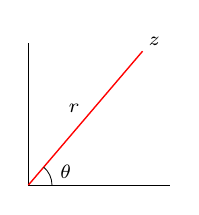
\begin{tikzpicture}[scale=.5]
  \draw[line width=.3pt] (0,3.6)--(0,0)--(3.6,0);
  \draw[red,line width=.5pt] (0,0)--node[above left=-2pt,font=\scriptsize,black]{$r$}
    (2.9,3.4) node[above right=-2pt,font=\scriptsize,black]{$z$};
  \draw[line width=.3pt] (.6,0) arc (0:49.5:.6);
  \node[font=\scriptsize] at (.95,.35) {$\theta$};
\end{tikzpicture}}{Representation of a complex number with polar coordinates.}%
For the proof below, we need to know that every $z\in\C$ has a square root in
$\C$. To show this, write
\[ z = r(\cos\theta + i\sin\theta), \]
where $r$ is the length of the line segment in the complex plane from the origin
to $z$ and $\theta$ is the angle of that line segment with the positive
horizontal axis. Then
\[ \sqrt{r}\Bigl(\cos\tfrac{\theta}{2} + i\sin\tfrac{\theta}{2}\Bigr) \]
is a square root of $z$, as you can verify by showing that the square of the
complex number above equals $z$.

\begin{result}[Over $\C$, invertible operators have square roots]\label{ax:8.41}
Suppose $V$ is a complex vector space and $T\in\Lin(V)$ is invertible. Then $T$
has a square root.
\end{result}

\begin{proof}
Let $\lambda_1,\dots,\lambda_m$ be the distinct eigenvalues of $T$. For each
$k$, there exists a nilpotent operator $T_k\in\Lin\bigl(G(\lambda_k,T)\bigr)$
such that $T|_{G(\lambda_k,T)}=\lambda_kI+T_k$ [see \ref{ax:8.22}(b)]. Because
$T$ is invertible, none of the $\lambda_k$'s equals $0$, so we can write
\[ T|_{G(\lambda_k,T)} = \lambda_k\Bigl(I+\frac{T_k}{\lambda_k}\Bigr) \]
for each $k$. Because $T_k/\lambda_k$ is nilpotent, $I+T_k/\lambda_k$ has a
square root (by \ref{ax:8.39}). Multiplying a square root of the complex number
$\lambda_k$ by a square root of $I+T_k/\lambda_k$, we obtain a square root
$R_k$ of $T|_{G(\lambda_k,T)}$.

By the generalized eigenspace decomposition (\ref{ax:8.22}), a typical vector
$v\in V$ can be written uniquely in the form
\[ v = u_1+\cdots+u_m, \]
where each $u_k$ is in $G(\lambda_k,T)$. Using this decomposition, define an
operator $R\in\Lin(V)$ by
\[ Rv = R_1u_1+\cdots+R_mu_m. \]
You should verify that this operator $R$ is a square root of $T$, completing the
proof.
\end{proof}

By imitating the techniques in this subsection, you should be able to prove that
if $V$ is a complex vector space and $T\in\Lin(V)$ is invertible, then $T$ has a
$k^{\text{th}}$ root for every positive integer $k$.

\subsection{Jordan Form}

We know that if $V$ is a complex vector space, then for every $T\in\Lin(V)$
there is a basis of $V$ with respect to which $T$ has a nice upper-triangular
matrix (see \ref{ax:8.37}). In this subsection we will see that we can do even
better---there is a basis of $V$ with respect to which the matrix of $T$
contains $0$'s everywhere except possibly on the diagonal and the line directly
above the diagonal.

We begin by looking at two examples of nilpotent operators.

\begin{example}[Nilpotent operator with nice matrix]\label{ax:8.42}
Let $T$ be the operator on $\C^4$ defined by
\[ T(z_1,z_2,z_3,z_4) = (0,z_1,z_2,z_3). \]
Then $T^4=0$; thus $T$ is nilpotent. If $v=(1,0,0,0)$, then $T^3v,T^2v,Tv,v$ is
a basis of $\C^4$. The matrix of $T$ with respect to this basis is
\[ \begin{pmatrix}
0&1&0&0\\
0&0&1&0\\
0&0&0&1\\
0&0&0&0
\end{pmatrix}. \]
\end{example}

The next example of a nilpotent operator has more complicated behavior than the
example above.

\begin{example}[Nilpotent operator with slightly more complicated matrix]\label{ax:8.43}
Let $T$ be the operator on $\C^6$ defined by
\[ T(z_1,z_2,z_3,z_4,z_5,z_6) = (0,z_1,z_2,0,z_4,0). \]
Then $T^3=0$; thus $T$ is nilpotent. In contrast to the nice behavior of the
nilpotent operator of the previous example, for this nilpotent operator there
does not exist a vector $v\in\C^6$ such that $T^5v,T^4v,T^3v,T^2v,Tv,v$ is a
basis of $\C^6$. However, if we take $v_1=(1,0,0,0,0,0)$, $v_2=(0,0,0,1,0,0)$,
and $v_3=(0,0,0,0,0,1)$, then $T^2v_1,Tv_1,v_1,Tv_2,v_2,v_3$ is a basis of
$\C^6$. The matrix of $T$ with respect to this basis is
\[ \begin{pmatrix}
\begin{pmatrix}0&1&0\\0&0&1\\0&0&0\end{pmatrix}
  & \begin{matrix}0&0\\0&0\\0&0\end{matrix}
  & \begin{matrix}0\\0\\0\end{matrix}\\
\begin{matrix}0&0&0\\0&0&0\end{matrix}
  & \begin{pmatrix}0&1\\0&0\end{pmatrix}
  & \begin{matrix}0\\0\end{matrix}\\
\begin{matrix}0&0&0\end{matrix}
  & \begin{matrix}0&0\end{matrix}
  & \begin{pmatrix}0\end{pmatrix}
\end{pmatrix}. \]
Here the inner matrices are blocked off to show that we can think of the
6-by-6 matrix above as a block diagonal matrix consisting of a 3-by-3 block
with $1$'s on the line above the diagonal and $0$'s elsewhere, a 2-by-2 block
with $1$ above the diagonal and $0$'s elsewhere, and a 1-by-1 block
containing~$0$.
\end{example}

Our next goal is to show that every nilpotent operator $T\in\Lin(V)$ behaves
similarly to the operator in the previous example. Specifically, there is a
finite collection of vectors $v_1,\dots,v_n\in V$ such that there is a basis of
$V$ consisting of the vectors of the form $T^jv_k$, as $k$ varies from $1$ to
$n$ and $j$ varies (in reverse order) from $0$ to the largest nonnegative
integer $m_k$ such that $T^{m_k}v_k\ne0$. With respect to this basis, the matrix
of $T$ looks like the matrix in the previous example. More specifically, $T$
has a block diagonal matrix with respect to this basis, with each block a
square matrix that is $0$ everywhere except on the line above the diagonal.

In the next definition, the diagonal of each $A_k$ is filled with some
eigenvalue $\lambda_k$ of $T$, the line directly above the diagonal of $A_k$ is
filled with $1$'s, and all other entries in $A_k$ are $0$ (to understand why
each $\lambda_k$ is an eigenvalue of $T$, see \ref{ax:5.41}). The
$\lambda_k$'s need not be distinct. Also, $A_k$ may be a 1-by-1 matrix
$(\lambda_k)$ containing just an eigenvalue of $T$. If each $\lambda_k$ is $0$,
then the next definition captures the behavior described in the paragraph above
(recall that if $T$ is nilpotent, then $0$ is the only eigenvalue of $T$).

\begin{definition}[Jordan basis]\label{ax:8.44}
Suppose $T\in\Lin(V)$. A basis of $V$ is called a \emph{Jordan basis} for $T$
if with respect to this basis $T$ has a block diagonal matrix
\[ \begin{pmatrix}
A_1 & & 0\\
& \ddots & \\
0 & & A_p
\end{pmatrix} \]
in which each $A_k$ is an upper-triangular matrix of the form
\[ A_k = \begin{pmatrix}
\lambda_k & 1 & & 0\\
& \ddots & \ddots & \\
& & \ddots & 1\\
0 & & & \lambda_k
\end{pmatrix}. \]
\end{definition}

Most of the work in proving that every operator on a finite-dimensional complex
vector space has a Jordan basis occurs in proving the special case below of
nilpotent operators. This special case holds on real vector spaces as well as
complex vector spaces.

\begin{result}[Every nilpotent operator has a Jordan basis]\label{ax:8.45}
Suppose $T\in\Lin(V)$ is nilpotent. Then there is a basis of $V$ that is a
Jordan basis for $T$.
\end{result}

\begin{proof}
We will prove this result by induction on $\dim V$. To get started, note that
the desired result holds if $\dim V=1$ (because in that case, the only nilpotent
operator is the $0$ operator). Now assume that $\dim V>1$ and that the desired
result holds on all vector spaces of smaller dimension.

Let $m$ be the smallest positive integer such that $T^m=0$. Thus there exists
$u\in V$ such that $T^{m-1}u\ne0$. Let
\[ U = \spn(u,Tu,\dots,T^{m-1}u). \]
The list $u,Tu,\dots,T^{m-1}u$ is linearly independent (see Exercise~2 in
Section~8A). If $U=V$, then writing this list in reverse order gives a Jordan
basis for $T$ and we are done. Thus we can assume that $U\ne V$.

Note that $U$ is invariant under $T$. By our induction hypothesis, there is a
basis of $U$ that is a Jordan basis for $T|_U$. The strategy of our proof is
that we will find a subspace $W$ of $V$ such that $W$ is also invariant under
$T$ and $V=U\oplus W$. Again by our induction hypothesis, there will be a basis
of $W$ that is a Jordan basis for $T|_W$. Putting together the Jordan bases for
$T|_U$ and $T|_W$, we will have a Jordan basis for $T$.

Let $\varphi\in V'$ be such that $\varphi(T^{m-1}u)\ne0$. Let
\[ W = \bigl\{v\in V : \varphi(T^kv)=0 \text{ for each } k=0,\dots,m-1\bigr\}. \]
Then $W$ is a subspace of $V$ that is invariant under $T$ $\bigl($the invariance
holds because if $v\in W$ then $\varphi\bigl(T^k(Tv)\bigr)=0$ for
$k=0,\dots,m-1$, where the case $k=m-1$ holds because $T^m=0\bigr)$. We will
show that $V=U\oplus W$, which by the previous paragraph will complete the
proof.

To show that $U+W$ is a direct sum, suppose $v\in U\cap W$ with $v\ne0$.
Because $v\in U$, there exist $c_0,\dots,c_{m-1}\in\F$ such that
\[ v = c_0u + c_1Tu + \cdots + c_{m-1}T^{m-1}u. \]
Let $j$ be the smallest index such that $c_j\ne0$. Apply $T^{m-j-1}$ to both
sides of the equation above, getting
\[ T^{m-j-1}v = c_jT^{m-1}u, \]
where we have used the equation $T^m=0$. Now apply $\varphi$ to both sides of
the equation above, getting
\[ \varphi(T^{m-j-1}v) = c_j\varphi(T^{m-1}u) \ne 0. \]
The equation above shows that $v\notin W$. Hence we have proved that
$U\cap W=\{0\}$, which implies that $U+W$ is a direct sum (see
\ref{ax:1.46}).

To show that $U\oplus W=V$, define $S\colon V\to\F^m$ by
\[ Sv = \bigl(\varphi(v),\varphi(Tv),\dots,\varphi(T^{m-1}v)\bigr). \]
Thus $\nul S=W$. Hence
\[ \dim W = \dim\nul S = \dim V - \dim\range S \ge \dim V - m, \]
where the second equality comes from the fundamental theorem of linear maps
(\ref{ax:3.21}). Using the inequality above, we have
\[ \dim(U\oplus W) = \dim U + \dim W \ge m + (\dim V - m) = \dim V. \]
Thus $U\oplus W=V$ (by \ref{ax:2.39}), completing the proof.
\end{proof}

\marginnote{Camille Jordan (1838--1922) published a proof of \ref{ax:8.46} in
1870.}%
Now the generalized eigenspace decomposition allows us to extend the previous
result to operators that may not be nilpotent. Doing this requires that we deal
with complex vector spaces.

\begin{result}[Jordan form]\label{ax:8.46}
Suppose $\F=\C$ and $T\in\Lin(V)$. Then there is a basis of $V$ that is a
Jordan basis for $T$.
\end{result}

\begin{proof}
Let $\lambda_1,\dots,\lambda_m$ be the distinct eigenvalues of $T$. The
generalized eigenspace decomposition states that
\[ V = G(\lambda_1,T)\oplus\cdots\oplus G(\lambda_m,T), \]
where each $(T-\lambda_kI)|_{G(\lambda_k,T)}$ is nilpotent (see
\ref{ax:8.22}). Thus \ref{ax:8.45} implies that some basis of each
$G(\lambda_k,T)$ is a Jordan basis for $(T-\lambda_kI)|_{G(\lambda_k,T)}$. Put
these bases together to get a basis of $V$ that is a Jordan basis for $T$.
\end{proof}

% ------------------------------------------------------------------ exercises
\exercisesheading{8C}

\begin{exercise}
Suppose $T\in\Lin(\C^3)$ is the operator defined by
$T(z_1,z_2,z_3)=(z_2,z_3,0)$. Prove that $T$ does not have a square root.
\end{exercise}

\begin{exercise}
Define $T\in\Lin(\F^5)$ by
$T(x_1,x_2,x_3,x_4,x_5)=(2x_2,3x_3,-x_4,4x_5,0)$.
\begin{parts}
\item Show that $T$ is nilpotent.
\item Find a square root of $I+T$.
\end{parts}
\end{exercise}

\begin{exercise}
Suppose $V$ is a complex vector space. Prove that every invertible operator on
$V$ has a cube root.
\end{exercise}

\begin{exercise}
Suppose $V$ is a real vector space. Prove that the operator $-I$ on $V$ has a
square root if and only if $\dim V$ is an even number.
\end{exercise}

\begin{exercise}
Suppose $T\in\Lin(\C^2)$ is the operator defined by $T(w,z)=(-w-z,9w+5z)$.
Find a Jordan basis for $T$.
\end{exercise}

\begin{exercise}
Find a basis of $\Poly_4(\R)$ that is a Jordan basis for the differentiation
operator $D$ on $\Poly_4(\R)$ defined by $Dp=p'$.
\end{exercise}

\begin{exercise}
Suppose $T\in\Lin(V)$ is nilpotent and $v_1,\dots,v_n$ is a Jordan basis for
$T$. Prove that the minimal polynomial of $T$ is $z^{m+1}$, where $m$ is the
length of the longest consecutive string of $1$'s that appears on the line
directly above the diagonal in the matrix of $T$ with respect to
$v_1,\dots,v_n$.
\end{exercise}

\begin{exercise}
Suppose $T\in\Lin(V)$ and $v_1,\dots,v_n$ is a basis of $V$ that is a Jordan
basis for $T$. Describe the matrix of $T^2$ with respect to this basis.
\end{exercise}

\begin{exercise}
Suppose $T\in\Lin(V)$ is nilpotent. Explain why there exist
$v_1,\dots,v_n\in V$ and nonnegative integers $m_1,\dots,m_n$ such that (a)
and (b) below both hold.
\begin{parts}
\item $T^{m_1}v_1,\dots,Tv_1,v_1,\dots,T^{m_n}v_n,\dots,Tv_n,v_n$ is a basis
  of $V$.
\item $T^{m_1+1}v_1=\cdots=T^{m_n+1}v_n=0$.
\end{parts}
\end{exercise}

\begin{exercise}
Suppose $T\in\Lin(V)$ and $v_1,\dots,v_n$ is a basis of $V$ that is a Jordan
basis for $T$. Describe the matrix of $T$ with respect to the basis
$v_n,\dots,v_1$ obtained by reversing the order of the $v$'s.
\end{exercise}

\begin{exercise}
Suppose $T\in\Lin(V)$. Explain why every vector in each Jordan basis for $T$ is
a generalized eigenvector of $T$.
\end{exercise}

\begin{exercise}
Suppose $T\in\Lin(V)$ is diagonalizable. Show that $\Mat(T)$ is a diagonal
matrix with respect to every Jordan basis for $T$.
\end{exercise}

\begin{exercise}
Suppose $T\in\Lin(V)$ is nilpotent. Prove that if $v_1,\dots,v_n$ are vectors
in $V$ and $m_1,\dots,m_n$ are nonnegative integers such that
\[ T^{m_1}v_1,\dots,Tv_1,v_1,\dots,T^{m_n}v_n,\dots,Tv_n,v_n \text{ is a basis
of } V \]
and
\[ T^{m_1+1}v_1=\cdots=T^{m_n+1}v_n=0, \]
then $T^{m_1}v_1,\dots,T^{m_n}v_n$ is a basis of $\nul T$.
\exnote{This exercise shows that $n=\dim\nul T$. Thus the positive integer $n$
that appears above depends only on $T$ and not on the specific Jordan basis
chosen for $T$.}
\end{exercise}

\begin{exercise}
Suppose $\F=\C$ and $T\in\Lin(V)$. Prove that there does not exist a direct sum
decomposition of $V$ into two nonzero subspaces invariant under $T$ if and only
if the minimal polynomial of $T$ is of the form $(z-\lambda)^{\dim V}$ for some
$\lambda\in\C$.
\end{exercise}

% Source: book pp. 326--331 (PDF 340--345).
\section{Trace: A Connection Between Matrices and Operators}

We begin this section by defining the trace of a square matrix. After
developing some properties of the trace of a square matrix, we will use this
concept to define the trace of an operator.

\begin{definition}[Trace of a matrix]\label{ax:8.47}
Suppose $A$ is a square matrix with entries in $\F$. The \emph{trace} of $A$,
denoted $\tr A$, is defined to be the sum of the diagonal entries of $A$.
\end{definition}

\begin{example}[Trace of a 3-by-3 matrix]\label{ax:8.48}
Suppose
\[ A = \begin{pmatrix}
{\color{red}3} & -1 & -2\\
5 & {\color{red}2} & -3\\
1 & 6 & {\color{red}0}
\end{pmatrix}. \]
The diagonal entries of $A$, which are shown in red above, are $3$, $2$, and
$0$. Thus $\tr A=3+2+0=5$.
\end{example}

Matrix multiplication is not commutative, but the next result shows that the
order of matrix multiplication does not matter to the trace.

\begin{result}[Trace of $AB$ equals trace of $BA$]\label{ax:8.49}
Suppose $A$ is an $m$-by-$n$ matrix and $B$ is an $n$-by-$m$ matrix. Then
\[ \tr(AB) = \tr(BA). \]
\end{result}

\begin{proof}
Suppose
\[ A = \begin{pmatrix}
A_{1,1} & \cdots & A_{1,n}\\
\vdots & & \vdots\\
A_{m,1} & \cdots & A_{m,n}
\end{pmatrix}, \quad
B = \begin{pmatrix}
B_{1,1} & \cdots & B_{1,m}\\
\vdots & & \vdots\\
B_{n,1} & \cdots & B_{n,m}
\end{pmatrix}. \]
The $j^{\text{th}}$ term on the diagonal of the $m$-by-$m$ matrix $AB$ equals
$\sum_{k=1}^n A_{j,k}B_{k,j}$. Thus
\begin{align*}
\tr(AB) &= \sum_{j=1}^m \sum_{k=1}^n A_{j,k}B_{k,j}\\
&= \sum_{k=1}^n \sum_{j=1}^m B_{k,j}A_{j,k}\\
&= \sum_{k=1}^n (k^{\text{th}} \text{ term on diagonal of the
  $n$-by-$n$ matrix } BA)\\
&= \tr(BA),
\end{align*}
as desired.
\end{proof}

We want to define the trace of an operator $T\in\Lin(V)$ to be the trace of the
matrix of $T$ with respect to some basis of $V$. However, this definition should
not depend on the choice of basis. The following result will make this
possible.

\begin{result}[Trace of matrix of operator does not depend on basis]\label{ax:8.50}
Suppose $T\in\Lin(V)$. Suppose $u_1,\dots,u_n$ and $v_1,\dots,v_n$ are bases
of $V$. Then
\[ \tr\Mat\bigl(T,(u_1,\dots,u_n)\bigr) = \tr\Mat\bigl(T,(v_1,\dots,v_n)\bigr). \]
\end{result}

\begin{proof}
Let $A=\Mat\bigl(T,(u_1,\dots,u_n)\bigr)$ and
$B=\Mat\bigl(T,(v_1,\dots,v_n)\bigr)$. The change-of-basis formula tells us
that there exists an invertible $n$-by-$n$ matrix $C$ such that $A=C^{-1}BC$
(see \ref{ax:3.84}). Thus
\begin{align*}
\tr A &= \tr\bigl((C^{-1}B)C\bigr)\\
&= \tr\bigl(C(C^{-1}B)\bigr)\\
&= \tr\bigl((CC^{-1})B\bigr)\\
&= \tr B,
\end{align*}
where the second line comes from \ref{ax:8.49}.
\end{proof}

Because of \ref{ax:8.50}, the following definition now makes sense.

\begin{definition}[Trace of an operator]\label{ax:8.51}
Suppose $T\in\Lin(V)$. The \emph{trace} of $T$, denoted $\tr T$, is defined by
\[ \tr T = \tr\Mat\bigl(T,(v_1,\dots,v_n)\bigr), \]
where $v_1,\dots,v_n$ is any basis of $V$.
\end{definition}

Suppose $T\in\Lin(V)$ and $\lambda$ is an eigenvalue of $T$. Recall that we
defined the multiplicity of $\lambda$ to be the dimension of the generalized
eigenspace $G(\lambda,T)$ (see \ref{ax:8.23}); we proved that this multiplicity
equals $\dim\nul(T-\lambda I)^{\dim V}$ (see \ref{ax:8.20}). Recall also that
if $V$ is a complex vector space, then the sum of the multiplicities of all
eigenvalues of $T$ equals $\dim V$ (see \ref{ax:8.25}).

In the following result, the sum of the eigenvalues ``with each eigenvalue
included as many times as its multiplicity'' means that if
$\lambda_1,\dots,\lambda_m$ are the distinct eigenvalues of $T$ with
multiplicities $d_1,\dots,d_m$, then the sum is
\[ d_1\lambda_1+\cdots+d_m\lambda_m. \]
Or if you prefer to work with a list of not-necessarily-distinct eigenvalues,
with each eigenvalue included as many times as its multiplicity, then the
eigenvalues could be denoted by $\lambda_1,\dots,\lambda_n$ (where $n$ equals
$\dim V$) and the sum is
\[ \lambda_1+\cdots+\lambda_n. \]

\begin{result}[On complex vector spaces, trace equals sum of eigenvalues]\label{ax:8.52}
Suppose $\F=\C$ and $T\in\Lin(V)$. Then $\tr T$ equals the sum of the
eigenvalues of $T$, with each eigenvalue included as many times as its
multiplicity.
\end{result}

\begin{proof}
There is a basis of $V$ with respect to which $T$ has an upper-triangular matrix
with the diagonal entries of the matrix consisting of the eigenvalues of $T$,
with each eigenvalue included as many times as its multiplicity---see
\ref{ax:8.37}. Thus the definition of the trace of an operator along with
\ref{ax:8.50}, which allows us to use a basis of our choice, implies that
$\tr T$ equals the sum of the eigenvalues of $T$, with each eigenvalue included
as many times as its multiplicity.
\end{proof}

\begin{example}[Trace of an operator on $\C^3$]\label{ax:8.53}
Suppose $T\in\Lin(\C^3)$ is defined by
\[ T(z_1,z_2,z_3) = (3z_1-z_2-2z_3,\,3z_1+2z_2-3z_3,\,z_1+2z_2). \]
Then the matrix of $T$ with respect to the standard basis of $\C^3$ is
\[ \begin{pmatrix}
3 & -1 & -2\\
3 & 2 & -3\\
1 & 2 & 0
\end{pmatrix}. \]
Adding up the diagonal entries of this matrix, we see that $\tr T=5$.

The eigenvalues of $T$ are $1$, $2+3i$, and $2-3i$, each with multiplicity
$1$, as you can verify. The sum of these eigenvalues, each included as many
times as its multiplicity, is $1+(2+3i)+(2-3i)$, which equals $5$, as expected
by \ref{ax:8.52}.
\end{example}

The trace has a close connection with the characteristic polynomial. Suppose
$\F=\C$, $T\in\Lin(V)$, and $\lambda_1,\dots,\lambda_n$ are the eigenvalues of
$T$, with each eigenvalue included as many times as its multiplicity. Then by
definition (see \ref{ax:8.26}), the characteristic polynomial of $T$ equals
\[ (z-\lambda_1)\cdots(z-\lambda_n). \]
Expanding the polynomial above, we can write the characteristic polynomial of
$T$ in the form
\[ z^n - (\lambda_1+\cdots+\lambda_n)z^{n-1} + \cdots
   + (-1)^n(\lambda_1\cdots\lambda_n). \]

The expression above immediately leads to the next result. Also see
\ref{ax:9.65}, which does not require the hypothesis that $\F=\C$.

\begin{result}[Trace and characteristic polynomial]\label{ax:8.54}
Suppose $\F=\C$ and $T\in\Lin(V)$. Let $n=\dim V$. Then $\tr T$ equals the
negative of the coefficient of $z^{n-1}$ in the characteristic polynomial of
$T$.
\end{result}

The next result gives a nice formula for the trace of an operator on an inner
product space.

\begin{result}[Trace on an inner product space]\label{ax:8.55}
Suppose $V$ is an inner product space, $T\in\Lin(V)$, and $e_1,\dots,e_n$ is an
orthonormal basis of $V$. Then
\[ \tr T = \ip{Te_1}{e_1} + \cdots + \ip{Te_n}{e_n}. \]
\end{result}

\begin{proof}
The desired formula follows from the observation that the entry in row $k$,
column $k$ of $\Mat\bigl(T,(e_1,\dots,e_n)\bigr)$ equals $\ip{Te_k}{e_k}$
[use \ref{ax:6.30}(a) with $v=Te_k$].
\end{proof}

The algebraic properties of the trace as defined on square matrices translate
to algebraic properties of the trace as defined on operators, as shown in the
next result.

\begin{result}[Trace is linear]\label{ax:8.56}
The function $\tr\colon\Lin(V)\to\F$ is a linear functional on $\Lin(V)$ such
that
\[ \tr(ST) = \tr(TS) \]
for all $S,T\in\Lin(V)$.
\end{result}

\begin{proof}
Choose a basis of $V$. All matrices of operators in this proof will be with
respect to that basis. Suppose $S,T\in\Lin(V)$.

If $\lambda\in\F$, then
\[ \tr(\lambda T) = \tr\Mat(\lambda T) = \tr\bigl(\lambda\Mat(T)\bigr)
   = \lambda\tr\Mat(T) = \lambda\tr T, \]
where the first and last equalities come from the definition of the trace of an
operator, the second equality comes from \ref{ax:3.38}, and the third equality
follows from the definition of the trace of a square matrix.

Also,
\[ \tr(S+T) = \tr\Mat(S+T) = \tr\bigl(\Mat(S)+\Mat(T)\bigr)
   = \tr\Mat(S) + \tr\Mat(T) = \tr S + \tr T, \]
where the first and last equalities come from the definition of the trace of an
operator, the second equality comes from \ref{ax:3.35}, and the third equality
follows from the definition of the trace of a square matrix. The two paragraphs
above show that $\tr\colon\Lin(V)\to\F$ is a linear functional on $\Lin(V)$.

Furthermore,
\begin{multline*}
\tr(ST) = \tr\Mat(ST) = \tr\bigl(\Mat(S)\Mat(T)\bigr)\\
= \tr\bigl(\Mat(T)\Mat(S)\bigr) = \tr\Mat(TS) = \tr(TS),
\end{multline*}
where the second and fourth equalities come from \ref{ax:3.43} and the crucial
third equality comes from \ref{ax:8.49}.
\end{proof}

The equations $\tr(ST)=\tr(TS)$ and $\tr I=\dim V$ uniquely characterize the
trace among the linear functionals on $\Lin(V)$---see Exercise~10.

\marginnote{The statement of the next result does not involve traces, but the
short proof uses traces. When something like this happens in mathematics, then
usually a good definition lurks in the background.}%
The equation $\tr(ST)=\tr(TS)$ leads to our next result, which does not hold on
infinite-dimensional vector spaces (see Exercise~13). However, additional
hypotheses on $S$, $T$, and $V$ lead to an infinite-dimensional generalization
of the result below, with important applications to quantum theory.

\begin{result}[Identity operator is not the difference of $ST$ and $TS$]\label{ax:8.57}
There do not exist operators $S,T\in\Lin(V)$ such that $ST-TS=I$.
\end{result}

\begin{proof}
Suppose $S,T\in\Lin(V)$. Then
\[ \tr(ST-TS) = \tr(ST) - \tr(TS) = 0, \]
where both equalities come from \ref{ax:8.56}. The trace of $I$ equals
$\dim V$, which is not $0$. Because $ST-TS$ and $I$ have different traces, they
cannot be equal.
\end{proof}

% ------------------------------------------------------------------ exercises
\exercisesheading{8D}

\begin{exercise}
Suppose $V$ is an inner product space and $v,w\in V$. Define an operator
$T\in\Lin(V)$ by $Tu=\ip{u}{v}w$. Find a formula for $\tr T$.
\end{exercise}

\begin{exercise}
Suppose $P\in\Lin(V)$ satisfies $P^2=P$. Prove that
\[ \tr P = \dim\range P. \]
\end{exercise}

\begin{exercise}
Suppose $T\in\Lin(V)$ and $T^5=T$. Prove that the real and imaginary parts of
$\tr T$ are both integers.
\end{exercise}

\begin{exercise}
Suppose $V$ is an inner product space and $T\in\Lin(V)$. Prove that
\[ \tr T^* = \overline{\tr T}. \]
\end{exercise}

\begin{exercise}
Suppose $V$ is an inner product space. Suppose $T\in\Lin(V)$ is a positive
operator and $\tr T=0$. Prove that $T=0$.
\end{exercise}

\begin{exercise}
Suppose $V$ is an inner product space and $P,Q\in\Lin(V)$ are orthogonal
projections. Prove that $\tr(PQ)\ge0$.
\end{exercise}

\begin{exercise}
Suppose $T\in\Lin(\C^3)$ is the operator whose matrix is
\[ \begin{pmatrix}
51 & -12 & -21\\
60 & -40 & -28\\
57 & -68 & 1
\end{pmatrix}. \]
Someone tells you (accurately) that $-48$ and $24$ are eigenvalues of $T$.
Without using a computer or writing anything down, find the third eigenvalue
of $T$.
\end{exercise}

\begin{exercise}
Prove or give a counterexample: If $S,T\in\Lin(V)$, then
$\tr(ST)=(\tr S)(\tr T)$.
\end{exercise}

\begin{exercise}
Suppose $T\in\Lin(V)$ is such that $\tr(ST)=0$ for all $S\in\Lin(V)$. Prove
that $T=0$.
\end{exercise}

\begin{exercise}
Prove that the trace is the only linear functional $\tau\colon\Lin(V)\to\F$
such that
\[ \tau(ST) = \tau(TS) \]
for all $S,T\in\Lin(V)$ and $\tau(I)=\dim V$.
\exnote{Hint: Suppose that $v_1,\dots,v_n$ is a basis of $V$. For
$j,k\in\{1,\dots,n\}$, define $P_{j,k}\in\Lin(V)$ by
$P_{j,k}(a_1v_1+\cdots+a_nv_n)=a_kv_j$. Prove that
\[ \tau(P_{j,k}) = \begin{cases} 1 & \text{if } j=k,\\
   0 & \text{if } j\ne k. \end{cases} \]
Then for $T\in\Lin(V)$, use the equation
$T=\sum_{k=1}^n\sum_{j=1}^n\Mat(T)_{j,k}P_{j,k}$ to show that $\tau(T)=\tr T$.}
\end{exercise}

\begin{exercise}
Suppose $V$ and $W$ are inner product spaces and $T\in\Lin(V,W)$. Prove that if
$e_1,\dots,e_n$ is an orthonormal basis of $V$ and $f_1,\dots,f_m$ is an
orthonormal basis of $W$, then
\[ \tr(T^*T) = \sum_{k=1}^n\sum_{j=1}^m \abs{\ip{Te_k}{f_j}}^2. \]
\exnote{The numbers $\ip{Te_k}{f_j}$ are the entries of the matrix of $T$ with
respect to the orthonormal bases $e_1,\dots,e_n$ and $f_1,\dots,f_m$. These
numbers depend on the bases, but $\tr(T^*T)$ does not depend on a choice of
bases. Thus this exercise shows that the sum of the squares of the absolute
values of the matrix entries does not depend on which orthonormal bases are
used.}
\end{exercise}

\begin{exercise}
Suppose $V$ and $W$ are finite-dimensional inner product spaces.
\begin{parts}
\item Prove that $\ip{S}{T}=\tr(T^*S)$ defines an inner product on
  $\Lin(V,W)$.
\item Suppose $e_1,\dots,e_n$ is an orthonormal basis of $V$ and
  $f_1,\dots,f_m$ is an orthonormal basis of $W$. Show that the inner product
  on $\Lin(V,W)$ from (a) is the same as the standard inner product on
  $\F^{mn}$, where we identify each element of $\Lin(V,W)$ with its matrix
  (with respect to the bases just mentioned) and then with an element of
  $\F^{mn}$.
\end{parts}
\exnote{Caution: The norm of a linear map $T\in\Lin(V,W)$ as defined by
\ref{ax:7.86} is not the same as the norm that comes from the inner product in
(a) above. Unless explicitly stated otherwise, always assume that $\norm{T}$
refers to the norm as defined by \ref{ax:7.86}. The norm that comes from the
inner product in (a) is called the \textbf{Frobenius norm} or the
\textbf{Hilbert--Schmidt norm}.}
\end{exercise}

\begin{exercise}
Find $S,T\in\Lin\bigl(\Poly(\F)\bigr)$ such that $ST-TS=I$.
\exnote{Hint: Make an appropriate modification of the operators in
Example~\ref{ax:3.9}.}
\exnote{This exercise shows that additional hypotheses are needed on $S$ and $T$
to extend \ref{ax:8.57} to the setting of infinite-dimensional vector spaces.}
\end{exercise}


% Chapter 9: assembled from chapters/ch09/*.tex
% Source: book p. 332 (PDF 346).
\chapter{Multilinear Algebra and Determinants}

We begin this chapter by investigating bilinear forms and quadratic forms on a
vector space. Then we will move on to multilinear forms. We will show that the
vector space of alternating $n$-linear forms has dimension one on a vector space
of dimension $n$. This result will allow us to give a clean basis-free
definition of the determinant of an operator.

{\emergencystretch=1.5em
This approach to the determinant via alternating multilinear forms leads to
straightforward proofs of key properties of determinants. For example, we will
see that the determinant is multiplicative, meaning that
$\det(ST)=(\det S)(\det T)$ for all operators $S$ and $T$ on the same vector
space. We will also see that $T$ is invertible if and only if $\det T\ne0$.
Another important result states that the determinant of an operator on a
complex vector space equals the product of the eigenvalues of the operator,
with each eigenvalue included as many times as its multiplicity.\par}

The chapter concludes with an introduction to tensor products.

\begin{definition*}[Standing assumptions for this chapter]\leavevmode
\begin{itemize}
\item $\F$ denotes $\R$ or $\C$.
\item $V$ and $W$ denote finite-dimensional nonzero vector spaces over $\F$.
\end{itemize}
\end{definition*}

% Source: book pp. 333--345 (PDF 347--359); no solutions.
% \exnote: Axler's small italic comment under an exercise
\section{Bilinear Forms and Quadratic Forms}

\subsection{Bilinear Forms}

A bilinear form on $V$ is a function from $V\times V$ to $\F$ that is linear in
each slot separately, meaning that if we hold either slot fixed then we have a
linear function in the other slot. Here is the formal definition.

\begin{definition}[Bilinear form]\label{ax:9.1}
A \emph{bilinear form} on $V$ is a function $\beta\colon V\times V\to\F$ such
that
\[ v\mapsto\beta(v,u) \quad\text{and}\quad v\mapsto\beta(u,v) \]
are both linear functionals on $V$ for every $u\in V$.
\end{definition}

\marginnote{Recall that the term \textbf{linear functional}, used in the
definition above, means a linear function that maps into the scalar field $\F$.
Thus the term \textbf{bilinear functional} would be more consistent terminology
than \textbf{bilinear form}, which unfortunately has become standard.}%
For example, if $V$ is a real inner product space, then the function that takes
an ordered pair $(u,v)\in V\times V$ to $\ip{u}{v}$ is a bilinear form on $V$.
If $V$ is a nonzero complex inner product space, then this function is not a
bilinear form because the inner product is not linear in the second slot
(complex scalars come out of the second slot as their complex conjugates).

If $\F=\R$, then a bilinear form differs from an inner product in that an inner
product requires symmetry $\bigl[$meaning that $\beta(v,w)=\beta(w,v)$ for all
$v,w\in V\bigr]$ and positive definiteness $\bigl[$meaning that
$\beta(v,v)>0$ for all $v\in V\setminus\{0\}\bigr]$, but these properties are
not required for a bilinear form.

\begin{example}[Bilinear forms]\label{ax:9.2}\emergencystretch=1.5em\leavevmode
\begin{itemize}
\item The function $\beta\colon\F^3\times\F^3\to\F$ defined by
  \[ \beta\bigl((x_1,x_2,x_3),(y_1,y_2,y_3)\bigr)
     = x_1y_2-5x_2y_3+2x_3y_1 \]
  is a bilinear form on $\F^3$.
\item Suppose $A$ is an $n$-by-$n$ matrix with $A_{j,k}\in\F$ in row $j$,
  column $k$. Define a bilinear form $\beta_A$ on $\F^n$ by
  \[ \beta_A\bigl((x_1,\dots,x_n),(y_1,\dots,y_n)\bigr)
     = \sum_{k=1}^n\sum_{j=1}^n A_{j,k}x_jy_k. \]
  The first bullet point is a special case of this bullet point with $n=3$ and
  \[ A = \begin{pmatrix} 0&1&0\\ 0&0&-5\\ 2&0&0 \end{pmatrix}. \]
\item Suppose $V$ is a real inner product space and $T\in\Lin(V)$. Then the
  function $\beta\colon V\times V\to\R$ defined by
  \[ \beta(u,v) = \ip{u}{Tv} \]
  is a bilinear form on $V$.
\item If $n$ is a positive integer, then the function
  $\beta\colon\Poly_n(\R)\times\Poly_n(\R)\to\R$ defined by
  \[ \beta(p,q) = p(2)\cdot q'(3) \]
  is a bilinear form on $\Poly_n(\R)$.
\item Suppose $\varphi,\tau\in V'$. Then the function
  $\beta\colon V\times V\to\F$ defined by
  \[ \beta(u,v) = \varphi(u)\cdot\tau(v) \]
  is a bilinear form on $V$.
\item More generally, suppose that
  $\varphi_1,\dots,\varphi_n,\tau_1,\dots,\tau_n\in V'$. Then the function
  $\beta\colon V\times V\to\F$ defined by
  \[ \beta(u,v) = \varphi_1(u)\cdot\tau_1(v)+\cdots+\varphi_n(u)\cdot\tau_n(v) \]
  is a bilinear form on $V$.
\end{itemize}
\end{example}

A bilinear form on $V$ is a function from $V\times V$ to $\F$. Because
$V\times V$ is a vector space, this raises the question of whether a bilinear
form can also be a linear map from $V\times V$ to $\F$. Note that none of the
bilinear forms in \ref{ax:9.2} are linear maps except in some special cases in
which the bilinear form is the zero map. Exercise~3 shows that a bilinear form
$\beta$ on $V$ is a linear map on $V\times V$ only if $\beta=0$.

\begin{definition}[$V^{(2)}$]\label{ax:9.3}
The set of bilinear forms on $V$ is denoted by $V^{(2)}$.
\end{definition}

With the usual operations of addition and scalar multiplication of functions,
$V^{(2)}$ is a vector space.

For $T$ an operator on an $n$-dimensional vector space $V$ and a basis
$e_1,\dots,e_n$ of $V$, we used an $n$-by-$n$ matrix to provide information
about $T$. We now do the same thing for bilinear forms on $V$.

\begin{definition}[Matrix of a bilinear form, $\Mat(\beta)$]\label{ax:9.4}\emergencystretch=1.5em
Suppose $\beta$ is a bilinear form on $V$ and $e_1,\dots,e_n$ is a basis of
$V$. The \emph{matrix} of $\beta$ with respect to this basis is the $n$-by-$n$
matrix $\Mat(\beta)$ whose entry $\Mat(\beta)_{j,k}$ in row $j$, column $k$ is
given by
\[ \Mat(\beta)_{j,k} = \beta(e_j,e_k). \]
If the basis $e_1,\dots,e_n$ is not clear from the context, then the notation
$\Mat\bigl(\beta,\allowbreak(e_1,\dots,e_n)\bigr)$ is used.
\end{definition}

Recall that $\F^{n,n}$ denotes the vector space of $n$-by-$n$ matrices with
entries in $\F$ and that $\dim\F^{n,n}=n^2$ (see \ref{ax:3.39} and
\ref{ax:3.40}).

\begin{result}[$\dim V^{(2)}=(\dim V)^2$]\label{ax:9.5}
Suppose $e_1,\dots,e_n$ is a basis of $V$. Then the map
$\beta\mapsto\Mat(\beta)$ is an isomorphism of $V^{(2)}$ onto $\F^{n,n}$.
Furthermore, $\dim V^{(2)}=(\dim V)^2$.
\end{result}

\begin{proof}
The map $\beta\mapsto\Mat(\beta)$ is clearly a linear map of $V^{(2)}$ into
$\F^{n,n}$. For $A\in\F^{n,n}$, define a bilinear form $\beta_A$ on $V$ by
\[ \beta_A(x_1e_1+\cdots+x_ne_n,\,y_1e_1+\cdots+y_ne_n)
   = \sum_{k=1}^n\sum_{j=1}^n A_{j,k}x_jy_k \]
for $x_1,\dots,x_n,y_1,\dots,y_n\in\F$ (if $V=\F^n$ and $e_1,\dots,e_n$ is the
standard basis of $\F^n$, this $\beta_A$ is the same as the bilinear form
$\beta_A$ in the second bullet point of Example~\ref{ax:9.2}).

The linear map $\beta\mapsto\Mat(\beta)$ from $V^{(2)}$ to $\F^{n,n}$ and the
linear map $A\mapsto\beta_A$ from $\F^{n,n}$ to $V^{(2)}$ are inverses of each
other because $\beta_{\Mat(\beta)}=\beta$ for all $\beta\in V^{(2)}$ and
$\Mat(\beta_A)=A$ for all $A\in\F^{n,n}$, as you should verify.

Thus both maps are isomorphisms and the two spaces that they connect have the
same dimension. Hence $\dim V^{(2)}=\dim\F^{n,n}=n^2=(\dim V)^2$.
\end{proof}

Recall that $C^{\mathrm{t}}$ denotes the transpose of a matrix $C$. The matrix
$C^{\mathrm{t}}$ is obtained by interchanging the rows and the columns of $C$.

\begin{result}[Composition of a bilinear form and an operator]\label{ax:9.6}
Suppose $\beta$ is a bilinear form on $V$ and $T\in\Lin(V)$. Define bilinear
forms $\alpha$ and $\rho$ on $V$ by
\[ \alpha(u,v) = \beta(u,Tv) \quad\text{and}\quad \rho(u,v) = \beta(Tu,v). \]
Let $e_1,\dots,e_n$ be a basis of $V$. Then
\[ \Mat(\alpha) = \Mat(\beta)\Mat(T) \quad\text{and}\quad
   \Mat(\rho) = \Mat(T)^{\mathrm{t}}\Mat(\beta). \]
\end{result}

\begin{proof}
If $j,k\in\{1,\dots,n\}$, then
\begin{align*}
\Mat(\alpha)_{j,k} &= \alpha(e_j,e_k)\\
  &= \beta(e_j,Te_k)\\
  &= \beta\Bigl(e_j,\sum_{m=1}^n\Mat(T)_{m,k}e_m\Bigr)\\
  &= \sum_{m=1}^n\beta(e_j,e_m)\Mat(T)_{m,k}\\
  &= \bigl(\Mat(\beta)\Mat(T)\bigr)_{j,k}.
\end{align*}
Thus $\Mat(\alpha)=\Mat(\beta)\Mat(T)$. The proof that
$\Mat(\rho)=\Mat(T)^{\mathrm{t}}\Mat(\beta)$ is similar.
\end{proof}

The result below shows how the matrix of a bilinear form changes if we change
the basis. The formula in the result below should be compared to the
change-of-basis formula for the matrix of an operator (see \ref{ax:3.84}). The
two formulas are similar, except that the transpose $C^{\mathrm{t}}$ appears in
the formula below and the inverse $C^{-1}$ appears in the change-of-basis
formula for the matrix of an operator.

\begin{result}[Change-of-basis formula]\label{ax:9.7}
Suppose $\beta\in V^{(2)}$. Suppose $e_1,\dots,e_n$ and $f_1,\dots,f_n$ are
bases of $V$. Let
\[ A = \Mat\bigl(\beta,(e_1,\dots,e_n)\bigr) \quad\text{and}\quad
   B = \Mat\bigl(\beta,(f_1,\dots,f_n)\bigr) \]
and $C=\Mat\bigl(I,(e_1,\dots,e_n),(f_1,\dots,f_n)\bigr)$. Then
\[ A = C^{\mathrm{t}}BC. \]
\end{result}

\begin{proof}
The linear map lemma (\ref{ax:3.4}) tells us that there exists an operator
$T\in\Lin(V)$ such that $Tf_k=e_k$ for each $k=1,\dots,n$. The definition of
the matrix of an operator with respect to a basis implies that
\[ \Mat\bigl(T,(f_1,\dots,f_n)\bigr) = C. \]

Define bilinear forms $\alpha,\rho$ on $V$ by
\[ \alpha(u,v) = \beta(u,Tv) \quad\text{and}\quad
   \rho(u,v) = \alpha(Tu,v) = \beta(Tu,Tv). \]
Then $\beta(e_j,e_k)=\beta(Tf_j,Tf_k)=\rho(f_j,f_k)$ for all
$j,k\in\{1,\dots,n\}$. Thus
\begin{align*}
A &= \Mat\bigl(\rho,(f_1,\dots,f_n)\bigr)\\
  &= C^{\mathrm{t}}\Mat\bigl(\alpha,(f_1,\dots,f_n)\bigr)\\
  &= C^{\mathrm{t}}BC,
\end{align*}
where the second and third lines each follow from \ref{ax:9.6}.
\end{proof}

\begin{example}[The matrix of a bilinear form on $\Poly_2(\R)$]\label{ax:9.8}
Define a bilinear form $\beta$ on $\Poly_2(\R)$ by
$\beta(p,q)=p(2)\cdot q'(3)$. Let
\[ A = \Mat\bigl(\beta,(1,x-2,(x-3)^2)\bigr) \quad\text{and}\quad
   B = \Mat\bigl(\beta,(1,x,x^2)\bigr) \]
and $C=\Mat\bigl(I,(1,x-2,(x-3)^2),(1,x,x^2)\bigr)$. Then
\[ A = \begin{pmatrix} 0&1&0\\ 0&0&0\\ 0&1&0 \end{pmatrix}
   \quad\text{and}\quad
   B = \begin{pmatrix} 0&1&6\\ 0&2&12\\ 0&4&24 \end{pmatrix}
   \quad\text{and}\quad
   C = \begin{pmatrix} 1&-2&9\\ 0&1&-6\\ 0&0&1 \end{pmatrix}. \]
Now the change-of-basis formula \ref{ax:9.7} asserts that
$A=C^{\mathrm{t}}BC$, which you can verify with matrix multiplication using the
matrices above.
\end{example}

\subsection{Symmetric Bilinear Forms}

\begin{definition}[Symmetric bilinear form, $V_{\mathrm{sym}}^{(2)}$]\label{ax:9.9}
A bilinear form $\rho\in V^{(2)}$ is called \emph{symmetric} if
\[ \rho(u,w) = \rho(w,u) \]
for all $u,w\in V$. The set of symmetric bilinear forms on $V$ is denoted by
$V_{\mathrm{sym}}^{(2)}$.
\end{definition}

\begin{example}[Symmetric bilinear forms]\label{ax:9.10}\leavevmode
\begin{itemize}
\item If $V$ is a real inner product space and $\rho\in V^{(2)}$ is defined by
  \[ \rho(u,w) = \ip{u}{w}, \]
  then $\rho$ is a symmetric bilinear form on $V$.
\item Suppose $V$ is a real inner product space and $T\in\Lin(V)$. Define
  $\rho\in V^{(2)}$ by
  \[ \rho(u,w) = \ip{u}{Tw}. \]
  Then $\rho$ is a symmetric bilinear form on $V$ if and only if $T$ is a
  self-adjoint operator (the previous bullet point is the special case $T=I$).
\item Suppose $\rho\colon\Lin(V)\times\Lin(V)\to\F$ is defined by
  \[ \rho(S,T) = \tr(ST). \]
  Then $\rho$ is a symmetric bilinear form on $\Lin(V)$ because trace is a
  linear functional on $\Lin(V)$ and $\tr(ST)=\tr(TS)$ for all
  $S,T\in\Lin(V)$; see \ref{ax:8.56}.
\end{itemize}
\end{example}

\begin{definition}[Symmetric matrix]\label{ax:9.11}
A square matrix $A$ is called \emph{symmetric} if it equals its transpose.
\end{definition}

An operator on $V$ may have a symmetric matrix with respect to some but not all
bases of $V$. In contrast, the next result shows that a bilinear form on $V$ has
a symmetric matrix with respect to either all bases of $V$ or with respect to no
bases of $V$.

\begin{result}[Symmetric bilinear forms are diagonalizable]\label{ax:9.12}
Suppose $\rho\in V^{(2)}$. Then the following are equivalent.
\begin{parts}
\item $\rho$ is a symmetric bilinear form on $V$.
\item $\Mat\bigl(\rho,(e_1,\dots,e_n)\bigr)$ is a symmetric matrix for every
  basis $e_1,\dots,e_n$ of $V$.
\item $\Mat\bigl(\rho,(e_1,\dots,e_n)\bigr)$ is a symmetric matrix for some
  basis $e_1,\dots,e_n$ of $V$.
\item $\Mat\bigl(\rho,(e_1,\dots,e_n)\bigr)$ is a diagonal matrix for some
  basis $e_1,\dots,e_n$ of $V$.
\end{parts}
\end{result}

\begin{proof}
First suppose (a) holds, so $\rho$ is a symmetric bilinear form. Suppose
$e_1,\dots,e_n$ is a basis of $V$ and $j,k\in\{1,\dots,n\}$. Then
$\rho(e_j,e_k)=\rho(e_k,e_j)$ because $\rho$ is symmetric. Thus
$\Mat\bigl(\rho,(e_1,\dots,e_n)\bigr)$ is a symmetric matrix, showing that (a)
implies (b).

Clearly (b) implies (c).

Now suppose (c) holds and $e_1,\dots,e_n$ is a basis of $V$ such that
$\Mat\bigl(\rho,(e_1,\dots,e_n)\bigr)$ is a symmetric matrix. Suppose
$u,w\in V$. There exist $a_1,\dots,a_n,b_1,\dots,b_n\in\F$ such that
$u=a_1e_1+\cdots+a_ne_n$ and $w=b_1e_1+\cdots+b_ne_n$. Now
\begin{align*}
\rho(u,w) &= \rho\Bigl(\sum_{j=1}^n a_je_j,\sum_{k=1}^n b_ke_k\Bigr)\\
  &= \sum_{j=1}^n\sum_{k=1}^n a_jb_k\rho(e_j,e_k)\\
  &= \sum_{j=1}^n\sum_{k=1}^n a_jb_k\rho(e_k,e_j)\\
  &= \rho\Bigl(\sum_{k=1}^n b_ke_k,\sum_{j=1}^n a_je_j\Bigr)\\
  &= \rho(w,u),
\end{align*}
where the third line holds because $\Mat(\rho)$ is a symmetric matrix. The
equation above shows that $\rho$ is a symmetric bilinear form, proving that (c)
implies (a).

At this point, we have proved that (a), (b), (c) are equivalent. Because every
diagonal matrix is symmetric, (d) implies (c). To complete the proof, we will
show that (a) implies (d) by induction on $n=\dim V$.

If $n=1$, then (a) implies (d) because every 1-by-1 matrix is diagonal. Now
suppose $n>1$ and the implication (a) $\implies$ (d) holds for one less
dimension. Suppose (a) holds, so $\rho$ is a symmetric bilinear form. If
$\rho=0$, then the matrix of $\rho$ with respect to every basis of $V$ is the
zero matrix, which is a diagonal matrix. Hence we can assume that $\rho\ne0$,
which means there exist $u,w\in V$ such that $\rho(u,w)\ne0$. Now
\[ 2\rho(u,w) = \rho(u+w,u+w)-\rho(u,u)-\rho(w,w). \]
Because the left side of the equation above is nonzero, the three terms on the
right cannot all equal $0$. Hence there exists $v\in V$ such that
$\rho(v,v)\ne0$.

Let $U=\{u\in V : \rho(u,v)=0\}$. Thus $U$ is the null space of the linear
functional $u\mapsto\rho(u,v)$ on $V$. This linear functional is not the zero
linear functional because $v\notin U$. Thus $\dim U=n-1$. By our induction
hypothesis, there is a basis $e_1,\dots,e_{n-1}$ of $U$ such that the symmetric
bilinear form $\rho|_{U\times U}$ has a diagonal matrix with respect to this
basis.

Because $v\notin U$, the list $e_1,\dots,e_{n-1},v$ is a basis of $V$. Suppose
$k\in\{1,\dots,n-1\}$. Then $\rho(e_k,v)=0$ by the construction of $U$. Because
$\rho$ is symmetric, we also have $\rho(v,e_k)=0$. Thus the matrix of $\rho$
with respect to $e_1,\dots,e_{n-1},v$ is a diagonal matrix, completing the proof
that (a) implies (d).
\end{proof}

The previous result states that every symmetric bilinear form has a diagonal
matrix with respect to some basis. If our vector space happens to be a real
inner product space, then the next result shows that every symmetric bilinear
form has a diagonal matrix with respect to some \emph{orthonormal} basis. Note
that the inner product here is unrelated to the bilinear form.

\begin{result}[Diagonalization of a symmetric bilinear form by an orthonormal
basis]\label{ax:9.13}
Suppose $V$ is a real inner product space and $\rho$ is a symmetric bilinear
form on $V$. Then $\rho$ has a diagonal matrix with respect to some orthonormal
basis of $V$.
\end{result}

\begin{proof}
Let $f_1,\dots,f_n$ be an orthonormal basis of $V$. Let
$B=\Mat\bigl(\rho,(f_1,\dots,f_n)\bigr)$. Then $B$ is a symmetric matrix (by
\ref{ax:9.12}). Let $T\in\Lin(V)$ be the operator such that
$\Mat\bigl(T,\allowbreak(f_1,\dots,f_n)\bigr)=B$. Thus $T$ is self-adjoint.

The real spectral theorem (\ref{ax:7.29}) states that $T$ has a diagonal matrix
with respect to some orthonormal basis $e_1,\dots,e_n$ of $V$. Let
$C=\Mat\bigl(I,(e_1,\dots,e_n),(f_1,\dots,f_n)\bigr)$. Thus $C^{-1}BC$ is the
matrix of $T$ with respect to the basis $e_1,\dots,e_n$ (by \ref{ax:3.84}).
Hence $C^{-1}BC$ is a diagonal matrix. Now
\[ M\bigl(\rho,(e_1,\dots,e_n)\bigr) = C^{\mathrm{t}}BC = C^{-1}BC, \]
where the first equality holds by \ref{ax:9.7} and the second equality holds
because $C$ is a unitary matrix with real entries (which implies that
$C^{-1}=C^{\mathrm{t}}$; see \ref{ax:7.57}).
\end{proof}

Now we turn our attention to alternating bilinear forms. Alternating
multilinear forms will play a major role in our approach to determinants later
in this chapter.

\begin{definition}[Alternating bilinear form, $V_{\mathrm{alt}}^{(2)}$]\label{ax:9.14}
A bilinear form $\alpha\in V^{(2)}$ is called \emph{alternating} if
\[ \alpha(v,v) = 0 \]
for all $v\in V$. The set of alternating bilinear forms on $V$ is denoted by
$V_{\mathrm{alt}}^{(2)}$.
\end{definition}

\begin{example}[Alternating bilinear forms]\label{ax:9.15}\leavevmode
\begin{itemize}
\item Suppose $n\ge3$ and $\alpha\colon\F^n\times\F^n\to\F$ is defined by
  \[ \alpha\bigl((x_1,\dots,x_n),(y_1,\dots,y_n)\bigr)
     = x_1y_2-x_2y_1+x_1y_3-x_3y_1. \]
  Then $\alpha$ is an alternating bilinear form on $\F^n$.
\item Suppose $\varphi,\tau\in V'$. Then the bilinear form $\alpha$ on $V$
  defined by
  \[ \alpha(u,w) = \varphi(u)\tau(w)-\varphi(w)\tau(u) \]
  is alternating.
\end{itemize}
\end{example}

The next result shows that a bilinear form is alternating if and only if
switching the order of the two inputs multiplies the output by $-1$.

\begin{result}[Characterization of alternating bilinear forms]\label{ax:9.16}
A bilinear form $\alpha$ on $V$ is alternating if and only if
\[ \alpha(u,w) = -\alpha(w,u) \]
for all $u,w\in V$.
\end{result}

\begin{proof}
First suppose that $\alpha$ is alternating. If $u,w\in V$, then
\begin{align*}
0 &= \alpha(u+w,u+w)\\
  &= \alpha(u,u)+\alpha(u,w)+\alpha(w,u)+\alpha(w,w)\\
  &= \alpha(u,w)+\alpha(w,u).
\end{align*}
Thus $\alpha(u,w)=-\alpha(w,u)$, as desired.

To prove the implication in the other direction, suppose
$\alpha(u,w)=-\alpha(w,u)$ for all $u,w\in V$. Then $\alpha(v,v)=-\alpha(v,v)$
for all $v\in V$, which implies that $\alpha(v,v)=0$ for all $v\in V$. Thus
$\alpha$ is alternating.
\end{proof}

Now we show that the vector space of bilinear forms on $V$ is the direct sum of
the symmetric bilinear forms on $V$ and the alternating bilinear forms on $V$.

\begin{result}[$V^{(2)}=V_{\mathrm{sym}}^{(2)}\oplus V_{\mathrm{alt}}^{(2)}$]\label{ax:9.17}
The sets $V_{\mathrm{sym}}^{(2)}$ and $V_{\mathrm{alt}}^{(2)}$ are subspaces of
$V^{(2)}$. Furthermore,
\[ V^{(2)} = V_{\mathrm{sym}}^{(2)}\oplus V_{\mathrm{alt}}^{(2)}. \]
\end{result}

\begin{proof}
The definition of symmetric bilinear form implies that the sum of any two
symmetric bilinear forms on $V$ is a symmetric bilinear form on $V$, and every
scalar multiple of any symmetric bilinear form on $V$ is a symmetric bilinear
form on $V$. Also, the zero bilinear form is in $V_{\mathrm{sym}}^{(2)}$. Thus
$V_{\mathrm{sym}}^{(2)}$ is a subspace of $V^{(2)}$. Similarly, the
verification that $V_{\mathrm{alt}}^{(2)}$ is a subspace of $V^{(2)}$ is
straightforward.

Next, we want to show that
$V^{(2)}=V_{\mathrm{sym}}^{(2)}+V_{\mathrm{alt}}^{(2)}$. To do this, suppose
$\beta\in V^{(2)}$. Define $\rho,\alpha\in V^{(2)}$ by
\[ \rho(u,w) = \frac{\beta(u,w)+\beta(w,u)}{2} \quad\text{and}\quad
   \alpha(u,w) = \frac{\beta(u,w)-\beta(w,u)}{2}. \]
Then $\rho\in V_{\mathrm{sym}}^{(2)}$ and $\alpha\in V_{\mathrm{alt}}^{(2)}$,
and $\beta=\rho+\alpha$. Thus
$V^{(2)}=V_{\mathrm{sym}}^{(2)}+V_{\mathrm{alt}}^{(2)}$.

Finally, to show that the intersection of the two subspaces under
consideration equals $\{0\}$, suppose
$\beta\in V_{\mathrm{sym}}^{(2)}\cap V_{\mathrm{alt}}^{(2)}$. If $u,w\in V$,
then \ref{ax:9.16} implies that
\[ \beta(u,w) = -\beta(w,u) = -\beta(u,w) \]
and hence $\beta(u,w)=0$. Thus $\beta=0$. Hence
$V^{(2)}=V_{\mathrm{sym}}^{(2)}\oplus V_{\mathrm{alt}}^{(2)}$ (by
\ref{ax:1.46}).
\end{proof}

\subsection{Quadratic Forms}

\begin{definition}[Quadratic form associated with a bilinear form, $q_\beta$]\label{ax:9.18}
For $\beta$ a bilinear form on $V$, define a function $q_\beta\colon V\to\F$
by $q_\beta(v)=\beta(v,v)$. A function $q\colon V\to\F$ is called a
\emph{quadratic form} on $V$ if there exists a bilinear form $\beta$ on $V$
such that $q=q_\beta$.
\end{definition}

Note that if $\beta$ is a bilinear form, then $q_\beta=0$ if and only if
$\beta$ is alternating.

\begin{example}[Quadratic form]\label{ax:9.19}
Suppose $\beta$ is the bilinear form on $\R^3$ defined by
\[ \beta\bigl((x_1,x_2,x_3),(y_1,y_2,y_3)\bigr)
   = x_1y_1-4x_1y_2+8x_1y_3-3x_3y_3. \]
Then $q_\beta$ is the quadratic form on $\R^3$ given by the formula
\[ q_\beta(x_1,x_2,x_3) = x_1^2-4x_1x_2+8x_1x_3-3x_3^2. \]
\end{example}

The quadratic form in the example above is typical of quadratic forms on
$\F^n$, as shown in the next result.

\begin{result}[Quadratic forms on $\F^n$]\label{ax:9.20}
Suppose $n$ is a positive integer and $q$ is a function from $\F^n$ to $\F$.
Then $q$ is a quadratic form on $\F^n$ if and only if there exist numbers
$A_{j,k}\in\F$ for $j,k\in\{1,\dots,n\}$ such that
\[ q(x_1,\dots,x_n) = \sum_{k=1}^n\sum_{j=1}^n A_{j,k}x_jx_k \]
for all $(x_1,\dots,x_n)\in\F^n$.
\end{result}

\begin{proof}
First suppose $q$ is a quadratic form on $\F^n$. Thus there exists a bilinear
form $\beta$ on $\F^n$ such that $q=q_\beta$. Let $A$ be the matrix of $\beta$
with respect to the standard basis of $\F^n$. Then for all
$(x_1,\dots,x_n)\in\F^n$, we have the desired equation
\[ q(x_1,\dots,x_n) = \beta\bigl((x_1,\dots,x_n),(x_1,\dots,x_n)\bigr)
   = \sum_{k=1}^n\sum_{j=1}^n A_{j,k}x_jx_k. \]

Conversely, suppose there exist numbers $A_{j,k}\in\F$ for
$j,k\in\{1,\dots,n\}$ such that
\[ q(x_1,\dots,x_n) = \sum_{k=1}^n\sum_{j=1}^n A_{j,k}x_jx_k \]
for all $(x_1,\dots,x_n)\in\F^n$. Define a bilinear form $\beta$ on $\F^n$ by
\[ \beta\bigl((x_1,\dots,x_n),(y_1,\dots,y_n)\bigr)
   = \sum_{k=1}^n\sum_{j=1}^n A_{j,k}x_jy_k. \]
Then $q=q_\beta$, as desired.
\end{proof}

Although quadratic forms are defined in terms of an arbitrary bilinear form,
the equivalence of (a) and (b) in the result below shows that a
\emph{symmetric} bilinear form can always be used.

\begin{result}[Characterizations of quadratic forms]\label{ax:9.21}
Suppose $q\colon V\to\F$ is a function. The following are equivalent.
\begin{parts}
\item $q$ is a quadratic form.
\item There exists a unique symmetric bilinear form $\rho$ on $V$ such that
  $q=q_\rho$.
\item $q(\lambda v)=\lambda^2q(v)$ for all $\lambda\in\F$ and all $v\in V$, and
  the function
  \[ (u,w)\mapsto q(u+w)-q(u)-q(w) \]
  is a symmetric bilinear form on $V$.
\item $q(2v)=4q(v)$ for all $v\in V$, and the function
  \[ (u,w)\mapsto q(u+w)-q(u)-q(w) \]
  is a symmetric bilinear form on $V$.
\end{parts}
\end{result}

\begin{proof}
First suppose (a) holds, so $q$ is a quadratic form. Hence there exists a
bilinear form $\beta$ such that $q=q_\beta$. By \ref{ax:9.17}, there exist a
symmetric bilinear form $\rho$ on $V$ and an alternating bilinear form $\alpha$
on $V$ such that $\beta=\rho+\alpha$. Now
\[ q = q_\beta = q_\rho+q_\alpha = q_\rho. \]
If $\rho'\in V_{\mathrm{sym}}^{(2)}$ also satisfies $q_{\rho'}=q$, then
$q_{\rho'-\rho}=0$; thus
$\rho'-\rho\in V_{\mathrm{sym}}^{(2)}\cap V_{\mathrm{alt}}^{(2)}$, which
implies that $\rho'=\rho$ (by \ref{ax:9.17}). This completes the proof that (a)
implies (b).

Now suppose (b) holds, so there exists a symmetric bilinear form $\rho$ on $V$
such that $q=q_\rho$. If $\lambda\in\F$ and $v\in V$ then
\[ q(\lambda v) = \rho(\lambda v,\lambda v) = \lambda\rho(v,\lambda v)
   = \lambda^2\rho(v,v) = \lambda^2q(v), \]
showing that the first part of (c) holds.

If $u,w\in V$, then
\[ q(u+w)-q(u)-q(w) = \rho(u+w,u+w)-\rho(u,u)-\rho(w,w) = 2\rho(u,w). \]
Thus the function $(u,w)\mapsto q(u+w)-q(u)-q(w)$ equals $2\rho$, which is a
symmetric bilinear form on $V$, completing the proof that (b) implies (c).

Clearly (c) implies (d).

Now suppose (d) holds. Let $\rho$ be the symmetric bilinear form on $V$ defined
by
\[ \rho(u,w) = \frac{q(u+w)-q(u)-q(w)}{2}. \]
If $v\in V$, then
\[ \rho(v,v) = \frac{q(2v)-q(v)-q(v)}{2} = \frac{4q(v)-2q(v)}{2} = q(v). \]
Thus $q=q_\rho$, completing the proof that (d) implies (a).
\end{proof}

\begin{example}[Symmetric bilinear form associated with a quadratic form]\label{ax:9.22}
Suppose $q$ is the quadratic form on $\R^3$ given by the formula
\[ q(x_1,x_2,x_3) = x_1^2-4x_1x_2+8x_1x_3-3x_3^2. \]
A bilinear form $\beta$ on $\R^3$ such that $q=q_\beta$ is given by
Example~\ref{ax:9.19}, but this bilinear form is not symmetric, as promised by
\ref{ax:9.21}(b). However, the bilinear form $\rho$ on $\R^3$ defined by
\begin{multline*}
\rho\bigl((x_1,x_2,x_3),(y_1,y_2,y_3)\bigr)\\
= x_1y_1-2x_1y_2-2x_2y_1+4x_1y_3+4x_3y_1-3x_3y_3
\end{multline*}
is symmetric and satisfies $q=q_\rho$.
\end{example}

The next result states that for each quadratic form we can choose a basis such
that the quadratic form looks like a weighted sum of squares of the
coordinates, meaning that there are no cross terms of the form $x_jx_k$ with
$j\ne k$.

\begin{result}[Diagonalization of quadratic form]\label{ax:9.23}
Suppose $q$ is a quadratic form on $V$.
\begin{parts}
\item There exist a basis $e_1,\dots,e_n$ of $V$ and
  $\lambda_1,\dots,\lambda_n\in\F$ such that
  \[ q(x_1e_1+\cdots+x_ne_n) = \lambda_1x_1^2+\cdots+\lambda_nx_n^2 \]
  for all $x_1,\dots,x_n\in\F$.
\item If $\F=\R$ and $V$ is an inner product space, then the basis in (a) can
  be chosen to be an orthonormal basis of $V$.
\end{parts}
\end{result}

\begin{proof}\leavevmode
\begin{parts}
\item There exists a symmetric bilinear form $\rho$ on $V$ such that
  $q=q_\rho$ (by \ref{ax:9.21}). Now there exists a basis $e_1,\dots,e_n$ of
  $V$ such that $\Mat\bigl(\rho,(e_1,\dots,e_n)\bigr)$ is a diagonal matrix
  (by \ref{ax:9.12}). Let $\lambda_1,\dots,\lambda_n$ denote the entries on the
  diagonal of this matrix. Thus
  \[ \rho(e_j,e_k) = \begin{cases} \lambda_j & \text{if } j=k,\\
     0 & \text{if } j\ne k \end{cases} \]
  for all $j,k\in\{1,\dots,n\}$. If $x_1,\dots,x_n\in\F$, then
  \begin{align*}
  q(x_1e_1+\cdots+x_ne_n)
    &= \rho(x_1e_1+\cdots+x_ne_n,\,x_1e_1+\cdots+x_ne_n)\\
    &= \sum_{k=1}^n\sum_{j=1}^n x_jx_k\rho(e_j,e_k)\\
    &= \lambda_1x_1^2+\cdots+\lambda_nx_n^2,
  \end{align*}
  as desired.
\item Suppose $\F=\R$ and $V$ is an inner product space. Then \ref{ax:9.13}
  tells us that the basis in (a) can be chosen to be an orthonormal basis of
  $V$.\qedhere
\end{parts}
\end{proof}

% ------------------------------------------------------------------ exercises
\exercisesheading{9A}

\begin{exercise}
Prove that if $\beta$ is a bilinear form on $\F$, then there exists $c\in\F$
such that
\[ \beta(x,y) = cxy \]
for all $x,y\in\F$.
\end{exercise}

\begin{exercise}
Let $n=\dim V$. Suppose $\beta$ is a bilinear form on $V$. Prove that there
exist $\varphi_1,\dots,\varphi_n,\tau_1,\dots,\tau_n\in V'$ such that
\[ \beta(u,v) = \varphi_1(u)\cdot\tau_1(v)+\cdots+\varphi_n(u)\cdot\tau_n(v) \]
for all $u,v\in V$.
\exnote{This exercise shows that if $n=\dim V$, then every bilinear form on $V$
is of the form given by the last bullet point of Example~\ref{ax:9.2}.}
\end{exercise}

\begin{exercise}
Suppose $\beta\colon V\times V\to\F$ is a bilinear form on $V$ and also is a
linear functional on $V\times V$. Prove that $\beta=0$.
\end{exercise}

\begin{exercise}
Suppose $V$ is a real inner product space and $\beta$ is a bilinear form on
$V$. Show that there exists a unique operator $T\in\Lin(V)$ such that
\[ \beta(u,v) = \ip{u}{Tv} \]
for all $u,v\in V$.
\exnote{This exercise states that if $V$ is a real inner product space, then
every bilinear form on $V$ is of the form given by the third bullet point in
\ref{ax:9.2}.}
\end{exercise}

\begin{exercise}
Suppose $\beta$ is a bilinear form on a real inner product space $V$ and $T$ is
the unique operator on $V$ such that $\beta(u,v)=\ip{u}{Tv}$ for all
$u,v\in V$ (see Exercise~4). Show that $\beta$ is an inner product on $V$ if
and only if $T$ is an invertible positive operator on $V$.
\end{exercise}

\begin{exercise}
Prove or give a counterexample: If $\rho$ is a symmetric bilinear form on $V$,
then
\[ \{v\in V : \rho(v,v)=0\} \]
is a subspace of $V$.
\end{exercise}

\begin{exercise}
Explain why the proof of \ref{ax:9.13} (diagonalization of a symmetric bilinear
form by an orthonormal basis on a real inner product space) fails if the
hypothesis that $\F=\R$ is dropped.
\end{exercise}

\begin{exercise}
Find formulas for $\dim V_{\mathrm{sym}}^{(2)}$ and
$\dim V_{\mathrm{alt}}^{(2)}$ in terms of $\dim V$.
\end{exercise}

\begin{exercise}
Suppose that $n$ is a positive integer and
$V=\{p\in\Poly_n(\R) : p(0)=p(1)\}$. Define $\alpha\colon V\times V\to\R$ by
\[ \alpha(p,q) = \int_0^1 pq'. \]
Show that $\alpha$ is an alternating bilinear form on $V$.
\end{exercise}

\begin{exercise}
Suppose that $n$ is a positive integer and
\[ V = \{p\in\Poly_n(\R) : p(0)=p(1) \text{ and } p'(0)=p'(1)\}. \]
Define $\rho\colon V\times V\to\R$ by
\[ \rho(p,q) = \int_0^1 pq''. \]
Show that $\rho$ is a symmetric bilinear form on $V$.
\end{exercise}

\iftestbuild % TEST-ONLY-BEGIN
\setcounter{section}{1}\setcounter{theorem}{23}
\fi % TEST-ONLY-END
% Source: book pp. 346--353 (PDF 360--367); no solutions.
% \exnote: Axler's small italic comment under an exercise
\section{Alternating Multilinear Forms}

\subsection{Multilinear Forms}

\begin{definition}[$V^m$]\label{ax:9.24}
For $m$ a positive integer, define $V^m$ by
\[ V^m = \ftimes{V\times\cdots\times V}{m\text{ times}}. \]
\end{definition}

Now we can define $m$-linear forms as a generalization of the bilinear forms
that we discussed in the previous section.

\begin{definition}[$m$-linear form, $V^{(m)}$, multilinear form]\label{ax:9.25}\leavevmode
\begin{itemize}
\item For $m$ a positive integer, an \emph{$m$-linear form} on $V$ is a
  function $\beta\colon V^m\to\F$ that is linear in each slot when the other
  slots are held fixed. This means that for each $k\in\{1,\dots,m\}$ and all
  $u_1,\dots,u_m\in V$, the function
  \[ v\mapsto\beta(u_1,\dots,u_{k-1},v,u_{k+1},\dots,u_m) \]
  is a linear map from $V$ to $\F$.
\item The set of $m$-linear forms on $V$ is denoted by $V^{(m)}$.
\item A function $\beta$ is called a \emph{multilinear form} on $V$ if it is an
  $m$-linear form on $V$ for some positive integer $m$.
\end{itemize}
\end{definition}

In the definition above, the expression
$\beta(u_1,\dots,u_{k-1},v,\allowbreak u_{k+1},\dots,u_m)$ means
$\beta(v,\allowbreak u_2,\dots,u_m)$
if $k=1$ and means $\beta(u_1,\dots,u_{m-1},v)$ if $k=m$.

A $1$-linear form on $V$ is a linear functional on $V$. A $2$-linear form on
$V$ is a bilinear form on $V$. You can verify that with the usual addition and
scalar multiplication of functions, $V^{(m)}$ is a vector space.

\begin{example}[$m$-linear forms]\label{ax:9.26}\leavevmode
\begin{itemize}
\item Suppose $\alpha,\rho\in V^{(2)}$. Define a function
  $\beta\colon V^4\to\F$ by
  \[ \beta(v_1,v_2,v_3,v_4) = \alpha(v_1,v_2)\,\rho(v_3,v_4). \]
  Then $\beta\in V^{(4)}$.
\item Define $\beta\colon\bigl(\Lin(V)\bigr)^m\to\F$ by
  \[ \beta(T_1,\dots,T_m) = \tr(T_1\cdots T_m). \]
  Then $\beta$ is an $m$-linear form on $\Lin(V)$.
\end{itemize}
\end{example}

Alternating multilinear forms, which we now define, play an important role as
we head toward defining determinants.

\begin{definition}[Alternating forms, $V_{\mathrm{alt}}^{(m)}$]\label{ax:9.27}
Suppose $m$ is a positive integer.
\begin{itemize}
\item An $m$-linear form $\alpha$ on $V$ is called \emph{alternating} if
  $\alpha(v_1,\dots,v_m)=0$ whenever $v_1,\dots,v_m$ is a list of vectors in
  $V$ with $v_j=v_k$ for some two distinct values of $j$ and $k$ in
  $\{1,\dots,m\}$.
\item $V_{\mathrm{alt}}^{(m)} = \{\alpha\in V^{(m)} : \alpha \text{ is an
  alternating } m\text{-linear form on } V\}$.
\end{itemize}
\end{definition}

You should verify that $V_{\mathrm{alt}}^{(m)}$ is a subspace of $V^{(m)}$.
See Example~\ref{ax:9.15} for examples of alternating $2$-linear forms. See
Exercise~2 for an example of an alternating $3$-linear form.

The next result tells us that if a linearly dependent list is input to an
alternating multilinear form, then the output equals $0$.

\begin{result}[Alternating multilinear forms and linear dependence]\label{ax:9.28}
Suppose $m$ is a positive integer and $\alpha$ is an alternating $m$-linear
form on $V$. If $v_1,\dots,v_m$ is a linearly dependent list in $V$, then
\[ \alpha(v_1,\dots,v_m) = 0. \]
\end{result}

\begin{proof}
Suppose $v_1,\dots,v_m$ is a linearly dependent list in $V$. By the linear
dependence lemma (\ref{ax:2.19}), some $v_k$ is a linear combination of
$v_1,\dots,v_{k-1}$. Thus there exist $b_1,\dots,b_{k-1}$ such that
$v_k=b_1v_1+\cdots+b_{k-1}v_{k-1}$. Now
\begin{align*}
\alpha(v_1,\dots,v_m)
  &= \alpha\biggl(v_1,\dots,v_{k-1},\sum_{j=1}^{k-1}b_jv_j,v_{k+1},\dots,v_m\biggr)\\
  &= \sum_{j=1}^{k-1}b_j\,\alpha(v_1,\dots,v_{k-1},v_j,v_{k+1},\dots,v_m)\\
  &= 0. \qedhere
\end{align*}
\end{proof}

The next result states that if $m>\dim V$, then there are no alternating
$m$-linear forms on $V$ other than the function on $V^m$ that is identically
$0$.

\begin{result}[No nonzero alternating $m$-linear forms for $m>\dim V$]\label{ax:9.29}
Suppose $m>\dim V$. Then $0$ is the only alternating $m$-linear form on $V$.
\end{result}

\begin{proof}
Suppose that $\alpha$ is an alternating $m$-linear form on $V$ and
$v_1,\dots,v_m\in V$. Because $m>\dim V$, this list is not linearly
independent (by \ref{ax:2.22}). Thus \ref{ax:9.28} implies that
$\alpha(v_1,\dots,v_m)=0$. Hence $\alpha$ is the zero function from $V^m$ to
$\F$.
\end{proof}

\subsection{Alternating Multilinear Forms and Permutations}

\begin{result}[Swapping input vectors in an alternating multilinear form]\label{ax:9.30}
Suppose $m$ is a positive integer, $\alpha$ is an alternating $m$-linear form
on $V$, and $v_1,\dots,v_m$ is a list of vectors in $V$. Then swapping the
vectors in any two slots of $\alpha(v_1,\dots,v_m)$ changes the value of
$\alpha$ by a factor of $-1$.
\end{result}

\begin{proof}
Put $v_1+v_2$ in both the first two slots, getting
\[ 0 = \alpha(v_1+v_2,v_1+v_2,v_3,\dots,v_m). \]
Use the multilinear properties of $\alpha$ to expand the right side of the
equation above (as in the proof of \ref{ax:9.16}) to get
\[ \alpha(v_2,v_1,v_3,\dots,v_m) = -\alpha(v_1,v_2,v_3,\dots,v_m). \]

Similarly, swapping the vectors in any two slots of $\alpha(v_1,\dots,v_m)$
changes the value of $\alpha$ by a factor of $-1$.
\end{proof}

To see what can happen with multiple swaps, suppose $\alpha$ is an alternating
$3$-linear form on $V$ and $v_1,v_2,v_3\in V$. To evaluate
$\alpha(v_3,v_1,v_2)$ in terms of $\alpha(v_1,v_2,v_3)$, start with
$\alpha(v_3,v_1,v_2)$ and swap the entries in the first and third slots,
getting
$\alpha(v_3,\allowbreak v_1,v_2)=-\alpha(v_2,v_1,v_3)$. Now in the last
expression, swap the entries in the first and second slots, getting
\[ \alpha(v_3,v_1,v_2) = -\alpha(v_2,v_1,v_3) = \alpha(v_1,v_2,v_3). \]
More generally, we see that if we do an odd number of swaps, then the value of
$\alpha$ changes by a factor of $-1$, and if we do an even number of swaps,
then the value of $\alpha$ does not change.

To deal with arbitrary multiple swaps, we need a bit of information about
permutations.

\begin{definition}[Permutation, $\operatorname{perm} m$]\label{ax:9.31}
Suppose $m$ is a positive integer.
\begin{itemize}
\item A \emph{permutation} of $(1,\dots,m)$ is a list $(j_1,\dots,j_m)$ that
  contains each of the numbers $1,\dots,m$ exactly once.
\item The set of all permutations of $(1,\dots,m)$ is denoted by
  $\operatorname{perm} m$.
\end{itemize}
\end{definition}

For example, $(2,3,4,5,1)\in\operatorname{perm} 5$. You should think of an
element of $\operatorname{perm} m$ as a rearrangement of the first $m$
positive integers.

The number of swaps used to change a permutation $(j_1,\dots,j_m)$ to the
standard order $(1,\dots,m)$ can depend on the specific swaps selected. The
following definition has the advantage of assigning a well-defined sign to
every permutation.

\begin{definition}[Sign of a permutation]\label{ax:9.32}
The \emph{sign} of a permutation $(j_1,\dots,j_m)$ is defined by
\[ \sgn(j_1,\dots,j_m) = (-1)^N, \]
where $N$ is the number of pairs of integers $(k,\ell)$ with
$1\le k<\ell\le m$ such that $k$ appears after $\ell$ in the list
$(j_1,\dots,j_m)$.
\end{definition}

Hence the sign of a permutation equals $1$ if the natural order has been
changed an even number of times and equals $-1$ if the natural order has been
changed an odd number of times.

\begin{example}[Signs]\label{ax:9.33}\leavevmode
\begin{itemize}
\item The permutation $(1,\dots,m)$ [no changes in the natural order] has
  sign $1$.
\item The only pair of integers $(k,\ell)$ with $k<\ell$ such that $k$
  appears after $\ell$ in the list $(2,1,3,4)$ is $(1,2)$. Thus the
  permutation $(2,1,3,4)$ has sign $-1$.
\item In the permutation $(2,3,\dots,m,1)$, the only pairs $(k,\ell)$ with
  $k<\ell$ that appear with changed order are $(1,2),(1,3),\dots,(1,m)$.
  Because we have $m-1$ such pairs, the sign of this permutation equals
  $(-1)^{m-1}$.
\end{itemize}
\end{example}

\begin{result}[Swapping two entries in a permutation]\label{ax:9.34}
Swapping two entries in a permutation multiplies the sign of the permutation
by $-1$.
\end{result}

\begin{proof}
Suppose we have two permutations, where the second permutation is obtained
from the first by swapping two entries. The two swapped entries were in their
natural order in the first permutation if and only if they are not in their
natural order in the second permutation. Thus we have a net change (so far)
of $1$ or $-1$ (both odd numbers) in the number of pairs not in their natural
order.

Consider each entry between the two swapped entries. If an intermediate entry
was originally in the natural order with respect to both swapped entries, then
it is now in the natural order with respect to neither swapped entry.
Similarly, if an intermediate entry was originally in the natural order with
respect to neither of the swapped entries, then it is now in the natural order
with respect to both swapped entries. If an intermediate entry was originally
in the natural order with respect to exactly one of the swapped entries, then
that is still true. Thus the net change (for each pair containing an entry
between the two swapped entries) in the number of pairs not in their natural
order is $2$, $-2$, or $0$ (all even numbers).

For all other pairs of entries, there is no change in whether or not they are
in their natural order. Thus the total net change in the number of pairs not
in their natural order is an odd number. Hence the sign of the second
permutation equals $-1$ times the sign of the first permutation.
\end{proof}

\begin{result}[Permutations and alternating multilinear forms]\label{ax:9.35}
Suppose $m$ is a positive integer and $\alpha\in V_{\mathrm{alt}}^{(m)}$. Then
\[ \alpha(v_{j_1},\dots,v_{j_m})
   = \bigl(\sgn(j_1,\dots,j_m)\bigr)\alpha(v_1,\dots,v_m) \]
for every list $v_1,\dots,v_m$ of vectors in $V$ and all
$(j_1,\dots,j_m)\in\operatorname{perm} m$.
\end{result}

\begin{proof}
Suppose $v_1,\dots,v_m\in V$ and $(j_1,\dots,j_m)\in\operatorname{perm} m$. We
can get from $(j_1,\dots,j_m)$ to $(1,\dots,m)$ by a series of swaps of entries
in different slots. Each such swap changes the value of $\alpha$ by a factor of
$-1$ (by \ref{ax:9.30}) and also changes the sign of the remaining permutation
by a factor of $-1$ (by \ref{ax:9.34}). After an appropriate number of swaps,
we reach the permutation $1,\dots,m$, which has sign $1$. Thus the value of
$\alpha$ changed signs an even number of times if $\sgn(j_1,\dots,j_m)=1$ and
an odd number of times if $\sgn(j_1,\dots,j_m)=-1$, which gives the desired
result.
\end{proof}

Our use of permutations now leads in a natural way to the following beautiful
formula for alternating $n$-linear forms on an $n$-dimensional vector space.

\begin{result}[Formula for $(\dim V)$-linear alternating forms on $V$]\label{ax:9.36}
Let $n=\dim V$. Suppose $e_1,\dots,\allowbreak e_n$ is a basis of $V$ and
$v_1,\dots,v_n\in V$. For each $k\in\{1,\dots,n\}$, let
$b_{1,k},\dots,b_{n,k}\in\F$ be such that
\[ v_k = \sum_{j=1}^n b_{j,k}e_j. \]
Then
\[ \alpha(v_1,\dots,v_n) = \alpha(e_1,\dots,e_n)
   \sum_{(j_1,\dots,j_n)\in\operatorname{perm} n}
   \bigl(\sgn(j_1,\dots,j_n)\bigr)b_{j_1,1}\cdots b_{j_n,n} \]
for every alternating $n$-linear form $\alpha$ on $V$.
\end{result}

\begin{proof}
Suppose $\alpha$ is an alternating $n$-linear form on $V$. Then
\begin{align*}
\alpha(v_1,\dots,v_n)
  &= \alpha\biggl(\sum_{j_1=1}^n b_{j_1,1}e_{j_1},\dots,
     \sum_{j_n=1}^n b_{j_n,n}e_{j_n}\biggr)\\
  &= \sum_{j_1=1}^n\cdots\sum_{j_n=1}^n b_{j_1,1}\cdots b_{j_n,n}\,
     \alpha(e_{j_1},\dots,e_{j_n})\\
  &= \sum_{(j_1,\dots,j_n)\in\operatorname{perm} n} b_{j_1,1}\cdots b_{j_n,n}\,
     \alpha(e_{j_1},\dots,e_{j_n})\\
  &= \alpha(e_1,\dots,e_n)\sum_{(j_1,\dots,j_n)\in\operatorname{perm} n}
     \bigl(\sgn(j_1,\dots,j_n)\bigr)b_{j_1,1}\cdots b_{j_n,n},
\end{align*}
where the third line holds because $\alpha(e_{j_1},\dots,e_{j_n})=0$ if
$j_1,\dots,j_n$ are not distinct integers, and the last line holds by
\ref{ax:9.35}.
\end{proof}

The following result will be the key to our definition of the determinant in
the next section.

\begin{result}[$\dim V_{\mathrm{alt}}^{(\dim V)}=1$]\label{ax:9.37}
The vector space $V_{\mathrm{alt}}^{(\dim V)}$ has dimension one.
\end{result}

\begin{proof}
Let $n=\dim V$. Suppose $\alpha$ and $\alpha'$ are alternating $n$-linear forms
on $V$ with $\alpha\ne0$. Let $e_1,\dots,e_n$ be such that
$\alpha(e_1,\dots,e_n)\ne0$. There exists $c\in\F$ such that
\[ \alpha'(e_1,\dots,e_n) = c\alpha(e_1,\dots,e_n). \]
Furthermore, \ref{ax:9.28} implies that $e_1,\dots,e_n$ is linearly
independent and thus is a basis of $V$.

Suppose $v_1,\dots,v_n\in V$. Let $b_{j,k}$ be as in \ref{ax:9.36} for
$j,k=1,\dots,n$. Then
\begin{align*}
\alpha'(v_1,\dots,v_n)
  &= \alpha'(e_1,\dots,e_n)\sum_{(j_1,\dots,j_n)\in\operatorname{perm} n}
     \bigl(\sgn(j_1,\dots,j_n)\bigr)b_{j_1,1}\cdots b_{j_n,n}\\
  &= c\alpha(e_1,\dots,e_n)\sum_{(j_1,\dots,j_n)\in\operatorname{perm} n}
     \bigl(\sgn(j_1,\dots,j_n)\bigr)b_{j_1,1}\cdots b_{j_n,n}\\
  &= c\alpha(v_1,\dots,v_n),
\end{align*}
where the first and last lines above come from \ref{ax:9.36}. The equation
above implies that $\alpha'=c\alpha$. Thus $\alpha',\alpha$ is not a linearly
independent list, which implies that $\dim V_{\mathrm{alt}}^{(n)}\le1$.

To complete the proof, we only need to show that there exists a nonzero
alternating $n$-linear form $\alpha$ on $V$ (thus eliminating the possibility
that $\dim V_{\mathrm{alt}}^{(n)}$ equals $0$). To do this, let
$e_1,\dots,e_n$ be any basis of $V$, and let $\varphi_1,\dots,\varphi_n\in V'$
be the linear functionals on $V$ that allow us to express each element of $V$
as a linear combination of $e_1,\dots,e_n$. In other words,
\[ v = \sum_{j=1}^n\varphi_j(v)e_j \]
for every $v\in V$ (see \ref{ax:3.114}). Now for $v_1,\dots,v_n\in V$, define
\refstepcounter{theorem}%
\[ \alpha(v_1,\dots,v_n) = \sum_{(j_1,\dots,j_n)\in\operatorname{perm} n}
   \bigl(\sgn(j_1,\dots,j_n)\bigr)\varphi_{j_1}(v_1)\cdots\varphi_{j_n}(v_n).
   \tag*{\thetheorem}\label{ax:9.38} \]
The verification that $\alpha$ is an $n$-linear form on $V$ is
straightforward.

To see that $\alpha$ is alternating, suppose $v_1,\dots,v_n\in V$ with
$v_1=v_2$. For each $(j_1,\dots,j_n)\in\operatorname{perm} n$, the permutation
$(j_2,j_1,j_3,\dots,j_n)$ has the opposite sign. Because $v_1=v_2$, the
contributions from these two permutations to the sum in \ref{ax:9.38} cancel
each other. Hence $\alpha(v_1,v_1,v_3,\dots,v_n)=0$. Similarly,
$\alpha(v_1,\dots,v_n)=0$ if any two vectors in the list $v_1,\dots,v_n$ are
equal. Thus $\alpha$ is alternating.

Finally, consider \ref{ax:9.38} with each $v_k=e_k$. Because
$\varphi_j(e_k)$ equals $0$ if $j\ne k$ and equals $1$ if $j=k$, only the
permutation $(1,\dots,n)$ makes a nonzero contribution to the right side of
\ref{ax:9.38} in this case, giving the equation $\alpha(e_1,\dots,e_n)=1$.
Thus we have produced a nonzero alternating $n$-linear form $\alpha$ on $V$,
as desired.
\end{proof}

\marginnote{The formula \ref{ax:9.38} used in the last proof to construct a
nonzero alternating $n$-linear form came from the formula in \ref{ax:9.36},
and that formula arose naturally from the properties of an alternating
multilinear form.}%
Earlier we showed that the value of an alternating multilinear form applied to
a linearly dependent list is $0$; see \ref{ax:9.28}. The next result provides a
converse of \ref{ax:9.28} for alternating $n$-linear forms when $n=\dim V$. In
the following result, the statement that $\alpha$ is nonzero means (as usual
for a function) that $\alpha$ is not the function on $V^n$ that is
identically $0$.

\begin{result}[Alternating $(\dim V)$-linear forms and linear independence]\label{ax:9.39}
Let $n=\dim V$. Suppose $\alpha$ is a nonzero alternating $n$-linear form on
$V$ and $e_1,\dots,e_n$ is a list of vectors in $V$. Then
\[ \alpha(e_1,\dots,e_n)\ne0 \]
if and only if $e_1,\dots,e_n$ is linearly independent.
\end{result}

\begin{proof}
First suppose $\alpha(e_1,\dots,e_n)\ne0$. Then \ref{ax:9.28} implies that
$e_1,\dots,e_n$ is linearly independent.

To prove the implication in the other direction, now suppose $e_1,\dots,e_n$
is linearly independent. Because $n=\dim V$, this implies that
$e_1,\dots,e_n$ is a basis of $V$ (see \ref{ax:2.38}).

Because $\alpha$ is not the zero $n$-linear form, there exist
$v_1,\dots,v_n\in V$ such that $\alpha(v_1,\dots,v_n)\ne0$. Now \ref{ax:9.36}
implies that $\alpha(e_1,\dots,e_n)\ne0$.
\end{proof}

% ------------------------------------------------------------------ exercises
\exercisesheading{9B}

\begin{exercise}
Suppose $m$ is a positive integer. Show that $\dim V^{(m)}=(\dim V)^m$.
\end{exercise}

\begin{exercise}
Suppose $n\ge3$ and $\alpha\colon\F^n\times\F^n\times\F^n\to\F$ is defined by
\begin{multline*}
\alpha\bigl((x_1,\dots,x_n),(y_1,\dots,y_n),(z_1,\dots,z_n)\bigr)\\
  = x_1y_2z_3-x_2y_1z_3-x_3y_2z_1-x_1y_3z_2+x_3y_1z_2+x_2y_3z_1.
\end{multline*}
Show that $\alpha$ is an alternating $3$-linear form on $\F^n$.
\end{exercise}

\begin{exercise}
Suppose $m$ is a positive integer and $\alpha$ is an $m$-linear form on $V$
such that $\alpha(v_1,\dots,v_m)=0$ whenever $v_1,\dots,v_m$ is a list of
vectors in $V$ with $v_j=v_{j+1}$ for some $j\in\{1,\dots,m-1\}$. Prove that
$\alpha$ is an alternating $m$-linear form on $V$.
\end{exercise}

\begin{exercise}
Prove or give a counterexample: If $\alpha\in V_{\mathrm{alt}}^{(4)}$, then
\[ \{(v_1,v_2,v_3,v_4)\in V^4 : \alpha(v_1,v_2,v_3,v_4)=0\} \]
is a subspace of $V^4$.
\end{exercise}

\begin{exercise}
Suppose $m$ is a positive integer and $\beta$ is an $m$-linear form on $V$.
Define an $m$-linear form $\alpha$ on $V$ by
\[ \alpha(v_1,\dots,v_m) = \sum_{(j_1,\dots,j_m)\in\operatorname{perm} m}
   \bigl(\sgn(j_1,\dots,j_m)\bigr)\beta(v_{j_1},\dots,v_{j_m}) \]
for $v_1,\dots,v_m\in V$. Explain why $\alpha\in V_{\mathrm{alt}}^{(m)}$.
\end{exercise}

\begin{exercise}
Suppose $m$ is a positive integer and $\beta$ is an $m$-linear form on $V$.
Define an $m$-linear form $\alpha$ on $V$ by
\[ \alpha(v_1,\dots,v_m) = \sum_{(j_1,\dots,j_m)\in\operatorname{perm} m}
   \beta(v_{j_1},\dots,v_{j_m}) \]
for $v_1,\dots,v_m\in V$. Explain why
\[ \alpha(v_{k_1},\dots,v_{k_m}) = \alpha(v_1,\dots,v_m) \]
for all $v_1,\dots,v_m\in V$ and all $(k_1,\dots,k_m)\in\operatorname{perm} m$.
\end{exercise}

\begin{exercise}
Give an example of a nonzero alternating $2$-linear form $\alpha$ on $\R^3$
and a linearly independent list $v_1,v_2$ in $\R^3$ such that
$\alpha(v_1,v_2)=0$.
\exnote{This exercise shows that \ref{ax:9.39} can fail if the hypothesis that
$n=\dim V$ is deleted.}
\end{exercise}

% Source: book pp. 354--369 (PDF 368--383); no solutions.
% \exnote: Axler's small italic comment under an exercise
\section{Determinants}

\subsection{Defining the Determinant}

The next definition will lead us to a clean, beautiful, basis-free definition
of the determinant of an operator.

\begin{definition}[$\alpha_T$]\label{ax:9.40}
Suppose that $m$ is a positive integer and $T\in\Lin(V)$. For
$\alpha\in V_{\mathrm{alt}}^{(m)}$, define $\alpha_T\in V_{\mathrm{alt}}^{(m)}$
by
\[ \alpha_T(v_1,\dots,v_m) = \alpha(Tv_1,\dots,Tv_m) \]
for each list $v_1,\dots,v_m$ of vectors in $V$.
\end{definition}

Suppose $T\in\Lin(V)$. If $\alpha\in V_{\mathrm{alt}}^{(m)}$ and
$v_1,\dots,v_m$ is a list of vectors in $V$ with $v_j=v_k$ for some $j\ne k$,
then $Tv_j=Tv_k$, which implies that
$\alpha_T(v_1,\dots,v_m)=\alpha(Tv_1,\dots,Tv_m)=0$. Thus the function
$\alpha\mapsto\alpha_T$ is a linear map of $V_{\mathrm{alt}}^{(m)}$ to itself.

\begingroup\emergencystretch=2em
We know that $\dim V_{\mathrm{alt}}^{(\dim V)}=1$ (see \ref{ax:9.37}). Every
linear map from a one-dimensional vector space to itself is multiplication by
some unique scalar. For the linear map $\alpha\mapsto\alpha_T$, we now define
$\det T$ to be that scalar.\par\endgroup

\begin{definition}[Determinant of an operator, $\det T$]\label{ax:9.41}
Suppose $T\in\Lin(V)$. The \emph{determinant} of $T$, denoted by $\det T$, is
defined to be the unique number in $\F$ such that
\[ \alpha_T = (\det T)\,\alpha \]
for all $\alpha\in V_{\mathrm{alt}}^{(\dim V)}$.
\end{definition}

\begin{example}[Determinants of operators]\label{ax:9.42}
Let $n=\dim V$.
\begin{itemize}
\item If $I$ is the identity operator on $V$, then $\alpha_I=\alpha$ for all
  $\alpha\in V_{\mathrm{alt}}^{(n)}$. Thus $\det I=1$.
\item More generally, if $\lambda\in\F$, then $\alpha_{\lambda I}=\lambda^n\alpha$
  for all $\alpha\in V_{\mathrm{alt}}^{(n)}$. Thus $\det(\lambda I)=\lambda^n$.
\item Still more generally, if $T\in\Lin(V)$ and $\lambda\in\F$, then
  $\alpha_{\lambda T}=\lambda^n\alpha_T=\lambda^n(\det T)\alpha$ for all
  $\alpha\in V_{\mathrm{alt}}^{(n)}$. Thus $\det(\lambda T)=\lambda^n\det T$.
\item Suppose $T\in\Lin(V)$ and there is a basis $e_1,\dots,e_n$ of $V$
  consisting of eigenvectors of $T$, with corresponding eigenvalues
  $\lambda_1,\dots,\lambda_n$. If $\alpha\in V_{\mathrm{alt}}^{(n)}$, then
  \[ \alpha_T(e_1,\dots,e_n) = \alpha(\lambda_1e_1,\dots,\lambda_ne_n)
     = (\lambda_1\cdots\lambda_n)\alpha(e_1,\dots,e_n). \]
  If $\alpha\ne0$, then \ref{ax:9.39} implies $\alpha(e_1,\dots,e_n)\ne0$.
  Thus the equation above implies
  \[ \det T = \lambda_1\cdots\lambda_n. \]
\end{itemize}
\end{example}

Our next task is to define and give a formula for the determinant of a square
matrix. To do this, we associate with each square matrix an operator and then
define the determinant of the matrix to be the determinant of the associated
operator.

\begin{definition}[Determinant of a matrix, $\det A$]\label{ax:9.43}
Suppose that $n$ is a positive integer and $A$ is an $n$-by-$n$ square matrix
with entries in $\F$. Let $T\in\Lin(\F^n)$ be the operator whose matrix with
respect to the standard basis of $\F^n$ equals $A$. The \emph{determinant} of
$A$, denoted by $\det A$, is defined by $\det A=\det T$.
\end{definition}

\begin{example}[Determinants of matrices]\label{ax:9.44}\leavevmode
\begin{itemize}
\item If $I$ is the $n$-by-$n$ identity matrix, then the corresponding operator
  on $\F^n$ is the identity operator $I$ on $\F^n$. Thus the first bullet point
  of \ref{ax:9.42} implies that the determinant of the identity matrix is $1$.
\item Suppose $A$ is a diagonal matrix with $\lambda_1,\dots,\lambda_n$ on the
  diagonal. Then the corresponding operator on $\F^n$ has the standard basis
  of $\F^n$ as eigenvectors, with eigenvalues $\lambda_1,\dots,\lambda_n$. Thus
  the last bullet point of \ref{ax:9.42} implies that
  $\det A=\lambda_1\cdots\lambda_n$.
\end{itemize}
\end{example}

For the next result, think of each list $v_1,\dots,v_n$ of $n$ vectors in
$\F^n$ as a list of $n$-by-$1$ column vectors. The notation
$\begin{pmatrix} v_1 & \cdots & v_n \end{pmatrix}$ then denotes the
$n$-by-$n$ square matrix whose $k^{\text{th}}$ column is $v_k$ for each
$k=1,\dots,n$.

\begin{result}[Determinant is an alternating multilinear form]\label{ax:9.45}
Suppose that $n$ is a positive integer. The map that takes a list
$v_1,\dots,v_n$ of vectors in $\F^n$ to
$\det\begin{pmatrix} v_1 & \cdots & v_n \end{pmatrix}$ is an alternating
$n$-linear form on $\F^n$.
\end{result}

\begin{proof}
Let $e_1,\dots,e_n$ be the standard basis of $\F^n$ and suppose
$v_1,\dots,v_n$ is a list of vectors in $\F^n$. Let $T\in\Lin(\F^n)$ be the
operator such that $Te_k=v_k$ for $k=1,\dots,n$. Thus $T$ is the operator whose
matrix with respect to $e_1,\dots,e_n$ is
$\begin{pmatrix} v_1 & \cdots & v_n \end{pmatrix}$. Hence
$\det\begin{pmatrix} v_1 & \cdots & v_n \end{pmatrix}=\det T$, by definition
of the determinant of a matrix.

Let $\alpha$ be an alternating $n$-linear form on $\F^n$ such that
$\alpha(e_1,\dots,e_n)=1$. Then
\begin{align*}
\det\begin{pmatrix} v_1 & \cdots & v_n \end{pmatrix} &= \det T\\
  &= (\det T)\,\alpha(e_1,\dots,e_n)\\
  &= \alpha(Te_1,\dots,Te_n)\\
  &= \alpha(v_1,\dots,v_n),
\end{align*}
where the third line follows from the definition of the determinant of an
operator. The equation above shows that the map that takes a list of vectors
$v_1,\dots,v_n$ in $\F^n$ to
$\det\begin{pmatrix} v_1 & \cdots & v_n \end{pmatrix}$ is the alternating
$n$-linear form $\alpha$ on $\F^n$.
\end{proof}

The previous result has several important consequences. For example, it
immediately implies that a matrix with two identical columns has
determinant~$0$. We will come back to other consequences later, but for now we
want to give a formula for the determinant of a square matrix. Recall that if
$A$ is a matrix, then $A_{j,k}$ denotes the entry in row $j$, column $k$ of
$A$.

\begin{result}[Formula for determinant of a matrix]\label{ax:9.46}
Suppose that $n$ is a positive integer and $A$ is an $n$-by-$n$ square matrix.
Then
\[ \det A = \sum_{(j_1,\dots,j_n)\in\operatorname{perm} n}
   \bigl(\sgn(j_1,\dots,j_n)\bigr)A_{j_1,1}\cdots A_{j_n,n}. \]
\end{result}

\begin{proof}
Apply \ref{ax:9.36} with $V=\F^n$ and $e_1,\dots,e_n$ the standard basis of
$\F^n$ and $\alpha$ the alternating $n$-linear form on $\F^n$ that takes
$v_1,\dots,v_n$ to $\det\begin{pmatrix} v_1 & \cdots & v_n \end{pmatrix}$ [see
\ref{ax:9.45}]. If each $v_k$ is the $k^{\text{th}}$ column of $A$, then each
$b_{j,k}$ in \ref{ax:9.36} equals $A_{j,k}$. Finally,
\[ \alpha(e_1,\dots,e_n) = \det\begin{pmatrix} e_1 & \cdots & e_n \end{pmatrix}
   = \det I = 1. \]
Thus the formula in \ref{ax:9.36} becomes the formula stated in this result.
\end{proof}

\begin{example}[Explicit formula for determinant]\label{ax:9.47}\leavevmode
\begin{itemize}
\item If $A$ is a $2$-by-$2$ matrix, then the formula in \ref{ax:9.46} becomes
  \[ \det A = A_{1,1}A_{2,2} - A_{2,1}A_{1,2}. \]
\item If $A$ is a $3$-by-$3$ matrix, then the formula in \ref{ax:9.46} becomes
  \begin{align*}
  \det A = {}&A_{1,1}A_{2,2}A_{3,3} - A_{2,1}A_{1,2}A_{3,3}
             - A_{3,1}A_{2,2}A_{1,3}\\
             &- A_{1,1}A_{3,2}A_{2,3} + A_{3,1}A_{1,2}A_{2,3}
             + A_{2,1}A_{3,2}A_{1,3}.
  \end{align*}
\end{itemize}
\end{example}

The sum in the formula in \ref{ax:9.46} contains $n!$ terms. Because $n!$ grows
rapidly as $n$ increases, the formula in \ref{ax:9.46} is not a viable method
to evaluate determinants even for moderately sized $n$. For example, $10!$ is
over three million, and $100!$ is approximately $10^{158}$, leading to a sum
that the fastest computer cannot evaluate. We will soon see some results that
lead to faster evaluations of determinants than direct use of the sum in
\ref{ax:9.46}.

\begin{result}[Determinant of upper-triangular matrix]\label{ax:9.48}
Suppose that $A$ is an upper-triangular matrix with
$\lambda_1,\dots,\lambda_n$ on the diagonal. Then
$\det A=\lambda_1\cdots\lambda_n$.
\end{result}

\begin{proof}
If $(j_1,\dots,j_n)\in\operatorname{perm} n$ with
$(j_1,\dots,j_n)\ne(1,\dots,n)$, then $j_k>k$ for some $k\in\{1,\dots,n\}$,
which implies that $A_{j_k,k}=0$. Thus the only permutation that can make a
nonzero contribution to the sum in \ref{ax:9.46} is the permutation
$(1,\dots,n)$. Because $A_{k,k}=\lambda_k$ for each $k=1,\dots,n$, this implies
that $\det A=\lambda_1\cdots\lambda_n$.
\end{proof}

\subsection{Properties of Determinants}

Our definition of the determinant leads to the following magical proof that
the determinant is multiplicative.

\begin{result}[Determinant is multiplicative]\label{ax:9.49}\leavevmode
\begin{parts}
\item Suppose $S,T\in\Lin(V)$. Then $\det(ST)=(\det S)(\det T)$.
\item Suppose $A$ and $B$ are square matrices of the same size. Then
  \[ \det(AB) = (\det A)(\det B) \]
\end{parts}
\end{result}

\begin{proof}\leavevmode
\begin{parts}
\item Let $n=\dim V$. Suppose $\alpha\in V_{\mathrm{alt}}^{(n)}$ and
  $v_1,\dots,v_n\in V$. Then
  \begin{align*}
  \alpha_{ST}(v_1,\dots,v_n) &= \alpha(STv_1,\dots,STv_n)\\
    &= (\det S)\alpha(Tv_1,\dots,Tv_n)\\
    &= (\det S)(\det T)\alpha(v_1,\dots,v_n),
  \end{align*}
  where the first equation follows from the definition of $\alpha_{ST}$, the
  second equation follows from the definition of $\det S$, and the third
  equation follows from the definition of $\det T$. The equation above implies
  that $\det(ST)=(\det S)(\det T)$.
\item Let $S,T\in\Lin(\F^n)$ be such that $\Mat(S)=A$ and $\Mat(T)=B$, where
  all matrices of operators in this proof are with respect to the standard
  basis of $\F^n$. Then $\Mat(ST)=\Mat(S)\Mat(T)=AB$ (see \ref{ax:3.43}). Thus
  \[ \det(AB) = \det(ST) = (\det S)(\det T) = (\det A)(\det B), \]
  where the second equality comes from the result in (a). \qedhere
\end{parts}
\end{proof}

The determinant of an operator determines whether the operator is invertible.

\begin{result}[Invertible $\iff$ nonzero determinant]\label{ax:9.50}
An operator $T\in\Lin(V)$ is invertible if and only if $\det T\ne0$.
Furthermore, if $T$ is invertible, then $\det(T^{-1})=1/(\det T)$.
\end{result}

\begin{proof}
First suppose $T$ is invertible. Thus $TT^{-1}=I$. Now \ref{ax:9.49} implies
that
\[ 1 = \det I = \det(TT^{-1}) = (\det T)\bigl(\det(T^{-1})\bigr). \]
Hence $\det T\ne0$ and $\det(T^{-1})$ is the multiplicative inverse of
$\det T$.

To prove the other direction, now suppose $\det T\ne0$. Suppose $v\in V$ and
$v\ne0$. Let $v,e_2,\dots,e_n$ be a basis of $V$ and let
$\alpha\in V_{\mathrm{alt}}^{(n)}$ be such that $\alpha\ne0$. Then
$\alpha(v,e_2,\dots,e_n)\ne0$ (by \ref{ax:9.39}). Now
\[ \alpha(Tv,Te_2,\dots,Te_n) = (\det T)\alpha(v,e_2,\dots,e_n) \ne 0. \]
Thus $Tv\ne0$. Hence $T$ is invertible.
\end{proof}

An $n$-by-$n$ matrix $A$ is invertible (see \ref{ax:3.80} for the definition of
an invertible matrix) if and only if the operator on $\F^n$ associated with
$A$ (via the standard basis of $\F^n$) is invertible. Thus the previous result
shows that a square matrix $A$ is invertible if and only if $\det A\ne0$.

\begin{result}[Eigenvalues and determinants]\label{ax:9.51}
Suppose $T\in\Lin(V)$ and $\lambda\in\F$. Then $\lambda$ is an eigenvalue of
$T$ if and only if $\det(\lambda I-T)=0$.
\end{result}

\begin{proof}
The number $\lambda$ is an eigenvalue of $T$ if and only if $T-\lambda I$ is
not invertible (see \ref{ax:5.7}), which happens if and only if $\lambda I-T$
is not invertible, which happens if and only if $\det(\lambda I-T)=0$ (by
\ref{ax:9.50}).
\end{proof}

Suppose $T\in\Lin(V)$ and $S\colon W\to V$ is an invertible linear map. To
prove that $\det(S^{-1}TS)=\det T$, we could try to use \ref{ax:9.49} and
\ref{ax:9.50}, writing
\begin{align*}
\det(S^{-1}TS) &= (\det S^{-1})(\det T)(\det S)\\
               &= \det T.
\end{align*}
That proof works if $W=V$, but if $W\ne V$ then it makes no sense because the
determinant is defined only for linear maps from a vector space to itself, and
$S$ maps $W$ to $V$, making $\det S$ undefined. The proof given below works
around this issue and is valid when $W\ne V$.

\begin{result}[Determinant is a similarity invariant]\label{ax:9.52}
Suppose $T\in\Lin(V)$ and $S\colon W\to V$ is an invertible linear map. Then
\[ \det(S^{-1}TS) = \det T. \]
\end{result}

\begin{proof}
Let $n=\dim W=\dim V$. Suppose $\tau\in W_{\mathrm{alt}}^{(n)}$. Define
$\alpha\in V_{\mathrm{alt}}^{(n)}$ by
\[ \alpha(v_1,\dots,v_n) = \tau(S^{-1}v_1,\dots,S^{-1}v_n) \]
for $v_1,\dots,v_n\in V$. Suppose $w_1,\dots,w_n\in W$. Then
\begin{align*}
\tau_{S^{-1}TS}(w_1,\dots,w_n) &= \tau(S^{-1}TSw_1,\dots,S^{-1}TSw_n)\\
  &= \alpha(TSw_1,\dots,TSw_n)\\
  &= \alpha_T(Sw_1,\dots,Sw_n)\\
  &= (\det T)\alpha(Sw_1,\dots,Sw_n)\\
  &= (\det T)\tau(w_1,\dots,w_n).
\end{align*}
The equation above and the definition of the determinant of the operator
$S^{-1}TS$ imply that $\det(S^{-1}TS)=\det T$.
\end{proof}

For the special case in which $V=\F^n$ and $e_1,\dots,e_n$ is the standard
basis of $\F^n$, the next result is true by the definition of the determinant
of a matrix. The left side of the equation in the next result does not depend
on a choice of basis, which means that the right side is independent of the
choice of basis.

\begin{result}[Determinant of operator equals determinant of its matrix]\label{ax:9.53}
Suppose $T\in\Lin(V)$ and $e_1,\dots,e_n$ is a basis of $V$. Then
\[ \det T = \det\Mat\bigl(T,(e_1,\dots,e_n)\bigr). \]
\end{result}

\begin{proof}
Let $f_1,\dots,f_n$ be the standard basis of $\F^n$. Let $S\colon\F^n\to V$ be
the linear map such that $Sf_k=e_k$ for each $k=1,\dots,n$. Thus
$\Mat\bigl(S,(f_1,\dots,f_n),(e_1,\dots,e_n)\bigr)$ and
$\Mat\bigl(S^{-1},(e_1,\dots,e_n),(f_1,\dots,f_n)\bigr)$ both equal the
$n$-by-$n$ identity matrix. Hence
\refstepcounter{theorem}%
\[ \Mat\bigl(S^{-1}TS,(f_1,\dots,f_n)\bigr) = \Mat\bigl(T,(e_1,\dots,e_n)\bigr),
   \tag*{\thetheorem}\label{ax:9.54} \]
as follows from two applications of \ref{ax:3.43}. Thus
\begin{align*}
\det T &= \det(S^{-1}TS)\\
       &= \det\Mat\bigl(S^{-1}TS,(f_1,\dots,f_n)\bigr)\\
       &= \det\Mat\bigl(T,(e_1,\dots,e_n)\bigr),
\end{align*}
where the first line comes from \ref{ax:9.52}, the second line comes from the
definition of the determinant of a matrix, and the third line follows from
\ref{ax:9.54}.
\end{proof}

The next result gives a more intuitive way to think about determinants than the
definition or the formula in \ref{ax:9.46}. We could make the characterization
in the result below the definition of the determinant of an operator on a
finite-dimensional complex vector space, with the current definition then
becoming a consequence of that definition.

\begin{result}[If $\F=\C$, then determinant equals product of eigenvalues]\label{ax:9.55}
Suppose $\F=\C$ and $T\in\Lin(V)$. Then $\det T$ equals the product of the
eigenvalues of $T$, with each eigenvalue included as many times as its
multiplicity.
\end{result}

\begin{proof}
There is a basis of $V$ with respect to which $T$ has an upper-triangular
matrix with the diagonal entries of the matrix consisting of the eigenvalues of
$T$, with each eigenvalue included as many times as its multiplicity---see
\ref{ax:8.37}. Thus \ref{ax:9.53} and \ref{ax:9.48} imply that $\det T$ equals
the product of the eigenvalues of $T$, with each eigenvalue included as many
times as its multiplicity.
\end{proof}

As the next result shows, the determinant interacts nicely with the transpose
of a square matrix, with the dual of an operator, and with the adjoint of an
operator on an inner product space.

\begin{result}[Determinant of transpose, dual, or adjoint]\label{ax:9.56}\leavevmode
\begin{parts}
\item Suppose $A$ is a square matrix. Then $\det A^{\mathrm{t}}=\det A$.
\item Suppose $T\in\Lin(V)$. Then $\det T'=\det T$.
\item Suppose $V$ is an inner product space and $T\in\Lin(V)$. Then
  \[ \det(T^*) = \overline{\det T}. \]
\end{parts}
\end{result}

\begin{proof}\leavevmode
\begin{parts}
\item Let $n$ be a positive integer. Define $\alpha\colon(\F^n)^n\to\F$ by
  \[ \alpha(v_1,\dots,v_n)
     = \det\Bigl(\begin{pmatrix} v_1 & \cdots & v_n \end{pmatrix}^{\mathrm{t}}\Bigr) \]
  for all $v_1,\dots,v_n\in\F^n$. The formula in \ref{ax:9.46} for the
  determinant of a matrix shows that $\alpha$ is an $n$-linear form on $\F^n$.

  Suppose $v_1,\dots,v_n\in\F^n$ and $v_j=v_k$ for some $j\ne k$. If $B$ is an
  $n$-by-$n$ matrix, then
  $\begin{pmatrix} v_1 & \cdots & v_n \end{pmatrix}^{\mathrm{t}}B$ cannot equal
  the identity matrix because row $j$ and row $k$ of
  $\begin{pmatrix} v_1 & \cdots & v_n \end{pmatrix}^{\mathrm{t}}B$ are equal.
  Thus $\begin{pmatrix} v_1 & \cdots & v_n \end{pmatrix}^{\mathrm{t}}$ is not
  invertible, which implies that $\alpha(v_1,\dots,v_n)=0$. Hence $\alpha$ is
  an alternating $n$-linear form on $\F^n$.

  Note that $\alpha$ applied to the standard basis of $\F^n$ equals $1$.
  Because the vector space of alternating $n$-linear forms on $\F^n$ has
  dimension one (by \ref{ax:9.37}), this implies that $\alpha$ is the
  determinant function. Thus (a) holds.
\item The equation $\det T'=\det T$ follows from (a) and \ref{ax:9.53} and
  \ref{ax:3.132}.
\item Pick an orthonormal basis of $V$. The matrix of $T^*$ with respect to
  that basis is the conjugate transpose of the matrix of $T$ with respect to
  that basis (by \ref{ax:7.9}). Thus \ref{ax:9.53}, \ref{ax:9.46}, and (a)
  imply that $\det(T^*)=\overline{\det T}$. \qedhere
\end{parts}
\end{proof}

\begin{result}[Helpful results in evaluating determinants]\label{ax:9.57}\leavevmode
\begin{parts}
\item If either two columns or two rows of a square matrix are equal, then the
  determinant of the matrix equals $0$.
\item Suppose $A$ is a square matrix and $B$ is the matrix obtained from $A$ by
  swapping either two columns or two rows. Then $\det A=-\det B$.
\item If one column or one row of a square matrix is multiplied by a scalar,
  then the value of the determinant is multiplied by the same scalar.
\item If a scalar multiple of one column of a square matrix is added to another
  column, then the value of the determinant is unchanged.
\item If a scalar multiple of one row of a square matrix is added to another
  row, then the value of the determinant is unchanged.
\end{parts}
\end{result}

\begin{proof}
All the assertions in this result follow from the result that the maps
$v_1,\dots,v_n\mapsto\det\begin{pmatrix} v_1 & \cdots & v_n \end{pmatrix}$ and
$v_1,\dots,v_n\mapsto
\det\begin{pmatrix} v_1 & \cdots & v_n \end{pmatrix}^{\mathrm{t}}$ are both
alternating $n$-linear forms on $\F^n$ [see \ref{ax:9.45} and
\ref{ax:9.56}(a)].

For example, to prove (d) suppose $v_1,\dots,v_n\in\F^n$ and $c\in\F$. Then
\begin{align*}
&\det\begin{pmatrix} v_1+cv_2 & v_2 & \cdots & v_n \end{pmatrix}\\
&\qquad= \det\begin{pmatrix} v_1 & v_2 & \cdots & v_n \end{pmatrix}
  + c\det\begin{pmatrix} v_2 & v_2 & v_3 & \cdots & v_n \end{pmatrix}\\
&\qquad= \det\begin{pmatrix} v_1 & v_2 & \cdots & v_n \end{pmatrix},
\end{align*}
where the first equation follows from the multilinearity property and the
second equation follows from the alternating property. The equation above
shows that adding a multiple of the second column to the first column does not
change the value of the determinant. The same conclusion holds for any two
columns. Thus (d) holds.

The proof of (e) follows from (d) and from \ref{ax:9.56}(a). The proofs of (a),
(b), and (c) use similar tools and are left to the reader.
\end{proof}

For matrices whose entries are concrete numbers, the result above leads to a
much faster way to evaluate the determinant than direct application of the
formula in \ref{ax:9.46}. Specifically, apply the Gaussian elimination
procedure of swapping rows [by \ref{ax:9.57}(b), this changes the determinant
by a factor of $-1$], multiplying a row by a nonzero constant [by
\ref{ax:9.57}(c), this changes the determinant by the same constant], and
adding a multiple of one row to another row [by \ref{ax:9.57}(e), this does not
change the determinant] to produce an upper-triangular matrix, whose
determinant is the product of the diagonal entries (by \ref{ax:9.48}). If your
software keeps track of the number of row swaps and of the constants used when
multiplying a row by a constant, then the determinant of the original matrix
can be computed.

Because a number $\lambda\in\F$ is an eigenvalue of an operator $T\in\Lin(V)$
if and only if $\det(\lambda I-T)=0$ (by \ref{ax:9.51}), you may be tempted to
think that one way to find eigenvalues quickly is to choose a basis of $V$, let
$A=\Mat(T)$, evaluate $\det(\lambda I-A)$, and then solve the equation
$\det(\lambda I-A)=0$ for $\lambda$. However, that procedure is rarely
efficient, except when $\dim V=2$ (or when $\dim V$ equals $3$ or $4$ if you
are willing to use the cubic or quartic formulas). One problem is that the
procedure described in the paragraph above for evaluating a determinant does
not work when the matrix includes a symbol (such as the $\lambda$ in
$\lambda I-A$). This problem arises because decisions need to be made in the
Gaussian elimination procedure about whether certain quantities equal $0$, and
those decisions become complicated in expressions involving a symbol
$\lambda$.

Recall that an operator on a finite-dimensional inner product space is unitary
if it preserves norms (see \ref{ax:7.51} and the paragraph following it). Every
eigenvalue of a unitary operator has absolute value $1$ (by \ref{ax:7.54}).
Thus the product of the eigenvalues of a unitary operator has absolute
value~$1$. Hence (at least in the case $\F=\C$) the determinant of a unitary
operator has absolute value $1$ (by \ref{ax:9.55}). The next result gives a
proof that works without the assumption that $\F=\C$.

\begin{result}[Every unitary operator has determinant with absolute value $1$]\label{ax:9.58}
Suppose $V$ is an inner product space and $S\in\Lin(V)$ is a unitary operator.
Then $\abs{\det S}=1$.
\end{result}

\begin{proof}
Because $S$ is unitary, $I=S^*S$ (see \ref{ax:7.53}). Thus
\[ 1 = \det(S^*S) = (\det S^*)(\det S) = (\overline{\det S})(\det S)
   = \abs{\det S}^2, \]
where the second equality comes from \ref{ax:9.49}(a) and the third equality
comes from \ref{ax:9.56}(c). The equation above implies that
$\abs{\det S}=1$.
\end{proof}

The determinant of a positive operator on an inner product space meshes well
with the analogy that such operators correspond to the nonnegative real
numbers.

\begin{result}[Every positive operator has nonnegative determinant]\label{ax:9.59}
Suppose $V$ is an inner product space and $T\in\Lin(V)$ is a positive
operator. Then $\det T\ge0$.
\end{result}

\begin{proof}
By the spectral theorem (\ref{ax:7.29} or \ref{ax:7.31}), $V$ has an
orthonormal basis consisting of eigenvectors of $T$. Thus by the last bullet
point of \ref{ax:9.42}, $\det T$ equals a product of the eigenvalues of $T$,
possibly with repetitions. Each eigenvalue of $T$ is a nonnegative number (by
\ref{ax:7.38}). Thus we conclude that $\det T\ge0$.
\end{proof}

Suppose $V$ is an inner product space and $T\in\Lin(V)$. Recall that the list
of nonnegative square roots of the eigenvalues of $T^*T$ (each included as many
times as its multiplicity) is called the list of singular values of $T$ (see
Section~7E).

\begin{result}[$\abs{\det T}={}$product of singular values of $T$]\label{ax:9.60}
Suppose $V$ is an inner product space and $T\in\Lin(V)$. Then
\[ \abs{\det T} = \sqrt{\det(T^*T)}
   = \text{product of singular values of } T. \]
\end{result}

\begin{proof}
We have
\[ \abs{\det T}^2 = (\overline{\det T})(\det T)
   = \bigl(\det(T^*)\bigr)(\det T) = \det(T^*T), \]
where the middle equality comes from \ref{ax:9.56}(c) and the last equality
comes from \ref{ax:9.49}(a). Taking square roots of both sides of the equation
above shows that $\abs{\det T}=\sqrt{\det(T^*T)}$.

Let $s_1,\dots,s_n$ denote the list of singular values of $T$. Thus
$s_1^2,\dots,s_n^2$ is the list of eigenvalues of $T^*T$ (with appropriate
repetitions), corresponding to an orthonormal basis of $V$ consisting of
eigenvectors of $T^*T$. Hence the last bullet point of \ref{ax:9.42} implies
that
\[ \det(T^*T) = s_1^2\cdots s_n^2. \]
Thus $\abs{\det T}=s_1\cdots s_n$, as desired.
\end{proof}

An operator $T$ on a real inner product space changes volume by a factor of the
product of the singular values (by \ref{ax:7.111}). Thus the next result
follows immediately from \ref{ax:7.111} and \ref{ax:9.60}. This result explains
why the absolute value of a determinant appears in the change of variables
formula in multivariable calculus.

\begin{result}[$T$ changes volume by factor of $\abs{\det T}$]\label{ax:9.61}
Suppose $T\in\Lin(\R^n)$ and $\Omega\subseteq\R^n$. Then
\[ \operatorname{volume} T(\Omega)
   = \abs{\det T}(\operatorname{volume}\Omega). \]
\end{result}

For operators on finite-dimensional complex vector spaces, we now connect the
determinant to a polynomial that we have previously seen.

\begin{result}[If $\F=\C$, then characteristic polynomial of $T$ equals $\det(zI-T)$]\label{ax:9.62}
Suppose $\F=\C$ and $T\in\Lin(V)$. Let $\lambda_1,\dots,\lambda_m$ denote the
distinct eigenvalues of $T$, and let $d_1,\dots,d_m$ denote their
multiplicities. Then
\[ \det(zI-T) = (z-\lambda_1)^{d_1}\cdots(z-\lambda_m)^{d_m}. \]
\end{result}

\begin{proof}
There exists a basis of $V$ with respect to which $T$ has an upper-triangular
matrix with each $\lambda_k$ appearing on the diagonal exactly $d_k$ times (by
\ref{ax:8.37}). With respect to this basis, $zI-T$ has an upper-triangular
matrix with $z-\lambda_k$ appearing on the diagonal exactly $d_k$ times for
each $k$. Thus \ref{ax:9.48} gives the desired equation.
\end{proof}

Suppose $\F=\C$ and $T\in\Lin(V)$. The characteristic polynomial of $T$ was
defined in \ref{ax:8.26} as the polynomial on the right side of the equation in
\ref{ax:9.62}. We did not previously define the characteristic polynomial of an
operator on a finite-dimensional real vector space because such operators may
have no eigenvalues, making a definition using the right side of the equation
in \ref{ax:9.62} inappropriate.

We now present a new definition of the characteristic polynomial, motivated by
\ref{ax:9.62}. This new definition is valid for both real and complex vector
spaces. The equation in \ref{ax:9.62} shows that this new definition is
equivalent to our previous definition when $\F=\C$ (\ref{ax:8.26}).

\begin{definition}[Characteristic polynomial]\label{ax:9.63}
Suppose $T\in\Lin(V)$. The polynomial defined by
\[ z\mapsto\det(zI-T) \]
is called the \emph{characteristic polynomial} of $T$.
\end{definition}

The formula in \ref{ax:9.46} shows that the characteristic polynomial of an
operator $T\in\Lin(V)$ is a monic polynomial of degree $\dim V$. The zeros in
$\F$ of the characteristic polynomial of $T$ are exactly the eigenvalues of $T$
(by \ref{ax:9.51}).

Previously we proved the Cayley--Hamilton theorem (\ref{ax:8.29}) in the
complex case. Now we can extend that result to operators on real vector spaces.

\begin{result}[Cayley--Hamilton theorem]\label{ax:9.64}
Suppose $T\in\Lin(V)$ and $q$ is the characteristic polynomial of $T$. Then
$q(T)=0$.
\end{result}

\begin{proof}
If $\F=\C$, then the equation $q(T)=0$ follows from \ref{ax:9.62} and
\ref{ax:8.29}.

Now suppose $\F=\R$. Fix a basis of $V$, and let $A$ be the matrix of $T$ with
respect to this basis. Let $S$ be the operator on $\C^{\dim V}$ such that the
matrix of $S$ (with respect to the standard basis of $\C^{\dim V}$) is $A$. For
all $z\in\R$ we have
\[ q(z) = \det(zI-T) = \det(zI-A) = \det(zI-S). \]
Thus $q$ is the characteristic polynomial of $S$. The case $\F=\C$ (first
sentence of this proof) now implies that $0=q(S)=q(A)=q(T)$.
\end{proof}

The Cayley--Hamilton theorem (\ref{ax:9.64}) implies that the characteristic
polynomial of an operator $T\in\Lin(V)$ is a polynomial multiple of the minimal
polynomial of $T$ (by \ref{ax:5.29}). Thus if the degree of the minimal
polynomial of $T$ equals $\dim V$, then the characteristic polynomial of $T$
equals the minimal polynomial of $T$. This happens for a very large percentage
of operators, including over $99.999\%$ of $4$-by-$4$ matrices with integer
entries in $[-100,100]$ (see the paragraph following \ref{ax:5.25}).

The last sentence in our next result was previously proved in the complex case
(see \ref{ax:8.54}). Now we can give a proof that works on both real and
complex vector spaces.

\begin{result}[Characteristic polynomial, trace, and determinant]\label{ax:9.65}
Suppose $T\in\Lin(V)$. Let $n=\dim V$. Then the characteristic polynomial of
$T$ can be written as
\[ z^n - (\tr T)z^{n-1} + \cdots + (-1)^n(\det T). \]
\end{result}

\begin{proof}
The constant term of a polynomial function of $z$ is the value of the
polynomial when $z=0$. Thus the constant term of the characteristic polynomial
of $T$ equals $\det(-T)$, which equals $(-1)^n\det T$ (by the third bullet
point of \ref{ax:9.42}).

Fix a basis of $V$, and let $A$ be the matrix of $T$ with respect to this
basis. The matrix of $zI-T$ with respect to this basis is $zI-A$. The term
coming from the identity permutation $\{1,\dots,n\}$ in the formula
\ref{ax:9.46} for $\det(zI-A)$ is
\[ (z-A_{1,1})\cdots(z-A_{n,n}). \]
The coefficient of $z^{n-1}$ in the expression above is
$-(A_{1,1}+\cdots+A_{n,n})$, which equals $-\tr T$. The terms in the formula
for $\det(zI-A)$ coming from other elements of $\operatorname{perm} n$ contain
at most $n-2$ factors of the form $z-A_{k,k}$ and thus do not contribute to the
coefficient of $z^{n-1}$ in the characteristic polynomial of $T$.
\end{proof}

\marginnote{The next result was proved by Jacques Hadamard (1865--1963) in
1893.}%
In the result below, think of the columns of the $n$-by-$n$ matrix $A$ as
elements of $\F^n$. The norms appearing below then arise from the standard
inner product on $\F^n$. Recall that the notation $R_{\cdot,k}$ in the proof
below means the $k^{\text{th}}$ column of the matrix $R$ (as was defined in
\ref{ax:3.44}).

\begin{result}[Hadamard's inequality]\label{ax:9.66}
Suppose $A$ is an $n$-by-$n$ matrix. Let $v_1,\dots,v_n$ denote the columns of
$A$. Then
\[ \abs{\det A} \le \prod_{k=1}^n\norm{v_k}. \]
\end{result}

\begin{proof}
If $A$ is not invertible, then $\det A=0$ and hence the desired inequality
holds in this case.

Thus assume that $A$ is invertible. The QR factorization (\ref{ax:7.58}) tells
us that there exist a unitary matrix $Q$ and an upper-triangular matrix $R$
whose diagonal contains only positive numbers such that $A=QR$. We have
\begin{align*}
\abs{\det A} &= \abs{\det Q}\,\abs{\det R}\\
  &= \abs{\det R}\\
  &= \prod_{k=1}^n R_{k,k}\\
  &\le \prod_{k=1}^n\norm{R_{\cdot,k}}\\
  &= \prod_{k=1}^n\norm{QR_{\cdot,k}}\\
  &= \prod_{k=1}^n\norm{v_k},
\end{align*}
where the first line comes from \ref{ax:9.49}(b), the second line comes from
\ref{ax:9.58}, the third line comes from \ref{ax:9.48}, and the fifth line
holds because $Q$ is an isometry.
\end{proof}

To give a geometric interpretation to Hadamard's inequality, suppose $\F=\R$.
Let $T\in\Lin(\R^n)$ be the operator such that $Te_k=v_k$ for each
$k=1,\dots,n$, where $e_1,\dots,e_n$ is the standard basis of $\R^n$. Then $T$
maps the box $P(e_1,\dots,e_n)$ onto the parallelepiped $P(v_1,\dots,v_n)$
[see \ref{ax:7.102} and \ref{ax:7.105} for a review of this notation and
terminology]. Because the box $P(e_1,\dots,e_n)$ has volume $1$, this implies
(by \ref{ax:9.61}) that the parallelepiped $P(v_1,\dots,v_n)$ has volume
$\abs{\det T}$, which equals $\abs{\det A}$. Thus Hadamard's inequality above
can be interpreted to say that among all parallelepipeds whose edges have
lengths $\norm{v_1},\dots,\norm{v_n}$, the ones with largest volume have
orthogonal edges $($and thus have volume
$\prod_{k=1}^n\norm{v_k})$.

For a necessary and sufficient condition for Hadamard's inequality to be an
equality, see Exercise~18.

\begingroup\emergencystretch=2em
The matrix in the next result is called the \emph{Vandermonde matrix}.
Vandermonde matrices have important applications in polynomial interpolation,
the discrete Fourier transform, and other areas of mathematics. The proof of
the next result is a nice illustration of the power of switching between
matrices and linear maps.\par\endgroup

\begin{result}[Determinant of Vandermonde matrix]\label{ax:9.67}
Suppose $n>1$ and $\beta_1,\dots,\beta_n\in\F$. Then
\[ \det\begin{pmatrix}
     1 & \beta_1 & \beta_1^2 & \cdots & \beta_1^{n-1}\\
     1 & \beta_2 & \beta_2^2 & \cdots & \beta_2^{n-1}\\
       &         & \ddots    &        &              \\
     1 & \beta_n & \beta_n^2 & \cdots & \beta_n^{n-1}
   \end{pmatrix}
   = \prod_{1\le j<k\le n}(\beta_k-\beta_j). \]
\end{result}

\begin{proof}
Let $1,z,\dots,z^{n-1}$ be the standard basis of $\Poly_{n-1}(\F)$ and let
$e_1,\dots,e_n$ denote the standard basis of $\F^n$. Define a linear map
$S\colon\Poly_{n-1}(\F)\to\F^n$ by
\[ Sp = \bigl(p(\beta_1),\dots,p(\beta_n)\bigr). \]

Let $A$ denote the Vandermonde matrix shown in the statement of this result.
Note that
\[ A = \Mat\bigl(S,(1,z,\dots,z^{n-1}),(e_1,\dots,e_n)\bigr). \]

Let $T\colon\Poly_{n-1}(\F)\to\Poly_{n-1}(\F)$ be the operator on
$\Poly_{n-1}(\F)$ such that $T1=1$ and
\[ Tz^k = (z-\beta_1)(z-\beta_2)\cdots(z-\beta_k) \]
for $k=1,\dots,n-1$. Let
$B=\Mat\bigl(T,(1,z,\dots,z^{n-1}),(1,z,\dots,z^{n-1})\bigr)$. Then $B$ is an
upper-triangular matrix all of whose diagonal entries equal $1$. Thus
$\det B=1$ (by \ref{ax:9.48}).

Let $C=\Mat\bigl(ST,(1,z,\dots,z^{n-1}),(e_1,\dots,e_n)\bigr)$. Thus $C=AB$
(by \ref{ax:3.81}), which implies that
\[ \det A = (\det A)(\det B) = \det C. \]
The definitions of $C$, $S$, and $T$ show that $C$ equals
\[ \begin{pmatrix}
   1 & 0 & 0 & \cdots & 0\\
   1 & \beta_2-\beta_1 & 0 & \cdots & 0\\
   1 & \beta_3-\beta_1 & (\beta_3-\beta_1)(\beta_3-\beta_2) & \cdots & 0\\
     &  &  & \ddots & \\
   1 & \beta_n-\beta_1 & (\beta_n-\beta_1)(\beta_n-\beta_2) & \cdots
     & (\beta_n-\beta_1)(\beta_n-\beta_2)\cdots(\beta_n-\beta_{n-1})
   \end{pmatrix}. \]
Now $\det A=\det C=\displaystyle\prod_{1\le j<k\le n}(\beta_k-\beta_j)$, where
we have used \ref{ax:9.56}(a) and \ref{ax:9.48}.
\end{proof}

% ------------------------------------------------------------------ exercises
\exercisesheading{9C}

\begin{exercise}
Prove or give a counterexample: $S,T\in\Lin(V)\implies
\det(S+T)=\det S+\det T$.
\end{exercise}

\begin{exercise}
Suppose the first column of a square matrix $A$ consists of all zeros except
possibly the first entry $A_{1,1}$. Let $B$ be the matrix obtained from $A$ by
deleting the first row and the first column of $A$. Show that
$\det A=A_{1,1}\det B$.
\end{exercise}

\begin{exercise}
Suppose $T\in\Lin(V)$ is nilpotent. Prove that $\det(I+T)=1$.
\end{exercise}

\begin{exercise}
Suppose $S\in\Lin(V)$. Prove that $S$ is unitary if and only if
$\abs{\det S}=\norm{S}=1$.
\end{exercise}

\begin{exercise}
Suppose $A$ is a block upper-triangular matrix
\[ A = \begin{pmatrix}
       A_1 &        & *\\
           & \ddots &  \\
       0   &        & A_m
       \end{pmatrix}, \]
where each $A_k$ along the diagonal is a square matrix. Prove that
\[ \det A = (\det A_1)\cdots(\det A_m). \]
\end{exercise}

\begin{exercise}
Suppose $A=\begin{pmatrix} v_1 & \cdots & v_n \end{pmatrix}$ is an $n$-by-$n$
matrix, with $v_k$ denoting the $k^{\text{th}}$ column of $A$. Show that if
$(m_1,\dots,m_n)\in\operatorname{perm} n$, then
\[ \det\begin{pmatrix} v_{m_1} & \cdots & v_{m_n} \end{pmatrix}
   = \bigl(\sgn(m_1,\dots,m_n)\bigr)\det A. \]
\end{exercise}

\begin{exercise}
Suppose $T\in\Lin(V)$ is invertible. Let $p$ denote the characteristic
polynomial of $T$ and let $q$ denote the characteristic polynomial of $T^{-1}$.
Prove that
\[ q(z) = \frac{1}{p(0)}z^{\dim V}p\Bigl(\frac{1}{z}\Bigr) \]
for all nonzero $z\in\F$.
\end{exercise}

\begin{exercise}
Suppose $T\in\Lin(V)$ is an operator with no eigenvalues (which implies that
$\F=\R$). Prove that $\det T>0$.
\end{exercise}

\begin{exercise}
Suppose that $V$ is a real vector space of even dimension, $T\in\Lin(V)$, and
$\det T<0$. Prove that $T$ has at least two distinct eigenvalues.
\end{exercise}

\begin{exercise}
Suppose $V$ is a real vector space of odd dimension and $T\in\Lin(V)$. Without
using the minimal polynomial, prove that $T$ has an eigenvalue.
\exnote{\emergencystretch=2em This result was previously proved without using determinants or the
characteristic polynomial---see \ref{ax:5.34}.}
\end{exercise}

\begin{exercise}
Prove or give a counterexample: If $\F=\R$, $T\in\Lin(V)$, and $\det T>0$, then
$T$ has a square root.
\exnote{If $\F=\C$, $T\in\Lin(V)$, and $\det T\ne0$, then $T$ has a square root
(see \ref{ax:8.41}).}
\end{exercise}

\begin{exercise}
Suppose $S,T\in\Lin(V)$ and $S$ is invertible. Define $p\colon\F\to\F$ by
\[ p(z) = \det(zS-T). \]
Prove that $p$ is a polynomial of degree $\dim V$ and that the coefficient of
$z^{\dim V}$ in this polynomial is $\det S$.
\end{exercise}

\begin{exercise}
Suppose $\F=\C$, $T\in\Lin(V)$, and $n=\dim V>2$. Let
$\lambda_1,\dots,\lambda_n$ denote the eigenvalues of $T$, with each eigenvalue
included as many times as its multiplicity.
\begin{parts}
\item Find a formula for the coefficient of $z^{n-2}$ in the characteristic
  polynomial of $T$ in terms of $\lambda_1,\dots,\lambda_n$.
\item Find a formula for the coefficient of $z$ in the characteristic
  polynomial of $T$ in terms of $\lambda_1,\dots,\lambda_n$.
\end{parts}
\end{exercise}

\begin{exercise}
Suppose $V$ is an inner product space and $T$ is a positive operator on $V$.
Prove that
\[ \det\sqrt{T} = \sqrt{\det T}. \]
\end{exercise}

\begin{exercise}
Suppose $V$ is an inner product space and $T\in\Lin(V)$. Use the polar
decomposition to give a proof that
\[ \abs{\det T} = \sqrt{\det(T^*T)} \]
that is different from the proof given earlier (see \ref{ax:9.60}).
\end{exercise}

\begin{exercise}
Suppose $T\in\Lin(V)$. Define $g\colon\F\to\F$ by $g(x)=\det(I+xT)$. Show that
$g'(0)=\tr T$.
\exnote{Look for a clean solution to this exercise, without using the explicit
but complicated formula for the determinant of a matrix.}
\end{exercise}

\begin{exercise}
Suppose $a,b,c$ are positive numbers. Find the volume of the ellipsoid
\[ \biggl\{(x,y,z)\in\R^3 : \frac{x^2}{a^2}+\frac{y^2}{b^2}+\frac{z^2}{c^2}<1
   \biggr\} \]
by finding a set $\Omega\subseteq\R^3$ whose volume you know and an operator
$T$ on $\R^3$ such that $T(\Omega)$ equals the ellipsoid above.
\end{exercise}

\begin{exercise}
Suppose that $A$ is an invertible square matrix. Prove that Hadamard's
inequality (\ref{ax:9.66}) is an equality if and only if each column of $A$ is
orthogonal to the other columns.
\end{exercise}

\begin{exercise}
Suppose $V$ is an inner product space, $e_1,\dots,e_n$ is an orthonormal basis
of $V$, and $T\in\Lin(V)$ is a positive operator.
\begin{parts}
\item Prove that $\det T\le\prod_{k=1}^n\ip{Te_k}{e_k}$.
\item Prove that if $T$ is invertible, then the inequality in (a) is an equality
  if and only if $e_k$ is an eigenvector of $T$ for each $k=1,\dots,n$.
\end{parts}
\end{exercise}

\begin{exercise}
Suppose $A$ is an $n$-by-$n$ matrix, and suppose $c$ is such that
$\abs{A_{j,k}}\le c$ for all $j,k\in\{1,\dots,n\}$. Prove that
\[ \abs{\det A} \le c^nn^{n/2}. \]
\exnote{The formula for the determinant of a matrix (\ref{ax:9.46}) shows that
$\abs{\det A}\le c^nn!$. However, the estimate given by this exercise is much
better. For example, if $c=1$ and $n=100$, then $c^nn!\approx10^{158}$, but the
estimate given by this exercise is the much smaller number $10^{100}$. If $n$
is an integer power of $2$, then the inequality above is sharp and cannot be
improved.}
\end{exercise}

\begin{exercise}
Suppose $n$ is a positive integer and $\delta\colon\C^{n,n}\to\C$ is a function
such that
\[ \delta(AB) = \delta(A)\cdot\delta(B) \]
for all $A,B\in\C^{n,n}$ and $\delta(A)$ equals the product of the diagonal
entries of $A$ for each diagonal matrix $A\in\C^{n,n}$. Prove that
\[ \delta(A) = \det A \]
for all $A\in\C^{n,n}$.
\exnote{Recall that $\C^{n,n}$ denotes the set of $n$-by-$n$ matrices with
entries in $\C$. This exercise shows that the determinant is the unique
function defined on square matrices that is multiplicative and has the desired
behavior on diagonal matrices. This result is analogous to Exercise~10 in
Section~8D, which shows that the trace is uniquely determined by its algebraic
properties.}
\end{exercise}

\axquote{I find that in my own elementary lectures, I have, for pedagogical
reasons, pushed determinants more and more into the background. Too often I
have had the experience that, while the students acquired facility with the
formulas, which are so useful in abbreviating long expressions, they often
failed to gain familiarity with their \emph{meaning}, and skill in manipulation
prevented the student from going into all the details of the subject and so
gaining a mastery.}{\emph{Elementary Mathematics from an Advanced Standpoint:
Geometry}, Felix Klein}

\iftestbuild % TEST-ONLY-BEGIN
\setcounter{section}{3}\setcounter{theorem}{67}
\fi % TEST-ONLY-END
% Source: book pp. 370--382 (PDF 384--396); no solutions.
% \exnote: Axler's small italic comment under an exercise
% Numbered equations (9.75, 9.81): \axeqstep{ax:N.M} steps Axler's counter and
% sets the label just before the display; \axeqtag prints the number.
\DeclareRobustCommand\axeqstep[1]{\refstepcounter{theorem}\label{#1}}
\DeclareRobustCommand\axeqtag{\tag*{\thetheorem}}
\section{Tensor Products}

\subsection{Tensor Product of Two Vector Spaces}

The motivation for our next topic comes from wanting to form the product of a
vector $v\in V$ and a vector $w\in W$. This product will be denoted by
$v\otimes w$, pronounced ``$v$ tensor $w$'', and will be an element of some new
vector space called $V\otimes W$ (also pronounced ``$V$ tensor $W$'').

We already have a vector space $V\times W$ (see Section~3E), called the product
of $V$ and $W$. However, $V\times W$ will not serve our purposes here because it
does not provide a natural way to multiply an element of $V$ by an element of
$W$. We would like our tensor product to satisfy some of the usual properties
of multiplication. For example, we would like the distributive property to be
satisfied, meaning that if $v_1,v_2,v\in V$ and $w_1,w_2,w\in W$, then
\[ (v_1+v_2)\otimes w = v_1\otimes w+v_2\otimes w \quad\text{and}\quad
   v\otimes(w_1+w_2) = v\otimes w_1+v\otimes w_2. \]

\marginnote{To produce $\otimes$ in \TeX, type \texttt{\textbackslash otimes}.}%
We would also like scalar multiplication to interact well with this new
multiplication, meaning that
\[ \lambda(v\otimes w) = (\lambda v)\otimes w = v\otimes(\lambda w) \]
for all $\lambda\in\F$, $v\in V$, and $w\in W$.

Furthermore, it would be nice if each basis of $V$ when combined with each
basis of $W$ produced a basis of $V\otimes W$. Specifically, if
$e_1,\dots,e_m$ is a basis of $V$ and $f_1,\dots,f_n$ is a basis of $W$, then
we would like a list (in any order) consisting of $e_j\otimes f_k$, as $j$
ranges from $1$ to $m$ and $k$ ranges from $1$ to $n$, to be a basis of
$V\otimes W$. This implies that $\dim(V\otimes W)$ should equal
$(\dim V)(\dim W)$. Recall that $\dim(V\times W)=\dim V+\dim W$ (see
\ref{ax:3.92}), which shows that the product $V\times W$ will not serve our
purposes here.

To produce a vector space whose dimension is $(\dim V)(\dim W)$ in a natural
fashion from $V$ and $W$, we look at the vector space of bilinear functionals,
as defined below.

\begin{definition}[Bilinear functional on $V\times W$, the vector space
$\mathcal{B}(V,W)$]\label{ax:9.68}\leavevmode
\begin{itemize}
\item A \emph{bilinear functional} on $V\times W$ is a function
  $\beta\colon V\times W\to\F$ such that $v\mapsto\beta(v,w)$ is a linear
  functional on $V$ for each $w\in W$ and $w\mapsto\beta(v,w)$ is a linear
  functional on $W$ for each $v\in V$.
\item The vector space of bilinear functionals on $V\times W$ is denoted by
  $\mathcal{B}(V,W)$.
\end{itemize}
\end{definition}

If $W=V$, then a bilinear functional on $V\times W$ is a bilinear form; see
\ref{ax:9.1}.

The operations of addition and scalar multiplication on $\mathcal{B}(V,W)$ are
defined to be the usual operations of addition and scalar multiplication of
functions. As you can verify, these operations make $\mathcal{B}(V,W)$ into a
vector space whose additive identity is the zero function from $V\times W$ to
$\F$.

\begin{example}[Bilinear functionals]\label{ax:9.69}\leavevmode
\begin{itemize}
\item Suppose $\varphi\in V'$ and $\tau\in W'$. Define
  $\beta\colon V\times W\to\F$ by $\beta(v,w)=\varphi(v)\tau(w)$. Then $\beta$
  is a bilinear functional on $V\times W$.
\item Suppose $v\in V$ and $w\in W$. Define $\beta\colon V'\times W'\to\F$ by
  $\beta(\varphi,\tau)=\varphi(v)\tau(w)$. Then $\beta$ is a bilinear
  functional on $V'\times W'$.
\item Define $\beta\colon V\times V'\to\F$ by $\beta(v,\varphi)=\varphi(v)$.
  Then $\beta$ is a bilinear functional on $V\times V'$.
\item Suppose $\varphi\in V'$. Define $\beta\colon V\times\Lin(V)\to\F$ by
  $\beta(v,T)=\varphi(Tv)$. Then $\beta$ is a bilinear functional on
  $V\times\Lin(V)$.
\item Suppose $m$ and $n$ are positive integers. Define
  $\beta\colon\F^{m,n}\times\F^{n,m}\to\F$ by $\beta(A,B)=\tr(AB)$. Then
  $\beta$ is a bilinear functional on $\F^{m,n}\times\F^{n,m}$.
\end{itemize}
\end{example}

\begin{result}[Dimension of the vector space of bilinear
functionals]\label{ax:9.70}\leavevmode
\[ \dim\mathcal{B}(V,W)=(\dim V)(\dim W). \]
\end{result}

\begin{proof}
Let $e_1,\dots,e_m$ be a basis of $V$ and $f_1,\dots,f_n$ be a basis of $W$.
For a bilinear functional $\beta\in\mathcal{B}(V,W)$, let $\Mat(\beta)$ be the
$m$-by-$n$ matrix whose entry in row $j$, column $k$ is $\beta(e_j,f_k)$. The
map $\beta\mapsto\Mat(\beta)$ is a linear map of $\mathcal{B}(V,W)$ into
$\F^{m,n}$.

For a matrix $C\in\F^{m,n}$, define a bilinear functional $\beta_C$ on
$V\times W$ by
\[ \beta_C(a_1e_1+\cdots+a_me_m,\,b_1f_1+\cdots+b_nf_n)
   = \sum_{k=1}^n\sum_{j=1}^m C_{j,k}a_jb_k \]
for $a_1,\dots,a_m,b_1,\dots,b_n\in\F$.

The linear map $\beta\mapsto\Mat(\beta)$ from $\mathcal{B}(V,W)$ to $\F^{m,n}$
and the linear map $C\mapsto\beta_C$ from $\F^{m,n}$ to $\mathcal{B}(V,W)$ are
inverses of each other because $\beta_{\Mat(\beta)}=\beta$ for all
$\beta\in\mathcal{B}(V,W)$ and $\Mat(\beta_C)=C$ for all $C\in\F^{m,n}$, as you
should verify.

Thus both maps are isomorphisms and the two spaces that they connect have the
same dimension. Hence
$\dim\mathcal{B}(V,W)=\dim\F^{m,n}=mn=(\dim V)(\dim W)$.
\end{proof}

Several different definitions of $V\otimes W$ appear in the mathematical
literature. These definitions are equivalent to each other, at least in the
finite-dimensional context, because any two vector spaces of the same dimension
are isomorphic.

The result above states that $\mathcal{B}(V,W)$ has the dimension that we seek,
as do $\Lin(V,W)$ and $\F^{\dim V,\dim W}$. Thus it may be tempting to define
$V\otimes W$ to be $\mathcal{B}(V,W)$ or $\Lin(V,W)$ or $\F^{\dim V,\dim W}$.
However, none of those definitions would lead to a basis-free definition of
$v\otimes w$ for $v\in V$ and $w\in W$.

The following definition, while it may seem a bit strange and abstract at
first, has the huge advantage that it defines $v\otimes w$ in a basis-free
fashion. We define $V\otimes W$ to be the vector space of bilinear functionals
on $V'\times W'$ instead of the more tempting choice of the vector space of
bilinear functionals on $V\times W$.

\begin{definition}[Tensor product, $V\otimes W$, $v\otimes w$]\label{ax:9.71}\leavevmode
\begin{itemize}
\item The \emph{tensor product} $V\otimes W$ is defined to be
  $\mathcal{B}(V',W')$.
\item For $v\in V$ and $w\in W$, the \emph{tensor product} $v\otimes w$ is the
  element of $V\otimes W$ defined by
  \[ (v\otimes w)(\varphi,\tau) = \varphi(v)\tau(w) \]
  for all $(\varphi,\tau)\in V'\times W'$.
\end{itemize}
\end{definition}

We can quickly prove that the definition of $V\otimes W$ gives it the desired
dimension.

\begin{result}[Dimension of the tensor product of two vector
spaces]\label{ax:9.72}\leavevmode
\[ \dim(V\otimes W)=(\dim V)(\dim W). \]
\end{result}

\begin{proof}
Because a vector space and its dual have the same dimension (by
\ref{ax:3.111}), we have $\dim V'=\dim V$ and $\dim W'=\dim W$. Thus
\ref{ax:9.70} tells us that the dimension of $\mathcal{B}(V',W')$ equals
$(\dim V)(\dim W)$.
\end{proof}

To understand the definition of the tensor product $v\otimes w$ of two vectors
$v\in V$ and $w\in W$, focus on the kind of object it is. An element of
$V\otimes W$ is a bilinear functional on $V'\times W'$, and in particular it is
a function from $V'\times W'$ to $\F$. Thus for each element of $V'\times W'$,
it should produce an element of $\F$. The definition above has this behavior,
because $v\otimes w$ applied to a typical element $(\varphi,\tau)$ of
$V'\times W'$ produces the number $\varphi(v)\tau(w)$.

The somewhat abstract nature of $v\otimes w$ should not matter. The important
point is the behavior of these objects. The next result shows that tensor
products of vectors have the desired bilinearity properties.

\begin{result}[Bilinearity of tensor product]\label{ax:9.73}
Suppose $v,v_1,v_2\in V$ and $w,w_1,w_2\in W$ and $\lambda\in\F$. Then
\[ (v_1+v_2)\otimes w = v_1\otimes w+v_2\otimes w \quad\text{and}\quad
   v\otimes(w_1+w_2) = v\otimes w_1+v\otimes w_2 \]
and
\[ \lambda(v\otimes w) = (\lambda v)\otimes w = v\otimes(\lambda w). \]
\end{result}

\begin{proof}
Suppose $(\varphi,\tau)\in V'\times W'$. Then
\begin{align*}
\bigl((v_1+v_2)\otimes w\bigr)(\varphi,\tau) &= \varphi(v_1+v_2)\tau(w)\\
  &= \varphi(v_1)\tau(w)+\varphi(v_2)\tau(w)\\
  &= (v_1\otimes w)(\varphi,\tau)+(v_2\otimes w)(\varphi,\tau)\\
  &= (v_1\otimes w+v_2\otimes w)(\varphi,\tau).
\end{align*}
Thus $(v_1+v_2)\otimes w=v_1\otimes w+v_2\otimes w$.

The other two equalities are proved similarly.
\end{proof}

Lists are, by definition, ordered. The order matters when, for example, we
form the matrix of an operator with respect to a basis. For lists in this
section with two indices, such as
$\{e_j\otimes f_k\}_{j=1,\dots,m;\,k=1,\dots,n}$ in the next result, the
ordering does not matter and we do not specify it---just choose any convenient
ordering.

The linear independence of elements of $V\otimes W$ in (a) of the result below
captures the idea that there are no relationships among vectors in
$V\otimes W$ other than the relationships that come from bilinearity of the
tensor product (see \ref{ax:9.73}) and the relationships that may be present
due to linear dependence of a list of vectors in $V$ or a list of vectors in
$W$.

\begin{result}[Basis of $V\otimes W$]\label{ax:9.74}
Suppose $e_1,\dots,e_m$ is a list of vectors in $V$ and $f_1,\dots,f_n$ is a
list of vectors in $W$.
\begin{parts}
\item If $e_1,\dots,e_m$ and $f_1,\dots,f_n$ are both linearly independent
  lists, then
  \[ \{e_j\otimes f_k\}_{j=1,\dots,m;\,k=1,\dots,n} \]
  is a linearly independent list in $V\otimes W$.
\item If $e_1,\dots,e_m$ is a basis of $V$ and $f_1,\dots,f_n$ is a basis of
  $W$, then the list $\{e_j\otimes f_k\}_{j=1,\dots,m;\,k=1,\dots,n}$ is a
  basis of $V\otimes W$.
\end{parts}
\end{result}

\begin{proof}
To prove (a), suppose $e_1,\dots,e_m$ and $f_1,\dots,f_n$ are both linearly
independent lists. This linear independence and the linear map lemma
(\ref{ax:3.4}) imply that there exist $\varphi_1,\dots,\allowbreak\varphi_m\in V'$ and
$\tau_1,\dots,\tau_n\in W'$ such that
\[ \varphi_j(e_k) = \begin{cases} 1 & \text{if } j=k,\\
                                  0 & \text{if } j\ne k \end{cases}
   \quad\text{and}\quad
   \tau_j(f_k) = \begin{cases} 1 & \text{if } j=k,\\
                               0 & \text{if } j\ne k, \end{cases} \]
where $j,k\in\{1,\dots,m\}$ in the first equation and $j,k\in\{1,\dots,n\}$ in
the second equation.

Suppose $\{a_{j,k}\}_{j=1,\dots,m;\,k=1,\dots,n}$ is a list of scalars such
that\axeqstep{ax:9.75}
\begin{equation*}
\sum_{k=1}^n\sum_{j=1}^m a_{j,k}(e_j\otimes f_k) = 0. \axeqtag
\end{equation*}
Note that $(e_j\otimes f_k)(\varphi_M,\tau_N)$ equals $1$ if $j=M$ and $k=N$,
and equals $0$ otherwise. Thus applying both sides of \ref{ax:9.75} to
$(\varphi_M,\tau_N)$ shows that $a_{M,N}=0$, proving that
$\{e_j\otimes f_k\}_{j=1,\dots,m;\,k=1,\dots,n}$ is linearly independent.

Now (b) follows from (a), the equation $\dim V\otimes W=(\dim V)(\dim W)$ [see
\ref{ax:9.72}], and the result that a linearly independent list of the right
length is a basis (see \ref{ax:2.38}).
\end{proof}

Every element of $V\otimes W$ is a finite sum of elements of the form
$v\otimes w$, where $v\in V$ and $w\in W$, as implied by (b) in the result
above. However, if $\dim V>1$ and $\dim W>1$, then Exercise~4 shows that
\[ \{v\otimes w : (v,w)\in V\times W\} \ne V\otimes W. \]

\begin{example}[Tensor product of element of $\F^m$ with element of
$\F^n$]\label{ax:9.76}
Suppose $m$ and $n$ are positive integers. Let $e_1,\dots,e_m$ denote the
standard basis of $\F^m$ and let $f_1,\dots,f_n$ denote the standard basis of
$\F^n$. Suppose
\[ v = (v_1,\dots,v_m)\in\F^m \quad\text{and}\quad w = (w_1,\dots,w_n)\in\F^n. \]
Then
\begin{align*}
v\otimes w &= \biggl(\sum_{j=1}^m v_je_j\biggr)\otimes
              \biggl(\sum_{k=1}^n w_kf_k\biggr)\\
           &= \sum_{k=1}^n\sum_{j=1}^m (v_jw_k)(e_j\otimes f_k).
\end{align*}
Thus with respect to the basis
$\{e_j\otimes f_k\}_{j=1,\dots,m;\,k=1,\dots,n}$ of $\F^m\otimes\F^n$ provided
by \ref{ax:9.74}(b), the coefficients of $v\otimes w$ are the numbers
$\{v_jw_k\}_{j=1,\dots,m;\,k=1,\dots,n}$. If instead of writing these numbers
in a list, we write them in an $m$-by-$n$ matrix with $v_jw_k$ in row $j$,
column $k$, then we can identify $v\otimes w$ with the $m$-by-$n$ matrix
\[ \begin{pmatrix} v_1w_1 & \cdots & v_1w_n\\
                          & \ddots &       \\
                   v_mw_1 & \cdots & v_mw_n \end{pmatrix}. \]
\end{example}

See Exercises 5 and 6 for practice in using the identification from the
example above.

We now define bilinear maps, which differ from bilinear functionals in that the
target space can be an arbitrary vector space rather than just the scalar
field.

\begin{definition}[Bilinear map]\label{ax:9.77}\emergencystretch=1.5em
A \emph{bilinear map} from $V\times W$ to a vector space $U$ is a function
$\Gamma\colon V\times W\to U$ such that $v\mapsto\Gamma(v,w)$ is a linear map
from $V$ to $U$ for each $w\in W$ and $w\mapsto\Gamma(v,w)$ is a linear map
from $W$ to $U$ for each $v\in V$.
\end{definition}

\begin{example}[Bilinear maps]\label{ax:9.78}\leavevmode
\begin{itemize}
\item Every bilinear functional on $V\times W$ is a bilinear map from
  $V\times W$ to $\F$.
\item The function $\Gamma\colon V\times W\to V\otimes W$ defined by
  $\Gamma(v,w)=v\otimes w$ is a bilinear map from $V\times W$ to $V\otimes W$
  (by \ref{ax:9.73}).
\item The function $\Gamma\colon\Lin(V)\times\Lin(V)\to\Lin(V)$ defined by
  $\Gamma(S,T)=ST$ is a bilinear map from $\Lin(V)\times\Lin(V)$ to $\Lin(V)$.
\item The function $\Gamma\colon V\times\Lin(V,W)\to W$ defined by
  $\Gamma(v,T)=Tv$ is a bilinear map from $V\times\Lin(V,W)$ to $W$.
\end{itemize}
\end{example}

Tensor products allow us to convert bilinear maps on $V\times W$ into linear
maps on $V\otimes W$ (and vice versa), as shown by the next result. In the
mathematical literature, (a) of the result below is called the ``universal
property'' of tensor products.

\begin{result}[Converting bilinear maps to linear maps]\label{ax:9.79}
Suppose $U$ is a vector space.
\begin{parts}
\item Suppose $\Gamma\colon V\times W\to U$ is a bilinear map. Then there
  exists a unique linear map $\hat\Gamma\colon V\otimes W\to U$ such that
  \[ \hat\Gamma(v\otimes w) = \Gamma(v,w) \]
  for all $(v,w)\in V\times W$.
\item Conversely, suppose $T\colon V\otimes W\to U$ is a linear map. Then there
  exists a unique bilinear map $T^\#\colon V\times W\to U$ such that
  \[ T^\#(v,w) = T(v\otimes w) \]
  for all $(v,w)\in V\times W$.
\end{parts}
\end{result}

\begin{proof}
Let $e_1,\dots,e_m$ be a basis of $V$ and let $f_1,\dots,f_n$ be a basis of
$W$. By the linear map lemma (\ref{ax:3.4}) and \ref{ax:9.74}(b), there exists
a unique linear map $\hat\Gamma\colon V\otimes W\to U$ such that
\[ \hat\Gamma(e_j\otimes f_k) = \Gamma(e_j,f_k) \]
for all $j\in\{1,\dots,m\}$ and $k\in\{1,\dots,n\}$.

Now suppose $(v,w)\in V\times W$. There exist
$a_1,\dots,a_m,b_1,\dots,b_n\in\F$ such that $v=a_1e_1+\cdots+a_me_m$ and
$w=b_1f_1+\cdots+b_nf_n$. Thus
\begin{align*}
\hat\Gamma(v\otimes w)
  &= \hat\Gamma\biggl(\sum_{k=1}^n\sum_{j=1}^m (a_jb_k)(e_j\otimes f_k)\biggr)\\
  &= \sum_{k=1}^n\sum_{j=1}^m a_jb_k\hat\Gamma(e_j\otimes f_k)\\
  &= \sum_{k=1}^n\sum_{j=1}^m a_jb_k\Gamma(e_j,f_k)\\
  &= \Gamma(v,w),
\end{align*}
as desired, where the second line holds because $\hat\Gamma$ is linear, the
third line holds by the definition of $\hat\Gamma$, and the fourth line holds
because $\Gamma$ is bilinear.

The uniqueness of the linear map $\hat\Gamma$ satisfying
$\hat\Gamma(v\otimes w)=\Gamma(v,w)$ follows from \ref{ax:9.74}(b), completing
the proof of (a).

To prove (b), define a function $T^\#\colon V\times W\to U$ by
$T^\#(v,w)=T(v\otimes w)$ for all $(v,w)\in V\times W$. The bilinearity of the
tensor product (see \ref{ax:9.73}) and the linearity of $T$ imply that $T^\#$
is bilinear.

Clearly the choice of $T^\#$ that satisfies the conditions is unique.
\end{proof}

To prove \ref{ax:9.79}(a), we could not just define
$\hat\Gamma(v\otimes w)=\Gamma(v,w)$ for all $v\in V$ and $w\in W$ (and then
extend $\hat\Gamma$ linearly to all of $V\otimes W$) because elements of
$V\otimes W$ do not have unique representations as finite sums of elements of
the form $v\otimes w$. Our proof used a basis of $V$ and a basis of $W$ to get
around this problem.

Although our construction of $\hat\Gamma$ in the proof of \ref{ax:9.79}(a)
depended on a basis of $V$ and a basis of $W$, the equation
$\hat\Gamma(v\otimes w)=\Gamma(v,w)$ that holds for all $v\in V$ and $w\in W$
shows that $\hat\Gamma$ does not depend on the choice of bases for $V$ and $W$.

\subsection{Tensor Product of Inner Product Spaces}

The result below features three inner products---one on $V\otimes W$, one on
$V$, and one on $W$, although we use the same symbol
$\langle\cdot,\cdot\rangle$ for all three inner products.

\begin{result}[Inner product on tensor product of two inner product
spaces]\label{ax:9.80}
Suppose $V$ and $W$ are inner product spaces. Then there is a unique inner
product on $V\otimes W$ such that
\[ \ip{v\otimes w}{u\otimes x} = \ip{v}{u}\ip{w}{x} \]
for all $v,u\in V$ and $w,x\in W$.
\end{result}

\begin{proof}
Suppose $e_1,\dots,e_m$ is an orthonormal basis of $V$ and $f_1,\dots,f_n$ is
an orthonormal basis of $W$. Define an inner product on $V\otimes W$
by\axeqstep{ax:9.81}
\begin{equation*}
\biggl\langle\sum_{k=1}^n\sum_{j=1}^m b_{j,k}\,e_j\otimes f_k,\,
  \sum_{k=1}^n\sum_{j=1}^m c_{j,k}\,e_j\otimes f_k\biggr\rangle
  = \sum_{k=1}^n\sum_{j=1}^m b_{j,k}\overline{c_{j,k}}. \axeqtag
\end{equation*}
The straightforward verification that \ref{ax:9.81} defines an inner product
on $V\otimes W$ is left to the reader [use \ref{ax:9.74}(b)].

Suppose that $v,u\in V$ and $w,x\in W$. Let $v_1,\dots,v_m\in\F$ be such that
$v=v_1e_1+\cdots+v_me_m$, with similar expressions for $u$, $w$, and $x$. Then
\begin{align*}
\ip{v\otimes w}{u\otimes x}
  &= \biggl\langle\sum_{j=1}^m v_je_j\otimes\sum_{k=1}^n w_kf_k,\,
     \sum_{j=1}^m u_je_j\otimes\sum_{k=1}^n x_kf_k\biggr\rangle\\
  &= \biggl\langle\sum_{k=1}^n\sum_{j=1}^m v_jw_k\,e_j\otimes f_k,\,
     \sum_{k=1}^n\sum_{j=1}^m u_jx_k\,e_j\otimes f_k\biggr\rangle\\
  &= \sum_{k=1}^n\sum_{j=1}^m v_j\overline{u_j}w_k\overline{x_k}\\
  &= \biggl(\sum_{j=1}^m v_j\overline{u_j}\biggr)
     \biggl(\sum_{k=1}^n w_k\overline{x_k}\biggr)\\
  &= \ip{v}{u}\ip{w}{x}.
\end{align*}

There is only one inner product on $V\otimes W$ such that
$\ip{v\otimes w}{u\otimes x}=\ip{v}{u}\ip{w}{x}$ for all $v,u\in V$ and
$w,x\in W$ because every element of $V\otimes W$ can be written as a linear
combination of elements of the form $v\otimes w$ [by \ref{ax:9.74}(b)].
\end{proof}

The definition below of a natural inner product on $V\otimes W$ is now
justified by \ref{ax:9.80}. We could not have simply defined
$\ip{v\otimes w}{u\otimes x}$ to be $\ip{v}{u}\ip{w}{x}$ (and then used
additivity in each slot separately to extend the definition to $V\otimes W$)
without some proof because elements of $V\otimes W$ do not have unique
representations as finite sums of elements of the form $v\otimes w$.

\begin{definition}[Inner product on tensor product of two inner product
spaces]\label{ax:9.82}
Suppose $V$ and $W$ are inner product spaces. The inner product on $V\otimes W$
is the unique function $\langle\cdot,\cdot\rangle$ from
$(V\otimes W)\times(V\otimes W)$ to $\F$ such that
\[ \ip{v\otimes w}{u\otimes x} = \ip{v}{u}\ip{w}{x} \]
for all $v,u\in V$ and $w,x\in W$.
\end{definition}

Take $u=v$ and $x=w$ in the equation above and then take square roots to show
that
\[ \norm{v\otimes w} = \norm{v}\,\norm{w} \]
for all $v\in V$ and all $w\in W$.

The construction of the inner product in the proof of \ref{ax:9.80} depended
on an orthonormal basis $e_1,\dots,e_m$ of $V$ and an orthonormal basis
$f_1,\dots,f_n$ of $W$. Formula \ref{ax:9.81} implies that
$\{e_j\otimes f_k\}_{j=1,\dots,m;\,k=1,\dots,n}$ is a doubly indexed
orthonormal list in $V\otimes W$ and hence is an orthonormal basis of
$V\otimes W$ [by \ref{ax:9.74}(b)]. The importance of the next result arises
because the orthonormal bases used there can be different from the orthonormal
bases used to define the inner product in \ref{ax:9.80}. Although the notation
for the bases is the same in the proof of \ref{ax:9.80} and in the result
below, think of them as two different sets of orthonormal bases.

\begin{result}[Orthonormal basis of $V\otimes W$]\label{ax:9.83}
Suppose $V$ and $W$ are inner product spaces, and $e_1,\dots,e_m$ is an
orthonormal basis of $V$ and $f_1,\dots,f_n$ is an orthonormal basis of $W$.
Then
\[ \{e_j\otimes f_k\}_{j=1,\dots,m;\,k=1,\dots,n} \]
is an orthonormal basis of $V\otimes W$.
\end{result}

\begin{proof}
We know that $\{e_j\otimes f_k\}_{j=1,\dots,m;\,k=1,\dots,n}$ is a basis of
$V\otimes W$ [by \ref{ax:9.74}(b)]. Thus we only need to verify
orthonormality. To do this, suppose $j,M\in\{1,\dots,m\}$ and
$k,N\in\{1,\dots,n\}$. Then
\[ \ip{e_j\otimes f_k}{e_M\otimes f_N} = \ip{e_j}{e_M}\ip{f_k}{f_N}
   = \begin{cases} 1 & \text{if } j=M \text{ and } k=N,\\
                   0 & \text{otherwise.} \end{cases} \]
Hence the doubly indexed list $\{e_j\otimes f_k\}_{j=1,\dots,m;\,k=1,\dots,n}$
is indeed an orthonormal basis of $V\otimes W$.
\end{proof}

See Exercise 11 for an example of how the inner product structure on
$V\otimes W$ interacts with operators on $V$ and $W$.

\subsection{Tensor Product of Multiple Vector Spaces}

We have been discussing properties of the tensor product of two
finite-dimensional vector spaces. Now we turn our attention to the tensor
product of multiple finite-dimensional vector spaces. This generalization
requires no new ideas, only some slightly more complicated notation. Readers
with a good understanding of the tensor product of two vector spaces should be
able to make the extension to the tensor product of more than two vector
spaces.

Thus in this subsection, no proofs will be provided. The definitions and the
statements of results that will be provided should be enough information to
enable readers to fill in the details, using what has already been learned
about the tensor product of two vector spaces.

We begin with the following notational assumption.

\begin{notation}[$V_1,\dots,V_m$]\label{ax:9.84}
For the rest of this subsection, $m$ denotes an integer greater than $1$ and
$V_1,\dots,V_m$ denote finite-dimensional vector spaces.
\end{notation}

The notion of an $m$-linear functional, which we are about to define,
generalizes the notion of a bilinear functional (see \ref{ax:9.68}). Recall
that the use of the word ``functional'' indicates that we are mapping into the
scalar field $\F$. Recall also that the terminology ``$m$-linear form'' is used
in the special case $V_1=\cdots=V_m$ (see \ref{ax:9.25}). The notation
$\mathcal{B}(V_1,\dots,V_m)$ generalizes our previous notation
$\mathcal{B}(V,W)$.

\begin{definition}[$m$-linear functional, the vector space
$\mathcal{B}(V_1,\dots,V_m)$]\label{ax:9.85}\leavevmode\emergencystretch=3em
\begin{itemize}
\item An \emph{$m$-linear functional} on $V_1\times\cdots\times V_m$ is a
  function $\beta\colon V_1\times\cdots\times V_m\to\F$ that is a linear
  functional in each slot when the other slots are held fixed.
\item The vector space of $m$-linear functionals on $V_1\times\cdots\times V_m$
  is denoted by $\mathcal{B}(V_1,\dots,V_m)$.
\end{itemize}
\end{definition}

\begin{example}[$m$-linear functional]\label{ax:9.86}\emergencystretch=3em
Suppose $\varphi_k\in V_k{}'$ for each $k\in\{1,\dots,m\}$. Define
$\beta\colon V_1\times\cdots\times V_m\to\F$ by
\[ \beta(v_1,\dots,v_m) = \varphi_1(v_1)\times\cdots\times\varphi_m(v_m). \]
Then $\beta$ is an $m$-linear functional on $V_1\times\cdots\times V_m$.
\end{example}

The next result can be proved by imitating the proof of \ref{ax:9.70}.

\begin{result}[Dimension of the vector space of $m$-linear
functionals]\label{ax:9.87}\leavevmode
\[ \dim\mathcal{B}(V_1,\dots,V_m)=(\dim V_1)\times\cdots\times(\dim V_m). \]
\end{result}

Now we can define the tensor product of multiple vector spaces and the tensor
product of elements of those vector spaces. The following definition is
completely analogous to our previous definition (\ref{ax:9.71}) in the case
$m=2$.

\begin{definition}[Tensor product, $V_1\otimes\cdots\otimes V_m$,
$v_1\otimes\cdots\otimes v_m$]\label{ax:9.88}\leavevmode
\begin{itemize}
\item The \emph{tensor product} $V_1\otimes\cdots\otimes V_m$ is defined to be
  $\mathcal{B}(V_1',\dots,V_m')$.
\item For $v_1\in V_1,\dots,v_m\in V_m$, the \emph{tensor product}
  $v_1\otimes\cdots\otimes v_m$ is the element of $V_1\otimes\cdots\otimes V_m$
  defined by
  \[ (v_1\otimes\cdots\otimes v_m)(\varphi_1,\dots,\varphi_m)
     = \varphi_1(v_1)\cdots\varphi_m(v_m) \]
  for all $(\varphi_1,\dots,\varphi_m)\in V_1'\times\cdots\times V_m'$.
\end{itemize}
\end{definition}

The next result can be proved by following the pattern of the proof of the
analogous result when $m=2$ (see \ref{ax:9.72}).

\begin{result}[Dimension of the tensor product]\label{ax:9.89}\leavevmode
\[ \dim(V_1\otimes\cdots\otimes V_m)=(\dim V_1)\cdots(\dim V_m). \]
\end{result}

Our next result generalizes \ref{ax:9.74}.

\begin{result}[Basis of $V_1\otimes\cdots\otimes V_m$]\label{ax:9.90}
Suppose $\dim V_k=n_k$ and $e^k_1,\dots,e^k_{n_k}$ is a basis of $V_k$ for
$k=1,\dots,m$. Then
\[ \{e^1_{j_1}\otimes\cdots\otimes e^m_{j_m}\}_{j_1=1,\dots,n_1;\,\cdots;\,
   j_m=1,\dots,n_m} \]
is a basis of $V_1\otimes\cdots\otimes V_m$.
\end{result}

Suppose $m=2$ and $e^1_1,\dots,e^1_{n_1}$ is a basis of $V_1$ and
$e^2_1,\dots,e^2_{n_2}$ is a basis of $V_2$. Then with respect to the basis
$\{e^1_{j_1}\otimes e^2_{j_2}\}_{j_1=1,\dots,n_1;\,j_2=1,\dots,n_2}$ in the
result above, the coefficients of an element of $V_1\otimes V_2$ can be
represented by an $n_1$-by-$n_2$ matrix that contains the coefficient of
$e^1_{j_1}\otimes e^2_{j_2}$ in row $j_1$, column $j_2$. Thus we need a matrix,
which is an array specified by two indices, to represent an element of
$V_1\otimes V_2$.

If $m>2$, then the result above shows that we need an array specified by $m$
indices to represent an arbitrary element of $V_1\otimes\cdots\otimes V_m$.
Thus tensor products may appear when we deal with objects specified by arrays
with multiple indices.

The next definition generalizes the notion of a bilinear map (see
\ref{ax:9.77}). As with bilinear maps, the target space can be an arbitrary
vector space.

\begin{definition}[$m$-linear map]\label{ax:9.91}
An \emph{$m$-linear map} from $V_1\times\cdots\times V_m$ to a vector space $U$
is a function $\Gamma\colon V_1\times\cdots\times V_m\to U$ that is a linear
map in each slot when the other slots are held fixed.
\end{definition}

The next result can be proved by following the pattern of the proof of
\ref{ax:9.79}.

\begin{result}[Converting $m$-linear maps to linear maps]\label{ax:9.92}
Suppose $U$ is a vector space.
\begin{parts}
\item Suppose that $\Gamma\colon V_1\times\cdots\times V_m\to U$ is an
  $m$-linear map. Then there exists a unique linear map
  $\hat\Gamma\colon V_1\otimes\cdots\otimes V_m\to U$ such that
  \[ \hat\Gamma(v_1\otimes\cdots\otimes v_m) = \Gamma(v_1,\dots,v_m) \]
  for all $(v_1,\dots,v_m)\in V_1\times\cdots\times V_m$.
\item Conversely, suppose $T\colon V_1\otimes\cdots\otimes V_m\to U$ is a
  linear map. Then there exists a unique $m$-linear map
  $T^\#\colon V_1\times\cdots\times V_m\to U$ such that
  \[ T^\#(v_1,\dots,v_m) = T(v_1\otimes\cdots\otimes v_m) \]
  for all $(v_1,\dots,v_m)\in V_1\times\cdots\times V_m$.
\end{parts}
\end{result}

See Exercises 12 and 13 for tensor products of multiple inner product spaces.

% ------------------------------------------------------------------ exercises
\exercisesheading{9D}

\begin{exercise}
Suppose $v\in V$ and $w\in W$. Prove that $v\otimes w=0$ if and only if $v=0$
or $w=0$.
\end{exercise}

\begin{exercise}
Give an example of six distinct vectors $v_1,v_2,v_3,w_1,w_2,w_3$ in $\R^3$
such that
\[ v_1\otimes w_1+v_2\otimes w_2+v_3\otimes w_3 = 0 \]
but none of $v_1\otimes w_1,v_2\otimes w_2,v_3\otimes w_3$ is a scalar multiple
of another element of this list.
\end{exercise}

\begin{exercise}
Suppose that $v_1,\dots,v_m$ is a linearly independent list in $V$. Suppose
also that $w_1,\dots,w_m$ is a list in $W$ such that
\[ v_1\otimes w_1+\cdots+v_m\otimes w_m = 0. \]
Prove that $w_1=\cdots=w_m=0$.
\end{exercise}

\begin{exercise}
Suppose $\dim V>1$ and $\dim W>1$. Prove that
\[ \{v\otimes w : (v,w)\in V\times W\} \]
is not a subspace of $V\otimes W$.
\exnote{This exercise implies that if $\dim V>1$ and $\dim W>1$, then
\[ \{v\otimes w : (v,w)\in V\times W\} \ne V\otimes W. \]}
\end{exercise}

\begin{exercise}
Suppose $m$ and $n$ are positive integers. For $v\in\F^m$ and $w\in\F^n$,
identify $v\otimes w$ with an $m$-by-$n$ matrix as in Example~\ref{ax:9.76}.
With that identification, show that the set
\[ \{v\otimes w : v\in\F^m \text{ and } w\in\F^n\} \]
is the set of $m$-by-$n$ matrices (with entries in $\F$) that have rank at most
one.
\end{exercise}

\begin{exercise}
Suppose $m$ and $n$ are positive integers. Give a description, analogous to
Exercise 5, of the set of $m$-by-$n$ matrices (with entries in $\F$) that have
rank at most two.
\end{exercise}

\begin{exercise}
Suppose $\dim V>2$ and $\dim W>2$. Prove that
\[ \{v_1\otimes w_1+v_2\otimes w_2 : v_1,v_2\in V \text{ and } w_1,w_2\in W\}
   \ne V\otimes W. \]
\end{exercise}

\begin{exercise}
Suppose $v_1,\dots,v_m\in V$ and $w_1,\dots,w_m\in W$ are such that
\[ v_1\otimes w_1+\cdots+v_m\otimes w_m = 0. \]
Suppose that $U$ is a vector space and $\Gamma\colon V\times W\to U$ is a
bilinear map. Show that
\[ \Gamma(v_1,w_1)+\cdots+\Gamma(v_m,w_m) = 0. \]
\end{exercise}

\begin{exercise}
Suppose $S\in\Lin(V)$ and $T\in\Lin(W)$. Prove that there exists a unique
operator on $V\otimes W$ that takes $v\otimes w$ to $Sv\otimes Tw$ for all
$v\in V$ and $w\in W$.
\exnote{In an abuse of notation, the operator on $V\otimes W$ given by this
exercise is often called $S\otimes T$.}
\end{exercise}

\begin{exercise}
Suppose $S\in\Lin(V)$ and $T\in\Lin(W)$. Prove that $S\otimes T$ is an
invertible operator on $V\otimes W$ if and only if both $S$ and $T$ are
invertible operators. Also, prove that if both $S$ and $T$ are invertible
operators, then $(S\otimes T)^{-1}=S^{-1}\otimes T^{-1}$, where we are using the
notation from the comment after Exercise 9.
\end{exercise}

\begin{exercise}
Suppose $V$ and $W$ are inner product spaces. Prove that if $S\in\Lin(V)$ and
$T\in\Lin(W)$, then $(S\otimes T)^*=S^*\otimes T^*$, where we are using the
notation from the comment after Exercise 9.
\end{exercise}

\begin{exercise}
Suppose that $V_1,\dots,V_m$ are finite-dimensional inner product spaces.
Prove that there is a unique inner product on $V_1\otimes\cdots\otimes V_m$
such that
\[ \ip{v_1\otimes\cdots\otimes v_m}{u_1\otimes\cdots\otimes u_m}
   = \ip{v_1}{u_1}\cdots\ip{v_m}{u_m} \]
for all $(v_1,\dots,v_m)$ and $(u_1,\dots,u_m)$ in $V_1\times\cdots\times V_m$.
\exnote{Note that the equation above implies that
\[ \norm{v_1\otimes\cdots\otimes v_m} = \norm{v_1}\times\cdots\times\norm{v_m} \]
for all $(v_1,\dots,v_m)\in V_1\times\cdots\times V_m$.}
\end{exercise}

\begin{exercise}
Suppose that $V_1,\dots,V_m$ are finite-dimensional inner product spaces and
$V_1\otimes\cdots\otimes V_m$ is made into an inner product space using the
inner product from Exercise 12. Suppose $e^k_1,\dots,e^k_{n_k}$ is an
orthonormal basis of $V_k$ for each $k=1,\dots,m$. Show that the list
\[ \{e^1_{j_1}\otimes\cdots\otimes e^m_{j_m}\}_{j_1=1,\dots,n_1;\,\cdots;\,
   j_m=1,\dots,n_m} \]
is an orthonormal basis of $V_1\otimes\cdots\otimes V_m$.
\end{exercise}



\backmatter
\part{Backmatter}
\chapter{Solutions}
% Solutions manual front matter: solutions PDF pp. 1--2.
\noindent\emph{Solutions to Axler's Linear Algebra Done Right, 4th Edition}, by
blanketism. Began July 4, 2026; last edited July 20, 2026.

\section*{Preface}\addcontentsline{toc}{section}{Preface}

\emph{Note: For any corrections, suggestions, or feedback regarding this
solutions manual, readers are encouraged to reach out through the following
channels:}
\begin{itemize}
\item Discord Errata Server: \url{https://discord.gg/qecQk37vfm}
\item Reddit: \url{https://www.reddit.com/user/ansv9a8fdh3/}
\item GitHub: \url{https://github.com/blanketism/Axler-Solutions}
\end{itemize}

This solutions manual accompanies the fourth edition of Sheldon Axler's
\emph{Linear Algebra Done Right}. While several community-maintained solution
sets exist for the third edition, the fourth edition introduces enough new and
restructured material to warrant a dedicated resource--one written from scratch
with the new text in mind.

This manual is written primarily for undergraduates encountering rigorous
linear algebra for the first time. Axler's text assumes little beyond
mathematical maturity and a basic familiarity with proof writing. There are
some solutions in sections that may have mathematical identities that require
additional background or insight, and these are explained as needed to ensure
clarity and completeness.

A reader may notice certain notes underneath each exercise statement. A guide
is as follows:
\begin{itemize}
\item \textbf{Axler Hint.} \emph{These are hints (explicitly indicated, or
  otherwise) provided by Axler to guide the reader and assist in solving the
  exercise.}
\item \textbf{Axler Note.} \emph{Small excerpts written by Axler that either
  provide a reference to some term used in the problem, or offer additional
  context or clarification relevant to understanding the exercise. I have
  abstained from including every note provided.}
\item \textbf{Manual Remark.} \emph{These are remarks provided by myself to
  assist the reader in understanding the exercise, offering additional
  insights, clarifications, or alternative perspectives that may not be
  immediately apparent from the problem statement alone.}
\end{itemize}

The goal here is not to replace the work of reading and thinking. Linear
algebra, particularly in Axler's determinant-free, operator-theoretic style,
rewards patience and independent struggle in ways that are difficult to
replicate by reading someone else's solution. This manual is best used after a
genuine attempt at each problem, as a means of checking reasoning, identifying
gaps, or becoming unstuck--not as a first resort.

Despite best efforts, mistakes are inevitable in any document of this scope:
incorrect arguments, incomplete cases, notational slips, and the occasional
solution that is simply wrong. It has been some time since I first worked
through Axler's text, and while I have made every effort to ensure accuracy, I
recognize that errors may still exist. Readers who encounter such mistakes are
encouraged to report them through the channels listed above, and all
contributions to improving this manual are greatly appreciated.

Finally, I am grateful to Professor Axler for writing a transformative text. I
recall my first experience with this text as an undergraduate, and it
profoundly shaped my understanding and appreciation of linear algebra. This
solutions manual is my way of giving back and supporting future students in
their journey through Axler's material. I hope that it serves as a helpful
companion, providing clarity and guidance while encouraging readers to engage
deeply with the subject on their own terms.

\subsection*{In this edition}

The manual covers Chapters 1--4 and Sections 5A--5B. Its solutions are printed
below, grouped by section; in the text, each solved exercise is followed by its
solution. The alternate proofs from the manual's appendix are placed at the end
of the corresponding solutions. The manual's restatements of the exercises are
omitted, since the exercises appear in the text.

\printsolutionsbysection
\chapter*{Colophon}
\addcontentsline{toc}{chapter}{Colophon}\addcontentsline{toc}{section}{Colophon}

\subsection*{This edition}

This edition was set in Lua\LaTeX\ with \texttt{artbook.sty}. The text is set
in Sabon, the headings in EB Garamond and PP Mori, the labels in JetBrains Mono;
the math is set in MathTime Pro~2 where installed. Exercises and solutions are
handled by the package xsim, by Clemens Niederberger. The text and the figures
(redrawn in TikZ) and the solutions were transcribed from the original PDFs.

\subsection*{Notes on typesetting of the original edition}

\begin{itemize}
\item This book was typeset in Lua\LaTeX\ by the author, who wrote the \LaTeX\
  code to implement the book's design.
\item The \LaTeX\ software used for this book was written by Leslie Lamport.
  The \TeX\ software, which forms the base for \LaTeX, was written by Donald
  Knuth.
\item The main text font in this book is the Open Type Format version of \TeX\
  Gyre Termes, a font based on Times, which was designed by Stanley Morison and
  Victor Lardent for the British newspaper \emph{The Times} in 1931.
\item The main math font in this book is the Open Type Format version of \TeX\
  Gyre Pagella Math, a font based on Palatino, which was designed by Hermann
  Zapf.
\item The sans serif font used for page headings and some other design elements
  is the Open Type Format version of \TeX\ Gyre Heros, a font based on
  Helvetica, which was designed by Max Miedinger and Eduard Hoffmann.
\item The Lua\LaTeX\ packages fontspec and unicode-math, both written by Will
  Robertson, were used to manage fonts.
\item The \LaTeX\ package fontsize, written by Ivan Valbusa, was used to
  gracefully change the main fonts to 10.5 point size.
\item The figures in the book were produced by \emph{Mathematica}, using
  \emph{Mathematica} code written by the author. \emph{Mathematica} was created
  by Stephen Wolfram. The \emph{Mathematica} package MaTeX, written by Szabolcs
  Horvát, was used to place \LaTeX-generated labels in the \emph{Mathematica}
  figures.
\item The \LaTeX\ package graphicx, written by David Carlisle and Sebastian
  Rahtz, was used to include photos and figures.
\item The \LaTeX\ package multicol, written by Frank Mittelbach, was used to get
  around \LaTeX's limitation that two-column format must start on a new page
  (needed for the Symbol Index and the Index).
\item The \LaTeX\ packages Ti\emph{k}Z, written by Till Tantau, and tcolorbox,
  written by Thomas Sturm, were used to produce the definition boxes and result
  boxes.
\item The \LaTeX\ package color, written by David Carlisle, was used to add
  appropriate color to various design elements.
\item The \LaTeX\ package wrapfig, written by Donald Arseneau, was used to wrap
  text around the comment boxes.
\item The \LaTeX\ package microtype, written by Robert Schlicht, was used to
  reduce hyphenation and produce more pleasing right justification.
\end{itemize}

\end{document}
